\documentclass[a4paper]{article}
\usepackage[utf8]{inputenc}
\usepackage[italian]{babel}
\usepackage[T1]{fontenc}
\usepackage{fancyhdr}
\usepackage{graphicx}
\usepackage{amssymb}
\usepackage{enumitem}
\usepackage{amsthm}
\usepackage[parfill]{parskip}
\usepackage{amsmath}
\usepackage[bookmarks=true]{hyperref}
\usepackage{mathtools}
\usepackage{gensymb} %contiene \degree
\usepackage{wasysym} %contiene gli altri comandi qui sotto
\let\leftmoon\relax
\let\rightmoon\relax
\let\fullmoon\relax
\let\newmoon\relax
\let\diameter\relax
\let\degree\relax
\usepackage{mathabx}\changenotsign %senza quest'ultimo comando viene | invece che /
\usepackage{dsfont}
\usepackage{tikz}
\usepackage{pgfplots}
\usepackage{bigints}
\usepackage[scr=boondox]{mathalfa}
\usepackage{centernot}
\usepackage{ifthen}
\usepackage{pdfpages}
\usepackage{xfrac}
\usepackage{nicefrac}
\usepackage{etaremune}
\usepackage{float}
\usepackage{chngcntr}
\usepackage{needspace}
\usepackage{imakeidx}
\usepackage{makecell}
\usepackage[it-IT]{datetime2}
\usepackage[makeroom]{cancel}
\usepackage{bm}
\usepackage{fontspec}

\usepackage{}\usepackage[paperwidth=17cm, paperheight=24cm, twoside, left=2.5cm, right=2cm, top=2.5cm, bottom=3cm]{geometry}

\usetikzlibrary{patterns}
\counterwithin{figure}{section}
\renewcommand\arraystretch{1.3}

\pagestyle{fancy}
\fancyhf{}

\newtheoremstyle{break}% <name>
{3pt}% <Space above>
{3pt}% <Space below>
{\addtolength{\leftskip}{1.3em}}% <Body font>
{-1.13em}% <Indent amount>
{\bfseries}% <Theorem head font>
{}% <Punctuation after theorem head>
{\newline}% <Space after theorem head>
{}% <Theorem head spec (can be left empty, meaning `normal')>

\newtheoremstyle{breakb}% <name>
{3pt}% <Space above>
{3pt}% <Space below>
{\addtolength{\leftskip}{1.3em}}% <Body font>
{-1.13em}% <Indent amount>
{\bfseries}% <Theorem head font>
{}% <Punctuation after theorem head>
{\newline}% <Space after theorem head>
{\thmname{#1} \thmnumber{#2}\thmnote{ #3}}% <Theorem head spec (can be left empty, meaning `normal')>

\newtheoremstyle{breakit}% <name>
{3pt}% <Space above>
{3pt}% <Space below>
{}% <Body font>
{0em}% <Indent amount>
{}% <Theorem head font>
{.}% <Punctuation after theorem head>
{ }% <Space after theorem head>
{\textit{\thmname{#1}}\thmnote{: #3}}% <Theorem head spec (can be left empty, meaning `normal')>

\newtheoremstyle{breakitb}% <name>
{3pt}% <Space above>
{3pt}% <Space below>
{}% <Body font>
{0em}% <Indent amount>
{}% <Theorem head font>
{}% <Punctuation after theorem head>
{ }% <Space after theorem head>
{\textit{\thmname{#1}}\thmnote{ #3}}% <Theorem head spec (can be left empty, meaning `normal')>

\newtheoremstyle{bold}% <name>
{3pt}% <Space above>
{3pt}% <Space below>
{\addtolength{\leftskip}{1.3em}}% <Body font>
{-1.13em}% <Indent amount>
{\bfseries}% <Theorem head font>
{:}% <Punctuation after theorem head>
{.5em}% <Space after theorem head>
{}% <Theorem head spec (can be left empty, meaning `normal')>

\hypersetup{
     colorlinks = true,
     citecolor  = gray,
     urlcolor   = black
}

\newenvironment{firma}
  {\par\hfill\itshape
   \begin{tabular}{@{}r@{\hspace{2em}}}} % 2em from the right margin
  {\end{tabular}\par\medskip}

\fancypagestyle{inner}{%
  \fancyhf{}% Clear header/footer
  \fancyhead[OR]{\rightmark}
  \fancyhead[EL]{\leftmark}
  \fancyfoot[OR]{\thepage}
  \fancyfoot[EL]{\thepage}
  \renewcommand{\headrulewidth}{0.1pt}% Header rule of .4pt
}
\renewcommand{\sectionmark}[1]{\markboth{\thesection.~#1}{}}

\definecolor{battleshipgrey}{rgb}{0.52, 0.52, 0.51}
\fancypagestyle{foglio}{%
  \fancyhf{}% Clear header/footer
  \fancyfoot[R]{\raisebox{1.8em}{
  	{\footnotesize \color{battleshipgrey} \ttfamily Fubini$\otimes$Tonelli - Appunti di probabilità - fubinitonelli.it}
  }}
  \fancyfoot[L]{\raisebox{1.8em}{{\footnotesize \color{battleshipgrey} \ttfamily \thepage}}}
  \renewcommand{\headrulewidth}{0.0pt}
}

\fancypagestyle{plain}{%
  \fancyhf{}% Clear header/footer
  \fancyfoot[OR]{\thepage}
  \fancyfoot[EL]{\thepage}
  \renewcommand{\headrulewidth}{0.0pt}% Header rule of .4pt
}

\makeatletter
% case 1: theorem name--number ("ordinary") style
\patchcmd{\thmhead@plain}%
   {\thmnote{ {\the\thm@notefont(#3)}}}%  original form
   {\thmnote{:  #3}}%  new form
   {}{}
\let\thmhead\thmhead@plain

%\renewcommand{\qed}{\hfill \ensuremath{\Box}}

\theoremstyle{break}
\newtheorem{teo}{Teorema}[section]
\newtheorem{coro}[teo]{Corollario}
\newtheorem{defn}[teo]{Definizione}
\newtheorem{oss}[teo]{Osservazione}
\newtheorem{prop}[teo]{Proposizione}
\newtheorem{lemma}[teo]{Lemma}

\theoremstyle{breakb}
\newtheorem{teob}[teo]{Teorema}
\newtheorem{corob}[teo]{Corollario}
\newtheorem{propb}[teo]{Proposizione}
\newtheorem*{XxmpX}{Dimostrazione}
\newenvironment{dimo}    % this is the environment name for the input
  {\pushQED{\qed}\begin{XxmpX}}
   {\popQED\end{XxmpX}}

\theoremstyle{bold}
\newtheorem*{nb}{NB}

\theoremstyle{breakit}
\newtheorem*{ese}{Esempio}
\newtheorem*{eser}{Esercizio}
\newtheorem*{cese}{Controesempio}

\theoremstyle{breakitb}
\newtheorem*{eseb}{Esempio}
\newtheorem*{eserb}{Esercizio}
\newtheorem*{ceseb}{Controesempio}

\DeclarePairedDelimiter\abs{\lvert}{\rvert}
\DeclarePairedDelimiter\norm{\lVert}{\rVert}
\DeclarePairedDelimiter{\ceil}{\lceil}{\rceil}

\newcommand\sigmaeq{\stackrel{\mathclap{\normalfont\mbox{$\sigma$-add}}}{\quad=\quad}}
\newcommand\aceq{\stackrel{\mathclap{\normalfont\mbox{qc}}}{\;=\;}}
\newcommand{\indep}{\mathrel{\text{\scalebox{1.07}{$\perp\mkern-10mu\perp$}}}}
\newcommand{\padtwo}[1]{\ifnum #1 < 10 0\fi #1}

\newcommand{\lezione}[2]{}

\newcommand{\esercitazione}[2]{}

\newenvironment{dedication}
  {\clearpage           % we want a new page
   \thispagestyle{empty}% no header and footer
   \vspace*{\stretch{1}}% some space at the top
   \itshape             % the text is in italics
   \raggedleft          % flush to the right margin
  }
  {\par % end the paragraph
   \vspace{\stretch{2}} % space at bottom is three times that at the top
   \cleardoublepage     % finish off the page
  }

\newcommand*{\blankpage}{%

}

%cleardoublepage lascia le pagine bianche, con solo il numero
\makeatletter
\def\emptypage@emptypage{%
    \hbox{}%
    \thispagestyle{plain}   %% or any page style
    \blankpage%
    \newpage%
}%
\def\cleardoublepage{%
        \clearpage%
        \if@twoside%
            \ifodd\c@page%
                % do nothing
            \else%
                \emptypage@emptypage%
            \fi%
        \fi%
    }%
\makeatother

% SCORCIATOIE PERSONALIZZATE

%% Formattazione
\newcommand{\Fixvmode}{\leavevmode\vspace{-\baselineskip}}
\newcommand{\JPTh}[1]{\normalfont{(\textit{J-P Th #1})}}
\newcommand{\JPCoro}[1]{\normalfont{(\textit{J-P Coro #1})}}

%% Varie
\newcommand{\DimStar}{
  \textit{\framebox[2.5\width]{$\ast$} La dimostrazione sotto riportata fa parte del solo programma completo.}
}

\newcommand{\DimStarPar}{
  \textit{\framebox[2.5\width]{$\ast$!} Una parte della dimostrazione sotto riportata fa parte del solo programma completo.}
}
\newcommand{\DimStarInd}{
  \textit{\framebox[2.5\width]{$\ast$} Questa parte della dimostrazione fa parte del solo programma completo.}
}
\newcommand{\EsStar}{
  \textit{\framebox[2.5\width]{$\ast$} L'esempio sotto riportato fa parte del solo programma completo.}
}

\newcommand{\DoCo}[1][n]{(\Omega, \Ac, \PP) \to \ifthenelse{\equal{#1}{1}}{(\RR, \Bc)}{(\RR^{#1}, \Bc^{#1})}}
\newcommand{\Dom}{(\Omega, \Ac, \PP)}
\newcommand{\Ex}[1]{\EE \left[ #1 \right]}
\newcommand{\IS}{È }
\newcommand{\notindep}{\centernot{\indep}}
\newcommand{\Ind}{\mathds{1}}
\newcommand{\im}{\operatorname{im}}
\newcommand{\markov}{\operatorname{Markov}}

%Lettere fighe/corsive
\newcommand{\Ac}{\mathcal A}
\newcommand{\Bc}{\mathcal B}
\newcommand{\Cc}{\mathcal C}
\newcommand{\Dc}{\mathcal D}
\newcommand{\Ec}{\mathcal E}
\newcommand{\Fc}{\mathcal F}
\newcommand{\Gc}{\mathcal G}
\newcommand{\Hc}{\mathcal H}
\newcommand{\Ic}{\mathcal I}
\newcommand{\Jc}{\mathcal J}
\newcommand{\Kc}{\mathcal K}
\newcommand{\Lc}{\mathcal L}
\newcommand{\Mc}{\mathcal M}
\newcommand{\mm}{\mathscr m} %per la misura di Lebesgue
\newcommand{\Nc}{\mathcal N}
\newcommand{\Oc}{\mathcal O}
\newcommand{\Pc}{\mathcal P}
\newcommand{\Qc}{\mathcal Q}
\newcommand{\Rc}{\mathcal R}
\newcommand{\Sc}{\mathcal S}
\newcommand{\Tc}{\mathcal T}
\newcommand{\Uc}{\mathcal U}
\newcommand{\Vc}{\mathcal V}
\newcommand{\Wc}{\mathcal W}
\newcommand{\Xc}{\mathcal X}
\newcommand{\Yc}{\mathcal Y}
\newcommand{\Zc}{\mathcal Z}

%% Doppia barra
\renewcommand{\AA}{\mathbb A}
\newcommand{\BB}{\mathbb B}
\newcommand{\CC}{\mathbb C}
\newcommand{\DD}{\mathbb D}
\newcommand{\EE}{\mathbb E}
\newcommand{\FF}{\mathbb F}
\newcommand{\GG}{\mathbb G}
\newcommand{\HH}{\mathbb H}
\newcommand{\II}{\mathbb I}
\newcommand{\JJ}{\mathbb J}
\newcommand{\KK}{\mathbb K}
\newcommand{\LL}{\mathbb L}
\newcommand{\MM}{\mathbb M}
\newcommand{\NN}{\mathbb N}
\newcommand{\OO}{\mathbb O}
\newcommand{\PP}{\mathbb P}
\newcommand{\QQ}{\mathbb Q}
\newcommand{\RR}{\mathbb R}
\renewcommand{\SS}{\mathbb S}
\newcommand{\TT}{\mathbb T}
\newcommand{\UU}{\mathbb U}
\newcommand{\VV}{\mathbb V}
\newcommand{\WW}{\mathbb W}
\newcommand{\XX}{\mathbb X}
\newcommand{\YY}{\mathbb Y}
\newcommand{\ZZ}{\mathbb Z}

% d nell'integrale
\newcommand{\de}{\mathrm d}
\newcommand{\dx}{\de x}
\newcommand{\dy}{\de y}
\newcommand{\dP}{\de P}
\newcommand{\dPP}{\de \PP}

% \bigcdot un pallino per le var nelle funzioni
\makeatletter
\newcommand*\bigcdot{\mathpalette\bigcdot@{.5}}
\newcommand*\bigcdot@[2]{\mathbin{\vcenter{\hbox{\scalebox{#2}{$\m@th#1\bullet$}}}}}
\makeatother

\makeatletter
\pgfdeclarepatternformonly[\hatchdistance,\hatchthickness]{flexible hatch}
  {\pgfqpoint{0pt}{0pt}}
  {\pgfqpoint{\hatchdistance}{\hatchdistance}}
  {\pgfpoint{\hatchdistance-1pt}{\hatchdistance-1pt}}%
  {
      \pgfsetcolor{\tikz@pattern@color}
      \pgfsetlinewidth{\hatchthickness}
      \pgfpathmoveto{\pgfqpoint{0pt}{0pt}}
      \pgfpathlineto{\pgfqpoint{\hatchdistance}{\hatchdistance}}
      \pgfusepath{stroke}
  }
\makeatother

% Indice su 2 colonne
\makeindex[columns=2]

% Padding verticale nelle celle
% uso: \CS[spazio sopra]{spazio sotto}
\newcommand{\CS}[2][0]{\rule{0pt}{#1 cm} \rule[-#2cm]{0pt}{0pt}}


\usepackage[active,
  generate=definizioni.part.tex,
  extract-env={defn},
  extract-cmd={section,subsection,subsubsection}]{extract}
\begin{extract}
  \usepackage[utf8]{inputenc}
\usepackage[italian]{babel}
\usepackage[T1]{fontenc}
\usepackage{fancyhdr}
\usepackage{graphicx}
\usepackage{amssymb}
\usepackage{enumitem}
\usepackage{amsthm}
\usepackage[parfill]{parskip}
\usepackage{amsmath}
\usepackage[bookmarks=true]{hyperref}
\usepackage{mathtools}
\usepackage{gensymb} %contiene \degree
\usepackage{wasysym} %contiene gli altri comandi qui sotto
\let\leftmoon\relax
\let\rightmoon\relax
\let\fullmoon\relax
\let\newmoon\relax
\let\diameter\relax
\let\degree\relax
\usepackage{mathabx}\changenotsign %senza quest'ultimo comando viene | invece che /
\usepackage{dsfont}
\usepackage{tikz}
\usepackage{pgfplots}
\usepackage{bigints}
\usepackage[scr=boondox]{mathalfa}
\usepackage{centernot}
\usepackage{ifthen}
\usepackage{pdfpages}
\usepackage{xfrac}
\usepackage{nicefrac}
\usepackage{etaremune}
\usepackage{float}
\usepackage{chngcntr}
\usepackage{needspace}
\usepackage{imakeidx}
\usepackage{makecell}
\usepackage[it-IT]{datetime2}
\usepackage[makeroom]{cancel}
\usepackage{bm}
\usepackage{fontspec}

  \usetikzlibrary{patterns}
\counterwithin{figure}{section}
\renewcommand\arraystretch{1.3}

\pagestyle{fancy}
\fancyhf{}

\newtheoremstyle{break}% <name>
{3pt}% <Space above>
{3pt}% <Space below>
{\addtolength{\leftskip}{1.3em}}% <Body font>
{-1.13em}% <Indent amount>
{\bfseries}% <Theorem head font>
{}% <Punctuation after theorem head>
{\newline}% <Space after theorem head>
{}% <Theorem head spec (can be left empty, meaning `normal')>

\newtheoremstyle{breakb}% <name>
{3pt}% <Space above>
{3pt}% <Space below>
{\addtolength{\leftskip}{1.3em}}% <Body font>
{-1.13em}% <Indent amount>
{\bfseries}% <Theorem head font>
{}% <Punctuation after theorem head>
{\newline}% <Space after theorem head>
{\thmname{#1} \thmnumber{#2}\thmnote{ #3}}% <Theorem head spec (can be left empty, meaning `normal')>

\newtheoremstyle{breakit}% <name>
{3pt}% <Space above>
{3pt}% <Space below>
{}% <Body font>
{0em}% <Indent amount>
{}% <Theorem head font>
{.}% <Punctuation after theorem head>
{ }% <Space after theorem head>
{\textit{\thmname{#1}}\thmnote{: #3}}% <Theorem head spec (can be left empty, meaning `normal')>

\newtheoremstyle{breakitb}% <name>
{3pt}% <Space above>
{3pt}% <Space below>
{}% <Body font>
{0em}% <Indent amount>
{}% <Theorem head font>
{}% <Punctuation after theorem head>
{ }% <Space after theorem head>
{\textit{\thmname{#1}}\thmnote{ #3}}% <Theorem head spec (can be left empty, meaning `normal')>

\newtheoremstyle{bold}% <name>
{3pt}% <Space above>
{3pt}% <Space below>
{\addtolength{\leftskip}{1.3em}}% <Body font>
{-1.13em}% <Indent amount>
{\bfseries}% <Theorem head font>
{:}% <Punctuation after theorem head>
{.5em}% <Space after theorem head>
{}% <Theorem head spec (can be left empty, meaning `normal')>

\hypersetup{
     colorlinks = true,
     citecolor  = gray,
     urlcolor   = black
}

\newenvironment{firma}
  {\par\hfill\itshape
   \begin{tabular}{@{}r@{\hspace{2em}}}} % 2em from the right margin
  {\end{tabular}\par\medskip}

\fancypagestyle{inner}{%
  \fancyhf{}% Clear header/footer
  \fancyhead[OR]{\rightmark}
  \fancyhead[EL]{\leftmark}
  \fancyfoot[OR]{\thepage}
  \fancyfoot[EL]{\thepage}
  \renewcommand{\headrulewidth}{0.1pt}% Header rule of .4pt
}
\renewcommand{\sectionmark}[1]{\markboth{\thesection.~#1}{}}

\definecolor{battleshipgrey}{rgb}{0.52, 0.52, 0.51}
\fancypagestyle{foglio}{%
  \fancyhf{}% Clear header/footer
  \fancyfoot[R]{\raisebox{1.8em}{
  	{\footnotesize \color{battleshipgrey} \ttfamily Fubini$\otimes$Tonelli - Appunti di probabilità - fubinitonelli.it}
  }}
  \fancyfoot[L]{\raisebox{1.8em}{{\footnotesize \color{battleshipgrey} \ttfamily \thepage}}}
  \renewcommand{\headrulewidth}{0.0pt}
}

\fancypagestyle{plain}{%
  \fancyhf{}% Clear header/footer
  \fancyfoot[OR]{\thepage}
  \fancyfoot[EL]{\thepage}
  \renewcommand{\headrulewidth}{0.0pt}% Header rule of .4pt
}

  \makeatletter
% case 1: theorem name--number ("ordinary") style
\patchcmd{\thmhead@plain}%
   {\thmnote{ {\the\thm@notefont(#3)}}}%  original form
   {\thmnote{:  #3}}%  new form
   {}{}
\let\thmhead\thmhead@plain

%\renewcommand{\qed}{\hfill \ensuremath{\Box}}

\theoremstyle{break}
\newtheorem{teo}{Teorema}[section]
\newtheorem{coro}[teo]{Corollario}
\newtheorem{defn}[teo]{Definizione}
\newtheorem{oss}[teo]{Osservazione}
\newtheorem{prop}[teo]{Proposizione}
\newtheorem{lemma}[teo]{Lemma}

\theoremstyle{breakb}
\newtheorem{teob}[teo]{Teorema}
\newtheorem{corob}[teo]{Corollario}
\newtheorem{propb}[teo]{Proposizione}
\newtheorem*{XxmpX}{Dimostrazione}
\newenvironment{dimo}    % this is the environment name for the input
  {\pushQED{\qed}\begin{XxmpX}}
   {\popQED\end{XxmpX}}

\theoremstyle{bold}
\newtheorem*{nb}{NB}

\theoremstyle{breakit}
\newtheorem*{ese}{Esempio}
\newtheorem*{eser}{Esercizio}
\newtheorem*{cese}{Controesempio}

\theoremstyle{breakitb}
\newtheorem*{eseb}{Esempio}
\newtheorem*{eserb}{Esercizio}
\newtheorem*{ceseb}{Controesempio}

\DeclarePairedDelimiter\abs{\lvert}{\rvert}
\DeclarePairedDelimiter\norm{\lVert}{\rVert}
\DeclarePairedDelimiter{\ceil}{\lceil}{\rceil}

\newcommand\sigmaeq{\stackrel{\mathclap{\normalfont\mbox{$\sigma$-add}}}{\quad=\quad}}
\newcommand\aceq{\stackrel{\mathclap{\normalfont\mbox{qc}}}{\;=\;}}
\newcommand{\indep}{\mathrel{\text{\scalebox{1.07}{$\perp\mkern-10mu\perp$}}}}
\newcommand{\padtwo}[1]{\ifnum #1 < 10 0\fi #1}

\newcommand{\lezione}[2]{}

\newcommand{\esercitazione}[2]{}

\newenvironment{dedication}
  {\clearpage           % we want a new page
   \thispagestyle{empty}% no header and footer
   \vspace*{\stretch{1}}% some space at the top
   \itshape             % the text is in italics
   \raggedleft          % flush to the right margin
  }
  {\par % end the paragraph
   \vspace{\stretch{2}} % space at bottom is three times that at the top
   \cleardoublepage     % finish off the page
  }

\newcommand*{\blankpage}{%

}

%cleardoublepage lascia le pagine bianche, con solo il numero
\makeatletter
\def\emptypage@emptypage{%
    \hbox{}%
    \thispagestyle{plain}   %% or any page style
    \blankpage%
    \newpage%
}%
\def\cleardoublepage{%
        \clearpage%
        \if@twoside%
            \ifodd\c@page%
                % do nothing
            \else%
                \emptypage@emptypage%
            \fi%
        \fi%
    }%
\makeatother

% SCORCIATOIE PERSONALIZZATE

%% Formattazione
\newcommand{\Fixvmode}{\leavevmode\vspace{-\baselineskip}}
\newcommand{\JPTh}[1]{\normalfont{(\textit{J-P Th #1})}}
\newcommand{\JPCoro}[1]{\normalfont{(\textit{J-P Coro #1})}}

%% Varie
\newcommand{\DimStar}{
  \textit{\framebox[2.5\width]{$\ast$} La dimostrazione sotto riportata fa parte del solo programma completo.}
}

\newcommand{\DimStarPar}{
  \textit{\framebox[2.5\width]{$\ast$!} Una parte della dimostrazione sotto riportata fa parte del solo programma completo.}
}
\newcommand{\DimStarInd}{
  \textit{\framebox[2.5\width]{$\ast$} Questa parte della dimostrazione fa parte del solo programma completo.}
}
\newcommand{\EsStar}{
  \textit{\framebox[2.5\width]{$\ast$} L'esempio sotto riportato fa parte del solo programma completo.}
}

\newcommand{\DoCo}[1][n]{(\Omega, \Ac, \PP) \to \ifthenelse{\equal{#1}{1}}{(\RR, \Bc)}{(\RR^{#1}, \Bc^{#1})}}
\newcommand{\Dom}{(\Omega, \Ac, \PP)}
\newcommand{\Ex}[1]{\EE \left[ #1 \right]}
\newcommand{\IS}{È }
\newcommand{\notindep}{\centernot{\indep}}
\newcommand{\Ind}{\mathds{1}}
\newcommand{\im}{\operatorname{im}}
\newcommand{\markov}{\operatorname{Markov}}

%Lettere fighe/corsive
\newcommand{\Ac}{\mathcal A}
\newcommand{\Bc}{\mathcal B}
\newcommand{\Cc}{\mathcal C}
\newcommand{\Dc}{\mathcal D}
\newcommand{\Ec}{\mathcal E}
\newcommand{\Fc}{\mathcal F}
\newcommand{\Gc}{\mathcal G}
\newcommand{\Hc}{\mathcal H}
\newcommand{\Ic}{\mathcal I}
\newcommand{\Jc}{\mathcal J}
\newcommand{\Kc}{\mathcal K}
\newcommand{\Lc}{\mathcal L}
\newcommand{\Mc}{\mathcal M}
\newcommand{\mm}{\mathscr m} %per la misura di Lebesgue
\newcommand{\Nc}{\mathcal N}
\newcommand{\Oc}{\mathcal O}
\newcommand{\Pc}{\mathcal P}
\newcommand{\Qc}{\mathcal Q}
\newcommand{\Rc}{\mathcal R}
\newcommand{\Sc}{\mathcal S}
\newcommand{\Tc}{\mathcal T}
\newcommand{\Uc}{\mathcal U}
\newcommand{\Vc}{\mathcal V}
\newcommand{\Wc}{\mathcal W}
\newcommand{\Xc}{\mathcal X}
\newcommand{\Yc}{\mathcal Y}
\newcommand{\Zc}{\mathcal Z}

%% Doppia barra
\renewcommand{\AA}{\mathbb A}
\newcommand{\BB}{\mathbb B}
\newcommand{\CC}{\mathbb C}
\newcommand{\DD}{\mathbb D}
\newcommand{\EE}{\mathbb E}
\newcommand{\FF}{\mathbb F}
\newcommand{\GG}{\mathbb G}
\newcommand{\HH}{\mathbb H}
\newcommand{\II}{\mathbb I}
\newcommand{\JJ}{\mathbb J}
\newcommand{\KK}{\mathbb K}
\newcommand{\LL}{\mathbb L}
\newcommand{\MM}{\mathbb M}
\newcommand{\NN}{\mathbb N}
\newcommand{\OO}{\mathbb O}
\newcommand{\PP}{\mathbb P}
\newcommand{\QQ}{\mathbb Q}
\newcommand{\RR}{\mathbb R}
\renewcommand{\SS}{\mathbb S}
\newcommand{\TT}{\mathbb T}
\newcommand{\UU}{\mathbb U}
\newcommand{\VV}{\mathbb V}
\newcommand{\WW}{\mathbb W}
\newcommand{\XX}{\mathbb X}
\newcommand{\YY}{\mathbb Y}
\newcommand{\ZZ}{\mathbb Z}

% d nell'integrale
\newcommand{\de}{\mathrm d}
\newcommand{\dx}{\de x}
\newcommand{\dy}{\de y}
\newcommand{\dP}{\de P}
\newcommand{\dPP}{\de \PP}

% \bigcdot un pallino per le var nelle funzioni
\makeatletter
\newcommand*\bigcdot{\mathpalette\bigcdot@{.5}}
\newcommand*\bigcdot@[2]{\mathbin{\vcenter{\hbox{\scalebox{#2}{$\m@th#1\bullet$}}}}}
\makeatother

\makeatletter
\pgfdeclarepatternformonly[\hatchdistance,\hatchthickness]{flexible hatch}
  {\pgfqpoint{0pt}{0pt}}
  {\pgfqpoint{\hatchdistance}{\hatchdistance}}
  {\pgfpoint{\hatchdistance-1pt}{\hatchdistance-1pt}}%
  {
      \pgfsetcolor{\tikz@pattern@color}
      \pgfsetlinewidth{\hatchthickness}
      \pgfpathmoveto{\pgfqpoint{0pt}{0pt}}
      \pgfpathlineto{\pgfqpoint{\hatchdistance}{\hatchdistance}}
      \pgfusepath{stroke}
  }
\makeatother

% Indice su 2 colonne
\makeindex[columns=2]

% Padding verticale nelle celle
% uso: \CS[spazio sopra]{spazio sotto}
\newcommand{\CS}[2][0]{\rule{0pt}{#1 cm} \rule[-#2cm]{0pt}{0pt}}

\end{extract}

\begin{document}
\begin{extract*}
  \definecolor{lightblue}{RGB}{49,130,189}
\definecolor{darkgreen}{RGB}{0,180,0}
\definecolor{lightgray}{RGB}{220,220,220}
\definecolor{notsolightgray}{RGB}{200,200,200}

\definecolor{black2}{gray}{0.40}
\definecolor{black3}{gray}{0.65}

  \pagestyle{empty} % no header and footer

\vspace*{\stretch{9}}
\hspace{0.7cm}
{\large Fabrizio Bernardi \par}
\vspace{-0.2cm}
\hspace{0.7cm}
{\large Gioele Cerri \par}
\vspace{-0.2cm}
\hspace{0.7cm}
{\large Alessandra Di Nardo \par}
\vspace{-0.2cm}
\hspace{0.7cm}
{\large Gabriele Gabrielli \par}
\vspace{-0.2cm}
\hspace{0.7cm}
{\large Bruno Guindani \par}
\vspace{-0.2cm}
\hspace{0.7cm}
{\large Simone Polito \par}
\vspace{-0.2cm}
\hspace{0.7cm}
{\large Aron Wussler \par}


\vspace{0.8cm}
\hspace{0.7cm}
{\textsc{\Huge Appunti di Probabilità}}

\hspace{0.7cm}
{\scshape\large Dalle lezioni del prof. Matteo Gregoratti \par}

\begin{center}
  {\vspace{\stretch{2}}
  
\includegraphics[width=0.38\textwidth]{img/Logo_s.png}}
\end{center}

\clearpage
\vspace*{\stretch{12}}

© Gli autori. Alcuni diritti riservati

Questa opera è rilasciata sotto licenza Creative Commons BY-NC-SA 4.0.\\
\url{https://creativecommons.org/licenses/by-nc-sa/4.0/}

In particolare, senza il permesso degli autori non è consentito fare copie di questo libro (né cartacee né digitali) per rivenderle.

Il codice sorgente \LaTeX \ è disponibile su \\
\url{https://github.com/fubinitonelli/probabilita}

\href{https://fubinitonelli.it}{\texttt{fubinitonelli.it}} - \href{mailto:info@fubinitonelli.it}{\texttt{info@fubinitonelli.it}}

\vspace*{\stretch{2}}

\textsc{Revisione del \today}
\IfFileExists{commit_hash.part.tex}
{- \texttt{\input{commit_hash.part}}}
{}

\textsc{Developed with git 
\includegraphics[height=1em]{img/icons/code.pdf} by:}

\textsc{Fabrizio Bernardi} - \href{fabrizio@fubinitonelli.it}{\texttt{fabrizio@fubinitonelli.it}}\\
\textsc{Gioele Cerri} - \href{gioele@fubinitonelli.it}{\texttt{gioele@fubinitonelli.it}}\\
\textsc{Alessandra Di Nardo} - \href{alessandra@fubinitonelli.it}{\texttt{alessandra@fubinitonelli.it}}\\
\textsc{Gabriele Gabrielli} - \href{gabriele@fubinitonelli.it}{\texttt{gabriele@fubinitonelli.it}}\\
\textsc{Bruno Guindani} - \href{bruno@fubinitonelli.it}{\texttt{bruno@fubinitonelli.it}}\\
\textsc{Simone Polito} - \href{simone@fubinitonelli.it}{\texttt{simone@fubinitonelli.it}}\\
\textsc{Aron Wussler} - \href{aron@fubinitonelli.it}{\texttt{aron@fubinitonelli.it}}

\vspace{\stretch{5}}
\clearpage

\pagestyle{plain}


\hypersetup{linkcolor=black}
\section*{Prefazione}
Questo libro raccoglie gli appunti del corso di Probabilità per alunni ingegneri matematici, tenuto presso il Politecnico di Milano nell'anno accademico 2016-2017 dal prof. Matteo Gregoratti, con la collaborazione del dott. Andrea Cosso per le esercitazioni.

Abbiamo cominciato a redigere le prime lezioni a computer quasi per caso, spinti prima di tutto dalla curiosità e dalla voglia di sperimentare. Ben presto ci siamo resi conto che questo metodo ci consentiva di collaborare in maniera molto semplice: ciò che sarebbe stato troppo gravoso se fatto da uno solo di noi, ora diventava fattibile.

Settimana dopo settimana, il nostro progetto ha preso forma, fino a diventare la nostra prima edizione: un piccolo manuale di istruzioni alla probabilità, da studenti per studenti. Scrivendolo abbiamo avuto l’opportunità di poter capire fino in fondo alcuni degli aspetti meno intuitivi della materia; abbiamo dunque cercato di trasmettere in maniera chiara ciò che abbiamo colto, stimolando l'intuizione di voi lettori.

Speriamo che il nostro volume vi sia di aiuto nei vostri studi almeno quanto lo è stato per noi. Realizzarlo è stata un'avventura bellissima e istruttiva: per questo vogliamo ringraziare i compagni di corso che ci hanno stimolato e motivato ad andare avanti.

Ringraziamo Carlo Vitellio, \emph{il tuo candidato per il CCS di Matematica}, cui contributo è stato di vitale importanza nella creazione del formulario e nella revisione finale dell'opera.
Ringraziamo Gregorattibot, il fedele bot che ha compilato gli appunti centinaia di volte, rendendo sempre disponibile una versione aggiornata su Dropbox.

Ringraziamo infine il prof. Matteo Gregoratti e il dott. Andrea Cosso, perché ci hanno contagiato con la loro passione, ci hanno fatto sudare e faticare, ci hanno chiesto il massimo, riuscendoci a far apprezzare la materia e con qualche stregoneria trasformando un corso da dieci crediti in uno da quindici.

\bigskip
\begin{firma}
Gli autori
\end{firma}

\clearpage
\vspace*{\stretch{1}}
{\bf Nota di redazione}\\
L'errata corrige è disponibile sul nostro sito: \url{www.fubinitonelli.it/probabilita}; per segnalare refusi e inesattezze potete contattarci a \href{mailto:info@fubinitonelli.it}{\texttt{info@fubinitonelli.it}}.

Nell'intestazione di teoremi e corollari sono stati indicati i riferimenti al libro di testo del corso: Jean Jacod, Philip Protter, \textit{Probability Essentials}, Springer-Verlag, Berlin 2004.
\vspace*{\stretch{1}}
\clearpage


\pdfbookmark[1]{Indice}{index}
\setcounter{tocdepth}{2}
\tableofcontents
\hypersetup{linkcolor=blue}
\cleardoublepage

\pagestyle{inner}

\end{extract*}

\lezione{1}{09.03.17}
% Secondo me un disegnino a caso estremamente stupido nelle prime pagine del libro ci starebbe, così diamo subito l'impressione di un libro serio. Per esempio, non so, un rettangolo per Omega con dentro un evento A e un esito elementare omega. Knp? (Br1)
% Bruno vai a lavorare (AW)
\section{Definizione assiomatica di probabilità}

La probabilità, come ogni altra branca della matematica, si fonda su assiomi e definizioni. In questo capitolo saranno introdotti gli strumenti e i concetti alla base della costruzione e dello studio della teoria della probabilità, indispensabili per tradurre i fenomeni aleatori del mondo reale:
gli \emph{eventi} rappresentati come insiemi di oggetti, a cui il risultato di un esperimento può appartenere o non appartenere;
le \emph{$\sigma$-algebre}, collezioni (insiemi di insiemi) di eventi;
la \emph{probabilità}, funzione che associa ad ogni evento un grado di fiducia da $0$ a $1$.

\subsection{Eventi matematici}
\begin{defn}
  \index{esperimento aleatorio}
  Un \textbf{esperimento aleatorio} è un'osservazione nel mondo reale il cui risultato non è noto a priori e non è deterministico, ma influenzato dal caso (da cui l'aggettivo \textit{aleatorio}).
\end{defn}

\begin{defn}
  \index{spazio!campionario}
  Lo \textbf{spazio campionario} $\Omega$ è l'insieme degli esiti elementari possibili $(\omega)$ di un esperimento aleatorio.
\end{defn}

Esempi di esperimenti ripetibili:
\begin{itemize}
  \item estrazione del Lotto: $\Omega = \{1, \dots, 90\}$;
  \item estrazione di un numero reale nell'intervallo $[0,1]$: $\Omega = [0, 1]$;
  \item lancio di un dado: $\Omega = \{1, \dots, 6\}$;
  \item lancio di due dadi: $\Omega = \{1, \dots, 6\}^2$.\footnote{Si ricorda che  $\Omega = \{1, \dots, 6\}^2$ significa $ \{1, \dots, 6\} \times \{1, \dots, 6\}$.
  	Dati due insiemi $A$  e $B$, con $A \times B$ si intende il prodotto cartesiano tra di essi, ovvero l'insieme che ha per elementi tutte le coppie ordinate formate da un elemento di $A$ e uno di $B$.}
\end{itemize}
Esempi di esperimenti irripetibili:
\begin{itemize}
  \item valore di un'azione di Autostrade per l'Italia S.p.A. in un dato tempo: $\Omega = (0, +\infty)$;
  \item partito di maggioranza alle elezioni di domani: $\Omega = $ \{tutti i partiti\}.
\end{itemize}

\vskip\smallskipamount
Lo spazio campionario $\Omega$ non è definito univocamente dall'esperimento: per esempio, posso tirare due dadi ma tenerne in conto uno solo. In generale si può trovare l'$\Omega$ più semplice possibile, ma non è detto sia quello giusto (e in generale non lo sarà).\\
$\Omega$ può essere continuo o discreto, ma nel caso continuo non possiamo attribuire una probabilità ad ogni singolo esito. Si introduce quindi il concetto di \emph{evento} a cui attribuiremo una probabilità. \\

\begin{defn}
  \index{evento}
  È detto \textbf{evento} un fatto di cui, al termine di un esperimento aleatorio, si può stabilire il grado di verità (vero o falso). \\
  L'\textbf{evento matematico} $A$ rispetto a un evento dato è l'insieme degli esiti $\omega$ con cui si afferma che tale evento si è verificato.
\end{defn}

Vi è dunque corrispondenza tra l'evento \emph{reale} e l'evento \emph{matematico} $A$.

Esempi:
\begin{itemize}
  \item Pesco un numero primo a tombola $\leftrightsquigarrow A = \{2, 3, 5, \dots, 89\} \subseteq \Omega = \{1, \dots, 90\}$;
  \item Tiro due dadi, escono numeri uguali $\leftrightsquigarrow A = \{(1, 1), (2, 2), \dots\} \subseteq \Omega = \{1, \dots, 6\}^2$;
  \item Pesco un razionale in $[0,1]$ $\leftrightsquigarrow A = \QQ \cap [0,1] \, \subseteq \, \Omega = [0, 1]$.
\end{itemize}

Esiste una correlazione tra le operazioni logiche tra eventi reali e quelle insiemistiche:
\begin{itemize}
  \item $\varnothing$: evento \emph{impossibile};
  \item $\Omega$: evento \emph{certo};
  \item $A^C$: evento \emph{contrario} di $A$;
  \item $A \cup B$: evento $A$ \emph{oppure} evento B;
  \item $A \cap B$: evento $A$ \emph{ed} evento B;
  \item $A \cap B = 0$: eventi \emph{incompatibili};
  \item $A \subseteq B$: $A$ \emph{implica} $B$.
\end{itemize}
Per un ripasso di alcune importanti proprietà degli insiemi che verranno largamente utilizzate nel corso delle prossime pagine, si veda la sezione dell'appendice A dedicata all'argomento, a pagina \pageref{analisi-insiemistica}.

\Fixvmode\vskip\medskipamount
\begin{defn}
  \index{insieme delle parti}
  Si dice \textbf{insieme delle parti} di $\Omega$ e si scrive $2^\Omega$ la collezione di tutti i sottoinsiemi di $\Omega$, inclusi $\Omega$ stesso e l'insieme vuoto $\varnothing$.
\end{defn}

\begin{nb}
  Si noti che $\#$(2$^\Omega$) = 2$^{\#\Omega}$: questo spiega la notazione utilizzata.
\end{nb}

\begin{nb}
  Non è possibile definire una probabilità su tutti i sottoinsiemi di $[0,1]$ tale che essa sia uguale alla lunghezza del sottoinsieme.
\end{nb}

\index{classe!(collezione)}
Un sottoinsieme dell'insieme delle parti, ovvero un insieme di eventi (che, peraltro, sono a loro volta insiemi di esiti), è detto \textbf{collezione di eventi} o \textbf{classe}.

\needspace{8\baselineskip}
\subsection{Algebre e $\sigma$-algebre}
\begin{defn}
  \index{algebra}
  \index{chiusura!per complementazione}
  \index{chiusura!per unioni e intersezioni}
  $\Ac \subseteq 2^\Omega$ si dice \textbf{algebra} se:
  \begin{enumerate}
    \item $\varnothing \in \Ac$, $\Omega \in \Ac$
    \item $A \in \Ac \implies A^C \in \Ac\quad$ ($\Ac$ è \textbf{chiusa per complementazione})
    \item $A_1, A_2, \dots, A_n \in \Ac \implies \bigcup\limits_{i=1}^n A_i \in \Ac, \ \bigcap\limits_{i=1}^n A_i \in \Ac\quad$ ($\Ac$ è \textbf{chiusa per unioni e intersezioni finite})
  \end{enumerate}
\end{defn}

\begin{defn}
  \index{$\sigma$-algebra}
  $\Ac \subseteq 2^\Omega$ si dice \textbf{$\sigma$-algebra} se:
  \begin{enumerate}
    \item $\varnothing \in \Ac$, $\Omega \in \Ac$
    \item $A \in \Ac \implies A^C \in \Ac\quad$ ($\Ac$ è chiusa per complementazione)
    \item $A_1, A_2, \dots, A_n \in \Ac \implies \bigcup\limits_{i=1}^{+\infty} A_i \in \Ac, \bigcap\limits_{i=1}^{+\infty} A_i \in \Ac\quad$ ($\Ac$ è chiusa per unioni e intersezioni \textbf{numerabili}\footnote{Si ricorda che un insieme \emph{numerabile} è definito tale se la sua cardinalità coincide con quella di $\NN$.
    Più formalmente si dice che l'insieme in questione ha \emph{potenza del numerabile}, ovvero che è possibile creare una biiezione tra esso e l'insieme dei naturali. Anche i razionali $\QQ$ hanno la potenza del numerabile, ma non i reali (che hanno invece \emph{potenza del continuo}).})
  \end{enumerate}
\end{defn}

\Fixvmode\vskip\medskipamount
\begin{nb}
  Ponendo $A = \varnothing \in \Ac$, per la condizione (2) anche $A^C$ = $\Omega \in \Ac$, quindi la prima condizione è parzialmente ridondante.
  Ovviamente vale anche il viceversa.
\end{nb}
\vskip\smallskipamount
Introduciamo alcune $\sigma$-algebre notevoli su un generico $\Omega$:
\begin{itemize}
  \item $\Ac = 2^\Omega$: $\Ac$ è la $\sigma$-algebra più grande possibile;
  \item $\Ac$ = \{$\varnothing, \Omega$\}: $\Ac$ è la $\sigma$-algebra più piccola possibile;
  \item $\Ac = \{\varnothing, \Omega, A, A^C\}$: $\Ac$ è una generica $\sigma$-algebra.
\end{itemize}

\Fixvmode\vskip\smallskipamount
\begin{ese} Si lanci di un dado e si consideri l'evento ``esce 3''. Possiamo considerare due spazi campionari:
  \begin{itemize}
  \item $\Omega = \{1, \dots, 6\}$. Gli eventi a cui siamo interessati sono $A = \{3\} \in \Omega$ e il suo complementare $A^C = \{1,2,4,5,6\}$. \\
  La $\sigma$-algebra generata da essi è $\Ac = \{\varnothing, \Omega, \{3\}, \{1,2,4,5,6\} \}$, che è una collezione di $4$ insiemi.
  \item $\Omega = \{3, \neg 3 \}$: lo spazio campionario è composto dall'evento $A$ e dal suo complementare. \\
  Allora la $\sigma$-algebra generata da essi è $\Ac = 2^\Omega  = \{\varnothing, \Omega, \{3\}, \{\neg 3\}\}$.
  \end{itemize}
  Risulta quindi conveniente scegliere prima gli eventi e poi allargare $\Ac$ di volta in volta, senza specificare $\Omega$; infatti, si possono avere diversi $\Omega$ a parità di eventi.
\end{ese}

\vskip\medskipamount
\begin{defn}
  \index{spazio!misurabile}
  Siano $\Omega$ spazio campionario e $\Ac$  $\sigma$-algebra su $\Omega$ (con $\Ac \subseteq 2^\Omega$). La coppia $(\Omega, \Ac)$ è detta \textbf{spazio misurabile}. \\
\end{defn}
\begin{nb}
  Considereremo \textit{eventi} solo gli insiemi che appartengono a una $\sigma$-algebra: $A \subseteq \Omega: A \in \Ac$.
\end{nb}

\vskip\medskipamount
\begin{defn}
  \index{$\sigma$-algebra!generata da una collezione}
  Data la classe $\Cc \subseteq 2^\Omega$, si dice \textbf{$\sigma$-algebra generata}
  da $\Cc$ e si scrive $\sigma(\Cc)$ la più piccola $\sigma$-algebra che contiene $\Cc$.
\end{defn}

\vskip\medskipamount
\begin{prop}
  $\sigma(\Cc)$ è ben definita $\forall \, \Cc$.
\end{prop}

\begin{dimo}
  \Fixvmode
  \begin{enumerate}
    \item Considerando la $\sigma$-algebra delle parti $2^\Omega$, per ipotesi 2$^\Omega \supseteq \Cc$. \\
    Dunque esiste almeno una $\sigma$-algebra $\Ac \supseteq \Cc$.
    \item Ne esiste una più piccola di tutte? \\*
      Sia $\Ac_\alpha$ una famiglia di $\sigma$-algebre e $\Ac = \bigcap\limits_{\alpha}^{} \Ac_\alpha$ (con $\alpha$ finito o infinito). \\
    $\Ac$ è una $\sigma$-algebra. Infatti:
      \begin{enumerate}
        \item $\bigcap\limits_{\alpha} \Ac_\alpha$ contiene $\Omega$ e $\varnothing$:  $\varnothing \in \Ac_\alpha \ \forall \alpha$ e dunque $\varnothing \in \bigcap\limits_{\alpha}^{} \, \Ac_\alpha$. \\
        Si procede analogamente per dimostrare l'appartenenza di $\Omega$.
        \item $\bigcap\limits_{\alpha}^{} \Ac_\alpha$ è chiusa per complementazione: sia $A \in \bigcap\limits_{\alpha} \Ac_\alpha$.
          Dunque $A \in \Ac_\alpha \ \forall \alpha$. \\
      Ciò avviene se e solo se $A^C \in \Ac_\alpha \, \forall \alpha$, essendo $\Ac_\alpha$ una $\sigma$-algebra. \\
          Ma allora, $A^C \in \bigcap\limits_{\alpha}^{} \Ac_\alpha$.
        \item $\bigcap\limits_{\alpha}^{} \Ac_\alpha$ è chiusa per unioni e intersezioni numerabili:
          \begin{align*}
            A_k \,\in\, \bigcap_{\alpha} \, \Ac_\alpha \enspace \forall k \in \NN
            &\iff A_k \in \Ac_\alpha \enspace \forall k \in \NN, \ \forall \alpha \qquad \qquad\\
            &\, \implies \bigcup_k A_k \in \Ac_\alpha \enspace \forall \alpha \\
            &\, \implies \left( \bigcup\limits_{k}^{} A_k \right) \in \bigcap\limits_{\alpha}^{} \, \Ac_\alpha
          \end{align*}
      \end{enumerate}
      Allora $\sigma(\Cc) = \bigcap\limits_{\Ac \supseteq \Cc} \Ac$. \qedhere
  \end{enumerate}
\end{dimo}
\begin{teob}
	Se $A_n \in \Ac \enspace \forall n \in \NN$ allora:
	$$\limsup{A_n}\in \Ac \quad \text{e} \quad \liminf{A_n} \in \Ac$$
	\begin{dimo}
		Per definizione di limite superiore\footnote{Le definizioni e proprietà di limite inferiore e superiore sono riprese nella già citata appendice A.}:
		$$\limsup{A_n}= \bigcap\limits_{k=1}^{+\infty}{\bigcup\limits_{k \ge n}^{}A_k}$$
		Per le proprietà di $\Ac$ si ha che ${\bigcup_{k\ge n}^{}A_k \in \Ac}$, e di conseguenza anche la loro intersezione numerabile su $k$ sarà in $\Ac$.\\
		La dimostrazione per $\liminf{A_n}$ è del tutto identica. \qedhere
	\end{dimo}
\end{teob}
\vskip\medskipamount
\begin{prop}
  $\Ac$  $\sigma$-algebra su $\Omega \implies \Ac$ algebra su $\Omega$.
\end{prop}

\begin{dimo}
  Siano $A_1, \, \dots, \, A_n$ eventi appartenenti alla $\sigma$-algebra $\Ac$. \\
  Definito $A_{n+1} = A_{n+2} = \dots = A_n$, si ha che:
  $$\bigcap\limits_{k=1}^{n} A_k = \bigcap\limits_{k=1}^{+\infty} A_k \in \Ac\enspace \text{ e } \enspace\bigcup\limits_{k=1}^{n} A_k = \bigcup\limits_{k=1}^{+\infty} A_k \in \Ac \hfill\qedhere$$
\end{dimo}

\vskip\bigskipamount
\begin{ese}
   Sia dato l'evento $A \subseteq \Omega$. Esso genera la $\sigma$-algebra $\Ac$:
	$$\Ac = \{\varnothing, \Omega, A, A^C\} = \sigma(A, A^C) = \sigma(A) = \sigma(A^C)$$
   Si nota dunque che la stessa $\sigma$-algebra può essere generata da collezioni di dimensioni diverse, come $\Cc = \{A\}$ e $\Cc = \{A, A^C\}$.
\end{ese}

\subsubsection{$\sigma$-algebra di Borel}

\begin{defn}
  \index{topologia euclidea di $\RR$}
  \index{Borel!$\sigma$-algebra di}
  Sia $\Omega = \RR$. La \textbf{topologia euclidea di $\RR$} è la collezione $\tau \coloneqq \{A \subseteq \RR: A \text{ aperto}\}$. \\
  La \textbf{$\sigma$-algebra di Borel} è la $\sigma$-algebra generata dalla
  topologia euclidea di $\RR$ : $\Bc = \sigma(\tau)$. \\
  Gli elementi della $\sigma$-algebra di Borel sono detti \textbf{boreliani}: in altre parole $B \subseteq \RR, \; B  \in \Bc \implies B$ boreliano.
\end{defn}
\begin{nb}
  Intervalli aperti e chiusi sono tutti boreliani; tuttavia, non tutti i sottoinsiemi di $\RR$ sono boreliani, ovvero $\Bc \subsetneqq 2^\RR$.
\end{nb}

\vskip\medskipamount
\begin{teob}[\JPTh{2.1}]
  Sia $\Bc$ la  $\sigma$-algebra di Borel. \\
  Dati $\Cc = \{(a,b): -\infty \leq a \leq b \leq +\infty\}$ e $\widetilde\Cc = \{(-\infty, q]: q \in \QQ\}$, allora:
  $$\Bc = \sigma(\Cc) = \sigma(\widetilde{\Cc})$$
\end{teob}

L'insieme $\widetilde\Cc$ è la collezione delle semirette chiuse e limitate a un estremo razionale. \\
Questo teorema ci dice che $\Bc$, insieme più che continuo, è generato da semirette, oggetti abbastanza semplici e di cardinalità meno che continua.

\lezione{2}{10.03.17}
\smallskip
\begin{dimo}
  Dati $n \in \NN$ e $k \in \ZZ$, definiamo intervalli del tipo $\left(\frac{k}{2^n}, \frac{k+1}{2^n}\right]$.
  La loro unione copre tutto $\RR$: $\bigcup\limits_k \left(\frac{k}{2^n}, \frac{k+1}{2^n}\right] = \RR \enspace \forall n$.

  Definiamo quindi:
  $$\Cc_0 \coloneqq \left\{ \left( \frac{k}{2^n}, \frac{k+1}{2^n} \right] : n \in \NN, k \in \ZZ \right\} \subseteq \Bc$$
  Essa è una classe numerabile, perché è unione di un numero numerabile di insiemi numerabili.
  \begin{enumerate}
    \item Sia $A \subseteq \RR$ con $A \in \tau$, ovvero $A$ aperto.
    Allora esiste una successione $(I_j)_{j \in \NN} \subseteq \Cc_0$ tale che $ A = \bigcup_{j} I_j$,
      dove $I_j$ è un intervallo del tipo $\left(\frac{k}{2^n}, \frac{k+1}{2^n}\right]$.
      Infatti, preso $x \in A$, esiste un suo intorno $ I_x  \in \Cc_0$ tale che $x \in I_x$ e $I_x \subseteq A$. L'unione degli $I_x$ copre tutto $\RR$, quindi:
      $$A = \bigcup\limits_{x \in A} \{x\} = \bigcup\limits_{x \in A} I_x = \bigcup\limits_{j = 1}^{+\infty} I_j$$
      Da ciò segue che $\sigma(\Cc_0) \supseteq \tau$.
    \item \begin{enumerate}
        \item $\Cc_0 \subseteq \Bc \implies \sigma(\Cc_0) \subseteq \sigma(\Bc) = \Bc$ (una $\sigma$-algebra genera ovviamente sé stessa).
        \item Poiché ora sappiamo che $\sigma(\Cc_0) \supseteq \tau$, si può scrivere $\sigma(\sigma(\Cc_0)) \supseteq \sigma(\tau)$, ovvero $\sigma(\Cc_0) \supseteq \Bc$.
        \item Dunque necessariamente $\sigma (\Cc_0) = \Bc$, visto che si contengono l'un l'altra.
      \end{enumerate}
    \item \begin{enumerate}
        \item $\widetilde{\Cc} \subseteq \tau \implies \sigma(\widetilde{\Cc}) \subseteq \sigma(\tau) = \Bc$.
        \item $\sigma(\widetilde{\Cc}) \supseteq \Cc_0$ perché ogni intervallo di $\Cc_0$ può anche essere ottenuto come unione o intersezione di elementi di $\widetilde{\Cc}$: per esempio, $\left(\frac k {2^n}, \frac{k+1}{2^n}\right] = \left(-\infty,\frac{k+1}{2^n}\right] \cap \left(-\infty,\frac k {2^n}\right]^C$. Allora $ \sigma(\sigma(\widetilde{\Cc})) \supseteq \sigma(\Cc_0)$, ovvero $\sigma(\widetilde{\Cc}) \supseteq \Bc$ per quanto detto prima.
        \item Si ottiene dunque $\sigma(\widetilde{\Cc}) =\Bc$.
      \end{enumerate}

    \item \begin{enumerate}
      \item $\Cc \subseteq \sigma(\tau) = \Bc \implies \sigma(\Cc) \subseteq \Bc$.
      \item $\sigma(\Cc) \supseteq \Cc_0$ perché ogni intervallo di $\Cc_0$ può anche essere ottenuto come unione o intersezione di elementi di $\Cc$: per esempio,
      $\left(\frac{k}{2^n}, \frac{k+1}{2^n} \right] = \left( \frac k {2^n}, +\infty \right) \cap \left( \frac {k+1} {2^n},+\infty \right)^C$. Allora $\sigma(\sigma(\Cc)) \supseteq \sigma(\Cc_0)=\Bc \implies \sigma(\Cc) \supseteq \Bc$.
      \item Dalle precedenti si ottiene $\sigma(\Cc) = \Bc$. \qedhere
    \end{enumerate}
  \end{enumerate}
\end{dimo}
\subsection{Misure di probabilità}\label{come-assegnare-prob}
La probabilità $\PP(A)$ rappresenta un grado di fiducia, misurato da $0$ a $1$, circa il verificarsi dell'evento $A$. Si noti che questa è una valutazione \emph{a priori}, cioè prima dell'effettivo svolgimento dell'esperimento aleatorio.
\subsubsection{Interpretazioni modellistiche}
\begin{itemize}
	\index{interpretazioni modellistiche della probabilità}
  \item \textbf{Interpretazione soggettivistica}: secondo chi calcola la probabilità, specie in finanza, con eventi non ripetibili.
  \item \textbf{Interpretazione frequentista}: ripetizione degli eventi per calcolarne la frequenza.\\*
    $$\PP(A) = \lim_{n \to +\infty} f_n(A)$$
    Qui $f_n(A)$ è la frequenza relativa; questo funziona grazie alla \textit{legge dei grandi numeri}, come vedremo molto più avanti.
  \item \textbf{Estrazione da popolazioni finite non truccate}:
    $$\PP(A) = \frac{\#\text{Casi favorevoli}}{\#\text{Casi possibili}}$$
    \begin{ese}
      Nel lotto: $\PP(\text{numero primo}) = \frac{\#\text{Numeri primi tra } 1 \text{ e } 90}{90} = \frac{24}{90}$
    \end{ese}
\end{itemize}
\subsubsection{Definizione di probabilità}
\begin{defn}
  \index{probabilità}
  \index{misura di probabilità}
  \index{$\sigma$-additività}
  Dato uno spazio misurabile ($\Omega, \Ac$), una \textbf{misura di probabilità}, o, più semplicemente, \textbf{probabilità},
  è una funzione $\PP:\Ac \to [0,1]$ tale che:
  \begin{enumerate}
    \item $\PP(\Omega) = 1$
    \index{disgiunti a coppie, eventi}
    \item $\forall$ successione $A_n \in \Ac$ di eventi \textbf{disgiunti a coppie}, cioè tali che $A_k \cap A_l=\varnothing \enspace \forall k \neq l$,  vale la seguente proprietà di \textbf{$\sigma$-additività}:
      $$\PP\left(\bigcup\limits_{n=1}^{+\infty} A_n \right) = \sum\limits_{n=1}^{+\infty} \PP(A_n)$$


  \end{enumerate}
\end{defn}



\subsubsection{Proprietà}

\begin{teob}[\JPTh{2.2}]
	\index{additività}
  Sia $\PP$ una (misura di) probabilità su $\Ac$. Allora:
  \begin{enumerate}
    \item $\PP(\varnothing) = 0$
    \item Dati $A_1, \dots, A_n \in \Ac$ eventi disgiunti a coppie, vale la seguente proprietà di \textbf{additività}:
      $$\PP \left( \bigcup\limits_{k=1}^{n} A_k \right) = \sum\limits_{k=1}^{n} \PP(A_k)$$
  \end{enumerate}
\end{teob}

\begin{dimo}\belowdisplayskip=-21pt
  \Fixvmode
  \begin{enumerate}
    \item Si crea una serie di $A_n$ insiemi vuoti e si dimostra che la probabilità della loro unione è uguale a quella dell'insieme vuoto:
    \begin{align*}
      A_n = \varnothing \quad \forall n \in \NN &\implies A_n \in \Ac, \ A_k \cap A_l = \varnothing \cap \varnothing = \varnothing\\
      &\implies \PP\left(\bigcup\limits_{n=1}^{+\infty} A_n\right) = \sum\limits_{n=1}^{+\infty}\PP(A_n)\\
      &\implies \PP(\varnothing) = \sum\limits_{n=1}^{+\infty}\PP(\varnothing)\\
      &\implies \PP(\varnothing) = 0
    \end{align*}
    \item Si può sfruttare quindi la $\sigma$-additività estendendo gli $A_k$ fino all'infinito:
    \begin{align*}
      A_1, \, & \dots, \, A_n \in \Ac \quad A_k \cap A_l = \varnothing \quad \forall k \neq l,\  \widetilde A_k =  \begin{cases} A_k & k = 1, \, \dots, \, n \\ \varnothing & k > n \end{cases}\\
      &\implies \widetilde A_k \cap \widetilde A_l = \varnothing \quad \forall k \neq l\\*
      &\implies \PP \left(\bigcup\limits_{k=1}^{+\infty} \widetilde A_k \right) = \sum\limits_{k=1}^{+\infty} \PP(\widetilde A_k)\\*
      &\implies \PP \left(\bigcup\limits_{k=1}^{n} A_k \right)
      = \sum\limits_{k=1}^{n} \PP(\widetilde{A}_k) + \sum\limits_{k=n+1}^{+\infty} \PP(\widetilde{A}_k)= \sum\limits_{k=1}^{n} \PP(\widetilde{A}_k) + 0 \\*
      &\implies \PP \left(\bigcup\limits_{k=1}^{n} A_k \right) = \sum\limits_{k=1}^{n} \PP(A_k)
    \end{align*}\qedhere
  \end{enumerate}
\end{dimo}
\bigskip
Introduciamo una nuova diffusa notazione di intersezione insiemistica: $\PP(A,B)$ è sinonimo di $\PP(A \cap B)$.
\medskip
\begin{coro}\label{coro-definizione-prob}
  \Fixvmode
  \begin{itemize}
    \item Dati $A, \, A' \in \Ac$ si ha che $A \subseteq A' \implies \PP(A) \leq \PP(A')$;
    \item $A \in \Ac \implies \PP(A^C) = 1-\PP(A)$, dove 1 è $\PP(\Omega)$;
    \item $A,\, B \in \Ac \implies \PP(A \cup B) = \PP(A) + \PP(B) - \PP(A,B)$.
  \end{itemize}
\end{coro}

\subsection{Successioni di eventi}

\begin{defn}
  \index{successione!di eventi}
  Dato $A_n \in \Ac \quad \forall n$:
  \begin{itemize}
    \item $A_n \uparrow A$ significa che $A_n$ è una successione di eventi \textbf{crescente} verso $A$:
      $$A_n \subseteq A_{n+1}, \quad \bigcup\limits_{n=1}^{+\infty} A_n  = A$$
    \item $A_n \downarrow A$ significa che $A_n$ è una successione di eventi \textbf{decrescente} verso $A$:
      $$A_n \supseteq A_{n+1}, \quad \bigcap\limits_{n=1}^{+\infty} A_n  = A$$
  \end{itemize}
In entrambi i casi, $A$ è detto l'\textbf{insieme limite} della successione.
\end{defn}
\begin{nb}
  $A_n$ decresce verso $A$ $\iff$ $A_n^C$ cresce verso $A^C$ (legge di De Morgan).
\end{nb}
\begin{figure}[ht]
  \centering
  \def\firstcircle{(0,0) circle (0.9cm)}
  \def\secondcircle{(0.15,0.15) circle (1.2cm)}
  \def\thirdcircle{(0.3,0.3) circle (1.5cm)}
  \def\fourthcircle{(0.55,0.55) circle (2.0cm)}

  \def\secondcircleb{(0.25,0.25) circle (1.4cm)}
  \def\thirdcircleb{(0.4,0.4) circle (1.7cm)}

  \begin{tikzpicture}
    \begin{scope}[fill opacity=0.5]
      \fill[gray] \firstcircle;
    \end{scope}
    \begin{scope}[fill opacity=0.5]
      \fill[gray] \secondcircle;
    \end{scope}
    \begin{scope}[fill opacity=0.5]
      \fill[gray] \thirdcircle;
    \end{scope}
    \begin{scope}[fill opacity=0.5]
      \fill[gray] \fourthcircle;
    \end{scope}

    \draw \firstcircle;
    \draw \secondcircle;
    \draw \thirdcircle;
    \draw \fourthcircle;

    \node at (0.45,0.45) {\large $A_1$};
    \node at (0.85,0.85) {\large $A_2$};
    \node at (1.21,1.21) {\large $A_3$};
    \node at (1.7,1.85) {\large $A$};

  \end{tikzpicture}
  \hskip 20pt
  \begin{tikzpicture}
    \begin{scope}[fill opacity=0.75]
      \fill[gray] \fourthcircle;
    \end{scope}
    \begin{scope}[fill opacity=0.23]
      \fill[white] \firstcircle;
    \end{scope}
    \begin{scope}[fill opacity=0.23]
      \fill[white] \secondcircleb;
    \end{scope}
    \begin{scope}[fill opacity=0.23]
      \fill[white] \thirdcircleb;
    \end{scope}



    \draw \firstcircle;
    \draw \secondcircleb;
    \draw \thirdcircleb;
    \draw \fourthcircle;

    \node at (0.45,0.45) {\large $A$};
    \node at (1.05,1.05) {\large $A_3$};
    \node at (1.43,1.43) {\large $A_2$};
    \node at (1.8,1.8) {\large $A_1$};

  \end{tikzpicture}

  \label{fig-eventi-crescenti-decrescenti}
  \caption{eventi $A_n$ crescenti e decrescenti verso $A$}
\end{figure}


\medskip
\begin{teob}[\JPTh{2.3}]
  Siano $(\Omega, \Ac)$ spazio misurabile, e
  $\PP:\Ac \to [0,1]$ funzione additiva e tale che $\PP(\Omega) = 1$.
  Allora le seguenti affermazioni sono equivalenti:
  \begin{enumerate}
    \item $\PP$ è $\sigma$-additiva (ovvero $\PP$ è una probabilità)
    \item $A_n \in \Ac, \ A_n \downarrow    \varnothing     \implies \PP(A_n) \downarrow    0$
    \item $A_n \in \Ac, \ A_n \downarrow    A           \implies \PP(A_n) \downarrow    \PP(A)$
    \item $A_n \in \Ac, \ A_n \uparrow  \Omega      \implies \PP(A_n) \uparrow  1$
    \item $A_n \in \Ac, \ A_n \uparrow  A           \implies \PP(A_n) \uparrow  \PP(A)$
  \end{enumerate}
  Dai punti (3) e (5) si può dedurre lo \textit{scambio di limiti} $\PP(A) = \PP(\lim_{n} A_n) = \lim_{n} \PP(A_n)$.
\end{teob}
\smallskip
\begin{dimo}
  La dimostrazione si svolgerà così:
  \begin{enumerate}[label=(\alph*)]
    \item casi ovvi;
    \item (4) $\implies$ (5);
    \item (5) $\implies$ (1);
    \item (1) $\implies$ (5);
  \end{enumerate}
  \bigskip
  \begin{enumerate}[label=(\alph*)]
    \item
      \begin{itemize}
        \item (3) $\iff$ (5) per le leggi di De Morgan (complementarità);
        \item (2) $\iff$ (4) per le leggi di De Morgan (complementarità);
        \item (3) $\implies$ (2) e (5) $\implies$ (4) perché sono casi particolari.
      \end{itemize}
    \item (4) $\implies$ (5).
      Siano $A_n \in \Ac$ tali che $A_n \uparrow A$. Definiamo allora $B_n = A_n \cup A^C$. \\
      $B_{n+1} \supseteq B_n$. Allora $B_n \uparrow \Omega$ e dunque $\PP(B_n) \to 1$. Inoltre, vale:
      $$\bigcup\limits_{n} B_n = \bigcup\limits_{n} (A_n \cup A^C) = \left(\bigcup\limits_{n} A_n\right) \cup A^C = A \cup A^C = \Omega$$
      Passando alle probabilità:
      \begin{align*}
        \PP(B_n) &= \PP\left(A_n \cup A^C \right) \\
        &= \PP(A_n) + \PP \left(A^C\right) - \PP\left(A_n \cap A^C\right)\\
        &=  \PP(A_n) + \PP \left(A^C\right) \longrightarrow \PP(A) + \PP\left(A^C\right)
      \end{align*}
      Allora, sottraendo da entrambi i membri $\PP(A^C)$, si ha che $\PP(A_n) \to \PP(A)$.
    \item (5) $\implies$ (1).
      Siano $A_n \in \Ac$ tali che $ A_k \cap A_l = \varnothing \enspace \forall k \neq l.$ \\
      Definiamo dunque $B_n = \bigcup\limits_{k=1}^{n} A_k$.
      Questo garantisce che:
      $$B_n \subseteq B_{n+1} \quad \text{e} \quad B_n = \bigcup\limits_{k=1}^{n} B_k = \bigcup\limits_{k=1}^{n} A_k$$
      Possiamo quindi passare alla probabilità:
      \begin{align*}
        \PP(B_n) = \PP \left(\bigcup\limits_{k=1}^{n} A_k\right)
        &\implies \sum\limits_{k=1}^{n} (\PP(A_k)) = \PP\left(\bigcup\limits_{k=1}^{n} A_k\right)\\
        &\implies \sum\limits_{k=1}^{+\infty} (\PP(A_k)) = \PP \left( \bigcup\limits_{k=1}^{+\infty} A_k \right)
      \end{align*}

    \item (1) $\implies$ (5).
      Siano $A_n \uparrow A$, $A_n \in \Ac$.
      Si definisca la successione $B_n$ nel seguente modo:
      $$
      \begin{cases}
        B_1 = A_1\\
        B_2 = A_2 \setminus A_1 = A_2 \cap A_1^C\\
        \dots \\
        B_n = A_n \setminus A_{n-1}
      \end{cases}
      $$
      Visto che gli $A_n \uparrow A$ allora i $B_n$ risultano disgiunti e si può sfruttare la $\sigma$-additività, ripetendo la procedura del punto (c):
      $$\PP \left(\bigcup\limits_{n=1}^{+\infty} B_n \right) = \sum\limits_{n=1}^{+\infty} \PP(B_n) \qedhere$$
  \end{enumerate}
\end{dimo}

\bigskip
\begin{prop}[proprietà di subadditività]
  \index{subadditività}
  Data una successione numerabile di eventi $A_n \in \Ac \enspace \forall n$, vale la seguente disuguaglianza:
  $$\PP \left( \bigcup_{n=1}^{+\infty} A_n \right) \le \sum_{n=1}^{+\infty} \PP(A_n)$$
\end{prop}

Citiamo, inoltre, una disuguaglianza di verso opposto che tratta invece dell'intersezione finita di eventi.
\begin{prop}[disuguaglianza di Bonferroni]
  \index{Bonferroni, disuguaglianza di}
  Data una collezione finita di eventi $A_1, \dots, A_n \in \Ac$, si ha che:
  $$\PP \left( \bigcap_{i=1}^n A_i \right) \ge \sum_{i=1}^n \PP(A_i) - (n-1)$$
\end{prop}

\subsection{Probabilità su spazi campionari discreti} %qui Greg insiste sulla densità discreta che però c'è dopo
\begin{teo}[probabilità su spazi discreti \JPTh{4.1}]
Sia $\Omega$ discreto (ovvero con cardinalità al più numerabile).
  \begin{enumerate}
    \item $\PP$ su $(\Omega, \; 2^\Omega)$ è caratterizzata dai valori sugli \textit{atomi} (ossia elementi costituiti da un solo esito), cioè:
    $$p_\omega = \PP(\{\omega\}), \ \omega \in \Omega; \ \text{ infatti } \ \PP(A) = \sum\limits_{\omega \in A} (p_\omega) \quad \text{con } p:\Omega \to [0,1]$$
    \item Sia $p:\Omega \to [0,1]$. Allora:
      $$\exists! \; \PP: 2^\Omega \to [0,1]: \PP(\{\omega\}) = p_\omega \iff \begin{cases} p_\omega \geq 0 \quad \forall \omega \\[4pt] \sum\limits_{\omega \in \Omega} p_\omega = 1 \end{cases}$$
  \end{enumerate}
\end{teo}

\lezione{3}{15.03.17}
\begin{dimo}
  \Fixvmode
  \begin{enumerate}
    \item Siano $\PP:2^\Omega \to [0,1]$ e $A \in 2^\Omega, A \subseteq \Omega$. \\
  Allora $A = \bigcup\limits_{x \in A} \{x\}$ e essendo gli atomi eventi disgiunti, per $\sigma$-additività vale:
      $$\PP(A)  = \PP\left( \bigcup\limits_{x \in A} \{x\} \right) = \sum\limits_{x \in A} \PP( \{x\}) = \sum\limits_{x \in A} p_\omega$$
    \item \textbf{Dimostriamo ($\implies$)}:

      Per ipotesi $\exists! \, \PP:2^\Omega \to [0,1]$, si può allora porre $p_\omega = \PP(\{\omega\}) \in [0,1]$. Inoltre:
      $$\sum\limits_{\omega \in \Omega} p_\omega = \sum\limits_{\omega \in \Omega} \PP(\{\omega\}) = \PP(\bigcup\limits_{\omega \in \Omega} \{x\}) = \PP(\Omega) = 1$$
    \item[] \textbf{Dimostriamo ($\impliedby$)}:

      Sia $\PP:\Omega \to \RR$ tale che $p_\omega \geq 0$ e  $\sum\limits_{\omega \in \Omega} p_\omega = 1$.

      Posto $\PP(A) = \sum\limits_{\omega \in A} p_\omega$, allora $p_\omega = \PP(\{\omega\})$ ed è possibile mostrare che $\PP$ è una probabilità:
      \begin{itemize}
        \item $\PP(\Omega) = \sum\limits_{\omega \in \Omega} p_\omega = 1$;
        \item $\PP$ è $\sigma$-additiva, infatti dati $A_k \in 2^\Omega, \; k \in \NN, \; A_k \cap A_l = \varnothing \quad \forall k \neq l$:
          $$\PP\left( \bigcup\limits_{k=1}^{+\infty} A_k \right)
          = \sum\limits_{\omega \in \bigcup\limits_{k=1}^{+\infty} A_k} p_\omega
          = \sum\limits_{k=1}^{+\infty} \left[\sum\limits_{\omega \in A_k} p_\omega \right]
          = \sum\limits_{k=1}^{+\infty} \PP(A_k)$$
      \end{itemize}
    Allora $\exists! \, \PP:2^\Omega \to [0,1] \text{ tale che } \PP(\{\omega\}) = p_\omega$. \qedhere
  \end{enumerate}
\end{dimo}

\bigskip
\begin{ese}
  Dati $\Omega = \{0, 1, \dots, n\}$ e $p \in [0,1]$ fissato, si definisca la \emph{distribuzione binomiale} nel modo che segue:
  $$p_k = \binom{n}{k}p^k(1-p)^{n-k} \implies p_k \geq 0 \quad \forall k = 0, \dots, n$$
  Per lo sviluppo binomiale, o formula di Newton:
  $$\sum\limits_{k=0}^{n} \binom{n}{k}p^k (1-p)^{n-k} = [p + (1-p)]^n = 1$$
  La somma delle probabilità sugli atomi è dunque pari a 1, come richiesto a una probabilità.
\end{ese}

\medskip
\begin{ese}
  Dati $\Omega = \ZZ^+ = \{0, 1, 2, \dots\}$ e $\lambda > 0$, si definisca la \emph{distribuzione di Poisson} di parametro $\lambda$:
  $$p_k = (e^{-\lambda})\frac{\lambda^k}{k!} \implies \sum\limits_{k=0}^{+\infty} p_k
  = \sum\limits_{k=0}^{+\infty} (e^{-\lambda})\frac{\lambda^k}{k!}
  = (e^{-\lambda}) \sum\limits_{k=0}^{+\infty} \frac{\lambda^k}{k!} = e^{-\lambda}e^{\lambda} = 1$$
  Anche qui la probabilità totale è pari a 1.
\end{ese}

\medskip

\begin{defn}
  \index{spazio!di probabilità}
  Siano $(\Omega, \Ac)$ uno spazio misurabile e $\PP$ una probabilità su $\Ac$. \\
  La tripletta $\Dom$ è detta \textbf{spazio di probabilità}.
\end{defn}

\medskip
\begin{defn}
  \index{evento!quasi certo}
  \index{quasi certo (qc)!evento}
  \index{evento!improbabile}
  Dato uno spazio di probabilità $\Dom$, sia l'evento $A \in \Ac$. \\
  Se $\PP(A) = 0$, $A$ è detto \textbf{improbabile} (o trascurabile). Se invece $\PP(A) = 1$, A è detto \textbf{quasi certo}.
\end{defn}

\cleardoublepage

\section{Probabilità condizionata e indipendenza}
La probabilità, che è per definizione il grado di fiducia del verificarsi di un evento, deve essere flessibile a informazioni aggiuntive accumulate nel corso dell'esperimento aleatorio.
Per questo motivo introduciamo la \emph{probabilità condizionata}, che assimila l'informazione data dal verificarsi di un certo evento.
Questo consentirà anche di parlare di \emph{eventi indipendenti}, ovvero che non si influenzano tra di loro.
Infine studieremo le proprietà di questi due nuovi concetti, che permetteranno di enunciare alcuni teoremi e formule molto utili nello studio e nell'applicazione pratica della probabilità.

\subsection{Probabilità condizionata}
\begin{defn}\label{prob-condizionata}
  \index{probabilità!condizionata}
  Sia $\Dom$ uno spazio di probabilità, $A, B \in \Ac$ con $\PP(B) > 0$. \\
  Definiamo la \textbf{probabilità di $A$ condizionata da $B$} come:
  $$\PP(A|B) \coloneqq \frac{\PP(A,B)}{\PP(B)}$$
\end{defn}

Siano due eventi $A$ e $B$ di cui si scoprono gli esiti in tempi separati, prima $B$ poi $A$.
Come si può ricalcolare la probabilità di $A$ una volta venuto a conoscenza del risultato di $B$?
\begin{table}[H]
  \centering
  \begin{tabular}{|l|l|l|}
  \hline
  \textit{A priori} & \textit{In medias res} & \textit{A posteriori} \\ \hline
   $\PP(B)$ & $B$ & $B$ \\ \hline
   $\PP(A)$ & $\PP(A|B)$ & $A$ oppure $A^C$ \\ \hline
  \begin{tabular}[c]{@{}l@{}}All'inizio si può\\ solo predire  l'esito\end{tabular} & \begin{tabular}[c]{@{}l@{}}Se si verifica $B$ si\\aggiornano le probabilità\end{tabular} & Alla fine è noto l'esito \\ \hline
  \end{tabular}
  \label{prob-cond}
\end{table}

\subsubsection{Interpretazioni modellistiche}
\begin{itemize}
  \item \textbf{Interpretazione soggettivistica}: \\
  \textit{A priori} si considera tutto $\Omega$. Considerato un suo punto questo può essere all'interno di $A$, $B$, in $A \cap B$, oppure in $(A \cup B)^C$.
  $$  \PP(A) = f_r(A) = \frac{\#A}{\#\Omega}  \quad \text{e} \quad
  \PP(B) = f_r(B) = \frac{\#B}{\#\Omega}$$
  \needspace{3\baselineskip}
  Se \textit{in medias res} si viene a conoscenza che si verifica $B$, allora l'insieme $B$ diventa il ``nuovo'' $\Omega$, quindi bisogna \emph{aggiornare} il valore della probabilità di $A$:
  $$
  \PP(A|B) = \frac{\#(A \cap B)}{\#B} = \frac{\#(A \cap B)}{\#\Omega} \cdot \frac{\#\Omega}{\#B} = \frac{\PP(A,B)}{\PP(B)}
  $$
  \begin{figure}[H]
    \centering
    \def\firstcircle{(0,0) circle (1.2cm)}
    \def\secondcircle{(-35:1.5cm) circle (1.2cm)}
    \def\drect {(-1.5,-2.5) rectangle (3,1.5)}
    \begin{tikzpicture}
      \tikzset{
        hatch distance/.store in=\hatchdistance,
        hatch distance=10pt,
        hatch thickness/.store in=\hatchthickness,
        hatch thickness=2pt
      }
      \begin{scope}[fill opacity=0.5]
        \fill[lightblue] \firstcircle;
        \fill[darkgreen] \secondcircle;
      \end{scope}
      \draw \drect node[below left] {\huge $\Omega$};
      \draw[line width=0.50mm] \firstcircle node[above left] {\huge $A$};
      \draw \secondcircle node [below right] {\huge $B$};

      \begin{scope}[shift={(5cm,0cm)}]
        \fill[mark=none,
                domain=-5:1,
                samples=100,
                pattern=flexible hatch,
                hatch distance=5pt,
                hatch thickness=0.5pt,
                draw=gray,
                pattern color=gray] \drect;
        \fill[white] \secondcircle;
      \end{scope}
      \begin{scope}[shift={(5cm,0cm)},  fill opacity=0.5]
        \fill[lightblue] \firstcircle;
        \fill[darkgreen] \secondcircle;
      \end{scope}
      \begin{scope}[shift={(5cm,0cm)}]
        \draw \drect node[below left] {\huge $\Omega$};
        \draw \firstcircle node[above left] {\huge $A$};
        \draw \secondcircle node [below right] {\huge $B$};
        \draw [line width=0.50mm, domain=-87.5:17] plot ({1.2*cos(\x)}, {1.2*sin(\x)});
        \draw [line width=0.50mm, domain=93.5:195] plot ({1.2*cos(\x)+1.229}, {1.2*sin(\x)-0.860});
      \end{scope}
    \end{tikzpicture}
  \end{figure}
  Scoprendo che è avvenuto $B$ si escludono automaticamente tutti gli eventi che non sono in $A \cap B$. La probabilità condizionata cambia il dominio da $\Omega$ a $B$ e considera possibili solo gli eventi nell'intersezione.

  \item \textbf{Interpretazione frequentista}:\\
  Ripetendo $n$ volte (con $n \to +\infty$) l'esperimento:
  $$\PP(A|B) \approx \frac{f_r(A,B)}{f_r(B)} = \frac{\PP(A,B)}{\PP(B)}$$
  Infatti vale la seguente relazione con le frequenze\footnote{Si ricorda che con $F$ si indica la \emph{frequenza assoluta}, mentre con $f_r$ la \emph{frequenza relativa}.}:
  $$\PP(A) \approx f_r(A) = \frac{F(A)}{n} \quad \text{e} \quad
  \PP(A,B) = \frac{F(A,B)}n $$
\end{itemize}

Analizzando i casi degeneri, quando $A$ e $B$ sono disgiunti o $B$ è un sottoinsieme di $A$:\\[-8pt]
$$A \cap B = \varnothing \; \implies \PP(A|B) = 0 \quad \text{e} \quad
B \subseteq A \; \implies \PP(A|B) = 1$$


\subsection{Indipendenza di eventi}
\begin{defn}
  \index{indipendenza!di eventi}
  Dati $A, B \in \Ac$, essi si dicono \textbf{eventi indipendenti} (e si scrive $A \indep B$) se $\PP(A,B) = \PP(A) \cdot \PP(B)$.
\end{defn}
La definizione è intuitivamente giustificata: dati $A,B$ tali che $\PP(B) > 0, \; \PP(A) > 0$, per la definizione di proprietà condizionata:
$$\PP(A,B) = \PP(A) \, \PP(B) \iff \begin{cases}\PP(A|B) = \PP(A) \\ \PP(B|A) = \PP(B) \end{cases}$$
In altre parole, i due insiemi non influenzano le rispettive probabilità condizionate, come ci si aspetta da due eventi indipendenti.
Si noti inoltre che indipendenza e incompatibilità (intersezione vuota) \textit{non} sono sinonimi.

\textbf{Casi degeneri} ($\PP(A) = 0$ oppure  $\PP(B) = 0$):
\begin{itemize}
  \item $A$ improbabile: $A \indep B \quad \forall B \in \Ac \quad (\PP(A) = 0$)
  \item $A$ quasi certo: $A \indep B \quad \forall B \in \Ac$.
    Infatti $\PP(B) = \PP(B,A) + \PP(B,A^C)$, ma $\PP(B,A^C) = \PP(A^C) = 0$.
\end{itemize}

\bigskip
\begin{ese}
  Si pesca una carta da un mazzo di salentine\footnote{Mazzo tradizionale composto da 40 carte.
  I semi sono tarante, zappe, lecci e brocche; le figure sono fante, asino e santo}. Si definiscono quindi gli eventi:
  $$A = \{\text{esce zappe}\} \quad \text{e} \quad
  B = \{\text{esce Santo}\}$$
  In termini probabilistici questo significa che:
  $\Omega =$ \{Mazzo di salentine\},
  $\#\Omega = 40$,
  $\Ac = 2^\Omega$.
  Se $\PP$ è uniforme su $\Ac$, allora $p_\omega = \frac{1}{40} \ \forall \omega \in \Omega$.\\
  Quindi, calcolando le probabilità dei due eventi e facendone il prodotto possiamo mostrarne l'indipendenza:
  \begin{align*}
    \PP(A) &= \frac{\#A}{\#\Omega} = \frac{10}{40}, \quad \PP(B) = \frac{\#B}{\#\Omega} = \frac{4}{40}, \quad \PP(A,B) = \frac{\#(A \cap B)}{\#\Omega} = \frac{1}{40}\\[6pt]
    &\implies  \PP(A,B) = \PP(A)\PP(B) \implies A \indep B
  \end{align*}
\end{ese}

\medskip
\begin{ese}[lanciati due dadi, calcolare la probabilità che la somma sia 3] \ \\
  %E la soma?
  %Pepperidge farm remembers (Br1)
  Si definisce lo spazio campionario $\Omega = \{1, \, \dots, \, 6\}^2$ e gli eventi $A$ = \{esce $x$ sul primo dado\} e $B$ = \{esce $y$ sul secondo dado\}. \\
  Gli eventi $A$ e $B$ sono indipendenti e con probabilità $\frac{1}{6}$, quindi la probabilità dell'atomo è $\frac{1}{36}$. Gli atomi il cui risultato è $3$ sono rispettivamente $(1,2)$ e $(2,1)$; possiamo quindi calcolare la probabilità della somma:
  $$\PP(\text{somma} = 3) = \frac{\#(\text{somma} = 3)}{\#\Omega} = \frac{2}{36} = \frac{1}{18}$$
\end{ese}

\medskip
\begin{teo}[indipendenza e complementarità \JPTh{3.1}]
  $$A \indep B \iff A \indep B^C \iff A^C \indep B \iff A^C \indep B^C$$
\end{teo}
\begin{dimo}\belowdisplayskip=-13pt
  Si dimostra che $A \indep B \implies A \indep B^C$, poi il resto è una banale applicazione della complementarità.
  \begin{align*}
    \PP(A, B^C) &= \PP(A) - \PP(A, B) = \PP(A) - \PP(A)\,\PP(B)\\
    &=\PP(A)\,(1-\PP(B)) = \PP(A)\, \PP(B^C)
  \end{align*}
  \qedhere
\end{dimo}

\medskip
\begin{ese}[lancio di due monete] \ \\
  Definito $\Dom$ spazio di probabilità, $\Omega$ = ``Non ve lo dico''\footnote{Questa brillante provocazione dell'esimio prof. Gregoratti, citata testualmente, ci ricorda che la probabilità non dipende direttamente dall'insieme degli atomi $\Omega$, bensì dalla probabilità sugli eventi della $\sigma$-algebra $\Ac$.
  Non è dunque necessario avere informazioni sul dominio.
  Così tanto significato in così poche parole.},
  $\Ac \subseteq 2^\Omega$, $\Ac = \sigma(T_1, T_2)$ Dove $T_k$ è testa al lancio $k$.
  Qual è la probabilità su $\Ac$?
  $$\begin{cases}\PP(T_1) = \PP(T_2) = \frac{1}{2} \\ T_1 \indep T_2 \end{cases}$$
\end{ese}

\lezione{4}{16.03.17}

\subsubsection{Famiglie di eventi indipendenti}
\begin{defn}
  \index{famiglia!di eventi indipendenti}
  Una famiglia di eventi $\{A_i\}_{i \in I}$ è detta \textbf{mutuamente indipendente} se, $\forall J \subseteq I$ (con $J$ insieme finito):
  $$\PP \left( \bigcap\limits_{i \in J} A_i \right) = \prod \limits_{i \in J} \PP \left( A_i \right)$$
\end{defn}

\begin{ese}
  Sia $I = \{1, 2, 3\}$. Gli insiemi $\{A_1, A_2, A_3\}$ sono mutuamente indipendenti se e solo se:
  \begin{gather*}
  \begin{cases}
    \PP (A_1, A_2) = \PP (A_1) \cdot \PP (A_2) \\
    \PP (A_2, A_3) = \PP (A_2) \cdot \PP (A_3) \\
    \PP (A_1, A_3) = \PP (A_1) \cdot \PP (A_3) \\
    \PP (A_1, A_2, A_3) = \PP (A_1) \cdot \PP (A_2) \cdot \PP (A_3)
  \end{cases}
  \end{gather*}
  La quarta proprietà non è ricavabile dalle altre e comporta, ad esempio, $A_1 \cap A_2 \indep A_3$.
  Non basta dunque l'indipendenza tra i singoli insiemi per garantire la mutua indipendenza della famiglia.
  
  Similmente, l'ultima proprietà non implica necessariamente le prime tre.
\end{ese}

\subsection{Proprietà della probabilità condizionata}

\begin{teob}[\JPTh{3.2}]
  Siano $B \in \Ac$ e $\PP$ probabilità su $\Ac$, con $\PP(B) > 0$. \\ Allora la \textit{funzione} $\PP(\, \bigcdot \, | B)$ è una misura di probabilità su $\Ac$:
   $$\PP(\, \bigcdot \, | B): \Ac \to [0, 1], \qquad A \mapsto \PP(A|B) = \frac{\PP(A,B)}{\PP(B)}$$
\end{teob}

\begin{dimo}
  La probabilità dell'intero dominio è:
  $$\PP(\Omega | B) = \frac {\PP(\Omega , B)} {\PP(B)} =
  \frac {\PP(B)} {\PP(B)} = 1$$
  Dimostriamo ora che $\PP(\, \bigcdot \, | B)$ è $\sigma$-additiva.
  Siano $A_n \in \Ac, \; \enspace n \in \NN,\enspace A_k \cap A_l = \varnothing \enspace \forall k \neq l$. Allora:
  \begin{align*}
  \PP \left( \bigcup\limits_{n=1}^{{+\infty}} A_n \>\middle|\> B \right)
  &= \frac {\PP(\bigcup A_n, B)} {\PP(B)}
  = \frac {\PP(\bigcup (A_n, B))} {\PP(B)}\\
  &= \frac {\sum \PP(A_n, B)} {\PP(B)}
  = \sum\limits_{n=1}^{{+\infty}} \PP(A_n | B)
  \end{align*}
$\PP$ rispetta dunque le proprietà di una probabilità, come da tesi. \qedhere
\end{dimo}

\smallskip
\begin{nb}
  Essendo $\PP(\, \bigcdot \, | B)$ una probabilità, vale la proprietà $\PP(A^C | B) = 1 - \PP(A | B)$.
  Tuttavia, in generale, $\PP(A | B^C) \neq 1 - \PP(A | B)$, perché
  $\PP(\, \bigcdot \, | B)$ è definito con un $B$ fissato.
\end{nb}

\medskip
\begin{coro}
  \label{dimo-bayes}
  Se $\PP(A), \PP(B) > 0$, allora si ha:
  $$
  \PP(A | B)
  = \frac {\PP(A, B)} {\PP(B)}
  = \frac {\PP(A, B)} {\PP(B)} \cdot \frac {\PP(A)} {\PP(A)}
  = \PP(B | A) \cdot \frac {\PP(A)} {\PP(B)}
  $$
\end{coro}
In questo modo è possibile scambiare l'ordine degli eventi, trasformando $A$ da evento condizionato a evento condizionante.
\bigskip

\begin{ese}
Consideriamo un test clinico somministrato a una popolazione
in cui la malattia ha una probabilità dell'1\% di comparire.
Il test non è affidabile al 100\%: si ha una probabilità di falsi positivi del
5\% e del 2\% di falsi negativi.
Qual è la probabilità che un
individuo sia malato se il test ha dato esito positivo?

Siano $S$ l'evento ``individuo sano'', $M$ l'evento ``individuo malato'',
$N$ l'evento ``esito del test negativo'', $P$ l'evento ``esito del test positivo''.
Considerata la $\sigma$-algebra $\Ac = \sigma(M, P)$, i dati allora si
scrivono come: $\PP(M) = 0.01$, $\PP(P|S) = 0.05$, $\PP(N|M) = 0.02$,
da cui $\PP(S) = 0.99$, $\PP(N|S) = 0.95$, $\PP(P|M) = 0.98$.
Dunque:
$$
  \PP(M|P) = \frac {\PP(M, P)} {\PP(P)}
  = \frac {\PP(M) \cdot \PP(P|M)}
  {\PP(M) \cdot \PP(P|M) + \PP(S) \cdot \PP(P|S)} = 0.1653 = 16.53\% $$
\end{ese}

\begin{defn}
  \index{partizione}
  Siano $A_k \in \Ac, k \in I$ con $I$ discreto.
  $(A_k)_{k \in I}$ è detto \textbf{partizione} di $\Omega$ se:
  \begin{itemize}
  \item $A_k \cap A_l = \varnothing \enspace\forall k \neq l$;
  \item $\bigcup\limits_k \, A_k = \Omega$;
  \item $\PP(A_k) > 0 \enspace\forall k$.
  \end{itemize}
\end{defn}

\medskip
\begin{teob}[\JPTh{3.3}]
  Siano $A_1, \, \dots, \, A_n \in \Ac$, con $\PP(A_1, \, \dots, \, A_n) > 0$. Allora si ha che:
  $$\PP(A_1, \, \dots, \, A_n) = \PP(A_n \, | \, A_1, \, \dots, \, A_{n-1})
  \cdot \PP(A_{n-1} \, | \, A_1, \, \dots, \, A_{n-2}) \cdots
  \PP(A_2 \, | \, A_1) \cdot \PP(A_1)$$
\end{teob}

\smallskip
\begin{dimo}\belowdisplayskip=-13pt
  \Fixvmode
  \begin{enumerate}
  \item $\PP(A_k \, | \, A_{k-1}, \dots, A_1)$ è ben definito
    $\,\forall k = 1,\dots,n$. \\*
    Infatti $A_1 \cap \dots \cap A_{k-1} \supseteq A_1 \cap \dots \cap A_n$,
    e dunque:
    $$\PP(A_1, \, \dots, \, A_{k-1}) \geq \PP(A_1, \, \dots, \, A_n) > 0$$
  \item
    Dimostriamo ora l'uguaglianza.
    \begin{align*}
    \PP(&A_n \, | \, A_1, \, \dots, \, A_{n-1})
    \cdot \PP(A_{n-1} \, | \, A_1, \, \dots, \, A_{n-2}) \cdots
    \PP(A_2 \, | \, A_1) \cdot \PP(A_1) \\[4pt]
    &= \frac {\PP(A_n, \, \dots, \, A_1)} {\cancel{\PP(A_{n-1}, \, \dots, \, A_1)}}
    \cdot \frac {\cancel{\PP(A_{n-1}, \, \dots, \, A_1)}} {\cancel{\PP(A_{n-2}, \, \dots, \, A_1)}}
    \cdots
    \frac {\cancel{\PP(A_2, A_1)}} {\cancel{\PP(A_1)}}
    \cdot \cancel{\PP(A_1)} \\[4pt]
    &= \PP(A_n, \, \dots, \, A_1)
    \end{align*}\qedhere
  \end{enumerate}
\end{dimo}

\medskip
\begin{teo}[formula delle probabilità totali \JPTh{3.4}]
  \index{probabilità totali, formula delle}
  Siano $\Dom$ spazio di probabilità,
  $(E_n)_n$ partizione discreta di $\Omega$, $A \in \Ac$. Allora:
  $$
  \PP(A) = \sum\limits_n \PP(A, E_n)
  = \sum\limits_n \PP(A\,|\,E_n) \cdot \PP(E_n)
  $$
\end{teo}

\begin{dimo}\belowdisplayskip=-20pt
  Poiché $(A \cap E_k) \cap (A \cap E_l) = \varnothing \ \forall k \neq l$:
  \begin{align*}
  \PP(A) &= \PP(A \cap \Omega)
  = \PP \left(A \cap \left(\bigcup\limits_n E_n\right) \right)
  = \PP \left(\bigcup\limits_n \left(A \cap E_n\right) \right)\\
  &= \sum\limits_n \PP (A \cap E_n)
  = \sum\limits_n \PP (A \,|\, E_n) \cdot \PP (E_n)
  \end{align*}\qedhere
\end{dimo}

\medskip
\begin{teo}[formula di Bayes \JPTh{3.5}]
  \index{Bayes, formula di}
  Siano $\Dom$ spazio di probabilità,
  $(E_n)_n$ partizione discreta di $\Omega$,
  $A \in \Ac, \PP(A) > 0$. Allora:
  $$
  \PP(E_k \,|\, A)
  = \frac {\PP(A \,|\, E_k) \cdot \PP(E_k)} {\PP(A)}
  = \frac
    {\PP(A \,|\, E_k) \cdot \PP(E_k)}
    {\sum\limits_n \PP(A \,|\, E_n) \cdot \PP(E_n)}
  $$
\end{teo}

La prima uguaglianza è il corollario \ref{dimo-bayes}.
La seconda uguaglianza è una semplice conseguenza della formula delle probabilità
totali.

\begin{teo}
	Sia $(A_n)_n$ una partizione discreta di $\Omega$, e sia $\Ac = \sigma(A_n : n \in I)$, con $I$ insieme arbitrario di indici. \\
	Allora $\exists! \ \PP $ su $(\Omega,\Ac)$, con $ \PP(A_n) = p_n \enspace \forall n \in I$, tale che $p_n \ge 0$ e $\sum_{n\in I}p_n = 1$;
	ovvero, una misura di probabilità $\PP$ su $(\Omega,\Ac)$ è \emph{caratterizzata} dai $\PP(A_n)$ con $n \in I$.
	%Fabrizio, che diavolo è \varphi? Sistema (Br1)
	%mi sembra ridondante ma magari mi sbaglio, se è ridondante eliminiamo uno dei due punti (SSL)
	%Vero, la riformulo meglio (Br1)
\end{teo}

\begin{teo}
	Siano $(A_n)_n$ e $(B_k)_k$ partizioni discrete di $\Omega$. \\
	Siano inoltre: 
	\begin{itemize}
		\item $p_n$ tale che $p_n \ge 0 \enspace \forall n$ e $\sum_{n}p_n = 1$;
		\item $q_{k|n}$ tale che, $\forall n \in \NN$ fissato, $q_{k|n} \ge 0 \enspace \forall k$ e $\sum_{k}q_{k|n} = 1$.
	\end{itemize}
	Allora $\exists!$ $ \PP$ su $\sigma((A_n)_n,(B_n)_n)$ tale che, $\forall n,k \in \NN$, si ha che:
	$$\PP(A_n) = p_n \quad \text e \quad \PP(B_k | A_n) = q_{k|n} \enspace $$
\end{teo}

\begin{ese}
Tre carte: la carta 1, nera su entrambi i lati, la carta 2,
bianca su entrambi i lati, e la carta 3, con un lato bianco e uno nero.
Pesco una carta e la poggio sul tavolo e il lato superiore è nero.
Qual è la probabilità che il lato inferiore sia nero?

Considero gli eventi $B$ ``lato superiore bianco'', $N = B^C$ ``lato superiore nero'',
$A_i$ ``esce la carta $i$-esima''. $\{N, B\}$ e $\{A_1, A_2, A_3\}$ sono due partizioni
di $\Omega$. Definiamo $\Ac = \sigma(A_1, A_2, A_3, N, B)$. Allora:
\begin{align*}
  &\PP(A_1) = \frac 1 3 \quad
  &&\PP(B | A_1) = 0 &&\PP(A_1, B) = 0 \\
  &&&\PP(N | A_1) = 1 &&\PP(A_1, N) = \frac 1 3 \\
  &\PP(A_2) = \frac 1 3 \quad
  &&\PP(B | A_2) = 1 &&\PP(A_2, B) = \frac 1 3 \\
  &&&\PP(N | A_2) = 0 &&\PP(A_2, N) = 0 \\
  &\PP(A_3) = \frac 1 3 \quad
  &&\PP(B | A_3) = \frac 1 2 &&\PP(A_3, B) = \frac 1 6 \\
  &&&\PP(N | A_3) = \frac 1 2 &&\PP(A_3, N) = \frac 1 6 \\
\end{align*}
Quindi possiamo calcolare $\PP(A_1|N)$ come:
\begin{align*}
  \PP(A_1|N)
  &= \frac {\PP(N|A_1) \cdot \PP(A_1)} {\PP(N)}\\
  &= \frac
  {\PP(N|A_1) \cdot \PP(A_1)}
  {\PP(N|A_1) \cdot \PP(A_1)
  + \PP(N|A_2) \cdot \PP(A_2)
  + \PP(N|A_3) \cdot \PP(A_3)}
\end{align*}
Sostituendo i valori numerici si ottiene ${\frac 1 3}/{\frac 3 6} = \frac 2 3$.
\end{ese}
\cleardoublepage

\lezione{5}{17.03.17}

\section{Costruzione di una probabilità}
L'obiettivo di questo capitolo è quello di definire una probabilità su un'algebra semplice e di mostrare, con l'aiuto di alcuni  teoremi, che la sua \emph{estensione} a una $\sigma$-algebra esiste ed è unica.
Da qui il concetto di \emph{costruzione} di una probabilità:
partendo da una collezione ristretta di eventi (come un'algebra), corrispondenti per esempio agli eventi verificabili sperimentalmente nel mondo reale, si è in grado di estendere le loro proprietà a una classe più ampia di eventi (come una $\sigma$-algebra).

\subsection{Estensione di una probabilità}

\medskip
Riformuliamo la definizione di probabilità su un'algebra invece che su una $\sigma$-algebra:\\[-8pt]
\begin{defn}
  \index{probabilità!su un'algebra}
  Siano $(\Omega, \Ac)$ spazio misurabile,
  $\Ac_0 \subseteq 2^\Omega$ algebra su $\Omega$.

  $\PP:\Ac_0 \to [0,1]$ è una probabilità se valgono le seguenti condizioni:
  \begin{enumerate}
    \item $\PP(\Omega) = 1$;
    \item $\PP$ è $\sigma$-additiva: dati $A_n \in \Ac_0 \ \forall n \in \NN$, allora:
      $$A_k \cap A_l  = \varnothing \enspace \forall k \neq l, \ \bigcup\limits_{n} A_n \in \Ac_0  \implies \PP\left(\bigcup\limits_{n} A_n \right) = \sum\limits_{n} \PP(A_n)$$
  \end{enumerate}
\end{defn}

\begin{teob}[\JPTh{6.1}]
  \label{teo-dalla-dimostrazione-ignota}
  Siano $\Omega$ spazio campionario, $\Ac_0$ algebra su $\Omega$, $\PP_0$ probabilità su $\Ac_0$. \\
  Allora $\exists!$ probabilità $\PP$ su $\Ac = \sigma(\Ac_0)$ che estende $\PP_0$, ovvero tale che:
  \begin{center}
  	$\PP(A) = \PP_0(A) \enspace \forall A \in \Ac_0$
  \end{center}
\end{teob}

Il teorema è un'immediata conseguenza del corollario \ref{coro-estensione-prob}, che introdurremo poco più avanti.

\medskip
\begin{defn}
  Una \textbf{collezione $\Cc \subseteq 2^\Omega$}:
  \begin{itemize}
    \item  è \textbf{chiusa per intersezioni finite} se: \index{chiusura!per intersezioni finite}
      $$A_1, \dots, A_n \in \Cc \implies \bigcap\limits_{k=1}^{n} A_k \in \Cc$$
    \item è \textbf{chiusa per limiti crescenti} se: \index{chiusura!per limiti crescenti}
      $$\{A_n\}_{n \in \NN} \subseteq \Cc, \enspace A_n \uparrow A \implies A \in \Cc$$
    \item è \textbf{chiusa per differenze} se: \index{chiusura!per differenze}
      $$ A,B \in \Cc, \enspace A \subseteq B \implies B \ \setminus \ A = B \cap A^C \in \Cc$$
  \end{itemize}
\end{defn}

\medskip
\begin{nb}
  Una $\sigma$-algebra è chiusa per intersezioni finite, limiti crescenti e differenze, mentre un'algebra è chiusa per intersezioni finite e differenze, ma in generale non per limiti crescenti.
\end{nb}

\subsubsection{Classi monotone e corollari}
\begin{teo}[classi monotone \JPTh{6.2}]\label{teo-classi-monotone}
  \index{classi monotone, teorema delle}
  Sia $\Cc \subseteq 2^\Omega$ chiusa per intersezioni finite, con $\Omega \in \Cc$. \\
  Sia inoltre $\Dc \subseteq 2^\Omega$ la più piccola collezione di insiemi tale che $\Dc \supseteq \Cc$, chiusa per limiti crescenti e per differenze. Allora:
  $$\Dc = \sigma(\Cc)$$
\end{teo}
Il teorema è anche noto come \emph{lemma di Dynkin}.

\medskip
\begin{dimo}
La dimostrazione si svolgerà secondo i seguenti punti:
\begin{enumerate}
  \item $\Dc$ esiste ed è ben definita;
  \item definizione della classe $\Dc_B$;
  \item $\Dc_B$ è chiusa per limiti crescenti;
  \item $\Dc_B$ è chiusa per differenze;
  \item $\Dc$ è chiusa per intersezioni finite particolari;
  \item $\Dc$ è chiusa per intersezioni finite;
  \item $\Dc$ è una $\sigma$-algebra;
  \item conclusione.

\end{enumerate}
\medskip
\begin{enumerate}
  \item Sia $\Dc_i$ (con $i \in I$) un gruppo di collezioni contenute in $2^\Omega$ che rispettano tutte le proprietà richieste a $\Dc$ nelle ipotesi (ovvero $\Dc_i \supseteq \Cc$ e $\Dc_i$ chiusa per limiti crescenti e per differenze, $\forall i$). Analizziamo le proprietà della loro intersezione $\Dc \coloneqq \bigcap_i \Dc_i$:
  \begin{enumerate}
    \item Sia $A \in \Cc$. Allora $A \in \Dc_i \enspace \forall i \implies A \in \Dc \implies \Dc \supseteq \Cc$.
    \item Siano $A_n \in \Dc \enspace \forall n \in \NN$, tali che $A_n \uparrow A$. Allora $ A_n \in \Dc_i \enspace \forall i \enspace \forall n \implies A = \bigcup_n A_n \in \Dc_i \enspace \forall i \implies A \in \Dc$
  Dunque $\Dc$ è chiusa per limiti crescenti.
    \item Sia $A \subseteq B$ con $A,B \in \Dc$. Allora $B \ \setminus \ A \subseteq A \in \Dc \implies B \ \setminus \ A \in \Dc$.
  \end{enumerate}
  Posso dunque prendere $\Dc = \bigcap_i \Dc_i$, che esiste e rispetta le tre proprietà richieste.
  \item Sia $B \in \Dc$ fissato arbitrariamente.
  Definiamo la seguente sottoclasse:
  $$ \Dc_B \coloneqq \left \{ A \in \Dc: \ A \cap B \in \Dc \right \}$$
  Notiamo che $\Dc_B \subseteq \Dc$.
  \item Siano $A_n \in \Dc_B \enspace \forall n$ tali che $A_n \uparrow A$.
  Poiché $A_n \in \Dc_B \subseteq \Dc$, allora $A_n \in \Dc$. Ma essendo $\Dc$ chiusa per limiti crescenti, $A \in \Dc$. Inoltre:
  $$A \cap B = \left(\bigcup_n A_n\right) \cap B = \bigcup_n(A_n \cap B) \in \Dc$$
  Perché $\Dc$ è chiusa per limiti crescenti. \\
  Dunque $A \in \Dc_B$ per definizione di $\Dc_B$: in altre parole, $\Dc_B$ è chiusa per limiti crescenti.

  \item Siano $A_1, \, A_2 \in \Dc_B$ tali che $A_1 \subseteq A_2$. \\
  $A_2 \, \setminus \, A_1 \in \Dc$, perché $A_2 \in \Dc_B \subseteq \Dc, \ A_1 \in \Dc_B \subseteq \Dc \ $ e $\Dc$ è chiusa per differenze.
  Inoltre:
  $$(A_2 \, \setminus \, A_1) \cap B = (A_2 \cap A_1^C) \cap B = (A_2 \cap B) \, \setminus \, (A_1 \cap B) \implies (A_2 \, \setminus \, A_1) \cap B \in \Dc$$
  Quindi entrambi gli insiemi appartengono a $\Dc_B \subseteq \Dc$, la quale è chiusa per differenze.
  Pertanto, $(A_2 \, \setminus \, A_1) \in \Dc_B$ per definizione di $\Dc_B$, ovvero $\Dc_B$ è chiusa per differenze.
  \item Dimostriamo ora che $\Dc = \Dc_C \enspace \forall C \in \Cc$, ovvero che $\Dc$ è chiusa per intersezioni del tipo $D \, \cap \, C$, con $D \in \Dc$ e $C \in \Cc$. \\
  Sia $A \in \Cc$. Per definizione di $\Dc$, $A \in \Dc$; inoltre $C \in \Cc \subseteq \Dc$. Allora $A \cap C \in \Dc$, e di conseguenza $A \in \Dc_C$ per definizione di $\Dc_C$.
  Poiché $A$ è un generico elemento di $\Cc$, troviamo che $\Cc \subseteq \Dc_C$, e come già sappiamo, $\Dc_C \subseteq \Dc$. $\Dc_C$ rispetta le tre proprietà richieste per $\Dc$ ($\Dc_C \subseteq \Cc$, chiusura per limiti crescenti e differenze). Ma allora deve essere $\Dc_C = \Dc$.

  \item Sia $A \in \Cc$. Per definizione di $\Dc$, $A \in \Dc$; inoltre per il punto precedente $A \cap B \in \Dc$; ma allora $A \in \Dc_B$. Ciò significa che $\Cc \subseteq \Dc_B \subseteq \Dc$. Ma $\Dc_C$ rispetta le tre proprietà di $\Dc$, e dunque deve essere $\Dc_C = \Dc$.
  \item Verifichiamo le tre proprietà caratteristiche delle $\sigma$-algebre:
  \begin{enumerate}
    \item $\Omega \in \Dc$, poiché $\Omega \in \Cc$ per ipotesi, e $\Cc \in \Dc$. $\varnothing \in \Dc$, poiché $\varnothing = \Omega \ \setminus \ \Omega$ e $\Dc$ è chiusa per differenze.
    \item $ A \in \Dc \implies A^C = \Omega \ \setminus \ A \in \Dc$, poiché $\Dc$ è chiusa per differenze.
    \item ($\sigma$-additività) Siano $ A_n \in \Dc \enspace \forall n \in \NN.$ \\
    Dopo aver definito la successione crescente $B_k = \bigcup_{n=1}^{k} A_n$, abbiamo che $\bigcup_n A_n = \bigcup_k B_k$.
    Ma $ B_k \in \Dc$, poiché:
    $$B_k = \bigcup_{n=1}^k A_n = \left( \bigcap_{n=1}^k A_n^C \right)^C$$
    e $\Dc$ è chiusa per intersezioni finite. \\
    Abbiamo poi che:
    $$B_k \, \uparrow \, \bigcup_{k=1}^{{+\infty}} B_k = \bigcup_{n=1}^{{+\infty}} A_n$$
    Questa unione appartiene a $\Dc$ poiché esso è chiuso per limiti crescenti.
    È dunque dimostrata la chiusura per unione numerabile; quella per intersezione numerabile si dimostra in maniera analoga.
  \end{enumerate}
  $\Dc$ è dunque una $\sigma$-algebra.
  \item $\Dc$ deve per forza coincidere con $\sigma(\Cc)$: infatti, se $\Dc$ è una $\sigma$-algebra, allora $\Dc \supseteq \sigma(\Cc)$ per definizione di $\sigma(\Cc)$ e $ \Dc \subseteq \sigma(\Cc)$ per definizione di $\Dc$. \qedhere
  \end{enumerate}
\end{dimo}

\medskip
\begin{coro}\label{coro-estensione-prob}
  Siano $(\Omega, \Ac)$ spazio misurabile, $\PP$ e $\QQ$ probabilità su $\Ac$, e $\Cc \subseteq \Ac$ classe chiusa per intersezioni finite e tale che $\sigma(\Cc) = \Ac$.
  Se $\PP(A) = \QQ(A) \enspace \forall A \in \Cc$ (ovvero, usando una notazione alternativa, $\PP\big|_{\Cc} = \QQ\big|_{\Cc}$), allora $\PP(A) = \QQ(A) \enspace \forall A \in \Ac$, ovvero $\PP \equiv \QQ$.
\end{coro}
In altre parole, è garantita l'\emph{unicità dell'estensione} di una probabilità su una classe che rispetti le opportune ipotesi: se i valori di $\PP$ e $\QQ$ coincidono sugli insiemi della suddetta classe (la quale è un sottoinsieme del dominio), allora coincideranno anche su tutto il dominio $\Ac$, ovvero le due probabilità devono necessariamente essere la stessa.

\begin{dimo}
  Sia $\widetilde{\Cc} = \Cc \cup \{\Omega\}$ che è ovviamente chiusa per intersezioni finite. Si definisca ora:
  $$\widetilde{\Dc} \coloneqq \left \{ A \in \Ac: \PP(A) = \QQ(A) \right \}$$
  \leavevmode
  \begin{enumerate}
    \item $\widetilde{\Dc} \supseteq \widetilde{\Cc}$ perché $\widetilde{\Dc} \supseteq \Cc$ per ipotesi e $\Omega \in \widetilde{\Dc}$ in quanto $\PP( \Omega) = 1 = \QQ(\Omega)$.
    \item Siano $A_n \in \widetilde{\Dc} \enspace \forall n$, con $A_n \uparrow A$. Allora $\PP(A_n) = \QQ(A_n) \ \forall n$. Prendendo il limite per $n \to +\infty$ di entrambi i membri, $\PP(A) = \QQ(A) \implies A \in \widetilde{\Dc}$. Ergo, $\widetilde{\Dc}$ è chiusa per limiti crescenti.
    \item Siano $A, B \in \widetilde{\Dc}$ tali che $A \subseteq B$. Allora:
    $$\PP( B \ \setminus \ A) = \PP(B) - \PP(A) = \QQ(B) -\QQ(A) = \QQ( B \ \setminus \ A) \implies B \ \setminus \ A \in \widetilde{\Dc}$$
    Quindi  $\widetilde{\Dc}$ è chiusa per differenze.
  \end{enumerate}
  Grazie a queste 3 proprietà è possibile invocare il teorema delle classi monotone: $\widetilde{\Dc} \supseteq \sigma(\widetilde{\Cc})$. Il segno di inclusione è necessario in quanto sappiamo che $\widetilde{\Dc}$ rispetta le 3 proprietà, ma non è detto che sia essa stessa la classe più piccola che le soddisfa, ovvero $\sigma(\widetilde{\Cc})$: in ogni caso la prima contiene sicuramente la seconda. Ora, poiché $\sigma(\widetilde{\Cc}) = \sigma(\Cc) = \Ac$, si ottiene che $\PP(A) = \QQ(A) \ \forall A \in \Ac$. \qedhere
\end{dimo}

\medskip
\begin{coro}[criterio di Caratheodory]
  Siano $\Omega$ spazio campionario, $\Ac_0$ algebra su $\Omega$, $\Ac = \sigma(\Ac_0)$, $\PP$ e $\QQ$ probabilità su $\Ac$.
  Se $\PP(A) = \QQ(A) \ \ \forall A \in \Ac_0$, allora $\PP(A) = \QQ(A) \ \ \forall A \in \Ac$.
\end{coro}
Questo è un'immediata conseguenza del corollario precedente (\ref{coro-estensione-prob}) per il fatto che qualsiasi algebra è, per definizione, chiusa per intersezioni finite.
A parte questa minima variazione nelle ipotesi, i due corollari sono identici: quest'ultimo afferma che l'\emph{estensione di una probabilità da un'algebra alla corrispondente $\sigma$-algebra è unica}.
È dunque sufficiente essere in possesso di un'informazione su un ristretto gruppo di insiemi (due probabilità sono identiche su un'algebra) per poter affermare una proprietà generale dell'intera $\sigma$-algebra generata (esse sono identiche su tutto il dominio).

\medskip
\begin{cese}
  Mostriamo che l'ipotesi della \emph{chiusura} di $\Cc$ \emph{per intersezioni finite} è essenziale per l'applicazione dei corollari mediante un controesempio in cui questa ipotesi è mancante. \\*
  Considerando una $\Omega$ qualsiasi e delle sue partizioni $A_1, A_2, B_1, B_2$ e dati $\Ac = \sigma(A_1, A_2, B_1, B_2)$,
  $\PP$ e $\QQ$ probabilità su $\Ac$, si ha: \\*
  $$\PP(A_k) = \frac{1}{4} + \frac{1}{4} = \frac{1}{2} \stackrel{\downarrow}{=} \frac{1}{2} + 0 = \QQ(A_k) \quad \forall k = 1, 2$$
  \begin{figure}[H]
    \centering
    \def\drect {(0,0) rectangle (3,2)}
    \def\prect {(0,0) rectangle (1.5,1)}
    \def\srect {(1.5,0) rectangle (3,1)}
    \def\trect {(0,1) rectangle (1.5,2)}
    \def\qrect {(1.5,1) rectangle (3,2)}

    \begin{tikzpicture}
      \begin{scope}
        \draw \drect node[pos=0, yshift=1.0cm, xshift=-1.2cm] {\huge $\PP$};
        \draw \prect node[pos=.5] {\large $\frac{1}{4}$};
        \draw \srect node[pos=.5] {\large $\frac{1}{4}$};
        \draw \trect node[pos=.5] {\large $\frac{1}{4}$};
        \draw \qrect node[pos=.5] {\large $\frac{1}{4}$};
        \node at (-0.4, 1.5) {$B_1$};
        \node at (-0.4, 0.5) {$B_2$};
        \node at (0.75, -0.5) {$A_1$};
        \node at (2.25, -0.5) {$A_2$};
      \end{scope}

      \begin{scope}[shift={(6cm,0cm)}]
        \draw \drect node[pos=0, yshift=1.0cm, xshift=-1.2cm] {\huge $\QQ$};
        \draw \prect node[pos=.5] {\large $\frac{1}{2}$};
        \draw \srect node[pos=.5] {\large $0$};
        \draw \trect node[pos=.5] {\large $0$};
        \draw \qrect node[pos=.5] {\large $\frac{1}{2}$};
        \node at (-0.4, 1.5) {$B_1$};
        \node at (-0.4, 0.5) {$B_2$};
        \node at (0.75, -0.5) {$A_1$};
        \node at (2.25, -0.5) {$A_2$};
      \end{scope}
    \end{tikzpicture}
  \end{figure}
  In questo caso dunque si può effettivamente affermare che $\PP(A) = \QQ(A) \ \forall A \in \Cc$ e che $\PP(B) = \QQ(B) \ \forall B \in \Cc$, ma il corollario alle classi monotone è inapplicabile perché $\Cc$ non è chiusa per intersezioni finite (come richiesto dalle ipotesi): per esempio $A_1 \cap B_2 \notin \Cc$.
  Infatti in questo caso si può facilmente verificare che $\PP \centernot\equiv \QQ$.
\end{cese}

\medskip
\begin{nb}
  Possono esistere esperimenti diversi che hanno la stessa probabilità, il fatto che $\PP: \Ac \to [0,1]$ sia uguale non garantisce che per ogni esito elementare la probabilità sia uguale.
\end{nb}
\begin{ese}[lancio di due dadi]
  Preso un d8\footnote{Ovvero ``dado a 8 facce'', per i tre lettori che non sanno cosa siano i giochi di ruolo.} non truccato, si consideri la $\sigma$-algebra $\Ac = \{\emptyset$, pari, dispari, $\Omega\}$, di conseguenza la probabilità $\PP$ è:
  \begin{table}[H]
    \def\arraystretch{1.5}
    \centering
    \begin{tabular}{|c|c|c|c|c|}
    \hline
    $\Ac$ & $\emptyset$ & pari & dispari & $\Omega$ \\ \hline
    $\PP$ & $0$ & $\frac{1}{2}$ & $\frac{1}{2}$ & $1$ \\ \hline
    \end{tabular}
  \end{table}
  Si consideri un secondo d8, truccato, in cui escono uniformemente solo gli esiti da 1 a 4, mentre gli altri hanno probabilità zero. Scegliendo la stessa $\sigma$-algebra si ottiene la probabilità $\QQ$ che è identica a $\PP$.

  Nonostante i due esperimenti abbiano esiti elementari $\omega$ diversi, la probabilità è uguale perché questa non dipende direttamente da $\Omega$.
\end{ese}

%\textit{NdR: in questa lezione è stata svolta la costruzione di una probabilità su $\Omega = \RR$, ma nella lezione successiva è stata ri-enunciata e ri-dimostrata in maniera più compatta nel teorema \ref{teo-prob-ripartizione}, quindi è stato scelto di ometterla qui.}

\esercitazione{4}{21.03.17}
\subsection{Probabilità su spazi finiti e discreti}
\begin{defn}
  Sia dato uno spazio probabilistico $(\Omega,\Ac,\PP)$ in cui:
  \begin{itemize}
    \item $\Omega$ è uno spazio campionario finito e discreto tale che $\#\Omega = n$;
    \item $\Ac$ è la $\sigma$-algebra definita su $\Omega$ come $\Ac = 2^{\Omega}$;
    \item $\PP$ è la probabilità costruita sulla $\sigma$-algebra $\Ac$ definita come:
    $$\PP(\{\omega\})=\frac{1}{\#\Omega} \text{ e con } \PP(\{A\})=\frac{\#A}{\#\Omega}.$$
  \end{itemize}
  Tale spazio probabilistico si dice \textbf{spazio probabilistico discreto e uniforme}, cioè lo spazio è discreto, finito e tutti gli esiti sono equiprobabili.
\end{defn}
%Si rimanda all'appendice A, a pagina \pageref{appendice-combinatorio}, per la trattazione relativa al calcolo combinatorio.
\cleardoublepage

\lezione{6}{22.03.17}

\section{Probabilità su $\RR$}
L'insieme dei numeri reali $\RR$ è, senza troppe sorprese, un caso particolarmente importante nello studio della probabilità, e quello verso il quale sono orientate gran parte dell'attenzione e della teoria.
Ciò è dovuto innanzitutto alla comodità dell'utilizzo dei numeri (strumento ormai ben conosciuto e sviluppato) per rappresentare un generico insieme, pratica peraltro utilizzata pressoché in ogni branca della matematica.
In questo capitolo si analizzeranno le altre ragioni di questa scelta, ovvero le utili proprietà che caratterizzano $\RR$ e la possibilità di introdurre nuovi strumenti di calcolo, tra loro legati: la \emph{funzione di ripartizione}, che ``raccoglie'' la probabilità totale al crescere del suo argomento, e la \emph{densità di probabilità}, che descrive il peso di ogni singolo punto di $\RR$ nel determinare la probabilità di un evento.
Saranno infine forniti alcuni esempi notevoli di distribuzioni molto usate nello studio della materia.

\subsection{Funzione di ripartizione}
Per ricapitolare i teoremi dei capitoli precedenti:
\begin{enumerate}
  \item per generare $\Ac$: è sufficiente definire $\Cc \subset \Ac$ tale che $\sigma(\Cc) = \Ac$;
  \item per caratterizzare $\PP$ su $\Ac$: è sufficiente definire $\Cc \subset \Ac$ tale che $\sigma(\Cc) = \Ac $ con $ \Cc$ chiuso per intersezioni finite;
  \item per costruire $\PP$ su $\Ac$: è sufficiente definire $\Cc \subset \Ac$ tale che $\sigma(\Cc) = \Ac$ con $\Cc$ algebra.
\end{enumerate}

\begin{defn}
  \index{funzione!di ripartizione}
  Sia $(\Omega, \Ac) = (\RR, \Bc)$ e sia $\PP: \Bc \to [0,1]$ una probabilità su $\Bc$. \\
  La \textbf{funzione di ripartizione} di $\PP$ è definita come:
  $$ F: \RR \to [0,1], \ \
  F(x) \coloneqq \PP( \left( -\infty,x \right] ).
  $$
\end{defn}
\vskip\medskipamount
\begin{teob}[\JPTh{7.1}]
  \label{teo-prob-ripartizione}
  Siano $\PP$ probabilità su $(\RR, \Bc)$ e $F$ funzione di ripartizione,
  allora $F$ caratterizza $ \PP $, ovvero dati $\PP_1$ e $\PP_2$ probabilità su $\Bc$ allora:
  $$\PP_1 = \PP_2 \iff F_1 = F_2$$
\end{teob}
\begin{dimo}
  La dimostrazione di ($\implies$) è ovvia. \\
  Dimostriamo ($\impliedby$):
  Sia $\Cc = \{(-\infty, q], q \in \QQ\}$. Abbiamo già dimostrato che $\sigma(\Cc) = \Bc$.

  Mostriamo che $\Cc$ è chiuso per intersezioni finite: \\
  $$\underbrace{(-\infty, q_1]}_{\in \, \Cc} \ \cap \ \underbrace{(-\infty, q_2]}_{\in \ \Cc} = \underbrace{(-\infty, \min(q_1, q_2)]}_{\in \ \Cc}\\$$
  Allora:
  \begin{align*}
    F_1 = F_2 &\iff F_1(x) = F_2(x) \quad \forall x \in \RR \\
    & \, \implies F_1(q) = F_2(q) \quad \forall q \in \QQ\\
    &\iff \PP_1((-\infty, q]) = \PP_2((-\infty, q]) \quad \forall q \in \QQ\\
    &\iff \PP_1(B) = \PP_2(B) \quad \forall B \in \Cc\\
    &\iff \PP_1 = \PP_2 \text{ su } B \in \sigma(\Cc)
  \end{align*}
  Abbiamo usato il corollario \ref{coro-estensione-prob} delle classi monotone. \qedhere

\end{dimo}
\subsubsection{Caratterizzazione}
\begin{teob}[\JPTh{7.2}]
  $F:\RR \to [0,1]$ è funzione di ripartizione di una (e una sola) probabilità $\PP:\Bc \to [0,1]$ se e solo se:
  \begin{enumerate}
    \item $F$ è non-decrescente;
    \item $F$ è continua da destra;
    \item $\lim\limits_{x \to -\infty} F(x) = 0, \quad \lim\limits_{x \to +\infty} F(x) = 1$.
  \end{enumerate}
\end{teob}

\begin{dimo}
  Dimostriamo ($\implies$):
  \begin{enumerate}
    \item $F$ è non-decrescente: $x_1 < x_2 \implies F(x_1) \leq F(x_2)$ \\*
      Infatti, poiché $(-\infty, x_1] \subseteq (-\infty, x_2]$, per il corollario \ref{coro-definizione-prob} si ha:
      $$F(x_1) = \PP((-\infty, x_1]) \leq \PP((-\infty, x_2]) = F(x_2)$$
    \item $F$ continua da destra: $\forall x, \quad \forall x_n \downarrow x \quad F(x) = \lim_{n} F(x_n)$\\*
      Infatti:
      $$(-\infty, x_n] \supseteq (-\infty, x_{n+1}] \implies (-\infty, x_n) \downarrow \bigcap\limits_n (-\infty, x_n] = (-\infty, x]$$
      Per dimostrare l'ultima uguaglianza basti osservare che
      $$y \in \bigcap\limits_n \, (-\infty, x_n] \implies y \in (-\infty, x_n] \ \forall n$$
      Allora, $y \leq x_n \  \forall n$ e dunque, per il teorema dei due carabinieri, $y \leq x \leq x_n$. \\
      Infine:
      $$F(x_n) = \PP((-\infty, x_n]) \downarrow \PP((-\infty, x]) = F(x)$$
    \item $\lim\limits_{x \to -\infty} F(x) = 0, \quad \lim\limits_{x \to +\infty} F(x) = 1$:
      \begin{enumerate}
        \item $x_n \downarrow -\infty \implies (-\infty, x_n] \downarrow \varnothing \implies$
          $F(x_n) = \PP((-\infty, x_n]) \downarrow \PP(\varnothing) = 0$
        \item $x_n \uparrow +\infty \implies (-\infty, x_n] \uparrow \RR \implies$
          $F(x_n) = \PP((-\infty, x_n]) \uparrow \PP(\RR) = 1$
      \end{enumerate}
  \end{enumerate}
  \medskip

  Dimostriamo ($\impliedby$)\footnote{Fuggite sciocchi, finché siete in tempo}:

  Sia $ F: \RR \to [0,1]$ che soddisfa (1), (2), (3).\\
  Definiti inoltre:
  $$\Bc_0 = \left \{ B= \bigcup_{k=1}^n (x_k, y_k] | n \in \NN, \ -\infty \le x_1 \le y_1 \le x_2 \le y_2 \le \dots \le +\infty \right \}$$
  e $\PP_0$ tale che:
  $$\PP_0: \Bc_0 \to [0,1], \quad \PP_0 \left( \bigcup_{k=1}^n ( x_k, y_k ] \right) = \sum_{k=1}^{n} \left[ F(y_k) - F(x_k) \right]$$
  dove $F(-\infty)=0$ e $F(+\infty)=1$
  \begin{enumerate}   \renewcommand{\labelenumi}{\alph{enumi})}
    \item $\PP_0$ è ben definita, perché $\PP_0( ( a, a] )= 0$ e $ \PP_0( (a, b] \cup (b, c] ) = F(c) -F(a)$
    \item $\PP_0 (\RR) =1$ perché
        $$\PP_0( \RR) = \PP_0( (-\infty, +\infty) )= \PP_0 ( (-\infty, +\infty] )= F({+\infty}) - F(-\infty) = 1-0=1$$
    \item $\PP_0$ è $\sigma$-additiva su $\Bc_0$.\\
        Poiché $\PP_0$ è additiva, $\PP_0$ risulta $\sigma$-additiva se e solo se $\PP_0(A_n) \downarrow 0 \forall$ successione tale che:
        $$A_n \in \Bc_0, \ A_n \downarrow \varnothing, \ \ A_l = \bigcup_{k=1}^{n_l} ( x_k^l, \ y_k^l]$$
        $$\text{dove } -\infty \le x_1^l < y_1^l < x_2^l < \dots < y_{n_l}^l \le +\infty \ \text{ e } \ A_1 \supseteq A_2 \supseteq A_3 \dots$$
        Vorremmo passare a dei nuovi insiemi $\widebar{B}_l$ compatti, approssimando $A_l$, dove $\widebar{B}_l \downarrow \varnothing \implies \widebar{B}_l = \varnothing$ definitivamente $\implies \PP_0( \widebar{B}_l)=0$ definitivamente.
  \end{enumerate}
  Fissato $\varepsilon >0 $ si mostra che $\exists \Lc = \Lc (\varepsilon)$ tale che $ \PP_0(A_l) \le 3 \varepsilon \ \forall l > \Lc.$\\
  \begin{enumerate}
    \item Si trova $z$ tale che $F(-z) \le \varepsilon$ e $1-F(z) \le \varepsilon$ ovvero $\PP_0( (-z, z]^C ) \le 2 \varepsilon.$\\
      Allora si può mostrare che:
      $$
      \lim_{x \to -\infty} F(x) =0 \implies \exists \, z_1 \text{ t.c. } F(x) \le \varepsilon \ \forall x \le z_1
      $$
      $$
      \lim_{x \to +\infty} F(x) =1 \implies \exists \, z_2  \text{ t.c. } F(x) \ge 1 - \varepsilon \ \forall x \ge z_2$$
      Prendiamo quindi il massimo\footnote{Si noti la notazione alternativa per il massimo tra due elementi. Similmente, per il minimo tra due elementi $x$ e $y$ si scriverà $\max \left \{ x, \, y \right \} = x \land y$.} dei due valori:
      $$z= \max \left \{ |z_1|, \ |z_2| \right \} = |z_1| \lor |z_2| \implies F(-z) \le \varepsilon \ F(z) \ge 1 - \varepsilon$$
      Allora:
      \begin{align*}
        \PP_0(A_l) &= \PP_0( A_l \land (-z, z]^C ) + \PP_0( A_l \land (-z, +z] ) \\
        &\le \PP_0 \left( (-z, z]^C \right) + \PP_0 \left( A_l, (-z,z] \right) \\
        &\le 2 \varepsilon + \PP_0 \left( A_l, (-z,z] \right)
      \end{align*}

    \item $\forall l \in \NN, \ \forall k=1, \dots , n_l \ \exists a_k^l \in (x_k^l, y_k^l)$ tale che $F(a_k^l) - F(x_k^l) \le \dfrac{\varepsilon}{2^{l+k}}$ per la proprietà 2.

    \item Possiamo quindi trovare dei $B_l'$ che:
      $$B_l' = \left( \bigcup_{k=1}^{n_l} (a_k^l, y_k^l) \right) \cap (-z,z] \ \text{ con } B_l' \in \Bc_0, \ B_l' \in A_l, \ \widebar{B}_l' \subseteq A_l , \ \widebar{B}_l' \subseteq [-z, z]$$
      Allora:
      \begin{align*}
        \PP_0(A_l \ \setminus \ \widebar{B}_l') &\le 2 \varepsilon + \PP_0 ( (A_l \ \setminus \ B_l' ) \cap [-z, z] ) \\[4pt]
        &\le 2 \varepsilon + \PP_0 \left( \bigcup_{k=1}^{n_l} [x_k^l, y_k^l] \ \mathbin{\Big\backslash} \, \bigcup_{k=1}^{n_l} [a_k^l, y_k^l] \right) & (\text{per definizione})\\[2pt]
        &\le 2 \varepsilon + \PP_0 \left( \bigcup_{k=1}^{n_l} [x_k^l, a_k^l] \right) \\[2pt]
        &= 2\varepsilon+ \sum_{k=1}^{n_l} \PP_0( [x_k^l, a_k^l]) & (\text{per $\sigma$-additività})\\
        &= 2 \varepsilon + \sum_{k=1}^{n_l} ( F(a_k^l) - F(x_k^l ) ) & (\text{per le prop. di } F)
      \end{align*}
      Passando ai $B_l'$:
      \begin{align*}
        \PP_0 (A_l \ \setminus \ B_l') &\le 2 \varepsilon + \sum_{k=1}^{n_l} \dfrac{\varepsilon}{2^{l+k}} & (\text{sfruttando il punto (2)})\\
        &\le 2 \varepsilon + \dfrac{\varepsilon}{2^l} \sum_{n=1}^{+\infty} \dfrac{1}{2^n}  & (\text{serie a termini positivi})\\
        &\le \left( 2+ \dfrac{1}{2^l} \right) \varepsilon & (\text{la sommatoria vale 1})
      \end{align*}
      Tuttavia i $B_l'$ non sono inscatolati.

    \item Sia:
      $$B_l = \bigcap_{m=1}^l B_m' \implies B_l \in \Bc_0, \ B_l \in B_l' \subseteq A_l, \ \widebar{B}_l \subseteq \bigcap_{m=1}^{+\infty} \widebar{B}_m' \subseteq \widebar{B}_l' \subseteq A_l $$
      Allora possiamo mostrare che $B_l \supseteq B_{l+1} \text{ e } \bigcap_l B_l \subseteq \bigcap_l A_l = \varnothing \implies B_l \downarrow \varnothing$, quindi analogamente $\widebar{B}_l \downarrow \varnothing$\\
      A questo punto, la differenza tra $A_l$ e $B_l$:
      \begin{align*}
        A_l \ \setminus \ B_l &= A_l \cap B_l^C = A_l \cap \left( \bigcap_{m=1}^l B_m' \right)^C \\
        &= A_l \cap \left(\bigcup_{m=1}^l {B'_m}^C \right) = \bigcup_{m=1}^l \left( A_l \cap {B_l'}^C \right)\\
        &\subseteq \bigcup_{m=1}^l \left( A_m \cap {B_m'}^C \right) = \bigcup_{m=1}^l \left(A_m \ \setminus \ B_m'\right)
      \end{align*}
      dove per l'inclusione si è usato il fatto che gli $A_l$ sono inscatolati.
      Possiamo quindi concludere che:
      \begin{align*}
        \PP_0( A_l \ \setminus \ B_l) &\le \PP_0 \left( \bigcup_{m=1}^l (A_m \ \setminus \ B_m' ) \right) \\
        &\le \sum_{m=1}^l \PP_0 \left( A_m \ \setminus \ B_m'\right) & (\text{per subadditività})\\
        &\le 2 \varepsilon + \PP_0 \left( \bigcup_{m=1}^l \left(A_m \ \setminus \ B_m' \right) \cap (-z,z] \right) & (\text{analogamente a (3)})\\
        &\le 2 \varepsilon + \sum_{m=1}^l \PP_0  \left( \left(A_m \ \setminus \ B_m' \right) \cap (-z,z] \right) & (\text{per $\sigma$-additività})\\
        &= 2 \varepsilon + \dfrac{\varepsilon}{2^l} \le 3 \varepsilon & (\text{analogamente a (3)})
      \end{align*}

    \item $\exists \, \Lc$ tale che $B_l = \varnothing \ \forall l \ge \Lc $. Infatti, i $\widebar{B}_l$ sono compatti e
      $\widebar{B}_l \downarrow \varnothing$: se per assurdo esistesse $ l_j$ tale che $\widebar{B}_{l_j} \ne \varnothing$, si avrebbe $\forall j \ l_j \to +\infty$ allora $\exists b_j \in \widebar{B}_{l_j} \ \forall j \to b_j \in [-z, z] \ \forall j $.

      Quindi, per le proprietà dei compatti, $\exists \, b_{ji} \stackrel{i}{\to} b \in [-z, z]$, ma $b \in \widebar{B}_l \ \forall l$ essendo $b_j \in \widebar{B}_l$ definitivamente, $\widebar{B}_l$ compatti allora $\cap_l \widebar{B}_l \ni b$.
      Quest'ultima affermazione è un assurdo, quindi $\widebar{B}_l = \varnothing$ e $B_l = \varnothing$ entrambe definitivamente.

    \item Visti i risultati dei passaggi precedenti si può affermare che:
      \begin{align*}
        \PP_0(A_l) &= \PP_0(A_l) - \PP_0(B_l) + \PP_0(B_l) & (\text{aggiungendo e togliendo } \PP_0(B_l))\\
        &= \PP_0( A_l \ \setminus \ B_l) + \PP_0(B_l) \\
        &= \PP_0(A_l \ \setminus \ B_l) \le 3 \varepsilon &  (\text{se $l \ge \Lc$ allora $\PP_0(B_l) =0$})
      \end{align*}
      Questo conclude la dimostrazione. \qedhere
  \end{enumerate}
\end{dimo}

\lezione{7}{23.03.17}

\subsubsection{Proprietà}
Introduciamo la notazione $F(x^-) \coloneqq \lim\limits_{y \, \uparrow \, x} F(y)$.
Sicuramente $F(x^-) \le F(x)$.

\begin{coro}
  Sia $F$ funzione di ripartizione di $\PP$ su $(\RR, \Bc)$.
  Allora, $\forall x < y$:
  \begin{enumerate}
  \item $\PP((x, y]) = F(y) - F(x)$
  \item $\PP([x, y]) = F(y) - F(x^-)$
  \item $\PP((x, y)) = F(y^-) - F(x)$
  \item $\PP([x, y)) = F(y^-) - F(x^-)$
  \item $\PP(\{ x \}) = F(x) - F(x^-)$
  \end{enumerate}
\end{coro}

\begin{dimo}
  \leavevmode\vspace{-\baselineskip}
  \begin{enumerate}
  \item Per costruzione.
  \item
    $[x, y] = \bigcap\limits_{n=1}^{+\infty} \left(x - \dfrac 1 n, y \right]$. Dunque: \\
    \begin{align*}
    \PP([x, y])
    &= \lim\limits_{n \to +\infty}
    \PP \left( \left(x - \dfrac 1 n, y \right] \right) \\
    &= \lim\limits_{n \to +\infty}
    \left( F(y) - F \left( x - \dfrac 1 n \right) \right)
    = F(y) - F(x^-)
    \end{align*}
  \end{enumerate}
  Analogamente si verificano i punti (3), (4), (5).
\end{dimo}

\vskip\bigskipamount
\begin{defn}\label{def-delta-dirac}
  \index{delta di Dirac}
  Si definisce massa o \textbf{delta di Dirac} in $\alpha$ (indicata con $\delta_\alpha$) la probabilità così definita:
  $$
  \PP(A)
  = \begin{cases}
    1 & \text{se } \alpha \in A \\
    0 & \text{se } \alpha \not\in A
    \end{cases}
  \qquad \text{con } \alpha \in \RR, A \in 2^\RR
  $$

  La sua funzione di ripartizione è:
  $$
  F(x) = \PP((-\infty, x])
  = \begin{cases}
    1 & \text{se } x \ge \alpha \\
    0 & \text{se } x < \alpha
    \end{cases}
  $$
  \begin{figure}[H]
  \centering
  \begin{tikzpicture}
    \begin{axis}[
      axis lines = middle,
      ylabel = $F(x)$,
      xlabel = $x$,
      width=0.6\textwidth,
      height=0.3\textwidth,
      yticklabels={,,},
      xticklabels={,,}
    ]
    \draw [line width=0.1mm, dashed] (axis cs:0,1) -- (axis cs:1,1) -- (axis cs:1,0);

    \draw [line width=0.3mm] (axis cs:-2,0) -- (axis cs:1,0);
    \draw [line width=0.3mm] (axis cs:1,1) -- (axis cs:5,1);

    \addplot [only marks, mark=*] table {
    1 1
    };

    \addplot [draw=none, forget plot] coordinates {(-1,-0.2)};
    \addplot [draw=none, forget plot] coordinates {(4,1.4)};
    \addplot [draw=none, forget plot] coordinates {(1,0)} node[below] {$\alpha$};
    \addplot [draw=none, forget plot] coordinates {(0,1)} node[left] {$1$};

    \end{axis}
  \end{tikzpicture}

  \caption{funzione di ripartizione della delta di Dirac}
  \end{figure}
\end{defn}
\begin{nb}
  Questa distribuzione è un caso degenere e verrà spesso utilizzata per i limiti di variabili aleatorie, quando queste tendono ad avere varianza nulla.
\end{nb}

\begin{ese}
  Sia data $\PP$ probabilità discreta sui punti $x_k \ (k \in \NN)$
  con la seguente densità:
  $$p_j \ge 0 \text{ tale che }\sum\limits_{k=1}^{+\infty} p_k = 1$$
  Per $A \in 2^\RR$, ovvero non restringendo il campo ai soli boreliani:
  $$\PP(A) \coloneqq \sum\limits_{k: \, x_k \in A} p_k, \text{ da cui } F(x) \coloneqq \sum\limits_{k: \, x_k \le x} p_k$$

  Il grafico della $F(x)$ sarà \textit{a scala}, presentando discontinuità di tipo salto
  in corrispondenza delle $x_k$.

  \begin{figure}[H]
  \centering
  \begin{tikzpicture}
    \begin{axis}[
      axis lines = middle,
      ylabel = $F(x)$,
      xlabel = $x$,
      width=0.7\textwidth,
      height=0.4\textwidth
    ]

    \draw [line width=0.3mm] (axis cs:-2,0) -- (axis cs:-0.5,0);
    \draw [line width=0.3mm] (axis cs:-0.5,0.2) -- (axis cs:0.75,0.2);
    \draw [line width=0.3mm] (axis cs:0.75,0.5) -- (axis cs:2,0.5);
    \draw [line width=0.3mm] (axis cs:2,0.6) -- (axis cs:3,0.6);
    \draw [line width=0.3mm] (axis cs:3,1) -- (axis cs:5,1);
    \draw [line width=0.1mm, dashed] (axis cs:0,1) -- (axis cs:3,1);

    \addplot [only marks, mark=*] table {
    -0.5 0.2
    0.75 0.5
    2 0.6
    3 1
    };

    \addplot [draw=none, forget plot] coordinates {(-1,-0.2)};
    \addplot [draw=none, forget plot] coordinates {(4,1.4)};

    \end{axis}
  \end{tikzpicture}

  \caption{funzione di ripartizione di una variabile aleatoria discreta}
  \end{figure}
\end{ese}

\textit{Esempi di probabilità discrete}:
\begin{itemize}
  \item binomiale ($\PP = B(n, p)$, con
  $n \in \NN, \enspace 0 \le p \le 1$);
  \item Poisson ($\PP = Po(\lambda)$, con
  $\lambda \in \RR$).
\end{itemize}

\subsection{Densità continua di probabilità}
\begin{defn}
  \index{densità di probabilità!continua}
  Si dice \textbf{densità continua di probabilità} una $f: \RR \to [0, +\infty)$, non negativa, Riemann-integrabile e tale che:
  $$\int_{-\infty}^{+\infty} f(x) \, \dx = 1$$

  Si dice inoltre che \textit{$F$ ammette densità $f$} se vale:
  $$F(x) = \int_{-\infty}^{x} f(t) \, \de t$$
\end{defn}

Osserviamo che, se $F$ ammette densità $f$, $F'(x) = f(x) \enspace \forall x$ e $F \in C^0$, quindi ogni punto ha probabilità zero:
$$\PP(\{x\}) = 0 \enspace \forall x \in \RR$$
Vedremo più avanti che i punti sono \textit{insiemi di misura trascurabile} rispetto agli insiemi non numerabili. \\
Se $f \in C^0$ a tratti, allora $F \in C^1$ a tratti. Inoltre, se $F \in C^0, \ C^1$ a tratti, $F$ ammette densità e $f(x) = F'(x)$
per ogni $x$ in cui $F$ è derivabile (i punti di non derivabilità non influenzano $f$).

Sia poi $\PP$ la probabilità su $(\RR, \Bc)$ associata a $F$, allora:
$$\PP((a, b)) = \PP([a, b]) = \int_{a}^{b} f(t) \, \de t = \int_{-\infty}^{b} f(t) \, \de t - \int_{-\infty}^{a} f(t) \, \de t$$

\begin{figure}[H]
  \centering
  \begin{tikzpicture}
  \tikzset{
    hatch distance/.store in=\hatchdistance,
    hatch distance=5pt,
    hatch thickness/.store in=\hatchthickness,
    hatch thickness=0.5pt
  }

  \begin{axis}[
    axis lines = middle,
    ylabel = $f(x)$,
    xlabel = $x$,
    width=0.7\textwidth,
    height=0.4\textwidth,
    yticklabels={,,},
    xticklabels={,,}
  ]

  \draw [line width=0.3mm] (axis cs:-2,0) -- (axis cs:-0.7,0);
  \addplot [only marks, mark=*] table {
    -0.7 0
    };

  \addplot[color=black,
    domain=-0.7:4,
    samples=100,
    line width=0.3mm] {1/sqrt(2*pi)*exp(-x^2/2)};
  \addplot+[mark=none,
    domain=-0.7:-0.2,
    samples=100,
    pattern=flexible hatch,
    area legend,
    draw=black,
    pattern color=lightgray]{1/sqrt(2*pi)*exp(-x^2/2)} \closedcycle;

  \addplot [draw=none, forget plot] coordinates {(-0.7,-0.05)} node {$a$};
  \addplot [draw=none, forget plot] coordinates {(-0.2,-0.045)} node {$b$};

  \addplot [draw=none, forget plot] coordinates {(-1.5,-0.1)};
  \addplot [draw=none, forget plot] coordinates {(0,0.5)};

  \end{axis}
  \end{tikzpicture}

  \caption{probabilità di un evento caratterizzato da $f \in C^0$ a tratti. L'area tratteggiata rappresenta $\PP(a,b)$}
\end{figure}

\subsubsection{Densità notevoli}
Si rimanda alle appendici B e C a pagina \pageref{appendice-discrete} e \pageref{appendice-continue} per una lista più completa delle densità notevoli.
\begin{itemize}
  \item \textbf{Distribuzione uniforme}:
  \index{distribuzione!uniforme}
  \begin{gather*}
    \PP = U([a, b]),
    \quad f(s) = \dfrac 1 {b - a} \ \Ind_{[a, b]}(s)
  \end{gather*}
  \begin{figure}[H]
    \centering
    \begin{tikzpicture}
    \begin{axis}[
      axis lines = middle,
      ylabel = $f(x)$,
      xlabel = $x$,
      width=0.7\textwidth,
      height=0.4\textwidth,
      yticklabels={,,},
      xticklabels={,,}
    ]

    \draw [line width=0.3mm] (axis cs:-2,0) -- (axis cs:1,0);
    \draw [line width=0.3mm] (axis cs:1,1) -- (axis cs:3,1);
    \draw [line width=0.3mm] (axis cs:3,0) -- (axis cs:5,0);
    \draw [line width=0.1mm, dashed] (axis cs:0,1) -- (axis cs:1,1);

    \addplot [only marks, mark=*] table {
    1 1
    3 1
    };

    \addplot [draw=none, forget plot] coordinates {(-1,-0.2)};
    \addplot [draw=none, forget plot] coordinates {(4,1.4)};

    \addplot [draw=none, forget plot] coordinates {(0,1)} node[left] {$\frac{1}{b-a}$};
    \addplot [draw=none, forget plot] coordinates {(1,0)} node[below] {$a$};
    \addplot [draw=none, forget plot] coordinates {(3,0)} node[below] {$b$};

    \end{axis}
    \end{tikzpicture}
    \caption{densità uniforme}
  \end{figure}
  \begin{figure}[H]
    \centering
    \begin{tikzpicture}
    \begin{axis}[
      axis lines = middle,
      ylabel = $F(x)$,
      xlabel = $x$,
      width=0.7\textwidth,
      height=0.4\textwidth,
      yticklabels={,,},
      xticklabels={,,}
    ]

    \draw [line width=0.3mm] (axis cs:-2,0) -- (axis cs:1,0);
    \draw [line width=0.3mm] (axis cs:1,0) -- (axis cs:3,1);
    \draw [line width=0.3mm] (axis cs:3,1) -- (axis cs:5,1);
    \draw [line width=0.1mm, dashed] (axis cs:0,1) -- (axis cs:3,1);

    \addplot [draw=none, forget plot] coordinates {(-1,-0.2)};
    \addplot [draw=none, forget plot] coordinates {(4,1.4)};

    \addplot [draw=none, forget plot] coordinates {(0,1)} node[left] {$1$};
    \addplot [draw=none, forget plot] coordinates {(1,0)} node[below] {$a$};
    \addplot [draw=none, forget plot] coordinates {(3,0)} node[below] {$b$};

    \end{axis}
    \end{tikzpicture}

    \caption{funzione di ripartizione uniforme}
  \end{figure}
  \item \textbf{Distribuzione esponenziale}:
  \index{distribuzione!esponenziale}
  \begin{gather*}
    \PP = \Ec(\lambda),
    \quad f(s) = \lambda \ e^{-\lambda s} \ \Ind_{[0, +\infty)}(s),
    \quad F(s) = \left( 1 - e^{-\lambda s} \right) \ \Ind_{[0, +\infty)}(s)
  \end{gather*}
  \begin{figure}[H]
    \centering
    \begin{tikzpicture}
    \begin{axis}[
      axis lines = middle,
      ylabel = $f(x)$,
      xlabel = $x$,
      width=0.7\textwidth,
      height=0.4\textwidth,
      yticklabels={,,},
      xticklabels={,,}
    ]

    \draw [line width=0.3mm] (axis cs:-2,0) -- (axis cs:0,0);

    \addplot [only marks, mark=*] table {
    0 1
    };

    \addplot [
      domain=0:5,
      samples=100,
      color=black,
      line width=0.3mm
      ]
      {e^(-x)};

    \addplot [draw=none, forget plot] coordinates {(-1,-0.2)};
    \addplot [draw=none, forget plot] coordinates {(4,1.4)};

    \addplot [draw=none, forget plot] coordinates {(0,1)} node[left] {$\lambda$};

    \end{axis}
    \end{tikzpicture}
  \caption{densità esponenziale}
  \end{figure}
  \begin{figure}[H]
    \centering
    \begin{tikzpicture}
    \begin{axis}[
      axis lines = middle,
      ylabel = $F(x)$,
      xlabel = $x$,
      width=0.7\textwidth,
      height=0.4\textwidth,
      yticklabels={,,},
      xticklabels={,,}
    ]

    \draw [line width=0.3mm] (axis cs:-2,0) -- (axis cs:0,0);
    \draw [line width=0.1mm, dashed] (axis cs:0,1) -- (axis cs:5,1);

    \addplot [
      domain=0:5,
      samples=100,
      color=black,
      line width=0.3mm
      ]
      {1-e^(-x)};

    \addplot [draw=none, forget plot] coordinates {(-1,-0.2)};
    \addplot [draw=none, forget plot] coordinates {(4,1.4)};

    \addplot [draw=none, forget plot] coordinates {(0,1)} node[left] {$1$};


    \end{axis}
    \end{tikzpicture}

    \caption{funzione di ripartizione esponenziale}
  \end{figure}
  \item \textbf{Distribuzione gaussiana} o \textbf{normale}:
  \index{distribuzione!gaussiana}
  \index{distribuzione!normale}
  \begin{gather*}
    \PP = N(\mu, \sigma^2),
    \quad f(s) = \dfrac 1 {\sqrt{2\pi\sigma^2}} \,
    \exp \left\{ - \dfrac {(s - \mu) ^ 2} {2 \sigma^2} \right\}
  \end{gather*}
  \begin{figure}[H]
    \centering
    \begin{tikzpicture}
    \begin{axis}[
      axis lines = middle,
      ylabel = $f(x)$,
      xlabel = $x$,
      width=0.7\textwidth,
      height=0.4\textwidth,
      yticklabels={,,},
      xticklabels={,,}
    ]

    \addplot [
      domain=-3:5,
      samples=100,
      color=black,
      line width=0.3mm
      ]
      {1/sqrt(2*pi)*e^(-(x-1)^2/2};

    \addplot [draw=none, forget plot] coordinates {(1, 0.5)};

    \end{axis}
    \end{tikzpicture}
    \caption{densità gaussiana}
  \end{figure}
  \begin{figure}[H]
    \centering
    \begin{tikzpicture}[
    declare function={erf(\x)=%
      (1+(e^(-(\x*\x))*(-265.057+abs(\x)*(-135.065+abs(\x)%
      *(-59.646+(-6.84727-0.777889*abs(\x))*abs(\x)))))%
      /(3.05259+abs(\x))^5)*(\x>0?1:-1);},
    declare function={erf2(\x,\y)=erf(\x)+erf(\y);}
    ]
    \begin{axis}[
      axis lines = middle,
      ylabel = $F(x)$,
      xlabel = $x$,
      width=0.7\textwidth,
      height=0.4\textwidth,
      yticklabels={,,},
      xticklabels={,,}
    ]

    \draw [line width=0.1mm, dashed] (axis cs:0,1) -- (axis cs:5,1);

    \addplot [
      domain=-3:5,
      samples=100,
      color=black,
      line width=0.3mm
      ]
      {1/2*(1+erf((x-1)/sqrt(2)))};

    \addplot [draw=none, forget plot] coordinates {(1, 1.2)};
    \addplot [draw=none, forget plot] coordinates {(0,1)} node[left] {$1$};

    \end{axis}
    \end{tikzpicture}
    \caption{funzione di ripartizione gaussiana}
  \end{figure}
\end{itemize}

\begin{nb}
  Per ammettere densità la funzione di ripartizione deve essere continua, essendo il risultato di un'integrazione.
  \begin{figure}[H]
  \centering
  \begin{tikzpicture}
    \begin{axis}[
      axis lines = middle,
      ylabel = $F(x)$,
      xlabel = $x$,
      width=0.7\textwidth,
      height=0.4\textwidth,
      yticklabels={,,},
      xticklabels={,,}
    ]

    \draw [line width=0.3mm] (axis cs:-2,0) -- (axis cs:1,0);
    \draw [line width=0.1mm, dashed] (axis cs:0,1) -- (axis cs:5,1);

    \addplot [only marks, mark=*] table {
    1 0.632120
    };

    \addplot [
      domain=1:5,
      samples=100,
      color=black,
      line width=0.3mm
      ]
      {1-e^(-x)};

    \addplot [draw=none, forget plot] coordinates {(-1,-0.2)};
    \addplot [draw=none, forget plot] coordinates {(4,1.4)};

    \addplot [draw=none, forget plot] coordinates {(0,1)} node[left] {$1$};

    \end{axis}
  \end{tikzpicture}
  \caption{funzione di ripartizione che non ammette densità}
  \end{figure}
\end{nb}

\cleardoublepage

\section{Variabili aleatorie}
Introduciamo ora uno strumento cardine dello studio della probabilità: la \emph{variabile aleatoria}, nome che denota una quantità ignota a priori, il cui valore dipende dall'esito di un esperimento aleatorio.
Essa associa gli esiti elementari su un dominio $\Omega$, anche non numerico, a valori reali su un codominio $F$, trasformando gli eventi sul dominio in eventi sul codominio.
L'enorme utilità di questo strumento risiede proprio nel permettere l'applicazione della teoria su $\RR$ precedentemente introdotta, spostando l'attenzione da un dominio generico a un codominio numerico, molto più facile da analizzare.
Agli eventi sul codominio, similmente a quanto visto per il dominio, è associata una probabilità, detta \emph{legge} della variabile aleatoria, da cui discende la nozione di \emph{uguaglianza quasi certa} tra variabili aleatorie.
Sarà inoltre analizzato il concetto di \emph{misurabilità}, proprio delle variabili aleatorie, e le relative proprietà.

\subsection{Definizione}

\begin{defn}
   Data una funzione $X: \Omega \to F$ e un insieme $B \subseteq F$, si dice \textbf{controimmagine} di $B$ l'insieme
   $X^{-1}(B) = (X \in B) \coloneqq \{ \omega \in \Omega: X(\omega) \in B\} \subseteq \Omega$.
\end{defn}

\begin{figure}[H]
  \centering
  \def\firstcircle{(0,0) circle (1.2cm)}
  \def\drect {(-1.5, -1.5) rectangle (1.5, 1.5)}
  \begin{tikzpicture}
    \begin{scope}
      \fill[lightgray] \firstcircle;
      \draw \drect node[below left] {\large $\Omega$};
      \draw \firstcircle node {\large $(X \in B)$};
    \end{scope}

    \draw[->, line width=0.30mm] (1.8,0) node[above,xshift=1.2cm] {\Large $X$} -- (4.2,0);

    \begin{scope}[shift={(6cm,0cm)}]
      \fill[lightgray] \firstcircle;
      \draw \drect node[below left] {\large $F$};
      \draw \firstcircle node {\large $B$};
    \end{scope}
  \end{tikzpicture}
  \caption{immagine e controimmagine di una VA}
\end{figure}

\smallskip
\begin{defn}
  \index{variabile aleatoria}
  Dati gli spazi misurabili $(\Omega, \Ac)$ e $(F, \Fc)$,
  una funzione $X: \Omega \to F$ si dice \textbf{funzione misurabile}
  o \textbf{variabile aleatoria} (abbreviato in \textbf{VA}) se:
  \begin{center}
  	$(X \in B) \in \Ac \enspace \forall B \in \Fc$
  \end{center}
\end{defn}
Talvolta useremo la notazione sintetica $X: \Dom \to (F, \Fc)$ per indicare che $X$ è una variabile aleatoria (o una funzione) che ha dominio $\Omega$ e codominio $F$, che a $\Omega$ è associato lo spazio di probabilità $\Dom$ e che a $F$ è associato lo spazio misurabile $(F, \Fc)$.

\smallskip
\begin{defn}
  \index{spazio!degli stati}
  L'insieme $F$ che contiene tutti
  i possibili valori della VA si dice \textbf{spazio degli stati}.
\end{defn}

\textit{Proprietà della controimmagine:}
\begin{itemize}
  \item $(X \in B^C) = X^{-1}(B^C) = (X^{-1}(B))^C = (X \in B)^C = (X \not\in B)$
  \item $(X \in \bigcup\limits_n B_n) = \bigcup\limits_n \ (X \in B_n)$
  \item $(X \in \bigcap\limits_n B_n) = \bigcap\limits_n \ (X \in B_n)$
\end{itemize}

\medskip
\begin{ese}
  Definiti $\Omega = \{ 1, \dots, 6 \}^2$, $\Ac = 2^\Omega$, $F = \RR$, $\Fc = \Bc$, $X: \Omega \to \RR$ e $X(\omega) = \omega_1 + \omega_2$ la variabile aleatoria associa ad un evento nella $\Fc$ (es. \textit{la somma dei due dadi dà 3}) un evento nella $\Ac$.

In questo caso si consideri l'evento $B = \{ 3 \}$: allora $(X \in B) = \{ (1, 2), (2, 1) \} \in \Ac$.\\
Inoltre $\operatorname{im}(X) = (2, \dots, 12) $, $ \; \#\operatorname{im}(X) = 11 \le \#\operatorname{im}(\Omega) = 36$, infatti
ogni evento elementare può avere al massimo un esito.
  \begin{figure}[H]
    \centering
    \begin{tikzpicture}
      \begin{scope}
          \draw[scale=0.75] (0, 0) grid (6,6);
          \draw[very thick, scale=4.5] (0, 0) grid (1, 1);
          %Verticali
          \node at (-0.4, 0.375) {$1$};
          \node at (-0.4, 1.125) {$2$};
          \node at (-0.4, 1.875) {$3$};
          \node at (-0.4, 2.625) {$4$};
          \node at (-0.4, 3.375) {$5$};
          \node at (-0.4, 4.125) {$6$};
          %Orizzontali
          \node at (0.375, -0.3) {$1$};
          \node at (1.125, -0.3) {$2$};
          \node at (1.875, -0.3) {$3$};
          \node at (2.625, -0.3) {$4$};
          \node at (3.375, -0.3) {$5$};
          \node at (4.125, -0.3) {$6$};
          \node[anchor=center] at (2.25, -1) {\Large $\Omega, \ \Ac$};
          %Frecce
          \draw[->, line width=0.30mm] (4.875,2.25) node[above,xshift=1.2125cm] {\Large $X$} -- (7.3,2.25);
          \draw[->, line width=0.60mm] (8,0) node[below, yshift=-.3cm] {\Large $\RR, \Bc$} -- (8,4.5);
          %Tacchette
          \draw[line width=0.50mm] (8.2,1) node[right] {\large $2$} -- (7.8, 1);
          \draw[line width=0.50mm] (8.2,1.5) node[right] {\large $3$} -- (7.8, 1.5);
          \draw[line width=0.50mm] (8.2,2) node[right] {\large $4$} -- (7.8, 2);
          \node at (8.45, 2.9) {\huge $\vdots$};
          \draw[line width=0.50mm] (8.2,3.5) node[right] {\large $12$} -- (7.8, 3.5);
        \end{scope}
      \end{tikzpicture}
    \caption{somma del lancio di due dadi}
  \end{figure}
\end{ese}

\bigskip

\begin{ese}
  Definita %$\Omega = \RR$, $\Ac = \Bc$, $F = \RR$, $\Fc = \Bc$, $\PP = \Ec(\lambda)$, $X:\RR \to \RR$ e $X(\omega) = \ceil{\omega}$
  la funzione $X: (\RR, \Bc, \PP) \to (\RR, \Bc)$, con $X(\omega) = \ceil\omega$ e $\PP = \Ec(\lambda)$,
  si può affermare che $\operatorname{im}(X) = \ZZ$ e $(X \in B) \in \Ac = \Bc \ \ \forall B \in \Fc$. \\
  $X$ è effettivamente una VA poiché $(X \in B)$ è un'unione al più numerabile di intervalli
  del tipo $(k, k+1] \ (k \in \ZZ)$, cioè $(X \in B) \in \Bc$.
  \begin{figure}[H]
    \centering
    \begin{tikzpicture}
      \begin{axis}[
          axis lines = middle,
          ylabel = $X(\omega)$,
          xlabel = $\omega$,
          width=0.8\textwidth,
          height=0.5\textwidth
      ]

      \draw [line width=0.3mm] (axis cs:-2,-1) -- (axis cs:-1, -1);
      \draw [line width=0.3mm] (axis cs:-1,0) -- (axis cs:0,0);
      \draw [line width=0.3mm] (axis cs:0,1) -- (axis cs:1,1);
      \draw [line width=0.3mm] (axis cs:1,2) -- (axis cs:2,2);
      \draw [line width=0.3mm] (axis cs:2,3) -- (axis cs:3,3);

      \addplot [only marks, mark=*] table {
      -1 -1
      0 0
      1 1
      2 2
      };

      \addplot [draw=none, forget plot] coordinates {(-1.5,-1.2)};
      \addplot [draw=none, forget plot] coordinates {(2.5, 3.2)};

      \addplot [draw=none, forget plot] coordinates {(0,-1.2)};
      \addplot [draw=none, forget plot] coordinates {(0,3.2)};

      \end{axis}
    \end{tikzpicture}
    \caption{rappresentazione di $X(\omega) = \ceil{\omega}$}
  \end{figure}
\end{ese}

\bigskip

\begin{ese}
  Definita %$\Omega = \RR$, $\Ac = \Bc$, $F = \RR$, $\Fc = \Bc$, $\PP = \Ec(\lambda)$, $X: \RR \to \RR$ e $X(\omega) = \omega$
  la funzione $X: (\RR, \Bc, \PP) \to (\RR, \Bc)$, con $X(\omega) = \omega$ e $\PP = \Ec(\lambda)$,
  allora si può affermare che $\operatorname{im}(X) = \RR$. Le controimmagini coincidono con l'insieme
  di partenza, dunque $X$ è una variabile aleatoria.
\end{ese}

\bigskip
\begin{teo}
  Siano $(\Omega, \Ac)$ e $(F, \Fc)$ spazi misurabili generici,
  $X: \Omega \to F$ una funzione, e $\Cc \subseteq \Fc$ tale che
  $\sigma(\Cc) = \Fc$. Allora:
  $$(X \in B) \in \Ac \enspace \forall B \in \Fc \enspace
    \iff \enspace (X \in B) \in \Ac \enspace \forall B \in \Cc$$
\end{teo}
In altre parole, la misurabilità su un insieme coincide con la misurabilità su un insieme più piccolo che genera l'altro insieme.

\begin{dimo}
  \textbf{($\implies$)}: ovvia. \\
  \textbf{($\impliedby$)}:
  ponendo $\Dc = \{ B \in \Fc: (X \in B) \in \Ac \}$ si ha che $\Cc \subseteq \Dc \subseteq \Fc$ e che $\Dc$ è una $\sigma\text{-algebra}$ poiché unioni, intersezioni, e complementazioni commutano con le controimmagini, infatti:
  \begin{align*}
    B \in \Dc &\implies (X \in B) \in \Ac
    \implies (X \in B)^C \in \Ac\\
    &\implies (X \in B^C) \in \Ac
    \implies B^C \in \Dc
  \end{align*}

  Dalla prima relazione ($\Cc \subseteq \Dc \subseteq \Fc$)
  otteniamo $\sigma(\Cc) \subseteq\sigma(\Dc) \subseteq \sigma(\Fc)$,
  da cui $\Fc \subseteq\Dc \subseteq \Fc$.
  Allora $\Dc = \Fc$, cioè tutti gli elementi $B$ di $\Fc$
  sono tali per cui $(X \in B) \in \Ac$, da cui la tesi. \qedhere

\end{dimo}

\lezione{8}{24.03.17}
\needspace{8\baselineskip}
\subsection{Criteri di misurabilità}
\begin{defn}
  \index{misurabilità}
  \index{funzione!misurabile}
  Siano $(E, \Ec), (F, \Fc)$ spazi misurabili. \\
  Una funzione $X: E \to F$ è detta \textbf{misurabile} se $X^{-1}(B) \in \Ec \quad \forall B \in \Fc$, oppure $X^{-1}(\Fc) \subseteq \Ec$.
\end{defn}
\begin{nb}
  Quando $(E,\Ec)=(\Omega, \Ac)$, la funzione misurabile $X$ è una variabile aleatoria.
\end{nb}

\medskip
\begin{teob}[\JPTh{8.1}]
  Siano $(E, \Ec), (F, \Fc)$ spazi misurabili, $X: E \to F$, e $\Cc \in \Fc$ tale che $\sigma(\Cc) = \Fc$. Allora:
  $$X \text{ misurabile} \iff X^{-1}(\Cc) \subseteq \Ec$$
\end{teob}
\medskip
\begin{coro}
  $(\Omega, \Ac), (\RR, \Bc)$ spazi misurabili, $X:\Omega \to \RR$, $ \; X_n:\Omega \to \RR, \ n \in \NN$
  \begin{enumerate}
    \item X è VA misurabile:
    \begin{enumerate}
      \item $\iff$ $(X \leq t) \in \Ac \quad \forall t \in \RR$
      \item $\iff$ $(X < t) \in \Ac \quad \forall t \in \RR$
    \end{enumerate}
    \item $X_n$ misurabile $\forall n$ $\implies$ sono VA:
    \begin{enumerate}
      \item $\sup\limits_n X_n$
      \item $\inf\limits_n X_n$
      \item $\limsup\limits_n X_n$
      \item $\liminf\limits_n X_n$
    \end{enumerate}
    \item $X_n$ VA misurabile $\forall n$, $X_n \underset{n}{\to} X$ puntualmente $\implies X$ VA misurabile.\\*
      Questo ci consente di lavorare con le variabili aleatorie comodamente su $\RR$ perché se $X_n(\omega) \to X(\omega) \quad \forall \omega \in \RR$ è sufficiente che il codominio sia $\RR$, senza considerare il dominio $\Omega$.
  \end{enumerate}
\end{coro}

\begin{dimo}
  Viene dimostrato solo il corollario, non il teorema.
  \begin{enumerate}
    \item
     ($\implies$) è ovvia per entrambe, dimostriamo ($\impliedby$) per (a) e (b):
    \begin{enumerate}
      \item
        Definiamo la semiretta $(-\infty, t]$ come $\Cc$:
        $$F = \RR, \ \Fc  = \Bc, \ \Cc = \{(-\infty, t], \ t \in \RR\}, \ \sigma(\Cc) = \Bc$$
        Quindi se $(X \leq t) \in \Ac \quad \forall t \in \RR \implies X$ è misurabile.
      \item
        Come sopra, definiamo la semiretta $(-\infty, t)$ come $\Cc_0$:
        $$F = \RR, \ \Fc  = \Bc, \ \Cc_0 = \{(-\infty, t), \ t \in \RR\}$$
        Possiamo affermare che $\sigma(\Cc_0) = \Bc$ costruendo una serie $\left(-\infty, t + \frac{1}{n}\right)$:
        $$\bigcap\limits_{n = 1}^{{+\infty}} \left(-\infty, t + \frac{1}{n}\right) = (-\infty, t]$$
        In questo modo si ha che $\Cc \subseteq \Cc_0$ e di conseguenza:
        $$\Bc = \sigma(\Cc) \subseteq \sigma(\Cc_0) \subseteq \Bc$$
    \end{enumerate}
    \item
    \begin{enumerate}
      \item Essendo $X$ misurabile $\{X_n \leq t\} \in \Ac$, quindi:
        $$\left\{\sup\limits_n (X_n) \leq t\right\} = \left\{\bigcap\limits_n (X_n \leq t)\right\}$$
        Essendo $X_n$ VA, si sfrutta il punto (1), ovvero $(X_n \leq t) \in \Ac$. Intersecando si può affermare che:
        $$\bigcap\limits_n (X_n \leq t) \in \Ac$$
        Servendosi di nuovo del punto (1) si mostra che $\sup\limits_n (X_n)$ è una VA.
      \item La dimostrazione di $\inf\limits_n X_n$ sarà affrontata più nel dettaglio:

        Si può definire un $\omega$ nel codominio per mostrare che è presente anche nel dominio:
        $$\omega \in \{\inf\limits_n (X_n < t)\} = \bigcup\limits_n (X_n < t), \ (X_n < t) \in \Ac$$
        Per dimostrare la prima uguaglianza si può passare per le esistenze:
        $$\omega \in \{\inf\limits_n (X_n \leq t)\} \iff \{\inf\limits_n X_n\} \leq t$$
        Essendo $\inf\limits_n X_n < t$, allora:
        \begin{align*}
          \exists n_0 \text{ tale che } X_{n_0}(\omega) < t &\iff \exists n_0 \text{ tale che } \omega \in (X_{n_0} < t) \\
          &\iff \omega \in \bigcup\limits_n (X_n < t)
        \end{align*}
        Questo ragionamento è valido per ogni $t$.
      \item $\limsup\limits_n X_n = \inf\limits_n \left(\sup\limits_{k>n} X_k \right)$: sup è misurabile per (a) e inf per (b)
      \item $\liminf\limits_n X_n = \sup\limits_n \left(\inf\limits_{k>n} X_k \right)$: sup è misurabile per (a) e inf per (b)
    \end{enumerate}
    \item $\lim\limits_n X_n = \limsup\limits_n X_n$ se $X_n$ converge puntualmente. Per la proprietà (2c) questo è misurabile. \qedhere
  \end{enumerate}
\end{dimo}

\bigskip
\begin{ese}[controimmagine di una parabola]
  Dati $\Omega = F = \RR$, $\Ac = \Fc = \Bc$, $\PP = \Ec(\lambda)$, $X(\omega) = \omega^2$ possiamo affermare che $X$ è misurabile\footnote{Spoilerone: dimostreremo che tutte le funzioni continue tra boreliani sono misurabili} se e solo se $(X \leq t) \in \Bc \ \ \forall t$, ovvero per una parabola del tipo:
  $$(X \leq t) = \begin{cases} \varnothing & t<0\\ [-\sqrt{t}, \sqrt{t}] & t\geq 0 \end{cases} \quad \in \Bc \quad \forall t$$
  In entrambi i casi la controimmagine appartiene a $\Bc$:
\begin{figure}[H]
  \centering
  \begin{tikzpicture}
  \begin{axis}[
      axis lines = middle,
      xlabel = $x$,
      ylabel = {$f(x)$},
      width=0.55\textwidth,
      yticklabels={,,},
      xticklabels={,,}
  ]
  \addplot [draw=none, forget plot] coordinates {(0,2)} node[above right] {$t>0$};
  \addplot [draw=none, forget plot] coordinates {(1.414,0)} node[below] {$\sqrt{t}$};
  \addplot [draw=none, forget plot] coordinates {(-1.414,0)} node[below, xshift=-0.1cm] {$-\sqrt{t}$};
  \draw [-|, line width=0.50mm] (axis cs:0,-5) -- (axis cs:0,2.04);
  \draw [line width=0.2mm, dashed] (axis cs:-1.414,0) -- (axis cs:-1.414,2) -- (axis cs:1.414,2) -- (axis cs:1.414,0);
  \draw [-, line width=0.2mm, decorate,decoration={snake,amplitude=.4mm,segment length=2mm,post length=0mm}] (axis cs:-1.414,0) -- (axis cs:1.414,0);
  \addplot [
      domain=-2:2,
      samples=100,
      color=lightblue,
      line width=0.3mm
      ]
      {x^2};
  \addplot [draw=none, forget plot] coordinates {(0,-3)};
  \end{axis}
  \end{tikzpicture}
  \hskip 5pt
  \begin{tikzpicture}
  \begin{axis}[
      axis lines = middle,
      xlabel = $x$,
      ylabel = {$f(x)$},
      width=0.55\textwidth,
      yticklabels={,,},
      xticklabels={,,}
  ]
  \addplot [draw=none, forget plot] coordinates {(0,-1)} node[right, xshift=0.15cm] {$t<0$};
  \draw [-|, line width=0.50mm] (axis cs:0,-5) -- (axis cs:0,-1);
  \addplot [
      domain=-2:2,
      samples=100,
      color=lightblue,
      line width=0.3mm
      ]
      {x^2};
  \addplot [draw=none, forget plot] coordinates {(0,-3)};
  \end{axis}
  \end{tikzpicture}
  \label{controimmagine-parabola}
  \caption{controimmagine di una parabola}
\end{figure}
\end{ese}

\subsection{Proprietà delle funzioni misurabili}
\begin{teo}[composizione di funzioni misurabili \JPTh{8.2}]\label{teo-comp-misurabili}
  \index{composizione di funzioni misurabili}
  $(\Omega, \Ac), (F, \Fc), (G, \Gc)$ spazi misurabili, $X:\Omega \to F$, $h:F \to G$. Allora:
  $$X \text{ e } h \text{ misurabili}\implies Y = h \circ X = h(X):\Omega \to G \text{ misurabile}$$
\end{teo}
\begin{dimo}
  Si sceglie $B$ nella $\sigma$-algebra finale $\Gc$, ovvero $B \in \Gc$. La controimmagine è: %l a s i g m a a l g e b r a f i n a l e
  $$(Y \in B) = Y^{-1}(B) = (h \circ X)^{-1}(B) = X^{-1}(h^{-1}(B))$$
  Essendo $h$ misurabile $h^{-1}(B) \in \Fc$ ed essendo $X$ misurabile $X^{-1}(h^{-1}(B)) \in \Ac$, che conclude la dimostrazione.
\end{dimo}
\begin{figure}[H]
  \centering
  \def\firstcircle{(-.1,-.1) circle (1.2cm)}
  \def\drect {(-1.5, -1.5) rectangle (1.5, 1.5)}
  \begin{tikzpicture}
    \begin{scope}
      \fill[lightgray] \firstcircle;
      \draw \drect node[below left] {\large $\Omega,\, \Ac$};
      \draw \firstcircle node[text width=3cm, align=center] {$Y^{-1}(B)$ $X^{-1}\left( h^{-1}(B) \right)$};
    \end{scope}

    \draw[->, line width=0.30mm] (1.6,0) node[above,xshift=0.65cm] {\Large $X$} -- (2.9,0);

    \begin{scope}[shift={(4.5cm,0cm)}]
      \fill[lightgray] \firstcircle;
      \draw \drect node[below left] {\large $F, \, \Fc$};
      \draw \firstcircle node {\large $h^{-1}(B)$};
    \end{scope}

    \draw[->, line width=0.30mm] (6.1,0) node[above,xshift=0.65cm] {\Large $h$} -- (7.4,0);

    \begin{scope}[shift={(9cm,0cm)}]
      \fill[lightgray] \firstcircle;
      \draw \drect node[below left] {\large $\GG, \, \Gc$};
      \draw \firstcircle node {\large $B$};
    \end{scope}

    \draw[->, line width=0.30mm] (0, -1.6) -- (0, -2.3) node[above,xshift=4.5cm] {\Large $Y$} -- (9, -2.3) -- (9, -1.6);
  \end{tikzpicture}
  \caption{composizione di VA misurabili}
\end{figure}

\medskip
\begin{defn}
  \index{iper-quadranti di sud-ovest}\label{def-iperquadranti}
  Per generare $\Bc^n$ in $\RR^n$, si definiscono gli \textbf{iper-quadranti di sud-ovest}:
  $$\Bc^n = \sigma \left( \bigtimes\limits_{k=1}^{n} (-\infty, t_k]: \ t_k \in \QQ \right) = \sigma(\Cc) \quad$$
\end{defn}
Questi non sono altro che l'equivalente multidimensionale delle semirette impiegate per definire $\Bc$. In due dimensioni, possono essere rappresentati come dei \textit{quadranti mobili}.

\begin{figure}[H]
  \centering
  \begin{tikzpicture}
\tikzset{
  hatch distance/.store in=\hatchdistance,
  hatch distance=10pt,
  hatch thickness/.store in=\hatchthickness,
  hatch thickness=2pt
}

\begin{axis}[
  axis lines = middle,
  xlabel = $x$,
  ylabel = $y$,
  height=0.6\textwidth,
  width=0.8\textwidth,
]
\fill[mark=none,
  domain=-5:1,
  samples=100,
  pattern=flexible hatch,
  hatch distance=5pt,
  hatch thickness=0.5pt,
  draw=lightblue,
  pattern color=lightblue] (axis cs:-5,-5) rectangle (axis cs:0.75,-0.75);
\draw [-, line width=0.20mm] (axis cs:-5,-0.75) -- (axis cs:0.75,-0.75);
\draw [-, line width=0.20mm] (axis cs:0.75,-5) -- (axis cs:0.75,-0.75);
\draw [-, line width=0.20mm, dashed] (axis cs:0.75,-0.75) -- (axis cs:0.75,0);

\addplot [draw=none, forget plot] coordinates {(2.5,1.5)};
\addplot [draw=none, forget plot] coordinates {(-2.5,-2.5)};
\end{axis}
\end{tikzpicture}
  \caption{quadranti $\tau_n$ generatori di $\Bc^2$}\label{quadranti-mobili}
\end{figure}

\begin{defn}
  \index{funzione!boreliana}
  Se $(F, \Fc) = (\RR^n, \Bc^n)$ e $(G, \Gc) = (\RR^k, \Bc^k)$, con $\Bc^n = \sigma(\tau_n)$ e $\Bc^k = \sigma(\tau_k)$, allora una funzione misurabile $h: \; \RR^n \to \RR^k$ è detta \textbf{funzione boreliana}.
\end{defn}

\medskip
\begin{propb}[\JPTh{8.3}]
  Se $h:\RR^n \to \RR^k$ è continua, allora $h$ è boreliana.\footnote{Si vedrà in corsi di analisi più avanzati che questa proprietà regge anche per strumenti matematici più astratti e generali, non solo su spazi misurabili del tipo $(\RR^n, \Bc^n)$.
  	Più precisamente, dati $(F, \Uc)$ e $(G, \Vc)$ \emph{spazi topologici}, cioè coppie composte da uno spazio astratto e da una collezione di suoi sottoinsiemi aperti (detta \emph{topologia} dello spazio), allora $F \to G$ continua $\implies h$ misurabile.}
\end{propb}

\begin{dimo}\belowdisplayskip=-13pt
  Se $B$ è aperto, allora $B \in \Bc^k \implies h^{-1}(B)$ aperto: infatti per ogni funzione continua le controimmagini di aperti sono aperti:
  \begin{align*}
    h^{-1}(B) \in \tau_n \subseteq \sigma(\tau_n) = \Bc^n
    &\implies h^{-1}(B) \in \Bc^n \quad \forall B \in \tau_k \subseteq \Bc^k\\
    &\implies h^{-1}(B) \in \Bc^n \quad \forall B \in \Bc^k
  \end{align*}\qedhere
\end{dimo}

\subsubsection{Criteri di misurabilità per vettori aleatori}
\begin{teob}[\JPTh{8.4}]
  \label{teo-va-mis}
  Sia $(\Omega, \Ac)$ spazio misurabile, allora:
  \begin{enumerate}
    \item $\Ind_{A}$ misurabile $\iff A \in \Ac$ (legame biunivoco tra funzione e insieme);
    \item $X_k : \Omega \to \RR $ misurabili $ \forall k = 1, \, \dots, \, n \iff X = (X_1, \, \dots, \, X_n): \Omega \to \RR^n$ misurabile
      (trasferibilità della misurabilità da e sulle componenti);
    \item $X_k: \Omega \to \RR $ misurabili $ \forall k = 1, \, \dots,\, n$ e $h: \; \RR^n \to \RR$ boreliana\\
      $\implies h(X_1,  \, \dots,\, X_n)$ è misurabile;
    \item $X: \Omega \to \RR, \ Y:\Omega \to \RR$ misurabili\\
      $\implies X+Y,\; X \cdot Y,\; \frac X Y \text{(se $Y \neq 0$)},\; \max(X, Y),\; \min(X, Y)$ sono misurabili.
  \end{enumerate}
\end{teob}
\begin{dimo}
  \Fixvmode
  \begin{enumerate}
    \item \textbf{($\implies$)}:
    $\Ind_{A}$ misurabile $\implies A = (\Ind_A = 1) \in \Ac$ perché $B = \{1\} \in \Bc$.

      \textbf{($\impliedby$)}:
      $$
        A \text{ misurabile } \implies \Ind_A \in B =
          \begin{cases}
            \Omega    & 0 \in B,    1 \in B   \\
            A^C     & 0 \in B,    1 \notin B\\
            A       & 0 \notin B, 1 \in B   \\
            \varnothing   & 0 \notin B, 1 \notin B\\
          \end{cases}
      $$
      \begin{figure}[H]
        \centering
        \def\firstcircle{(-.1,-.1) circle (1.2cm)}
        \def\drect {(-1.5, -1.5) rectangle (1.5, 1.5)}
        \begin{tikzpicture}
          \begin{scope}
            \fill[lightgray] \firstcircle;
            \draw \drect node[below left] {\large $\Omega, \, \Ac$};
            \draw \firstcircle node {\large $A$};
            %Frecce
            \draw[->, line width=0.30mm] (1.8,0) node[above,xshift=1cm] {\Large $\Ind$} -- (3.8, 0);
            \draw[->, line width=0.60mm] (4.2, -0.8) node[below, yshift=-.3cm] {\Large $\RR, \Bc$} -- (4.2, 1.5);
            %Tacchette
            \draw[line width=0.50mm] (4.4,-0.5) node[right] {\large $0$} -- (4, -0.5);
            \draw[line width=0.50mm] (4.4,0.5) node[right] {\large $1$} -- (4, 0.5);
          \end{scope}
        \end{tikzpicture}
      \end{figure}

      Per qualsiasi A misurabile la controimmagine è sempre nella $\sigma$-algebra.
    \item \textbf{($\impliedby$)}: Sia $B \in \tau$ (ovvero aperto):
      \begin{align*}
        (X_1 \in B) &= X_1^{-1}(B) = (X_1 \in B, X_2 \in \RR\; \dots, \;X_n \in \RR)\\
        &= (X \in B \times \RR^{n-1}) = X^{-1}(B \times \RR^{n-1}) \in \Ac
      \end{align*}
      Essendo $(B \times \RR^{n-1})$ un aperto di $\RR^{n}$ contenuto in $ \Bc^n$ si può affermare che $X$ è misurabile.

      \textbf{($\implies$)}:
      Si impiegano gli iper-quadranti di sud ovest per trovare la controimmagine, individuando così tutto $\RR^n$:
      \begin{align*}
        X^{-1}\left( \bigtimes\limits_{k=1}^{n} (-\infty, t_k] \right) &= \bigcap\limits_{k=1}^n X_k^{-1} \left((-\infty, t_k] \right)\\[4pt]
        &= (X_1 \leq t_1\; \dots, \;X_n \leq t_n) \in \Ac, \; \forall t_1\; \dots, \;t_n \in \RR
      \end{align*}
      Trovare la controimmagine in un iper-quadrante significa individuare
      un punto in nel rettangolo, quindi il vettore X è misurabile.

    \item $X_k$ misurabile $\forall k = 1,\, \dots, \, n$,  h misurabile, quindi $h(X_1,\, \dots, \, X_n)$ è misurabile per il punto (2).

    \item X, Y misurabili (e reali), si definisce una funzione $h: \RR^2 \to \RR$ tale che $h(X,Y) = X + Y$ e grazie al punto (3) si può affermare che è misurabile.\\*
    Questo ragionamento è estendibile a tutte le operazioni elencate, e con un \emph{atto di fede} anche al rapporto, a patto che $Y \neq 0$. \qedhere
  \end{enumerate}
\end{dimo}

\medskip
\begin{ese}
  Dati $\Omega = \RR, \ \Ac = \Bc, \ \PP = \Ec, \ F  = \RR^2, \ \Fc = \Bc^2$ si può affermare che:
  $$X:\RR \to \RR^2,\; X(\omega) = \begin{bmatrix}\ceil{\omega} \\ \omega^2 \end{bmatrix} \implies X \text{ misurabile}$$
  %Padre, ho peccato, ho usato un binomiale per indicare un vettore, vi prego, tengo famiglia! (AW)
  %Ho sistemato (AW)
  %Pure gold (Br1)
\end{ese}

\begin{ese}
  Dati $\Omega = \RR, \ \Ac = \Bc, \ \PP = \Ec, \ F  = \RR^2, \ \Fc = \Bc, X:\RR \to \RR$ così definita:
  $$X(\omega) = \omega^2 + \Ind_{[-1,1]}(\omega) + \frac{log(1+|\omega|)}{1+\omega^2}$$
  Allora $X$ è misurabile in quanto composizione di misurabili.
\end{ese}

\subsection{Legge di una variabile aleatoria}
\begin{defn}
  \index{legge}
  \index{distribuzione}
  Dati $\Dom$ spazio di probabilità, $(F, \Fc)$ spazio misurabile e $X:\Omega \to F$ VA,
  è detta \textbf{legge} o \textbf{distribuzione} di $X$ la probabilità:
  $$
    P^X:\Fc \to [0,1] \quad P^X(B) = \PP(X \in B)
  $$
\end{defn}

\begin{figure}[H]
  \centering
  \def\firstcircle{(-.1,-.1) circle (1.2cm)}
  \def\drect {(-1.5, -1.5) rectangle (1.5, 1.8)}
  \begin{tikzpicture}
    \begin{scope}
      \fill[lightgray] \firstcircle;
      \draw \drect node[below left] {\large $\Omega,\, \Ac, \, \PP$};
      \draw \firstcircle node {\large $(X \in B)$};
    \end{scope}

    \draw[->, line width=0.30mm] (1.8, 0.15) node[above,xshift=1.2cm] {\Large $X$} -- (4.2,0.15);

    \begin{scope}[shift={(6cm,0cm)}]
      \fill[lightgray] \firstcircle;
      \draw \drect node[below left] {\large $F, \, \Fc, \, P^X$};
      \draw \firstcircle node {\large $B$};
    \end{scope}
  \end{tikzpicture}
\end{figure}
In generale, $\PP$ è in funzione di un elemento della $\sigma$-algebra, oggetto che può essere spesso astratto. Per lo sviluppo della teoria, eviteremo di studiare direttamente le $\sigma$-algebre, ma lavoreremo con le variabili aleatorie. Questo motiva la definizione di una funzione $P^X$, che riceve direttamente in ingresso un elemento del codominio $F$ della variabile aleatoria.

\medskip
\begin{teob}[\JPTh{8.5}]
  $P^X$ è una probabilità.
\end{teob}
\begin{dimo}
  Per dimostrare che $P^X$ sia una probabilità dobbiamo verificare le due proprietà fondamentali delle probabilità:
  \begin{enumerate}
    \item $P^X(F) = \PP(X \in F) = \PP(\Omega) = 1$
    \item La $\sigma$-additività.\\
      Dati $B_n \in \Fc \ n \in \NN, \ B_l \cap B_k = \varnothing \ \ \forall k \neq l$ disgiunti, allora per le proprietà delle controimmagini:
      \begin{align*}
        P^X \left(\bigcup\limits_{n=1}^{{+\infty}} B_n\right)
        &= \PP\left(X \in \bigcup\limits_{n=1}^{{+\infty}} B_n\right)
        = \PP\left(\bigcup\limits_{n=1}^{{+\infty}} (X \in B_n)\right)\\
        &= \sum\limits_{n=1}^{{+\infty}} \PP(x\in B_n) = \sum\limits_{n=1}^{{+\infty}} P^X(B_n)
      \end{align*}
      Si presti attenzione al fatto che il ragionamento è valido solo se gli $A_n$ sono disgiunti. Questo è garantito dall'incompatibilità dei $B_n$: se un punto è in $A_l \cap A_k$ allora dovrebbe essere anche in $B_l \cap B_k$, ma questo non è possibile in quanto i $B_n$ sono disgiunti. \qedhere
      \begin{figure}[H]
        \centering
        \def\firstcircle{(0,0) circle (1cm)}
        \def\secondcircle{(-35:2.2cm) circle (1cm)}
        \def\drect {(-1.2,-2.5) rectangle (3,1.3)}
        \begin{tikzpicture}
          \begin{scope}
            \fill[lightgray] \firstcircle;
            \draw \drect node[below left] {\large $\Omega,\, \Ac, \, \PP$};
            \draw \firstcircle node {\large $A_1$};
            \draw \secondcircle node {\large $A_2$};
          \end{scope}

          \draw[->, line width=0.30mm] (3.2, -.6) node[above,xshift=0.7cm] {\Large $X$} -- (4.6,-.6);

          \begin{scope}[shift={(6cm,0cm)}]
            \fill[lightgray] \firstcircle;
            \draw \drect node[below left] {\large $F, \, \Fc, \, P^X$};
            \draw \firstcircle node {\large $B_1$};
            \draw \secondcircle node {\large $B_2$};
          \end{scope}
        \end{tikzpicture}
	\caption{$A_n$ disgiunti comportano $B_n$ disgiunti, e viceversa.}
      \end{figure}
  \end{enumerate}
\end{dimo}

\medskip
\begin{oss}
  Se $(F, \Fc) = (\RR, \Bc)$ allora $P^X$ è caratterizzata dalla sua funzione di ripartizione:
  $$F_X: \RR \to [0,1], \quad F_X (t) = P^X((-\infty, t]) = \PP(X \leq t)$$
  \begin{enumerate}
    \item Se $F_X$ ammette densità $f_X$, allora $f_X$ caratterizza $F_X$ e quindi la legge $P^X$;
    \item Se $P^X$ probabilità discreta su $\{x_k\}_{k \in \NN}$ con densità discreta $\{p_k\}_{k \in \NN}$ allora $(\{x_k\}_k ; \{p_k\}_k)$ caratterizza $P^X$.
  \end{enumerate}
  Questa è la base della definizione delle VA su $\RR$.
\end{oss}

\needspace{3\baselineskip}
\subsubsection{Esempi di leggi}
\begin{enumerate}
  \item Lancio di due dadi: $\Omega = \{1,\, \dots, \, 6\}^2, \; \Ac = 2^\Omega, \; \PP$ uniforme, $X:\Omega \to \RR$, $X(\omega) = \omega_1 + \omega_2$. $P^X$ è una probabilità discreta:
    \begin{table}[H]
      \def\arraystretch{1.5}
      \centering
      \begin{tabular}{|c|c|c|c|c|c|c|c|c|c|c|c|}
      \hline
      $\Omega$ & 2 & 3 & 4 & 5 & 6 & 7 & 8 & 9 & 10 & 11 & 12 \\ \hline
      Densità $p_i$ & $\frac{1}{36}$ & $\frac{1}{18}$ & $\frac{1}{12}$ & $\frac{1}{9}$ & $\frac{5}{36}$ & $\frac{1}{6}$ & $\frac{5}{36}$ & $\frac{1}{9}$ & $\frac{1}{12}$ & $\frac{1}{18}$ & $\frac{1}{36}$ \\ \hline
      \end{tabular}
    \end{table}
    ~\\[-25pt]
    È importante controllare sempre che la somma delle densità $p_i$ sia 1.

  \item Dati $\Omega = \RR, \; \Ac = \Bc, \; \PP = \Ec(\lambda), \; F = \RR,  \; \Fc = \Bc, \; X:\RR \to \RR, \; X(\omega) = \ceil{\omega}$ allora $\operatorname{im}(X) = \ZZ$. \\
    In tal caso $P^X$ è una probabilità discreta su $\ZZ$ con densità discreta $\{p_k\}_{k \in \ZZ}$.
    \begin{align*}
      p_k = P^X(\{k\}) &= \PP(X = k) = \PP((k-1, k]) = \int_{k-1}^{k}f(t) \de t =\\
      &= \int_{k-1}^{k} \lambda e^{-\lambda t} \Ind_{[0,+\infty)}(t) \de t \, = \begin{cases} 0 & k \leq 0  \\ e^{-\lambda(k-1)}  - e^{-\lambda k} & k \in \NN^+\end{cases}\\
    \end{align*}
    ovvero $X \sim G(1-e^{-\lambda})$: \textit{densità geometrica}
  \item Dati $\Omega = \RR, \; \Ac = \Bc, \; \PP = \Ec(\lambda), \; F = \RR,  \; \Fc = \Bc$, allora
    $$X(\omega) = \omega \implies P^X = \PP = \Ec(\lambda)$$
    Attenzione: stiamo solo definendo una singola VA, non sono ancora validi i ragionamenti che ne considerano una moltitudine.
  \item Dati $\Omega = \RR, \; \Ac = \Bc, \; \PP = \Ec(\lambda), \; F = \RR,  \; \Fc = \Bc$ e $X(\omega) = \omega^2$ possiamo scoprire $P^X$ tramite la $F$:
    $$F_X(t) = \PP(X \leq t) = \cdots = \left(1-e^{-\lambda \sqrt{t}}\right) \Ind_{[0, +\infty)}(t)$$
    Questa funzione è $C^0 \cap C^1$ (a tratti), quindi possiamo anche definire $f_X$:\\*
    $$f_X(t) = F'_X (t) = \frac{\lambda e^{-\lambda \sqrt{t}}}{2 \sqrt{t}} \Ind_{[0, +\infty)}(t)$$
\end{enumerate}

\par
\lezione{9}{29.03.17}

\subsection{Uguaglianza quasi certa}
\begin{defn}
  \index{quasi certo (qc)!uguaglianza}
  Siano $\Dom$ uno spazio di probabilità, $(F, \, \Fc)$ uno spazio misurabile e $X, \, Y: \Omega \to F$ variabili aleatorie.\\
  Si dice che $X = Y$ \textbf{quasi certamente} $(X \aceq Y)$ se $\PP(X=Y)=1$.
\end{defn}

\begin{nb}
  Si noti che $(X = Y) = (X - Y = 0) \in \Ac$. Le due VA sono cioè modellisticamente indistinguibili: $X$ e $Y$ sono la descrizione del medesimo fenomeno aleatorio.
\end{nb}

\begin{ese}
  Dati $\Omega = \RR,\ \Ac = \Bc,\ \PP = \Ec(\lambda), \ F = \RR, \ \Fc = \Bc$ definiamo le seguenti VA:
  \begin{itemize}
    \item $X_1 (\omega) = \omega$
    \begin{figure}[H]
      \centering
      \begin{tikzpicture}
      \begin{axis}[
          axis lines = middle,
          xlabel = $x$,
          ylabel = {$f(x)$},
          width=0.60\textwidth,
      ]
      \addplot [
          domain=-3:3,
          samples=100,
          color=lightblue,
          line width=0.3mm
          ]
          {x};
      \end{axis}
      \end{tikzpicture}
    \end{figure}
    \item $X_2 (\omega) = \abs*{\omega}$
    \begin{figure}[H]
      \centering
      \begin{tikzpicture}
      \begin{axis}[
          axis lines = middle,
          xlabel = $x$,
          ylabel = {$f(x)$},
          width=0.60\textwidth,
      ]
      \addplot [draw=none, forget plot] coordinates {(0,-3)};
      \addplot [
          domain=-3:3,
          samples=100,
          color=lightblue,
          line width=0.3mm
          ]
          {abs(x)};
      \end{axis}
      \end{tikzpicture}
    \end{figure}
    \needspace{5\baselineskip}
    \item $X_3 (\omega) = \begin{cases} \omega & \omega \in \RR \ \setminus \ \QQ\\ 0 & \omega \in \QQ \end{cases}$
    \begin{figure}[H]
      \centering
      \begin{tikzpicture}
      \begin{axis}[
          axis lines = middle,
          xlabel = $x$,
          ylabel = {$f(x)$},
          width=0.60\textwidth,
          legend pos=south east,
      ]
      \addplot [
          domain=-3:3,
          samples=100,
          color=lightblue,
          line width=0.3mm
          ]
          {x};
      \addlegendentry{$\II$}
      \addplot [
          domain=-3:3,
          samples=100,
          color=red,
          line width=0.4mm,
          dashed
          ]
          {0};
      \addlegendentry{$\QQ$}
      \end{axis}
      \end{tikzpicture}
    \end{figure}
  \end{itemize}
  Mostriamo che queste tre VA sono quasi certamente uguali.
  \begin{itemize}
  \item La prima e la seconda sono equivalenti:
  \begin{align*}
    (X_1 = X_2) &= [0, +\infty) \quad \text{(exp definito solo per $x \geq 0$)}\\
    \PP(X_1 = X_2) &= \PP([0, +\infty)) = \int_{0}^{+\infty} \lambda e^{-\lambda t} \de t = 1
  \end{align*}
  \item La prima e la terza sono equivalenti:
  \begin{align*}
    (X_1 = X_3) &= \RR \ \setminus \ \QQ \cup  \{0\} \\[+10pt]
    \PP(X_1 = X_3) &= \PP(\RR \ \setminus \ \QQ \cup \{0\}) \\
    &= \PP(\RR \ \setminus \ \QQ) + \PP(\{0\}) &\text{(eventi disgiunti)}\\
    &= \PP(\RR) - \PP (\QQ) &(\text{la prob. di un singolo punto è 0})\\
    &= \PP(\RR) &
  \end{align*}
  Nell'ultimo passaggio, come nel precedente, si usa il fatto che la probabilità di un'infinità numerabile di punti sia nulla.
  \end{itemize}
\end{ese}

\medskip
\begin{propb}
  Siano $\Dom$ spazio di probabilità, $(F, \Fc)$ spazio misurabile, $X, \, Y: \Omega \to F$ VA. Allora:
  $$X \aceq Y \implies P^X = P^Y$$
\end{propb}
\begin{dimo}
  Sia $B \in \Fc$.
  Dunque $P^X(B) = \PP(X \in B) \aceq \PP(X \in B, X=Y)$, poiché intersecando un evento con un altro quasi certo, la probabilità non si modifica.\\
  Allora:
  $$P^X(B)  = \PP(Y \in B, X = Y) \aceq \PP(Y \in B) = P^Y(B) \quad \forall B \qedhere$$
\end{dimo}

\medskip
\begin{nb}
  Questa dimostrazione non prova che date due VA iid\footnote{Indipendenti e Identicamente Distribuite: le variabili hanno tutte la stessa distribuzione di probabilità e sono tutte statisticamente indipendenti.} (es. lancio di due dadi) queste hanno lo stesso risultato. Il simbolo $\aceq$ indica una situazione del tipo \textit{tiro un dado e copio due volte lo stesso risultato}.
\end{nb}

\medskip
\begin{defn}
  \index{quasi certo (qc)!proprietà}
  Una proprietà vale \textbf{quasi certamente} se:\\*
  $$\exists A \in \Ac \text{  tale che  }
  \begin{cases}
    \PP(A) = 1 \\
    \text{la proprietà vale } \forall \omega \in A
  \end{cases}$$
\end{defn}

\cleardoublepage

\section{Integrazione rispetto alla probabilità}
Come osservato nei capitoli precedenti, una variabile aleatoria può assumere diversi valori con determinate probabilità.
Il \emph{valore atteso} è, in buona sostanza, la media di tutti i valori che una variabile aleatoria reale può assumere, ciascuno pesato per la sua probabilità di comparire.
A partire da questo capitolo costruiremo la \emph{regola del valore atteso} cominciando da casi elementari, le variabili \emph{semplici}, per arrivare a casi via via più complessi e generici, ma sempre tenendo come riferimento il concetto di valore atteso sopra illustrato.
Saranno inoltre sviluppate le utilissime proprietà del valore atteso, che assumeranno crescente importanza nel proseguimento del corso, e di un altro indicatore strettamente collegato al valore atteso, la \emph{varianza}, che descrive l'ampiezza della distribuzione intorno alla media.
\smallskip

\begin{defn}
	\index{variabile aleatoria!reale}
	Una variabile aleatoria a valori reali $X:\Omega \to \RR$ si dice \textbf{variabile aleatoria reale} (d'ora in avanti \textbf{VAR}).
\end{defn}
Ovviamente solo una variabile aleatoria a valori numerici (reali nel caso più generale) può ammettere una media sui valori del codominio.
\smallskip

\begin{defn}
	\index{valore atteso}
	\index{integrale (valore atteso)}
	\index{media!(valore atteso)}
	Siano dati uno spazio di probabilità $\Dom$, una VA $X:\Omega \to \RR$ e una legge $P^X$ su $\Bc$.
	Si definisca $\EE[X]$ (talvolta scritto $\mu$), \textbf{valore atteso} di $X$, o \textbf{integrale} di $X$, come il valore centrale rispetto ai possibili esiti $X(\omega)$ di $X$, ovvero una media pesata dei possibili valori di $X(\omega) \enspace \forall \omega \in \Omega$.
	Per il valore atteso saranno utilizzate le seguenti scritture equivalenti:
	$$
  		\EE[X] = \int_\Omega X(\omega) \, \PP(\de \omega) = \int_\Omega X(\omega) \, \dPP(\omega) = \int_\Omega X \, \dPP
	$$
\end{defn}

\subsection{Variabili aleatorie semplici}
\begin{defn}
  \index{variabile aleatoria!semplice}
  Una VAR $X$ è detta \textbf{semplice} se può assumere solo un numero finito di valori, ovvero se  $\#\im(X) = n < +\infty$ (con $n \in \NN$).
\end{defn}

\medskip
\begin{prop}[criterio per VAR semplici]
  $X:\Omega \to \RR$ è una VAR semplice se e solo se:
  $$X = \sum\limits_{k=1}^{n} x_k \Ind_{A_k}, \quad
  \text{con } A_k = (X = x_k) \in \Ac \enspace \forall k = 1,\dots,n$$
\end{prop}
Il criterio dà una formula di ``scomposizione'' universale per tutte le VA semplici. \\*
Come è possibile evincere dalla figura \ref{fig-var-semplice-dom}, gli $A_k$ sono disgiunti (ovvero tali che $A_k \cap A_l = \varnothing \ \forall k \neq l$) e coprono l'intero dominio $\left(\bigcup\limits_{k=1}^{n} A_k = \Omega\right)$, ovvero la collezione $\{A_k\}$ è una partizione\footnote{In realtà nella definizione di partizione è richiesto che tutti gli insiemi devono avere probabilità non nulla, mentre qui non necessariamente $\PP(A_k) > 0 \, \forall k$; tuttavia questa precisazione non ha particolare importanza nel caso in esame.}.
Si ha dunque che:
$$X(\omega) = \sum\limits_{k=1}^{n} x_k \Ind_{A_k}(\omega) =
\begin{cases}
  x_1 &  \omega \in A_1\\
  x_2 &  \omega \in A_2\\
  \dots & \dots \\
  x_n &  \omega \in A_n
\end{cases}$$
Questa è una ``\emph{finta sommatoria}'', nel senso che per ogni $\omega$ una sola delle indicatrici vale 1, e quindi un solo elemento della sommatoria alla volta è non nullo.
In questo caso, inoltre, tutte le controimmagini sono misurabili.

\begin{figure}[H]
  \centering
  \def\drect {(-1.5, -1.5) rectangle (3, 1.5)}
  \begin{tikzpicture}
    \draw \drect;
    \draw(-0.5,1.5) -- (-0.5,-1.5);
    \draw(0.5,1.5) -- (0.5,-1.5);
    \draw(2,1.5) -- (2,-1.5);
    %Scritte
    \node at (0.75, 1.75) {\Large $\Omega, \, \Ac, \, \PP$};
    \node at (-1, 0) {\large $A_1$};
    \node at (0, 0) {\large $A_2$};
    \node at (1.25, 0) {\large $\dots$};
    \node at (2.5, 0) {\large $A_n$};
  \end{tikzpicture}
  \caption{dominio di una VAR semplice}
  \label{fig-var-semplice-dom}
\end{figure}

\begin{dimo}
\textbf{($\implies$)}: $X = \sum\limits_{k=1}^{n} x_k \Ind_{(X = x_k)}$ perché $\im(X) = \{x_1, \, \dots, \, x_n\}$. \\*
\textbf{($\impliedby$)}:
\begin{enumerate}
  \item $X$ è reale perché $x_k \in \RR \ \forall k$;
  \item $X$ è semplice perché $\#\im(X) = n \in \NN$;
  \item $X$ è misurabile perché le indicatrici sono misurabili e il prodotto di quantità misurabili è misurabile. \qedhere
\end{enumerate}
\end{dimo}

\smallskip
\begin{nb}
    Sia $\{\widetilde A_i\}$ una collezione di cardinalità $n$ di insiemi generici appartenenti ad $\Ac$ e siano $a_i \in \RR \, \forall i$.
    A differenza dell'esempio precedente, non chiediamo che gli $\widetilde A_i$ siano disgiunti né che $\bigcup_i \widetilde A_i = \Omega$. \\
    Definiamo ora $X = \sum\limits_{i = 1}^{v} a_i \Ind_{\widetilde A_i}$,    dove $v < +\infty$ è il numero (arbitrario e non necessariamente uguale a $n$) di elementi sommati.
    Allora $X$ è una VAR semplice, perché $\#\im(X) < +\infty$: essendo $v$ un numero finito, la cardinalità dell'immagine non può essere infinita.
\end{nb}

\smallskip
\begin{ese}
  Presa la VAR sopra definita, e dato un dominio di cardinalità $v = 2$, i possibili valori della VAR sono 4.
  In generale, l'immagine ha cardinalità $2^v < +\infty$ casi.\footnote{Questo è vero in quanto
	``esistono due casi per ogni insieme: appartenenza e non appartenenza'' -Capitan Findus}

  \begin{figure}[H]
    \centering
    \def\firstcircle{(0,0) circle (1.2cm)}
    \def\secondcircle{(-35:1.5cm) circle (1.2cm)}
    \def\drect {(-1.5,-2.5) rectangle (3,1.7)}
    \begin{tikzpicture}
      \begin{scope}[fill opacity=0.5]
        \fill[lightblue] \firstcircle;
        \fill[darkgreen] \secondcircle;
        \draw \firstcircle;
        \draw \secondcircle;
      \end{scope}
      \draw \drect node[below left] {\Large $\Omega, \, \Ac, \, \PP$};
      \node at (-.3,.3) {\huge $A_1$};
      \node at (1.5,-1.2) {\huge $A_2$};

      %Frecce
      \draw[->, line width=0.30mm] (3.3,-0.4) node[above,xshift=1.5cm] {\Large $X$} -- (6.3,-0.4);
      \draw[->, line width=0.60mm] (7,-1.8) node[below, yshift=-.3cm] {\Large $\RR, \Bc$} -- (7,1.7);
      %Tacchette
      \draw[line width=0.50mm] (7.2,-1.2) node[right] {\large $A_1$} -- (6.8, -1.2);
      \draw[line width=0.50mm] (7.2,-0.1) node[right] {\large $A_1 + A_2$} -- (6.8, -0.1);
      \draw[line width=0.50mm] (7.2,0.5) node[right] {\large $0$} -- (6.8, 0.5);
      \draw[line width=0.50mm] (7.2,1) node[right] {\large $A_2$} -- (6.8, 1);
      %Pallini
      \node at (-0.6 ,-1.6) {\textbullet};
      \node at (-0.4,-0.7) {\textbullet};
      \node at (0.4,-0.6) {\textbullet};
      \node at (0.8,-1.3) {\textbullet};
    \end{tikzpicture}
    \caption{VAR semplice con cardinalità 2}
    \label{VAR_semplice_val}
  \end{figure}
\end{ese}

\subsection{Integrazione di variabili aleatorie reali}
\subsubsection{Variabili semplici}
\begin{defn}\label{defn-valore-atteso-semplici}
  \index{valore atteso!per VAR semplici}
  Data $X = \sum\limits_{k=1}^{n} x_k \Ind_{(X = x_k)}$ VAR semplice definita sul dominio $\Omega$, si dice \textbf{valore atteso} di $X$ la seguente quantità:
  $$\EE[X] = \int_{\Omega} X \, \dPP \coloneqq \sum\limits_{k=1}^{n} x_k \, \PP(X = x_k)$$
\end{defn}
Nel caso delle VA semplici, l'integrale è formato solo da un numero finito di casi, quindi si trasforma in una sommatoria.
Si osservi la figura \ref{Valore_atteso_VAR_semplice}.
Ogni evento $A_k$ ha la sua probabilità di verificarsi, rappresentata dalle aree dei rispettivi rettangoli.
La VA $X$ assegna un valore reale ad ognuno di questi eventi.
Il valore atteso di $X$ è semplicemente la media di questi valori, pesati rispetto alle probabilità dei corrispondenti eventi.
\begin{figure}[H]
  \centering
  \def\drect {(-1.5, -1.5) rectangle (2.5, 1.5)}
  \begin{tikzpicture}
    \draw \drect;
    \draw(-0.2,1.5) -- (-0.2,-1.5);
    \draw(0.5,1.5) -- (0.5,-1.5);
    \draw(1.6,1.5) -- (1.6,-1.5);
    %Scritte
    \node at (0.5, -2) {\Large $\Omega, \, \Ac, \, \PP$};
    \node at (-0.6 5, 0) {\large $A_1$};
    \node at (0.15, 0) {\large $A_2$};
    \node at (1.05, 0) {\large $A_3$};
    \node at (2.05, 0) {\large $A_4$};

    %Frecce
    \draw[->, line width=0.30mm] (3.3,0) node[above,xshift=1.5cm] {\Large $X$} -- (6.3,0);
    \draw[->, line width=0.60mm] (7,-1.2) node[below, yshift=-.3cm] {\Large $\RR, \Bc$} -- (7,1.7);
    %Tacchette
    \draw[line width=0.50mm] (7.2,-1) node[right] {\large $X(A_3)$} -- (6.8, -1);
    \draw[line width=0.50mm] (7.2,-0.4) node[right] {\large $X(A_2)$} -- (6.8, -0.4);
    \draw[line width=0.50mm] (7.2,0.15) node[right] {\large $\Ex{X}$} -- (6.8, 0.15);
    \draw[line width=0.50mm] (7.2,0.7) node[right] {\large $X(A_1)$} -- (6.8, 0.7);
    \draw[line width=0.50mm] (7.2,1.3) node[right] {\large $X(A_4)$} -- (6.8, 1.3);
  \end{tikzpicture}
  \caption{valore atteso per una VAR semplice}
  \label{Valore_atteso_VAR_semplice}
\end{figure}
\begin{propb}\label{prop-valore-atteso-semplici}
  Siano $X$, $Y$ VAR semplici su $\Dom$ e sia $a \in \RR$. Allora:
  \begin{enumerate}
    \item $aX$ è una VAR semplice
    \item $\EE[aX] = a \EE[X]$
    \item $X = \sum\limits_{i=1}^{v} a_i \Ind_{\widetilde A_i}, \; \widetilde A_i \in \Ac \ \forall i
      \implies \EE[X] = \sum\limits_{i=1}^{v} a_i \PP(\widetilde A_i)$
    \item $X + Y$ è una VAR semplice
    \item $\EE[X+Y] = \EE[X] + \EE[Y]$
    \item $X \leq Y \; \forall \omega \in \Omega \implies \EE[X] \leq \EE[Y]$
  \end{enumerate}
\end{propb}
Le proprietà (2) e (5) dimostrano la linearità del valore atteso, e la (6) ne dimostra la positività.

\begin{dimo}
  \Fixvmode
  \begin{enumerate}
    \item È immediata, definendo la nuova VA $Y = aX = \sum\limits_{k = 1}^{n} (aX_k) \Ind_{A_k}$.\\*

      Si noti che $A_k = (X = x_k) = (Y = ax_k) \ \forall a \neq 0$.\\*
      $\Omega$ in $\PP(\Omega)$ è l'unica controimmagine possibile, infatti tutti gli elementi $\omega$ sono mappati in zero perché è l'unico valore che $Y$ può assumere.
      %?????????????? (Br1)
    \item Nel caso di $a = 0$ allora $Y = 0 \cdot X = 0$, quindi $\EE[Y] = 0 \cdot \PP(\Omega) = 0 = 0 \cdot \EE[X]$.\\*
      Nel caso generale di $a \neq 0$ si ha invece che:
      $$\EE[Y] = \EE[aX] = \sum\limits_{k=1}^{n} ax_k \PP(aX = ax_k) = a\sum\limits_{k=1}^n  x_k \PP(x = x_k) = a \EE[X]$$
      La tesi è dunque valida $\forall a \in \RR$.
    \item Si ponga $v = 2$ per semplicità di notazione (la dimostrazione del caso generale si svolge in modo simile).\\*
    È possibile definire esplicitamente $X$ VAR semplice bidimensionale nel seguente modo:
    $$X = \sum\limits_{i=1}^{2} a_i \Ind_{\widetilde A_i} = a_1 \Ind_{\widetilde A_1 \, \setminus \, \widetilde A_2} + a_2 \Ind_{\widetilde A_2 \, \setminus \, \widetilde A_1} + (a_1 + a_2) \Ind_{\widetilde A_1 \cap \widetilde A_2} + 0 \cdot \Ind_{(\widetilde A_1 \cup \widetilde A_2)^C}$$
    Infatti i quattro valori combinati linearmente sono gli unici valori che $X$ può assumere, e i quattro insiemi delle indicatrici formano una partizione per $\Omega$.
    Si delineano insomma quattro casi, come illustrato nell'esempio precedente con la figura \ref{VAR_semplice_val}:
    \begin{align*}
      \EE[X] &= a_1 \PP(\widetilde A_1 \ \setminus \ \widetilde A_2) + a_2  \PP(\widetilde A_2 \ \setminus \ \widetilde A_1) + (a_1 + a_2) \PP(\widetilde A_1, \widetilde A_2)\\
      &= a_1(\PP(\widetilde A_1 \ \setminus \ \widetilde A_2) + \PP(\widetilde A_1, \widetilde A_2)) + a_2(\PP(\widetilde A_2 \ \setminus \ \widetilde A_1) + \PP(\widetilde A_1, \widetilde A_2))\\
      &= a_1 \PP(\widetilde A_1) + a_2 \PP(\widetilde A_2)
    \end{align*}
    \item Essendo $X$ e $Y$ VAR, la loro somma è misurabile e semplice (vedi teorema \ref{teo-va-mis}).
    \item Scomponendo $X$ e $Y$ come ``finte sommatorie'' si ottiene:
      $$\EE[X+Y] = \EE \left[\sum\limits_{k=1}^n x_k \Ind_{(X = x_k)} + \sum\limits_{l=1}^m y_l \Ind_{(Y = y_l)} \right]$$
      Partizioniamo ora $\Omega$ regolarmente lungo $X$ e $Y$:
      \begin{figure}[H]
        \centering
        \begin{tikzpicture}
          \draw[scale=1] (0, 0) grid (5,4);
          \draw[very thick] (0, 0) rectangle (5, 4);
          %Scritte
          \node at (2.5,4.5) {\Large $\Omega, \, \Ac, \, \PP$};
          \draw[|-|, line width=0.30mm] (0, -0.5) node[below,xshift=2.5cm] {\large Partizioni $X$ di $\Omega$} -- (5, -0.5);
          \draw[|-|, line width=0.30mm] (-0.5, 0) node[left,yshift=3.70cm,xshift=-.25cm,rotate=90] {\large Partizioni $Y$ di $\Omega$} -- (-0.5, 4);
        \end{tikzpicture}
        \label{Partizioni_XY}
      \end{figure}
      Si verifica facilmente che il risultato ottenuto ha la seguente formulazione equivalente:
      \begin{align*}
        \EE[X+Y] &= \EE\left[\sum\limits_{k=1}^n \sum\limits_{l=1}^m (x_k+y_l) \Ind_{(X = x_k, Y = y_l)}\right] =\\
        & \text{(applicando il punto (3))} \\
        &= \sum\limits_{k=1}^n \sum\limits_{l=1}^m (x_k+y_l) \PP(X = x_k, Y = y_l) = \\
        &= \sum\limits_{k=1}^n \left[ x_k \sum\limits_{l=1}^m \PP(X = x_k, Y = y_l) \right] + \sum\limits_{l=1}^m \left[ y_l \sum\limits_{k=1}^n \PP(X = x_k, Y = y_l) \right] =\\
        &\text{(per le probabilità totali)}\\
        &= \sum\limits_{k=1}^n \left[ x_k \PP(X = x_k) \right] + \sum\limits_{l=1}^m \left[ y_l \PP(Y = y_l) \right] = \\
        &= \EE[X] + \EE[Y]
      \end{align*}
    \item Siano $X$ e $Y$ due VAR semplici così espresse:
      $$X = \sum\limits_{k=1}^{n} x_k \Ind_{(X = x_k)}, \quad Y = \sum\limits_{l=1}^{n} y_l \Ind_{(Y = y_l)}$$
      %prima c'era x_k \cap x_l \neq \varnothing, che cappero volesse dire non saprei ?.? Spero che ora sia giusto (Br1)
      %Per ipotesi $X \leq Y$, quindi vale la condizione $x_k \leq y_l$ in tutte le intersezioni della forma $(X = x_k) \cap (Y = y_l) \neq \varnothing$.
      %Mi spiace, è stato bello (Br2)
      Si noti che non è detto che $x_k \leq y_l \, \forall k,l$, perché i valori $x_k$ e $y_l$ non sono necessariamente definiti sulla stessa parte del dominio.
      Ad esempio nel caso raffigurato la partizione che ha immagine $x_3$ non deve essere minore di tutte le altre, bensì è sufficiente che valga $x_3 \leq y_2, y_3$.
      Questo è simile a quanto succede per una normale coppia di funzioni: il fatto che una funzione sia maggiore di un'altra non vuol dire necessariamente che, preso un qualsiasi valore della prima, esso sarà maggiore di \emph{tutti} i valori della seconda;
      il confronto avviene solo sulle coppie di valori che sono mappati dalla stessa parte di dominio.
      \begin{figure}[H]
        \centering
        \def\drect {(-1.5, -1.5) rectangle (2.5, 1.5)}
        \begin{tikzpicture}
          \draw \drect;
          \draw(-0.5,1.5) -- (-0.5,-1.5);
          \draw(0.5,1.5) -- (0.5,-1.5);
          \draw(1.5,1.5) -- (1.5,-1.5);

          \draw(-1.5,0) -- (0,1.5);
          \draw(0.8,-1.5) -- (2.5,1.3);
          \draw(1.6,-1.5) -- (2.5,-0.4);
          %Scritte
          \node at (0.5, 1.75) {\Large $\Omega, \, \Ac, \, \PP$};
          \node at (-1, -1.9) {\large $x_1$};
          \node at (0, -1.9) {\large $x_2$};
          \node at (1, -1.9) {\large $x_3$};
          \node at (2, -1.9) {\large $x_4$};

          \node at (-1.9, 1) {\large $y_1$};
          \node at (-1.9, -1) {\large $y_2$};
          \node at (2.9, 0.6) {\large $y_3$};
          \node at (2.9, -1) {\large $y_4$};
        \end{tikzpicture}
        \label{Partizioni_XY_irr}
      \end{figure}
      Bisogna quindi creare una \emph{partizione comune} $\{\widetilde A_j\}$ per $X$ e $Y$ composta da tutte le intersezioni delle due partizioni precedenti.
      In altre parole, prendiamo la collezione $\{\widetilde A_j\}$ tale che:
      \begin{itemize}
      	\item $\widetilde A_j \in \Ac \, \forall j$
      	\item $\bigcup_j \widetilde A_j = \Omega$
      	\item $\widetilde A_j \cap \widetilde A_i = \varnothing \ \forall j \neq i$.
      \end{itemize}
      Ora si può dunque ripartizionare le VA $X$ e $Y$ sui nuovi $\widetilde A$:
      $$X = \sum\limits_{j} a_j \Ind_{\widetilde A_j}, \ \ Y = \sum\limits_j b_j \Ind_{\widetilde A_j}$$
      Poiché con l'introduzione della partizione comune gli insiemi delle indicatrici sono gli stessi per entrambe le VA, è finalmente possibile confrontare i valori delle VA su ogni pezzo di dominio.
      In particolare, possiamo affermare che $a_j \leq b_j \ \forall j$.
      Passando ai valori attesi:
      $$\EE[X] = \sum\limits_j a_j \PP(\widetilde A_j) \leq \sum\limits_{j} b_j \PP(\widetilde A_j) = \EE[Y] \qedhere$$
	\end{enumerate}
\end{dimo}

\subsubsection{Variabili positive}
Si vuole ora estendere il concetto di valore atteso dalle VA semplici a quelle che possono assumere ogni possibile valore su $\RR$, o comunque su insiemi di cardinalità infinita. \\*
Partiamo dalla trattazione per VA a valori positivi\footnote{La nomenclatura tecnicamente corretta sarebbe ``non negativi'', in quanto lo zero può essere incluso nel codominio della VA, ma in tutta la letteratura di probabilità si usa il termine ``positivo'' per immediatezza di scrittura.} sul codominio.
\begin{defn}\label{val-att-VAR-pos}
  \index{valore atteso!per VAR positive}
  Data $X:\Omega \to [0, +\infty]$\footnote{Si noti che in questa definizione è consentito che $X(\omega) = +\infty$ per qualche $\omega$. Opereremo non di rado con VA infinite, o dal valore atteso infinito (e quindi non strettamente VA ``reali'').} VA positiva, si definisce \textbf{valore atteso} la seguente quantità:
  $$\EE[X] = \int_{\Omega} X \dPP \coloneqq \sup\Big\{\EE[Y]: Y \text{ VAR semplice e } 0 \leq Y \leq X\Big\}$$
\end{defn}
Si può dire che $Y$ approssima $X$ ``da sotto'': rimpicciolendo gli intervalli su cui sono definiti i valori di $Y$, si rende l'approssimazione sempre più precisa.
Vedremo come costruire una successione di VAR semplici che approssima una VA generica a pagina \pageref{costruzione-VAR-semplice}. \\
Si noti che anche in questo caso il valore atteso è \emph{lineare}, grazie alla linearità dello stesso su VA semplici (dimostrata nella proposizione \ref{prop-valore-atteso-semplici}).
\begin{nb}
	Notazioni alternative per indicare che $X$ è una VA positiva sono $X(\omega) \ge 0 \, \forall \omega \in \Omega$ o, più sinteticamente, $X \ge 0$.
\end{nb}
\begin{figure}[ht]
  \centering
  \begin{tikzpicture}
  \begin{axis}[
      axis lines = middle,
      xlabel = $\omega$,
      ylabel = {$X(\omega)$},
      width=0.8\textwidth,
      height=0.5\textwidth,
      yticklabels={,,},
      xticklabels={,,}
  ]
  \draw [line width=0.3mm, color=lightblue] (axis cs:0.6,3) -- (axis cs:1.5,3);
  \addplot [draw=none, forget plot] coordinates {(1.5,9)};
  \addplot [
      domain=-8:0.83,
      samples=100,
      color=black,
      line width=0.3mm
      ]
      {5*e^(x)*(x^2)};
  \addplot [
      domain=-8:0.6,
      samples=1000,
      color=lightblue,
      line width=0.3mm
      ]
      {floor(5*e^(x)*(x^2))};

  \node at (axis cs:-2,3.4) {\large $X(\omega)$};
  \node[color=lightblue] at (axis cs:-2,1.3) {\large $Y(\omega)$};

  \end{axis}
  \end{tikzpicture}
  \label{plot-VAR}
  \caption{$X$ VA e $Y$ VAR semplice, approssimazione di $X$}
\end{figure}

\begin{prop}
  Data una VAR positiva $X$:
  \begin{enumerate}
    \item $\EE[X]$ esiste sempre, ovvero si dice che è \emph{ben definito};
    \item $\EE[X] \in [0,+\infty]$ (non negativo e, al massimo, infinito);
    \item $\EE[X]$ coincide con la definizione precedente (la \ref{defn-valore-atteso-semplici}) per VAR semplici se $X$ è semplice, ovvero, questa definizione è un'estensione della precedente;
    \item Se $\PP(X = +\infty) > 0$, allora $\EE[X] = +\infty$.
  \end{enumerate}
\end{prop}

\medskip
L'implicazione inversa della proprietà (4) non è vera: non è detto che se la media sia infinita, la probabilità che la VAR assuma valore infinito sia non nulla.
\begin{cese}
	Sia $X:\DoCo[1]$ con:
	$$\Omega = \NN \cup \{0\}, \ \Ac = 2^\Omega \quad \text{e} \quad \PP(\{\omega\}) = e^{-\lambda} \frac{\lambda^{\omega}}{\omega !}, \text{ con } \lambda > 1$$
	Ovvero una distribuzione di Poisson.
	Per definizione $X(\omega) = \omega ! < +\infty \ \forall \omega \in \Omega$.
	Dunque non esiste $\omega$ per cui $X$ sia infinita, quindi l'evento $X = +\infty$ ha controimmagine vuota, ovvero la sua probabilità è nulla: $\PP(X = +\infty) = \PP(\varnothing) = 0$.

  Per calcolare il valore atteso è necessario definire la variabile ausiliaria $Y_n$:
  $$ Y_n(\omega) \coloneqq \begin{cases} \omega ! &\text{per } \omega \leq n \\ 0 &\text{per } \omega > n \end{cases} = X \cdot \Ind_{[0, n]}$$
  Applicando la definizione \ref{defn-valore-atteso-semplici} per le VAR semplici:
  $$ \EE[Y_n] = \sum\limits_{\omega = 0}^{n} e^{-\lambda} \frac{\lambda^{\omega}}{\omega !} \omega ! = \sum\limits_{\omega = 0}^{n} e^{-\lambda}\lambda^{\omega}$$
  Applichiamo la definizione di valore atteso per le VA positive:
	$$\EE[X] = \sup\Big\{\EE[Y]: Y \text{ VAR semplice e } 0 \leq Y \leq X\Big\} \ge \sup_n\Big\{\EE[Y_n]\Big\}$$
    Il segno di maggiore o uguale è giustificato dal fatto che le $Y_n$ definite come sopra rappresentano solo una parte delle possibili $Y$ che approssimano $X$:
    l'estremo superiore di un insieme non aumenta (ovvero, o diminuisce o rimane invariato) se si prende un insieme più piccolo in esso contenuto. \\*
    Ma essendo che $\lambda > 1$, la somma delle sue potenze crescenti è illimitata al crescere di $n$, ovvero la serie diverge:
    $$\EE[X] \ge \sup_n \left\{ e^{-\lambda} \sum\limits_{\omega = 0}^{n} \lambda^\omega \right\} = e^{-\lambda} \lim_{n \to +\infty} \sum\limits_{k=0}^{n} \lambda^k = +\infty$$
	Necessariamente quindi $\EE[X] = +\infty$.
	Questo accade nonostante la probabilità che $X = +\infty$ sia nulla!
\end{cese}

\subsubsection{Variabili su $\RR$}
Conclusa la trattazione per VAR positive, è possibile espandere ulteriormente la teoria del valore atteso alla classe più generale di VAR, cioè quelle generiche con valori su tutto $\RR$.
\begin{defn}
  \index{parte!positiva di una VA}
  \index{parte!negativa di una VA}
  Data $X:\Omega \to \RR$ VA generica, si definisce:
  \begin{itemize}
  \item \textbf{parte positiva} di $X$ la VA $X_+ \coloneqq \max\{X, 0\}$;
  \item \textbf{parte negativa} di $X$ la VA $X_- \coloneqq -\min\{X, 0\}$.
  \end{itemize}
  La VAR generica si può scomporre come $X = X_+ - X_-$.
  Inoltre, $\abs X = X_+ + X_-$.
\end{defn}

\begin{figure}[ht]
  \centering
  \begin{tikzpicture}
  \begin{axis}[
      axis lines = middle,
      xlabel = $\omega$,
      ylabel = {$X_-(\omega)$},
      width=0.55\textwidth,
      height=0.5\textwidth,
      yticklabels={,,},
      xticklabels={,,}
  ]
  \draw [line width=0.4mm, color=black] (axis cs:0,0) -- (axis cs:1,0);
  \draw [line width=0.4mm, color=black] (axis cs:2,0) -- (axis cs:2.6,0);
  \addplot [
      domain=-0.6 :0,
      samples=100,
      color=black,
      line width=0.4mm
      ]
      {-x^3 +3*x^2 - 2*x};
  \addplot [
      domain=1:2,
      samples=100,
      color=black,
      line width=0.4mm
      ]
      {-x^3 +3*x^2 - 2*x};

  \addplot [
      domain=-0.6:2.6,
      samples=100,
      color=lightblue,
      line width=0.4mm,
      dashed
      ]
      {x^3 -3*x^2 + 2*x};


  \addplot [draw=none, forget plot] coordinates {(-0.6,-2.496)};

  \end{axis}
  \end{tikzpicture}
  \hskip 5pt
  \begin{tikzpicture}
  \begin{axis}[
      axis lines = middle,
      xlabel = $\omega$,
      ylabel = {$X_+(\omega)$},
      width=0.55\textwidth,
      height=0.5\textwidth,
      yticklabels={,,},
      xticklabels={,,}
  ]

  \addplot [
      domain=-0.6:0,
      samples=100,
      color=lightblue,
      line width=0.4mm,
      dashed
      ]
      {x^3 -3*x^2 + 2*x};
  \addplot [
      domain=1:2,
      samples=100,
      color=lightblue,
      line width=0.4mm,
      dashed
      ]
      {x^3 -3*x^2 + 2*x};
  \draw [line width=0.4mm, color=black] (axis cs:-0.6 ,0) -- (axis cs:0,0);
  \draw [line width=0.4mm, color=black] (axis cs:1,0) -- (axis cs:2,0);
  \addplot [
      domain=0:1,
      samples=100,
      color=black,
      line width=0.4mm
      ]
      {x^3 -3*x^2 + 2*x};

  \addplot [
      domain=2:2.6,
      samples=100,
      color=black,
      line width=0.4mm
      ]
      {x^3 -3*x^2 + 2*x};

  \end{axis}
  \end{tikzpicture}

  \label{plot-pos-neg}
  \caption{parte negativa e positiva di $X$}
\end{figure}

\needspace{4\baselineskip}
\begin{defn}
  \index{valore atteso!generalizzato}
  Sia $X:\Omega \to \RR$ una VA.
  Si dice che $X$ \textbf{ammette valore atteso generalizzato} se $\EE[X_+]$ e $\EE[X_-]$ non sono entrambi infiniti.
  In tal caso, il \textbf{valore atteso} di $X$ si definisce come:
  $$\EE[X] = \bigintssss_\Omega X \dPP \coloneqq \EE[X_+] - \EE[X_-], \quad \text{con } \EE[X] \in [-\infty, +\infty]$$
\end{defn}

\medskip

\begin{defn}
  \index{L01, spazio@$\Lc^1$, spazio}
  Chiamiamo $\Lc^1 \Dom$ l'\textbf{insieme delle VAR integrabili}:
  $$X:\Omega \to \RR \text{ VAR, } X \in \Lc^1 \iff \EE[X] \in \RR$$
  $X$ si dice \textbf{integrabile}, ovvero ha valore atteso finito, se $\EE[X_-] < +\infty$ e $\EE[X_+] < +\infty$.
  In questo caso, il \textbf{valore atteso} di $X$ è:
  $$\EE[X] = \int_{\Omega} X \dPP \coloneqq \EE[X_+] - \EE[X_-]$$
\end{defn}
Stiamo quindi esplicitamente escludendo le $X$ VAR con valore atteso infinito, sia esso $+\infty$ o $-\infty$.

\smallskip
\begin{nb}
  La nuova definizione è compatibile con la \ref{val-att-VAR-pos} quando $X \geq 0$:
  le ultime definizioni sono un'estensione delle precedenti.
\end{nb}
In particolare, il valore atteso per VA reali è ancora \emph{lineare}.

\lezione{10}{30.03.17}
\subsection{Proprietà del valore atteso e dello spazio $\Lc^1$}
D'ora in poi, quando si parlerà di valore atteso senza ulteriori specificazioni, si intenderà sempre il valore atteso generalizzato, che è la sua definizione più ampia e che include tutte le altre.
\begin{teob}[\JPTh{9.1}]\label{teoremone-l1-lim}
  Siano $X, Y, X_n \ \forall n \in \NN$ VA reali.
  \begin{enumerate}
    \item $\Lc^1$ è uno \emph{spazio vettoriale}. \\
      Inoltre $\EE: \Lc^1 \to \RR$ è una mappa lineare positiva, ovvero $X \ge 0 \implies \EE[X] \ge 0$ e, come precisato precedentemente:
      $$\EE[aX+bY] = a\EE[X] + b\EE[Y] \quad \forall a,b \in \RR, \forall X,Y \in \Lc^1$$
    \item $X \in \Lc^1 \iff \abs X \in \Lc^1$. \\
      Inoltre $\abs{\EE[X]} \le \EE\big[\abs X\big]$ e, se $X$ è limitata
      (ovvero $\exists \, c: |X(\omega)| \le c \enspace \forall\omega$), allora $X \in \Lc^1$.
    \item Siano $X$, $Y$ VA tali che $X \aceq Y$. Allora $\EE[X] = \EE[Y]$ (anche se infinito).
    \item \textbf{Convergenza monotona}: \\
      \index{convergenza!monotona, teorema della}
      Siano $X_n$ successione di VA e $X$ VA tali che $0 \le X_n \le +\infty$ e che $X_n \uparrow X$ qc. Allora:
      $$\EE[X_n] \xrightarrow{n} \EE[X], \quad \text{ovvero} \quad \EE[X] = \EE\left[\lim\limits_n{X_n}\right] = \lim\limits_n{\EE[X_n]}$$
    \item \textbf{Lemma di Fatou}: \\
      \index{Fatou, lemma di}
      Siano $X_n$ successione di VAR e $Y$ VAR tali che $X_n \ge Y$ qc e $Y \in \Lc^1$.\footnote{Si noti che $Y$ non compare nella tesi, in quanto il suo ruolo è semplicemente quello di fornire un ``limite inferiore'' a $X$ per garantirle un certo grado di regolarità. Molto spesso viene usata $Y = 0$, la variabile aleatoria identicamente nulla.}
      Allora:
      $$\EE\left[\liminf\limits_n X_n\right]
        \le \liminf\limits_n \EE[X_n]$$
    \item \textbf{Convergenza dominata}: \\
      \index{convergenza!dominata, teorema della}
      Siano $X_n$ successione di VAR e $X, Y$ VAR tali che $X_n \xrightarrow{n} X$ qc, $|X_n| \le Y$ qc $\forall n$, e $Y \in \Lc^1$.
      Allora:
      $$X_n \in \Lc^1, \ X \in \Lc^1 \quad \text e \quad
      \EE[X_n] \xrightarrow{n} \EE[X]$$
      \item $X \geq 0$ e $\EE[X] = 0 \implies X \aceq 0$.
  \end{enumerate}
\end{teob}
Convergenza monotona e convergenza dominata forniscono due importanti casi di \emph{scambio di limiti} tra successione e integrale.
Questo sarà chiarificato più avanti, quando calcoleremo il valore atteso come un integrale a tutti gli effetti.

Prima di dimostrare il teorema sarà necessario introdurre nozioni aggiuntive.
Anzitutto, evidenziamo alcuni risultati notevoli sul valore atteso.
\begin{prop}
	\Fixvmode
	\begin{enumerate}
		\item $X \aceq 0 \implies \EE[X] = 0$;
		%Simone, what the actual fuck? (Br1)
		%Avevo bevuto troppo alla laurea di Gio, fixato (SSL)
		\item $\EE[X] > 0 \implies \PP(X>0) > 0$;
		\item $\EE[\abs X] = \EE[X_+] + \EE[X_-]$;
		\item $a \leq X \leq b \implies a \leq \EE[X] \leq b$.
	\end{enumerate}
\end{prop}

\begin{oss}\label{costruzione-VAR-semplice}
  \index{successione!di VA semplici}
  \index{approssimazione di una VAR}
  È sempre possibile approssimare una VA positiva, anche infinita, mediante il limite crescente di una successione di VAR semplici.
  Più precisamente, data una generica VA $X$ tale che $0 \le X \le +\infty$, esiste una successione ${X_n}$ di VAR semplici tale che $0 \le X_n \le +\infty$ e $X_n \uparrow X$.
  Infatti, si può costruire $X_n(\omega)$ in questo modo:
  $$
    X_n(\omega) =
    \begin{cases}
      n & \text{ per } X(\omega) \ge n \\
      \frac k {2^n}
        & \text{ per } \frac k {2^n} \le X(\omega) \le \frac {k+1} {2^n}
        \quad\text{ con } k = 0, \, \dots, \, (n \cdot 2^n - 1)
    \end{cases}
  $$

  \begin{figure}[ht]
    \centering
    \begin{tikzpicture}
    \begin{axis}[
        axis lines = middle,
        xlabel = $\omega$,
        ylabel = {$X(\omega)$},
        width=0.8\textwidth,
        height=0.6\textwidth,
        yticklabels={,,},
        xticklabels={,,}
    ]
    \draw [line width=0.1mm, dashed] (axis cs:-4,5) -- (axis cs:6,5);
    \draw [line width=0.3mm, color=lightblue] (axis cs:6,5) -- (axis cs:8,5);
    \addplot [draw=none, forget plot] coordinates {(0,5)} node[above right] {$n$};

    \addplot [draw=none, forget plot] coordinates {(-4.2,0)};
    \addplot [draw=none, forget plot] coordinates {(8.2,0)};

    \node at (axis cs:-1,4.4) {\large $X(\omega)$};
    \node[color=lightblue] at (axis cs:-1,2.4) {\large $X_n(\omega)$};

    \addplot [
        domain=-4:4,
        samples=1000,
        color=black,
        line width=0.3mm
        ]
        {sqrt(16 - x^2)};
    \addplot [
        domain=4:8,
        samples=1000,
        color=black,
        line width=0.3mm
        ]
        {5*ln(x-3)};
    \addplot [
        domain=-4:4,
        samples=1000,
        color=lightblue,
        line width=0.3mm
        ]
        {floor(sqrt(16 - x^2))};
    \addplot [
        domain=4:6,
        samples=1000,
        color=lightblue,
        line width=0.3mm
        ]
        {floor(5*ln(x-3))};
    \end{axis}
    \end{tikzpicture}
    \label{costruzone-var-semplice}
    \caption{costruzione di una VAR semplice}
  \end{figure}
  Stiamo cioè approssimando $X$ con la funzione a intervalli $X_n$, VAR semplice. Esprimiamo le controimmagini di $X_n$ in altra forma:
  $$
    \left(X_n = \frac k {2^n}\right)
    = \left(\frac k {2^n} \le X \le \frac {k+1} {2^n}\right) \in \Ac
  $$

  Notiamo che $\abs{X_n(\omega) - X(\omega)} < \frac 1 {2^n} \enspace \forall \omega$, e dunque per $n \to +\infty$ l'errore tende a 0, ovvero l'approssimazione diventa sempre migliore.
  Pertanto $X_n$ converge puntualmente a $X$ ed, essendo che $X_{n+1} \ge X_n \enspace\forall n, \forall\omega$,
  $X_n$ si avvicinerà a $X$ dal basso ($X_n \uparrow X$).
\end{oss}
\medskip
\begin{lemma}\label{lemma-conv-VA-sempl}
  Siano $X$ VAR e $X_n$ successione di VAR semplici tali che $0 \le X \le +\infty$, $0 \le X_n < +\infty$ e $X_n \uparrow X$.
  Allora:
  $$\EE[X_n] \xrightarrow{n} \EE[X]$$
\end{lemma}
In questa costruzione c'è il cosiddetto ``scambio di limiti'', anche se sotto ipotesi più restrittive della convergenza monotona o della convergenza dominata.

\begin{dimo}
  Per ipotesi $X_n \uparrow X$, ovvero $X_{n+1} \ge X_n$, dunque per la proposizione \ref{prop-valore-atteso-semplici} $\EE[X_{n+1}] \ge \EE[X_n]$; si definisce allora il limite della successione come $\EE[X_n] \uparrow a \coloneqq \lim\limits_n \EE[X_n]$.

  Si dimostra innanzitutto che \textbf{$a \le \EE[X]$}; infatti:
  \begin{align*}
    \EE[X] &= \sup \left\{ \EE[X]: 0 \le Y \le X, Y \text{ sempl.} \right\}
      &\text{(per definizione)} \\
    &\ge \sup \left\{ \EE[X_n] \right\}
      &\text{(sottoinsieme delle possibili $Y$)} \\
    &= \lim\limits_n \EE[X_n] = a
    &(\EE_n[X_n] \text{ cresce: ammette limite})
  \end{align*}

  Dimostrando che $a \ge \EE[X]$ si ha l'uguaglianza della tesi. \\*
  Per farlo, si prenda $Y$ VAR semplice tale che $0 \le Y \le X$, ovvero:
  $$Y = \sum\limits_{l=1}^m y_l \, \Ind_{(Y=y_l)}$$
  Si prenda inoltre un $\varepsilon \in (0,1)$ arbitrario ma fissato, e si definisca la seguente successione:
  \begin{align*}
	Y_{n,\varepsilon} :&= (1 - \varepsilon) \cdot Y \cdot \Ind_{\left((1-\varepsilon) Y \, \le \, X_n\right)} &\\
	&= (1-\varepsilon) \cdot \left(\sum\limits_{l=1}^n \, y_l \, \Ind_{(Y=y_l)}\right) \cdot \Ind_{\left((1 - \varepsilon) \, Y \le X_n\right)} &\text{(per definizione di $Y$)}\\
	&= (1-\varepsilon) \cdot \sum\limits_{l=1}^n \, y_l \, \Ind_{(Y=y_l, (1 - \varepsilon) \, Y \le X_n)} &\text{(per le prop. di $\Ind$)}
	\end{align*}
  Ogni $Y_{n,\varepsilon}$ è misurabile perché è data da prodotti e somme di VA.\\*
  Per costruzione $Y_{n,\varepsilon} \le X_n \le X$, perché si annulla quando quando $(1-\varepsilon)Y > X_n$.
  Inoltre $Y_{n,\varepsilon}$ è semplice perché assume i valori di $(1-\varepsilon)Y$, che hanno cardinalità finita, oppure 0. \\*
  Il suo valore atteso è quindi:
  $$
    \EE[Y_{n, \varepsilon}]
    = (1 - \varepsilon) \sum\limits_{l=1}^n y_l \cdot
      \PP(Y=y_l, (1 - \varepsilon) \, Y \le X_n)
  $$
  La successione di controimmagini $((1 - \varepsilon) \, Y \le X_n)_n$ è crescente (ovvero gli insiemi sono ``inscatolati''), perché per ipotesi $X_n$ è crescente e quindi l'insieme si allarga, o al più rimane invariato. \\
  %Essendo $Y$ semplice, per definizione $Y(\omega) < +\infty \enspace \forall\omega$. \\ % Mbè? (AW)
  Notando che $(1 - \varepsilon)\,Y(\omega) < Y(\omega) \le X(\omega) \enspace \forall \omega$ si ottiene che $(1 - \varepsilon)\,Y(\omega) < X(\omega)$.\\
  Per $n$ sufficientemente grande si può affermare che $(1 - \varepsilon)\,Y(\omega) < X_n(\omega) \le X(\omega)$, poiché al crescere di $n$ il termine $X_n$, che deve tendere al limite $X$, si inserisce tra gli altri due, che invece restano costanti al variare di $n$.
  In altre parole, $(1 - \varepsilon)\,Y(\omega) < X_n(\omega) \le X(\omega)$ definitivamente (cioè per tutti gli $n$ maggiori di un certo $\widebar n$) e per ogni $\omega \in \Omega$.
  Ciò vuol dire che ogni elemento dell'insieme $\Omega$, da un certo $\widebar n$ in poi, appartiene a una delle controimmagini $((1-\varepsilon)Y \le X_n)$, e quindi anche a tutte le successive:
  $$
    \bigcup\limits_{n = 1}^{+\infty}
    \left((1 - \varepsilon) \, Y \le X_n \right)
    = \Omega \quad \implies \quad ((1-\varepsilon) Y \le X) = \Omega
  $$
Pertanto:
  \begin{align*}
    \EE[Y_{n, \varepsilon}] \, \xrightarrow{n\to +\infty} \; (1 &- \varepsilon) \sum\limits_{l=1}^{+\infty} y_l \cdot
    \PP(Y=y_l, \underbrace{(1-\varepsilon) \, Y \le X}_{= \Omega})\\
    &= (1 - \varepsilon) \sum\limits_{l=1}^{+\infty} y_l \cdot
    \PP(Y=y_l)\\[4pt]
    &= (1 - \varepsilon) \, \EE[Y]
  \end{align*}
  Per la positività del valore atteso, $\EE[Y_{n, \varepsilon}] \le \EE[X_n] \le a \enspace \forall n$.
  Applicando i limiti per $n \to +\infty$ al primo e al terzo membro ricaviamo $(1 - \varepsilon)\,\EE[Y] \le a$, da cui segue che $\EE[Y] \le a$, essendo $0 < \varepsilon < 1$.

  Infine, ricordiamo che per definizione
  $\EE[X] = \sup\, \{ \EE[Y] \, : \, 0 \le Y \le X,$ con $Y$ semplice$\}$.
  Ma allora, per l'arbitrarietà di $Y$, dalle considerazioni precedenti ricaviamo
  che necessariamente $\EE[X] \le a$. Avendo prima anche dimostrato che $\EE[X] \ge a$, si ha la tesi.
\end{dimo}
\medskip
\begin{ese}
  Siano dati $\Omega$ discreto, $\Ac = 2^\Omega$ e $\PP = p_\omega$.
  Allora, per ogni VA $X: \Omega \to [0,+\infty]$, è vera la seguente formula:
  $$\EE[X] = \sum\limits_\omega X(\omega) p_\omega$$
  Questa è una prima formula esplicita per valori attesi di VA positive, anche più che semplici.
  \begin{dimo}
  Cominciamo mostrando che il risultato vale per le $X$ semplici.
  Applicando la definizione:
  $$X = \sum\limits_{k=1}^n x_k \Ind_{A_k} \quad \text{ con } A_k = (X = x_k)$$
  Di conseguenza:
  \begin{align*}
    \sum\limits_{\omega \in \Omega} X(\omega) p_\omega
    &= \sum\limits_{\omega \in \Omega} \left( \sum\limits_{k=1}^n x_k \Ind_{A_k}(\omega) \, p_\omega \right)
    = \sum\limits_{k=1}^n x_k \left( \sum\limits_{\omega \in \Omega} \Ind_{A_k}(\omega) \, p_\omega \right)\\
    &= \sum\limits_{k=1}^n \left(x_k \sum\limits_{\omega \in A_k} p_\omega \right)
    = \sum\limits_{k=1}^n x_k \, \PP(A_k)
    = \EE[X]
  \end{align*}
  Estendiamo il risultato alle VA della forma $X: \Omega \to [0, +\infty)$. \\
  Cominciamo ordinando arbitrariamente gli elementi del dominio:
  $\Omega = \{\Omega_i\}_{i \in \NN}$. \\
  Definiamo poi la successione $X_n \coloneqq X \cdot \Ind_{\{ \omega_1, \dots, \omega_n \}}$, che è tale che $X_n \le X_{n+1} \ \forall n$, ovvero è crescente.
  Ciascuna delle $X_n$ è una VA semplice in quanto la sua immagine ha cardinalità massima $n+1$:
  $$
    X_n(\omega_i) =
      \begin{cases}
        0 & \text{ per } i > n\\
        X(\omega_i) & \text{ per } i \le n
      \end{cases}
  $$
	Per $n \to +\infty$, $X_n(\omega_i) \uparrow X(\omega_i) \enspace \forall i$ in quanto la parte $i > n$ non viene più scelta.
	Ma per il lemma \ref{lemma-conv-VA-sempl} $\EE[X] = \lim\limits_n \EE[X_n]$, quindi:
  $$
    \lim\limits_n \EE[X_n] = \lim\limits_n \sum\limits_{\omega \in \Omega} X_n(\omega) p_\omega
    = \lim\limits_n \sum\limits_{i=1}^n X_n(\omega_i) \, p_{\omega_i}
    = \sum\limits_{\omega \in \Omega} X(\omega) \, p_{\omega}
    = \EE[X]
  $$
  Il caso $X: \Omega \to [0, +\infty]$ è lasciato allo studente più motivato.
  \end{dimo}
\end{ese}

\bigskip
\begin{dimo}[del teorema \ref{teoremone-l1-lim}]
  Saranno dimostrati solo i punti (1) e (2) del teorema.
  In particolare, il punto (3) sarà rimandato a un teorema successivo.
  %La 7 è stata dimostrata? Ricontrollate sugli appunti se è stato fatto, e in tal caso completiamo (Br1)
  %Non ne ha dimostrata neanche una (SSL)
  \begin{enumerate}
  \item La tesi afferma che $\Lc^1$ è uno spazio vettoriale. \\*
  Si comincia provando il teorema per le VA positive.
  Siano $X, Y: \Omega \to [0, +\infty)$ VA tali che $X,Y \in \Lc^1$ e $\alpha > 0$. 
  Siano inoltre $X_n$ e $Y_n$ VA semplici tali che $0 \le X_n \le, \ X_n \uparrow X$ e $0 \le Y_n \le Y, \ Y_n \uparrow Y$.

  Per la proposizione \ref{prop-valore-atteso-semplici} le VA $\alpha X_n$, e inoltre $\alpha X_n \uparrow \alpha X$. Dunque, grazie allo scambio di limiti del lemma \ref{lemma-conv-VA-sempl}:
  $$\EE[\alpha X] = \EE \left[ \lim\limits_n \alpha X_n \right]
    = \lim\limits_n \EE \left[ \alpha X_n \right]$$
  Ciò dimostra che $\Lc^1$ è chiuso rispetto al prodotto per scalare.

  Occupiamoci ora della somma. Le VA $X_n + Y_n$ sono semplici, maggiori o uguali a 0, e tali che $X_n + Y_n \uparrow X + Y$.
  Con un ragionamento simile al precedente e sfruttando ancora la proposizione \ref{prop-valore-atteso-semplici} si dimostra che $\Lc^1$ è chiuso rispetto alla somma.
  La tesi è dunque dimostrata per tutte le VA positive.

  Passiamo ora alle VA generiche.
  Siano $X, Y: \Omega \to \RR$ VA in $\Lc^1$ e $\alpha \in \RR$.

  Allora si può scomporre $\alpha X$ in parte positiva e parte negativa.
  In particolare:
  $$(\alpha X)_+ + (\alpha X)_- = |\alpha X| = |\,\alpha\,| \cdot |X|
    = |\alpha| \cdot (X_+ + X_-)$$
  Essendo tutti i termini positivi, si ottiene che:
  $$
    \begin{cases}
      (\alpha X)_+ \le |\alpha| \cdot (X_+ + X_-) \\
      (\alpha X)_- \le |\alpha| \cdot (X_+ + X_-) \\
    \end{cases}
  $$
  Da qui, per la positività del valore atteso:
  $$
    \begin{cases}
      \EE[(\alpha X)_+] \le \EE[|\alpha| \cdot (X_+ + X_-)]
        = |\alpha| \cdot (\EE[X_+] + \EE[X_-]) < +\infty \\
      \EE[(\alpha X)_-] \le \EE[|\alpha| \cdot (X_+ + X_-)]
        = |\alpha| \cdot (\EE[X_+] + \EE[X_-]) < +\infty \\
    \end{cases}
  $$
  Pertanto $\alpha X \in \Lc^1$, ovvero $\Lc^1$ è chiuso rispetto al prodotto
  per scalare.\\
  Dimostriamo ora che effettivamente valga $\EE[\alpha X] = \alpha \EE[X]$ distinguendo tra i seguenti tre casi e sfruttando la linearità del valore atteso:
	\begin{itemize}
    \item $\alpha > 0$:
		\begin{align*}
		\EE[\alpha X]
	     &= \EE[(\alpha X)_+] - \EE[(\alpha X)_-]
	     = \alpha \EE[X_+] - \alpha \EE[X_-]\\
	     &= \alpha(\EE[X_+] - \EE[X_-])
	     = \alpha \EE[X]
		 \end{align*}
		 \item $\alpha = 0$:
		 \begin{align*}
			 0 &= \alpha \EE[X]
	     = \EE[(\alpha X)_+] - \EE[(\alpha X)_-]
	     = \EE[0] - \EE[0]
	     = 0
	     = \alpha \EE[X]
		 \end{align*}
     \item $\alpha < 0$:
		 \begin{align*}
			 \EE[\alpha X]
	     &= \EE[(\alpha X)_+] - \EE[(\alpha X)_-]
	     = \EE[\abs\alpha X_-] - \EE[\abs\alpha X_+]\\
	     &= \abs\alpha \EE[X_-] - \abs\alpha \EE[X_+]
			 = -\abs\alpha (\EE[X_+]-\EE[X_-])\\
	     &= -\abs\alpha \EE[X]
	     = \alpha \EE[X]
	  \end{align*}
	\end{itemize}
  Non resta che dimostrare che $\Lc^1$ è chiuso rispetto alla somma.
  Applicando la disuguaglianza triangolare:
  $$(X+Y)_+ + (X+Y)_- = |X+Y| \enspace \le \enspace |X| + |Y| = X_+ + X_- + Y_+ + Y_-$$
	Poiché le VA della disuguaglianza sono positive, si può applicare il valore atteso: $\EE[(X+Y)_+] \le \EE[X_+ + X_- + Y_+ + Y_-] < +\infty$, e lo stesso vale per $\EE[(X+Y)_-]$.
	Ne consegue che $X + Y \in \Lc^1$.

  Definiamo ora la VA $Z \coloneqq X + Y$, scomponibile come $Z = Z_+ - Z_-$. \\
  Si ha dunque:
  \begin{align*}
    Z &= X + Y \\
    Z_+ - Z_- &= X_+ - X_- + Y_+ - Y_- \\
    Z_+ + X_- + Y_- &= Z_- + X_+ + Y_+ \\
    \EE[Z_+ + X_- + Y_-] &= \EE[Z_- + X_+ + Y_+] \\
    \EE[Z_+] + \EE[X_-] + \EE[Y_-] &= \EE[Z_-] + \EE[X_+] + \EE[Y_+]\\
    \EE[Z_+] - \EE[Z_-]  &= \EE[X_+] + \EE[Y_+] - \EE[X_-] - \EE[Y_-]
  \end{align*}
  Si separano i termini positivi e negativi per avere entrambe i membri positivi e poter applicare la regola del valore atteso. Grazie alla linearità di $\EE$ si ricompone $\EE[X+Y] = \EE[Z] = \EE[Z_+] - \EE[Z_-] = \EE[X] + \EE[Y]$.

  $\Lc^1$ è dunque uno spazio vettoriale anche per VA generiche.
  \item La tesi afferma che $X \in \Lc^1 \iff \abs X \in \Lc^1$ e che $\abs{\EE[X]} \le \EE[\, \abs X \,]$.
  \begin{itemize}
    \item ($\implies$): per ipotesi, $X \in \Lc^1$, ovvero
      $\EE[X_+] < +\infty\enspace$ e $\enspace\EE[X_-] < +\infty$. \\
      Perciò $\EE[|X|] = \EE[X_+ + X_-]
        = \EE[X_+] + \EE[X_-] < +\infty$,
      dunque $|X| \in \Lc^1$.

    \item ($\impliedby$): per ipotesi, $\abs X \in \Lc^1$, ovvero
      $\EE[\abs{X}] = \EE[X_+] + \EE[X_-] < +\infty$. \\
      Ma $\EE[X_+], \EE[X_-] > 0$, quindi la loro somma è finita se
      e solo se sono entrambi minori di $+\infty$. \\
      Dunque $\EE[X] = \EE[X_+ - X_-]
        = \EE[X_+] - \EE[X_-] < +\infty$.
  \end{itemize}
	Grazie alla disuguaglianza triangolare, in pochi passaggi si verifica anche la seconda richiesta:
	$$|\EE[X]| = |\EE[X_+] - \EE[X_-]|
	\enspace\le\enspace \EE[X_+] + \EE[X_-] = \EE[\abs X] \qedhere$$
  \end{enumerate}
\end{dimo}

\medskip

\lezione{11}{31.03.17}

\bigskip
\begin{ceseb}[per i punti (4), (5) e (6) del teorema \ref{teoremone-l1-lim}. \\]
Si definisca lo spazio di probabilità $\Omega = \NN \cup \{0\}$, $\Ac = 2^\Omega$, $\PP = Po (\lambda)$
e in esso la successione di VA $\{X_n\}_{n \in \NN}$ così definita:
$$ X_n (k) \coloneqq \frac{n!}{\lambda^n} \Ind_{\{n\} }(k)$$ \\
Notiamo che $X_n \ge 0 \ \forall n$, e che $X_n \xrightarrow{n}0$ \emph{puntualmente} $\forall k \in \Omega$
(in quanto per tutti i $k > n$, $X_n$ è definitivamente nullo);
quindi $\liminf\limits_n{X_n} = \lim\limits_n{X_n} = 0$ che ha valore atteso $0$. \\
Inoltre, le $X_n$ sono semplici perché possono assumere solo i valori $0$ e $\frac{n!}{\lambda^n}$. Applicando la formula del valore atteso per le VA semplici:
$$ \EE[X_n] = \frac{n!}{\lambda^n} \cdot \PP (\{n\}) + 0 \cdot \PP(\{n\}^C) =
\frac{n!}{\lambda^n} \cdot e^{-\lambda} \frac{\lambda^n}{n!} + 0 = e^{-\lambda}$$
Ovviamente $\liminf\limits_n{\EE [X_n]} = \lim\limits_n{\EE [X_n]} = e^{-\lambda}$. \\
Abbiamo dunque trovato un esempio in cui \emph{non} vale l'uguaglianza $ \EE\left[\liminf\limits_n{X_n}\right] = \liminf\limits_n\Big\{\EE[X_n] \Big\}$.
Questo perché in generale \emph{non} è vero che l'integrale del limite è uguale al limite dell'integrale;
in particolare, in questo caso, la sola convergenza puntuale non è sufficiente per garantire uno scambio di limiti.
Esso infatti può avvenire solo sotto ipotesi più restrittive, quali per esempio la convergenza monotona e la convergenza dominata,
nessuna delle quali è presente in questo esempio ($X_n$ può essere dominata solo da una variabile con valore atteso infinito).
Si noti, infine, che la disuguaglianza del lemma di Fatou è comunque verificata perché $X_n \ge 0$.
\end{ceseb}

\bigskip
\begin{ese} Siano $\Omega$ un generico dominio \emph{discreto}, $\Ac = 2^\Omega$, $\PP \leftrightarrow \{p_\omega\}_\omega$ e $X \in \Lc^1$.
Dimostriamo che:
$$\EE[X] = \int_{\Omega} X \dPP = \sum_{\omega \in \Omega} X(\omega) p_\omega$$
	\begin{dimo}
  Ordiniamo i punti di $\Omega$ nella successione $\{\omega_i\}_{i \in \NN}$ e definiamo la seguente VA:
  $$
    X_n (\omega) \coloneqq X(\omega) \Ind_{\{\omega_1, \omega_2, \dots, \omega_n\}} (\omega) =
    \begin{cases}
    X(\omega) & \text{da $\omega_1$ a $\omega_n$} \\
    0       & \text{da $\omega_{n+1}$ in poi.}
    \end{cases}
  $$
  Per costruzione questo garantisce che $ X_n (\omega) \xrightarrow{n} X(\omega) \enspace \forall \omega \in \Omega $.
  \begin{figure}[H]
    \centering
    \begin{tikzpicture}
      \begin{axis}[
          axis lines = middle,
          ylabel = $X(\omega)$,
          xlabel = $\omega$,
          width=0.8\textwidth,
          height=0.5\textwidth,
          yticklabels={,,},
          xticklabels={,,}
      ]

      \draw [line width=0.5mm, color=lightblue] (axis cs:1,0) -- (axis cs:3,0);
      \draw [line width=0.2mm, dashed] (axis cs:1,0) -- (axis cs:1,0.552786);

      \addplot [
          domain=0:3,
          samples=100,
          color=black,
          line width=0.1mm
          ]
          {1-sqrt(x/5)};

      \addplot [
          domain=0:1,
          samples=100,
          color=lightblue,
          line width=0.6mm
          ]
          {1-sqrt(x/5)};

      \addplot [draw=none, forget plot] coordinates {(-1,-0.2)};
      \addplot [draw=none, forget plot] coordinates {(4,1.4)};

      \addplot [draw=none, forget plot] coordinates {(1,0)} node[below] {$\omega_n$};
      \addplot [draw=none, forget plot] coordinates {(2,0.5)} node {$X(\omega)$};
      \addplot [draw=none, forget plot] coordinates {(0.8,0.8)} node {$X_n(\omega)$};

      \end{axis}
    \end{tikzpicture}
    \caption{rappresentazione di $X_n(\omega)$ e $X(\omega)$}
  \end{figure}

  Inoltre $\abs{X_n (\omega)\abs{ \le }X(\omega)} \enspace \forall \omega \in \Omega$, e $X \in \Lc^1$.
  Possiamo dunque applicare la convergenza dominata:
  $$
    \EE[X_n] \xrightarrow{n} \EE[X] \implies \lim\limits_{n} \EE[X_n]
    = \lim\limits_{n} \sum_{i=1}^{n} X_n (\omega_i) p_{\omega_i} = \sum_{\omega \in \Omega} X(\omega) p_\omega
  $$
  L'ultimo passaggio è giustificato dal fatto che $X_n$ può essere scritto come ``finta sommatoria'' con al massimo 1 addendo non nullo:
  $$
    X_n (\omega) = \sum_{i=1}^{n} X(\omega) \Ind_{\{\omega_i\}} (\omega) \qedhere
  $$
  \end{dimo}
\end{ese}

\subsection{Spazi $L^p$}
\begin{oss}
  Date due VA $X$ e $Y$, sappiamo già che:
  $$
    X \aceq Y \implies \EE[X] = \EE[Y] \ \ \text{e} \ \ P^X = P^Y
  $$
  Ovvero $\EE[X]$ e $P^X$ non cambiano:
  \begin{itemize}
    \item modificando $X$ su un evento improbabile, perché un'uguaglianza quasi certa non è influenzata da tali eventi;
    \item conoscendo $X$ solo su un evento quasi certo;
    \item se $X$ \emph{esiste} solo su un evento quasi certo, perché l'uguaglianza quasi certa è determinata da tali eventi.
  \end{itemize}
  Quindi, per studiare una certa VA (per esempio per calcolarne valore atteso e legge) è sufficiente conoscerla/studiarla solo su un evento quasi certo, che di fatto rappresenta l'intera VA eccetto uno o più eventi improbabili che, appunto, non influenzano l'andamento della variabile. \\
  Infine, è anche possibile osservare che l'uguaglianza quasi certa è una \emph{relazione di equivalenza}: è infatti riflessiva ($X \aceq X$), simmetrica ($X \aceq Y \iff Y \aceq X$), e transitiva ($X \aceq Y \text{ e } Y \aceq Z \iff X \aceq Z$). \\
  La transitività necessita di una breve dimostrazione: 
  si definiscano gli eventi $B_1 = (X=Y)$, $B_2 = (Y=Z)$ e $B_3 = (X=Z) \supseteq B_1 \cap B_2$. Quest'ultima relazione, unitamente al fatto che $\PP(B_1) =\PP(B_2) = 1$ per definizione di $B_1$ e $B_2$, fornisce che:
  $$
    \PP(B_3) \ge \PP(B_1 \cap B_2) = \PP(B_1) = 1 \implies \PP(B_3) = 1
  $$
\end{oss}

Il fatto che l'uguaglianza quasi certa sia una relazione di equivalenza ci porta a formulare le seguenti definizioni:

\medskip
\begin{defn}
  \index{L1, spazio@$L^1$, spazio}
  L'insieme $\Lc^1$ quozientato rispetto all'uguaglianza quasi certa è l'insieme chiamato $L^1$.
  Non ci si riferisce più alla variabile aleatoria $X$, ma alla sua \textbf{classe di equivalenza} $[X]$, ovvero l'insieme così definito:
  $$ [X] \coloneqq \big\{Y \in \Lc^1 : X \aceq Y\big\}$$
\end{defn}
$L^1$ ed $\Lc^1$ sono ben distinti perché, come fatto notare poc'anzi, $\EE[X]$ e $P^X$ sono invarianti dell'intera classe $[X]$ (e non della sola variabile $X$) e la caratterizzano.
Tuttavia, in questo testo $L^1$ ed $\Lc^1$ saranno usati in maniera interscambiabile come se fossero sinonimi\footnote{Si ricorre quindi a un lieve abuso di \emph{scvittuva}.}.
\medskip
\begin{defn}
  \index{L2p, spazi@$L^p$, spazi}
  Dato $p \in [1, +\infty]$, si definisce $\Lc^p$ l'insieme delle VA reali $X$ tali che $\abs X^p \in \Lc^1$ e $L^p$ l'insieme delle classi di equivalenza di VA reali $X$ tali che $\abs{X}^p \in L^1$.
\end{defn}
Da queste definizioni discende che:
$$
X,Y \in \Lc^p \ \ \text{e} \ \ X \aceq Y \iff [X] = [Y] \in L^p
$$

\subsubsection{Spazio $L^2$}

\begin{teo}[$L^2$ vs $L^1$ \JPTh{9.3}]
  \Fixvmode
  \begin{enumerate}
    \index{Cauchy-Schwarz, disuguaglianza di}
    \item Siano $X,Y \in L^2$. Allora $XY \in L^1$ e inoltre vale la \textbf{disuguaglianza di Cauchy-Schwarz}:
    $$ \left\lvert\,\EE[XY]\,\right\lvert \le
    \sqrt{\EE[X^2] \, \EE[Y^2]}$$
    \item $L^2 \subseteq L^1$, e, se $X \in L^2$, allora $(\EE[X])^2 \le \EE[X^2]$.
    \item $L^2$ è uno spazio vettoriale.
  \end{enumerate}
\end{teo}

\smallskip
\begin{dimo}
  Dalla formula del quadrato di binomio è noto che:
  $$ \abs{ab} \le \frac{a^2}{2} + \frac{b^2}{2} \quad \forall a,b \in \RR$$
  Quindi, prese $X,$ $Y$ VAR:
  $$\abs{X(\omega) \, Y(\omega)} \le
  \frac{X^2(\omega)}{2}+\frac{Y^2(\omega)}{2} \quad \forall \omega \in \RR$$
  In particolare, se $X,Y \in L^2$, per definizione $X^2,Y^2 \in L^1$. Pertanto:
  $$\frac{X^2}{2}, \frac{Y^2}{2} \in L^1
  \implies \frac{X^2}{2} + \frac{Y^2}{2} \in L^1 \implies \abs{XY} \in L^1
  \implies XY \in L^1$$
  $XY$, $X^2$ e $Y^2$ sono quindi tutte VA e ammettono valore atteso.
  Ora, preso un generico $a \in \RR$, $(aX+Y)^2$ è una VA per la dimostrazione precedente e perché la somma di variabili integrabili è integrabile. Quindi, si può scrivere che:
  \begin{align*}
    0 \le \EE\left[(aX+Y)^2\right]
    &=\EE\left[a^2 X^2 + 2aXY + Y^2\right]\\
    &= a^2 \EE[X^2] + 2a \EE[XY] + \EE[Y^2]
  \end{align*}
  Quest'ultima scomposizione è possibile perché tutti gli addendi sono integrabili e per la linearità del valore atteso. Vedendo la disuguaglianza come una disequazione di secondo grado in $a$, deduciamo che il polinomio in $a$ in quanto non negativo deve avere discriminante\footnote{Penso che siano 5 anni che non dico o scrivo ``discriminante''} non positivo:
  $$\frac{\Delta}{4} \le 0 \implies
  [\EE[XY]]^2 - \EE[X^2]\EE[Y^2] \le 0$$
  Segue immediatamente la disuguaglianza di Cauchy-Schwarz. \\
  La tesi (2) segue altrettanto immediatamente prendendo $Y=1$. \\
  Rimane da dimostrare che $L^2$ è uno spazio vettoriale. Siano $X,Y \in L^2$ e $a,b \in \RR$:
  $$(aX + bY)^2 = a^2 X^2 + b^2 Y^2 + 2abXY$$
  Tutti gli addendi sono elementi di $L^1$ (l'ultimo grazie alla dimostrazione del punto (1)),
  dunque anche la loro somma lo è, e anche la VA $aX+bY$. Pertanto, per definizione, $(aX+bY) \in L^2$,
  il quale è quindi chiuso rispetto a combinazione lineare, ovvero è uno spazio vettoriale. \qedhere
\end{dimo}

\medskip
\begin{nb}
  $L^2 \subseteq L^1$ perché $\PP(\Omega) < +\infty$.
  Infatti vedremo che questa proprietà non potrà essere
  generalizzata alle \emph{misure}, estensioni delle probabilità, in quanto potranno anche avere valore massimo infinito.
\end{nb}

\subsection{Varianza}

\begin{defn}
  \index{varianza}
  Sia $X \in L^2 \Dom$.
  Definiamo la \textbf{varianza} di $X$ come:
  $$ Var(X) = \sigma^2 \coloneqq \EE\left[(X-\EE[X])^2\right] = \EE\left[(X-\mu)^2\right]$$
\end{defn}
$\sigma^2$ è ben definito ed è reale perché:
\begin{itemize}
\item $\mu$ è ben definito in quanto $X \in L^2$;
\item $(X-\mu) \in L^2 \implies \EE\left[(X-\mu)^2\right] < +\infty$.
\end{itemize}

La varianza rappresenta il ``grado di sparpagliamento'' dei possibili valori che $X$ può assumere, rispetto al valore centrale, cioè il valore atteso $\mu$.
\begin{figure}[H]
  \centering
  \begin{tikzpicture}
  \begin{axis}[
    axis lines = middle,
    ylabel = $f(x)$,
    xlabel = $x$,
    width=0.9\textwidth,
    height=0.5\textwidth,
    yticklabels={,,},
    xticklabels={,,}
  ]

  \addplot [
    domain=-4:4,
    samples=500,
    color=black,
    line width=0.3mm
    ]
    {1/sqrt(pi/4)*e^(-4*(x)^2};

  \addplot [
    domain=-4:4,
    samples=500,
    color=black,
    line width=0.3mm
    ]
    {1/sqrt(pi/2)*e^(-2*(x)^2};

  \addplot [
    domain=-4:4,
    samples=500,
    color=black,
    line width=0.3mm
    ]
    {1/sqrt(pi)*e^(-(x)^2};

  \addplot [
    domain=-4:4,
    samples=500,
    color=black,
    line width=0.3mm
    ]
    {1/sqrt(pi*4)*e^(-(x)^2/4};

    \node at (axis cs:0.5,0.05) {} edge[->, line width=0.6mm, color=lightblue, looseness=1, bend right=20]  (axis cs:2, 0.2) ;
    \node at (axis cs:-0.5,0.05) {} edge[->, line width=0.6mm, color=lightblue, looseness=1, bend left=20]  (axis cs:-2, 0.2) ;
    \node[color=lightblue] at (axis cs:0,0.1) {\large{\textit{\textbf{Var(X)}}}}; %Lo so che è sbagliato, ma almeno è corsivo. \mathbf lo mette non-corsivo.
  \addplot [draw=none, forget plot] coordinates {(1, 1.3)};

  \end{axis}
  \end{tikzpicture}
  \caption{gaussiane con $\mu = 0$ e diversa varianza}
\end{figure}

\begin{figure}[ht]
  \centering
  \begin{tikzpicture}
  \begin{axis}[
    axis lines = middle,
    ylabel = $p_X(x)$,
    xlabel = $x$,
    width=0.6\textwidth,
    height=0.45\textwidth,
    yticklabels={,,},
    xticklabels={,,}
  ]

  \addplot [draw=none, forget plot] coordinates {(-0.8,-0.05)};
  \addplot [draw=none, forget plot] coordinates {(2.6,0.32)};

  \addplot [only marks, mark=*] table {
  0.6 0.15
  0.7 0.093
  0.8 0.17
  1 0.1
  1.1 0.18
  1.25  0.107
  1.35  0.04
  1.45  0.05
  1.55  0.11
  };

  \draw [line width=0.2mm] (axis cs:  0.6 ,0) -- (axis cs:  0.6 , 0.15  );
  \draw [line width=0.2mm] (axis cs:  0.7 ,0) -- (axis cs:  0.7 , 0.093 );
  \draw [line width=0.2mm] (axis cs:  0.8 ,0) -- (axis cs:  0.8 , 0.17  );
  \draw [line width=0.2mm] (axis cs:  1 ,0) -- (axis cs:  1 , 0.1 );
  \draw [line width=0.2mm] (axis cs:  1.1 ,0) -- (axis cs:  1.1 , 0.18  );
  \draw [line width=0.2mm] (axis cs:  1.25  ,0) -- (axis cs:  1.25  , 0.107 );
  \draw [line width=0.2mm] (axis cs:  1.35  ,0) -- (axis cs:  1.35  , 0.04  );
  \draw [line width=0.2mm] (axis cs:  1.45  ,0) -- (axis cs:  1.45  , 0.05  );
  \draw [line width=0.2mm] (axis cs:  1.55  ,0) -- (axis cs:  1.55  , 0.11  );

  \draw[line width=0.60mm, color=white] (axis cs:0, -1) -- (axis cs: 0, -0.001);
  \draw[|-|, line width=0.60mm, color=lightblue] (axis cs:0.710716, 0) node[below, yshift=-0.1cm] {$\mu - \sigma$} -- (axis cs:1.328983, 0) node[below, yshift=-0.1cm] {$\mu + \sigma$};

  \end{axis}
  \end{tikzpicture}
  \hskip 5pt
  \begin{tikzpicture}
  \begin{axis}[
    axis lines = middle,
    ylabel = $p_X(x)$,
    xlabel = $x$,
    width=0.6\textwidth,
    height=0.45\textwidth,
    yticklabels={,,},
    xticklabels={,,}
  ]

  \addplot [draw=none, forget plot] coordinates {(-0.8,-0.05)};
  \addplot [draw=none, forget plot] coordinates {(2.6,0.32)};

  \addplot [only marks, mark=*] table {
  -0.6  0.1
  -0.2  0.04
  0.5 0.2
  0.95  0.08
  1.15  0.12
  1.25  0.21
  1.6 0.07
  1.9 0.03
  2.3 0.15
  };

  \draw [line width=0.2mm] (axis cs:  -0.6  ,0) -- (axis cs:  -0.6  , 0.1 );
  \draw [line width=0.2mm] (axis cs:  -0.2  ,0) -- (axis cs:  -0.2  , 0.04  );
  \draw [line width=0.2mm] (axis cs:  0.5 ,0) -- (axis cs:  0.5 , 0.2 );
  \draw [line width=0.2mm] (axis cs:  0.95  ,0) -- (axis cs:  0.95  , 0.08  );
  \draw [line width=0.2mm] (axis cs:  1.15  ,0) -- (axis cs:  1.15  , 0.12  );
  \draw [line width=0.2mm] (axis cs:  1.25  ,0) -- (axis cs:  1.25  , 0.21  );
  \draw [line width=0.2mm] (axis cs:  1.6 ,0) -- (axis cs:  1.6 , 0.07  );
  \draw [line width=0.2mm] (axis cs:  1.9 ,0) -- (axis cs:  1.9 , 0.03  );
  \draw [line width=0.2mm] (axis cs:  2.3 ,0) -- (axis cs:  2.3 , 0.15  );

  \draw[line width=0.60mm, color=white] (axis cs:0, -1) -- (axis cs: 0, -0.001);
  \draw[|-|,line width=0.60mm, color=lightblue] (axis cs:1.848404 , 0) node[below, yshift=-0.1cm] {$\mu + \sigma$} -- (axis cs:0.196595, 0) node[below, yshift=-0.1cm] {$\mu - \sigma$};

  \end{axis}
  \end{tikzpicture}
  \caption{varianza per due VA discrete}
\end{figure}

\begin{oss}
  Dalla definizione sappiamo che $\sigma^2 \geq 0$; dunque:
  $$\EE\left[(X-\mu)^2\right] = \EE[X^2] - 2\mu \EE[X] + \EE[\mu^2] =
  \EE[X^2] - 2 \EE[X] \EE[X] + \mu^2
  $$
  Poiché $\EE[X] =\mu$, abbiamo ottenuto un'utilissima formula di calcolo per la varianza:
  $$\sigma^2 = \EE[X^2] - \EE^2[X]$$
\end{oss}
Il caso limite $\sigma^2 = 0$ significa che la probabilità si concentra su un solo punto, portando così ad una distribuzione degenere, denominata delta di Dirac (definizione \ref{def-delta-dirac}).
In questo caso si può affermare che $\PP(X = \mu) = 1$ e che non esiste più l'incertezza.
Questo aspetto è di fondamentale importanza per i vettori gaussiani e verrà approfondito nel capitolo \ref{variabli-vettori-gaussiani}.

\subsubsection{Proprietà}
\begin{teo}[disuguaglianza di Markov \JPCoro{5.1}]\label{markov}
  \index{Markov!disuguaglianza di}
  Siano $X$ VAR e $a>0$ un generico valore di soglia.
  Allora:
  $$\PP(\abs X \ge a) \le \frac{1}{a} \ \EE[\abs X]$$
\end{teo}

\begin{dimo}
  Definiamo la VAR $Y$:
  $$Y \coloneqq a \cdot \Ind_{(\abs X \ge a)} =
  \begin{cases}
  a & \text{per} \ \abs X \ge a \\
  0 & \text{per} \ \abs X < a
  \end{cases}$$
  \begin{figure}[H]
    \centering
    \def\firstcircle{(-.1,-.1) circle (1.2cm)}
    \def\drect {(-1.5, -1.5) rectangle (1.5, 1.7)}
    \begin{tikzpicture}
      \begin{scope}
        \fill[lightgray] \firstcircle;
        \draw \drect node[below left] {\large $\Omega, \, \Ac, \, \PP$};
        \draw \firstcircle node {\large $(\abs{X} \geq a)$};
        %Frecce
        \draw[->, line width=0.30mm] (1.8,0.4) node[above,xshift=1cm] {\Large $Y$} -- (3.8, 0.4);
        \draw[->, line width=0.30mm] (1.8,-0.2) node[below,xshift=1cm] {\Large $X$} -- (3.8, -0.2);
        \draw[->, line width=0.60mm] (4.2, -0.6 ) node[below, yshift=-.3cm] {\Large $\RR, \Bc$} -- (4.2, 1.5);
        %Tacchette
        \draw[line width=0.50mm] (4.4, 0.1) node[right, xshift=.1cm] {\large $0$} -- (4, 0.1);
        \draw [|-, line width=0.3mm, decorate,decoration={snake,amplitude=.9mm,segment length=2mm,post length=0mm}] (4.2, -0.4) -- (4.2,-0.6 );
        \draw [|-, line width=0.3mm, decorate,decoration={snake,amplitude=.9mm,segment length=2mm,post length=0mm}] (4.2, 0.6) -- (4.2, 1.5);
        %Scritte
        \node at (4.75, 0.58) {\large $a$};
        \node at (4.7, -0.4) {\large $-a$};
      \end{scope}
    \end{tikzpicture}
    \caption{rappresentazione della VA $Y$}
    \label{img_markov}
  \end{figure}

  Notiamo che $\abs{X(\omega)} \ge Y(\omega) \ \forall \omega$. Abbiamo dunque:
  $$\EE[\abs{X}] \ge \EE[Y] =
  a \cdot \EE\left[\Ind_{(\abs{X}\ge a)}\right] =
  a \cdot 1 \cdot \PP(\abs{X} \ge a)$$
  Dividendo per $a$ si ottiene la tesi.
\end{dimo}

\medskip
\begin{coro}[disuguaglianza di Chebyshev \protect\footnote{In realtà si scrive Čebyšëv e si legge \textit{Ciebiciòff} (Micheletti approves)} \JPTh{9.4}]
  \index{Chebyshev, disuguaglianza di}
  Siano $X$ VAR e un generico valore di soglia $a>0$. Allora:
  $$\PP(\abs{X-\mu}\ge a) \le \frac{Var(X)}{a^2}$$
\end{coro}

La dimostrazione è immediata\footnote{La saprebbe fare anche un gestionale} e segue da Markov prendendo $(X-\mu)^2$ come VA e $a^2$ come valore di soglia. \\
Questa disuguaglianza rivela che la varianza controlla la probabilità che $X$ si allontani dal valore centrale $\mu$ (come peraltro era già stato fatto notare nella sua definizione): più piccola è la varianza, minore è la probabilità (massima) che l'``errore'' di $X$ rispetto a $\mu$ sia superiore a una certa soglia manipolabile arbitrariamente.

\smallskip
\begin{coro}\label{coro-markov}
  Sia $X$ VAR positiva e tale che $\Ex{X} = 0$. Allora $X \aceq 0$.
\end{coro}
\smallskip
\begin{dimo}
  Sia un arbitrario $a > 0$.
  Per la disuguaglianza di Markov $\PP(|X| \geq a) \leq \Ex{|X|}$, con $|X| = X$ per ipotesi.
  Allora $\PP(X \geq a) = 0$.
  La successione di eventi $\left(X \geq \frac{1}{n}\right)$ è crescente, e in particolare $\left(X \geq \frac{1}{n}\right) \uparrow (X > 0)$; pertanto:
  $$\PP\left(X \geq \frac{1}{n}\right) \to \PP(X > 0) = 0
  \implies \PP(X = 0) = 1 \enspace \text{ovvero } X \aceq 0 \qedhere$$
\end{dimo}

\medskip
\begin{corob}[al corollario\footnote{We heard you like corollari so we put a corollario into your corollario}]\label{coro-coro-markov}
  Sia $X \in L^1$ VAR. Allora:
  \begin{align*}
  	\sigma^2 = \Ex{(X-\mu)^2} = 0 & \iff \exists \ c \in \RR \, : \, X \aceq c \\
  	& \iff \exists \ c \, : \, X \sim \delta_c \text{ (delta di Dirac in $c$)}
  \end{align*}
\end{corob}
\smallskip
\begin{dimo}
  \textbf{($\impliedby$)}: Grazie alla regola del valore atteso per le VAR semplici, è noto che $\mu=c$. Si ha quindi che $X-\mu \aceq 0$, ovvero che $(X-\mu)^2 \aceq 0$. 
  Similmente a prima, si conclude che $\sigma^2 = \Ex{(X-\mu)^2} = 0$. \\
  % Quindi $c = \mu$ e $\Ex{(X-\mu)^2} = \EE[X²] - 2\mu \EE[X] + \mu^2 = \mu^2 - \mu^2 = 0$.
  \textbf{($\implies$)}: Poiché $(X-\mu)^2$ è una VAR positiva, per il corollario precedente $(X-\mu)^2 \aceq 0$, ovvero $X \aceq \mu$, dove $\mu$ è il $c$ cercato.
\end{dimo}

\subsection{Valore atteso di serie di variabili aleatorie}
\begin{teob}[\JPTh{9.2}]\label{teo-leibniz-style}
  Sia $\{X_n\}_n$ una successione di VA sullo spazio di probabilità $\Dom$.
  \begin{enumerate}
    \item Se le $X_n$ sono positive, ovvero se $X_n: \Omega \to [0, +\infty]$, allora:
    $$
      \EE\left[\,\sum_{n=1}^{+\infty}X_n \right] = \sum_{n=1}^{+\infty}\EE[X_n] \in [0, +\infty]
    $$
    \item Se $\sum\limits_{n=1}^{+\infty} \EE\big[\abs{X_n}\big] < +\infty$, allora:
    \begin{enumerate}[label=(\roman*)]
      \item $\sum\limits_{n=1}^{+\infty}X_n$ converge quasi certamente;
      \item $\sum\limits_{n=1}^{+\infty} X_n \in L^1$;
      \item $\EE\left[\,\sum\limits_{n=1}^{+\infty} X_n\right] = \sum\limits_{n=1}^{+\infty} \EE[X_n]$.
      \footnote{``Ovvero, siamo nel migliore dei mondi possibili'' -Gottfried von Gregoratti}
    \end{enumerate}
  \end{enumerate}
\end{teob}

\smallskip
\begin{dimo}
  Definiamo le seguenti somme parziali:
  $$S_n \coloneqq \sum_{k=1}^{n}\abs{X_k} \quad \text{e} \quad T_n \coloneqq \sum_{k=1}^{n}X_k$$
  Ne segue, per la linearità (su somme finite) del valore atteso, che:
  $$\EE[S_n] = \EE \left[\,\sum_{k=1}^{n}\abs{X_k}\right] = \sum\limits_{k=1}^{n}\EE\big[\abs{X_k}\big]$$
  Essendo $S_n$ una somma di termini positivi, è crescente e ammette pertanto limite, una VA che chiameremo $S$:
  $$S_n \uparrow S \ \forall \omega, \ \text{con} \ S: \Omega \to [0, +\infty], \ S = \sum_{k=1}^{+\infty}\abs{X_k}$$
  \begin{enumerate}
    \item Se $X_n \ge 0$, la tesi è immediata in quanto $\abs{X_n} = X_n$.
    \item Per ipotesi $\sum\limits_{n=1}^{+\infty} \EE\big[\abs{X_n}\big] < +\infty$.
    Quindi, per dimostrazione precedente, vale anche:
    $$\EE\left[\,\sum_{k=1}^{+\infty}\abs{X_k} \right] = \EE[S] < +\infty
    \implies \PP(S=+\infty) = 0
    \implies \PP(S<+\infty) = 1$$
    In altre parole $S<+\infty$ quasi certamente, che è la tesi (i). \\
    Ora, per la disuguaglianza triangolare si ha che:
    $$ \abs{T_n} = \left\lvert\sum_{k=1}^{n}X_k\right\lvert \le \sum_{k=1}^{n}\abs{X_k} = S_n \ \forall \omega, \forall n$$
    Prendendo i limiti su $n$:
    $$ \abs{T_n} \xrightarrow[n \to +\infty]{\text{qc}} \abs{T} = \left\lvert\sum_{n=1}^{+\infty}X_n\right\lvert \quad \text{e} \quad
    S_n \xrightarrow[n \to +\infty]{\forall \omega} S = \sum_{n=1}^{+\infty} \abs{X_n}$$
    Ne deduciamo che $0 \le \abs{T} \le S$ quasi certamente; per le proprietà del valore atteso con VA positive, vale:
    $$ 0 \le \EE \left[\left\lvert\sum_{n=1}^{+\infty}X_n\right\lvert\right] \le
    \EE\left[\sum_{n=1}^{+\infty}\abs{X_n}\right] < +\infty \quad \text{per ipotesi}$$
    Ne segue che:
    $$ \left\lvert\sum_{n=1}^{+\infty}X_n\right\lvert \in L^1
    \implies \sum_{n=1}^{+\infty}X_n \in L^1$$
    Questo risultato è la tesi (ii).
    Da qui segue anche che:
    $$T_n = \sum_{k=1}^{n}X_k \xrightarrow[n \to +\infty]{\text{qc}} T = \sum_{k=1}^{+\infty}X_k$$
    Poiché $\abs{T_n} \le S_n \le S \in L^1$, per convergenza dominata vale la tesi (iii):
    $$\EE\left[\sum_{n=1}^{+\infty}X_n\right] =
    \lim_{n \to +\infty}\EE[T_n] = \sum_{n=1}^{+\infty} \EE[X_n] \qedhere
    $$
  \end{enumerate}
\end{dimo}

\lezione{12}{04.04.17}
% Parte GG
\subsection{Integrazione di funzioni misurabili}
\begin{teo}[regola del valore atteso \JPTh{9.5}]\label{regola-valore-atteso}
  \index{regola del valore atteso}
  Siano $(\Omega,\Ac, \PP)$ spazio di probabilità, $(F,\Fc)$ spazio misurabile, $X: \Omega \to F $ VA, e $h: F\to \RR$ oppure $[0, +\infty]$ funzione misurabile. Allora:
    \begin{enumerate}
      \item$h(X)\in L^1 \Dom \iff h\in L^1\left(F,\Fc,P^X\right)$
      \item Sia nel caso $h:F\to [0, +\infty]$, sia nel caso $h \in L^1\left(\RR,\Bc,P^X \right)$, si ha:\\
        $$\int_\Omega h(X) \, \dPP = \int_F h \, \de P^X$$
    \end{enumerate}
\end{teo}

Questo teorema è molto importante nel calcolo del valore atteso, perché afferma che svolgere l'integrale su $\Omega$ corrisponde a calcolarlo su $F$.
Infatti, in molti casi il dominio $\Omega$ può essere un insieme astratto composto da oggetti qualsiasi, su cui non è definita l'integrabilità.
\begin{figure}[H]
  \centering
  \def\drect {(-1, -1) rectangle (1, 1)}
  \begin{tikzpicture}
    \draw \drect node[below left] {\large $\Omega, \, \Ac, \, \PP$};
    \begin{scope}[shift={(4cm,0cm)}]
      \draw \drect node[below left] {\large $F, \, \Fc, \, P^X$};
    \end{scope}
    %Frecce
    \draw[->, line width=0.30mm] (1.2,0) node[above,xshift=0.8cm] {\Large $X$} -- (2.6, 0);
    \draw[->, line width=0.30mm] (5.2,0) node[above,xshift=0.8cm] {\Large $h$} -- (6.8, 0);
    \draw[->, line width=0.60mm] (7.2, -0.5) node[below, yshift=-.1cm] {\Large $\RR,\, \Bc,\, P^X$} -- (7.2, 0.8);
    %Tacchette
    \draw[line width=0.50mm] (7.4, 0.0) node[right, align=center] {$\int_F X \de P^X = \int_{\Omega} h(X) \dPP$} -- (7, 0.0);
    %Scritte
  \end{tikzpicture}
  \label{img-regola-valore-atteso-2}
\end{figure}

Imponendo $F = \RR$ il calcolo si trasforma in un integrale su $\RR$, rendendolo possibile o più facile.
Questo è il principale metodo di risoluzione degli esercizi per semplificare i conti. \\
Osserviamo che $\EE$ e $\int_\Omega$ sono la stessa cosa, tuttavia a seconda dei casi una notazione può risultare più comoda rispetto all'altra.
\begin{figure}[H]
  \centering
  \def\drect {(-1, -1) rectangle (1, 1)}
  \begin{tikzpicture}
    \begin{scope}
      \draw \drect node[below left] {\large $\Omega, \, \Ac, \, \PP$};
      %Frecce
      \draw[->, line width=0.30mm] (1.2,0) node[below,xshift=0.8cm] {\Large $X$} -- (2.6, 0);
      \draw[->, line width=0.30mm] (3.5,0) node[below,xshift=2.2cm] {\Large $Y$} -- (7.9, 0);
      \draw[->, line width=0.60mm] (3.2, -0.5) node[below, yshift=-.1cm] {\Large $\RR,\, \Bc,\, P^X$} -- (3.2, 1);
      \draw[->, line width=0.60mm] (8.2, -0.5) node[below, yshift=-.1cm] {\Large $\RR,\, \Bc,\, P^Y$} -- (8.2, 1);
      %Tacchette
      \draw[line width=0.50mm] (3.4, 0.5) node[right] {$\mu = \Ex{X} = \int_{\Omega} X \dPP$} -- (3, 0.5);
      \draw[line width=0.50mm] (8.4, 0.5) node[right] {$\int_\RR X \de P^Y$} -- (8, 0.5);
      %Scritte
    \end{scope}
  \end{tikzpicture}
  \label{img-regola-valore-atteso-1}
\end{figure}

\begin{dimo}
  \Fixvmode
  \begin{enumerate}[label=(\roman*)]
    \item Inizialmente, si prenda per semplicità il caso particolare in cui $h$ è una funzione indicatrice: $h = \Ind_B$, con $B \in \Fc$. Dunque, sfruttando la definizione di controimmagine:
    $$
      \Ind_{B}(X)=\begin{cases}
      1 &\text{per } X(\omega)\in B\\
      0 &\text{per } X(\omega)\notin B
      \end{cases}
      =\begin{cases}
      1 &\text{per } \omega\in(X\in B)\\
      0 &\text{per } \omega\in(X\notin B)
      \end{cases}
      =\Ind_{(X\in B)}(\omega)
    $$
    Da ciò segue che:
    $$
      \int_{\Omega}\Ind_{B}(X)\,\dPP=\int_{\Omega}\Ind_{(X\in B)} \,\dPP =1\cdot\PP(X\in B)=1\cdot P^{X}(B)=\int_{F}\Ind_{B} \,\de P^X
    $$
    Il risultato è la tesi per $h = \Ind_B$.

    \medskip

    \item Prendendo una funzione $h$ semplice, notiamo che è semplice anche la sua composizione:
    $$
      h=\sum_{k=1}^{n}h_{k}\Ind_{B_{k}} \quad \text{con } h_{k}\in\RR, \, B_{k}\in\Fc
    $$
    La dimostrazione si svolge, come nel caso precedente, sfruttando la linearità degli integrali.

    \medskip

    \item Dimostriamo ora la regola nel caso in cui il codominio sia positivo: $h: F \to [0, +\infty]$ misurabile.
    È possibile costruire una successione di funzioni semplici $h_n \geq 0$ tali che $h_n \uparrow h$.
    Questo implica che le $Y_n \coloneqq h_n(X)$ sono VA semplici, che $Y_n \geq 0 \ \forall n$ e che $Y_n \uparrow h(X)$.\\
    Grazie alla convergenza monotona possiamo scambiare integrale e limite e sfruttare la proprietà delle funzioni semplici dimostrata al punto (ii):
    \begin{align*}
      \int_{\Omega}h(x) \, \dPP
      &= \int_{\Omega}\lim\limits_n h_n(X) \, \dPP \;
      \stackrel{\text{cm}}{=} \; \lim\limits_{n}\int_{\Omega}h_{n}(X) \, \dPP \\
      &= \lim\limits_n \int_F h_n \, \de P^X \;
      \stackrel{\text{cm}}{=} \; \int_F \lim\limits_n h_n \, \de P^X
      = \int_F h \, \de P^X
    \end{align*}
    Ma visto che $h \in L^1 (\PP) \iff h\in L^1 \left(P^X\right)$, è evidente che:
    $$\int_\Omega h(x) \dPP = \int_F h \de P^X \quad \forall h:F\to[0, +\infty] \text{ misurabili}$$
    \medskip

    \item Si dimostra ora il caso generale:
    $h\in L^1 \left(P^X\right)$ con $h: F \to \RR$ misurabile.

    Si può separare $h$ nella sua parte positiva $h_{+}$ e negativa $h_{-}$:
    \begin{align*}
      h(X)_+(\omega)
      & =
      \begin{cases}
      h(X) \, (\omega) &\text{per } h(X)(\omega)\geq 0\\
      0     &\text{per } h(X)(\omega) < 0
      \end{cases} \\
      & =
      \begin{cases}
      h( \, X(\omega) \, ) &\text{per } h(X(\omega))\geq 0\\
      0     &\text{per } h(X(\omega)) < 0
      \end{cases}
      \ = h_+(X(\omega))
    \end{align*}
    Analogamente per la parte negativa $h(X)_-(\omega) = h_-(X(\omega))$.\\
    Grazie alla linearità degli integrali possiamo dividere anche questo in parte positiva e negativa:
    $$
      \int_{\Omega}h(x) \,\dPP =
      \int_{\Omega}h(x)_{+} \,\dPP-\int_{\Omega}h(x)_{-} \,\dPP =
      \int_{\Omega}h_{+}(X) \,\dPP-\int_{\Omega}h_{-}(X) \,\dPP
    $$
    Essendo entrambe le funzioni positive, per la dimostrazione al punto (iii):
    $$
      \int_{\Omega}h_{+}(X) \,\dPP-\int_{\Omega}h_{-}(X) \,\dPP =
      \int_{F}h_{+} \,\dP^{X}-\int_{F}h_{-} \,\dP^{X} =
      \int_{F}h \,\dP^X
    $$
    Sfruttando la linearità dell'integrale al contrario otteniamo così la tesi per VA generiche. \qedhere
  \end{enumerate}
\end{dimo}

\medskip

\begin{coro}
  Siano $X$ e $Y$ VA semplici. Allora:
  $$X\aceq Y \implies P^X=P^Y \implies \EE[X]=\EE[Y]$$
\end{coro}
Il corollario amplia il simile risultato che era stato ottenuto per le VA reali: qui $X$ e $Y$ non sono necessariamente reali.

\medskip

\begin{defn}
  \index{valore atteso!su un insieme}
  Dati $X$ VAR e $A \in \Ac$ misurabile, si definisce \textbf{integrale su un insieme} misurabile della VAR la seguente quantità:
  $$\int_A X \, \dPP \coloneqq \int_\Omega X\cdot \Ind_A \, \dPP =  \EE[X \, \Ind_A]$$
\end{defn}
Si noti come nella definizione sia importante la misurabilità di $A$, senza la quale non è possibile definire un'indicatrice misurabile.
Inoltre si può verificare che questa definizione ha senso in quanto la composizione di misurabili è misurabile.

\medskip
\begin{nb}
  La probabilità di un evento $A$ è anche calcolabile con il valore della sua indicatrice:
  $$\PP(A)=\int_{A}1 \, \dPP =\EE[\Ind_{A\\}]$$
\end{nb}

\cleardoublepage

\section{Variabili aleatorie reali discrete}
In questo capitolo svilupperemo la trattazione di un'importante famiglia di variabili aleatorie reali, quelle \emph{discrete}. Esse sono un'estensione delle variabili semplici, nel senso che la loro probabilità è concentrata su singoli punti, i quali, però, possono anche essere in quantità \emph{numerabile} (e quindi non finita).

\smallskip
\begin{teo}
  \index{variabile aleatoria!reale discreta}
  Dati $\Dom$ spazio di probabilità e $X:\Omega\to\RR$ variabile aleatoria reale, allora \textit{$X$ è una variabile aleatoria reale discreta} se e solo se:
  \begin{itemize}
    \item $P^{X}$ è una probabilità discreta, cioè al più concentrata su un insieme numerabile di punti; ovvero, esiste un insieme al più numerabile $\{x_{k}\}_{k}$ di numeri reali per cui esistono coefficienti $p_{k}$, con $p_{k}\geq0$ e $\sum_{k}p_{k} = 1$, tali che $P^{X}(B)=\sum_{X_{k}\in B}p_{k}$;
    \item $F_{X}$ è costante a tratti, quindi troviamo in ogni $x_{k}$ un salto di valore pari a $p_{k}$;
    \item $\PP(X\in \{x_{k}\}_{k})=P^{X}(\{x_{k}\})=\sum_{k}p_{k}=1$;
    \item $\im(X)$ è l'insieme degli $x_{k}$ a meno degli insiemi di misura nulla;
    \item $X\aceq\widetilde{X}$, dove $\im(\widetilde{X})=\{{x}_{k}\}_{k}$ e
    $
      \widetilde{X}(\omega)=
      \begin{cases}
      X(\omega)   &\text{se } X(\omega)\in \{{x}_{k}\}_{k}\\
      x_{1}   & \text{altrimenti}
      \end{cases}
    $\\
    $x_1$ può essere arbitrario in quanto non influisce sull'immagine.
  \end{itemize}
\end{teo}

\medskip
\begin{prop}[la regola del valore atteso colpisce ancora]
  \index{valore atteso!per VAR discrete}
  \index{regola del valore atteso}
  Data $X$ VAR discreta con legge $P^{X} \leftrightarrow (\{{x}_{k}\}_{k},\{{p}_{k}\})$, allora $\forall h \geq 0$ e $\forall h\in L^{1}(P^{X})$ si ha che:
  $$\int_{\Omega} h(X)\, \dPP=\int_{\RR}h\, \dPP^{X}= \sum_{k}h(x_{k})p_{k}$$
\end{prop}
Si lascia la dimostrazione per esercizio, suggerendo di usare convergenza monotona e dominata.

\medskip
\begin{oss}
  Dalla regola del valore atteso si deducono le formule dell'attesa e della varianza per VAR discrete:
  \begin{itemize}
    \item $\mu = \EE[X]=\sum_{k}x_kp_k$ se $X \in L^1(\PP)$ oppure $X \geq 0$
    \item $Var(X)=\sum_{k}(x_k-\mu)^2p_k$ se $X \in L^2(\PP)$
  \end{itemize}
  Si presti attenzione al fatto che per la varianza è richiesta l'appartenenza a $L^2$, non solo a $L^1$.
\end{oss}

% Parte AW
\cleardoublepage

\section{Variabili aleatorie reali continue}
Gran parte delle grandezze aleatorie del mondo reale non possono essere descritte con una probabilità concentrata in un numero discreto di punti; da qui la necessità di introdurre le \emph{variabili aleatorie continue} che descrivono questo tipo di fenomeni.
Saranno forniti criteri per stabilire se una variabile aleatoria è continua o meno (si noti fin da subito che ciò \emph{non} significa semplicemente che la funzione rappresentante la variabile è continua).
Era già stato osservato che, nel caso in cui la probabilità di una variabile sia descritta da una densità continua, il singolo punto possiede una probabilità nulla.
Sebbene non sia problematico di per sé, questo fatto causa varie complicazioni nel calcolo del valore atteso con le regole introdotte nei capitoli precedenti, che darebbero inevitabilmente risultati pari a $0$.
Occorre dunque un nuovo strumento matematico per poter integrare funzioni continue rispetto a una probabilità continua: la \emph{misura di Lebesgue}, concetto preso in prestito dalla teoria della misura e che estende la nozione di probabilità.


\subsection{Misura di Lebesgue}

\begin{defn}
  \index{Lebesgue!misura di}
  La \textbf{misura di Lebesgue} è quella funzione $\mm:\Bc \to [0, +\infty)$ tale che:
  \begin{enumerate}
    \item $\sigma$-additività: dati $B_n \in \Bc \enspace \forall n \in \NN, \; B_k \cap B_l = \varnothing \enspace \forall k \neq l$, allora:
      $$\mm\left( \bigcup\limits_{n=1}^{{+\infty}} B_n \right) = \sum\limits_{n=1}^{{+\infty}} \mm(B_n)$$
    \item $\mm((a,b]) = b-a$
  \end{enumerate}
\end{defn}
Si noti che il punto (1) non è sufficiente a qualificare la misura di Lebesgue come misura di probabilità perché non è definita sull'intervallo $[0,1]$. Il punto (2) afferma che ogni intervallo ha misura uguale alla sua lunghezza.

\medskip
\begin{teo}[unicità della misura di Lebesgue \JPTh{11.1}]
  La misura di Lebesgue è \textit{unica}.
\end{teo}

\medskip
\begin{dimo}
  \leavevmode
  Sia $a < b$, e siano $\mm^1$ e $\mm^2$ due misure di Lebesgue. Costruiamo ora due funzioni $\mm_{a,b}^1$ e $\mm_{a,b}^2$ tali che:
  $$\mm_{a,b}^k: \Bc \to [0,1], \quad \mm_{a,b}^k(A) = \frac{\mm(A \cap (a,b])}{b-a} \quad \text{per } k = 1,2$$
  Le $\mm_{a,b}^k$ sono probabilità su $(\RR, \Bc)$: infatti sono $\sigma$-additive (in quanto lo sono le $\mm^k$) e $\mm_{a,b}^k(\RR) = 1$.
  Esse avranno dunque una funzione di ripartizione ciascuna:
  $$F_{a,b}^k(x) = \mm_{a,b}^k ((-\infty, x]) = \begin{cases}0 & x < a \\ \frac{x-a}{b-a} & a < x < b \\ 1 & x > b \end{cases}$$

  \begin{figure}[H]
    \centering
    \begin{tikzpicture}
    \begin{axis}[
      axis lines = middle,
      xlabel = $x$,
      ylabel = {$F(x)$},
      width=0.7\textwidth,
      height=0.3\textwidth,
    ]

    \addplot [draw=none, forget plot] coordinates {(-1,-0.1)};
    \addplot [draw=none, forget plot] coordinates {(5,1.4)};
    \draw [line width=0.1mm, dashed] (axis cs:0,1) -- (axis cs:4,1);
    \draw [line width=0.3mm, color=lightblue] (axis cs:-3,0) -- (axis cs:1,0) -- (axis cs:4,1) -- (axis cs:5,1);
    \draw [line width=0.1mm, dashed] (axis cs:1, 0) -- (axis cs: 1, 1.2);
    \draw [line width=0.1mm, dashed] (axis cs:4, 0) -- (axis cs: 4, 1.2);
    \end{axis}
    \end{tikzpicture}
    \label{plot-ripartizione-lebesgue}
    \caption{funzione di ripartizione $F_{1,4}^k$}
  \end{figure}

  Osservando che nessuna delle due dipende da $k$, si conclude che $F_{a,b}^1 \equiv F_{a,b}^2$ e dunque che $\mm_{a,b}^1 = \mm_{a,b}^2$ perché la funzione di ripartizione caratterizza la probabilità. Dimostriamo ora che questa proprietà vale indipendentemente dagli estremi:
  \begin{align*}
    \mm^1 (A) &= \mm^1(A \cap \RR) \\
    &= \mm^1 \left(A \cap \bigcup\limits_{n \in \ZZ} (n, n+1] \right) & \text{(per definizione di $\RR$)}\\
    &= \sum\limits_{n \in \ZZ} \mm^1 \left( A \cap (n, n+1] \right) & \text{(per $\sigma$-additività)}\\
    &= \sum\limits_{n \in \ZZ} \mm_{n, n+1}^1 (A) & \text{(per definizione di $\mm_{a,b}^k$)}\\
    &= \sum\limits_{n \in \ZZ} \mm_{n, n+1}^2 (A) & \text{(le probabilità sono uguali)}\\
    &= \mm^2(A) \quad \forall A \in \Bc & \text{(ripetendo i passaggi al contrario)}
  \end{align*}
  Questo conclude la dimostrazione.
\end{dimo}

\medskip
\begin{teob}[\JPTh{11.2}]
  La misura di Lebesgue \textit{esiste}.
\end{teob}

\medskip
\needspace{3\baselineskip}
\begin{dimo}
  \leavevmode
  Si definisca
  $$F_{n, n+1} \coloneqq \begin{cases} 0 & x \leq n \\ x-n & n < x \leq n+1 \\ 1 & x > n+1, \end{cases} $$
  \begin{figure}[H]
    \centering
    \begin{tikzpicture}
    \begin{axis}[
      axis lines = middle,
      xlabel = $x$,
      ylabel = {$F(x)$},
      width=0.6\textwidth,
      height=0.3\textwidth,
    ]

    \addplot [draw=none, forget plot] coordinates {(-1,-0.1)};
    \addplot [draw=none, forget plot] coordinates {(3,1.4)};
    \draw [line width=0.1mm, dashed] (axis cs:0,1) -- (axis cs:2,1);
    \draw [line width=0.3mm, color=lightblue] (axis cs:-3,0) -- (axis cs:1,0) -- (axis cs:2,1) -- (axis cs:3,1);
    \draw [line width=0.1mm, dashed] (axis cs:1, 0) -- (axis cs: 1, 1.2);
    \draw [line width=0.1mm, dashed] (axis cs:2, 0) -- (axis cs: 2, 1.2);
    \end{axis}
    \end{tikzpicture}
    \label{plot-ripartizione-lebesgue-esistenza}
    \caption{funzione di ripartizione $F_{1,2}$}
  \end{figure}
  che è una funzione non decrescente, continua da destra e avente valori limite $F(-\infty)=0$ e $F(+\infty)=1$: è dunque una funzione di ripartizione, associata alla quale esiste una probabilità $ \mm_{n,n+1}: \Bc \to [0,1]$ (di cui però non sappiamo molto altro). \\
  Si definisca ora $\mm:\Bc \to [0,+\infty), \ \ \mm(A) \coloneqq \sum\limits_{n \in \ZZ} \mm_{n, n+1} (A)$. Notiamo che $\mm$ è $\sigma$-additiva, in quanto $\mm_{n, n+1}$ lo è e le serie a termini positivi si scambiano; inoltre:
  $$\mm((a,b]) = \sum\limits_{n \in \ZZ} \mm_{n, n+1} ((a,b]) =
  \sum\limits_{n \in \ZZ} [ F_{n,n+1}(b)-F_{n,n+1}(a) ] = b-a$$
  La tesi è dunque dimostrata.
\end{dimo}

\medskip

\subsubsection{Integrale di Lebesgue}

L'integrale di Lebesgue è compatibile con quello di Riemann, infatti è un'estensione di quest'ultimo.
  La teoria dell'integrazione per $X:(\Omega,\Ac,\PP) \to (\RR,\Bc)$ si ripete tale e quale per $h:(\RR,\Bc,\mm)\to (\RR,\Bc)$, \textit{a meno di due variazioni}:
\begin{itemize}
  \item $h$ limitata $\centernot\implies h \in L^1(\mm)$: la misura di Lebesgue ammette infatti integrali propri anche illimitati;
  \item $L^2(\mm) \centernot\subseteq L^1(\mm)$, ulteriore conseguenza della motivazione precedente.
  \end{itemize}
\medskip

\begin{defn}
  \index{Lebesgue!integrale di}
  L'\textbf{integrale di Lebesgue} è definito come:
  $$\int_{\RR} h \; \de\mm \quad \forall h \geq 0 \quad \forall h \in L^1(\mm)$$
\end{defn}
\medskip

\begin{defn}
  \index{quasi ovunque (qo)}
  Si dice che $h = \widetilde{h}$ \textbf{quasi ovunque} (\textbf{qo}) se le due funzioni appartengono alla stessa classe  di equivalenza $[h]$:
  $$[h] = \{\widetilde{h}: \RR \to \RR \text{ boreliano tale che } \mm(h \neq \widetilde{h}) = 0\}$$
\end{defn}

\begin{nb}
  $\int_{\RR} h \, \de\mm $ dipende solo da $[h]$. Questo significa che il valore dell'integrale non cambia se le funzioni sono uguali a meno di un numero discreto (finito o numerabile) di punti.
\end{nb}

\medskip
\begin{teo}
  Sia $h: [a,b] \to \RR$, limitata e Riemann-integrabile.\\*
  Allora la funzione $h$ è Lebesgue-integrabile e i due integrali hanno lo stesso valore:
  $$\int_a^b h(x) \, \dx = \int_{[a,b]} h \, \de\mm$$
\end{teo}

\medskip
\begin{ese} Alcune funzioni Lebesgue-integrabili ma non Riemann-integrabili:
  \begin{itemize}
    \item $h(x) = \dfrac{1}{x^2} \Ind_{[1, +\infty)}(x)$\\[5pt]
      Questa funzione ammette integrale di Riemann solo improprio, mentre ammette integrale di Lebesgue proprio, grazie al criterio di convergenza dominata di $h(x) = \frac{1}{x^2} \Ind_{[1, k]}(x)$
    \item $h(x) = \Ind_{\QQ \cap [0,1]}$ (detta \textit{funzione di Dirichlet}) \\*
      Questa funzione ammette solo integrale di Lebesgue, perché $h=0$ \textit{quasi ovunque}:
      $$\mm(h\neq 0) = \mm (\QQ \cap [0,1])=\sum_{q \in \QQ \cap [0,1]}\mm(\{q\})=0$$
  \end{itemize}
\end{ese}

Poiché l'integrale di Lebesgue e quello di Riemann sono interscambiabili qualora esistano entrambi, d'ora in avanti $\de m$ sarà indicato come $\dx$ e l'integrale di Lebesgue sarà indicato come $\int_\RR h \, \dx$ per chiarezza rispetto alla variabile di integrazione.

\subsection{Densità continua di probabilità}

\begin{defn}
  \index{variabile aleatoria!reale continua}
  Una probabilità $\PP$ su $(\RR, \Bc)$ ammette \textbf{densità (continua) di probabilità} se $\exists f:\RR \to [0, +\infty)$ boreliana tale che:
  $$F(x) = \PP((-\infty, x]) = \int_{-\infty}^{x} f \, \de t = \int_{\RR} f(t) \, \Ind_{(-\infty, x]}(t) \, \de t = \int_{(-\infty, x]} f \, \de t$$

  Se $\PP = P^X$ di una VAR $X$ diciamo che $X$ è una \textbf{variabile aleatoria reale (assolutamente) continua} (abbreviato in VARC) e che $f$ è densità (continua) di $X$.
\end{defn}

Quali funzioni di ripartizione ammettono densità? In questo testo saranno enunciati solo un criterio sufficiente e uno necessario, mentre il concetto di \emph{continuità assoluta} verrà introdotto nel corso di analisi reale e funzionale.
\medskip

\begin{prop}[criterio necessario]
  Se $F(x)=\int_{-\infty}^{x}f(t) \, \de t$ allora $F$ è continua.
\end{prop}

\begin{dimo}
  \leavevmode
  Si vuole capire se, per $n \to +\infty$, $x_n \to x$ implichi $F(x_n) \to F(x)$, allora:
  $$F(x_n) = \int_{-\infty}^{x_n} f(t) \de t = \int_{\RR} f(t) \Ind_{(-\infty, x_n]} \de t \underset{n \to +\infty}{\to} \int_{\RR} f(t) \Ind_{(-\infty, x]} = F(x)$$
  L'uguaglianza vale quasi ovunque per convergenza dominata, infatti:
  $$0 \leq f(t) \Ind_{(-\infty, x_n]}(t) \leq f(t) \in L^1 \qedhere$$
\end{dimo}

\medskip
\begin{prop}[criterio sufficiente]
  Data $F \in C^0 \cap C^1$ a tratti, allora $F = \int_{-\infty}^x f \de t$, $f = F'$ quasi ovunque.
\end{prop}

\subsubsection{Caratterizzazione di una densità su $\RR$}

\begin{teob}\label{teo-f-densita}
  \begin{enumerate}
    \Fixvmode
    \item $f:\RR \to \RR$ densità di probabilità su $(\RR, \Bc)$
      $\iff f$ boreliana, $f \geq 0$, $\int_{\RR} f \, \dx = 1$;
    \item Nel caso valga (1) si dice che $f$ determina $\PP$ e vale $\PP(A) = \int_{A} f \, \dx \; \forall A \in \Bc$, ovvero la classe di equivalenza $[f]$ caratterizza $\PP$;
    \item Una probabilità $\PP$ su $(\RR, \Bc)$ con densità $f$ caratterizza $[f]$, ovvero se $f$ e $\widetilde{f}$ sono densità per $\PP$ allora $\mm(f \neq \widetilde{f}) = 0$.
  \end{enumerate}
\end{teob}
\medskip
\begin{dimo}
  \Fixvmode
  \begin{enumerate}
    \item
    \begin{itemize}
      \item ($\Longrightarrow$): $f$ boreliana, $f \geq 0$ per definizione:
        $$\int_{-\infty}^{+\infty} f \dx = \int_{-\infty}^{+\infty} \lim_{t \to +\infty} \Ind_{(-\infty, t]} (x) f(x) \dx$$
        Quindi, per convergenza monotona:
        $$ = \lim_{t \to +\infty} \int_{-\infty}^{t} f(x) \dx = \lim_{t \to +\infty} F(t) = 1$$
      \item ($\Longleftarrow$): $f$ boreliana, $f \geq 0$ per definizione, $\int_{\RR} f \dx = 1$  \\*
        Definisco $F(x) = \int_{-\infty}^{x} f \de t \implies F$ continua e decrescente.\\*
        Visto che l'operatore integrale è positivo e $f \geq 0$:
        \begin{itemize}
          \item $\lim\limits_{t \to -\infty} F(t) = 0 \quad$Per convergenza dominata
          \item $\lim\limits_{t \to +\infty} F(t) = 1 \quad$Per convergenza monotona/dominata
        \end{itemize}
        Quindi sia $\PP$ la probabilità su $(\RR, \Bc)$ della funzione di ripartizione $F$
        allora $\PP$ ha densità $f$ per costruzione.
    \end{itemize}
    \medskip
    \item Sia $f$ boreliana, $f \geq 0$, $\int_{\RR} f \dx = 1$, $f$ densità di $\PP$\\*
      Sia inoltre:
      $$\widetilde{\PP}(A) = \int_{A} f \dx \quad \forall A \in \Bc \implies \widetilde{\PP}: \Bc \to [0,1], \ \widetilde{\PP}(\RR) = 1$$
      allora $\widetilde{\PP}$ è $\sigma$-additiva.
      Quindi $\widetilde{\PP}$ è una probabilità su $(\RR, \Bc), \text{ con } \widetilde{F} = F$, $\widetilde{\PP} = \PP$, ovvero:
      $$\PP(A) = \widetilde{\PP}(A) = \int_{A} f \dx$$

      Per giustificare il passaggio in cui si afferma che $\widetilde{\PP}$ è $\sigma$-additiva si può mostrare che dati $B_n$ disgiunti, ovvero:
      $$B_n \in \Bc, B_k \cap B_l = \varnothing \; \forall k \neq l$$
      allora:
      $$\widetilde{\PP} \left(\bigcup\limits_{n} B_n \right) = \bigintsss_{\bigcup\limits_{n} B_n} f(x) \dx = \bigintsss_{\RR} f(x) \Ind_{\bigcup\limits_{n} B_n}  (x) \dx$$
      Essendo i $B_n$ disgiunti la funzione indicatrice può essere spezzata in una sommatoria:
      $$= \int_{\RR} f(x) \sum\limits_{n} \Ind_{B_n} (x) \dx  = \sum\limits_{n} \int_{\RR} f(x) \Ind_{B_n} (x) \dx = \sum\limits_{n} \widetilde{\PP}(B_n)$$
      Lo scambio di integrale e sommatoria è possibile grazie al fatto che la serie è completamente a termini positivi.

      Ricapitolando $f$ determina $\PP$ e $[f]$ caratterizza $\PP$, ovvero se $\PP_1$ ha densità $f_1$, $\PP_2$ ha densità $f_2$ e:
      $$[f_1] = [f_2] \implies \PP_1 = \PP_2$$
    \medskip
    \item Sia $\PP$ una probabilità su $(\RR, \Bc)$, $f$ e $\widetilde{f}$ densità di $\PP$;
      si vuole mostrare che questo implica $\mm (f \neq \widetilde{f}) = 0$.
      Si dimostra quindi che $\mm (f < \widetilde{f}) = 0$ e $\mm (f > \widetilde{f}) = 0$.

      Dato $\varepsilon > 0$ sia:
      $$A = \left\{x: f(x)+ \varepsilon \leq \widetilde{f}(x)\right\} \subseteq \left(f < \widetilde{f} \, \right) \implies A \uparrow \left(f  < \widetilde{f} \, \right) \text{ per } \varepsilon \downarrow 0$$
      allora, passando alle probabilità:
      $$\PP(A) + \varepsilon \mm(A) = \int_{A} (f+\varepsilon) \dx \leq \int_{A}  \widetilde{f}(A) = \PP(A)$$
      Essendo $\varepsilon$ strettamente maggiore di zero:
      $$\mm(A) = 0 \ \forall \varepsilon \implies \mm(f < \widetilde{f}) = 0$$
      Ripetendo lo stesso procedimento per $f > \widetilde{f}$ si ottiene che:
      $$\mm(f \neq \widetilde{f}) = \mm(f < \widetilde{f}) + \mm(f > \widetilde{f}) = 0 \qedhere$$
  \end{enumerate}
\end{dimo}

\medskip
\begin{teo}[il ritorno della regola del valore atteso]
  \index{valore atteso!per VAR continue}
  \index{regola del valore atteso}
  Dati $\Dom$ spazio di probabilità, $X$ VAR continua di legge $P^X$ e densità $f$ e $h: \RR \to \RR$ boreliana, allora:
  \begin{enumerate}
    \item $h \in L^1 (P^X) \iff hf \in L^1(\mm)$
    \item $h$ ammette integrale rispetto a $P^X$ $\iff$ $hf$ ammette integrale rispetto a $\mm$
    \item Sotto le ipotesi di (1) e (2):
    $$\EE[h(x)] = \int_{\Omega} h(x) \, \dPP = \int_{\RR} h \, \de P^X = \int_{\RR} h f \, \dx$$
  \end{enumerate}
\end{teo}

L'ultima uguaglianza è la tesi fondamentale del teorema.\footnote{Come al solito}
\medskip

\begin{dimo}
  La dimostrazione è molto simile a quella del teorema \ref{regola-valore-atteso}, è sufficiente considerare che:
  \begin{itemize}
    \item $B \in \Bc$, $h = \Ind_{B}$ per il teorema \ref{teo-f-densita}, quindi:
      $$P^X(B) = \int_{B} f(x) \, \dx$$
    \item $h$ è semplice per linearità;
    \item quando $h \geq 0$ si sfrutta convergenza monotona;
    \item per $h$ qualsiasi si può impiegare la scomposizione in $h_+$ e $h_-$. \qedhere
  \end{itemize}
\end{dimo}
\smallskip
\begin{nb}
  Data una variabile continua $X$ non è detto che $Y=h(X)$ lo sia altrettanto. Un esempio può essere una semplice bernoulliana: $Y = \Ind_B(X)$. $Y$ può infatti assumere solo i due valori $1$ e $0$, quindi non può essere continua a meno che non sia costante.
\end{nb}

\esercitazione{8}{11.04.17}
\subsection{Considerazioni pratiche}
Dato uno spazio di probabilità $(\Omega, \Ac, \PP)$ e una VAR $X:\RR \to \RR$, $X$ è \textbf{(assolutamente) continua}:
\begin{itemize}
  \item[] $\iff P^X$ ammette densità $f$, $\enspace P^X(B) = \int_{B}f(x) \, \dx \quad \forall B \in \Bc$
  \item[] $\iff F_X(t) = \int_{-\infty}^{+\infty} f \, \dx  \enspace \forall t \in \RR$
  \item[] $\implies F_X \in C^0$, ovvero $P^X(\{x\}) = \PP(X=x) = F_X(x)-F_X(x_-) = 0$ (in quanto $F_X(x_-)=F_X(x_+)=F_X(x)$)
  \item[] $\; \Longleftarrow \; F_X \in C^0 \cap C^1$ a tratti\\[5pt]
    In quest'ultimo caso $f = \begin{cases} F_X'(x) & $dove $F_X$ è derivabile$ \\  $valore arbitrario$ & $altrimenti$ \end{cases}$
\end{itemize}
\smallskip
Se $h$ è boreliana, e se $h:\RR \to [0,+\infty]$ oppure $h:\RR \to \RR \;(h \in L^1(\PP))$, allora:
$$\EE[h(X)] = \int_{\Omega} h(X(\omega)) \, p(\de \omega) = \int_{\RR} h(x) \, P^X (\dx) =
\int_{\RR} h(x) \, f(x) \, \dx$$
Inoltre:
$$f \text{ densità } \iff \begin{cases}
  f $ boreliana$\\
  f \geq 0 \\
  \int_{-\infty}^{{+\infty}}f(x) \, \dx = 1
\end{cases}$$

\cleardoublepage

\lezione{13}{19.04.17}

\section{Variabili aleatorie indipendenti}
Dal concetto di indipendenza tra \emph{eventi} discende l'\emph{indipendenza tra variabili aleatorie}, che indica la condizione in cui gli eventi modellizzati dalle variabili non si influenzano l'un l'altro.
Enunceremo alcuni criteri per stabilire l'indipendenza, alcuni dei quali inizieranno a mostrare l'utilità del valore atteso al di là dell'essere un semplice indicatore a sé stante; verrà inoltre illustrata la possibilità di costruire variabili indipendenti a partire da variabili qualsiasi.
Grazie all'indipendenza si potrà iniziare a estendere la teoria precedente a \emph{prodotti cartesiani} tra domini, a cui corrispondono gli eventi nelle \emph{$\sigma$-algebre prodotto} e le relative probabilità, le \emph{leggi congiunte}, costruite a partire dalle \emph{leggi marginali} mediante l'importantissimo \emph{teorema di Fubini-Tonelli}.
Potremo presto iniziare a trattare i \emph{vettori aleatori}, variabili aleatorie multidimensionali.


\subsection{Indipendenza di variabili aleatorie}
\begin{defn}
  \index{indipendenza!di VA}
  Siano $\Dom$ spazio di probabilità, $(E, \Ec)$, $(F, \Fc)$ spazi misurabili, e $X:\Omega \to E$ e $ Y:\Omega \to F$ VA. \\
  $X$ e $Y$ si dicono \textbf{VA indipendenti} $(X \indep Y)$ se:
  $$\PP(X \in A, Y \in B )= \PP(X \in A) \ \PP(Y \in B)  \quad  \forall A \in \Ec \enspace  \forall B \in \Fc$$
 \end{defn}
Ciò significa che ogni evento $A$ che riguarda $X$ è indipendente da ogni evento $B$ che riguarda $Y$. In altre parole, le \emph{previsioni} di $X$ e $Y$ \emph{non si influenzano} l'una con l'altra.
\begin{nb}
  Lo stesso $\omega \in \Omega$ determina il valore sia di $X$ che di $Y$ perché $\Omega$ è il dominio comune delle due VA.
\end{nb}

\medskip
\begin{ese}
  Date due monete truccate con probabilità di ottenere testa $0<p<1$ siano $\Omega =   \left \{ c, t \right \}^2$, $\omega=(\omega_1, \omega_2)$, $\Ac = 2^\Omega$.
  Si considerino ora gli eventi:
  \begin{figure}[ht]
    \centering
    \begin{tikzpicture}[scale=0.95]
      \begin{scope}[shift={(-1.5cm,-1.5cm)}]
        \draw[scale=1.4] (0, 0) grid (2,2);
        \node at (0.7, -0.4) {$C_1$};
        \node at (2.1, -0.4) {$T_1$};
        \node at (-0.4, 0.7) {$C_2$};
        \node at (-0.4, 2.1) {$T_2$};
      \end{scope}
      \draw[very thick] (-1.5, -1.5) rectangle (1.3, 1.3);
      %Frecce
      \draw[->, line width=0.30mm] (1.8,0.4) node[above,xshift=1cm] {\Large $Y$} -- (3.8, 0.4);
      \draw[->, line width=0.30mm] (1.8,-0.2) node[below,xshift=1cm] {\Large $X$} -- (3.8, -0.2);
      \draw[->, line width=0.60mm] (4.2, -1) node[below, yshift=-.3cm] {\Large $\RR, \Bc$} -- (4.2, 1.5);
      %Tacchette
      \draw[line width=0.50mm] (4.4, .6) node[right] {\large $1$} -- (4, .6);
      \draw[line width=0.50mm] (4.4, -.4) node[right] {\large $0$} -- (4, -.4);
      %Scritte
      \node at (-.1, 1.75) {\large $\Omega, \, \Ac, \, \PP$};
    \end{tikzpicture}
    \caption{dominio e codominio della VAR}
    \label{dom-cod-var}
  \end{figure}
  \begin{itemize}
    \item $C_1 =$ croce sulla prima moneta = $\left \{ (c,c) , (c,t) \right \}=\left \{ \omega \in \Omega : \omega_1=c \right \} $
    \item $T_1 =$ testa sulla prima moneta = $C_1^C= \left \{\omega \in \Omega : \omega_1=t \right \} $
    \item $C_2 =$ croce sulla seconda moneta = $ \left \{\omega \in \Omega : \omega_2=c \right \} $
    \item $T_2= C_2^C$
  \end{itemize}
  Si sceglie $\PP$ tale che $\PP(T_1)=\PP(T_2)=p \enspace$ e $\enspace T_1 \indep T_2$. Di conseguenza, $T_1^C \indep T_2^C$.

  \needspace{3\baselineskip}
  Passando dal linguaggio degli eventi al linguaggio delle VA, si introducono due VA:\\[-4pt]
  $$X= \begin{cases} 1 & \text{se sulla prima moneta esce testa} \\ 0 & \text{se sulla prima moneta esce croce} \end{cases}$$
  $$\implies X:\Omega \to \RR \ \ \  (X=1)=T_1 \ \ \ (X=0)=C_1$$
  $$Y= \begin{cases} 1 & \text{se sulla seconda moneta esce testa} \\ 0 & \text{se sulla seconda moneta esce croce} \end{cases}$$
  $$\implies Y:\Omega \to \RR \ \ \ (Y=1)=T_2 \ \ \ (Y=0)=C_2$$
  Si può affermare che questo implica $X \indep Y$?

  Serve verificare che:
  $$\PP(X \in A, Y \in B)=\PP(X \in A) \ \PP( Y \in B) \quad \forall A,B \in \Bc $$
  L'uguaglianza è vera perché:
  \begin{itemize}
    \item se $A$ e $B$ contengono un solo valore, allora sono uguali a $T_1, T_2$ o i loro complementari ed essi sono indipendenti per costruzione;
    \item se $A$ o $B$ sono l'evento impossibile $\varnothing$, allora entrambi i membri sono nulli;
    \item se $A$ o $B$ sono l'evento certo $\Omega$, allora entrambi i membri sono uguali a 1.
  \end{itemize}

  Introduciamo ora le VA $Z=X+Y$ (numero di teste su due lanci), $W=X-Y$ e $V=\left | X-Y \right |$ (0 se i due risultati sono uguali, 1 altrimenti). \\
  $Z$ e $W$ non sono indipendenti? Per dimostrarlo ci servono due eventi le cui probabilità non si fattorizzano. Ad esempio, verifichiamo che $\PP(Z=2, W=1)\ne\PP(Z=2)\PP(W=1)$:
  \begin{itemize}
    \item $\PP(Z=2,W=1)=\PP(\varnothing)$, in quanto non abbiamo un'intersezione in cui si verificano entrambi gli eventi. Quindi $\PP(\varnothing)=0$;
    \item $\PP(Z=2)=\PP(X=1,Y=1)=p^2$;
    \item $\PP(W=1)=\PP(X=1,Y=0)=\PP(X=1)\PP(Y=0)=p(1-p)$.
  \end{itemize}
  Ma $p^3(1-p) \neq 0$ per $p$ non degeneri. Allora $\PP(Z=2, W=1)\ne\PP(Z=2)\PP(W=1)\enspace$ e $\enspace Z \centernot\indep W$. \\
  Si può dimostrare allo stesso modo che $Z \notindep V$; anzi, $V=h(Z)=Z(2-Z)$. Si noti che $X = f(Y)$ è l'opposto concettuale di $X \indep Y$.
\end{ese}

\subsection{Condizioni equivalenti}
\begin{teob}[\JPTh{10.1}]
  Siano $\Dom$ spazio di probabilità, $(E, \Ec)$ e $(F, \Fc) $ spazi misurabili. Siano inoltre le VA $X:\Omega \to E $ e $ Y:\Omega \to F $. Allora le seguenti affermazioni sono equivalenti:
  \begin{enumerate}
    \item $X \indep Y$;
    \item $ \PP(X \in A, Y \in B)=\PP(X \in A) \, \PP(Y \in B) \quad \forall A \in \Cc\enspace \forall B \in \Dc$ \\
    con $\Cc$ e $\Dc$ chiusi per intersezioni finite, $\Ec = \sigma(\Cc)$ e $\Fc = \sigma(\Dc)$;
    \item $ h(X) \indep g(Y) \ \ \forall h: (E, \Ec) \to (E', \Ec')$ misurabile e $\forall g: (F, \Fc) \to (F', \Fc')$ misurabile; \\*
    (se sono state definite bene, $h(X)$ non dà informazioni su $Y$ e $g(Y)$ non dà informazioni su $X$)
    \item $ \EE[h(X)g(Y)]=\EE[h(X)] \, \EE[g(Y)]$
    \begin{enumerate}
    \item $\forall h: (E, \Ec) \to (\RR,\Bc)$ misurabile e positiva, \\
        $\forall g: (F, \Fc) \to (\RR,\Bc)$ misurabile e positiva; \\
        (gli insiemi sono ben specifici e non possono essere scelti a caso)
    \item $\forall h: (E, \Ec) \to (\RR,\Bc)$ misurabile e limitata, \\
        $\forall g: (F, \Fc) \to (\RR,\Bc)$ misurabile e limitata; \\
        (le condizioni su $h$ e $g$ servono per l'esistenza dei vari integrali: $h$ dovrebbe essere $L^1$ della legge di $X$, ma visto che non ne sappiamo le specifiche usiamo le condizioni per accertarci che questo sia verificato)
    \item
      se $E, F$ sono spazi metrici e $ \Ec$, $\Fc$ le loro $\sigma$-algebre di Borel \\
      $\forall h: (E, \Ec) \to (\RR,\Bc)$ continua e positiva, \\
      $\forall g: (F, \Fc) \to (\RR,\Bc)$ continua e positiva; \\

    \end{enumerate}
  \end{enumerate}
\end{teob}

\smallskip
\needspace{3\baselineskip}
\begin{dimo}
  La dimostrazione si svolgerà così:
  \begin{figure}[H]
    \centering
    \begin{tikzpicture}
      %Rettangoli
      \draw[line width=0.40mm] (0,2) rectangle (1,3) node[pos=0.5] {\Large $4b$};
      \draw[line width=0.40mm] (0,0) rectangle (1,1) node[pos=0.5] {\Large $4a$};
      \draw[line width=0.40mm] (2.5,2) rectangle (3.5,3) node[pos=0.5] {\Large $4c$};
      \draw[line width=0.40mm] (2.5,0) rectangle (3.5,1) node[pos=0.5] {\Large $1$};
      \draw[line width=0.40mm] (5,2) rectangle (6,3) node[pos=0.5] {\Large $2$};
      \draw[line width=0.40mm] (5,0) rectangle (6,1) node[pos=0.5] {\Large $3$};
      %Frecce
      \draw[<->, line width=0.50mm] (1.1, 0.5) -- (2.4, 0.5);
      \draw[<->, line width=0.50mm] (3.6, 0.5) -- (4.9, 0.5);
      \draw[->, line width=0.50mm] (0.5, 1.1) -- (0.5, 1.9);
      \draw[->, line width=0.50mm] (1.1, 2.5) -- (2.4, 2.5);
      \draw[->, line width=0.50mm] (3.6, 2.5) -- (4.9, 2.5);
      \draw[<->, line width=0.50mm] (3.6, 1.1) -- (4.9, 1.9);
      \draw[->, line width=0.50mm] (1.1, 1.9) -- (2.4, 1.1);
    \end{tikzpicture}
  \end{figure}
  in modo che tutte le affermazioni si coimplichino.
  \begin{itemize}
    \item (3) $\implies$ (1): ovvio, presi $h(X)=X$ e $g(Y)=Y$.

    \item (1) $\implies$ (3): Si inizia rappresentando immagini e controimmagini nei domini e codomini:
      \begin{figure}[H]
        \centering
        \def\firstcircle{(0,0) circle (1.2cm)}
        \def\secondcircle{(-50:1.5cm) circle (1.2cm)}
        \def\thirdcircle{(0,-.2) circle (0.8cm)}
        \def\drect {(-1, -1.15) rectangle (1, 1.15)}
        \begin{tikzpicture}
          %SX
          \begin{scope}[fill opacity=0.5]
            \fill[lightblue] \firstcircle;
            \fill[darkgreen] \secondcircle;
            \draw \firstcircle;
            \draw \secondcircle;
          \end{scope}
          \begin{scope}
            \draw (-1.4,-2.75) rectangle (2.4,2.05) node[below left] {\Large $\Omega, \, \Ac, \, \PP$};
            \node at (0,.35) {$(h(X) \in A')$};
            \node at (1,-1.50) {$(g(Y) \in B')$};
          \end{scope}

          %Centro-sopra
          \begin{scope}[shift={(5,0.90cm)}, opacity=0.5]
            \fill[lightblue] \thirdcircle;
          \end{scope}
          \begin{scope}[shift={(5,0.90cm)}]
            \draw \drect node[below left] {\large $E, \, \Ec$};
            \draw \thirdcircle node {\large $h^{-1}(A')$};
          \end{scope}

          %Centro-sotto
          \begin{scope}[shift={(5,-1.60cm)}, opacity=0.5]
            \fill[darkgreen] \thirdcircle;
          \end{scope}
          \begin{scope}[shift={(5,-1.60cm)}]
            \draw \drect node[below left] {\large $F, \, \Fc$};
            \draw \thirdcircle node {\large $g^{-1}(B')$};
          \end{scope}

          %DX-sopra
          \begin{scope}[shift={(8.6,0.90cm)}, opacity=0.5]
            \fill[lightblue] \thirdcircle;
          \end{scope}
          \begin{scope}[shift={(8.6,0.90cm)}]
            \draw \drect node[below left] {\large $E', \, \Ec'$};
            \draw \thirdcircle node {\large $A'$};
          \end{scope}

          %DX-sotto
          \begin{scope}[shift={(8.6,-1.60cm)}, opacity=0.5]
            \fill[darkgreen] \thirdcircle;
          \end{scope}
          \begin{scope}[shift={(8.6,-1.60cm)}]
            \draw \drect node[below left] {\large $F', \, \Fc'$};
            \draw \thirdcircle node {\large $B'$};
          \end{scope}

          %Frecce
          \draw[->, line width=0.30mm] (2.6, 0.90) node[above,xshift=.6cm] {\Large $X$} -- (3.8, 0.90);
          \draw[->, line width=0.30mm] (2.6, -1.60) node[above,xshift=.6cm] {\Large $Y$} -- (3.8, -1.60);
          \draw[->, line width=0.30mm] (6.2, 0.90) node[above,xshift=.6cm] {\Large $h$} -- (7.4, 0.90);
          \draw[->, line width=0.30mm] (6.2, -1.60) node[above,xshift=.6cm] {\Large $g$} -- (7.4, -1.60);

        \end{tikzpicture}
      \end{figure}
      Si può osservare che grazie alle controimmagini ci si può ricondurre a $\Ec$ e $\Fc$ dove $X$ e $Y$ sono indipendenti per mostrare la tesi:
        \begin{align*}
          \PP&(h(X) \in A', g(Y) \in B')\\
          & = \PP(X^{-1}(h^{-1}(A')), Y^{-1}(g^{-1}(B'))) \\
          & = \PP(X \in \underbrace{ h^{-1}(A')}_{\in \, \Ec}, Y \in \underbrace{g^{-1}(B')}_{\in \, \Fc}) &\mathmakebox[1pt][r]{\hfill\text{(per la misurabilità di h e g)}} \\
          &= \PP(X\in h^{-1}(A')) \cdot \PP(Y\in g^{-1}(B')) \\
          &= \PP(h(X)\in A') \cdot \PP(g(Y)\in B') \ \forall A'\in \Ec' \forall B' \in \Fc'
		\qquad \qquad \qquad
        \end{align*}

      \item (4a) $\implies$ (1): scegliamo $h=\Ind_A \ e \ g=\Ind_B$, con $A \in \Ec$ e $B \in \Fc$:
        \begin{align*}
          \EE[h(X)g(Y)] &= \EE[h(X)] \cdot \EE[g(Y)] \\
          \EE[\Ind_A(X)\Ind_B(Y)] & = \EE[\Ind_A(X)] \cdot \EE[\Ind_B(Y)] \\
          \PP(X \in A, Y \in B) &= \PP(X \in A) \cdot \PP(Y \in B)
        \end{align*}

    \item (1) $\implies$ (4a): \\
      Per ipotesi dati $A \in \Ec \ \forall g=\Ind_B$ e $B \in \Fc$:
      $$\EE[h(X)g(Y)]=\EE[h(X)]\EE[g(Y)] \ \forall h=\Ind_A$$
      Dunque, per linearità del valore atteso, $\EE[h(X)g(Y)] = \EE[h(X)] \, \EE[g(Y)] \  \forall h, g$ semplici e positive. \\
      Infine, per convergenza monotona, vale $\EE[h(X)g(Y)] = \EE[h(X)]\EE[g(Y)] \ \forall h, g$ misurabili e positive.

    \item (4a) $\implies$ (4b):
      Vale $\EE[h(X)g(Y)]=\EE[h(X)]\EE[g(Y)] \quad \forall h, g$ misurabili e limitate poiché vale $\forall h, g$ misurabili e positive, usando la linearità del valore atteso.

    \item (4b)$\implies$ (1): ragionamento analogo a (4a) $\implies$ (1).

    \item (4b) $\implies$ (4c): ovvio, le funzioni continue e limitate sono un caso particolare delle funzioni misurabili e limitate.

    \item (1) $\implies$ (2): ovvio, per definizione.

    \item (2) $\implies$ (1)\\
      Per ipotesi:
      $$\PP(X \in A, Y \in B)=\PP(X \in A) \ \PP(Y \in B) \quad \forall A \in \Cc, \forall B \in \Dc$$
      Fissato un arbitrario $B \in \Dc, $ si costruisca quindi la classe:
      $$\widetilde{\Cc}_B \coloneqq \{ A \in \Ec: \PP(X \in A, Y \in B) =\PP(X \in A) \, \PP(Y \in B) \}$$
      Osserviamo che $\Cc \subseteq \widetilde{\Cc}_B \subseteq \Ec$; inoltre è facilmente verificabile che $\widetilde{\Cc}_B$ è chiuso per limiti crescenti e per differenze.

      Allora per le classi monotone (teorema \ref{teo-classi-monotone}) $\widetilde{\Cc}_B \supseteq \sigma(\Cc)=\Ec$ e dunque $\widetilde{\Cc}_B = \Ec$. Similmente si dimostra l'estensione della proprietà da $\Dc$ a $\Fc$\footnote{``Doppia invocazione delle classi monotone'', come disse Gregoratti; è una delle frasi più belle che abbia mai sentito.}
      e la tesi è dimostrata.
    \needspace{2\baselineskip}
    \item $(4c) \implies (2)$\footnote{Questa proprietà dimostra l'estensione di alcune proprietà dalle funzioni continue a quelle limitate, estensione che però è possibile solo in casi particolari come questo e ``non vale sempre nella vita''.}

      Si ha per ipotesi che, per ogni $h,g$ continue e limitate, $\EE[h(X)g(Y)]=\EE[h(X)]\EE[g(Y)]$. Bisogna mostrare che valga la (2) con $\Cc$ e $\Dc$ collezioni di insiemi chiusi (poiché gli insiemi chiusi sono complementari degli aperti, sia gli uni che gli altri fanno parte della stessa $\sigma$-algebra), le quali generano le rispettive $\sigma$-algebre (ovvero $\Ec = \sigma(\Cc)$ e $\Fc = \sigma(\Dc)$).

      Sia $d(x,A)  \coloneq \inf\{d(x,y) \, : \, y \in A  \} $ la distanza di un elemento $x$ dall'insieme $A$. Mostreremo ora che $h(x)=d(x,A)$ è una funzione continua.

      %Dimo fatta da Br1
      Siano due punti $x$ e $x_0$; bisogna dimostrare che se $x \to x_0$, allora $d(x,A) \to d(x_0,A) \ \forall A$. Fissato un $A$ arbitrario vale:
      $$d(x,A)-d(x_0,A) \coloneqq \inf\{ d(x,y) : y \in A \} - \inf\{ d(x_0,y) : y \in A \}$$
      Chiameremo, rispettivamente, $y$ e $y_0$ i due punti la cui distanza è pari agli addendi di cui sopra. Allora:
      \begin{align*}
        d(x,A)-d(x_0,A) &= d(x,y)-d(x_0,y_0) \leq d(x,y_0)-d(x_0,y_0) \\
        &\leq d(x,x_0)+d(x_0,y_0)-d(x_0,y_0) = d(x,x_0) \to 0
      \end{align*}
      La distanza definita è dunque una funzione continua.

      Si definisca ora $h_n(x) \coloneqq \min\{1,n \cdot d(x,A)\}$ (con $A$ chiuso) che, per ogni $n$, è continua e tale che $0 \leq h_n \leq 1$, e successivamente $\widetilde h_n(x) \coloneqq 1-h_n(x)$, ancora continua e limitata per ogni $n$. Notiamo anche che:
      $$\widetilde h_n \underset{n \to +\infty}{\longrightarrow} \begin{cases}
      1 & x\in A \\ 0 & x \notin A \end{cases} = \Ind_A(x) \quad \forall x \in E \text{ (ovvero il dominio di $\widetilde h_n$)}$$
      Analogamente si definisce $\widetilde g_n$ continua e limitata, e si ottiene che $\widetilde g_n(y)\underset{n}{\to}\Ind_{B\\}(y) \ \forall y \in F$.

      Entrambe le successioni di funzioni rientrano nelle ipotesi di (4c):
      $$\Ex{\widetilde h_n(x)\widetilde g_n(x)}= \Ex{\widetilde h_n(x)}\Ex{\widetilde g_n(x)}$$
      Prendendo i limiti per $n \to +\infty$ di entrambi i membri, i tre valori attesi, per ogni $x$, convergono per convergenza monotona, infatti $\Ex{\Ind_{A\\}(x)\Ind_{B\\}(x)}= \Ex{\Ind_{A\\}(x)} \ \Ex{\Ind_{B\\}(x)}$, ovvero:
      $$\PP(X \in A, Y \in B)=\PP(X \in A)\PP(Y \in B) \quad \forall A,B \text{ chiusi}$$
      Osservando che gli insiemi chiusi generano le rispettive classi, la tesi risulta quindi dimostrata. \qedhere
  \end{itemize}
\end{dimo}

\bigskip
\begin{prop}
  Siano le VA $X$, $X'$, $Y$, $Y'$, tali che $X \aceq X'$ e $Y \aceq Y'$. Allora:
  $$X \indep Y \iff X' \indep Y'$$
\end{prop}
\begin{dimo}\belowdisplayskip=-13pt
  Siano $C=(X=X')$ e $D=(Y=Y')$. Allora $C \in \Ac$ e $\PP(C)=1$, analogamente $D \in \Ac$ e $\PP(D)=1$. Intersecando con gli eventi $C$ e $D$ non si modifica la probabilità, quindi:
  \begin{align*}
    \PP(X' \in A, Y' \in B)
    &= \PP(X' \in A, Y' \in B, C, D)\\
    &= \PP(X \in A, Y \in B, C, D) \\
    &= \PP(X \in A, Y \in B)\\
    &= \PP(X \in A) \cdot \PP(Y \in B) \\
    &= \PP(X \in A, C) \cdot \PP(Y \in B,D)\\
    &= \PP(X' \in A, C) \cdot \PP(Y' \in B,D) \\
    &= \PP(X' \in A) \cdot \PP(Y' \in B)
  \end{align*}\qedhere
\end{dimo}

\smallskip
Mostreremo alcuni esempi per il caso $E=F=\RR$.\\
Prima però bisogna comprendere cosa accade a misurabilità, probabilità e integrali considerando i prodotti cartesiani invece che le singole variabili:
\begin{itemize}
  \item $X: \Omega \to E, \ Y: \Omega \to F \implies (X,Y): \Omega \to E\times F$
  \item $X_1:\Omega_1 \to E, \ Y_2:\Omega_2 \to F \implies
  \begin{cases}
      X(\omega)=X_1(\omega_1), \ Y(\omega)=Y_2(\omega_2) \\
      X: \Omega \to E, \ Y: \Omega \to F
  \end{cases}$
\end{itemize}

\lezione{14}{20.04.17}
\subsection{Prodotto cartesiano}
Siano $(\Omega_1 , \Ac_1)$ e $(\Omega_2, \Ac_2)$ spazi misurabili. Prendendo $\Omega: \Omega_1 \times \Omega_2$, qual è la $\sigma$-algebra ``naturale'' su questo nuovo $\Omega$? \\
Consideriamo la seguente collezione:
 $$\Ac_1 \times \Ac_2 \coloneqq \left \{A \subseteq \Omega_1\times\Omega_2, \ A=A_1 \times A_2: A_1 \in \Ac_1, \ A_2 \in \Ac_2 \right \}$$
 I suoi elementi $A$ sono rettangoli misurabili, ovvero il prodotto cartesiano dei due intervalli $A_1$ e $A_2$, i quali sono dunque le ``proiezioni'' di $A$ sui domini $\Omega_1$ e $\Omega_2$.\\[-10pt]

\begin{figure}[ht]
  \centering
  \begin{tikzpicture}
  \begin{axis}[
    axis lines = middle,
    ylabel = $\Omega_2$,
    xlabel = $\Omega_1$,
    width=0.6\textwidth,
    height=0.45\textwidth,
    yticklabels={,,},
    xticklabels={,,}
  ]

  \addplot [draw=none, forget plot] coordinates {(-0.7, -0.7)};
  \addplot [draw=none, forget plot] coordinates {(5,5)};

  \draw[line width=0.60mm, color=white] (axis cs:0, -1) -- (axis cs: 0, -0.015);
  \draw[line width=0.60mm, color=white] (axis cs:-1,0) -- (axis cs: -0.01,0);

  \draw (axis cs:1, 1) rectangle (axis cs:2.8, 2.8) node[pos=0.5] {\large $A$};
  \draw (axis cs:2.2, 2.2) rectangle (axis cs:4, 4) node[pos=0.5] {\large $B$};
  \draw[line width=0.40mm] (axis cs:1, 1) -- (axis cs:2.8, 1) -- (axis cs:2.8, 2.2) -- (axis cs:4, 2.2) -- (axis cs:4,4) -- (axis cs:2.2, 4) -- (axis cs:2.2, 2.8) -- (axis cs:1, 2.8)  -- (axis cs:1, 1);

  \draw[|-|, line width=0.40mm] (axis cs:1, 0) -- (axis cs:2.8, 0) node[pos=0.5, below] {\large $A_1$};
  \draw[|-|, line width=0.40mm, color=notsolightgray] (axis cs:2.2, 0) -- (axis cs:4, 0) node[pos=0.5, below] {\large $B_1$};
  \draw[line width=0.40mm, color=gray] (axis cs:2.2, 0) -- (axis cs:2.8, 0);

  \draw[|-|, line width=0.40mm] (axis cs:0,1) -- (axis cs:0,2.8) node[pos=0.5, left] {\large $A_2$};
  \draw[|-|, line width=0.40mm, color=notsolightgray] (axis cs:0,2.2) -- (axis cs:0,4) node[pos=0.5, left] {\large $B_2$};
  \draw[line width=0.40mm, color=gray] (axis cs:0,2.2) -- (axis cs:0,2.8);

  \end{axis}
  \end{tikzpicture}
  \caption{unione di due rettangoli sottoinsiemi di $\Omega_1 \times \Omega_2$, con $\Omega_1 = \Omega_2 = \RR$}
  \label{fig-prodotto-algebre}
\end{figure}
Osservando la figura \ref{fig-prodotto-algebre} si nota come già nel caso semplice $\Omega_1 = \Omega_2 = \RR$ unendo due elementi non si ottenga un terzo rettangolo, bensì un generico sottoinsieme di $\Omega_1 \times \Omega_2$: la collezione $\Ac_1 \times \Ac_2$ non è chiusa per unioni numerabili.
Per ottenere una $\sigma$-algebra bisogna quindi costruire uno spazio che rispetti le proprietà richieste alle $\sigma$-algebre, ovvero, tra le altre cose, che contenga anche le unioni numerabili di rettangoli.  Ciò ci porta a formulare la definizione \ref{def-sigma-alebra-prodotto}.

\begin{defn} \label{def-sigma-alebra-prodotto}
	\index{$\sigma$-algebra!prodotto}
	\index{prodotto!cerchiato}
	Si dice \textbf{$\sigma$-algebra prodotto} (o \textbf{prodotto cerchiato} o \textbf{prodotto tensore}) tra due $\sigma$-algebre $\Ac_1$ e $\Ac_2$ la \emph{$\sigma$-algebra generata dai rettangoli} di $\Ac_1$ e $\Ac_2$, ovvero la collezione così definita:
	$$\Ac_1 \otimes \Ac_2 \coloneqq \sigma (\Ac_1 \times \Ac_2) = \sigma (\{ A \subseteq \Omega_1\times\Omega_2, \ A=A_1 \times A_2: A_1 \in \Ac_1, \ A_2 \in \Ac_2 \})$$
\end{defn}

\medskip
\begin{oss}
  $X:(\Omega, \Ac)\to(E,\Ec)$ e $Y:(\Omega, \Ac)\to(F,\Fc)$ misurabili $\iff (X,Y):(\Omega,\Ac)\to(E \times F, \Ec\otimes\Fc)$ misurabile.
\end{oss}

\needspace{2\baselineskip}
%\EsStar
%Secondo me non è molto asterisco, serve a capire le cose del prossimo capitolo (AW)
\begin{ese}\label{ese-iperquadranti}
  Consideriamo $\Omega = \RR \times \RR=\RR^2$. Ci possono essere due $\sigma$-algebre ``naturali'' per questo spazio:
  \begin{itemize}
    \item $\Bc^2=\sigma$(aperti in $\RR^2$)
    \item $\Bc \otimes \Bc$
  \end{itemize}
Si può dimostrare che le due $\sigma$-algebre considerate coincidono, e vale:
$$\Bc^2=\sigma(\left (-\infty,t_1 \right ] \times \left (-\infty,t_2 \right ]: t_1, t_2 \in \QQ) $$
In due dimensioni questi \textit{quadranti mobili} possono essere rappresentati come dei rettangoli che ricoprono tutto $\RR^2$.
\begin{figure}[H]
  \centering
  \begin{tikzpicture}
\tikzset{
  hatch distance/.store in=\hatchdistance,
  hatch distance=10pt,
  hatch thickness/.store in=\hatchthickness,
  hatch thickness=2pt
}

\begin{axis}[
  axis lines = middle,
  xlabel = $x$,
  ylabel = $y$,
  height=0.6\textwidth,
  width=0.8\textwidth,
]
\fill[mark=none,
  domain=-5:1,
  samples=100,
  pattern=flexible hatch,
  hatch distance=5pt,
  hatch thickness=0.5pt,
  draw=lightblue,
  pattern color=lightblue] (axis cs:-5,-5) rectangle (axis cs:0.75,-0.75);
\draw [-, line width=0.20mm] (axis cs:-5,-0.75) -- (axis cs:0.75,-0.75);
\draw [-, line width=0.20mm] (axis cs:0.75,-5) -- (axis cs:0.75,-0.75);
\draw [-, line width=0.20mm, dashed] (axis cs:0.75,-0.75) -- (axis cs:0.75,0);

\addplot [draw=none, forget plot] coordinates {(2.5,1.5)};
\addplot [draw=none, forget plot] coordinates {(-2.5,-2.5)};
\end{axis}
\end{tikzpicture}
  \caption{quadranti $\tau_n$ generatori di $\Bc^2$}
\end{figure}
\end{ese}
Si può inoltre generalizzare al caso $n$-dimensionale:
$$\Bc^n= \sigma\left( \bigtimes\limits_{k=1}^n \left( -\infty,t_k \right]: t_k \in \QQ \enspace \forall k \right) $$
In questo caso sono detti \emph{iper-quadranti di sud-ovest}, già introdotti nella definizione \ref{def-iperquadranti}.
\index{iper-quadranti di sud-ovest}

\medskip
\begin{teo}[misurabilità delle restrizioni \JPTh{10.2}]
  Sia $X:(\Omega_1 \times \Omega_2, \Ac_1 \otimes \Ac_2) \mapsto(\RR, \Bc)$ misurabile. Allora:
  \begin{itemize}
    \item   $ X( \, \bigcdot \,, \, \omega_2):(\Omega_1, \Ac_1)\to(\RR, \Bc)$ è misurabile $\forall \omega_2 \in \Omega_2$ fissato;
    \item $X(\omega_1, \, \bigcdot \,):(\Omega_2, \Ac_2)\to(\RR, \Bc)$ è misurabile $ \forall \omega_1 \in \Omega_1$ fissato.
  \end{itemize}
\end{teo}

In generale, il viceversa è falso. Le restrizioni sono misurabili rispetto alle loro $\sigma$-algebre.
\medskip
\begin{nb}
  Se $X=\Ind_A$ e $\Ac \in \Ac_1 \otimes \Ac_2$, allora:
  \begin{itemize}
    \item
      $A_{\omega_2}=\left \{\omega_1 \in \Omega_1 : \ (\omega_1, \omega_2) \in A \right \} \in \Ac_1$;
    \item
      $A_{\omega_1}=\left \{\omega_2 \in \Omega_2: \ (\omega_1, \omega_2) \in A \right \} \in \Ac_2$.
    \end{itemize}
\end{nb}

\medskip

\begin{dimo}
  \Fixvmode
  \begin{enumerate}
    \renewcommand{\labelenumi}{\alph{enumi})}
    \item Dapprima sarà dimostrata la tesi per $X=\Ind_A$, con $A \in \Ac_1 \otimes \Ac_2$.\\
    Sia $\Cc \coloneqq \left \{ A \in \Ac_1\otimes\Ac_2: \ \Ind_A(\omega_1, \bigcdot) \ \text{è} \ \Ac_2\text{-misurabile} \ \forall\omega_1 \right \}$ e si noti subito che $\Cc \subseteq \Ac_1 \otimes \Ac_2$. \\
    Allora $\Ac_1 \times \Ac_2 \subseteq \Cc$ perché $ \Ind_{A_1\times A_2}(\omega_1,\bigcdot)=\Ind_{A_1}(\omega_1)\Ind_{A_2}(\bigcdot)$, la quale ha $A_2 \in \Ac_2$ ed è pertanto misurabile.
    Esaminando ora le proprietà di $\Cc$, si scopre che $\Omega_1\times\Omega_2 \in \Cc$ e che è chiusa per unione numerabile: infatti, presa una successione $A_k \in \Cc$ con $k \in \Nc$, sappiamo che $\bigcup_k A_k \in \Ac_1 \otimes \Ac_2$ se e solo se $\Ind_{\bigcup_k A_k}(\omega_1,\bigcdot)$ è $\Ac_2$-misurabile; ma $\Ind_{\cup_{k}A_k}(\omega_1, \bigcdot)=\Ind_{\bigcup_{k}A_k, \omega_1}(\bigcdot)$ (dove $\omega_1$ è un parametro fissato) è effettivamente $\Ac_2$-misurabile perché $A_{k,\omega_1} \in \Ac_2 \ \forall k \ \forall \omega_1$. Similmente si dimostra la chiusura per intersezione numerabile. $\Cc$ è dunque una $\sigma$-algebra; in particolare, vista la definizione di $\Cc$, si deduce che $\Cc \equiv \Ac_1\otimes\Ac_2$.
    \item La tesi vale per $X$ semplice per linearità: le VA di questo tipo sono infatti combinazioni lineari di indicatrici.
    \item La tesi vale per $X$ misurabile e positiva poiché si può scrivere $X = \lim_n X_n$ con $X_n$ VA semplici e positive.
    \item La tesi vale per $X$ generica perché $X=X_+-X_-$, che sono entrambi addendi positivi. \qedhere
  \end{enumerate}
\end{dimo}

\subsection{Il teorema di Fubini-Tonelli}
Consideriamo gli spazi di probabilità $(\Omega_1, \Ac_1, \PP_1)$ e $(\Omega_2, \Ac_2, \PP_2)$. Siano $\Omega=\Omega_1\times\Omega_2$ e $\Ac=\Ac_1\otimes\Ac_2$.

Non esiste una $\PP$ ``naturale'' su $\Ac_1\otimes\Ac_2$: le probabilità dei fattori non determinano un'unica probabilità.\\
Possiamo però chiederci se esista una $\PP$ su $\Ac_1\otimes\Ac_2$ che renda gli eventi in $\Ac_1$ indipendenti dagli eventi in $\Ac_2$ e assegni loro le probabilità $\PP_1$ e $\PP_2$.

$A_1 \in \Ac_1$ corrisponde a $A_1 \times \Omega_2 \in \Ac=\Ac_1\otimes\Ac_2$. Analogamente, $A_2 \in \Ac_2$ corrisponde a $ \Omega_1 \times A_2 \in \Ac=\Ac_1\otimes\Ac_2$. 
Cerchiamo dunque  $\PP$ tale che:
$$\underbrace{ \PP(A_1\times \Omega_2, \Omega_1 \times A_2) }_{\PP(A_1\times A_2)}= \underbrace{ \PP(A_1\times \Omega_2) \, \PP(\Omega_1 \times A_2)}_{\PP_1(A_1)\PP_2(A_2)}$$

\medskip
\begin{teo}[Fubini-Tonelli\footnote{Il teorema è in realtà l'unione di due teoremi distinti formulati dai matematici italiani Guido Fubini e Leonida Tonelli, vissuti a cavallo tra il XIX e il XX secolo. In particolare, il ``teorema di Fubini'' è la parte relativa alle funzioni $L^1$ e il ``teorema di Tonelli'' la parte relativa alle funzioni positive. Lo J-P lo chiama Tonelli-Fubini, ma non credete a queste fake news.}\JPTh{10.3}]
  \index{Fubini-Tonelli, teorema di}
  Siano $(\Omega_1,\Ac_1,\PP_1)$ e $(\Omega_2,\Ac_2,\PP_2)$ spazi di probabilità.
  \begin{enumerate}
    \item $\exists\,!$ la probabilità $\PP:\Ac_1\otimes\Ac_2 \to\left [0, 1 \right ]$ tale che:
    $$\PP(A_1\times A_2)=\PP_1(A_1) \, \PP_2(A_2) \quad \forall A_1 \in \Ac_1 \enspace \forall A_2 \in \Ac_2$$
    Scriveremo $\PP=\PP_1\otimes\PP_2$.
    \item Sia $X: \Omega_1 \times \Omega_2 \to\left [0, {+\infty} \right ]$ (positiva) e $\Ac_1\otimes\Ac_2$-misurabile. Allora\footnote{
    Il punto (a) è omesso: ``Non ve lo dico'' -Gregoratti.
    }:
    \begin{enumerate}
      \renewcommand{\labelenumi}{\alph{enumi})}
      \item[(b)] $\varphi(\omega_2) \coloneqq \int_{\Omega_1}X(\omega_1,\omega_2) \, \dPP_1$ è $\Ac_2$-misurabile e \\
       $\psi(\omega_1) \coloneqq \int_{\Omega_2}X(\omega_1,\omega_2) \, \dPP_2$ è $\Ac_1$-misurabile;
      \item[(c)] si ha il seguente \textit{scambio di integrali}:
      \begin{align*}
        \int_{\Omega_2} \left( \int_{\Omega_1}X(\omega_1,\omega_2) \, \dPP_1 \right) \, \dPP_2
        &=\int_{\Omega_1} \left(\int_{\Omega_2}X(\omega_1,\omega_2) \, \dPP_2 \right) \, \dPP_1\\
        &=\int_{\Omega_1 \times \Omega_2}X \, \de (\PP_1 \otimes \PP_2)
      \end{align*}
    \end{enumerate}
  \item Sia $X\in L^1(\Omega_1 \times \Omega_2,\Ac_1\otimes\Ac_2, \PP_1\otimes\PP_2).$ Allora:
      \begin{enumerate}
      \renewcommand{\labelenumi}{\alph{enumi})}
      \item $X_{\omega_2} = X(\, \bigcdot \, ,\omega_2):\Omega_1 \to \RR$ è $L^1(\PP_1)$ qc rispetto a $\omega_2$ e \\
      $X_{\omega_1} = X(\omega_1, \, \bigcdot \, ):\Omega_2 \to \RR$ è $L^1(\PP_2)$ qc rispetto a $\omega_1$;
      \item $\varphi(\omega_2) \coloneqq \int_{\Omega_1}X(\omega_1,\omega_2) \, \dPP_1$ definita qc è $L^1(\PP_2)$ e\\
      $\psi(\omega_1) \coloneqq \int_{\Omega_2}X(\omega_1,\omega_2) \, \dPP_2$ definita qc è $L^1(\PP_1)$;
      \item si ha il seguente \textit{scambio di integrali}:
      \begin{align*}
        \int_{\Omega_2} \left( \int_{\Omega_1}X(\omega_1,\omega_2) \, \dPP_1 \right) \, \dPP_2
        &=\int_{\Omega_1} \left(\int_{\Omega_2}X(\omega_1,\omega_2) \, \dPP_2 \right) \, \dPP_1 \\
        &=\int_{\Omega_1 \times \Omega_2}X \, \de (\PP_1 \otimes \PP_2)
      \end{align*}
      \end{enumerate}
  \end{enumerate}
  \end{teo}

\needspace{3\baselineskip}
\medskip
\begin{dimo}
  \Fixvmode
  \begin{enumerate}
    \item Sia $A \in \Ac_1 \otimes \Ac_2$. \\
    Sia definita la \textit{proiezione} $A_{\omega_2} \coloneqq \left \{ \omega_1 \in \Omega_1: (\omega_1,\omega_2) \in A \right \}$, che appartiene alla sua $\sigma$-algebra: $A_{\omega_2} \in \Ac_1 \enspace \forall \omega_2 \in \Omega_2$. Dunque esiste $\PP_1(A_{\omega_2}) \enspace \forall \omega_2$, anche se non sappiamo ancora se sia misurabile rispetto a $\omega_2$.
    \begin{itemize}
      \item Sia $A$ un \textit{rettangolo}, ovvero tale per cui esistono $A_1 \in \Ac_1$, $A_2 \in \Ac_2$ tali che $A=A_1 \times A_2$.
      Allora: $$A_{\omega_2}=\begin{cases} \varnothing & \text{se } \omega_2 \notin A_2 \\ A_1 & \text{se } \omega_2 \in A_2 \end{cases}$$
      Passando alle probabilità:
      $$\PP_1(A_{\omega_2})= \begin{cases} 0 & \text{se } \omega_2 \notin A_2 \\ \PP_1(A_1) & \text{se } \omega_2 \in A_2 \end{cases}= \PP_1(A_1) \cdot \Ind_{A_2}(\omega_2) $$
          $\PP_1(A_1)$ è costante, e dunque $\PP_1(A_{\omega_2})$ è misurabile rispetto a $\omega_2$.
      \item Sia $ \Dc \coloneqq \left \{ A= \Ac_1\otimes\Ac_2 : \PP_1(A_{\omega_2}) \text{ misurabile rispetto a } \omega_2 \right \}$. Notiamo che $\Ac_1 \times \Ac_2 \subseteq \Dc \subseteq \Ac_1\otimes\Ac_2$, la quale è chiusa per intersezioni finite (l'intersezione di rettangoli è ovviamente un rettangolo). Inoltre si può verificare facilmente anche che $\Dc$ è chiusa per limiti crescenti e differenze. Per le classi monotone (teorema \ref{teo-classi-monotone}) dunque $\Dc=\Ac_1 \otimes \Ac_2$.
      \item $\PP_1(A_{\omega_2})$ è dunque misurabile in $\omega_2 \ \forall A \in \Ac_1 \otimes \Ac_2$. \\
          Quindi è possibile definire la seguente funzione:
          $$\PP:\Ac_1 \otimes \Ac_2 \to \left [0,1 \right ], \quad \PP(A) \coloneqq \int_{\Omega_2} \PP_1(A_{\omega_2}) \, \dPP_2$$
      \item Per dimostrare sia una probabilità bisogna dimostrare le due proprietà.
      La probabilità totale unitaria è immediata:
       $$\PP(\Omega_1, \Omega_2)= \int_{\Omega_2} \PP_1(\Omega_1) \, \dPP_2 = \int_{\Omega_2} 1 \, \dPP_2 = 1$$
      Dimostriamo ora la $\sigma$-additività di $\PP$.
      Siano $A_n \in \Ac_1 \otimes \Ac_2$ tali che $A_k \cap A_l=\varnothing \ \forall k \ne l$. Abbiamo che $A_{n, \omega_2} \in \Ac_1$ e che $A_{k,\omega_2} \cap A_{l,\omega_2}= \varnothing \ \forall k \ne l$ (ovvero gli $A_{k,\omega_2} \cap A_{l,\omega_2}$ sono disgiunti), quindi:
      \begin{align*}
        \PP\left(\bigcup_{n=1}^{+\infty} A_n\right)
        &=\int_{\Omega_2} \PP_1\left(\left(\bigcup_{n=1}^{+\infty} A_n\right)_{\omega_2}\right) \, \dPP_2\\
        &=\int_{\Omega_2} \PP_1\left(\left(\bigcup_{n=1}^{+\infty} A_{n,\omega_2}\right)\right) \, \dPP_2
	&\mathmakebox[1pt][r]{\hfill(\text{per } \sigma\text{-additività di } \PP_1)} \\
        &=\int_{\Omega_2} \sum_{n=1}^{+\infty} \PP_1\left( A_{n,\omega_2}\right)\, \dPP_2 \\
        & &\mathmakebox[1pt][r]{\hfill(\text{poiché la funzione e la serie sono positive})} \\
        &= \sum_{n=1}^{+\infty} \int_{\Omega_2}\PP_1\left( A_{n,\omega_2}\right) \,\dPP_2 = \sum_{n=1}^{+\infty} \PP\left(A_n\right) & \qquad\qquad\qquad\qquad
      \end{align*}
    L'esistenza di $\PP$ è così dimostrata.
      \item Serve ora ottenere l'unicità.
      \begin{align*}
        \PP (A_1 \times A_2) &= \int_{\Omega_2} \PP_1((A_1 \times A_2)_{\omega_2}) \, \dPP_2 \\
        &=\int_{\Omega_2} \PP_1(A_1)\Ind_{A_2}(\omega_2) \, \dPP_2 & (\text{per definizione di } \PP_1)\\
        &= \PP_1(A_1) \int_{\Omega_2} \Ind_{A_2}(\omega_2) \, \dPP_2 & (\PP_1(A_1) \text{ è una costante})\\
        &= \PP_1(A_1) \, \PP_2(A_2)
      \end{align*}
      $\PP$ è caratterizzata dai suoi valori su $\Ac_1 \times \Ac_2$ che è chiusa per intersezioni finite, quindi per il corollario \ref{coro-estensione-prob}alle classi monotone, $\PP$ è unica:
      $$\PP_1 \otimes \PP_2(A)=\int_{\Omega_2} \PP_1(A_{\omega_2}) \, \dPP_2= \int_{\Omega_1} \PP_2(A_{\omega_1}) \, \dPP_1$$
    \end{itemize}
    \item \begin{itemize}
      \item Se $X=\Ind_A$, con $A \in \Ac_1 \otimes \Ac_2$, allora per il punto precedente valgono i punti (b) e (c) della tesi, con $\PP=\Ex{\Ind_A}$.
      \item Se $X$ è semplice, (b) e (c) valgono per linearità del valore atteso a partire dal caso precedente.
      \item Se $X$ è generica ma positiva, ovvero $X: \Omega_1 \times \Omega_2 \to \left [0, +\infty \right ]$  misurabile rispetto a $\Ac_1 \otimes \Ac_2$, si considerino le variabili semplici $X_n$ tali che $X_n(\omega) \uparrow X(\omega) \ \forall \omega$.
      Grazie alla convergenza monotona si può avere uno scambio di limiti:
      \begin{align*}
        \varphi(\omega_2) & \coloneqq \int_{\Omega_1}X(\, \bigcdot \, , \omega_2)\, \dPP_1= \int_{\Omega_1}\left(\lim_{n}X_n(\, \bigcdot \, , \omega_2)\right)\, \dPP_1 =\\
        & \, = \lim_{n} \int_{\Omega_1} X_n(\, \bigcdot \, ,\omega_2)\, \dPP_1= \lim_{n} \varphi_n(\omega_2)
      \end{align*}
      Essendo $\varphi_n(\omega_2)$ misurabile su $\Ac_2$ per il punto precedente, anche il limite è misurabile su $\Ac_2$ e dunque vale (b). Analogamente vale anche (c).
        \end{itemize}
    \item
      \begin{enumerate}
      \renewcommand{\labelenumi}{\alph{enumi})}
      \item Sia $X \in L^1(\PP_1 \otimes \PP_2)$. \\
      Allora $\left | X \right |, \ X_+, \ X_-$ sono tutte VA in $L^1(\PP_1 \otimes \PP_2)$ e per loro vale (2) in quanto VA positive.
      Inoltre, cosa non sorprendente, si può dimostrare che $\left | X \right |_{\omega_2}=\left | X_{\omega_2} \right |, \ (X_+)_{\omega_2}=(X_{\omega_2})_+$ e $(X_-)_{\omega_2}=(X_{\omega_2})_-$.

          Per il punto (2) vale che:
      \begin{align*}
      \int_{\Omega_2} \left( \int_{\Omega_1} \left | X_{\omega_2} \right | \, \dPP_1 \right) \, \dPP_2
      &= \int_{\Omega_2} \varphi_{\left | X \right |}(\omega_2)  \, \dPP_2 \\
      &= \int_{\Omega_1 \times \Omega_2} \left | X \right | \, \dPP_1 \otimes \, \dPP_2 < +\infty
      \end{align*}
      Dunque $\varphi_{\left | X \right |} < +\infty \ \ \PP_2$-qc, vale a dire $X_{\omega_2} \in L^1(\PP_1)$ qc rispetto a $\omega_2$. Il punto (a) è dimostrato.
      \item $ \int_{\Omega_1} \left | X_{\omega_2} \right | \, \dPP_1=\varphi_{\left | X \right |}(\omega_2) \in L^1(\PP_2)$.
      \item Separando $X$ come $X= X_+-X_-$, per le quali vale il punto (2), la tesi è vera per linearità. \qedhere
      \end{enumerate}
  \end{enumerate}
\end{dimo}

\lezione{15}{21.04.17}
\medskip
Presentiamo ora un nuovo concetto di indipendenza, che dipende solo dalla legge delle variabili.
\begin{coro}\label{coro-prod-leggi}
  \index{legge!congiunta}
  \index{legge!marginale}
  Siano $\Dom$ spazio di probabilità, $(E, \Ec), (F,\Fc)$ spazi misurabili,
  $X: \Omega \to E$  e $Y: \Omega \to F$ variabili aleatorie,
  ovvero $(X,Y): \Omega^2 \to E \times F$ è una VA. Allora:
  $$X \indep Y \iff P^{(X,Y)} = P^X \otimes P^Y$$
\end{coro}
$P^{(X,Y)}$ è detta \textit{legge congiunta}, mentre $P^X $ e $P^Y$ sono dette \textit{leggi marginali}.
Si noti che mediante questo corollario l'indipendenza è stata ``riscritta'' nel linguaggio delle leggi ed è stata trasferita dal dominio al codominio.
\medskip
\begin{dimo}\belowdisplayskip=-13pt
	Si ha la seguente catena di equivalenze:
  \begin{align*}
    X \indep Y &\iff \PP(X \in A, Y \in B) = \PP(X \in A) \cdot \PP(Y \in B) \quad \forall A \in \Ec, \forall B \in \Fc\\
    &\iff P^{(X,Y)} = P^X(A) \cdot P^Y(B) \quad \forall A \in \Ec ,  \forall B \in \Fc\\
    &\iff P^{(X,Y)} = P^X \otimes P^Y
  \end{align*}\qedhere
\end{dimo}

\begin{coro}
	Sia $(\Omega,\Ac,\PP)$ uno spazio di probabilità, e siano $X:\Omega \rightarrow \RR$ e $Y:\Omega \rightarrow \RR$ VAR appartenenti a $L^1(\PP)$. Se $X \indep Y$, allora anche $XY \in L^1(\PP)$.
\end{coro}
\begin{dimo}\Fixvmode
	\begin{align*}
		\EE[|XY|] &= \int_{\RR^2}|st|P^{(X,Y)} \de s \, \de t &\text{(per la regola del valore atteso)} \\
		&= \int_{\RR^2} |st| P^X\otimes P^Y \de s \, \de t &\text{(per il corollario \ref{coro-prod-leggi})} \\
		&= \int_{\RR} \left( \int_{\RR} |st| P^X \de s \right) P^Y \de t &\text{(per Fubini-Tonelli)} \\
		&= \int_{\RR}|s| P^X \de s \cdot \int_{\RR}|t|P^Y \de t &\text{(portando fuori da integrale)}\\
		&= \EE[|X|] \EE[|Y|] < +\infty
	\end{align*}
	Poiché $XY \in L^1 \iff |XY| \in L^1 \iff \EE[|XY|] < +\infty$, la dimostrazione è conclusa.
\end{dimo}
\subsubsection{Prodotti di probabilità}
%secondo me si può evitare il nb GG
%D'accordo, tolto AW
Siano due VA: $X_1: (\Omega_1, \Ac_1, \PP_1) \to (E, \Ec)$ di legge $P^{X_1}, \enspace Y_2: (\Omega_2, \Ac_2, \PP_2) \to (F, \Fc)$ di legge $P^{Y_2}$.
Si costruisce quindi un nuovo spazio di probabilità:
$$\Omega = \Omega_1 \times \Omega_2, \enspace \Ac= \Ac_1 \otimes \Ac_2, \enspace \PP= \PP_1 \otimes \PP_2$$
Su di esso definiamo le seguenti VA:
$$X: \Omega \to E, \enspace X(\omega_1,\omega_2)=X_1(\omega_1) \enspace \text{ e } \enspace Y: \Omega \to F, \enspace Y(\omega_1, \omega_2)=Y_2(\omega_2)$$
Allora:
\begin{itemize}
\item $X$ è variabile aleatoria. \\
Infatti, preso $A \in \Ec$:
$$(X \in A)=X^{-1}(A)=(X_1 \in A) \times \Omega_2= X_1^{-1}(A) \times \Omega_2 = \Ac_1 \times \Ac_2 \subseteq \Ac_1 \otimes \Ac_2$$
\item $Y$ è una VA (la dimostrazione è analoga);
\item $P^X=P^{X_1}$ e $P^Y=P^{Y_2}$. \\
Infatti:
$$P^X(A) = \PP(X \in A) = \PP((X_1 \in A) \times \Omega_2) = \PP_1(X \in A)\PP_2(\Omega_2)= P^{X_1}(A) \ \forall A$$
Si procede analogamente per $P^Y$; dunque le leggi marginali corrispondono alle leggi di partenza.
\item $P^{(X,Y)}=P^X \otimes P^Y$ e di conseguenza $X \indep Y$. \\
Infatti $\forall A \in \Ac_1, \enspace \forall B \in \Ac_2$:
\begin{align*}
  P^{(X,Y)}(A \times B)
  &= \PP(X \in A, Y \in B)
  = \PP((X_1 \in A) \times (Y_2 \in B)) \\
  &= \PP_1(X_1 \in A) \PP_2(Y_2 \in B)
  = P^{X_1}(A)P^{Y_2}(B) \\
\end{align*}
\end{itemize}

\begin{ese}
  Consideriamo due lanci di dadi separati. \\
  Definiamo lo spazio di probabilità relativo al primo lancio: $\Omega_1 = \left \{1, \dots , 6 \right \}, \enspace  \Ac_1=2^{\Omega_1}, \enspace \PP_1$ probabilità uniforme:
    $$p_k= \frac{1}{6} \quad \forall k=1, \dots , 6$$
  Analogamente definiamo $\Omega_2$, $\Ac_2$ e $\PP_2$ per il secondo lancio.
  Siano poi $X_1: \Omega_1 \to \RR, \enspace X_1(\omega_1)=\omega_1$ e $Y_2: \Omega_1 \to \RR, \enspace Y_2(\omega_2)=\omega_2$ i risultati rispettivamente del primo e del secondo lancio.

  Consideriamo ora i due lanci come un unico esperimento. \\
  Possiamo allora definire lo spazio di probabilità $\Omega=\Omega_1^2= \left \{1, \dots, 6 \right \}^2, \enspace \Ac= \Ac_1 \otimes \Ac_2, \enspace \PP= \PP_1 \otimes \PP_2$ uniforme:
  $$\PP(\left \{ \omega \right \})=\PP( \left \{ \omega_1, \omega_2 \right \}) = \PP( \left \{ \omega_1 \right \} \times \left \{ \omega_2 \right \} ) = \PP_1( \left \{ \omega_1 \right \}) \cdot \PP_2( \left \{ \omega_2 \right \})= \frac{1}{6} \cdot \frac{1}{6}= \frac{1}{36} \quad\forall \omega$$
  $$ \text{Di conseguenza abbiamo: }
  \quad\begin{cases}
  X(\omega_1, \omega_2)= X_1(\omega_1)= \omega_1\\
  Y(\omega_1, \omega_2)= Y_2(\omega_2)=\omega_2
  \end{cases} \implies X \indep Y \qquad$$
\end{ese}

\medskip
\begin{defn}
  \index{famiglia!di VA indipendenti}
  Siano $\Dom$ spazio di probabilità, $(F_i, \Fc_i)$ spazi misurabili con $i \in I$ insieme (anche numerabile) di indici, e $X_i: \Omega \to F_i$ VA $ \forall i \in I$.
  % to-do: questa definizione non ha senso! i è definita due volte!
  % Fixato (AW)
  $\left \{ X_i \right \}_{i \in I}$ è detta \textbf{famiglia di VA indipendenti}\footnote{Ricorrendo ad un piccolo abuso di linguaggio si può anche dire, per semplicità di scrittura, che le suddette VA sono indipendenti, omettendo la precisazione ``famiglia di''. Ovviamente si fa comunque riferimento a questa definizione: quando si parla di $n$ VA indipendenti, non si chiede solo che siano indipendenti a coppie, ma che tutti i possibili sottoinsiemi siano indipendenti, come richiesto, appunto, dalla definizione di cui sopra.}
  se per ogni sottoinsieme finito $J$ di $I$:
  $$\PP\left(\bigcap_{j \in J}(X_j \in B_j)\right) = \prod_{j \in J}\PP(X_j \in B_j) \quad \forall B_j \in \Fc_j$$
\end{defn}

\smallskip
\begin{oss}
  $X_i \indep X_j \ \ \forall i \ne j,$ ma anche fissando una qualsiasi stringa a valori in $\RR$: 
  $$(X_{i_1}, \dots, X_{i_n}) \indep (X_{j_1}, \dots, X_{j_n}) \quad \forall \left \{ i_1, \dots, i_n \right \} \cup \left \{ j_1, \dots, j_n \right \}= \varnothing$$
\end{oss}

\smallskip
\begin{cese}
  Date $X$ e $Y$ VA, $X \sim Y \sim U( \left \{ -1, 1 \right \})$, $X \indep Y$ definiamo una terza VA $Z: \Omega \to \left \{ -1, 1 \right \} \ \ Z=XY$.

  Si può mostrare che $X$ è indipendente da $Z$ calcolando la probabilità dell'intersezione:
  $$\PP(X=1, Z=1)= \PP(X=1, Y=1)= \PP(X=1) \PP(Y=1)= \frac{1}{2} \cdot \frac{1}{2}= \frac{1}{4}$$
  e confrontandola con il prodotto delle probabilità:
  \begin{align*}
    \PP(Z=1) &=\PP(XY=1)=\PP((X=1, Y=1) \cup (X=-1, Y=-1)) \\
    & =\PP(X=1, Y=1)+\PP(X=-1, Y=-1) \\
    & = \PP(X=1) \PP(Y=1)+ \PP(X=-1) \PP(Y=-1) = \frac{1}{4}+ \frac{1}{4}= \frac{1}{2}
  \end{align*}
  Moltiplicando le probabilità si ottiene infatti lo stesso risultato:
  $$\PP(Z=1)\PP(X=1) = \frac{1}{2} \cdot \frac{1}{2}= \frac{1}{4}$$
  I procedimenti negli altri casi possibili sono analoghi.

  Per simmetria anche $Y \indep Z$, quindi le coppie sono indipendenti, ma $(X,Y,Z)$ non può essere una famiglia di eventi indipendenti, infatti $Z=h(X,Y)$.
\end{cese}

\subsubsection{Prodotti numerabili}
Dati i modelli $X_k:(\Omega_k, \Ac_k, \PP_k) \to (F_k, \Fc_k)$ di legge $P^{X_k}$ con $ k \in \NN$ si può costruire $\widetilde{X}_k \sim P^{X_k}$ con $\left \{ \widetilde{X}_k \right \}_{k \in \NN}$ famiglia di variabili aleatorie indipendenti.
Siano:
$$\Omega = \bigtimes_{k=1}^{+\infty} \Omega_k, \ \omega= \left (\omega_k \right )_1^{+\infty}$$
Allora si può definire la $\sigma$-algebra prodotto come:
\begin{align*}
  \Ac = \bigotimes\limits_{k=1}^{+\infty} \Ac_k
  &=\sigma \left \{ \underbrace{A_1 \times \cdots \times A_n \times \Omega_{n+1} \times \Omega_{n+2} \times \cdots}_{\text{cilindri misurabili}} \, | \, n \in \NN \ e \ A_k \in \Ac_k \right \}\\[4pt]
  &= \sigma \left \{\Omega_1 \times \cdots \times \Omega_{n-1} \times A_n \times \Omega_{n+1} \times \cdots \, | \, n \in \NN \ e \ A_n \in \Ac_k \right \}
\end{align*}
\begin{nb}
  Questa definizione di $\Ac$ non è chiusa per intersezioni.
\end{nb}

\medskip
\begin{teo} [Super Fubini \JPTh{10.4}]\label{super-fubini}
  \index{Fubini-Tonelli, teorema di!multidimensionale}
  Siano $(\Omega_k, \Ac_k, \PP_k)$ spazi di probabilità, $k \in \NN$, $\Omega= \bigtimes\limits_{k=1}^{+\infty} \Omega_k$, $\Ac = \bigotimes\limits_{k=1}^{+\infty} \Ac_k $.\\
  Allora $\exists! \, \PP: \Ac \to \left [0, 1 \right ]$ tale che:
  $$\PP(A_1 \times \dots \times A_n \times \Omega_{n+1} \times \dots)
  = \prod_{k=1}^{n} \PP_k(A_k) \ \ \forall n \in \NN \ \ \forall A_k \in \Ac_k$$
  Indichiamo questa probabilità come:
  $$\PP= \bigotimes\limits_{n=1}^{+\infty} \PP_n$$
\end{teo}

\begin{ese}
  Verifichiamo che $\exists! \, \PP$ su $ \Omega= \left \{0, 1 \right \} ^ {\NN}$, $\Ac=\sigma(E_k | k \in \NN)$, $E_k= \left \{ \omega | \omega_k=1 \right \}$ tale che:
  $$
    \begin{cases}
    \PP(E_k)=p & \forall k \in \NN \\
    \left \{ E_k \right \}_k & \text{indipendenti}
    \end{cases}
  $$
  Allora dato un $\widetilde{X}_k: \Omega \to F_k \ \ \ \widetilde{X}_k(\omega)=X_k(\omega_k) $ estensione naturale di $X_k$
  implica che $\widetilde{X}_k$ è misurabile e $\widetilde{X}_k \sim P^{X_k}$.
\end{ese}

\medskip
Come visto nell'esempio si può mostrare formalmente che questa probabilità è proprio $P^{X_k}$.
\begin{coro}
  Dati $X_k: (\Omega_k, \Ac_k, \PP_k) \to (F_k, \Fc_k)$ di legge $P^{X_k}$ con $k \in \NN$, siano:
  $$ \Omega=\bigtimes_{k=1}^{+\infty} \Omega_k, \ \ \Ac = \bigotimes\limits_{k=1}^{+\infty} \Ac_k \; \text{ e } \ \PP= \bigotimes\limits_{n=1}^{+\infty} \PP_n$$
  Siano inoltre $\widetilde{X}_k$ le estensioni naturali delle $X_k$. Allora:
  $$\widetilde{X}_k \sim P^{X_k} \text{ con } \left ( \widetilde{X}_k \right )_{k \in \NN} \text{ indipendenti}$$
\end{coro}
\begin{dimo}
  La controimmagine del $k$-esimo elemento è:
  $$(\widetilde{X}_k \in B)= \Omega_1 \times \cdots \times \Omega_{k-1} \times (X_k \in B) \times \Omega_{k+1} \times \cdots$$
  Pertanto intersecando le prime $n$ si creano dei \textit{cilindri misurabili}:
  \begin{align*}
    \PP\left(\bigcap_{k=1}^n (\widetilde{X}_k \in B_k)\right) 
    &= \PP \big( (X_1 \in B_1) \times \cdots \times (X_n \in B_n) \times \Omega_{n+1} \times \cdots \big)\\
    &= \PP(X_1 \in B_1)\cdots \PP(X_n \in B_n)\\
    &= \PP(\widetilde{X}_1 \in B_1) \cdots \PP(\widetilde{X}_n \in B_n) \ \ \forall n, \ \ \forall B_k \in \Fc_k
  \end{align*}
  L'ultimo passaggio fa uso della scomposizione di $\PP$ come da teorema \ref{super-fubini}. \qedhere
\end{dimo}

\medskip
\begin{ese}
  Assegnata una legge $P^X$ su $(F, \Fc)$ sappiamo costruire:
  $$ X: \Dom \to (F, \Fc) \text{ tale che } X \sim P^X$$
  Da qui possiamo calcolare la sua estensione naturale $\widetilde{X}$:
  $$\widetilde{X}_k: (\widetilde{\Omega}, \widetilde{\Ac}, \widetilde{\PP}) \to (F, \Fc) \text{ tali che } \widetilde{X}_n \sim P^X \text{ con } \widetilde{X}_n \text{ indipendenti } (\widetilde{X}_n \text{ iid } P^X)$$
\end{ese}

\cleardoublepage

\lezione{16}{09.05.17}

\section{Vettori aleatori}
La trattazione dei \emph{vettori aleatori} è una parte fondamentale dello studio della probabilità: essi rappresentano infatti il caso più generale e utilizzato delle variabili aleatorie.
Parte del capitolo servirà per reintrodurre la teoria precedentemente sviluppata sulle variabili monodimensionali, che si manterrà sostanzialmente tale e quale nel passaggio da $\RR$ a $\RR^n$.
Sarà inoltre introdotta la \emph{covarianza}, che indica il legame probabilistico tra le componenti del vettore; da essa discenderà il \emph{coefficiente di correlazione lineare}, molto utile anche in ambito statistico.

\index{vettore aleatorio}
I \textbf{vettori aleatori} sono variabili aleatorie a valori in $(\RR^n, \Bc^n)$, ovvero:
$$X = (x_1 \dots x_n) = \begin{pmatrix} x_1 \\ \vdots \\ x_n \end{pmatrix} = [x_1 \dots x_n] = \begin{bmatrix} x_1 \\ \vdots \\ x_n \end{bmatrix} : \DoCo$$
Nel testo saranno usate interscambiabilmente la notazione colonna e quella riga e le parentesi tonde e quadre, a seconda della convenienza estetica del momento.\footnote{Ciò non toglie che se usi le tonde sei una brutta persona}

Sappiamo già che:
\begin{itemize}
  \item $\Bc^n = \sigma(\tau^n) = \Bc^{\bigotimes n} = \sigma \left( \bigtimes\limits_{k = 1}^{n} (-\infty, t_k] : t_k \in \QQ \right)$

    In quest'ultima scrittura gli insiemi generanti sono detti \emph{iper-quadranti} di sud-ovest, già visti nell'esempio a pagina \pageref{ese-iperquadranti}.
  \item $X$ misurabile $\iff X_k$ misurabili $\forall k$; ovvero, non ci sono problemi o perdite di misurabilità passando dal vettore alle componenti e viceversa.
  \item Se $X: \Omega \to \RR^n$ è misurabile e $h: \RR^n \to \RR^k$ è boreliana, allora $Y = h(X): \Omega \to \RR^k$ è misurabile.
  \item $X \aceq Y \iff X_k \aceq Y_k \;  \forall k$.
  \item $P^X$ dipende solo da $[X]$, la \emph{classe di equivalenza} della variabile $X$.
  \item Se $X_1, X_2 \in L^2$, allora $X_1 \cdot X_2 \in L^1$ e vale la \emph{disuguaglianza di Cauchy-Schwarz}:
  $$ | \Ex{X_1 X_2} | \leq \sqrt{\Ex{X_1^2} \, \Ex{X_2^2}}$$
  \item Se $X_1, X_2$ sono in $L^1$ e $X_1 \indep X_2$, allora $X_1 X_2 \in L^1$.
  \item Si ha la seguente serie di equivalenze: $X_1 \indep X_2$
  \begin{itemize}
    \item[] $\iff  \PP(X_1 \in A, X_2 \in B) = \PP_1(X_1 \in A) \PP_2(X_2 \in B) \ \ \forall A \in \Cc, \ \forall B \in \Dc$ \\
        con $\sigma(\Cc) = \sigma(\Dc) = \Bc$ e $\Cc,\Dc$ chiusi per intersezioni finite

    \item[] $\iff h(X_1) \indep g(X_2) \ \forall h, \forall g$ misurabili

    \item[] $\iff \Ex{h(X_1) g(X_2)} = \Ex{h(X_1)} \Ex{g(X_2)}$ \\
        $\forall h, \forall g$ misurabili e positive, misurabili e limitate, oppure continue e limitate

    \item[] $\iff P^{(X_1, X_2)} = P^{X_1} \otimes P^{X_2}$.
  \end{itemize}
  \begin{nb}
    L'ultima condizione è la più facile da verificare e la più utilizzata nelle applicazioni pratiche.
  \end{nb}
\end{itemize}

\medskip
\begin{defn}
  \index{funzione!di ripartizione in $\RR^n$}
  $F_X: \RR^n \to [0,1]$ è detta \textbf{funzione di ripartizione} in $\RR^n$ se:
  $$F_X (t) = F_X(t_1, \, \dots, \, t_n) \coloneqq \PP(X_1 \leq t_1, \, \dots, \, X_n \leq t_n) = \PP \left( X \in \bigtimes_{k=1}^n (-\infty,t_k] \right)$$
  Equivalentemente, $F_X(t_1, \, \dots, \, t_n)$ è la probabilità che $X$ sia in un iper-quadrante di sud-ovest delimitato dai valori $t_k$ assegnati.
\end{defn}
Nel caso generale di $n \geq 2$ la definizione risulta spesso complicata, quindi si tenterà di farne a meno nei successivi sviluppi della teoria.

\subsection[Vettori aleatori discreti]{Vettori aleatori discreti\footnote{La trattazione dei vettori aleatori discreti non è presente sullo J-P; evidentemente pensavano (sbagliando) che fosse possibile arrivarci da soli a questo punto del corso.}}

\begin{defn}
  \index{densità di probabilità!discreta}
  La funzione positiva $p: S \to [0,1]$, con $S$ al più numerabile,
  è detta \textbf{densità discreta di probabilità} se:
  $$\sum_{x \in S} p(x) = 1 \quad \text{e} \quad P^X(B) = \sum_{x \in S \cap B} p(x)$$
\end{defn}

\begin{defn}
  \index{vettore aleatorio!discreto}
  Sia $\Dom$ uno spazio di probabilità e $X: \Omega \to \RR^n$ misurabile. \\
  $X$ è detto \textbf{vettore aleatorio discreto} se la sua legge $P^X$ è discreta su $\Bc^n$, ovvero
  esiste un insieme discreto $S$, al più numerabile, su cui è definita una
  densità discreta di probabilità $p: S \to [0,1]$.
\end{defn}
Si noti che la definizione non riguarda il dominio di $X$ ma solamente il codominio, ovvero la legge $P^X$. Si noti inoltre che la definizione non esclude la possibilità che $S$ contenga punti a probabilità nulla, i quali sono ``inutili'' nella costruzione della legge. Per questo motivo $S$ non è univocamente determinato, anche se, quando c'è possibilità di scegliere, molto spesso si prende $S$ contenente solo punti con probabilità positiva, per evitare ridondanze e garantire comunque l'unicità di $S$.\\
\vspace{-\baselineskip}

\subsubsection{Condizioni equivalenti}
Le seguenti affermazioni sono equivalenti:
\begin{itemize}
  \item $X$ è vettore aleatorio discreto;
  \item $\exists \ S \subset \RR^n$, al più numerabile, tale che $\PP(X \in S) = 1$;
  \item $\im(X) = S$ al più numerabile a meno di elementi trascurabili, ovvero $X \aceq \widetilde{X}$ con $\im(\widetilde{X}) = S$ al più numerabile;
   (per esempio, $\widetilde{X} = X \Ind_S (X) + x_0 \Ind_{S^C} (X)$ con $x_0$ arbitrario, e comunque irrilevante in quanto è raggiunto da $X$ con probabilità nulla)
  \item $X_1, \, \dots, \, X_n$ VA \emph{discrete}.
\end{itemize}


Dimostriamo ora la coimplicazione ``$X$ vettore aleatorio discreto $\iff$ $X_1, \, \dots, \, X_n$ VA discrete'', che è di gran lunga la più importante: è facile da verificare ed è peculiare dei vettori discreti (si vedrà più avanti che questa equivalenza non è valida nel caso continuo).

\begin{dimo}
  \Fixvmode
  \begin{itemize}
    \item \textbf{($\implies$)}:
    \begin{figure}[h]
      \centering
      \begin{tikzpicture}
      \begin{axis}[
          axis lines = middle,
          xlabel = $X$,
          ylabel = $Y$,
          width=0.5\textwidth,
      ]

      \draw [line width=0.2mm, dashed] (axis cs:0,1) -- (axis cs:3,1) -- (axis cs:3,0);
      \draw [line width=0.2mm, dashed] (axis cs:0,2) -- (axis cs:2,2) -- (axis cs:2,0);
      \draw [line width=0.2mm, dashed] (axis cs:0,3) -- (axis cs:1,3) -- (axis cs:1,0);

      \addplot [only marks, mark=*] table {
      3 1
      2 1
      2 2
      1 3
      };

      \addplot [draw=none, forget plot] coordinates {(3.5, 3.5)};
      \addplot [draw=none, forget plot] coordinates {(0, 0)};
      \end{axis}
      \end{tikzpicture}
      \caption{proiezione di un vettore aleatorio di dimensione 2}
    \end{figure}

    Se $X$ è discreto, $\exists \ S$ discreto tale che $\PP (X \in S) = 1$. Sia ora $S_k$ la \emph{proiezione} di $S$ sull'asse $X_k$ (per definirla in astratto è necessario un prodotto scalare, ma una definizione geometrica è sufficiente per l'intuizione). \\
    Poiché $X \in S \implies X_k \in S_k$, si ha la relazione tra eventi $(X_k \in S_k) \supseteq (X \in S)$: dunque
    $\PP(X_k \in S_k) \geq \PP(X \in S) \stackrel{\text{hp}}{=} 1$. Ma allora $\PP(X_k \in S_k) = 1$, che è la tesi. \\

    \item \textbf{($\impliedby$)}:
    per ipotesi esistono $S_1, \, \dots, \, S_n$, supporti al più numerabili di $X_1, \, \dots, \, X_n$. \\
    Si definisca la seguente \emph{griglia}:
    $$S = \bigtimes\limits_{k=1}^n S_k$$
    Essa è un insieme $n$-rettangolare nel quale sono sicuramente racchiusi tutti i punti di $X$ su cui è concentrata la probabilità, più un numero indefinito di punti a probabilità nulla (che comunque non ostruiscono la dimostrazione). Dunque:
    $$ \Omega \supseteq (X \in S) = \bigcap_{k=1}^n (X_k \in S_k) \implies
    \PP(X \in S) = \PP \left( \bigcap_{k=1}^n (X_k \in S_k) \right)$$
    Tutti gli eventi dell'intersezione hanno probabilità 1, pertanto anche la loro intersezione $S$ ha probabilità 1. \qedhere
  \end{itemize}
\end{dimo}

\subsubsection{Legge congiunta e legge marginale}

\index{legge!congiunta}
\index{legge!marginale}
Cerchiamo ora un legame tra la legge $P^X$ di $X$, detta \textit{legge congiunta}, e le leggi $P^{X_k}$ delle $X_K$, dette \textit{leggi marginali}.
\begin{prop}
  Sia $X$ vettore aleatorio discreto con densità $p$ sul supporto $S = \bigtimes\limits_{k=1}^n S_k$. \\
  Allora la VA $X_k$ ha densità discreta:
  $$p_k(x_k) = \sum_{ \substack
    {x_1 \in S_1 \\ \dots \\
    x_{k-1} \in S_{k-1} \\
    x_{k+1} \in S_{k+1} \\ \dots \\
    x_n \in S_n}}
  p(x_1, \, \dots, \, x_n)$$
\end{prop}

In altre parole, chiedendo la legge marginale di $X_k$, stiamo tenendo fisso il valore di $X_k$ e stiamo facendo la somma dei termini della legge congiunta \emph{al variare di tutte le coordinate che \textbf{non} sto sommando}, ovvero tutte tranne $X_k$.

\begin{dimo}
  Per semplicità di notazione sarà dimostrato solo il caso $n = 2$; il caso generale è analogo. \\
  Si definisca $p_1$ nel seguente modo, che può essere riscritto grazie alla formula delle probabilità totali:
  $$p_1(x_1) \coloneqq \PP(X_1 = x_1) = \sum_{x_2 \in S_2} \PP(X_1 = x_1, X_2 = x_2) = \sum_{x_2 \in S_2} p(x_1, x_2)$$
  Ciò è possibile in quanto gli eventi della forma $(x_k \in S_k)$ formano una partizione di $S$ (ancora, coprire tutto $\Omega$ non è necessario in quanto fuori da $S$ esistono solo punti a probabilità nulla). Similmente si ricava anche $p_2(x_2)$.
\end{dimo}

\subsubsection{Valore atteso per vettori discreti}

\begin{prop}[regola del valore atteso]
  \index{valore atteso!per vettori discreti}
  Siano $X: \DoCo$ un vettore aleatorio discreto con densità $p$ e $h:\RR^n \to \RR$ una funzione misurabile, con $h$ positiva oppure in $L^1(P^X)$. Allora:
  $$ \Ex{h(X)} = \int_\Omega h(X) \, \dPP = \int_{\RR^n} h(x) \, \de P^X \stackrel{\downarrow}{=} \sum_{x \in S} h(x) \, p(x)$$
\end{prop}
La dimostrazione è simile a quella per le precedenti versioni della regola del valore atteso.\footnote{Pertanto un simpatico esercizio da amanuense}

\subsubsection{Indipendenza}

\begin{prop}
  Sia $X$ un vettore aleatorio discreto. Allora $\{ X_k \}_{k=1,\dots,n}$ è una famiglia di VA \emph{indipendenti} se e solo se:
  $$p(x_1, \, \dots, \, x_n) = p_1(x_1) \cdots p_n(x_n) \quad \forall x_k \in S_k, \text{con } k = 1, \, \dots, \, n$$
\end{prop}
In altre parole, una condizione sia necessaria che sufficiente per l'indipendenza di $X_1,\, \dots, \, X_n$ è che la legge congiunta si fattorizzi nelle leggi marginali. Questa proprietà è molto utile negli esercizi, dove si può riconoscere immediatamente se $p(x_1, \, \dots, \, x_n)$ è il prodotto di $n$ funzioni ciascuna in una variabile diversa.

\begin{dimo}
  \Fixvmode
  \begin{itemize}
    \item \textbf{($\implies$)}:
      \begin{align*}
      p(x_1, \, \dots, \, x_n)
      &= \PP(X_1 = x_1, \, \dots, \, X_n = x_n) \\
      &= \PP(X_1 = x_1)  \cdots \PP(X_n = x_n) & (\text{per l'indipendenza})\\
      &= p_1(x_1) \cdots p_n(x_n)
      \end{align*}
    \item \textbf{($\impliedby$)}: Sia $B = \bigtimes\limits_{k=1}^n B_k$ (con $B_k \in \Bc$) un generico rettangolo e $S = \bigtimes\limits_{k=1}^n S_k$ il supporto della legge $p$ di $X$.
	Allora:
      $$
      \PP((X_1 \in B_1), \, \dots, \, (X_n \in B_n))
       = \PP(X \in B) = P^X(B) = \sum_{x \in S \cap B} p(x)
      $$
      Scomponendo le sommatorie in tutti i $B_1, \, \dots, \, B_n$:
      \begin{align*}
      \sum_{x \in S \cap B} p(x)
      & = \sum_{x_1 \in S_1 \cap B_1} \dots \sum_{x_n \in S_n \cap B_n} p(x_1, \, \dots, \, x_n) \\
      & = \sum_{x_1 \in S_1 \cap B_1} \dots \sum_{x_n \in S_n \cap B_n} p_1(x_1) \cdots p_n(x_n) & (\text{per ipotesi})
      \end{align*}
      Portando fuori dalle sommatorie interne i termini costanti uno alla volta, dopo numerosi passaggi otteniamo:
      $$\left( \sum_{x_1 \in S_1} p_1(x_1) \right) \dots \relax \left( \sum_{x_n \in S_n} p_n(x_n) \right) = \PP(X_1 \in B_1) \dots \PP(X_n \in B_n) \qedhere$$
  \end{itemize}
\end{dimo}

\bigskip
\begin{ese}[lancio di 2 dadi non truccati e indipendenti]~\\
  Dati $X_1, X_2 \sim U(\{1, \, \dots, \, 6\})$, con $X_1 \indep X_2$, sono i risultati del lancio del primo e secondo dado, rispettivamente. Ricordiamo che non serve precisare $\Dom$ perché all'occorrenza lo sappiamo costruire, come visto nelle pagine precedenti.

  L'indipendenza implica che:
  $$p(x_1, x_2) = p_1(x_1) \, p_2(x_2) = \frac{1}{6} \cdot \frac{1}{6} = \frac{1}{36} \quad \forall x_1,x_2$$
  Ora, dunque, sappiamo che l'uniformità di $p(x_1,x_2)$ è non solo condizione necessaria, ma anche \emph{sufficiente} per l'indipendenza di $X_1$ e $X_2$.

  Sia inoltre $Y = X_1 + X_2$. Allora $Y \centernot\indep X_1$; è possibile verificarlo notando che, per esempio:
  \begin{align*}
    &\PP(Y=2,X_1=6) = 0\\
    &\PP(Y=2) \, \PP(X_1=6) = \big[ \PP(X_1 = 1) \, \PP(X_2 = 1) \big] \cdot \PP(X_1 = 6) = \frac{1}{36} \cdot \frac{1}{6} = \frac{1}{216}\\[5pt]
    & \implies \PP(Y=2,X_1=6) \neq \PP(Y=2) \, \PP(X_1=6)
  \end{align*}
  Oppure, intuitivamente, si osserva che conoscere certi valori di una delle due VA porta a un cambiamento del grado di fiducia nell'altra (come nel caso precedente), negando la possibilità d'indipendenza tra le due.

  Cerchiamo ora la legge del vettore $(Y,X_1)$, che sappiamo essere discreto perché le sue componenti sono discrete.
  Trovare la legge di un vettore discreto equivale a riempire una tabella con tutte le possibili combinazioni delle componenti, ciascuna con la sua probabilità \emph{congiunta} data dalla formula generale $p(x,y) = \PP(X_1 = x, Y = y)$, che, ricordiamo, non può essere fattorizzata ulteriormente per la mancanza di indipendenza tra $X_1$ e $Y$.
  In questo caso particolare le probabilità congiunte sono tutte o $\frac{1}{36}$ (in quanto prodotto di due termini delle uniformi) o nulle (per gli eventi incompatibili come quello sopra riportato).
  Sommando per righe o per colonne i valori nella tabella si ottengono le probabilità \emph{marginali} delle due variabili $X_1$ e $Y$.
  Per esempio:
  $$p_1(1) = \sum_{y=2}^{12} p(1,y)$$

  Introduciamo infine un terzo dado, indipendenti dai primi due, i cui risultati sono rappresentati da $X_3 \sim U( \{ 1, \, \dots, \, 6 \} )$. È vero che $Y \indep X_3$? Sappiamo che $\{X_1,X_2,X_3\}$ è una famiglia indipendente per costruzione, ovvero:
  $$(X_1,X_2) \indep X_3 \implies Y = h(X_1,X_2) \indep X_3$$
  La legge di $(Y,X_3)$ è dunque data da:
  $$q(y,z) = \PP(Y = y, X_3 = z) \stackrel{\indep}{=} p_2(y) \, p_1(z)$$
  Calcolando le leggi marginali di $(Y,X_1)$ si nota che sono le stesse di $(Y,X_3)$, ma che la congiunta è diversa!
  Questa è un'osservazione importante: conoscere le leggi marginali \textbf{non} significa conoscere la legge congiunta, perché su quest'ultima c'è ambiguità e si possono costruire potenzialmente infinite congiunte ugualmente valide.
\end{ese}

\subsection{Vettori aleatori continui}
Riprendiamo la definizione di misura di Lebesgue adattandola al caso multidimensionale.

\subsubsection{Misura di Lebesgue su $\RR^n$}
\begin{defn}
  \index{Lebesgue!misura su $\RR^n$}
  La \textbf{misura di Lebesgue} su $(\RR^n, \Bc^n)$
  è la funzione $\mm_n : \Bc^n \to [0, +\infty]$ tale che:
  \begin{enumerate}
    \item $\mm_n$ è $\sigma$-additiva
    \item $\mm_n(A_1 \times \dots \times A_n)
      = \mm(A_1) \cdots \mm(A_n)
      \quad \forall A_1, \, \dots, \, A_n \in \Bc$
  \end{enumerate}

  Per $A \in \Bc^n$, $\mm_n(A)$ è detto \textit{volume} di A.
\end{defn}

\begin{prop}
  La misura di Lebesgue multidimensionale esiste ed è unica ($\exists! \, \mm_n$).
\end{prop}

Può essere data una definizione equivalente di $\mm_n$ basata sui rettangoli:
la \textit{misura di Lebesgue} su $(\RR^n, \Bc^n)$
è la funzione $\mm_n : \Bc^n \to [0, +\infty]$ tale che:
\begin{enumerate}
  \item $\mm_n$ è $\sigma$-additiva
  \item $\mm_n \left(\bigtimes\limits_{k=1}^n (a_k, b_k]\right)
    = \prod\limits_{k=1}^n (b_k - a_k)
    \quad \forall a_k, b_k: -\infty < a_k < b_k < +\infty$
\end{enumerate}
Questa produttoria va immaginata come la costruzione di rettangoli, parallelepipedi o iperparallelepipedi, in cui iteriamo le dimensioni con l'indice $k$. Nel caso $n=2$ questa misura un'area, nel caso $n=3$ un volume.

\vskip\medskipamount
Studiamo ora la misura di Lebesgue di alcuni insiemi notevoli:
\begin{itemize}
  \item $\RR^n$: $\mm_n(\RR^n) = +\infty$
    Per calcolare la dimensione di $\RR^n$ moltiplichiamo $n$ volte la dimensione di $\RR$, che è $+\infty$.
    Visto che intendiamo misurare la dimensione $\mm_n$, non c'è nessun fattore nullo, quindi non c'è forma di indecisione.
  \item Iper-quadranti di sud-ovest: $\mm_n \left( \bigtimes\limits_{k=1}^n (-\infty, t_k] \right)
    = \prod\limits_{k=1}^n \mm( (-\infty, t_k] )
    = +\infty$\\
    Come nel caso precedente anche a degli iper-quadranti si applica lo stesso ragionamento, a patto che tutti i $t_k > -\infty$.
  \item Punto: $\mm_n(\{ x \}) = 0$.
  \item Retta: $\mm_n(\RR \times \{ x_2 \}) = 0$. \\
\end{itemize}

\begin{oss}
  In generale, vale la seguente proposizione: $\mm_n(A) = 0$ se $\dim A < n$.
  Si può infatti dimostrare, per limiti crescenti, che nell'apparente forma di indecisione $[{+\infty}] \cdot [0]$ prevale lo $[0]$.
\end{oss}

\vskip\medskipamount
La teoria dell'integrazione per $X: \Dom \to (\RR, \Bc)$ misurabile
si ripete tale e quale per $h: (\RR^n, \Bc^n, \mm_n) \to (\RR, \Bc)$ boreliana,
ad eccezione di due proprietà. Nell'ambito della misura di Lebesgue:
\begin{itemize}
  \item $X$ limitata $\centernot\implies X \in L^1(\PP)$;
  \item $L^2(\PP) \centernot\subseteq L^1(\PP)$.
\end{itemize}

Notiamo in particolare che vale Fubini-Tonelli\footnote{$\heartsuit$} con $\mm_2 = \mm \otimes \mm$ e, nel caso multidimensionale,
$\mm_n = \mm \otimes \dots \otimes \mm$.

\index{Lebesgue!integrale in $\RR^n$}
Sia $h$ boreliana, $h \ge 0$ oppure $h \in L^1(\mm_n)$. Allora:
$$\int_{\RR^n} h \,\mathrm{d}\mm_n
  = \int_{\RR^n} h(x_1, \, \dots, \, x_n) \,\mathrm{d}x_1 \cdots \mathrm{d}x_n
  = \int_{\RR^n} h \,\mathrm{d}x$$

Dunque anche nel caso multidimensionale l'integrale di Lebesgue è un'estensione
dell'integrale di Riemann.

Notiamo inoltre che $\int_{\RR^n} h \,\mathrm{d}\mm_n$ dipende solo da
$[h]$, la classe di equivalenza quasi certa di h, a cui appartengono le funzioni
boreliane $\widetilde{h}$ tali che $h = \widetilde{h}$ qo.

Infine, sia $A \in \Bc^n$ tale che $\mm_n(A) = 0$.
Allora $\int_{A} h(x) \, \mathrm{d}x = 0$.

\subsubsection{Densità continua di probabilità}

\begin{defn}
  \index{vettore aleatorio!continuo}
  Una probabilità $\PP$ su $(\RR^n, \Bc^n)$ \textbf{ammette densità (continua)}
  rispetto a $\mm_n$ se $\exists f: \RR^n \to [0, +\infty)$, boreliana,
  tale che:
  $$\PP(A) = \int_A f(x) \mathrm{d}x \quad \forall A \in \Bc^n$$
  Se $\PP = P^X$, allora $X$ è un \textbf{vettore aleatorio continuo} con densità $f$,
  e le sue componenti si dicono \textbf{congiuntamente continue}.
  %è vera quest'ultima frase? Controllare (Br1)
  %Si, posso confermare che VeA continuo \iff {X_n} congiuntamente continue
\end{defn}

\begin{nb}
  $f$ non è necessariamente una funzione continua; l'aggettivo si riferisce al vettore aleatorio associato a essa.
\end{nb}

\medskip
\begin{teob}[\JPTh{12.1}]
  \Fixvmode
  \begin{itemize}
    \item $f: \RR^n \to \RR$ è densità della probabilità $\PP$ su $(\RR^n, \Bc^n)$ se e solo se:
      $$f \text{ boreliana}, \quad f \ge 0, \quad \int_{\RR^n} f(x) \, \dx = 1$$
    \item In tal caso, $[f]$ caratterizza $\PP$, ovvero: \\ $f$ densità per $\PP$, $\widetilde{f}$ boreliana, $\widetilde{f} \ge 0$,
      $f = \widetilde{f}$ qo $\implies \widetilde{f}$ densità per $\PP$
    \item Una $\PP$ su $(\RR^n, \Bc^n)$, con densità $f$, caratterizza $[f]$,
      ovvero: se $f$ e $\widetilde{f}$ sono densità per $\PP$, allora $f \aceq \widetilde{f}$.
  \end{itemize}
\end{teob}

\bigskip
\begin{ese}[caso $(\RR^2, \Bc^2)$]
  Siano $S$ e $S'$ due cerchi di raggio 1, con e senza frontiera:
  $$S = \{ (x, y) \in \RR^2: x^2 + y^2 \le 1 \}, \ \ S' = \{ (x, y) \in \RR^2: x^2 + y^2 < 1 \}$$
  Allora, $\widebar{S'} = S$.

  Sia inoltre $f(x) = \dfrac 1 \pi \cdot \Ind_S(x, y)$. f è boreliana, $f \ge 0$, e inoltre:
  $$\int_{\RR} f(x, y) \mathrm{d}x \mathrm{d}y
    = \dfrac 1 \pi \int_{\RR^2} \Ind_S(x, y) \, \dx \de y
    = \dfrac 1 \pi \mm_2(S) = \dfrac \pi \pi = 1$$
  Dunque $f$ è una densità continua di probabilità.

  Analogamente si verifica che $\widetilde{f}(x) = \dfrac 1 \pi \cdot \Ind_{S'}(x, y)$
  è una densità continua di probabilità:
  $$\PP(A) = \int_A \dfrac 1 \pi \, \Ind_{S} \, \dx \de y
    = \dfrac 1 \pi \, \mm_2 (S \cap A)$$
  Da ciò si deduce che $\PP(A)$ è una probabilità uniforme:
  $$\widetilde{\PP}(A) = \int_A \dfrac 1 \pi \, \Ind_{S'} \, \dx \de y
    = \PP(A)$$
  Dunque la probabilità non cambia in presenza o meno della frontiera.

  Sia $B$ una parabola. Se $X \sim U(S)$, allora:
  $$\PP(X \in B) = P^X(B) = \dfrac {\mm_2(B \cap S)}{\pi} = 0$$
  poiché $B$ ha dimensione 1, mentre in questo esempio la probabilità è calcolata in $\RR^2$.
\end{ese}

\bigskip
\begin{cese}\label{cese-parabola-normale}
  Siano $X \sim \Nc(0, 1), \enspace Y = X^2 \sim \chi^2(1)$ e consideriamo il vettore aleatorio:
    $$W = (X, Y) = (X, X^2) : \DoCo[2]$$
  Calcoliamo la probabilità che il vettore appartenga alla parabola $B$:
  $$\PP((X, X^2) \in B) = 1 \quad \neq \quad \int_B f(x, y) \, \dx \de y$$
  Dunque $W$ ha componenti continue \textit{ma non è continuo!}
\end{cese}

\lezione{17}{10.05.17}
\subsubsection{Valore atteso per vettori continui}

\begin{teo}
  \index{valore atteso!per vettori continui}
  Sia $X = (X_1, \, \dots, \, X_n)$ un vettore aleatorio continuo su $(\Omega,\Ac,\PP)$ con legge $P^X$ e densità $f$,
  e sia $h: \RR^n \to \RR$ una funzione boreliana. Allora:
  $$ h \in L^1\left(P^X\right) \iff hf \in L^1(\mm_n)$$

  Inoltre, nel caso in cui $h$ sia positiva o $L^1(P^X)$:
  $$\Ex{h(X)} = \int_\Omega h(X_1, \, \dots, \, X_n) \, \dPP = \int_{\RR^n} h \ \de P^X = \int_{\RR^n} h(x) f(x) \, \dx$$
\end{teo}
Notiamo che è la stessa regola del valore atteso del caso monodimensionale, con un integrale multiplo su $\RR^n$ al posto di quello in $\RR$. Anche la dimostrazione è simile e verrà pertanto omessa.


\subsubsection{Continuità delle componenti}

\begin{teob}[\JPTh{12.2}]
  Sia $X = (X_1, \, \dots, \, X_n): \DoCo$ un vettore aleatorio continuo di densità $f$. Allora:
  \begin{enumerate}
    \item $\forall k, \ X_k: \DoCo[1]$ è una VA \emph{continua} con densità:
    $$ f_k(x_k) = \int_{\RR^{n-1}} f(x_1, \, \dots, \, x_n) \, \dx_1 \cdots \dx_ {k-1} \dx_{k+1} \cdots \dx_n $$
    Abbiamo ottenuto un integrale su tutte le componenti che non ci interessano, ovvero tutte tranne $x_k$.
    \item \textbf{Criterio sull'indipendenza:} \\
    $\{X_k\}_{k=1,\dots,n}$ è una famiglia di VA indipendenti se e solo se:
      $$f(x_1, \, \dots, \, x_n) = f_1(x_1) \cdots f_n(x_n)$$
    Definendo un'opportuna famiglia di funzioni $h_k: \RR \to \RR \enspace \forall k$, le $X_k$ sono indipendenti se e solo se:
      $$f(x_1, \, \dots, \, x_n) = h_1(x_1) \cdots h_n(x_n)$$
    In entrambe i casi la relazione dev'essere verificata rispetto alla misura di Lebesgue $\mm_n$, ovvero quasi ovunque.\\
    Questo significa che la legge di una famiglia di VA indipendenti è sempre fattorizzabile nelle leggi delle componenti.
  \end{enumerate}
\end{teob}

\begin{dimo}
  \Fixvmode
  \begin{enumerate}
    \item
    Si sta cercando la $f$ tale che $\PP(X_k \in B) = \int_{B} f_k(X_k) \dx_k \quad \forall B \in \Bc:$
    \begin{align*}
    \PP(X_k \in B)
    &= \PP(\underbrace{X \in \RR \times \dots \times \RR \times \overbrace{B}^{k\text{-esima pos.}} \times \RR \times \dots \times \RR}_{=C \in \Bc^n})\\
    &= \int_C f(x_1, \, \dots, \, x_n) \ \dx_1 \cdots \dx_n
    \end{align*}
    Per Fubini-Tonelli quest'ultimo integrale diventa:
    $$ \int_B \left( \int_{\RR^{n-1}} f(x_1, \, \dots, \, x_n) \ \dx_1 \cdots \dx_{k-1} \ \dx_{k+1} \cdots \dx_n \right) \dx_k,$$
    dove la funzione dentro la parentesi è la $f_k(x_k)$ cercata. Si può infatti verificare facilmente che rispetta tutte le proprietà richieste a una densità (misurabilità, positività, e integrale globale unitario). \\
    %Qualcuno ha voglia di farlo davvero? Io no (Br1)
    %Guarda, nemmeno io (AW)
    \item \textbf{($\impliedby$)}: Per ipotesi, la $f$ è fattorizzabile nelle $f_k$. Allora:
    \begin{align*}
      \PP(X_1 &\in B_1, \, \dots, \, X_n \in B_n) = \PP \left(X \in \bigtimes_{k=1}^n B_k\right) \\
      & \stackrel{\text{hp}}{=} \int_D f_1(x_1) \cdots f_n(x_n) \ \dx_1 \cdots \dx_n \qquad\quad \left(\text{Per } D = \bigtimes_{k=1}^n B_k\right)\\
      &= \int_{\RR^n} \Ind_D(x_1, \, \dots, \, x_n) f_1(x_1) \cdots f_n(x_n) \dx \\
      &\!\!\stackrel{\text{F-T}}{=} \left( \int_\RR \Ind_{B_1}(x_1)f_1(x_1) \dx_1 \right) \cdots \relax \left( \int_\RR \Ind_{B_n}(x_n)f_n(x_n) \dx_n \right) \\
      &= \PP(x_1 \in B_1) \cdots \PP(x_n \in B_n)
    \end{align*}
    La tesi è dimostrata. Si noti che questo procedimento di \emph{fattorizzazione}, sia del dominio (nei $B_k$) che del codominio (nelle indicatrici),  sarà utilizzato spesso nelle prossime dimostrazioni e pertanto è bene imparare a padroneggiarlo. Nelle future applicazioni i passaggi centrali di questo procedimento saranno omessi.

    \smallskip
    \textbf{($\implies$)}: Sia nuovamente $D = \bigtimes_{k=1}^n B_k$. Allora vale:
    \begin{align*}
      X_k \text{ indipendenti} & \iff P^X = P^{X_1} \otimes \dots \otimes P^{X_n} \\
      & \iff P^X(D) = P^X (B_1 \times \dots \times B_n) \\
      & \qquad \qquad\qquad\, = P^{X_1}(B_1) \cdots P^{X_n}(B_n) \quad \forall B_1, \, \dots, \, B_n \in \Bc
      %Lo so che ci sono i caratteri di allineamento, ma non è abbastanza divertente (AW)
    \end{align*}
    Per definizione, il membro sinistro e destro di questa ultima uguaglianza possono essere rispettivamente scritti come:
    $$ \int_D f(x_1, \, \dots, \, x_n) \dx_1 \cdots \relax \dx_n = \left( \int_{B_1} f_1(x_1) \dx_1 \right) \cdots \relax \left( \int_{B_n} f_n(x_n) \dx_n \right)$$
    Per Fubini-Tonelli applicato ``al contrario'', il membro destro può essere riscritto:
    $$ \int_D f(x_1, \, \dots, \, x_n) \dx_1 \cdots \dx_n = \int_D \underbrace{f_1(x_1) \cdots f_n(x_n)}_{\eqqcolon g(x_1, \, \dots, \, x_n)} \dx_1 \cdots \dx_n$$
    $g$ è dunque una densità su $(\RR^n, \Bc^n)$. Sia $\QQ: \Bc^n \to [0,1]$ la probabilità associata a tale densità (è infatti noto che per ogni densità esiste una corrispondente probabilità). \\
    Per quanto detto prima si sa che:
    $$P^X(B_1 \times \dots \times B_n) = \QQ(B_1 \times \dots \times B_n) \quad
    \forall \ B_1, \, \dots, \, B_n \in \Bc
    $$
    Questo vale per ogni rettangolo di $\Bc^n$. Poiché la \textit{classe dei rettangoli}
    $\Cc = \{ B_1 \times \dots \times B_n : B_k \in \Bc \ \forall k \}$
    è chiusa per intersezioni finite e genera la sua $\sigma$-algebra (i.e. $ \sigma(C) = \Bc^n$),
    è possibile estendere l'uguaglianza all'intera $\sigma$-algebra grazie al corollario \ref{coro-estensione-prob} delle classi monotone: $P^X(A) = \QQ(A) \ \forall A \in \Bc^n$. Abbiamo dunque:
    $$f(x_1, \, \dots, \,  x_n) = f_1(x_1) \dots f_n(x_n)$$
    Questo vale qo, perché $P^X$ caratterizza la classe di $f$. L'uguaglianza ottenuta è la tesi. \\
    La dimostrazione della formula delle $h_k$ è invece lasciata al lettore come esercizio. \qedhere
  \end{enumerate}
\end{dimo}
%\begin{nb}
	%$X$ continua $\implies X_1,\dots,X_n$ continue ma solo in alcuni casi specifici. \\ %C'è un teorema poco sopra che dice letteralmente che questa cosa è vera sempre...
	%Viceversa, è sempre vero che $X_1,\dots,X_n$ continue $\implies X$ continua. %Questa cosa è falsa, c'è il controesempio due pagine sopra!!!!!!! zio pera
	%C'era una terza cosa in questo nb, ma l'ho spostata nella def di vettore continuo. Quindi questo nb è inutile
	%~Br1 the Destroyer of NBs
%\end{nb}

\esercitazione{12}{19.05.17}
\subsection{Considerazioni pratiche}
Siano $(\Omega, \Ac, \PP)$ spazio di probabilità e $(X,Y) : \Omega \to \RR^2$ vettore aleatorio. $(X,Y)$ è continuo se e solo se:
\begin{itemize}
  \item $P^{(X,Y)}$ ammette densità rispetto alla misura di Lebesgue $m_2$ e:
  $$P^{(X,Y)}(B) = \PP((X,Y) \in B) = \int_B f_{(X,Y)}(x,y) \,
  \dx \, \de y \quad \forall B \in \Bc^2 $$
  Inoltre si può affermare che:
  $$\dim (B) < 2 \implies \PP( (X,Y) \in B) =0 $$
  \item $X$ e $Y$ sono continue:
  $$f_X(x)= \int_{-\infty}^{+\infty} f_{(X,Y)}(x,y) \, \de y \ \text{ e } \ f_Y(y)= \int_{-\infty}^{+\infty} f_{(X,Y)}(x,y) \, \dx$$
\end{itemize}

\paragraph{Densità}
$f_{(X,Y)}: \RR^2 \to \RR$ è una densità se:
\begin{enumerate}
  \item $f_{(X,Y)}$ è boreliana
  \item $f_{(X,Y)} \ge 0$
  \item $\int_{\RR^2} f_{(X,Y)}(x,y) \dx \de y =1$
\end{enumerate}

\paragraph{Valore atteso}
Data $h: \RR^2 \to [0, +\infty)$ boreliana oppure $ h: \RR^2 \to \RR$ con $h \in L^1(\RR^2, \Bc^2, P^{(X,Y)})$, allora:
$$\EE[h(X,Y)] = \int_{\RR^2} h(x,y) f_{(X,Y)}(x,y) \, \dx \, \de y$$

\paragraph{Indipendenza}
$X \indep Y$:
\begin{itemize}
  \item[] $\iff P^{(X,Y)} = P^X \otimes P^Y$
  \item[] $\iff f_{(X,Y)}(x,y) \aceq f_X(x)f_Y(y)$
  \item[] $\iff f_{(X,Y)}(x,y) \aceq h_1(x)h_2(y)$
  \item[] $\implies S_{(X,Y)}=S_X \times S_Y$
\end{itemize}
\medskip

\begin{propb}[\JPTh{12.6,12,7}]
  Sia $(X,Y): \Omega \to \RR^2 $ vettore aleatorio continuo con densità $f_{(X,Y)}$, il supporto di $P^{(X,Y)}$ è $S \subseteq \RR^2$. Sia data $h: \RR^2 \to \RR^2$ definita come:\\
  $$(U,V) = h((X,Y))= (h_1(X,Y), h_2(X,Y))$$
  Siano inoltre valide le seguenti proprietà:
  \begin{enumerate}
    \item $h \in C^1(S)$
    \item $ \det(J_h)(x,y) \ne 0$
    \item $\exists \, g = h^{-1} \ g: h(S) \to S \quad g(u,v)= (g_1(u,v), g_2(u,v)) $
  \end{enumerate}
  Allora:
  \begin{enumerate}
    \item $(U,V)$ è un vettore aleatorio continuo
    \item $f_{(U,V)}(u,v)= f_{(X,Y)}(g_1,(u,v), g_2(u,v)) | det(J_g)(u,v)|$
  \end{enumerate}
\end{propb}

Si procede ora con un cenno di dimostrazione\footnote{Lasciata come esercizio allo studente più motivato di noi.}.
\begin{dimo}\belowdisplayskip=-17pt
  Si può mostrare che $\PP((U,V) \in B) \stackrel{?}{=} \int_B f_{(U,V)}(u,v) \, \de u \, \de v$:
  \begin{align*}
    \PP((U,V) \in B) &= \PP( h((X,Y)) \in B) \\
    & = \PP( (X,Y) \in g(B)) \\
    & = \int_{g(B)} f_{(X,Y)}(x,y) \, \dx \, \de y & (\text{cambiando la variabile}) \\
    & = \int_B f_{(U,V)} (u,v) \, \de u \, \de v
  \end{align*}\qedhere
\end{dimo}

\medskip
\begin{oss}
  $f_{(X,Y)}$ contiene $\Ind_S(x,y) \iff f_{(U,V)}$ contiene $ \Ind_S(g_1(x,y), g_2(x,y)) = \Ind_{h(S)}(u,v)$\\
\end{oss}

\begin{oss}
  È possibile trovare l'inversa di $h$, $g= h^{-1}$:
  $$(u,v) \in h(S) \implies
  \begin{cases}
    u= h_1(x,y) \\
    v= h_2(x,y)
  \end{cases} \implies
  \begin{cases}
    x= g_1(u,v)\\
    y= g_2(u,v)
  \end{cases}
  \implies \exists! \, (x,y) \in S$$
  Si richiede l'unicità dell'inversa.
\end{oss}

\subsection{Covarianza}

Data la VA $X: \DoCo[1]$ con legge $P^X$, è possibile sintetizzare le informazioni date dalla legge con valore medio $\Ex{X}$ e varianza $Var(X)$.
Per ottenere lo stesso risultato con un vettore aleatorio a due componenti $(X,Y): \DoCo$ con legge $P^{(X,Y)}$ è necessario aggiungere un valore che rappresenti il  legame tra le due VA, ovvero di quanto le due variabili siano l'una dall'altra dipendenti.

\begin{defn}
  \index{covarianza}
  Siano $X$ e $Y$ VAR su $\Dom$ e in $L^2(\PP)$. Si definisce \textbf{covarianza} il seguente valore:
  $$ Cov(X,Y) \coloneqq \EE \Big[ \big( X-\Ex{X} \big) \big( Y-\Ex{Y} \big) \Big] $$
\end{defn}

La covarianza è ben definita perché la funzione dentro il valore atteso è prodotto di due VA che sono $L^2$ per ipotesi; tale prodotto è dunque $L^1$ per il teorema di Cauchy-Schwarz. \\
Applicando opportunamente la regola del valore atteso si ottengono, per ogni $X$ e $Y$, i seguenti risultati:
$$Cov(X,X) = Var(X) \quad \text{e} \quad Cov(X,Y)=Cov(Y,X)=\Ex{XY}-\Ex{X}\Ex{Y}. $$
Una covarianza positiva indica che a valori di $X$ sopra la media corrispondono \emph{prevalentemente} (questo indica il valore atteso) valori di $Y$ sopra la media, e viceversa. I valori del vettore $(X,Y)$, se visualizzati su un grafico bidimensionale, formano dunque una ``macchia'' allungata parallelamente alla bisettrice I-III quadrante. Se la covarianza è negativa, la distribuzione degli $(X,Y)$ è invece allungata nella direzione della bisettrice II-IV quadrante (figura \ref{fig-covarianza}).

\begin{figure}[ht]
  \centering
  \begin{tikzpicture}
  \begin{axis}[
      axis lines = middle,
      xlabel = $X$,
      ylabel = $Y$,
      width=0.8\textwidth,
      variable=t
  ]

  \draw [line width=0.2mm, dashed] (axis cs:0,2) -- (axis cs:2,2) -- (axis cs:2,0);
  \draw [line width=0.1mm] (axis cs:1,1) -- (axis cs:3,1) -- (axis cs:3,3) -- (axis cs:1,3) -- (axis cs:1,1);

  \draw [fill=black] (axis cs:2,0)  circle (4) node[above right] {$\EE_X$};
  \draw [fill=black] (axis cs:0,2)  circle (4) node[above right] {$\EE_Y$};
  \draw [fill=black] (axis cs:2,2)  circle (4);

  \draw[rotate around={55: (axis cs:2, 2)}, dashed] (axis cs:2, 2) ellipse (1.3cm and 2.4cm);
  \addplot [draw=none, forget plot] coordinates {(1.6,2.6)} node {$Cov(X,Y)$};

  \draw [line width=0.2mm, decorate,decoration={snake,amplitude=.4mm,segment length=2mm,post length=0mm}] (axis cs:0,1) -- (axis cs:0,3);
  \draw [line width=0.2mm, decorate,decoration={snake,amplitude=.4mm,segment length=2mm,post length=0mm}] (axis cs:1,0) -- (axis cs:3,0);

  \addplot [draw=none, forget plot] coordinates {(3.5, 3.5)};
  \addplot [draw=none, forget plot] coordinates {(-0.5, -0.5)};

  \end{axis}
  \end{tikzpicture}
  \caption{covarianza (negativa) per due VA}\label{fig-covarianza}
\end{figure}

\subsubsection{Indipendenza e scorrelazione}

\begin{teob}[\JPTh{12.3}]\label{teo-correl}
  \index{scorrelazione}
  Siano $X,Y \in L^2(\PP)$ tali che $X \indep Y$. Allora $Cov(X,Y) = 0.$ \\
  Due variabili che hanno covarianza nulla di dicono \emph{scorrelate}.
\end{teob}

\begin{dimo}
  Per $X, Y$ limitate (che infatti sono in $L^2$):
  $$ Cov(X,Y) = \Ex{XY} - \Ex{X} \Ex{Y} \stackrel{X \indep Y}{=} \Ex{X} \Ex{Y} - \Ex{X} \Ex{Y} = 0. $$
  Per $X,Y$ illimitate l'uguaglianza è comunque verificata costruendo due successioni crescenti ${X_n}, {Y_n}$ che tendono, rispettivamente, a $X$ e a $Y$; la convergenza dominata garantisce la possibilità di scambiare limite e valore atteso. \qedhere
\end{dimo}

\medskip
\begin{nb}
  In generale, il viceversa del teorema \emph{non è vero}!
  $$Cov(X,Y) = 0 \centernot\implies X \indep Y$$
  L'indipendenza è una condizione più forte della correlazione; ovvero, esistono coppie di variabili scorrelate ma non indipendenti. Più avanti entreremo più in dettaglio sul significato della (s)correlazione.
\end{nb}

\medskip
\begin{ese}
  Consideriamo una probabilità concentrata su 4 punti, ovvero:
  $$(X,Y) \sim U( \{ (\pm 1, 0), (0, \pm 1) \} )$$

  \begin{figure}[ht]
    \centering
    \begin{tikzpicture}
    \begin{axis}[
      axis lines = middle,
      xlabel = $X$,
      ylabel = {$Y$},
      width=0.5\textwidth,
      height=0.5\textwidth,
    ]

    \addplot [draw=none, forget plot] coordinates {(-1.4,-1.4)};
    \addplot [draw=none, forget plot] coordinates {(1.4, 1.4)};

    \addplot [only marks, mark=*] table {
      1 0
      0 1
      -1 0
      0 -1
      };

    \end{axis}
    \end{tikzpicture}
    \caption{VA $(X,Y)$ concentrata su 4 punti}\label{fig-prob-concentrata}
  \end{figure}

  La figura \ref{fig-prob-concentrata} è simmetrica rispetto all'origine, nel senso che non c'è allungamento in una delle direzioni diagonali, quindi $Cov(X,Y) = 0$ (risultato che, peraltro, si può anche verificare con rapidi conti).
  Tuttavia $X \centernot\indep Y$ perché la figura non forma un rettangolo. Infatti, prendendo una sezione qualsiasi dell'``area'' in cui è condensata la probabilità, si osserva immediatamente che conoscere un'informazione su una delle due variabili (per esempio $X=1$) può influenzare il grado di fiducia sull'altra (per esempio è vero che $\PP(Y = 0 \, | \, X = 1) = 1$).

  Due VA sono indipendenti se e solo se il grafico del supporto (ovvero l'insieme dei punti in cui è condensata la probabilità) forma un rettangolo, sia esso discreto (come in questo caso) o continuo. Infatti prendendo una sezione del rettangolo, ovvero fissando un valore di una delle due VA, il grado di fiducia dell'altra VA non cambia perché il segmento-sezione ha ugual lunghezza lungo tutto il supporto.
\end{ese}

\medskip
\begin{ese}
  Consideriamo il cerchio $S = \{ (x,y) \in \RR^2 : x^2 + y^2 \leq 1 \}$ e il vettore aleatorio $(X,Y) \sim U(S)$. \\
  Notiamo immediatamente che $(X, Y)$ ha probabilità concentrata su $S$.

  Anche qui $Cov(X,Y) = 0$ per simmetria centrale, ma $X \centernot\indep Y$ perché il supporto non è un rettangolo. Verifichiamo questa conclusione mostrando un punto in cui le probabilità non si fattorizzano, per esempio:
  $$\PP \left(Y \geq \frac{1}{2} | X = 1 \right) = 0 \neq \PP \left(Y \geq \frac{1}{2} \right)$$
\end{ese}

\medskip
\begin{prop}
  $$|Cov(X,Y)| \leq \sqrt{Var(X) \, Var(Y)}$$
\end{prop}
La proposizione è un'immediata conseguenza della disuguaglianza di Cauchy-Schwarz.

\subsubsection{Coefficiente di correlazione lineare}

\begin{defn}
  \index{coefficiente di correlazione lineare}
  Siano $X$ e $Y$ VAR su $\DoCo[1]$ in $L^2(\PP)$ e tali che $Var(X)>0$ e $Var(Y)>0$.
  Si definisce \textbf{coefficiente di correlazione lineare} il valore:
  $$\rho \coloneqq \frac{Cov(X,Y)}{\sqrt{Var(X) \, Var(Y)}}$$
\end{defn}
Sappiamo che $|\rho| \leq 1$ per la proposizione precedente e che $X \indep Y \implies \rho = 0$ per il teorema \ref{teo-correl}. \\
Notiamo inoltre che $\rho$ è adimensionale in quanto indica un rapporto tra grandezze omogenee, al contrario di media, varianza e altri oggetti probabilistici.

\medskip
\begin{prop}
  Siano $X,Y \in L^2(\PP)$ tali che $Var(X)>0$ e $Var(Y)>0$. \\
  Si ha $|\rho| = 1$ se e solo se esistono $a, b \in \RR, a \neq 0,$ tali che $Y = aX + b$. In tal caso, vale:
    $$Y =
    \rho \sqrt{\dfrac{Var(Y)}{Var(X)}}X + \Ex{Y} -
    \rho \sqrt{\dfrac{Var(X)}{Var(Y)}} \Ex{X}$$
\end{prop}

Il risultato (1) è coerente con quanto precedentemente detto sulla covarianza. Una covarianza positiva (o negativa) indica infatti una distribuzione di punti stretta e allungata nella direzione I-III (o II-IV) quadrante, e il caso $|\rho| = 1$ indica il caso estremo di questo stringimento e allungamento: tutti i punti si allineano su una retta, che, per inciso, permette di calcolare deterministicamente il valore di $Y = aX + b = h(X)$; questo infatti è il caso opposto rispetto all'indipendenza tra due VA (dove infatti $Cov(X,Y) = 0$).

% to-do: Gioele sei arrivato qua
\smallskip
\begin{dimo}
  %Il punto 1. sarà dimostrato a esercitazione.\footnote{Spudorata menzogna, è stato lasciato come esercizio individuale}\\
  %%to-do: è a questa schifezza qui a cui mi riferivo
  %%noto-do: Esticazzi (AW)
  %L'ho lasciato perché è troppo bello per essere cancellato davvero (Br1)
  Sarà dimostrato solo il punto (2). Sapendo che da $Y = aX + b$ discendono $Var(Y) = a^2 Var(X)$ e $\Ex{Y} = a \Ex{X} + b$, è sufficiente sostituire nella formula queste due espressioni per verificare facilmente che danno un'identità.
\end{dimo}
\begin{nb}
  I casi in cui $Y$ è espresso come una retta orizzontale o verticale (rispetto a un sistema di riferimento $OXY$) andrebbero studiati a parte, ma sono comunque di facile trattazione e non costituiscono dunque un ostacolo alla generalità della proposizione.
\end{nb}
\subsubsection{Proprietà}

\begin{prop}
  \index{bilinearità della covarianza}
  La covarianza è \textit{bilineare}, ovvero lineare su entrambi gli argomenti:
  \begin{align*}
    Cov&(aX+bY,cZ+dW) = \\
    &= ac \cdot Cov(X,Z) + ad \cdot Cov(X,W) + bc \cdot Cov(Y,Z) + bd \cdot Cov(Y,W)
  \end{align*}
\end{prop}
La dimostrazione è banale ma non immediata: si effettua con noiosi conti su $Cov(aX+bY, Z)$. Per simmetria la proposizione sarà dunque vera anche per l'altro argomento, senza necessità di complicare ulteriormente i calcoli.

\begin{coro}
  $$Var(X+Y) = Var(X) + Var(Y) + 2 Cov(X,Y)$$
\end{coro}
La dimostrazione è banale e immediata calcolando $Var(X+Y)$ come $Cov(X+Y,X+Y)$.

\subsection{Vettore media e matrice varianza}

\begin{defn}
  \index{valore atteso!in $\RR^n$}
  \index{vettore media (valore atteso)}
  Sia $X = (X_1, \, \dots, \, X_n): \DoCo$ un vettore aleatorio. \\
  Il \textbf{vettore media} di $X$, se le componenti sono $L^1$, è il vettore delle medie delle componenti:
  $$ \Ex{X} \coloneqq \begin{bmatrix} \Ex{X_1} \\ \vdots \\ \Ex{X_n} \end{bmatrix} $$
  \index{matrice varianza}
  e, se le componenti sono $L^2$, la \textbf{matrice varianza}, o matrice delle covarianze, di $X$ è:
  $$ C \coloneqq
  \begin{bmatrix} Var(X_1)    & \dots   & Cov(X_1, X_n) \\
          \vdots      & \ddots  & \vdots \\
          Cov(X_n, X_1)   & \dots   & Var(X_n)
  \end{bmatrix}
  \text{ ovvero } C_{ij} = Cov(X_i, X_j)$$
\end{defn}

\medskip
\begin{teob}[\JPTh{12.4}]
  \index{semi-definita positività}
  Sia $X$ vettore aleatorio con componenti $X_1, \, \dots, \, X_n \in L^2$. \\
  Allora $C$ è \textit{semi-definita positiva}\footnote{Si noti che in questo corso si include la simmetria della matrice nella definizione di semi-definita positività, sebbene in altri testi e corsi sia trattata come una proprietà a parte.}
  (indicato con $C \geq 0$), ovvero:
  $$ C = C^T \qquad \text{e} \qquad a^T C a \geq 0 \ \ \forall a = (a_1, \, \dots, \, a_n) \in \RR^n$$
\end{teob}

\begin{dimo}\belowdisplayskip=-21pt
  La simmetria è ovvia perché $Cov(X,Y) = Cov(Y,X)$. \\
  Grazie alla bilinearità della covarianza si ha:
  \begin{align*}
    a^T C a
    &= \sum_{i,j} a_i C_{ij} a_j & (\text{scomponendo i vettori})\\
    &= \sum_{i,j} a_i Cov(X_i, X_j)  a_j & (\text{passando alle covarianze})\\
    &= \sum_i \sum_j Cov(a_i X_i, a_j X_j) & (\text{per bilinearità})\\
    &= Cov\left( \sum_i a_i X_i, \sum_j a_j X_j\right) & (\text{per bilinearità})\\
    &= Var\left(\sum_i a_i X_i\right) \geq 0 \quad \forall a \in \RR^n
  \end{align*}\qedhere
\end{dimo}
\bigskip
\begin{teo} \label{appartenenza VeAle}
    Sia $X$ vettore aleatorio con componenti $X_1, \, \dots, \, X_n \in L^2$.
    Allora:
    $$X \in \operatorname{range}(C) + \Ex X \text \enspace {\text{ qc}}$$
    Qui $\operatorname{range}(C) = \operatorname{col}(C)$ è lo spazio colonna di $C$, ovvero lo spazio vettoriale avente come base le colonne di $C$.
\end{teo}
Lo spazio indicato dal teorema è uno \textit{spazio affine} di $\RR^n$, ovvero ottenuto mediante una trasformazione lineare (la matrice $C$) e una traslazione (l'aggiunta di $\Ex{X}$). \\
Si noti inoltre che è possibile che $X$ non possa assumere tutti i valori di $\RR^n$; ciò succede nel caso in cui due o più colonne di $C$ sono linearmente dipendenti, ovvero se la matrice non ha rango massimo.

Questo teorema ha un'importante conseguenza.
\begin{coro}
	Se $X$ è un vettore aleatorio continuo, allora la sua matrice varianza $C$ è invertibile;
	equivalentemente, se $C$ non è invertibile allora $X$ non è continuo.
	%Mi sembra inutile specificare questa seconda parte, visto che è completamente ovvia dalla prima; la teniamo? (Br1)
	%Io la lascerei comunque, non fa male (SSL)
\end{coro}
Si noti che questa condizione è solo necessaria e non sufficiente.
Per esempio, si può verificare che il controesempio mostrato a pagina \pageref{cese-parabola-normale}, cioè $W = (X,X^2)$ con $X \sim \Nc(0,1)$, ha matrice varianza $C$ invertibile pur non essendo continuo.

\medskip
\begin{teob}[\JPTh{12.5}]
  Siano $X: \DoCo$ un vettore aleatorio con varianza $C_X$, e
  $Y = AX+b$ un vettore aleatorio, con $A \in \RR^{m \times n}$ e $b \in \RR^m$. Allora:
  $$ \Ex{Y} = A \ \Ex{X} + b \quad \text{e} \quad C_Y = A \, C_X \, A^T$$
\end{teob}
Quest'ultima formula è molto utile in contesti pratici per ridurre le dimensioni dei vettori, al fine di facilitare i conti.
\begin{dimo}\Fixvmode
	\begin{enumerate}
	\item Calcoliamo la $i$-esima componente del vettore media sfruttando la linearità del valore atteso:
	$$\EE[Y_i] = \EE\left[ \sum_j a_{ij} X_j + b_i \right] = \sum_j a_{ij} \EE[X]_j + b_i = (A \, \EE[X] + b)_i$$
	\item Per quanto riguarda la matrice varianza:
	\begin{align*}
		(C_Y)_{ij} &=Cov(Y_i,Y_j) \\
		&=Cov \left(\sum_k a_{ik} X_k + b_i, \ \sum_m a_{jm} X_m +b_j \right) \\
		&=\sum_{k,m} a_{ik} a_{jm} (C_X)_{ij} &\text{(bilinearità)} \\
		&= (A \, C_X \, A^T)_{ij} & \qedhere
	\end{align*}
	\end{enumerate}
\end{dimo}

\cleardoublepage

\lezione{18}{11.05.17}
\section{Funzione caratteristica}
Dalla teoria sviluppata fin qui, sappiamo che una probabilità su $(\RR,\Bc)$ è caratterizzata dalla funzione di ripartizione e dalla densità (sia essa discreta o continua), e che la densità caratterizza anche una probabilità nel caso multidimensionale $(\RR^n, \Bc^n)$.
In questo capitolo introdurremo un nuovo modo di caratterizzare la probabilità, la \emph{funzione caratteristica}.
Vedremo che questo strumento presenta una serie di notevoli vantaggi: permette di trattare indistintamente i casi continui e discreti, semplifica il calcolo dei valori attesi e facilita lo studio di alcune aree d'interesse come l'indipendenza, la continuità e la combinazione lineare di variabili aleatorie.
% Quanta potenza, signori!

\subsection{Definizioni}
Riprendiamo la definizione di prodotto scalare e introduciamo alcune notazioni alternative:
$$\langle X|Y \rangle = \langle X,Y\rangle = X \cdot Y= (X,Y) \coloneqq \sum^n_{k=1}X_kY_k$$
Tra le varie notazioni, in questo testo si è scelto di utilizzare la prima\footnote{Contro il volere del popolo, in quanto è quella dei fisici}: $\langle X|Y \rangle$.
% Tralascerei il fatto che è dei fisici (AW)
% E INVECE (Br1)

\begin{defn}
  \index{funzione!caratteristica}
  \index{Fourier, trasformata di}
  Sia $\PP$ una probabilità su $(\RR,\Bc)$, la \textbf{funzione caratteristica} (o \textbf{trasformata di Fourier}) di $\PP$ è la funzione:
    $$\widehat{\PP}=\varphi: \RR^n \to \CC \qquad \varphi (u) \coloneqq \int_{\RR^n}e^{i\langle u|x\rangle}\PP(\dx)$$
\end{defn}

Dall'analisi sappiamo che $z=e^{i \vartheta}=\cos(\vartheta) + i \sin (\vartheta)$, che è forma esponenziale del numero complesso, con $\vartheta \in \RR$ $|e^{i \vartheta}|=1 \quad \forall \vartheta \in \RR$\\
\medskip
Ne discende che:
$$e^{i\langle u|x\rangle}=\cos(\langle u|x\rangle) + i \sin (\langle u|x\rangle), \ |e^{i \langle u|x\rangle}|=1, \ \forall u \ \forall x$$

Si consulti l'appendice A a pagina \pageref{int-complessa} per eventuali delucidazioni circa l'integrazione di variabili complesse.

Si ricorda che vale la \emph{disuguaglianza triangolare} estesa agli integrali:
$$\left| \int h \dPP \, \right| \leq \int \abs h \dPP$$
Si fa inoltre presente che $\exists \, \varphi(u) \; \forall u$ perché $e^{i\langle u|x\rangle} \in \Lc^1(\PP) \; \forall u$ in quanto $|e^{i \langle u|x\rangle}|=1 \; \in \Lc^1(\PP) \; \forall u$.


\smallskip
\begin{defn}
  Sia $X:\DoCo$ vettore aleatorio di legge $P^X$. La funzione caratteristica di $X$ è $\widehat P^X =\varphi_X:\RR^n\to \CC$ definita come:
    $$\varphi_X(u)=\int_{\RR^n}e^{i \langle u|x\rangle}\, P^X(\dx)=\EE\left[e^{i \langle u|x\rangle}\right]=\int_\Omega e^{i \langle u|x\rangle}\, \dPP$$
\end{defn}

\begin{ese}
$X\sim Po (\lambda)$, con $\lambda > 0$ (VA con distribuzione Poisson).
Ricaviamo la sua funzione caratteristica:
  \begin{align*}
    \varphi_X(u) &=\EE[e^{i u x}] = \sum_{k=0}^{{+\infty}}e^{i u k}e^{-\lambda}\frac{\lambda^k}{k!} & (\text{applicando la definizione})\\
    &= e^{-\lambda}\sum_{k=0}^{{+\infty}}\frac{(\lambda e^{i u})^k}{k!} & (\text{per def. di esponenziale complesso})\\
    &= e^{-\lambda}e^{\lambda e^{iu}} & (\text{raccogliendo})\\
    &=\exp \{ \lambda (e^{i u}-1)\}
  \end{align*}
\end{ese}

\begin{ese}
  $X\sim \Ec (\lambda)$, con $\lambda > 0$ (VA aleatoria con distribuzione esponenziale).
  Ricaviamo la sua funzione caratteristica:
  \begin{align*}
    \varphi_X(u) &=\EE[e^{i u x}]
    =\int_{-\infty}^{+\infty}e^{iut}f_X(t) \de t & (\text{applicando la definizione})\\
    &= \int_{0}^{+\infty}e^{i u t}\lambda e^{-\lambda t} \de t & (\text{per linearità})\\
    &= \lambda \int_{0}^{+\infty} e^{t(i u -\lambda)}\de t\\
    &=\lambda \frac{e^{t(i u -\lambda)}}{i u -\lambda}\Bigg\rvert_{0}^{+\infty} & ( e^{iut} \text{ limitata})\\
    &=\frac{\lambda}{\lambda-iu}
  \end{align*}
Nell'ultima uguaglianza si è sfruttato il fatto che in un prodotto tra un esponenziale con argomento una quantità negativa (infinitesimo) e un esponenziale con argomento complesso (limitato) vince il primo.
\end{ese}

\subsection{Proprietà}

\begin{teob}[\JPTh{14.1}]
  La funzione caratteristica $\widehat{\PP}$ di una probabilità $\PP$ su $(\RR^n, \Bc^n)$ caratterizza $\PP$, ovvero:
  $$\widehat{\PP}(u)=\widehat{\QQ}(u) \ \forall u \in \RR^n \iff \PP(B)=\QQ(B) \ \forall B \in \Bc^n$$
  In particolare, dato un vettore aleatorio $X$, la funzione caratteristica $\varphi_X$ caratterizza la legge $P^X$.
\end{teob}

\smallskip
\begin{teo}[proprietà analitiche di $\varphi$ \JPTh{13.1}]\label{teo-prop-analitiche-caratteristica}
  Data $\varphi$ funzione caratteristica di una qualsiasi probabilità $\PP$ su $(\RR^n, \Bc^n)$, allora è vero che:
  \begin{enumerate}
    \item $\varphi$ continua;
    \item $|\varphi| \leq 1$;
    \item $\varphi(0)=1$.
  \end{enumerate}
\end{teo}

\begin{dimo}
  \Fixvmode
  \begin{etaremune}
    \item $\varphi(0)=\bigintsss_{\RR^n}e^{i \langle 0|x\rangle}\PP(\dx)=\PP(\RR^n)=1$.
    \item $\abs{\varphi(u)}= \left| \bigintsss_{\RR^n}e^{i \langle u|x\rangle}\PP(\dx) \right| \leq \bigintsss_{\RR^n} \left| e^{i \langle u|x\rangle} \right| \PP(\dx)=1 \; \forall u$.
    \item $l\to +\infty$ $\implies$ $u_l\to u$ $\implies$ $\varphi(u_l)\to\varphi(u)$ dove $\varphi(u_l)=\bigintsss_{\RR^n}e^{i \langle u_l|x\rangle}\PP(\dx)$.

    Per quest'ultimo punto occorre tener presente che:
    \begin{itemize}
      \item $\langle u_l|x\rangle$ $\to$ $\langle u|x\rangle$ per continuità del prodotto scalare $\forall x$;
      \item $e^{i \langle u_l|x\rangle}$ $\to$ $e^{i \langle u|x\rangle}$ per continuità dell'esponenziale $\forall x$;
      \item $l\to +\infty$ $\implies$ $\bigintsss_{\RR^n}e^{i \langle u|x\rangle}\PP(\dx)=\varphi(u)$ per convergenza dominata. \qedhere
    \end{itemize}
  \end{etaremune}
\end{dimo}

\subsubsection{Calcolo dei momenti}

\begin{defn}
  \index{momento}
  Si dice \textbf{momento $n$-esimo} di una variabile aleatoria $X$ il valore atteso della sua $n$-esima potenza $\Ex{X^n}$. \\
\end{defn}

\smallskip
\begin{teob}[\JPTh{13.2}]
  Sia $X=(X_1, \, \dots, \, X_n):\DoCo$ vettore aleatorio. \\
  Se $\exists \, n \in \NN$ tale per cui $x_k \in L^m (\PP)$ $\forall k=1, \, \dots, \, n$, allora $\varphi_X\in \Cc^m(\RR^n,\CC)$ e vale:
    $$\frac{\partial^m}{\partial u_{k_1} \cdots \partial u_{k_m}}\varphi(u)=i^m\EE[X_{k_1} \cdots X_{k_m}e^{i \langle u|x\rangle}] \quad \forall u \in \RR^n$$
\end{teob}

Si tratta dunque di uno \emph{scambio di limiti} fra la derivata e il valore atteso, ovvero, euristicamente:
$$\frac{\partial^n}{\partial u_{k_1} \cdots \partial u_{k_n}}\EE[\, \bigcdot \,]=\EE\left[\frac{\partial^n}{\partial u_{k_1} \cdots \partial u_{k_n}} \; \, \bigcdot \, \right] $$
Inoltre è utile notare che con questo teorema è possibile calcolare il momento ricorrendo solo alle derivate senza bisogno dell'integrale.

\begin{oss}\label{oss-momenti}
  In particolare, il valore $\varphi(0)$ può essere molto utile per ricavare direttamente i momenti:
  $$\frac{\partial^m}{\partial u_{k_1} \cdots \partial u_{k_m}}\varphi(0)=i^m \, \EE[X_{k_1} \cdots X_{k_m}]$$
\end{oss}
\medskip
\begin{oss}
  Sia $X_k \in L^2 \subset L^1 \ \forall k$. Allora:
  \begin{itemize}
    \item $\EE[X_k]=\dfrac{1}{i}\dfrac{\partial}{\partial u_k}\,\varphi(0)$;
    \item $ \EE[X_k^2]=-\dfrac{\partial^2}{\partial u_k^2}\,\varphi(0),\enspace$ da cui si può agevolmente calcolare $Var(X_k)$;
    \item $ \EE[X_kX_j]=-\dfrac{\partial^2}{\partial u_k \partial u_j}\,\varphi(0), \enspace$ da cui si può agevolmente calcolare $Cov(X_k,X_j)$.
  \end{itemize}
\end{oss}



\medskip
\begin{ese}
  Sia $X\sim \Ec (\lambda)$ $\lambda > 0$ (VA con distribuzione esponenziale).
  Da un esempio precedente, sappiamo che: $X \in L^m$ $\forall m > 1$ e $\varphi_X(u)=\dfrac{\lambda}{\lambda-iu}$. Allora:
  \begin{align*}
  \EE[X]&=\dfrac{1}{i}\varphi'(0)=\dfrac{1}{i}\dfrac{\de}{\de u} \left.\left(\dfrac{\lambda}{\lambda-iu}\right) \right|_{u=0}
  = \dfrac{1}{i} \, \lambda \, (-1) \, \left. \dfrac{-i}{(\lambda-iu)^2} \right|_{u=0} \\
  &= \left.\dfrac{\lambda}{(\lambda-iu)^2}\right|_{u=0}=\dfrac{1}{\lambda}\\[1.1em]
  \EE[X^2]&=-\varphi''(0)=-\dfrac{\de}{\de u} \, \left.\left[\dfrac{\lambda i}{(\lambda-iu)^2} \right] \right|_{u=0} = \left. -\lambda \, i \, (-2) \, \dfrac{1}{(\lambda-iu)^3}(-i)\right|_{u=0} \\
  &= \left.\dfrac{2\lambda}{(\lambda-iu)^3}\right|_{u=0}=\dfrac{2}{\lambda^2}\\[1.1em]
  Var(X)&=\EE[X^2]-\EE^2[X]=\dfrac{2}{\lambda^2}-\dfrac{1}{\lambda^2}=\dfrac{1}{\lambda^2}
  \end{align*}
\end{ese}

\begin{ese} Calcoliamo la funzione caratteristica della distribuzione normale standard tramite il teorema dei momenti.\\
  \label{caratt-normale}
  Sia $X\sim \Nc(0,1)$ allora vale che $X \in L^p \enspace\forall p \geq 1$. Sostituendo nella definizione di funzione caratteristica la densità della normale:
  \begin{align*}
    \varphi (u) = \EE[e^{i u x}]=\int_{\RR}e^{iut}\frac{e^{-\frac{t^2}{2}}}{\sqrt{2\pi}}\de t
    =\int_{\RR} \cos(ut)\frac{e^{-\frac{t^2}{2}}}{\sqrt{2\pi}}\de t + i\int_{\RR}\sin(ut)\frac{e^{-\frac{t^2}{2}}}{\sqrt{2\pi}}\de t
  \end{align*}

  Si osserva che il secondo integrale è nullo in quanto l'integranda è una funzione dispari: si perde perciò la parte immaginaria. \\
  Per risolvere quest'integrale si usa un trucco: applicando il teorema dei momenti, si ottiene la derivata $\varphi' (u)$ in funzione di $\varphi (u)$:
  \begin{align*}
    \varphi' (u) & = i \, \EE\left[x e^{i u x}\right] = i \int_\RR t e^{iut}\frac{e^{-\frac{t^2}{2}}}{\sqrt{2\pi}}\de t \\[5pt]
    &= i \left( \int_\RR \underbrace{t \cos(ut) \frac{e^{-\frac{t^2}{2}}}{\sqrt{2\pi}}}_{\text{funzione dispari}}\de t
    + i \int_\RR t \sin(ut) \frac{e^{-\frac{t^2}{2}}}{\sqrt{2\pi}}\de t \right) \\[5pt]
    &= -\int_\RR t \sin(ut)\frac{e^{-\frac{t^2}{2}}}{\sqrt{2\pi}}\de t\\[5pt]
    & = -\frac{1}{\sqrt{2 \pi}}\left\{ \left. -e^{-\frac{t^2}{2}} \sin (ut) \right|_{-\infty}^{+\infty} \; +\int_{-\infty}^{+\infty}e^{\frac{t^2}2} \cos (ut) \, u \, \de t \right\}=-u \varphi (u)
  \end{align*}
  L'integrale si è così trasformato in un problema di Cauchy ben posto, in cui la condizione iniziale è dettata dal teorema \ref{teo-prop-analitiche-caratteristica}:
  $$\begin{cases}
    \varphi'(u)=-u\varphi(u) \\ \varphi(0)=1
  \end{cases} \quad \implies \quad \varphi(u)=e^{-\frac{u^2}{2}}$$
  È immediato verificare che vale l'osservazione \ref{oss-momenti}, infatti il valore atteso è:
  $$\Ex{X} = \frac{1}{i} \varphi'(0) = 0 \cdot \varphi(0) = 0$$
  Il calcolo della varianza è altrettanto semplice:
  $$Var(X) = \Ex{X^2} - \EE^2[X] = -\varphi''(0) = \varphi(0) - 0^2 \cdot \varphi(0) = 1$$
\end{ese}

\medskip
Visti i risultati negli esempi precedenti dove la parte immaginaria della funzione caratteristica è andata annullandosi, si potrebbe pensare di definire una funzione caratteristica senza i numeri complessi.
\begin{defn}\label{funz-gen-mom}
  \index{funzione!generatrice dei momenti}
  La funzione $M_X:\RR^n \to \RR$ tale che:
  $$M_X(u)=\EE\left[e^{\langle u|X\rangle}\right]=\int_{\RR^n}e^{\langle u|X\rangle}P^X(\dx)$$
  è detta \textbf{funzione generatrice dei momenti}.
\end{defn}

Dalla definizione segue immediatamente che:
$$\frac{\partial^m}{\partial u_{k_1} \cdots \partial u_{k_m}}M_X(0)=\EE[X_{k_1} \cdots X_{k_m}]$$
Non considerando i numeri complessi, in tutti i casi in cui questi non si annullano l'integrale non esiste oppure la funzione non può essere definita su tutto $\RR^n$.

\subsubsection{Trasformazioni affini}

\begin{teob}[\JPTh{13.3}]\label{phi-trasf-aff}
  \index{trasformazione affine}
  Sia il vettore aleatorio $X : \DoCo$. \\
  Siano inoltre $A\in \RR^{m\times n}$, $b\in \RR^m$, e il vettore aleatorio trasformato $Y=AX+b : \DoCo[m]$, allora:
  $$\varphi_Y(u)=e^{i\langle u|b\rangle} \, \varphi_X\left(A^T \, u\right) \ \forall u \in \RR^m$$
\end{teob}

\begin{dimo}\belowdisplayskip=-14pt
\Fixvmode
  \begin{align*}
    \varphi_Y(u) & =\EE\left[e^{i\langle u|Y\rangle}\right]
    =\EE\left[e^{i\langle u|AX+b\rangle}\right] & (\text{per definizione})\\
    &=e^{i\langle u|b\rangle} \, \EE\left[e^{i\langle u|AX\rangle}\right] & (\text{per linearità di } \EE)\\
    &=e^{i\langle u|b\rangle} \, \EE\left[e^{i\langle A^Tu|X\rangle}\right] & (\text{prop. del prodotto scalare})\\
    &=e^{i\langle u|b\rangle} \, \varphi_X\left(A^Tu\right)
  \end{align*}\qedhere
\end{dimo}

\bigskip
\begin{ese}[funzione caratteristica di una variabilie aleatoria normale non standard]
\label{ese-caratt-normale-generica}
Sia $X\sim N(\mu,\sigma^2)$. Allora $X=\mu+\sigma Z$, con $Z=\frac{X-\mu}{\sigma}\sim N(0,1)$. Dunque:
$$\varphi_X (u)=e^{i u \mu}\varphi_Z(\sigma u)=  e^{i u \mu}e^{\frac{-\sigma^2}{2}u^2} =e^{i u \mu-\frac{\sigma^2}{2}u^2}$$
\end{ese}

\medskip
\begin{ese}[funzione caratteristica della somma di variabili aleatorie]
  \ \newline
  Siano $X=(X_1, \, \dots, \, X_n) \sim \varphi_X \enspace$ e $\enspace Y=\sum_{k=1}^{n}X_k$. Calcoliamo le funzioni caratteristiche di $Y$ e di $X_k$:
  $$
    Y = \begin{bmatrix} 1, \, \dots, \,  1\end{bmatrix}
    \begin{bmatrix} X_1 \\ \vdots \\ X_n \end{bmatrix} \qquad
    \varphi_Y(u) = \varphi_X \left(
      \begin{bmatrix} 1 \\ \vdots \\ 1 \end{bmatrix} u
    \right) = \varphi_X(u, \, \dots, \, u)
  $$

  Per estrarre una sola componente poniamo $v = \begin{bmatrix} 0 ,\ \dots ,\ 0 ,\ u ,\ 0 ,\ \dots ,\ 0 \end{bmatrix}$, dove la $u$ occupa la $k$-esima posizione.  \\
  Allora $uX_k =\langle v|X \rangle$ e dunque:
  $$
    \varphi_{X_k}(u) = \EE[e^{iuX_k}] = \EE[e^{i\langle v|X\rangle}] = \varphi_X(v) = \varphi_X(0, \, \dots, \, 0,u,0, \, \dots, \, 0)
  $$
\end{ese}

\esercitazione{14}{26.05.17}
\subsection{Risultati notevoli}
Riportiamo i risultati ottenuti dagli esercizi omettendo i passaggi.
\subsubsection{Alcune funzioni caratteristiche notevoli}
\begin{itemize}
  \item \textbf{Bernoulli}: 
	$$X \sim Be(p) \ \leftrightarrow \ \varphi_X(u) = p e^{iu} + 1 - p, \ \text{con} \ p \in [0,1]$$
  \item \textbf{Binomiale}: 
	$$X \sim Bi(n,p) \ \leftrightarrow \ \varphi_X(u) = (p e^{iu} + 1 - p)^n, \ \text{con} \ p \in [0,1] \ \text{e} \ n \in \NN$$
  	(Nota: in quanto somma di $n$ bernoulliane iid, la binomiale ha la funzione caratteristica uguale al prodotto delle loro funzioni caratteristiche, come previsto dalla teoria.)
  \item \textbf{Uniforme simmetrica}:
	$$X \sim U(-a,a) \ \leftrightarrow \ \varphi_X(u) = \dfrac{\sin(au)}{au} \eqqcolon \operatorname{sinc}(au), \ \text{con} \ \varphi_X(0) = 1, a \in [0,+\infty)$$
	Tale funzione è detta \emph{seno cardinale}. 
	\index{seno cardinale}
  \item \textbf{Uniforme generica}: 
	$$X \sim U(a,b) \ \leftrightarrow \ \varphi_X(u) = e^{i \frac{a+b}{2} u} \operatorname{sinc} \left( \frac{b-a}{2} u \right), \ \text{con} \ -\infty < a < b < +\infty$$
  	(Nota: è stata ottenuta come trasformazione affine del caso precedente.)
\end{itemize}
Si rimanda alle appendici B e C di pagina \pageref{appendice-discrete} e \pageref{appendice-continue} per una lista più completa delle funzioni caratteristiche.

\subsubsection{Somma di VA indipendenti}
\begin{itemize}
  \item \textbf{Bernoulliane}. Date $X_1, \, \dots, \, X_n \sim Be(p)$ indipendenti:
    $$ X_1 + \dots + X_n \sim Bi(n, p)$$
  \item \textbf{Gaussiane}. Date $X_1, \, \dots, \, X_n \sim \Nc(0,1)$ indipendenti:
    $$ X_1 + \dots + X_n \sim \Nc(0, n) \quad \text{e} \quad X_1^2 + \dots + X_n^2 \sim \chi^2(n)$$
  \item \textbf{Esponenziali}. Date $X_1, \, \dots, \,  X_n \sim \Ec(\lambda)$ indipendenti:
    $$ X_1 + \dots + X_n \sim \Gamma(n, \lambda)$$
  \item \textbf{Gamma}. Date $X \sim \Gamma(\alpha, \lambda), Y \sim \Gamma(\beta, \lambda)$ indipendenti:
    $$ X+Y \sim \Gamma(\alpha + \beta, \lambda)$$
  \item \textbf{Poisson}. Date $X \sim Po(\lambda_X), Y \sim Po(\lambda_Y)$ indipendenti:
    $$ X+Y \sim Po(\lambda_X+\lambda_Y)$$

\end{itemize}
\lezione{19}{17.05.17}
\subsection{Continuità e indipendenza di vettori aleatori}
In questo capitolo mostreremo che, se $X$ è un vettore aleatorio \emph{continuo}, $X_k$ continuo $\forall k$, mentre in generale $X_k$ continuo $\forall k$ $\centernot\implies$ $X$ vettore aleatorio \emph{continuo}, tranne in alcuni casi specifici.

\medskip
\begin{teo}
  Sia $X = (X_1, \, \dots, \, X_n):\DoCo[n]$ vettore aleatorio tale che \textit{le componenti $X_k$ sono indipendenti}. Allora:
  \begin{center}
    $X$ continuo $\iff$ $X_k$ continuo $\forall k$
  \end{center}
\end{teo}
\begin{dimo}
	$(\implies)$: ovvio. \\
	($\impliedby$): dato un qualsiasi evento $B_1 \times \dots \times B_n \in \Bc^n$, possiamo fattorizzare la legge congiunta grazie all'indipendenza tra le VA:
	\begin{align*}
		P^X(B_1 \times \dots \times B_n) & \ = \ P^{X_1}(B_1) \cdots P^{X_n}(B_n)\\
		& \ = \ \int_{B_1} f_1(x_1) \de x_1 \cdots \int_{B_n} f_n(x_n) \de x_n \\
		& \stackrel{\text{F-T}}{=} \int_D f_1(x_1)\cdots f_n(x_n)\de x_1 \de x_n & \qedhere
	\end{align*}
\end{dimo}

\smallskip
\begin{nb}
  La semplice continuità non è sufficiente ad affermare che le componenti continue implichino un vettore continuo; introducendo l'indipendenza rendiamo l'affermazione necessaria e sufficiente.
\end{nb}

\smallskip
\begin{teo}
  Siano $X_1:\DoCo[n]$, $X_2:\DoCo[m]$ vettori aleatori \textbf{indipendenti}. Allora:
  $$X = (X_1, X_2): \DoCo[n+m] \text{ continuo } \iff X_1 \text{ e } X_2 \text{ continui}$$
\end{teo}

\begin{teo}
  Sia $X = (X_1, \, \dots, \, X_n):\DoCo[n]$ vettore aleatorio. Allora:
      $$\{X_k\}_{k=1}^{n} \text{ famiglia di VA} \indep \iff \varphi_X(u_1, \dots, u_n) = \prod\limits_{k=1}^{n} \varphi_{X_k} (u_k) \quad \forall u \in \RR^n$$
\end{teo}
\needspace{1\baselineskip}
\begin{dimo}
  \Fixvmode
  \begin{itemize}
  \item \textbf{($\implies$)}:
    per ipotesi, $X_k$ sono indipendenti. Allora:
    \begin{align*}
      \varphi_X(u_1, \dots, u_n) &= \EE \left[\exp\{i \langle u|X \rangle \} \right]\\
      &= \EE \left[\exp\left\{i\sum\limits_{k=1}^{n} u_k X_k \right\} \right] & (\text{esplicitando})\\
      &= \EE \left[\prod\limits_{k=1}^{n}\exp\{i u_k X_k\} \right] & (\text{proprietà degli exp})\\
      &= \prod\limits_{k=1}^{n}\EE \left[\exp\{i u_k X_k\} \right] & (\text{per indipendenza})\\
      &= \prod\limits_{k=1}^{n}\varphi_{X_k}(u_k)
    \end{align*}

  \item \textbf{($\impliedby$)}:
    sia $Q = P^{X_1} \otimes \cdots \otimes P^{X_n}$ probabilità su $(\RR^n, \Bc^n)$. Allora:
    $$\widehat Q(u) = \prod\limits_{k=1}^{n} \widehat P^{X_k}(u_k) = \prod\limits_{k=1}^{n} \varphi_{X_k}(u_k)$$
    Notiamo che anche la legge congiunta si fattorizza allo stesso modo:
    $$\widehat P^X(u) = \varphi(u) = \prod\limits_{k=1}^{n} \varphi_{X_k}(u_k) \implies \widehat{Q}(u) = \widehat{P}^X(u) \; \quad \forall u \in \RR^n$$
    Dunque abbiamo $Q = P^X$ e $P^X = P^{X_1} \otimes \dots \otimes P^{X_n}$, da cui segue che le $X_k$ sono indipendenti. \qedhere
  \end{itemize}
\end{dimo}

\medskip
\begin{corob}[\JPTh{15.2}]
  Siano $X_1, \dots , X_n$ VA indipendenti. Allora:
  $$Y = \sum\limits_{k=1}^{n} X_k \implies \varphi_Y(u) = \varphi_{\sum\limits_{k} X_k} (u) = \prod\limits_{k=1}^{n} \varphi_{X_k}(u) \enspace \forall u \in \RR$$
\end{corob}

\begin{defn}
  \index{prodotto!di convoluzione}
  \index{convoluzione}
  Siano $X_1, X_2$ variabili aleatorie indipendenti e $Y=X_1+X_2$. \\
  $P^Y$ è detto anche \textbf{prodotto di convoluzione} di $P^{X_1}$ e $P^{X_2}$:
    $$P^Y \coloneqq P^{X_1} \ast P^{X_2}$$
\end{defn}
È utile notare che il prodotto di convoluzione è commutativo, infatti come $Y = X_1 + X_2 = X_2 + X_1$ la probabilità $P^Y = P^{X_1} \ast P^{X_2} = P^{X_2} \ast P^{X_1}$.

\medskip
\begin{teob}[\JPTh{15.1,15.3}]
  Siano $X_1, X_2$ VAR indipendenti, $Y = X_1 + X_2$. Allora:
  \begin{enumerate}
    \item $P^Y(B) = (P^{X_1} \ast P^{X_2})(B) = \bigintssss_{\RR \times \RR} \Ind_B (s+t) P^{X_1}(\de s) P^{X_2}(\de t)$;
    \item $X_1$ e $X_2$ sono continue $\implies Y$ continua e vale il seguente risultato\footnote{``Non che questo integrale sia facile, di nuovo evviva la funzione caratteristica''}:
      $$f_Y(y) = \bigintssss_{\RR} f_{X_1} (y-t) f_{X_2} (t) \, \de t = (f_1 \ast f_2) (y)$$
  \end{enumerate}
\end{teob}

Intuitivamente: $\PP (y < Y < y+dy)\simeq f_Y(y)dy$. Ovvero, la funzione densità $f_Y(y)$ rappresenta la probabilità che il valore della VA $Y$ cada in un intorno infinitesimo del valore $y$. Questo getta luce sul significato della formula fornita dal teorema: ciascuna delle due densità indica la probabilità che la corrispondente VA assuma circa il valore $(y-t)$ e $t$, rispettivamente; quindi, il loro prodotto rappresenta la probabilità che la loro somma sia $y$. L'integrale serve per ``raccogliere'' tutti i diversi valori possibili che può assumere $y$.
\cleardoublepage

\section{Variabili e vettori aleatori gaussiani}\label{variabli-vettori-gaussiani}
Le \emph{variabili aleatorie gaussiane} e, più in generale, i \emph{vettori aleatori gaussiani} sono una parte fondamentale della teoria della probabilità, sia per la loro grande versatilità modellistica (possono essere utilizzate in innumerevoli ambiti), che per le particolari proprietà di cui essi godono.
In questo capitolo sarà introdotta una nuova e migliore definizione di \emph{gaussianità}, basata sulla funzione caratteristica recentemente illustrata, e ne saranno analizzate le peculiarità, in particolare le forti relazioni biunivoche tra proprietà del vettore e proprietà delle componenti (generalmente non valide per vettori continui arbitrari).
La trattazione delle variabili gaussiane permetterà inoltre di definire due utili distribuzioni ad esse correlate, la \emph{\emph t di Student} e la \emph{chi-quadro}, e due nuovi indicatori statistici, la \emph{media campionaria} e la \emph{varianza campionaria}.

\subsection{Definizioni}
 Sappiamo che una VA $X$ è gaussiana, ovvero $X \sim \Nc(\mu, \sigma^2),$ con $\mu \in \RR, \sigma^2 > 0$ se e solo se:
\begin{enumerate}
  \item $X$ è una VAR continua con $f_X(t) = \dfrac{1}{\sqrt{2\pi\sigma^2}}\exp\left\{-\frac{(t-\mu)^2}{2\sigma^2}\right\}, \ \mu \in \RR, \ \sigma^2 > 0$ per definizione di gaussiana; oppure
  \item $X$ è una VAR continua con $\varphi(u) = \exp\{iu\mu-\frac{1}{2}\sigma^2u^2\}, \ \mu \in \RR, \ \sigma^2 > 0$, come visto nel paragrafo \ref{caratt-normale}.
\end{enumerate}
Sappiamo anche, dal teorema \ref{phi-trasf-aff}, che le trasformazioni affini di VAR gaussiane rimangono gaussiane:
$$ Y = aX + b \implies Y \sim \Nc(a\mu+b,a^2\sigma^2)$$
Tuttavia, nel caso $a = 0$, la coimplicazione (1) non funziona: infatti in questo caso $\sigma_Y^2 = 0$ e, poiché questo valore compare al denominatore nella densità $f_X$, la distribuzione diventa priva di significato. La coimplicazione (2) non comporta questo problema: quando $a = 0$ si ha semplicemente che:
$$ \varphi_X(t) = \Ex{e^{iuX}} = e^{iu\mu}, \text{  ovvero } X \sim \delta_\mu \quad (X \aceq \mu)$$
In questo modo si è ottenuta una VA perfettamente sensata e ben definita.

D'ora in avanti utilizzeremo dunque questa definizione per una VAR normale:
  $$ \mu \in \RR, \sigma^2 \geq 0, X \sim \Nc(\mu, \sigma^2) \iff \varphi(u) = \exp\left\{iu\mu-\frac{1}{2}\sigma^2u^2\right\}. $$

Generalizziamo ora la definizione al caso multidimensionale.

\begin{defn}\label{def-vett-gauss}
  \index{vettore aleatorio!gaussiano}
  \index{variabile aleatoria!congiuntamente normale}
  Sia $X  = (X_1, \, \dots, \, X_n):\DoCo[n]$ è un \textbf{vettore aleatorio gaussiano}\footnote{Nello J-P questa definizione è trattata come un teorema (il 16.1).} (o \textbf{normale}) di parametri $\mu \in \RR^n$, $C \in \RR^{n \times n}$ con $C \geq 0$ se:
  $$\varphi_X (u) = \exp\left\{i \langle u |  \mu \rangle -\frac{1}{2} \langle u |  Cu \rangle\right\} \quad \forall u \in \RR^n$$
  Scriveremo $X \sim \Nc(\mu, C)$. \\
  Le componenti $X_1,X_2, \dots X_n$ di un vettore aleatorio gaussiano vengono dette \textbf{congiuntamente normali}.
\end{defn}

\medskip
\begin{oss}
  Questa nuova definizione è valida anche per $n \geq 2$ perché il prodotto di esponenziali è la somma degli esponenti:
  $$ e^{\frac{-\norm{u}^2}{2}} = \varphi_{(Z_1, \, \dots, \, Z_n)} (u_1, \, \dots, \, u_n) \quad Z_k \sim \Nc(0,1) \; \ \ \forall k, Z_k \text{ indipendenti} $$
  Inoltre, una distribuzione gaussiana $n$-dimensionale può essere normalizzata nel seguente modo:
  \begin{align*}
  	\varphi_X (u)
  	&= \exp\left\{i\langle u | \mu \rangle  -\frac{1}{2}\langle u | Cu \rangle \right\} \\ 
  	&= \exp\left\{i\langle u | \mu \rangle-\frac{1}{2}\sum_k (\sqrt{C}u)_k^2\right\} \\
  	&= \exp\left\{i\langle u | \mu \rangle-\frac{1}{2}  \abs{\sqrt{C}u}^2\right\} \\
  	&= \exp\left\{i\langle u | \mu \rangle-\frac{1}{2}  \langle\sqrt{C}u | \sqrt{C}u \rangle \right\} \\
  	&= \exp\left\{i\langle u | \mu \rangle\right\} \ \varphi_Z(\sqrt{C}u) \\
  	&=\varphi_{\sqrt{C}Z + \mu}
  \end{align*}

\end{oss}
Rimandiamo all'appendice A (pagina \pageref{sqrt-C}) per una breve trattazione sul significato di radice di matrice.
\medskip
\begin{nb}
  $X \sim \Nc(\mu, C)$ ha come supporto tutto il sottospazio $\im(C)+\mu = \operatorname{range}(C)+\mu$, con cui si intende lo spazio colonna di $C$ traslato rispetto all'origine mediante il vettore $\mu$.
  %immagine è correttamente abbreviato con la lettera minuscola!!! Im con i maiuscola sta per immaginario
  Inoltre $\im \left( \sqrt{C} \right)+\mu=\im(C)+\mu$.
\end{nb}

\subsection{Media e varianza}

\begin{prop}\label{prop-vett-normale-lp}
  Sia il vettore aleatorio $X \sim \Nc(\mu, C)$. Allora:
  $$X_k \in L^p \quad \forall k = 1, \, \dots, \, n \quad \forall p \geq 1$$
  Inoltre $\mu = \EE[X]$, e $C$ è la matrice varianza di $X$.
\end{prop}
\begin{dimo}
  Visto che $ (X_1, \, \dots, \, X_n) \sim \sqrt{C} (Z_1, \, \dots, \, Z_n) + \mu$  e $Z_k \in L^p \ \forall k$, essendo $L^p$ uno spazio vettoriale, è possibile applicare la trasformazione $\sum_{j}(\sqrt{C})_{kj} Z_j + \mu_k$ rimanendo all'interno di esso.
  Dunque $X_k \in L^p \enspace \forall k$. \\*
  Il valore atteso è quindi $\mu$ perché:
  $$\EE[\sqrt{C} (Z_1, \, \dots, \, Z_n) + \mu] = \EE[\mu] = \mu$$
  Invece, la varianza è $C$ perché:
  \begin{align*}
  	C_{\sqrt{C}(Z_1\, \, \dots, \, Z_n) + \mu} &= C_{\sqrt{C}(Z_1, \, \dots, \, Z_n)} = \sqrt{C}C_{(Z_1, \, \dots, \, Z_n)}\sqrt{C}^T\\
  	&= \sqrt{C}I\sqrt{C}^T = C
  \end{align*}
Questo conclude la dimostrazione. \qedhere
  %argh. Qui in realtà non riesco a metterlo in fondo e ho messo la frase sotto. Se riesci a metterlo vuoi PLZ HALP perché ci ho sfollato un bel po' (Br1)
  % Vai tra (AW)
  % E INVECE (Br1)
\end{dimo}

%\begin{defn}\label{def-caratteristica-momenti}
% Definiamo la \textit{funzione generatrice dei momenti} $M_X: \RR^n \to \RR$ $M_X(u) = \EE[e^{\langle u | X \rangle}] = \bigintsss_{\RR^n} e^{\langle u | X \rangle} P^X(\dx)$. \\
%   Le derivate parziali di $M_X$ in $0$ forniscono i vari momenti della VA:
% $$\frac{\partial^m}{\partial{u_{k_1}} \dots \partial{u_{k_n}}} M_X(0) = \EE[X_1 \dots X_n]$$
%\end{defn}
%Perché è stata scritta una seconda volta??????????????????????????? (Br1)

\medskip

\begin{ese}
  % Nel caso di una normale $N \sim \Nc(\mu, C)$, ricordando la definizione \ref{funz-gen-mom}, della funzione generatrice dei momenti, abbiamo:
  % $$-i\frac{\partial}{\partial u_k} \varphi  (0) = \mu_k,\qquad -\frac{\partial^2}{\partial u_k \partial u_l} \varphi(0) = c_{kl} + \mu_k \mu_l$$
  % Il valore atteso può essere facilmente verificato: si comincia definendo $Z=(Z_1, \, \dots, \, Z_n)$ con $Z_k \sim \Nc(0,1)$ indipendenti, ovvero $Z \sim \Nc( (0, \, \dots, \, 0), I_n )$; si può inoltre affermare che $Z \in L^p \ \forall p \geq 1$ per la proposizione \ref{prop-vett-normale-lp}.\\
  % La funzione caratteristica è definita come
  % \begin{align*}
  % \varphi(u) &= \EE \left[ e^{iuX} \right] = \int_{\RR} e^{iut}\frac{e^{-t^2/2}}{\sqrt{2*\pi}} \; \de t \\
  % &= \int_{\RR} \cos(ut) \frac{e^{-t^2/2}}{\sqrt{2\pi}} \de t + i\cdot \int_{\RR} \sin(ut) \frac{e^{-t^2/2}}{\sqrt{2\pi}} \de t & (\text{per def. di esponenziale})\\
  % &= \int_{\RR} \cos(ut) \frac{e^{-t^2/2}}{\sqrt{2\pi}} \de t & (\text{perché il seno è dispari})
  % \end{align*}
  % Derivando si ottiene:
  % $$ \varphi'(u) = i \cdot \EE \left[ Xe^{iuX} \right] = i \cdot \int_{\RR} te^{iut} \frac{e^{-t^2/2}}{\sqrt{2\pi}} \de t = i \cdot \int_{\RR} t\sin(iu) \frac{e^{-t^2/2}}{\sqrt{2\pi}} \de t$$
  % Integrando per parti:
  % $$= -\frac{1}{\sqrt{2\pi}} \left\{ \underbrace{\left[ -e^{-t^2/2} \sin(ut) \right]_{-\infty}^{+\infty}}_{ = 0 } + \int_{-\infty}^{+\infty} u \cdot e^{-t^2/2} \cos(ut) \de t \right\} = -u \varphi(u)$$
  % Come si può vedere la funzione caratteristica rispecchia le proprietà enunciate: $\varphi(0) = 1$, $\varphi'(0) = 0$.
  Riprendiamo l'esempio di pagina \pageref{caratt-normale}, applicandolo al caso vettoriale $Z \sim \Nc(0, I)$.
  Per la definizione \ref{funz-gen-mom} di funzione generatrice dei momenti abbiamo:
  $$-i\frac{\partial}{\partial u_k} \varphi  (0) = \mu_k,\qquad -\frac{\partial^2}{\partial u_k \partial u_l} \varphi(0) = c_{kl} + \mu_k \mu_l$$
  La funzione caratteristica della normale standard multidimensionale risulta essere:
  $$\varphi(u)=\exp \left\{-\frac{\langle u | u \rangle}{2}\right\} = \exp \left\{-\frac{u_1^2 + \cdots + u_n^2}{2}\right\}$$
  Si può innanzitutto mostrare che rispecchia le proprietà della funzione caratteristica, ovvero continuità, $\abs{\varphi} \leq 1$ e $\varphi(0) = 1$, in quanto è un esponenziale.

  Si verifica immediatamente che il valore atteso è il vettore nullo, derivando in $0$ lungo qualsiasi $u_k$ si ottiene $0$:
  $$-i\frac{\partial}{\partial u_k} \varphi  (u) = u_k \exp \left\{-\frac{u_1^2 + \cdots + u_n^2}{2}\right\} \implies -i\frac{\partial}{\partial u_k} \varphi (0) = 0 \cdot \exp \left\{-\frac{0}{2}\right\} = 0$$
  Nel caso della varianza, derivo innanzitutto lungo $u_k$ e $u_l$ diversi:
  $$-\frac{\partial^2}{\partial u_k \partial u_l} \varphi(u) = -u_k u_l \exp \left\{-\frac{u_1^2 + \cdots + u_n^2}{2}\right\} \implies -\frac{\partial^2}{\partial u_k \partial u_l} \varphi(0) = 0$$
  Quando $u_k = u_l$ si deve impiegare la regola del prodotto:
  $$-\frac{\partial^2}{\partial u_k^2} \varphi(u) = -u_k^2 \exp \left\{-\frac{u_1^2 + \cdots + u_n^2}{2}\right\} + \exp \left\{-\frac{u_1^2 + \cdots + u_n^2}{2}\right\}$$
  Sostituendo i valori numerici:
  $$-\frac{\partial^2}{\partial u_k^2} \varphi(0) = -0^2 \cdot \exp \left\{-\frac{0}{2}\right\}+ \exp \left\{-\frac{0}{2}\right\} = 0+1 = 1$$
  ottenendo così la matrice identità.
\end{ese}

\subsection{Vettori gaussiani e componenti}

\begin{teo}\label{teo-vett-normali}
  Sia $X:\DoCo[n]$ vettore aleatorio\footnote{Nello J-P questo teorema è trattato come la definizione di vettore gaussiano; poiché la definizione \ref{def-vett-gauss} utilizzata in questo testo coimplica il presente teorema, entrambi gli approcci sono coerenti.}. Allora:
  $$X \sim \Nc \iff \langle a|X \rangle \sim \Nc \quad \forall a \in \RR^n$$
\end{teo}

\begin{dimo}
  \Fixvmode
  \begin{itemize}
    \item ($\implies$):\\
      Sostituendo $\langle a | X \rangle$ nella funzione caratteristica di $\Nc(\mu, C)$:
      $$\varphi_{\langle a | X \rangle} (u) = \EE[e^{i \langle a | X \rangle u}] = \exp\left\{i\langle a | \mu \rangle u - \frac{1}{2}\langle a | Ca \rangle u^2\right\}$$
      Si ottiene così una trasformazione affine:
      $$\langle a | X \rangle \sim \Nc(\langle a | \mu \rangle, \langle a | Ca \rangle )$$
    \item ($\impliedby$): \\
      Per la proposizione \ref{prop-vett-normale-lp}:
      $$\langle a|X \rangle \sim \Nc \enspace \forall a \in \RR^n \implies X_k \sim \Nc \enspace \forall k, \enspace X_k \in L^p \enspace \forall k \enspace \forall p \geq 1$$
      Per ipotesi siano $\mu = \EE[X]$, $C=C_X$, $Y = \langle a | X \rangle$ e $Y \sim \Nc$. Ne consegue che:
      $$\varphi_Y = \exp \left\{i\mu_Yu -\frac{1}{2}\sigma_Y^2u^2 \right\} = \exp \left\{ iu\langle a |  \mu \rangle -\frac{1}{2}\langle a | Ca \rangle \, u^2 \right\}$$
      $$\implies \varphi_X (a) = \varphi_Y(1) \implies X \sim \Nc(\mu, C) \qedhere$$
  \end{itemize}
\end{dimo}

\medskip
\begin{teo}
  Se $X = (X_1, \, \dots, \, X_n) \sim \Nc$, allora $X_k \sim \Nc \enspace \forall k$.
\end{teo}
Questo risultato non è sorprendente: abbiamo infatti già visto che un vettore continuo ha componenti continue.
\begin{nb}
  Il contrario \emph{non} è vero in generale: $X_k \sim \Nc \enspace \forall k \centernot \implies X \sim \Nc$.
\end{nb}

\medskip
\begin{prop}[trasformazioni affini]
\label{prop-linearita-normali}
\index{trasformazione affine!per vettori normali}
  Siano $X \sim \Nc(\mu, C)$, $\mu \in \RR^n$, $C = C^T \geq 0$, $C \in \RR^{n \times n}$. Allora:
  $$Y = AX+b, A \in \RR^{m \times n}, b \in \RR^m \implies Y \sim \Nc(A\mu+b, \, ACA^T)$$
  ovvero trasformazioni affini dei vettori normali sono normali.
\end{prop}

\begin{dimo}
\Fixvmode
  \begin{align*}
  \varphi_Y(u) &  = \EE\left[e^{i(AX+b)u}\right] = \EE \left[e^{iAXu}e^{ibu} \right] & (\text{per definizione}) \\
  &= \EE\left[e^{iAXu}\right]e^{ibu} = \varphi_X(Au)e^{ibu} & (\text{linearità di } \EE)\\
  &= \exp \left\{i \langle Au |  \mu \rangle  - \frac{1}{2} \langle Au | CAu \rangle  + biu \right\} & (\text{proprietà di exp})\\
  &= \exp \left\{i(A\mu + b)u - \frac{1}{2}AC^TA^Tu^2\right\} & (\text{raccogliendo }u) \\
  &= \exp \left\{i(A \mu + b)u -\frac{1}{2}ACA^Tu^2\right\} & (\text{simmetria di } C)
  \end{align*}
  In questo modo ci si è ricondotti alla funzione caratteristica di una gaussiana:
  $$Y \sim \Nc(A\mu+b,\, ACA^T) \qedhere$$
\end{dimo}

\lezione{20}{18.05.17}
\medskip
\begin{prop}
  L’indipendenza delle componenti gaussiane è necessaria e sufficiente per la gaussianità del vettore:
  $$\begin{cases}X_k \sim \Nc \quad \forall k=1, \, \dots, \,  n \\ X_k \text{ indipendenti} \end{cases}
  \iff
  \begin{cases} X= \begin{bmatrix} X_1 & \cdots & X_n \end{bmatrix} \sim \Nc \\ X_k \text{ indipendenti} \end{cases}$$
  In tal caso, dati $X_k \sim \Nc( \mu_k, \sigma_k^2)$, allora: 
  $$X \sim \Nc \left(\begin{bmatrix} \mu_1 \\ \vdots \\ \mu_n \end{bmatrix}, \begin{bmatrix} \sigma_1^2 & \  &  \  \\  \  & \ddots &  \  \\ \ & \  & \sigma_n^2 \end{bmatrix}\right)$$
\end{prop}
\begin{dimo}
  Della dimostrazione ($\Longleftarrow$) siamo già a conoscenza. \\
  Per ($\Longrightarrow$) sfruttiamo la funzione caratteristica della normale:
  \begin{align*}
  \varphi_{X_k}(u) &= \prod_{k=1}^n \varphi_{X_k}(u_k)  & (\text{VA indipendenti})\\
  &=  \prod_{k=1}^n  \exp \left \{i \mu_k u_k - \frac{1}{2} \sigma_k^2 u_k^2 \right \} & (X_k \sim \Nc)\\
  &=  \exp \left \{i \, \langle \, \mu|u \rangle - \frac{1}{2} \left \langle u \, \left| \begin{bmatrix} \sigma_1^2 & \  &  0  \\  \  & \ddots &  \  \\ 0 & \  & \sigma_n \end{bmatrix} u \right. \right \rangle \right \} & \qedhere
  \end{align*}
\end{dimo}

\begin{nb}
  Su alcuni testi si può trovare \textit{univariato} al posto di ``scalare'' e \textit{multivariato} al posto di ``vettoriale''.
\end{nb}
\needspace{3\baselineskip}
\medskip
\begin{propb}[\JPTh{16.3}]
  Siano i vettori aleatori gaussiani $X_1: \Omega \to \RR^n \sim\Nc(\mu_1, C_1)$ e $ X_2: \Omega \to \RR^m \sim \Nc(\mu_2, C_2)$. Allora:
  $$X_1 \indep X_2 \iff X= \begin{bmatrix}  X_1 \\ X_2  \end{bmatrix} \sim \Nc \left(\begin{bmatrix}  \mu_1 \\ \mu_2 \end{bmatrix}, \begin{bmatrix}  C_1 & 0 \\ 0 & C_2   \end{bmatrix} \right)$$
  con $X: \Omega \to \RR^{n+m}$.
\end{propb}

\bigskip
\begin{teob}[\JPTh{16.4}]
  Sia il vettore aleatorio $X=\begin{bmatrix}  X_1 & \cdots & X_n  \end{bmatrix} \sim \Nc$. \\
  $X_1, \, \dots, \,  X_n$ sono indipendenti se e solo se sono scorrelate a coppie, ovvero la matrice varianza è diagonale:
  $$C_X= \begin{bmatrix} \sigma_1^2 &  & 0 \\   & \ddots &  \\ 0 &   & \sigma_n^2\end{bmatrix}$$
\end{teob}

Dunque, per le variabili congiuntamente normali, \textit{scorrelazione} e \textit{indipendenza} sono equivalenti.

\smallskip
\begin{dimo}\belowdisplayskip=-21pt
  La dimostrazione ($\implies$) è ovvia perché vale a prescindere dalla natura del vettore.\\
  Nel caso ($\impliedby$), data $C_X$ diagonale:
  \begin{align*}
  \varphi_X(u) &= \exp \left \{ i<u|\mu> - \frac{1}{2} <u|C_X u> \right \} & (\text{per definizione}) \\
  &= \exp \left \{ i \sum_{k=1}^{n} u_k \mu_k - \frac{1}{2} \sum_{k=1}^{n} \sigma_k^2 u_k^2 \right \} & (\text{def. di prodotto scalare}) \\
  &= \prod_{k=1}^{n} \varphi_{x_k}(u_k) & (\text{proprietà di exp})
  \end{align*}\qedhere
\end{dimo}

\subsection{Normalizzazione}
Nel caso unidimensionale una gaussiana è normalizzata tramite:
 $$X \sim \Nc(\mu, \sigma^2), \ \sigma^2>0 \ \to Z = \frac{X-\mu}{\sigma} \sim \Nc(0,1) $$
$X= \mu + \sigma Z$, ovvero $X$ è una trasformazione affine di $Z$, inoltre $X$ e $Z$ convivono in $(\Omega, \Ac, \PP)$.

Nel caso multidimensionale $X\sim \Nc(\mu, C)$ si normalizza tramite $X \sim \mu + \sqrt{C}Z$ con  $Z \sim \Nc(0, I_n)$, ovvero $X$ e $Z$ rispettano la stessa legge.
Purtroppo con quest'espressione non si ha l'uguaglianza tra i due membri, che può ora essere definita prestando attenzione ai casi degeneri.

\medskip
\begin{teob}[\JPTh{16.2}]
  Sia un vettore aleatorio gaussiano $X: (\Omega, \Ac, \PP) \to (\RR^n, \BB^n), \ X \sim \Nc(\mu, C), \; \mu \in \RR^n, \; C \in \RR^{n \times n}, \ C \ge 0$. Allora:
  $$\begin{cases}
  \exists Y: \Omega \to \RR^n, \enspace Y \sim \Nc(0, \ \operatorname{diag}(\lambda_1, \, \dots, \, \lambda_n)) \quad \lambda_k \ge 0 \enspace \forall k\\
  \exists U \in \RR^{n \times n} \text{ ortogonale tale che } X=\mu +UY
  \end{cases}$$
  \Fixvmode
\end{teob}
Il teorema, enunciato in questa forma, vale a prescindere da $Y$.

\begin{dimo}
  Per ipotesi, $X \sim \Nc(\mu, C), \; C \ge 0$. Poiché $C$ è simmetrica e definita positiva, possiamo scomporla così:
  $$C=U \Lambda U^T \text{ con } U^{-1}=U^T \text{ (ortogonale), } \enspace \Lambda= \begin{bmatrix} \lambda_1 &  &  \\  & \ddots &  \\ &  & \lambda_n \end{bmatrix}, \enspace \lambda_k \ge 0$$ \\
  Ponendo $Y=U^T(X-\mu)$, allora si ha $Y \sim \Nc(0, \, \underbrace{U^TCU}_{\Lambda})=\Nc(0, \Lambda)$ e dunque vale $X=\mu + UY$.
\end{dimo}

\medskip
\begin{nb}
  $\mu + UY$ e $\mu + \sqrt{C}Z$ sono normalizzazioni diverse: mentre la prima è esattamente identica, la seconda presenta solamente la stessa distribuzione di $X$, quindi ha più gradi di libertà.
\end{nb}

Ripassiamo le condizioni equivalenti all'invertibilità per una generica matrice $A$:
\Fixvmode
\begin{align*}
  A \text{ invertibile} \iff \ker(A)=\left \{0 \right \} \iff \im(A)=\RR^n \iff \det(A) \ne 0
\end{align*}
Considerando ora una matrice $C \ge 0$, oltre alle condizioni precedenti abbiamo:
\Fixvmode
\begin{align*}
  C \text{ invertibile} &\iff \exists \, \Lambda^{-1} \iff \ker(\Lambda)= \left \{0 \right \} \iff \im(\Lambda)=\RR^n \iff \\
  &\iff \lambda_k>0 \enspace \forall k \iff \det(C)>0 \iff C>0
\end{align*}

\medskip
\begin{teo}
  Sia $X \sim \Nc(\mu, C), \mu \in \RR^n, C \in \RR^{n \times n}, C \ge 0$. \\
  Allora $X$ è continuo se e solo se $C$ è invertibile. In tal caso si ha:
  $$f_X(x)=\frac{1}{ \sqrt { (2 \pi)^n \, \det(C)}} \cdot \exp \left \{ - \frac{1}{2} \, \langle \, x-\mu \, | \,C^{-1}(x-\mu) \, \rangle \right \}$$
\end{teo}

Nel caso particolare $n=1$ valgono i risultati già visti, in quanto $C = \sigma^2 \ne 0$.
Per $n \ge 2$, quando $C$ è invertibile il relativo vettore può muoversi in tutto lo spazio $n$-dimensionale e ha densità massima quando $X=\mu$.

\medskip
\begin{ese}[normalizzazione di una gaussiana in due dimensioni]
  Definiamo quattro diverse gaussiane:
  \begin{enumerate}
    \item $Z = \Nc(0, I_2)$;
    \item $Y = \Lambda Z = \begin{bmatrix}\sqrt{\lambda_1} & 0 \\ 0 & \sqrt{\lambda_2} \end{bmatrix} Z = \Nc \left( 0, \begin{bmatrix}\lambda_1 & 0 \\ 0 & \lambda_2 \end{bmatrix} \right)$;
    \item $UY$, dove $U \in \RR^{n \times n}$ ortogonale;
    \item $X = UY + \mu$.
  \end{enumerate}

  \begin{figure}[ht]
    \centering
    \begin{tikzpicture}
      \begin{axis}[
          axis lines = middle,
          xlabel = $Z_1$,
          ylabel = $Z_2$,
          width=0.6\textwidth,
          yticklabels={,,},
          xticklabels={,,}
      ]
      \draw [line width=0.2mm, color=lightblue] (axis cs:-1,-1) -- (axis cs:1,-1) -- (axis cs:1,1) -- (axis cs:-1,1) -- (axis cs:-1,-1);
      \addplot [draw=none, forget plot] coordinates {(3,-3)};
      \addplot [draw=none, forget plot] coordinates {(-3,3)};

      \addplot [draw=none, forget plot] coordinates {(1,0)} node[below right] {$1$};
      \addplot [draw=none, forget plot] coordinates {(-1,0)} node[above left] {$-1$};
      \addplot [draw=none, forget plot] coordinates {(0,1)} node[above right] {$1$};
      \addplot [draw=none, forget plot] coordinates {(0,-1)} node[below left] {$-1$};

      \end{axis}
    \end{tikzpicture}
    \hskip 5pt
    \begin{tikzpicture}
      \begin{axis}[
          axis lines = middle,
          xlabel = $Y_1$,
          ylabel = $Y_2$,
          width=0.6\textwidth,
          yticklabels={,,},
          xticklabels={,,}
      ]
      \draw [line width=0.2mm, color=lightblue] (axis cs:-2,-0.8) -- (axis cs:2,-0.8) -- (axis cs:2,0.8) -- (axis cs:-2,0.8) -- (axis cs:-2,-0.8);

      \addplot [draw=none, forget plot] coordinates {(2,0)} node[below right] {$\sqrt{\lambda_1}$};
      \addplot [draw=none, forget plot] coordinates {(-2,0)} node[above left] {$-\sqrt{\lambda_1}$};
      \addplot [draw=none, forget plot] coordinates {(0,0.8)} node[above right] {$\sqrt{\lambda_2}$};
      \addplot [draw=none, forget plot] coordinates {(0,-0.8)} node[below left] {$-\sqrt{\lambda_2}$};

      \addplot [draw=none, forget plot] coordinates {(3,-3)};
      \addplot [draw=none, forget plot] coordinates {(-3,3)};
      \end{axis}
    \end{tikzpicture}
    \bigskip

    \begin{tikzpicture}
      \begin{axis}[
          axis lines = middle,
          xlabel = $(UY)_1$,
          ylabel = $(UY)_2$,
          width=0.6\textwidth,
          yticklabels={,,},
          xticklabels={,,}
      ]

      \draw [line width=0.2mm, color=lightblue, rotate around={-35: (axis cs:0,0)}] (axis cs:-2,-0.8) -- (axis cs:2,-0.8) -- (axis cs:2,0.8) -- (axis cs:-2,0.8) -- (axis cs:-2,-0.8);

      \draw [line width=0.2mm, dashed, rotate around={-35: (axis cs:0,0)}] (axis cs:-3,0) -- (axis cs:3,0);
      \draw [line width=0.2mm, dashed, rotate around={-35: (axis cs:0,0)}] (axis cs:0,-2) -- (axis cs:0,2);

      \addplot [draw=none, forget plot] coordinates {(1.64, -1.15)} node[below right] {$\sqrt{\lambda_1}$};
      \addplot [draw=none, forget plot] coordinates {(-1.64, 1.15)} node[above left] {$-\sqrt{\lambda_1}$};
      \addplot [draw=none, forget plot] coordinates {(0.458861, 0.655322)} node[above right] {$\sqrt{\lambda_2}$};
      \addplot [draw=none, forget plot] coordinates {(-0.458861, -0.655322)} node[below left] {$-\sqrt{\lambda_2}$};

      \addplot [draw=none, forget plot] coordinates {(3,-3)};
      \addplot [draw=none, forget plot] coordinates {(-3,3)};
      \end{axis}
    \end{tikzpicture}
    \hskip 5pt
    \begin{tikzpicture}
      \begin{axis}[
          axis lines = middle,
          xlabel = $X_1$,
          ylabel = $X_2$,
          width=0.6\textwidth,
          yticklabels={,,},
          xticklabels={,,}
      ]
      \def\trasl{(0.5pt, 0.5pt)}
      \def\traslc{0.8, 0.8}
      \begin{scope}[shift={(-0.5cm,0.7cm)}, rotate around={-35: (axis cs:0,0)}]
        \draw [line width=0.2mm, color=lightblue] (axis cs:-2,-0.8) -- (axis cs:2,-0.8) -- (axis cs:2,0.8) -- (axis cs:-2,0.8) -- (axis cs:-2,-0.8);

        \draw [line width=0.2mm, dashed] (axis cs:-3,0) -- (axis cs:3,0);
        \draw [line width=0.2mm, dashed] (axis cs:0,-2) -- (axis cs:0,2);
      \end{scope}
      \draw  [->, line width=0.20mm, red] (axis cs:0,0) -- (axis cs:-0.51,0.87);
      \addplot [red, draw=none, forget plot] coordinates {(-0.4,0.5)} node[below] {$\mu$};.

      \addplot [draw=none, forget plot] coordinates {(3,-3)};
      \addplot [draw=none, forget plot] coordinates {(-3,3)};
      \end{axis}
    \end{tikzpicture}

    \caption{procedura per la normalizzazione nel caso bidimensionale}
    \label{Z-bidimensionale}
  \end{figure}

  Com'è possibile osservare dalla figura \ref{Z-bidimensionale} mentre $Y$ è una rototraslazione di $X$, $Z$ è una VA che ha la stessa distribuzione ma non è simile a $X$.

  Nella figura sono stati disegnati dei quadrati per evidenziare le aree, ma operando una sezione della gaussiana bidimensionale, ovvero delle curve di livello, si otterranno delle ellissi, anche se le componenti sono tra di loro indipendenti.

  Nel caso la matrice $C$ non sia invertibile questo significa che nella normalizzazione, per ottenere $Y$, saranno eliminate le componenti che hanno $\sigma^2 = 0$; si tornerà così in una situazione che ammette densità.
\end{ese}

\subsection{Leggi correlate alla gaussiana}

\subsubsection{La legge chi-quadro}

 coincide con la distribuzione della somma di variabili aleatorie indipendenti normalizzate al quadrato.

\medskip
\begin{defn}
  \index{chi-quadro ($\chi^2$), legge}
  La legge \textbf{chi-quadro} $\chi^2(n)$, con $n \in \NN$, è la legge di $Q=Z_1^2+ \dots + Z_n^2$ dove $Z \sim \Nc(0, I_n)$, ovvero della somma di $n$ VA indipendenti normalizzate al quadrato.
\end{defn}
Dalla definizione si verifica facilmente che:
$$\EE[Q]=n, \qquad Var(Q)=nVar(Z_1^2)=n(\EE[Z_1^4]-\EE[Z_1^2]^2)=2n$$

\begin{prop}
  $\chi^2(n)=\Gamma( \frac{n}{2}, \frac{1}{2} )$, ovvero $\chi^2(n)$ è assolutamente continua rispetto alla misura di Lebesgue e ha densità:
  $$f(x)=\dfrac{1} { \Gamma \left( \frac{n}{2} \right) 2^{ n/2 } } x^{n/2-1} e^{-x/2} \Ind_{(0, +\infty)}(x)$$
\end{prop}

\subsubsection{La legge $t$ di Student}

\medskip
\begin{defn}
	La legge \textbf{$t$ di Student}\footnote{Dove Student è lo pseudonimo di un certo William Gosset. Questi lavorava alla fabbrica di birra ``Guinness'' e gli venne vietato di pubblicare articoli per evitare di profanare i segreti della fabbrica.} a $n$ \textbf{gradi di libertà} $t(n)$, con $n \in \NN$, è la legge della variabile aleatoria così definita:
	$$T=\frac{Z}{\sqrt{\frac{Q}{n}}} \quad \text{ dove } Z \sim \Nc(0,1), \; Q \sim \chi^2(n), \; Z \indep Q$$
\end{defn}

\begin{prop}
  $t(n)$ è assolutamente continua rispetto alla misura di Lebesgue e ha densità:
  $$f(x)=\frac{\Gamma(\frac{n+1}{2})}{\Gamma(\frac{n}{2})\sqrt{\pi n}} \frac{1}{(1+\frac{x^2}{n})^{\frac{n+1}{2}}}$$
\end{prop}

\subsection{Media e varianza campionaria}
\begin{defn}
  \index{campione casuale}
  Le VA $X_1, \, \dots, \,  X_n$ costituiscono un \textbf{campione casuale} se sono indipendenti e identicamente distribuite (iid).
\end{defn}

\begin{defn}
  \index{media!campionaria}
  \index{varianza!campionaria}
  Per una successione di VA iid $X_1, \, \dots, \,  X_n$, definiamo le seguenti due grandezze:
  \begin{align*}
    \text{\textbf{media campionaria}:}& \ \widebar X=\frac{1}{n} \sum_{k=1}^{n}X_k \\
    \text{\textbf{varianza campionaria}:}& \ S^2=\frac{1}{n-1} \sum_{k=1}^{n}(X_k-\widebar X)^2
  \end{align*}
\end{defn}
Queste saranno affrontate più nel dettaglio nel capitolo \ref{applicazioni-statistica} con le loro applicazioni alla statistica.

\begin{prop}
  Sia $X_1, \, \dots, \,  X_n$ un campione casuale estratto da una popolazione $\Nc( \mu, \sigma^2)$. \\
  Se $X_1, \, \dots, \,  X_n$ sono indipendenti allora:
  $$X_k \sim \Nc(\mu, \sigma^2) \ \forall k \ \iff \begin{bmatrix} X_1 \\ \vdots \\ X_n \end{bmatrix} \sim \Nc \left(\begin{bmatrix} \mu \\ \vdots \\ \mu \end{bmatrix}, \begin{bmatrix}\sigma^2 & & \\ & \ddots & \\ & & \sigma^2 \end{bmatrix} \right)$$
\end{prop}

\medskip
\begin{teo}
  Sia $X_1, \, \dots, \,  X_n$ un campione casuale estratto da una popolazione $\Nc(\mu, \sigma^2), \ \sigma^2>0, \ n \ge 2$. Allora:
  \begin{enumerate}
    \item $\widebar X \sim \Nc\left(\mu, \dfrac{\sigma^2}{n}\right)$.

    (Grazie al teorema centrale del limite, che vedremo più avanti, questo risulterà approssimativamente vero anche se la VA non è normale.)
    \item $S^2 \sim \dfrac{\sigma^2}{n-1} \chi^2(n-1), \enspace$ ovvero $\, \dfrac{n-1}{\sigma^2}S^2 \sim \chi^2(n-1)$.\\
    Di conseguenza si può affermare che:
    $$\EE[S^2]=\sigma^2 \quad \text{e} \quad Var\left(S^2\right)=\dfrac{2\sigma^4}{n-1}$$
    In particolare, la varianza della varianza campionaria tende a 0 al crescere di $n$.
    \item $\widebar X \indep S^2$.
    \item $\dfrac{\widebar X-\mu}{\sqrt{\frac{S^2}{n}}} \sim t(n-1)$.
  \end{enumerate}
\end{teo}
\needspace{3\baselineskip}
\begin{dimo}
  \Fixvmode
  \begin{enumerate}
    \item Dato $X$ normale anche una sua trasformazione affine (lineare) è normale:
      $$X= \begin{bmatrix} X_1 \\ \vdots \\ X_n \end{bmatrix} \sim \Nc \left( \begin{bmatrix} \mu \\ \vdots \\ \mu  \end{bmatrix}, \begin{bmatrix}\sigma^2 & & \\ & \ddots & \\ & & \sigma^2 \end{bmatrix} \right)
      \implies \widebar X= \left[\frac{1}{n} \ \cdots \ \frac{1}{n} \right] \cdot X \sim \Nc$$
    \item \begin{itemize}
    \item Siano $\mu=0, \; \sigma^2=1, \; X \sim \Nc(0, I_n),\; U \in \RR^{n \times n}$ ortogonale:
      $$U=\left[ \begin{array}{c c c} \frac{1}{\sqrt{n}} & \cdots & \frac{1}{\sqrt{n}} \vspace{3pt}\\ \hline \vspace{-8pt} \\ & A & \vspace{8pt}\end{array} \right]$$
    Solo la prima riga di $U$ è rilevante; $A$ denota un blocco ininfluente.

      Possiamo quindi normalizzare: definendo $Z=UX$, visto che $U$ è ortogonale, si ottiene:
      $$Z \sim \Nc(0, I_n) \quad \text{e} \quad Z_1= \frac{1}{\sqrt{n}} \sum\limits_{k=1}^{n}x_k=\sqrt{n}\widebar X$$
      Calcoliamo di conseguenza la somma dei quadrati:
      $$\sum_{k=1}^{n}Z_k^2=||Z||^2-Z_1^2 \underbrace{=}_{U^T=U^{-1}} ||X||^2-n\widebar X^2=(n-1)S^2$$ \\
      perché:
      $$S^2= \frac{1}{n-1} \sum_{k=1}^{n}(X_k-\widebar X)^2= \frac{1}{n-1} \left(\sum\limits_{k=1}^{n}X_k^2-n\widebar X^2\right)$$
      Concludendo, visto che $\sigma^2 = 1$:
      $$(n-1)S^2 \sim \chi^2(n-1)$$
      Inoltre vale la seguente affermazione:
      $$\widebar X=\frac{z_1}{\sqrt{n}} \indep S^2=h(z_2,\ \dots,\ z_n) \text{ con } z_1 \indep \begin{bmatrix} z_2 & \cdots & z_n \end{bmatrix}$$
    \item Nel caso non standard, ci possiamo semplicemente ricondurre alla dimostrazione precedente tramite una normalizzazione. Siano $\mu \in \RR $ e $ \sigma^2>0$, si considera:
      $$Y_k=\frac{X_k-\mu}{\sigma} \implies \widebar{Y}=\frac{\widebar X-\mu}{\sigma}, \; S_Y^2=\frac{S^2}{\sigma^2}, \; S^2 \sim \frac{\sigma^2}{n-1} \chi^2(n-1)$$
      Quindi $S^2$ risulta:
      $$S^2=\sigma^2 S_Y^2 \indep \widebar X=\mu + \sigma \widebar{Y}$$
      \end{itemize}
  \item Banale corollario del punto (2).
  \item Sfruttando i risultati del punto (1) e (2):
    $$\dfrac{\widebar X-\mu}{\sqrt{\dfrac{S^2}{n}}} = \dfrac{
    \dfrac{\widebar X-\mu}{\nicefrac{\sigma}{\sqrt n}}}
      {\sqrt{
        \dfrac{S^2(n-1)}{\sigma^2} \cdot \dfrac 1 {n-1}
      }} \sim t(n-1)$$
    Infatti il numeratore ha legge $\Nc(0,1)$ e $\frac{S^2(n-1)}{\sigma^2}$ ha legge $\chi^2(n-1)$: per definizione di $t$ di Student la frazione ha dunque legge $t(n-1)$. \qedhere
  \end{enumerate}
\end{dimo}

\esercitazione{15a}{30.05.17}
\subsection{Considerazioni pratiche}
Definiamo un vettore normale:
$$ X = (X_1, \, \dots, \, X_n) \sim \Nc (\mu, C), \ \mu \in \RR^n, \ C \in \RR^{n \times n},\ C \ge 0 $$
È noto, come visto a pagina \pageref{caratt-normale}, che:
$$ \iff \varphi_{(X_1, \, \dots, \, X_n)} (u) = \exp \left\{i\langle u| \mu\rangle  - \frac{1}{2} \langle u| Cu\rangle \right\} $$
Inoltre, secondo il teorema \ref{teo-vett-normali}:
$$ \iff \langle a | X\rangle  \sim \Nc \quad \forall a \in \RR^n $$
Le sue principali proprietà sono:
\begin{enumerate}
  \item $ X_k \sim N (\mu_k, C_{kk}) $
  \item $ S_X = \im(C) + \mu = \operatorname{range}(C) + \mu = [\ker(C)]^{\perp} + \mu $
  \item $ X \text{ vettore aleatorio continuo} \iff \det(C) \neq 0 \iff C > 0 $\\
    In tal caso la sua legge è:
    $$f_X(x)= \dfrac{1}{\sqrt{(2 \pi)^n \det(C)}} \exp \left \{ -\dfrac{1}{2} \langle  x- \mu| C^{-1} (x-\mu) \rangle \right \}$$
  \item $ A \in \RR^{m \times n}, \ b \in \RR^m \implies AX+b \sim N(A\mu+b,\, ACA^T) \quad$ (proposizione \ref{prop-linearita-normali})
  \item $X_i \indep X_j \iff Cov(X_i, X_j) = 0$
\end{enumerate}

\paragraph{Caso bidimensionale}
Sia $(X,Y)$ un vettore gaussiano:
$$\begin{bmatrix}X\\Y\end{bmatrix} \sim N\left( \begin{bmatrix} \mu_X\\ \mu_Y \end{bmatrix}, \begin{bmatrix} \sigma^2_X & Cov(X,Y)\\Cov(X,Y) & \sigma^2_Y\end{bmatrix}\right)$$
La sua funzione caratteristica è:
$$\varphi_{(X,Y)}(u,v) = \exp \left \{ i(\mu_X u + \mu_Y v) - \dfrac{1}{2} (u^2 \sigma^2_X + 2Cov(X,Y)uv + v^2 \sigma^2_Y) \right \}$$

In questo caso la proprietà (3) può anche essere espressa come:
$$ \begin{bmatrix}X\\Y\end{bmatrix} \iff \det(C) \neq 0 \iff \begin{cases} \sigma_X > 0 \\ \sigma_Y > 0 \\ \abs{\rho_{X,Y}} < 1 \end{cases}$$

La legge in questo caso diventa\footnote{un mostro}:
\begin{gather*}
  f_{(X,Y)}(x,y)= \dfrac{1}{2 \pi \sigma_X \sigma_Y \sqrt{1- \rho_{(X,Y)}^2}} \cdot \\
  \cdot \exp \left \{ - \dfrac{1}{2(1-\rho_{(X,Y)})} \left[ \dfrac{(x - \mu_X)^2}{\sigma_X^2} - 2 \rho_{(X,Y)} \dfrac{(X-\mu_X)(Y-\mu_Y)}{\sigma_X \sigma_Y} + \dfrac{(y - \mu_y)^2}{\sigma_Y^2} \right]  \right \}
\end{gather*}

\cleardoublepage

\lezione{21}{24.05.2017}

\section{Leggi condizionate}
\label{section-leggi-condizionate}
In questo capitolo riprenderemo il concetto di \emph{probabilità condizionata} giustificandone esistenza e unicità, che prima erano date per scontate.
Saranno riformulate le definizioni già viste, passando dal linguaggio degli eventi a quello delle variabili aleatorie ed estendendole a una trattazione più astratta e generale.
Analizzando alcuni casi particolari, ritroveremo quanto precedentemente osservato su densità e probabilità condizionate.
\smallskip
\begin{defn}
	\index{legge!condizionata}
  Siano $(\Omega, \Ac, \PP)$ spazio di probabilità, $(E, \Ec), (F, \Fc)$ spazi misurabili, $X: \Omega \to E, \ Y: \Omega \to F$ VA.

  La funzione $Q: E \times \Fc \to [0, 1]$ è una \textbf{legge condizionata} (o distribuzione condizionata) se:
  \begin{enumerate}
    \item $\forall B \in \Fc$ fissato, la funzione $Q(\, \bigcdot \, , B): E \to [0, 1]$ è $\Ec$-misurabile;
    \item $\forall x \in E$ fissato, la funzione $Q(x, \, \bigcdot \,): \Fc \to [0, 1]$ è una probabilità;
    \item $\forall A \in \Ec, \ \forall B \in \Fc, \enspace \PP(X \in A, Y \in B) = \bigintsss_E \Ind_A(x) \, Q(x, B) \, P^X(\dx)$.
  \end{enumerate}
\end{defn}

Notiamo che il punto (3) è una generalizzazione al caso continuo della formula delle probabilità totali. Perché l'integrale abbia senso, è necessario che sia rispettata l'ipotesi di misurabilità di cui al punto (1).

Il concetto di \emph{legge condizionata}, pur diverso nella definizione, è analogo a quello di probabilità condizionata che avevamo già visto a suo tempo. \\ Intuitivamente scriveremo: $P^{Y|X}(B|x) = \PP(Y \in B | X = x) \eqqcolon Q(x|B)$

Vale inoltre la seguente proprietà, simile alla definizione di probabilità condizionata vista a pagina \pageref{prob-condizionata} del capitolo 2:
$$P^{Y|X}(y \,| x) = \PP(Y = y \,| X = x) = \dfrac {\PP(Y=y, X=x)} {\PP(X=x)} = \dfrac {P^{(X, Y)}(x, y)} {P^X(x)}$$

Si può dimostrare che l'\emph{esistenza} di $Q$ è garantita nel caso particolare di $(F, \Fc) = (\RR^n, \Bc^n)$.
Non ci addentriamo nelle ipotesi aggiuntive richieste su uno spazio misurabile $(F, \Fc)$ generico.
Vale inoltre l'\emph{unicità} di $Q$ a meno di insiemi a misura nulla; ovvero, se $Q$ e $\widetilde{Q}$ sono due leggi condizionate di $Y$ data $X$, allora è vero che, $\forall B \in \Fc, \ Q(x, B) = \widetilde Q(x, B)$ quasi certamente rispetto a $P^X$ (scritto anche come $P^X$-qc).

\subsection{Valori attesi rispetto a una legge condizionata}

Sia $(F, \Fc) = (\RR^n, \Bc^n)$.
Introduciamo alcune grandezze delle leggi condizionate, le cui definizioni sono omologhe a quelle viste per le normali distribuzioni.
\begin{defn}
	\index{valore atteso!condizionato}
	\index{varianza!condizionata}
	\index{covarianza!condizionata}
  Il \textbf{valore atteso condizionato} di $Y_k$ data $X$ è definito come:
    $$\EE[Y_k|X=x] = m(x) \coloneqq \int_{\RR^n} y \, Q(x, \dy)$$
  La \textbf{varianza condizionata} di $Y_k$ data $X$ è definita come:
    $$Var(Y_k|X=x) = q^2(x) \coloneqq \int_{\RR^n} \left(y - \EE \left[Y_k|X=x \right] \right)^2 \, Q(x, \dy)$$
  La \textbf{covarianza condizionata} di $Y_k$ e $Y_l$ data $X$ è definita come:
    $$Cov(Y_k, Y_l|X=x) = \int_{\RR^n} \left(y_k - \EE\left[Y_k|X=x\right]\right) \, \left(y_l - \EE\left[Y_l|X=x\right]\right) \, Q(x, \dy)$$
\end{defn}

Nel caso discreto le definizioni sono del tutto simili:
\begin{itemize}
  \item $\EE\left[Y|X=x\right] = \sum\limits_{y \in S_Y} y \, p_{Y|X}(y|x)$
  \item $Var\left[Y|X=x\right] = \sum\limits_{y \in S_Y} \left(y - \EE\left[Y|X=x\right]\right)^2 \, p_{Y|X}(y|x)$
  \item $\EE\left[h(Y)|X=x\right] = \sum\limits_{y \in S_Y} h(y) p_{Y|X}(y|x)$
\end{itemize}

\subsubsection{Indipendenza}

\begin{prop}
  $X$ e $Y$ sono indipendenti se e solo se $P^{Y|X}(B|x) = P^{Y}(B)$ qc rispetto a $P^X$, $\forall B \in \Fc$.
\end{prop}
La condizione è simile, \emph{mutatis mutandis}\footnote{``Con le opportune modifiche'', dice Wikipedia. Verri non vi ha proprio insegnato niente?}, a una delle proprietà della probabilità condizionata: una VA è indipendente da un'altra se e solo se la sua legge rimane identica dopo il condizionamento. L'unica differenza è il linguaggio utilizzato, prima quello di indipendenza di eventi e di probabilità, ora quello di indipendenza di VA e di legge.
\medskip

\begin{ese}
Dato $Y = h(X)$ con $h: E \to F$ misurabile, allora $P^{Y|X}(B|x) = \Ind_B(h(x)) = \delta_{h(x)}(B)$.
\end{ese}
\medskip

\begin{ese}[paradosso di Borel]
	\index{Borel!paradosso di}
Siano $X, Y$ VA indipendenti di legge $\Ec(\lambda)$, con $\lambda > 0$. \\
Sia inoltre $Z = \frac {X - 1} Y$. \\
In tal caso, $Y | X = 1 \not\sim Y | Z = 0$, ovvero, in termini di leggi condizionate, $P^{Y|X}(\, \bigcdot \, | 1) \not\sim P^{Y|Z}(\, \bigcdot \,|0)$. \\
Questo problema sorge dal fatto che l'evento $A = (X = 1) = (Z = 0)$ abbia probabilità nulla, e che dunque le seguenti espressioni non sono ben definite: $$P^{Y|X}(y | 1) = \frac {P^{(X, Y)}(1, y)} {P^X(1)}, \qquad P^{Y|Z}(y | 0) = \frac {P^{(Z, Y)}(0, y)} {P^Z(0)}$$
Pertanto, quando d'ora in avanti ci si riferirà ad eventi della forma $(Z=0)$, li si penserà sempre come ottenuti dal limite per $\varepsilon \to 0$ degli eventi della forma $(-\varepsilon < Z < \varepsilon)$, che sono eventi non improbabili e quindi non generano ambiguità.
\end{ese}
\begin{figure}[H]
  \tikzset{
    hatch distance/.store in=\hatchdistance,
    hatch distance=10pt,
    hatch thickness/.store in=\hatchthickness,
    hatch thickness=2pt
  }

  \centering
  \begin{tikzpicture}
  \begin{axis}[
    axis lines = middle,
    ylabel = $Y$,
    xlabel = $X$,
    width=0.9\textwidth,
    height=0.5\textwidth,
    yticklabels={,,},
    xticklabels={,,},
		every axis y label/.style={at={(current axis.above origin)},anchor=north east}
  ]

  \fill[mark=none,
    domain=-5:1,
    samples=100,
    pattern=flexible hatch,
    hatch distance=5pt,
    hatch thickness=0.5pt,
    draw=lightblue,
    pattern color=lightblue] (axis cs:1,0) -- (axis cs:1.75,6) -- (axis cs:0.25,6) -- (axis cs:1,0);

  \addplot [
    domain=-1:1,
    samples=500,
    color=black,
    line width=0.2mm
    ]
    {-2*(x-1)};

  \addplot [
    domain=1:3,
    samples=500,
    color=black,
    line width=0.2mm
    ]
    {2*(x-1)};

  \addplot [
    domain=0:1,
    samples=500,
    color=black,
    line width=0.2mm
    ]
    {-4*(x-1)};

  \addplot [
    domain=1:2,
    samples=500,
    color=black,
    line width=0.2mm
    ]
    {4*(x-1)};

  \addplot [
    domain=0.5:1,
    samples=500,
    color=black,
    line width=0.2mm
    ]
    {-8*(x-1)};

  \addplot [
    domain=1:1.5,
    samples=500,
    color=black,
    line width=0.2mm
    ]
    {8*(x-1)};

	\draw[line width=0.3mm, dashed] (axis cs:1,0) -- (axis cs: 1,12);

  \node at (axis cs:1.1,2.5) {} edge[<-, line width=0.5mm, color=lightblue, looseness=1, bend left=20]  (axis cs:2.3, 1.5) ;
  \node at (axis cs:0.9,2.5) {} edge[<-, line width=0.5mm, color=lightblue, looseness=1, bend right=20]  (axis cs:-0.3, 1.5) ;
  \node[color=lightblue] at (axis cs:1.75,1.95) {\large{$\bm{\varepsilon \!\downarrow}$}};
  \node[color=lightblue] at (axis cs:0.25,1.95) {\large{$\bm{\varepsilon \!\downarrow}$}};

  \addplot [draw=none, forget plot] coordinates {(0,-0.35)};
  \draw[line width=0.60mm, color=white] (axis cs:0,-1) -- (axis cs: 0, -0.01);
  \node[below] at (axis cs:1,0) {$1$};

  \end{axis}
  \end{tikzpicture}
  \caption{la retta $(Z=0)$ ottenuta come limite dei coni $(-\varepsilon < Z < \varepsilon)$}
\end{figure}

\vskip\bigskipamount
\begin{nb}
  Come già notato, vale $P^{(X, Y)}(x, y) = P^{Y|X}(y|x) \cdot P^X(X)$. \\
  Dunque conoscere $P^{(X, Y)}$ \emph{(probabilità congiunta)} equivale a conoscere $P^X$ \emph{(probabilità marginale)} e $P^{Y|X}(\, \bigcdot \, | x)$ \emph{(probabilità condizionata)}.
\end{nb}
Occupiamoci allora di legare la probabilità congiunta alla probabilità condizionata in alcuni casi di particolare rilevanza.

\subsection{Casi discreti}

\subsubsection{Con due variabili aleatorie}
\begin{ese}\label{ese-dadi-monete-teste}
  Si lanci un dado, seguito dal lancio di un numero di monete pari al risultato del dado.
  Qual è la legge congiunta del numero di teste e del risultato del dado?

  Definiamo le VA discrete $D$, risultato del dado, e $T$, numero di teste. Ovviamente $D \sim U(\{ 1, \dots, 6\})$.
  Scriviamo $T$ come legge condizionata: come già noto, si ha $T | D=n \sim B \left( n, \dfrac 1 2 \right)$.
  I supporti delle due VA sono rispettivamente $S_D = \{ 1, \dots, 6 \}$ e $S_T = \{ 0, \dots, 6 \}$. Il supporto del vettore aleatorio sarà dunque trapezoidale.

  \begin{figure}[H]
    \centering
    \begin{tikzpicture}
    \begin{axis}[
        axis lines = middle,
        xlabel = $D$,
        ylabel = $T$,
        width=0.6\textwidth,
        height=0.4\textwidth,
    ]

    \addplot [only marks, mark=*] table {
    1 0
    1 1
    2 0
    2 1
    2 2
    3 0
    3 1
    3 2
    3 3
    4 0
    4 1
    4 2
    4 3
    4 4
    5 0
    5 1
    5 2
    5 3
    5 4
    5 5
    6 0
    6 1
    6 2
    6 3
    6 4
    6 5
    6 6
    };

    \addplot [only marks, mark=o, color=gray] table {
    1 6
    1 5
    1 4
    1 3
    1 2
    2 6
    2 5
    2 4
    2 3
    3 6
    3 5
    3 4
    4 6
    4 5
    5 6
    };

    \addplot [draw=none, forget plot] coordinates {(7.0, 6.5)};
    \addplot [draw=none, forget plot] coordinates {(0, 0)};
    \end{axis}
    \end{tikzpicture}
    \caption{legge di $T|D$. I pallini pieni sono le combinazioni possibili.}
  \end{figure}

  Calcoliamo la probabilità richiesta mediante la definizione di probabilità condizionata (\ref{prob-condizionata}):
  $$P^{(D, T)}(n, k) = P^{T|D}(k|n) \cdot P^D(n) = \binom{n}{k} \ \frac 1 {2^n} \ \frac 1 6$$
  Da questo possiamo ottenere che:
  $$P^T(k)= \sum_{n=1}^{6} \frac{1}{6} \binom{n}{k} \frac{1}{2^n} \ \Ind_{[0,n]}(k)
  = \frac{1}{6} \sum\limits_{n = \max(1,k)}^6 \binom{n}{k} \frac{1}{2^n}$$
  Tramite la legge condizionata, molto più semplice, siamo riusciti a risalire alla legge di $T$.
\end{ese}

\subsubsection{Con due vettori aleatori}
Siano $X$ vettore aleatorio discreto in $\RR^n$ e $Y$ vettore aleatorio discreto in $\RR^m$. Definiamo $Q$ come:
$$Q(x, B) \coloneqq \begin{cases}
  \PP(Y \in B | X = x) & \text{per } x \in S_X \\
  \widetilde{Q}(B) & \text{per } x \not\in S_X
\end{cases}$$
$\widetilde Q(B)$ è un'arbitraria probabilità su $\Bc^m$.

Verifichiamo che $Q$ rispetti la definizione:
\begin{enumerate}
  \item $Q(\, \bigcdot \, , B)$ è misurabile in $x$: è costante su ${S_X}^C$ e al più numerabile su $S_X$.
  \item $Q(x, \, \bigcdot \,)$ è una probabilità: per la teoria se $x \in S_X$, per costruzione se $x \not\in S_X$.
  \item \Fixvmode \begin{align*}
    \int_E \Ind_A(x) \, Q(x, B) \, P^X(\dx) &= \sum_{x \in S_X} \Ind_A(x) \, Q(x, B) \, P^X(x) \\
    &= \sum_{x \in S_X} \Ind_A(x) \, \PP(Y \in B | X=x) \, P^X(x) \\
    &= \PP(X \in A, Y \in B)
  \end{align*}
  Notiamo che $\widetilde Q$ non ha ruolo nella sommatoria, in quanto è una probabilità assunta solo su eventi fuori dal supporto, i quali per definizione hanno probabilità nulla.
\end{enumerate}

\subsubsection{Caso rettangolare}
Sia $C \in A \times B$, con  $A, B \in \Bc$. Allora:
\begin{align*}
	\PP(X \in A, Y \in B) &= P^{(X, Y)}(A, B) \\
	&= \sum_{x \in A \cap S_X} \ \sum_{y \in B \cap S_Y} P^{(X, Y)}(x, y) \\
	&= \sum_{x \in A \cap S_X} \left[ \sum_{y \in B \cap S_Y} P^{(Y|X)}(y|x) \right] P^X(x) \\
	&= \sum_{x \in S_X} \Ind_A(x) \ \PP(Y \in B|X=x) \ \PP(X=x) \\
	&= \sum_{x \in S_X} \Ind_A(x) \, P^{Y|X}(B|x) \, P^X(x)
\end{align*}

\subsubsection{Caso generico}
Sia $C \in \Bc^2$ un generico boreliano. Allora:
\begin{align*}
  \PP((X, Y) \in C) &= P^{(X, Y)}(C) \\
  &= \sum_{(x, y) \in C} P^{(X, Y)}(x, y) & (\text{con }x \in S_X, \ y \in S_Y) \\
  &= \sum_{x \in S_X} \left[ \sum_{y: \, (x, y) \in C} P^{Y|X}(y|x) \right] \, P^X(x) \\
  &= \sum_{x \in S_X} \, \PP \left( (X, Y) \in C | X = x \right) \\
  &= \sum_{x \in S_X} \, \PP \left( (x, Y) \in C \right) &\text{(dipende solo da } Y \text{)}
\end{align*}

\subsection{Casi congiuntamente continui}
\subsubsection{Caso generico}
Sia $(X, Y)$ vettore aleatorio continuo in $\RR^n \times \RR^m$.
Denotiamo con $f_X$ e $f_Y$ le due densità marginali e con $f_{(X,Y)}$ la densità congiunta. Il supporto di $X$ si può scrivere come $S_X = \{ s \in \RR^n: f_X(s) > 0 \}$.

Definiamo $f_{Y|X}$ come:
$$f_{Y|X}(t) \coloneqq \begin{cases}
  \dfrac {f_{(X,Y)}(s, t)} {f_X(s)} & s \in S_X \\[8pt]
  \widetilde{f}(t) & s \not\in S_X
\end{cases}$$
Come prima, $\widetilde f(t)$ è un'arbitraria probabilità su $\RR^m$. \\
Si può dimostrare che $f_{Y|X}(t|s)$ è una densità di probabilità su $\RR^n$ per ogni $s$ fissato. La dimostrazione è lasciata come esercizio al lettore.\footnote{Ho sempre sognato di scriverlo, è un sogno che si avvera.}

\vskip\bigskipamount
\begin{prop}
  $$P^{Y|X}(B|s) = \int_B f_{Y|X}(t|s) \, \de t, \quad \text{ovvero }Y|X=s \sim f_{Y|X} (\, \bigcdot \, |s)$$
\end{prop}

Verifichiamo che $Q = P^{Y|X}$ rispetti la definizione.
Per le proprietà (1) e (2) si rimanda al caso discreto, poiché la dimostrazione è molto simile (per il punto (1) si sfrutta Fubini-Tonelli). La dimostrazione della (3) è la seguente:
\begin{align*}
  \int_{\RR^n} \Ind_A(s) \, Q(s, B) \, P^X(\de s)
  &= \int_{\RR^n} \Ind_A(s) \left[ \int_B f_{Y|X}(t|s) \de t \right] \, P^X(\de s) \\
  &= \int_A \int_B f_{(Y|X)}(t|s) \, f_X(s) \ \de s \, \de t \\
  &= \int_{A \cap S_X} \int_B \dfrac {f_{(X, Y)}(s,t)} {f_X(s)} \, f_X(s) \ \de s \, \de t \\
  &= \int_{A \cap S_X} \int_B f_{(X, Y)}(s,t) \ \de s \, \de t \\
  &= \PP(X \in A, Y \in B)
\end{align*}

\lezione{22}{25.05.2017}
\begin{prop}
  Sia $(X,Y)$ vettore continuo in $\RR^n \times \RR^m$.
  Allora $Y|X=s$ è un vettore continuo con densità:
  $$f_{Y|X}(t | s) = \frac{f_{(X,Y)}(s,t)}{f_X (s)} \quad \forall s \in S_X$$
  \end{prop}

\begin{prop}
  Sia $(X,Y)$ vettore aleatorio in $\RR^n \times \RR^m$; inoltre, $X$ è continua con densità $f_X$ e $Y|X = s$ è pure continua con densità $f_{Y|X}(\, \bigcdot \, | s) \; \forall s \in S_X$.
  Allora $(X,Y)$ è continuo con densità:
  $$f_{(X,Y)} (s,t) = f_X(s) f_{(Y|X)}(t|s) \quad \forall s \in \RR^n, \enspace \forall t \in \RR^m$$
\end{prop}

\begin{dimo}\belowdisplayskip=-21pt
  Prendiamo due eventi $A$ e $B$ sulle rispettive $\sigma$-algebre e riscriviamone la probabilità\footnote{Cosa ti ha fatto pensare che questa dimostrazione sarà diversa dalle 10 precedenti?}:
  \begin{align*}
    \PP(X \in A, Y \in B) &= P^{(X,Y)} (A \times B) \\
    &= \int_{\RR^m} \Ind_A(X) \, Q_{(X,B)} P^X(\dx) \\
    &= \int_{A} \left( \int_{B} f_{Y|X} (t|s) \de t \right) f_X(s) \, \de s \\
    &= \int_{A \times B} f_X(s) \, f_{Y|X} (t|s) \, \de s\,  \de t &\hspace{12em}
  \end{align*}\qedhere
\end{dimo}

\subsubsection{Caso gaussiano per una coppia di variabili}

In due dimensioni:
$$\begin{bmatrix}X \\ Y\end{bmatrix} \sim \Nc(\mu, C) = \Nc \left( \begin{bmatrix}\mu_X \\ \mu_Y\end{bmatrix}, \begin{bmatrix}\sigma_X^2 & \rho\sigma_X\sigma_Y \\ \rho\sigma_X\sigma_Y & \sigma_Y^2 \end{bmatrix} \right)$$

Che legge ha $Y|X = s$?
\begin{itemize}
  \item Nel caso in cui $\sigma_X = 0$, si ha $X \sim \Nc(\mu_X, 0) = \delta_{\mu_X} \implies \PP\left(X = \mu_X\right) = 1$\\
    $\implies Y|X = \mu_X \sim Y \sim \Nc(\mu_Y, \sigma_Y^2)$

  \item Nel caso in cui $\sigma_X > 0$, si ha $Y|X = s \sim \Nc(m(s), q^2)$, dove $m(s)$ indica la media (forma compatta per $\EE[Y|X = s]$). In particolare:
    $$m(s) = \mu_Y + \frac{Cov(X,Y)}{Var(X)}(s-\mu_X) = \mu_Y + \rho \frac{\sigma_Y}{\sigma_X}(s-\mu_X)$$
    $$q^2 = Var(Y|X=s)  = Var(Y) - \frac{Cov(X,Y)}{Var(X)} = \sigma_Y^2(1-\rho^2)$$
\end{itemize}

\begin{oss}
  \Fixvmode
  \begin{enumerate}
    \item $y = m(x)$ è la retta di regressione lineare (oggetto sviscerato in statistica).
    \item $q^2$ non dipende da $s$.
    \item Casi notevoli:
    \begin{enumerate}
      \item $\rho = 0 \iff X \indep Y \implies Y|X = s \sim \Nc(\mu_Y, \sigma_Y^2)$;
      \item $\abs{\rho} = 1 \iff Y = AX+b \implies Y|X = s \sim \Nc(\mu_Y + \rho\frac{\sigma_Y}{\sigma_X} (s - \mu_X), 0)$.

      Questo è il caso di totale dipendenza, opposto al punto (1);
      \item $\sigma_Y^2 = 0 \iff Y \sim \Nc(\mu_Y, 0) \implies Y|X = s \sim \Nc(\mu_Y, 0)$;
      \item $q^2 \leq \sigma_Y^2$ e solo nel caso $X \indep Y$ vale l'uguaglianza: $q^2 = \sigma_Y^2$;
      \item $Y|X = s \sim \Nc \enspace \forall s$.
    \end{enumerate}
  \end{enumerate}
\end{oss}

\subsubsection{Caso gaussiano per una coppia di vettori}

\begin{prop}
  Siano $X \sim \Nc(\mu_X, C_X)$ $n$-dimensionale e $Y \sim \Nc(\mu_Y, C_Y)$ $m$-dimensionale. \\*
  Allora:
  $$\begin{bmatrix}X \\ Y \end{bmatrix} \sim \Nc \left(\begin{bmatrix}\mu_X \\ \mu_Y \end{bmatrix}, \begin{bmatrix}C_X & C_{XY} \\ C_{YX} & C_Y \end{bmatrix}\right)$$
  % $\mu_X = \EE[X]$, $\mu_Y = \EE[Y]$, $Var(X) = C_X$,  $Var(Y) = C_Y$
  % ↑ Non serve davvero tutta sta roba...

  Inoltre vale ovviamente $C_{XY} = C_{YX}^T$.
\end{prop}

\medskip
\begin{prop}
  Se $C_X$ è invertibile, ovvero $\det(C_X) > 0$, allora:
  \begin{itemize}
    \item $Y|X=s \sim \Nc(m(s), Q)$;
    \item $m(s) = \EE[Y|X=s] = \mu_Y + C_{YX} C_X^{-1} (s-\mu_X)$;
    \item $Q = Var(Y|X=s) = C_Y - C_{YX}C_X^{-1}C_{XY}$.
  \end{itemize}
\end{prop}

\subsection{Caso misto}
Sia $(X,Y)$ vettore aleatorio in $\RR^{n+m}$. \\
Siano inoltre $X$ VA discreta di densità $P_X$ e $Y|X = s$ continua di densità \\* $f_{Y|X} (\, \bigcdot \,| s) \ \forall s \in S_X$.\\*
Avendo una componente continua e una discreta, fissiamo una delle due e calcoliamo l'altra:
\begin{align*}
	\PP(X \in A, Y \in B) &= \PP^{(X,Y)} (A \times B) \\
	&= \int_{\RR^n} \Ind_A (s) \, Q(s,B) P^X (\de s) \\
	&=\sum\limits_{s \in S_X} \Ind_A (s) \left( \int_{B}  f_{Y|X} (t|s) \, \de t \, P^X(s) \right) \\
	&= \sum\limits_{s \in A \cap S_X} \left(\int_{B} f_{Y|X} (t|s) P^X(s) \, \de t \right)
\end{align*}

Che legge ha $Y$? Per scoprirlo si ponga $A = \RR^n$, da cui discende che $(X \in \RR^n) = \Omega$. Applichiamo ora la formula di sopra:
\begin{align*}
	P(Y \in B) &= \sum\limits_{s \in S_X} \left( \int_{B} f_{Y|X} (t|s) P^X (s) \, \de t \right) &\\
	&= \int_{B} \left( \sum\limits_{s \in S_X} f_{Y|X} (t|s) P^X (s) \right) \de t &\text{(per Fubini-Tonelli)}\\
	&= \int_{B} f_Y(t) \, \de t &
\end{align*}
Quindi $Y$ è un vettore continuo con densità $f_Y$.

\cleardoublepage

\section{Attesa condizionata}
\index{attesa condizionata}
Nel capitolo precedente è stata affrontata la trattazione del valore atteso condizionato dalla conoscenza di un determinato valore della variabile condizionante.
Ora si vuole ampliare e generalizzare tale concetto, trasformando quel valore atteso in una nuova variabile aleatoria, detta \emph{attesa condizionata}, dipendente appunto dal valore (questa volta \emph{non noto a priori}) della variabile condizionante.
Per sviluppare la teoria in questa direzione sarà necessario introdurre la \emph{$\sigma$-algebra generata da una variabile aleatoria}, che non è altro che la rappresentazione formale dell'informazione fornita dalla variabile aleatoria stessa.
L'attesa condizionata gode di una serie di utilissime proprietà e applicazioni in vari ambiti, dal calcolo di valori attesi e varianze complesse all'approssimazione di variabili aleatorie a partire da informazioni limitate.

\subsection{Condizionamento data una variabile aleatoria}

Ricapitoliamo quanto detto nelle pagine precedenti.
Dato $(X, Y)$ vettore aleatorio in $E \times \RR^n$, con $Y$ limitata:
\begin{itemize}
  \item \textbf{a priori} è noto che $Y$ può assumere valori ``concentrati'' su $\EE[Y]$ (in quanto valore atteso);
  \item \textbf{in medias res} se si scopre che $X=s$ (ovvero, l'esperimento aleatorio sulla VA $X$ produce il valore $s$), è noto che $Y$ può assumere valori ``concentrati'' su $m(s) = \EE[Y|X=s]$.
\end{itemize}
Guardiamo ora gli eventi da una diversa prospettiva:
\begin{itemize}
	\index{attesa condizionata!da una VA}
  \item \textbf{a priori} quando scoprirò $X$, saprò che $Y$ può assumere valori ``concentrati'' su $m(X) = \EE[Y|X]$, che è a sua volta una VA e sarà chiamata \textbf{attesa condizionata}.
\end{itemize}
Il fatto che le previsioni riassunte da $m(X)$ siano effettuate \emph{a priori} (prima della conoscenza dell'evento $X = s$), e su tutti i possibili valori di $X$, è proprio quello che la rende una variabile aleatoria a tutti gli effetti, a differenza di $\Ex{Y|X=s}$, che invece è un normale valore atteso e dunque una quantità numerica ben definita.

\medskip
\begin{nb}
  $Q(x,B) \to m(x) \to m(X) = \EE[Y|X]$:\\*
  Dalla teoria precedente sappiamo già calcolare i valori attesi condizionati $\EE[Y|X = s] \ \, \forall s \in S_X$, e di conseguenza \emph{sappiamo già calcolare anche} $m(X)$: basta sostituire ogni istanza di $s$ con una $X$.
  L'obiettivo di questo capitolo è però capire il significato e le proprietà di questo oggetto e svincolarlo da $Q$;
  infatti $m(s)$ non è univocamente determinato a causa dell'arbitrarietà nella definizione di $Q(s,B)$, e ciò potrebbe causare problemi nello sviluppo della teoria.
\end{nb}

\medskip
\begin{ese}\label{ese-dadi-monete-teste-2}
  Riprendiamo l'esperimento del dado e della moneta di pagina \pageref{ese-dadi-monete-teste}, ma con le leggi condizionate. \\
  Lanciato un dado ($D \sim U(\{1, \dots, 6\})$), lanciamo una moneta $n$ volte in base al numero sorteggiato:
  $$T|D = n \sim Bi\left(n, \frac{1}{2}\right) \quad \forall n = 1, \dots, 6$$
  $$ \EE[T|D=n] = \frac{n}{2} = m(n) \implies \EE[T|D] = m(D) = \frac{D}{2}$$
  Come è evidente in questo caso la trattazione mediante il valore atteso condizionato è molto più semplice.
\end{ese}

\medskip
\begin{nb}
  Se la VA condizionante è discreta, l'attesa condizionata ha una semplice e ovvia formulazione:
  $$\EE [Y|X] = \sum\limits_{s \in S_X} \EE\left[Y|X=s\right] \Ind_{(X = s)}$$
  Ovvero, $\Ex{Y|X}$ assume il valore $\Ex{Y|X=s}$ solo nel caso in cui risulti che $X=s$, e questo per tutti gli $s$ del supporto.
\end{nb}

\medskip
Scoprire che $X = X(\omega) = x$ equivale a scoprire che $\omega \in (X = x)$, cioè a scoprire che si verificano tutti gli eventi nella controimmagine.
Più in generale, ricordiamo che $\omega \in (x \in B)$, dove $B$ è un evento contenuto nella $\sigma$-algebra $\Ec$, e $X(\omega) = (x \in B)$ sono sinonimi per definizione di controimmagine.

\subsubsection{$\sigma$-algebra generata da una variabile}
\begin{defn}
  \index{$\sigma$-algebra!generata da una VA}
  Siano $\Omega$ spazio campionario, $(E, \Ec)$ spazio misurabile e $X:\Omega \to E$ VA. \\*
  Si dice \textbf{$\sigma$-algebra generata da $X$} la collezione così definita:
  $$X^{-1}(\Ec) = \sigma(X) \coloneqq \{A \subseteq \Omega: A = (X \in B) = X^{-1}(B) \, \text{ per qualche } B \in \Ec\}$$
\end{defn}

$\sigma(X)$ è, insomma, la collezione degli eventi (del dominio) la cui immagine è un evento (del codominio). \\*
Scoprire il valore di $X$ equivale allo scoprire se ciascuno degli eventi in $\sigma(X)$ si è verificato o meno: in altre parole, $\sigma(X)$ rappresenta l'\emph{informazione rivelata} da $X$.

\medskip
\begin{prop}[proprietà di $\sigma(X)$]
  \Fixvmode
  \begin{enumerate}
    \item $\sigma(X)$ è una $\sigma$-algebra;
    \item $\sigma(X)$ è la più piccola $\sigma$-algebra su cui $X$ è misurabile;
    \item $X$ è $\Ac$-misurabile $\iff \sigma(X) \subseteq \Ac$.
  \end{enumerate}
\end{prop}

\medskip
\begin{ese}
	Siano $\Omega = \{0,1\}^{\NN}, \enspace X_k: \Omega \to \RR$ successione di VA, $\enspace X_k (\omega) = \omega_k \; \forall k \in \NN$.
	Consideriamo l'evento $(X_3 = 1) = \{\omega \in \Omega: \omega_3 = 1\} \eqqcolon E_3$. Si ha che $\sigma(X_3) = \{A \subseteq \Omega, A = (X \in B)$ tale che $ B \in \Bc\} = \{E_3, E_3^C, \Omega, \varnothing\}$. \\*
  Consideriamo poi le VA $X_1, X_2$ e $X_3$: la $\sigma$-algebra generata dal vettore che le riunisce è $\sigma(X_1, X_2, X_3) = \{A \subseteq \Omega, A = ((X_1, X_2, X_3) \in B) $ tale che $ B \in \Bc^3\} = \sigma(E_1, E_2, E_3)$. Chiaramente nella costruzione di quest'ultima trascuriamo le combinazioni di eventi impossibili, come $E_1$ e $E_1^C$ contemporaneamente.
\end{ese}

\medskip
\begin{lemma}[misurabilità di Doob \JPTh{23.2}]
  \index{Doob, lemma di misurabilità di}
  Siano $\Omega$, $(E, \Ec)$ spazio misurabile, e le VA $X:\Omega \to E$, $Y: \Omega \to \RR$. Allora:\\
  $$Y \text{ è } \sigma(X)\text{-misurabile} \iff
  \exists \, h: E \to \RR \text{ misurabile tale che } Y = h(X)$$
\end{lemma}

Abbozziamo la dimostrazione.
Intuitivamente si nota che $Y$ $\sigma(X)$-misurabile $\iff \sigma(Y) \subseteq \sigma(X)$: acquisire informazioni su $\sigma(X)$ significa inevitabilmente acquisire informazioni su $\sigma(Y)$. In particolare, scoprire il valore di $X$ significa scoprire il valore di $Y$; in altre parole quindi $Y = h(X)$.

\lezione{23}{31.05.2017}

\subsubsection{Calcolo di valori attesi}

\begin{prop}
  Siano $\Dom$ spazio di probabilità, $(E, \Ec)$ spazio misurabile, $X: \Omega \to E$ e $Y: \Omega \to \RR$ variabili aleatorie con $Y$ limitata o positiva. Allora $Z = \Ex{Y|X} = m(X)$ è l'\emph{unica} VAR $\sigma(X)$-misurabile, a meno di eventi trascurabili\footnote{Questa precisazione è inevitabile in quanto gli eventi trascurabili non influiscono sul valore atteso, rendendo impossibile individuare la loro presenza o assenza nel caso generale.}, tale che:
  $$ \int_A Y \, \dPP = \int_A Z \, \dPP \quad \forall A \in \sigma(X)
  \quad \text{ovvero} \quad \Ex{\Ind_A Y} = \Ex{\Ind_A Z} \quad \forall A \in \sigma(X)
  $$
\end{prop}
Si noti che la richiesta di limitatezza (che implica l'appartenenza a $L^1$) o di positività di $Y$ è necessaria per garantire l'esistenza del valore atteso a prescindere dal valore $s$ che sarà assunto da $X$.
Inoltre, la $\sigma(X)$-misurabilità di $Z=m(X)$ è ovvia in quanto essa è composizione di una VA $\sigma(X)$-misurabile per definizione.
%Non compare $X$ ma solo $\sigma(X)$ e quindi $Z$ non dipende da $X$ ma da $\sigma(X)$. Quindi potremmo scrivere $Z=\EE[Y | \sigma(X)]$ e generalizzare definendo $\EE[Y | \Gc]$. %Questa roba è già scritta in un nb (Br1)

Scegliendo $A = \Omega \in \sigma(X)$, si ottiene il seguente importantissimo caso particolare: \label{formula-att-cond}
$$ \Ex{Y} \overset{\textbf{!}}{=} \EE\big[ \Ex{Y|X} \big] =
\begin{cases}
\sum_{s \in S_X} \Ex{Y|X=s} p_X(s) & \text{se $X$ è discreto in } \RR^n \\
\bigintsss_{\RR^n} \Ex{Y|X=s} f_X(s) \ \de s & \text{se $(X,Y)$ è continuo in } \RR^n
\end{cases}$$
La prima uguaglianza esprime in maniera formale un concetto intuitivo: il valore atteso, stabilito \emph{a priori}, di $Y$ dato un certo valore di $X$, \emph{non ancora noto a priori} e che dunque varia su tutto il dominio di $X$ senza fornire \emph{nessuna informazione aggiuntiva}, non può che essere il valore atteso di $Y$ stessa. La seconda parte dell'uguaglianza fornisce nuove e utilissime formule di calcolo per valori attesi particolarmente complessi, ora ridotti a un semplice integrale di leggi condizionate da un valore noto, le quali sono facilmente ricavabili attraverso i metodi precedentemente visti. (Un'altra applicazione di minore utilità pratica per questo corso è l'utilizzo di un generico $A \neq \Omega$ per il calcolo di leggi condizionate.)

\medskip
\begin{ese} \label{ese-dadi-monete-teste-3}
  Riprendiamo una terza volta l'esempio delle pagine \pageref{ese-dadi-monete-teste} e \pageref{ese-dadi-monete-teste-2}. Lancio un dado che risulta in $n$, che è seguito dal lancio di $n$ monete, e conteggio le teste ottenute. \\
  È già noto che $D \sim U( \{1,\dots,6\} ), \ T|D=n \sim Bi\left(n, \frac 1 2\right) \ $ e $\ \Ex{T|D} = \frac D 2$, dunque:
  $$\Ex{T} = \EE \big[ \Ex{T|D} \big] = \Ex{\frac D 2} = \frac 1 2 \, \Ex D = \frac 1 2 \cdot \frac{1+6}2 = \frac 7 4$$
\end{ese}

\begin{ese}
  Sia il vettore aleatorio $(X,Y) \sim \Nc$ con $\sigma_X, \sigma_Y > 0$. Allora:
  $$\Ex{Y} = \EE \big[ \Ex{Y|X} \big] = \Ex{\mu_Y + \rho \frac{\sigma_X}{\sigma_Y}(X-\mu_X)} = \mu_Y$$
  Si può infatti dimostrare che nel caso gaussiano la formula è valida nonostante le variabili gaussiane non siano limitate, a dimostrazione del fatto che positività e limitatezza siano solo condizioni sufficienti e non necessarie per la sua validità.
\end{ese}

\begin{nb}
  $\Ex{Y|X}$ dipende da $Y$ e da $\sigma(X)$, ma non direttamente da $X$.
  Per esempio, $\Ex{Y|X} = \Ex{Y|X^3} = \Ex{Y|h(X)}$ con $h$ generica funzione invertibile: infatti, poiché $\sigma(X)$ rappresenta l'informazione fornita conoscendo $X$, da $h(X)$ invertibile si può risalire a tutti e soli valori di $X$, da cui discende l'uguaglianza delle $\sigma$-algebre.
  Inoltre, l'uguaglianza degli integrali di $Y$ e $Z$ non implica necessariamente l'uguaglianza delle VA stesse.
  Infatti in generale $Y$ non è $\sigma(X)$-misurabile: questo succede solo nei (rari) casi in cui $Y = h(X)$.
\end{nb}

\esercitazione{15b}{30.05.17}
\subsubsection{Formule applicative}
In generale, date due VA continue:
\begin{gather*}
  Y|X = x \sim  f_{Y|X}(\bigcdot | x)  \\
  f_{(X, Y)}(x,y) = f_{Y|X}(y|x) \cdot f_X (x) \\
  \EE [Y|X = x] = m(x) = \int_{S_Y} y \, f_{Y|X}(y|x) \, \dy\\
  Var(Y|X = x) = q^2(x) = \int_{S_Y} (y - m(x))^2 \, f_{Y|X}(y|x) \, \dy
\end{gather*}
Nel caso di VA discrete è sufficiente sostituire la densità discreta $p$ alla densità continua $f$ e svolgere gli integrali come sommatorie.

\subsection{Condizionamento data una $\sigma$-algebra}

\begin{teob}[\JPTh{23.4}]\label{teo-att-cond}
	\index{sotto-$\sigma$-algebra}
  Siano $\Dom$ spazio di probabilità, $Y: \Omega \to \RR$ VA tale che $Y \in L^1(\Ac)$,
  e $\Gc$ una \emph{sotto-$\sigma$-algebra} di $\Ac$ (ovvero una $\sigma$-algebra tale che $\Gc \subseteq \Ac$). Allora $\exists \ Z: \Omega \to \RR$ VAR tale che:
  \begin{enumerate}
    \item $Z \in L^1$;
    \item $Z$ è $\Gc$-misurabile;
    \item $\int_G Z \, \dPP = \int_G Y \, \dPP \quad \forall G \in \Gc$;
    \item[3'.] (condizione equivalente\footnote{Scegliendo $W = \Ind_A$ si vede immediatamente che (3') implica (3); l'opposto è vero per convergenza dominata.}
    alla (3)) $\Ex{WZ} = \Ex{WY}, \ \forall W \ \Gc$-misurabile e limitata.
  \end{enumerate}
  Inoltre, se $\exists \ \widetilde Z: \Omega \to \RR$ che rispetta queste 3 proprietà, $Z \aceq \widetilde{Z}$: in altre parole $Z$ è \emph{unica} a meno (come al solito) di eventi trascurabili.
  \index{attesa condizionata!da una $\sigma$-algebra}
  $Z$ viene chiamata \textbf{attesa condizionata di $Y$ data $\Gc$} e denotata con $\Ex{Y|\Gc}$.
\end{teob}
Modellisticamente parlando, $\Ex{Y|\Gc}$ rappresenta la modifica di $\Ex Y$ in base alle nuovi informazioni ottenute \textit{in medias res}, che sono il verificarsi o meno degli eventi di $\Gc$, similmente a quanto detto precedentemente per $\Ex{Y|X}$, l'attesa condizionata da una VA.

È bene evidenziare ulteriormente che, per quanto detto sopra, in realtà $\Ex{Y|\Gc}$ non è una VA in senso stretto, bensì una classe di equivalenza di tutte le VA che sono ad essa uguali quasi certamente. Ma questo non causa particolari problemi in quanto leggi, valori attesi, etc. sono invarianti di una classe di equivalenza di VA.
\begin{nb}
Scegliendo $\Gc = \sigma(X)$, si ottiene $\Ex{Y|\sigma(X)} = \Ex{Y|X}$.
\end{nb}

\begin{ese}
  Sia $X \sim (0, \sigma^2)$. Quanto vale $\Ex{X|X^2}$? \\
  Il vettore $(X,X^2)$ non è congiuntamente continuo, quindi non può essere calcolato mediante formule che coinvolgono la legge congiunta. Ma se si intuisce la possibile soluzione, si possono verificare le 3 proprietà richieste dal teorema \ref{teo-att-cond}; la soluzione così ricavata, come sappiamo, è unica. \\
  La risposta è $\Ex{X|X^2} = 0$: si immagina notando che, conoscendo il valore al quadrato della VA, $X$ potrebbe essere una gaussiana centrata sulla radice positiva o sulla radice negativa del quadrato: il valore atteso diventa dunque il punto medio tra queste due gaussiane equiprobabili, ovvero $0$. La dimostrazione delle 3 proprietà è lasciata al lettore come esercizio.
\end{ese}

\begin{teo}[alcune proprietà di $\Ex{Y|\Gc}$ \footnote{Meglio note come 13 Reasons Why} \JPTh{23.3  e seguenti}]\label{13-reasons-why}  %👏 👏 (NdR: Se non rendera sono le manine che applaudono)
	
  Sia $Y \in L^1(\Ac)$ e $\Gc$ sotto-$\sigma$-algebra di $\Ac$. Allora valgono le seguenti proprietà:
  \begin{enumerate}
    \item $\Ex{\ \bigcdot \ | \Gc}: L^1(\Ac) \to L^1(\Gc)$ è una mappa \textbf{lineare},
    ovvero $\Ex{a_1 Y_1 + a_2 Y_2 | \Gc} = a_1 \Ex{Y_1 | \Gc} + a_2 \Ex{Y_2 | \Gc}$.
    \item $\Ex{\ \bigcdot \ | \Gc}: L^1(\Ac) \to L^1(\Gc)$ è una mappa \textbf{positiva},
    ovvero $Y \geq 0 \text{ qc} \implies \Ex{Y|\Gc} \geq 0 \text{ qc}$. \\
    Ovviamente, ottenere delle informazioni su $Y$ non può cambiare il fatto che $\Ex Y \geq 0$, che discende dall'ipotesi $Y \geq 0$.
    \item $\EE \big[ \Ex{Y|\Gc} \big] = \Ex Y$. \\
    Qui è particolarmente importante l'ipotesi $Y \in L^1(\Ac)$: in caso contrario, uno dei due membri dell'equazione potrebbe non esistere e la formula non reggerebbe. Questa proprietà è un'utile formula di calcolo per $\Ex Y$.
    \item $Y$ è $\Gc$-misurabile $\implies \Ex{Y|\Gc} \aceq Y$. \\
    Ricordiamo che $Y$ $\Gc$-misurabile significa che tutte le controimmagini di $Y$ appartengono alla $\sigma$-algebra $\Gc$. Pertanto, la $\Gc$-misurabilità fa sì che scoprendo se gli eventi di $\Gc$ sono avvenuti o meno, allora si possa risalire all'esatto valore di $Y$ cercando tra le immagini delle controimmagini note. Esempi di casi particolari di interesse sono  $ \Ex{Y | \Ac} = Y$ e $\Ex{Y | \varnothing} = \Ex Y, \ \forall Y \ \Ac$-misurabile.
    \item $Y \indep \Gc \implies \Ex{Y|\Gc} \aceq \Ex Y$. \\
    \index{indipendenza!tra una VA e una $\sigma$-algebra}
    La definizione di \emph{indipendenza tra una VA e una $\sigma$-algebra} è la seguente:
    $$ Y \indep \Gc \iff \PP(Y \in B, G) = \PP(Y \in B) \ \PP(Y \in G) \ \forall B \in \Bc, \ \forall G \in \Gc$$
    In altre parole, l'intersezione di una qualsiasi controimmagine di $Y$ con un qualsiasi insieme di $\Gc$ ha probabilità fattorizzabile. La proprietà conferma l'intuizione che scoprire informazioni slegate da $Y$ non modifica in alcun modo la previsione su $Y$.
    \item Se $\Hc$ è una $\sigma$-algebra tale che $\Hc \subseteq \Gc \subseteq \Ac$, allora
    $\EE \big[ \Ex{Y|\Gc} | \Hc \big] \aceq \Ex{Y|\Hc}$. \\
    Il membro sinistro rappresenta una situazione in cui acquisiamo informazioni in più passi: prima $\Hc$, poi $\Gc$. La proprietà evidenzia che questa acquisizione per passi corrisponde a una semplice acquisizione di informazione in un passo solo.
    \item Se $W$ è $\Gc$-misurabile e tale che $WY \in L^1(\Ac)$, allora $\Ex{WY | \Gc} \aceq W \ \Ex{Y | \Gc}$. \\
    Ovvero, le variabili $\Gc$-misurabili possono essere portate fuori da un'attesa condizionata, esattamente come le costanti possono essere portate fuori da un integrale. Un esempio di utile applicazione di questa proprietà è il calcolo di $\Ex{X^2 Y | X}$ con $(X,Y)$ congiuntamente gaussiane:
    $$\Ex{X^2 Y | X} = X^2 \Ex{Y | X} = X^2 \left(\mu_Y + \rho \frac{\sigma_X}{\sigma_Y}(X-\mu_X) \right)$$
    Il calcolo sarebbe risultato piuttosto complicato utilizzando la legge congiunta.
    \item Se $Y_1 \aceq Y_2$, allora $\Ex{Y_1 | \Gc} \aceq \Ex{Y_2 | \Gc}$. \\
    Le variabili uguali quasi certamente hanno la stessa legge e modellizzano lo stesso evento: è naturale che le rispettive attese condizionate siano uguali a parità di informazioni rivelate.
    \item \textbf{(convergenza monotona)} Se $0 \leq Y_n \uparrow Y$ qc, allora $\Ex{Y_n | \Gc} \uparrow \Ex{Y | \Gc}$ qc.
    \item \textbf{(lemma di Fatou)} Se $Y_n \geq 0$ qc, allora
    $\Ex{\liminf\limits_n Y_n \Big| \Gc} \leq \liminf\limits_n \Ex{Y_n | \Gc}$.
    \item \textbf{(convergenza dominata)} Se $Y_n \to Y$ qc e $|Y_n| \leq V$ qc per qualche $V \in L^1(\Ac)$, allora $\Ex{Y_n | \Gc} \to \Ex{Y | \Gc}$ qc. \\
    Le 3 proprietà precedenti sono generalizzazioni delle già note proprietà di $\Ex Y$, formulate dal teorema \ref{teoremone-l1-lim}, al caso $\Ex{Y|\Gc}$.
    \item Se $Y \in L^p(\Ac)$, allora $\Ex{Y | \Gc} \in L^p(\Ac)$.
    \item Se $h: \RR \to \RR$ è misurabile e tale che $h(Y) \in L^1(\Ac)$, e $\Gc = \sigma(X)$, allora
    $\Ex{h(Y) | \sigma(X)} = n(X)$, con $n(s) = \int_\RR h(t) P^{Y|X}(\de t|s)$. \\
    Anche quest'ultima proprietà è una generalizzazione delle proprietà di $\Ex Y$ a $\Ex{Y|G}$.
  \end{enumerate}
\end{teo}
Molte delle proprietà sopra elencate hanno funzione di utili formule di calcolo applicabili negli esercizi.
Inoltre, il teorema mostra la grande somiglianza formale tra le funzioni valore atteso e attesa condizionata da una $\sigma$-algebra, che hanno molte proprietà simili o in comune. \\

\begin{nb}
  Le proprietà reggono anche se $Y$ è un vettore multidimensionale.
  È sufficiente definire, con $Y: \Omega \to \RR^n$, l'attesa condizionata come:
  $$\Ex{Y|\Gc} = \Ex{ \begin{bmatrix} Y_1 \\ \vdots \\ Y_n \end{bmatrix} | \Gc} \coloneqq \begin{bmatrix} \Ex{Y_1 | \Gc} \\ \vdots \\ \Ex{Y_n | \Gc} \end{bmatrix}$$
\end{nb}

\subsection{Approssimazione di variabili aleatorie}

Siano $\Dom$ uno spazio di probabilità e $Y \in L^2(\Ac)$. Poiché sappiamo che $L^2 \subseteq L^1$, è vero che $\Ex{Y|\Gc} \in L^2$. \\
Cerchiamo ora una $Z \in L^2(\Gc)$ per \emph{approssimare} $Y$. Qual è l'errore commesso?\\[-8pt]
\begin{defn}
  \index{errore quadratico medio (MSE)}
  Date $Y, Z \in L^2$ VA e un esito $\omega \in \Omega$, $|Y(\omega)-Z(\omega)|$ si dice \textit{errore} (semplice). La funzione $|Y-Z|$ è detta \textit{errore casuale}. Il suo quadrato $|Y-Z|^2$ è detto \textit{errore quadratico casuale}. Infine, la quantità $\Ex{(Y-Z)^2}$ si chiama \textbf{errore quadratico medio}; esso rappresenta la bontà, giudicata \emph{a priori} rispetto all'esperimento aleatorio, dell'approssimazione rappresentata da $Z$.
\end{defn}

\medskip
\begin{prop}
  Data $Y \in L^1(\Ac)$ e $\Gc$ sotto-$\sigma$-algebra di $\Ac$, l'errore quadratico medio $\Ex{(Y-Z)^2}$, al variare di $Z \in L^2(\Gc)$, è \emph{minimizzato} con $Z = \Ex{Y|\Gc}$. In altre parole, l'attesa condizionata di $Y$ data $\Gc$ può anche essere definita come la migliore approssimazione di $Y$ tra le variabili $\Gc$-misurabili.
\end{prop}
\begin{dimo}
  Si ponga $\widehat Y = \Ex{Y|\Gc}$ per semplicità di notazione. Sfruttando la linearità del valore atteso:
  \begin{align*}
    \Ex{(Y-Z)^2} &= \Ex{(Y-Z+\widehat Y-\widehat Y)^2} \\
    &= \Ex{(Y-\widehat Y)^2} + 2 \Ex{(Y-\widehat Y)(\widehat Y - Z)} + \Ex{(\widehat Y-Z)^2}
  \end{align*}
  Ora, applicando in sequenza alcune proprietà dal teorema \ref{13-reasons-why} al doppio prodotto, esso diventa:
  \begin{align*}
	\Ex{(Y-\widehat Y)(\widehat Y-Z)}
	&\overset{(3)}{=} \Ex{ \EE \big[{(Y-\widehat Y)(\widehat Y-Z)|\Gc}\big]} \\ &\overset{(7)}{=} \Ex{(\widehat Y-Z) \EE \big[ Y-\widehat Y|\Gc \big]} \\
	&\overset{(1)}{=} \Ex{ (\widehat Y-Z) \Big( \Ex{Y|\Gc} - \EE [ \widehat Y|\Gc] \Big) } \\
	&\overset{(7)}{=} \Ex{(\widehat Y-Z)(\widehat Y- \widehat Y \, \Ex{1|\Gc})} \\
	&= \Ex{(\widehat Y-Z)(\widehat Y-\widehat Y)}
  = 0
  \end{align*}
  Dunque:
  $$\Ex{(Y-Z)^2} = \Ex{(Y-\widehat Y)^2} + \Ex{(\widehat Y-Z)^2}
  \geq \Ex{(Y-\widehat Y)^2} \ \forall Z \in L^2(\Gc)$$
  Inoltre l'uguaglianza vale se e solo se $Z = \widehat Y$. \qedhere
\end{dimo}

\subsection{Varianza condizionata}
Se $Y \in L^2$, è noto che $Var(Y) \coloneqq \Ex{(Y-\Ex Y)^2} = \Ex{Y^2} - \EE^2[Y]$, e inoltre che $Var(Y|X=s) = \int_\RR (t-\Ex{Y|X=s})^2 P^{Y|X}(\de t|s) = q^2(s)$.
\begin{defn}
  \index{varianza!condizionata (VA)}
  Data $Y \in L^2(\Ac)$ e $\Gc$ sotto-$\sigma$-algebra di $\Ac$, la \textbf{varianza condizionata di $Y$ data $\Gc$} è definita nel seguente modo:
  $$Var(Y|\Gc) \coloneqq \EE \Big[ \big(Y-\Ex{Y|\Gc}\big)^2 | \Gc \Big]$$
\end{defn}
Essa ha le seguenti proprietà:
\begin{enumerate}
  \item $Var(Y|\Gc) \geq 0$ qc, grazie alla proprietà (2) dell'attesa condizionata.
  \item $Var(Y|\Gc) = \Ex{Y^2|\Gc} - \left(\EE\left[ Y|\Gc \right]\right)^2 $. Infatti, definendo come prima $\widehat Y = \Ex{Y|\Gc}$, si ha:
  \begin{align*}
    Var(Y|\Gc) &= \Ex{(Y-\widehat Y)^2 | \Gc}\\
    &= \Ex{Y^2|\Gc} - 2\Ex{Y\widehat Y|\Gc} + \Ex{\widehat Y^2 | \Gc}\\
    &= \Ex{Y^2|\Gc} - 2\widehat Y^2 + \widehat Y^2 \\
    &= \Ex{Y^2|\Gc}-\widehat Y^2
  \end{align*}
  \item Se $\Gc = \sigma(X)$, $Var(Y|\sigma(X)) = Var(Y|X) = q^2(X)$, grazie alla proprietà (13) dell'attesa condizionata.
  \item È vera la seguente proposizione.
\end{enumerate}

\begin{prop}[formula di scomposizione della varianza]\label{scomp-var}
  \index{scomposizione della varianza}
  Sia $Y \in L^2(\Ac)$ e $\Gc \subseteq \Ac$ sotto-$\sigma$-algebra di $\Ac$. Allora:
  $$Var(Y) = Var\big( \Ex{Y|\Gc} \big)+\EE \big[ Var(Y|\Gc) \big]$$
\end{prop}
Dalla formula discende immediatamente che $Var(Y) \geq Var \big( \Ex{Y|\Gc} \big)$: ottenendo nuove informazioni (rappresentate dalla $\sigma$-algebra condizionante $\Gc$) la varianza sui dati si riduce.
\begin{dimo}
  Come al solito si ponga $\widehat Y = \Ex{Y|\Gc}$. Allora:
  \begin{align*}
    Var(Y) &= \Ex{ (Y - \Ex Y + \widehat Y -\widehat Y)^2 } \\
    &= \Ex{ (Y-\widehat Y)^2 } + 2\Ex{ (Y-\widehat Y)(\widehat Y - \Ex Y) } + \Ex{ (\widehat Y - \Ex Y)^2 }
  \end{align*}
  Il primo addendo, grazie alla proprietà (3) dell'attesa condizionata, è uguale a $\Ex{\EE[(Y-\widehat Y)^2| \Gc ]} \eqqcolon \Ex{Var(Y|\Gc)}$.
  Il doppio prodotto è uguale a $0$, come visto nella dimostrazione precedente (prendendo $Z = \Ex Y$ che in quanto costante appartiene a $L^2$).
  L'ultimo addendo è infine:
	$$\Ex{ (\widehat Y - \EE [\widehat Y])^2 } = Var(\widehat Y) \eqqcolon Var(\Ex{Y|\Gc}) \qedhere$$
\end{dimo}

\medskip
\begin{ese}
  Riprendiamo il dado e le monete delle pagine precedenti. Date le VA $D \sim U({1,\dots,6})$ e $T|D=n \sim Bi\left(n, \frac 1 2\right)$, si può calcolare la varianza come:
  \begin{align*}
  Var(T) &= \EE \big[Var(T|D) \big] + Var \big( \Ex{T|D} \big) %\\[7pt]
  \\%&
  &= \Ex{\frac D 4} + Var\left(\frac D 2 \right) %\\[7pt]
  %&
  = \frac 1 4 \frac{(1+6)}{2} + \frac 1 4 \frac{(6^2-1^2)}{12} = \frac{71}{48}
  \end{align*}
\end{ese}

\medskip
\begin{ese}
  Dato un vettore gaussiano $(X,Y) \sim \Nc$, la varianza risulta:
  \begin{align*}
  Var \big( \Ex{Y|X} \big) &+ \EE \big[ Var(Y|X) \big] =\\[7pt]
  &= Var\left(\mu_Y + \rho \frac{\sigma_X}{\sigma_Y}(X-\mu_X)\right) + \Ex{ \sigma_Y^2(1-\rho^2) }\\[7pt]
  &= \rho^2 \frac{\sigma_Y^2}{\sigma_X^2} \sigma_X^2 + \sigma_Y^2(1-\rho^2) = \sigma_Y^2
  \end{align*}
\end{ese}

\cleardoublepage

\lezione{24}{07.06.2017}
\section{Convergenza di variabili aleatorie}
\index{convergenza}
Lo studio delle \emph{successioni di variabili aleatorie} in probabilità è tanto importante quanto lo studio delle successioni numeriche e funzionali in analisi.
In particolare, si vuole studiare la loro \emph{convergenza} a un limite.
Nel caso delle variabili aleatorie esistono, in realtà, diverse definizioni di limite, e conseguentemente di convergenza, alcune più ``forti'' di altre.
In questo capitolo analizzeremo i principali tipi di convergenza, le loro proprietà, alcuni criteri e teoremi, il legame tra le varie convergenze, ed esempi e controesempi notevoli.

\begin{nb}
	I contenuti di questo capitolo e dei seguenti si estendono anche al caso in cui $X$ sia un vettore aleatorio e non una semplice variabile aleatoria (con una sola ovvia eccezione che sarà fatta notare al momento opportuno). Si è scelto di usare il caso in $\RR$ per semplicità di trattazione e di notazione.
\end{nb}

\medskip
Ricordiamo dall'analisi che una successione di funzioni $f_n: \RR^k \to \RR$ può convergere alla sua funzione limite $f: \RR^k \to \RR$ in due modi:
\begin{itemize}
    \item \textit{convergenza puntuale}, se $f_n(x) \xrightarrow{n} f(x) \ \forall \, x \in \RR^k$;
    \item \textit{convergenza uniforme}, se $\forall \varepsilon > 0 \enspace \exists \, n_0 = n_0(\varepsilon) \, : \, |f_n(x) - f(x)| < \varepsilon \enspace \forall x \in \RR^k \enspace \forall n \ge n_0$.
\end{itemize}

Per tutto il capitolo, sia $(\Omega, \Ac, \PP)$ lo spazio di probabilità su cui definiamo le variabili aleatorie $X_n: \Omega \to \RR$ e $X: \Omega \to \RR$.

\subsection{Convergenza certa e quasi certa}
\begin{defn}
  \index{convergenza!certa}
    La successione di VAR $X_n$ \textbf{converge certamente} a $X$
    se $X_n(\omega) \to X(\omega) \quad \forall \omega \in \Omega$.
\end{defn}

\begin{defn}
  \index{convergenza!quasi certa (qc)}
    La successione di VAR $X_n$ \textbf{converge quasi certamente} a $X$ (indicato con la notazione $X \xrightarrow{\text{qc}} X$) se l'evento $A = (X_n \to X)$ è tale che $A \in \Ac$ e $\PP(A) = 1$.
\end{defn}

\bigskip
\begin{ese} Alcune convergenze certe e quasi certe:
  \begin{itemize}
    \item Siano $f, f_n: \RR \to \RR$ funzioni continue, tali per cui $f_n$ converga puntualmente a $f$. \\
      Sia inoltre lo spazio di probabilità $\Omega = \RR, \Ac = \Bc, \PP = \Nc(0, 1)$, su cui si definiscono le variabili aleatorie $X_n(\omega) = f_n$ e $X(\omega) = f, \ \forall \omega \in \Omega$.\\
      Allora $X_n \to X$ certamente, e dunque anche quasi certamente. Si presti attenzione al fatto che le $X_n$ siano uguali alle $f_n$, non distribuite come le $f_n$.

    \item Sia $X_n = \Ind_{\left[0, \frac 1 n \right]}$. \\
      $X_n$ converge certamente a $X$, VA così definita:
      $$X = \begin{cases}
          0 &\text{per } \omega \neq 0 \\
          1 &\text{per } \omega = 0
      \end{cases}$$
      Inoltre, $X_n \xrightarrow{\text{qc}} 0$. Infatti, $X_n \to X$ per gli $\omega$ appartenenti ad $A = \RR_n \setminus \{ 0 \}$.

    \item Sia $X$ una VAR. Siano inoltre $X_n = \frac X n$.
      Allora $X_n \to 0$ certamente, e dunque anche quasi certamente.

    \item Sia $X \ge 0$ una VAR. \\
      Abbiamo già visto che è possibile costruire una successione di VA semplici tale per cui $X_n \uparrow X \ \forall \omega$. Questo è un caso di convergenza certa.

    \item Sia $X$ una VAR di legge $\Gc(P)$. Siano inoltre $X_n = X \wedge n = \min(X,n)$.
      Allora $X_n \xrightarrow{\text{qc}} X$.
  \end{itemize}
\end{ese}

Enunciamo ora alcune proprietà della convergenza quasi certa. Alcune sembreranno scontate, ma vedremo che non tutte varranno per gli altri tipi di convergenza.

\begin{prop}
  Siano le VAR $X_n, Y_n (\forall \, n), X$ e $Y$ tali che $X_n \xrightarrow{\text{qc}} X$, $Y_n \xrightarrow{\text{qc}} Y$. Siano inoltre $a \in \RR$ ed $h: \RR \to \RR$ funzione continua. Allora valgono le seguenti proprietà:
  \begin{enumerate}
    \item $a X_n \xrightarrow{\text{qc}} aX$
    \item $h(X_n) \xrightarrow{\text{qc}} h(X)$
    \item $X_n + Y_n \xrightarrow{\text{qc}} X + Y$
    \item $X_nY_n \xrightarrow{\text{qc}} XY$
    \item $Y, Y_n \neq 0 \ \forall \omega \implies \dfrac {X_n} {Y_n} \xrightarrow{\text{qc}} \dfrac X Y$
  \end{enumerate}
\end{prop}

\begin{dimo}
  Sarà dimostrato solo il punto (3). \\
  Per ipotesi, $X_n \xrightarrow{\text{qc}} X$ e $Y_n \xrightarrow{\text{qc}} Y$.
  Siano gli eventi $A_1 = (X_n \to X)$ e $A_2 = (Y_n \to Y)$.
  Per definizione di convergenza quasi certa, $\PP(A_1) = \PP(A_2) = 1$.

  Se $X_n$ e $Y_n$ convergono, necessariamente converge anche la loro somma\footnote{``Perché lo dice Verri''}: da questa condizione necessaria discende che
  $(X_n + Y_n \to X + Y) \supseteq A_1 \cap A_2$. \\
  Dunque $\PP(X_n + Y_n \to X + Y) \geq \PP(A_1, A_2) = 1$.
  Ma allora anche  $\PP(X_n + Y_n \to X + Y) = 1$ e vale la convergenza quasi certa.
\end{dimo}

\subsection{Convergenza in $L^p$}
\begin{defn}
  \index{convergenza!in $L^p$}
  La successione di VAR $X_n$ \textbf{converge in $L^p$} a $X$ ($X_n \xrightarrow{L^p} X$) se
  $X, X_n \in L^p$ e $\EE \left[ |X_n - X|^p \right] \to 0$.
\end{defn}

\vskip\smallskipamount
\begin{ese}
  Consideriamo le VA $X_n = \Ind_{\left[ 0, \frac 1 n \right]} \sim \Bc \left(\frac 1 n\right)$, definite su $\Omega = \RR, \ \Ac = \Bc, \ \PP = \Uc([0, 1])$. \\
  Allora $X_n \xrightarrow{L^1} 0$. Infatti $X_n \in L^1, 0 \in L^1, \Ex{|X_n - X|} = \Ex{|X_n|} = \frac 1 n \to 0$.
\end{ese}

\vskip\medskipamount
\begin{cese}[macchina da scrivere]\label{ese-macchina-scrivere}
  \index{macchina da scrivere}
  Si considerino le VAR $X_{jk} = \Ind_{\left[ \frac {j - 1} k; \frac j k \right]}$, con $k \in \NN$ e $1 \le j \le k$.

  Si faccia poi corrispondere a ogni $X_{jk}$ una $Y_i$, in modo da avere un solo indice: $X_{11} = Y_1, X_{12} = Y_2, X_{22} = Y_3, X_{13} = Y_4 \dots$

  $Y_n \xrightarrow{L^1} 0$, infatti $\Ex{|Y_n|} \to 0$; ma $Y_n \centernot{\xrightarrow{\text{qc}}} 0$. Anzi, $\liminf\limits_n Y_n = 0 $ e $\limsup\limits_n Y_n = 1, \ \forall \omega \in [0, 1]$: il limite della successione nemmeno esiste (perché i limiti inferiore e superiore non coincidono), men che meno c'è convergenza con probabilità $1$!
  \begin{figure}[H]
    \centering
    \begin{tikzpicture}[scale=1.4]
      \draw[|-|, line width=0.2mm] (0, 0.5) node[yshift=0.4cm, xshift=0.02cm] {\large $0$} -- (6, 0.5) node[yshift=0.4cm, xshift=-0.02cm] {\large $1$};
      \draw[line width=0.25mm] (0,0) rectangle (6, -0.7) node[pos=0.5] {\Large $X_{11} = Y_1$};
      \draw[line width=0.25mm] (0,-1) rectangle (3, -1.7) node[pos=0.5] {\Large $X_{12} = Y_2$};
      \draw[line width=0.25mm] (3,-1) rectangle (6, -1.7) node[pos=0.5] {\Large $X_{22} = Y_3$};
      \draw[line width=0.25mm] (0,-2) rectangle (2, -2.7) node[pos=0.5] {\Large $X_{13} = Y_4$};
      \draw[line width=0.25mm] (2,-2) rectangle (4, -2.7) node[pos=0.5] {\Large $X_{23} = Y_5$};
      \draw[line width=0.25mm] (4,-2) rectangle (6, -2.7) node[pos=0.5] {\Large $X_{33} = Y_6$};
      \node at (3,-3.2) {\Huge $\cdots$};
    \end{tikzpicture}
  \end{figure}
\end{cese}

\begin{prop}
  Siano le VAR $X_n \xrightarrow{L^p} X$, $Y_n \xrightarrow{L^p} Y$. Sia inoltre $a \in \RR$. Allora valgono le seguenti proprietà:
  \begin{enumerate}
    \item $a X_n \xrightarrow{L^p} aX$;
    \item $X_n + Y_n \xrightarrow{L^p} X + Y$;
    \item se $q \in [1,p]$, allora $\Ex{|X_n|^q} \xrightarrow{n} \Ex{|X|^q}$.
  \end{enumerate}
\end{prop}
Le due proprietà ``base'' di uno spazio vettoriale (somma e prodotto per scalare) sono garantite, il che è intuitivamente sensato, in quanto gli $L^p$ sono appunto spazi vettoriali.
Mancano tuttavia le proprietà di prodotto e rapporto. Sappiamo infatti che non è detto, per esempio, che il prodotto di due VA $L^1$ sia una VA $L^2$: mancando l'appartenenza a priori, non si può nemmeno parlare a priori di convergenza.

I casi più interessanti di applicazione delle proprietà sono la varianza e il valore atteso:
\begin{itemize}
	\item $p = 1 \implies \Ex{X_n} \xrightarrow{n} \Ex{X}$
	\item $p = 2 \implies \Ex{X_n} \xrightarrow{n} \Ex{X}, \enspace Var(X_n) \xrightarrow{L^p} Var(X)$
\end{itemize}

\begin{nb} Si ricorda che, presi $1 \le p \le q < +\infty$, gli spazi $L^p$ sono ``inscatolati'': $L^1 \supseteq L^p \supseteq L^q$.
\end{nb}

\subsection{Convergenza in probabilità}
\begin{defn}
  \index{convergenza!in probabilità ($\PP$)}
  La successione di VAR $X_n$ \textbf{converge in probabilità} a $X$ $(X_n \xrightarrow{\PP} X)$
  se $\forall \varepsilon > 0, \quad \PP(|X_n - X| > \varepsilon) \xrightarrow{n} 0$.
\end{defn}

\medskip
\begin{ese}
  Riprendiamo la macchina da scrivere.
  $Y_n \xrightarrow{\PP} 0$, poiché $\PP(|Y_n| > \varepsilon) = \PP(Y_n = 1) \xrightarrow{n} 0 \enspace \forall \varepsilon > 0$.
\end{ese}

\medskip
\begin{prop}
  Siano le VAR $X_n \xrightarrow{\PP} X, Y_n \xrightarrow{\PP} Y$. Siano inoltre $a \in \RR$ e $h: \RR \to \RR$ funzione continua. Allora valgono le seguenti proprietà:
  \begin{enumerate}
    \item $a X_n \xrightarrow{\PP} aX$
    \item $h(X_n) \xrightarrow{\PP} h(X)$
    \item $X_n + Y_n \xrightarrow{\PP} X + Y$
    \item $X_n Y_n \xrightarrow{\PP} XY$
    \item $Y, Y_n \neq 0 \ \forall \omega \implies \dfrac {X_n} {Y_n} \xrightarrow{\PP} \dfrac X Y$
  \end{enumerate}
\end{prop}
Si noti che sono le stesse 5 proprietà della convergenza quasi certa.

\begin{teob}[\JPTh{17.1}]
  $X_n$ converge in probabilità a $X \iff \EE \left[\dfrac {|X_n - X|} {1 + |X_n - X|} \right] \to 0$.
\end{teob}

\bigskip
\begin{dimo}
  Sia $\varepsilon > 0$ fissato e $X = 0$ senza perdita di generalità (infatti grazie alla proprietà (3) si può considerare la successione $Y_k \coloneqq X_n - X \to 0$: la tesi per $X=0$ equivale dunque alla tesi per $X$ generica).

  \begin{itemize}
    \item ($\implies$): ricordando che $\dfrac{|x|}{1+|x|} \leq 1 \ \ \forall x$ e che $\dfrac{|x|}{1+|x|} \leq \varepsilon \ \ \forall x : |x| \leq \varepsilon$, si può scrivere:
    \begin{align*}
      \dfrac {|X_n|} {1 + |X_n|} \
      &=\ \dfrac {|X_n|} {1 + |X_n|} \underbrace{(\Ind_{\{|X_n| > \varepsilon\}} + \Ind_{\{|X_n| \leq \varepsilon\}} )}_{=1} \\[6pt]
      &\le 1 \cdot \dfrac {|X_n|} {1 + |X_n|} \Ind_{\{|X_n| > \varepsilon\}} + \varepsilon \cdot \Ind_{\{|X_n| < \varepsilon\}} \\
      &\le\ \Ind_{\{|X_n| > \varepsilon\}} + \varepsilon \cdot 1
    \end{align*}
    Passando al valore atteso:
    $$\Ex{\dfrac {|X_n|} {1 + |X_n|}} \le \underbrace{\PP(|X_n| > \varepsilon)}_{\to 0 \text{ per hp}} + \varepsilon \implies
      \limsup_n \Ex{\dfrac {|X_n|} {1 + |X_n|}} \le \varepsilon \ \forall \varepsilon > 0$$
    Quindi, per definizione di convergenza, abbiamo la tesi:
    $$\Ex{\dfrac {|X_n|} {1 + |X_n|}} \to 0$$
    Infatti $\Ex{\dfrac {|X_n|} {1 + |X_n|}}$ è una VA sempre non negativa.
    \vskip\medskipamount

    \item ($\impliedby$): Si può scrivere che:
      $$\dfrac \varepsilon {1 + \varepsilon} \, \Ind_{\{|X_n| > \varepsilon\}} \ \le\ \dfrac {|X_n|} {1 + |X_n|} \Ind_{\{|X_n| > \varepsilon\}} \ \le\ \dfrac {|X_n|} {1 + |X_n|}$$
    Quindi, passando al valore atteso:
    $$\dfrac \varepsilon {1 + \varepsilon} \, \PP({|X_n| > \varepsilon}) \ \le\ \Ex{\dfrac {|X_n|} {1 + |X_n|}} \ \to 0 \implies \PP({|X_n| > \varepsilon}) \to 0 \enspace \forall \varepsilon > 0$$
    La tesi è dunque dimostrata. \qedhere
  \end{itemize}
\end{dimo}

\needspace{4\baselineskip}
\subsection{Relazioni tra tipi di convergenza (1)}
\begin{teob}[\JPTh{17.2}]\label{prop-rel-conv}
  \Fixvmode
  \begin{enumerate}
    \item $X_n \stackrel{qc}{\longrightarrow} X  \implies X_n \stackrel{\PP}{\longrightarrow} X$
    \item $X_n \stackrel{L^p}{\longrightarrow} X \implies X_n \stackrel{\PP}{\longrightarrow} X$
    \item $X_n \stackrel{L^q}{\longrightarrow} X \implies X_n \stackrel{L^p}{\longrightarrow} X, \ $ per $ 1 \le p \le q < +\infty$
  \end{enumerate}
\end{teob}
Si noti che per il punto (1) non vale l'implicazione inversa: si veda come controesempio la macchina da scrivere (pagina \pageref{ese-macchina-scrivere}).
Similmente, esistono controesempi in cui $ \int \lim \ne \lim \int$ che smentiscono il viceversa del punto (2).

\begin{dimo}
  \Fixvmode
  \begin{enumerate}
    \item $X_n - X \to 0$. Allora si può applicare la funzione continua $h(x)$ così definita:
      $$h(x) = \dfrac {\abs x} {1 + \abs x} \implies \dfrac {|X_n - X|} {1 + |X_n - X|} \xrightarrow{qc} 0 $$
      Si ha inoltre $\dfrac {|X_n - X|} {1 + |X_n - X|} \le 1 \in L^1$. Allora, per convergenza dominata:
      $$\Ex{\dfrac {|X_n - X|} {1 + |X_n - X|}} \to 0$$

    \item Fissato $\varepsilon > 0$, si ha:
      $$\PP(|X_n - X| > \varepsilon) \ =\ \PP(|X_n - X|^p > \varepsilon\,^p) \ \le\ \PP(|X_n - X|^p \ge \varepsilon\,^p)$$
      Applicando la disuguaglianza di Markov (teorema \ref{markov}), si trova:
      $$\PP(|X_n - X|^p \ge \varepsilon\,^p) \ \le\ \dfrac {\Ex{|X_n - X|^p}} {\varepsilon\,^p}\ \to\ 0$$

    \item La dimostrazione di questo punto richiede conoscenze avanzate, che lo studente più motivato apprenderà in corsi successivi. \qedhere
  \end{enumerate}
\end{dimo}
\Fixvmode

\begin{teob}[\JPTh{17.3}]\label{teo-conv-prob-qc}
  Se $X_n$ converge in probabilità a $X$, allora esiste una successione numerica $n_k$, cui corrisponde una sottosuccessione di VA $X_{n_k}$, tale che $X_{n_k} \xrightarrow{\text{qc}} X$.
\end{teob}

\medskip

\begin{dimo}
  Per ipotesi, $X_n \xrightarrow{\PP} X$, e dunque:
  $$\Ex{\dfrac {|X_n - X|} {1 + |X_n - X|}} \to 0$$
  Ma allora esiste una sottosuccessione $X_{n_k}$ tale per cui:
  $$\Ex{\dfrac {|X_{n_k} - X|} {1 + |X_{n_k} - X|}} \le \dfrac 1 {2^k}$$

  Consideriamo allora il valore atteso della somma. Poiché i termini sono positivi, si ha:
  $$\Ex{\sum\limits_{k=1}^{+\infty} \, \dfrac{|X_{n_k} - X|} {1 + |X_{n_k} - X|}} = \sum\limits_{k=1}^{+\infty} \, \Ex{\dfrac {|X_{n_k} - X|} {1 + |X_{n_k} - X|}} \le \sum\limits_{k=1}^{+\infty} \dfrac 1 {2^k} < +\infty$$

  Poiché il valore atteso della somma converge:
  $$\sum\limits_{k=1}^{+\infty} \dfrac{|X_{n_k} - X|} {1 + |X_{n_k} - X|} \stackrel{\text{qc}}{<} +\infty$$

  Allora $\dfrac{|X_{n_k} - X|} {1 + |X_{n_k} - X|} \xrightarrow{\text{qc}} 0$, da cui $|X_{n_k} - X| \xrightarrow{\text{qc}} 0$, e infine $X_{n_k} \xrightarrow{\text{qc}} X$.
\end{dimo}

\medskip
\textit{Esercizio.} Si applichi il teorema appena dimostrato all'esempio della macchina da scrivere. \\
Si prenda la sottosuccessione di VA $X_{11},X_{22}, X_{33},\dots$, che corrisponde all'ultima $X_{jk}$ per ogni riga $k$. Essa converge a $\Ind_{ \{ 1 \}}(\omega)$, ovvero a $1$ se l'esito elementare $\omega$ è proprio $1$ e a $0$ altrove. Inoltre si noti che $\Ind_{ \{ 1 \}}(\omega) = 0$ quasi certamente: dunque, $X_{nn} \xrightarrow{\text{qc}} 0$.  La successione in questione è $X_{nn}$ con $n \in \NN$, ovvero $Y_{n_k}$ con $n_k = \frac{n(n+1)} 2$ (si può facilmente verificare che i numeri $1,3,6,\dots$ di $n_k$ sono tutti numeri triangolari).

\vskip\bigskipamount
\begin{teob}[\JPTh{17.4}]\label{teo-conv-prob-lp}
  Siano le VAR $X_n, X, Y$ tali per cui: $X_n \stackrel{\PP}{\longrightarrow} X $, $\ |X_n| \le Y$ qc $\ \forall n$ e $\ Y \in L^p$ con $1 \le p < +\infty$. Allora:
  $$ \abs X \in L^p \quad \text{e} \quad X_n \stackrel{L^p}{\longrightarrow} X$$
\end{teob}

\lezione{25}{08.06.2017}

\begin{teo}[unicità del limite]
	Sia $X_n$ una successione di VAR, e siano $X$ e $\widetilde{X}$ VAR tali che $X_n\to X$ e $ X_n \to \widetilde{X}$, sia essa convergenza quasi certa, in $L^p$ o in probabilità. Allora $\widetilde X \aceq X$.
\end{teo}
\begin{dimo}
	Prendiamo il caso della convergenza quasi certa.
	Per definizione, dati $A, \widetilde A \in \Ac$ eventi quasi certi, si ha che:
	$$X_n(\omega) \to X(\omega) \ \forall \omega \in A \quad \text e \quad
	X_n(\omega) \to \widetilde X (\omega) \ \forall \omega \in \widetilde A$$
	Si definisca $A_0 = A \cap \widetilde A \in \Ac$, che è anch'esso un evento quasi certo.
	Pertanto:
	$$X_n(\omega) \to X(\omega) \quad \text e \quad X_n(\omega) \to \widetilde X(\omega) \ \forall \omega \in A_0$$
	Per l'unicità del limite puntuale, si ha che $X(\omega) = \widetilde X(\omega) \ \forall \omega \in A_0$, il quale è un evento quasi certo. \\
	La dimostrazione per gli altri tipi di convergenza è una semplice conseguenza del caso trattato.
\end{dimo}


\subsection{Convergenza in legge}
Si vuole spostare l'attenzione dai valori delle VA, osservati misurando per esempio $|X_n - X|$, alle loro leggi: che relazione c'è tra $P^{X_n}$ e $P^X$?

\begin{defn}
  \index{convergenza!debole}
  Siano $\PP_n$ e $\PP$ probabilità su $(\RR, \Bc)$. Si dice che \textbf{$\PP_n$ converge debolmente} a $\PP \ $ ($\PP_n \stackrel{\text{deb}}{\longrightarrow} \PP$) se:
  $$\int_\RR h \ \dPP_n \stackrel{n}{\longrightarrow} \int_\RR h \ \dPP \quad \forall h: \RR\to \RR \text{ continua e limitata}$$
\end{defn}

La condizione di limitatezza di $h$ serve semplicemente a garantire la convergenza dell'integrale a prescindere dalla probabilità considerata.
Di gran lunga più significativa è invece la richiesta di continuità della $h$, della cui utilità forniremo ora un esempio:

\smallskip
\begin{prop}
  Sia $x_n$ una successione numerica reale tale che $x_n\to x \in \RR$.
  Allora $\delta_{x_n} \stackrel{n}{\longrightarrow} \delta_x$ debolmente.
\end{prop}

\begin{dimo}
  Sia $h$ funzione qualsiasi continua e limitata. Allora:
  $$\lim_{n \to +\infty} \, \int_\RR h \ d \delta_{x_n} = \lim_{n \to +\infty} \,  h(x_n) = h\left(\lim_{n \to +\infty} x_n\right) = h(x) = \int_\RR h \ d \delta_x \qedhere$$
\end{dimo}

Come si può osservare, la continuità è necessaria per permettere lo scambio di limiti (quello di $n$ e l'integrale) che rappresenta la definizione di convergenza debole; non basta dunque $h$ solo misurabile per garantire tale convergenza sulla più semplice delle densità.

\smallskip
\begin{cese}
  Cerchiamo una $x_n$ successione numerica reale e $h$ misurabile e limitata (ma non continua) tali che $x_n \to x$ ma $\int_\RR h \ d \delta_{x_n} \centernot\to \int_\RR h \ d \delta_x$.
  Un possibile controesempio è dato da $x_n = \frac 1 n\to 0 = x$ con $h(t) = \Ind_{ (t = 0) }$ che è misurabile in quanto indicatrice: infatti $h(x_n) = 0 \ \forall n$ e $h(x_n) \centernot\to h(x) = 1$.
\end{cese}

\medskip
\begin{defn}
  \index{convergenza!in legge ($\Lc$)}
  Siano $X_n$ e $X$ VAR. Si dice che \textbf{$X_n$ converge in legge} o in distribuzione a $X \, $  ($X_n \stackrel{\Lc}{\longrightarrow} X$) se $P^{X_n}\xrightarrow{\text{deb}} P^X$.
\end{defn}

Si noti che la convergenza in legge è una \emph{relazione tra leggi} e solo tra leggi: non indica alcun legame tra i valori delle variabili aleatorie, bensì solo sulla loro probabilità.
Per evidenziare ciò, spesso si indica $P^X$ al posto di $X$ nella scrittura del limite.
Per esempio, se $X \sim \Nc(0,1)$, si scriverà $X_n \stackrel{\Lc}{\longrightarrow} \Nc(0,1) $.

\medskip
\begin{teob}[\JPTh{18.1}]
  $$X_n\to X \text{ in legge} \iff \EE_n[h(X_n)]\to \Ex{h(X)} \quad \forall h:\RR\to \RR \text{ continua e limitata}$$
\end{teob}

\begin{dimo}
  \Fixvmode
  \begin{align*}
    X_n \stackrel{\Lc}{\longrightarrow} X
    & \iff P^{X_n} \stackrel{deb}{\longrightarrow} P^X
    \iff \int_\RR h \ dP^{X_n}\to \int_\RR h \ dP^{X}\\
    & \iff \EE_n[h(X_n)]\to \Ex{h(X)} \ \forall h \text{ cont. e lim.}
  \end{align*}
  L'ultimo passaggio vale per la regola del valore atteso.
\end{dimo}

Si noti che la coimplicazione tra la scrittura con il simbolo di integrale e quella del valore atteso sembra una ridondanza, ma in realtà esse esprimono due concetti differenti. Nell'integrale la funzione integranda è sempre la stessa e cambia invece la probabilità che ``agisce'' su di essa; invece nel valore atteso è la funzione $h$ a cambiare valore e a convergere.

\medskip
\begin{nb} A differenza degli altri limiti (incluso quello della convergenza debole), il \emph{limite in legge \emph{non} è unico};
  ovvero, se $X_n$ converge in legge a due variabili $X$ e $\widetilde{X}$ si può concludere che $P^X = P^{\tilde X}$, ma \emph{non} che $X = \widetilde X$, nemmeno qc.
  Ancora una volta, distinguere tra convergenza di leggi di VA e convergenza di valori di VA è fondamentale.
\end{nb}

\subsection{Criteri di convergenza in legge}
\subsubsection{Caso discreto}
\begin{prop}
  Siano $X_n$ e $X$ VAR discrete, e sia $S = S_X \cup \left(\bigcup\limits_{n=1}^{+\infty}S_n\right)$ l'unione dei loro supporti, al più numerabile. Allora:
  $$ X_n \stackrel{\Lc}{\longrightarrow} X \iff \PP(X_n = s)\to \PP(X = s) \quad \forall s \in S$$
\end{prop}

\medskip
\begin{ese}[binomiale $\to$ Poisson] \ \\
  Siano $X_n \sim Bi\left(n, \frac \lambda n\right)$, con $n \geq \lambda > 0$, e $X \sim Po(\lambda)$.
  Il supporto è:
  $$S_{X_n} = \{ 0,\dots,n \} \ \forall n, \ S_X = \{ 0,1,\dots \} \implies S = \{ 0,1,\dots \}$$
  Fissando $k \in S$, si ha che:
  $$ \PP(X_n = k) =
  \begin{cases}
  0 & \text{per } n < k \\
  \binom n k p^k (1-p)^{n-k} & \text{per } n \geq k
  \end{cases}$$

  Per $n\to +\infty$ il primo caso non si verificherà più (ovvero si verificherà con probabilità nulla): calcolando $\lim\limits_{n \to +\infty} \PP(X_n = k)$ si ottiene, $\forall k \in S$, che:
  \begin{align*}
  \lim\limits_{n \to +\infty} &\frac{n!}{k!(n-k)!} \left(\frac \lambda n\right)^k \left(1 - \frac \lambda n\right)^{n-k} \\
  &=\frac {\lambda^k} {k!} \lim\limits_{n \to +\infty} \underbrace{\frac{n(n-1)\dots(n-k+1)}{n^k}}_{\to\ 1}
  \underbrace{\left( 1 - \frac \lambda n \right)^n}_{\to\ e^{-\lambda}}
  \underbrace{\left( 1 - \frac \lambda n \right)^{-k}}_{\to\ 1} = e^{-\lambda} \frac {\lambda^k}{k!}
  \end{align*}
  Dunque $X_n \stackrel{\Lc}{\longrightarrow} X$, ovvero:
  $$ X_n \text{ iid } Bi\left( n, \frac \lambda n \right) \implies \ X_n \stackrel{\Lc}{\longrightarrow} Po(\lambda)$$
\end{ese}

\subsubsection{Caso continuo}
\begin{teob}[\JPTh{18.5}]
  Siano $X_n, X$ VAR continue di densità continue rispettivamente $f_n$ e $f$.
  Allora:
  $$f_n \to f \text{ qo\footnotemark} \implies X_n \xrightarrow{\Lc} X$$
  \footnotetext{Ricordiamo che ``quasi ovunque'' significa ``convergenza puntuale tranne eventualmente in insiemi di misura di Lebesgue nulla''. Se a pagina \thepage $ $ non avete ancora capito il concetto di ``quasi ovunque'' potrebbe essere un problema.}
\end{teob}

\medskip
\begin{ese}
  $\Nc \to \Nc$. \\
  Siano $X_n \sim \Nc(\mu,\sigma_n^2)$ tali che, $\sigma_n^2 > 0 \ \forall n, \mu_n \to \mu$ e $\sigma_n^2 \to \sigma^2 > 0$. Per definizione:
  $$f_n(s) = \frac 1 {\sqrt{2 \pi \sigma_n^2}} \exp\left\{ \frac{-(s-\mu_n)^2}{2\sigma_n^2} \right\}$$
  Per $n$ che tende ad infinito e data una $f_n$ continua, allora:
  $$f_n(s) \xrightarrow[f_n \text{ cont.}]{n} \frac 1 {\sqrt{2 \pi \sigma^2}} \exp\left\{ \frac{-(s-\mu)^2}{2\sigma^2} \right\} = f(s) \quad \forall s \in \RR = S$$
  Ovvero, riassumendo:
  $$ X_n \sim \Nc(\mu_n,\sigma_n^2) \ \implies \ X_n \stackrel{\Lc}{\longrightarrow} \Nc(\mu,\sigma^2) $$
  Da ciò consegue, per definizione di convergenza in legge, che, $\forall h$ continua e limitata:
  $$ \int_\RR h(s) \frac 1 {\sqrt{2 \pi \sigma_n^2}} \exp\left\{ \frac{-(s-\mu_n)^2}{2\sigma_n^2} \right\} \de s \overset{n}{\longrightarrow}
  \int_\RR h(s)  \frac 1 {\sqrt{2 \pi \sigma^2}} \exp\left\{ \frac{-(s-\mu)^2}{2\sigma^2} \right\} \de s$$
  Abbiamo, di fatto, lo scambio dei limiti anche senza aver invocato la convergenza monotona o dominata; esse sono infatti condizioni solo sufficienti, e non necessarie, per lo scambio.
\end{ese}

In generale, se $X_n \stackrel{\Lc}{\longrightarrow} X$, \emph{non} si può dedurre che $\PP(X_n \in B) \to \PP(X \in B)$ con $B \in \Bc$, che $\Ex{X_n} \to \Ex X$ o che $Var(X_n) \to Var(X)$.


\textit{Esercizio.} Trovare controesempi per le ultime due affermazioni.

\subsubsection{Caso generale: funzione di ripartizione}
\begin{teob}[\JPTh{18.4}]
  Siano $X_n$ e $X$ VAR con funzione di ripartizione $F_n$ e $F$, rispettivamente. \\
  Allora, $\forall s \in \RR$ in cui $F$ è continua, ovvero esclusi eventualmente i salti di $F$:
  $$ X_n \stackrel{\Lc}{\longrightarrow} X \iff F_n(s) \to F(s)$$
  Quindi, se $X$ è continua (e dunque anche $F$ è continua), allora $\PP(X_n \in B) \to \PP(X \in B) \enspace \forall B \in \Bc$.
\end{teob}
Questa proprietà \emph{non} è valida per i vettori aleatori in $\RR^n$, visto che in spazi di dimensione maggiore di 1 la funzione di ripartizione diventa un oggetto più complicato da studiare e da utilizzare.

\medskip
\begin{ese} Continua $\to$ discreta. \\
  Siano $X_n \sim U \left( \left[ -\frac 1 n, \frac 1 n \right] \right)$. L'intuizione suggerisce che $X_n$ convergerà a una legge massa (discreta). \\
  Calcolare le funzioni di ripartizione delle VA consentirà di studiarne la convergenza in legge:
  $$ F_n(s) =
  \begin{cases}
    0 & \text{ per } s \leq -\frac 1 n \\
    \frac 1 2 - \frac n 2 s & \text{ per } -\frac 1 n < s \leq \frac 1 n\\
    1 & \text{ per } s > \frac 1 n
  \end{cases}
  \overset{n}{\longrightarrow}
  \begin{cases}
    0 & \text{ per } s < 0 \\
    \frac 1 2 & \text{ per } s = 0 \\
    1 & \text{ per } s > 0
  \end{cases}
  \overset{\text{qo}}{=} \Ind_{[0,+\infty]}(s) = F_{\delta_0}(s)$$
  Ovvero:
  $$ X_n \sim U \left( \left[ -\frac 1 n, \frac 1 n \right] \right) \implies
  X_n \stackrel{\Lc}{\longrightarrow} \delta_0$$
  Tale risultato si può anche scrivere come $X_n \stackrel{\Lc}{\longrightarrow} X$ con $X \sim \delta_0$, come $X \aceq 0$ o come $X_n \stackrel{\Lc}{\longrightarrow} 0$.
  \begin{figure}[H]

    \centering
    \(
    \vcenter{\hbox{\begin{tikzpicture}
    \begin{axis}[
    axis lines = middle,
    width=0.45\textwidth,
    yticklabels={,,},
    xticklabels={,,}
    ]

    \draw [line width=0.4mm, color=lightblue] (axis cs:-2,0) -- (axis cs:-1,0) -- (axis cs:-1,2)-- (axis cs:1,2) -- (axis cs:1,0)-- (axis cs:2,0);


    \addplot [draw=none, forget plot] coordinates {(-2,3)};
    \addplot [draw=none, forget plot] coordinates {(2,-1)};

    \addplot [draw=none, forget plot] coordinates {(-1,0)} node[below] {$-\frac{1}{n}$};
    \addplot [draw=none, forget plot] coordinates {(1,0)} node[below] {$\frac{1}{n}$};
    \addplot [draw=none, forget plot] coordinates {(0,2)} node[below left] {$\frac{n}{2}$};

    \end{axis}
    \end{tikzpicture}}}
    \)
    \hskip 5pt
    $\longrightarrow$
    \hskip 5pt
    \(
    \vcenter{\hbox{\begin{tikzpicture}
    \begin{axis}[
    axis lines = middle,
    width=0.45\textwidth,
    yticklabels={,,},
    xticklabels={,,}
    ]

    \draw [line width=0.4mm, color=lightblue] (axis cs:-2,0) -- (axis cs:0,0) -- (axis cs:0,3)-- (axis cs:0,0) -- (axis cs:2,0);

    \addplot [draw=none, forget plot] coordinates {(-2,3)};
    \addplot [draw=none, forget plot] coordinates {(2,-1)};

    \end{axis}
    \end{tikzpicture}}}
    \)
    \hskip 20pt
    \(
    \vcenter{\hbox{\begin{tikzpicture}
    \begin{axis}[
    axis lines = middle,
    xlabel = $s$,
    ylabel = $F_n(s)$,
    width=0.45\textwidth,
    yticklabels={,,},
    xticklabels={,,}
    ]

    \draw [line width=0.4mm, color=lightblue] (axis cs:-2,0) -- (axis cs:-1,0) -- (axis cs:1,2) -- (axis cs:2,2);
    \draw [line width=0.1mm, dashed] (axis cs:0,2) -- (axis cs:1,2);

    \addplot [draw=none, forget plot] coordinates {(-2,3)};
    \addplot [draw=none, forget plot] coordinates {(2,-1)};

    \addplot [draw=none, forget plot] coordinates {(-1,0)} node[below] {$-\frac{1}{n}$};
    \addplot [draw=none, forget plot] coordinates {(1,0)} node[below] {$\frac{1}{n}$};
    \addplot [draw=none, forget plot] coordinates {(0,2)} node[left] {$1$};

    \end{axis}
    \end{tikzpicture}}}
    \)
    \hskip 5pt
    $\longrightarrow$
    \hskip 5pt
    \(
    \vcenter{\hbox{\begin{tikzpicture}
    \begin{axis}[
    axis lines = middle,
    xlabel = $s$,
    ylabel = $F_n(s)$,
    width=0.45\textwidth,
    yticklabels={,,},
    xticklabels={,,}
    ]

    \draw [line width=0.4mm, color=lightblue] (axis cs:-2,0) -- (axis cs:0,0) -- (axis cs:0,2) -- (axis cs:2,2);


    \addplot [draw=none, forget plot] coordinates {(-2,3)};
    \addplot [draw=none, forget plot] coordinates {(2,-1)};

    \addplot [draw=none, forget plot] coordinates {(0,2)} node[left] {$1$};

    \end{axis}
    \end{tikzpicture}}}
    \)
    \caption{distribuzione e funzione di ripartizione da uniforme continua a delta discreta} \label{plot-conv}
  \end{figure}
\end{ese}

\begin{ese} Discreta $\to$ continua. \\
  Siano $X_n \sim U(A)$, con $A = \left\{\frac 1 n, \frac 2 n, \dots, 1\right\}$. L'intuizione suggerisce che $X_n$ convergerà a una legge uniforme sull'intervallo $[0,1]$ (continua). \\
  Come già nell'esempio precedente, operiamo sulle funzioni di ripartizione. Si definisca quindi $F_n(s)$:
  $$F_n(s) =
  \begin{cases}
    0 & \text{ per } s \leq \frac 1 n \\
    \frac k n & \text{ per } \frac k n < s \leq \frac{k+1} n \ (k \in \NN, k \leq n) \\
    1 & \text{ per } s > 1
  \end{cases}$$
  Prendendo il limite su $n$:
  $$F_n(s) \xrightarrow{n \to +\infty}
  \begin{cases}
    0 & \text{ per } s \leq 0 \\
    s & \text{ per } 0 < s \leq 1 \\
    1 & \text{ per } s > 1
  \end{cases}
  = F_{X \sim {U([0,1])}}(s) = F(s)$$
  Ovvero, riassumendo:
  $$ X_n \sim U\left( \left\{ \frac 1 n, \dots, 1 \right\} \right) \implies
  X_n \xrightarrow[n]{\Lc} U([0,1])$$
  \begin{figure}[H]

    \centering
    \begin{tikzpicture}
    \begin{axis}[
    axis lines = middle,
    width=0.5\textwidth,
    xlabel = $s$,
    ylabel = $F_n(s)$,
    yticklabels={,,},
    xticklabels={,,}
    ]

    \draw [line width=0.3mm, color=lightblue] (axis cs:-1,0) -- (axis cs:1,0);
    \draw [line width=0.3mm, color=lightblue] (axis cs:1,1) -- (axis cs:2,1);
    \draw [line width=0.3mm, color=lightblue] (axis cs:2,2) -- (axis cs:3,2);
    \draw [line width=0.3mm, dashed, color=lightblue] (axis cs:3,3) -- (axis cs:4,3);
    \draw [line width=0.3mm, color=lightblue] (axis cs:4,4) -- (axis cs:5,4);

    \draw [line width=0.3mm, red, dashed] (axis cs:-1,0) -- (axis cs:0,0);
    \draw [line width=0.3mm, red, dashed] (axis cs:0,0) -- (axis cs:5,5);



    \draw [fill=lightblue] (axis cs:1,1)  circle (4);
    \draw [fill=lightblue] (axis cs:2,2)  circle (4);
    \draw [fill=lightblue] (axis cs:4,4)  circle (4);

    \addplot [draw=none, forget plot] coordinates {(1.45,0.35)} node {$45\degree$};

    \addplot [draw=none, forget plot] coordinates {(-1,-1)};
    \addplot [draw=none, forget plot] coordinates {(5,5)};

    \addplot [draw=none, forget plot] coordinates {(1,0)} node[below] {$\frac{1}{n}$};
    \addplot [draw=none, forget plot] coordinates {(2,0)} node[below] {$\frac{2}{n}$};
    \addplot [draw=none, forget plot] coordinates {(3,0)} node[below] {$\dots$};
    \addplot [draw=none, forget plot] coordinates {(4,0)} node[below] {$1$};

		\draw [black] (axis cs:1,0) arc[start angle=0, end angle=45,
                              			radius={transformdirectionx(1)}];
    \end{axis}

    \end{tikzpicture}

    \caption{intuizione del passaggio da discreto a continuo}\label{fig-intuizione-discreto-continuo}
  \end{figure}

  Per convincersi che un insieme discreto \emph{numerabile} converga su un insieme \emph{continuo}\footnote{No, seriamente, WTF?}, si osservi che:
  $$|F_n(s) - F(s)| = s - F(s) < \frac{k+1} n - \frac k n = \frac 1 n \to 0 \quad \forall s \in \RR$$
  Ovvero, l'errore tra le due funzioni si annulla per $n \to +\infty$.
  In alternativa, si osservi che:
  $$ \PP(a < X_n \leq b) = \frac{\#\{ k \in \NN | a < \frac k n \leq b \}}n \to b-a = \PP(a < X \leq b)$$
  Ovvero, la probabilità di un intervallo sulla uniforme discreta tende alla sua probabilità sull'uniforme continua.
\end{ese}

\subsubsection{Caso generale: funzione caratteristica}
È il caso più importante e utilizzato dei 4 menzionati finora.

\begin{teo}[continuità di Levy \JPTh{19.1}]
  \Fixvmode
  \index{Levy, teorema di continuità di}
  \begin{enumerate}
    \item Se $X_n \stackrel{\Lc}{\longrightarrow} X$, allora $\varphi_n(u) \to \varphi(u) \ \forall u \in \RR$.
    \item Siano $X_n$ VAR tali che $\varphi_n(u) \to \psi(u)$, con $\psi$ funzione generica ma continua in $0$.
    Allora $\exists X$ VAR avente $\psi$ come funzione caratteristica e tale che $X_n \stackrel{\Lc}{\longrightarrow} X$.
  \end{enumerate}
\end{teo}
Il punto (1) è una conseguenza dell'unicità della legge limite e della reciproca caratterizzazione tra una legge e la sua funzione caratteristica. L'intero teorema è sostanzialmente una coimplicazione tra convergenza in legge (``probabilistica'') delle VA e convergenza puntuale (``analitica'') delle rispettive funzioni caratteristiche.

Tuttavia per il punto (2) si richiedono ipotesi più semplici: non serve controllare che $\psi$ sia effettivamente una funzione caratteristica, basta che sia continua in 0.
A questo riguardo, si noti che se è verificata questa ipotesi allora necessariamente $\psi(0) = 1$ perché $\psi$ è la funzione limite delle $\varphi$, che hanno tutte valore 1 in 0.

\medskip
\begin{ese}
  Siano $X_n \sim \Nc(\mu_n,\sigma_n^2),
  \sigma^2 \geq 0, \mu_n \to \mu, \sigma_n^2 \to \sigma^2 \geq 0$.
  Per definizione, la funzione caratteristica è:
  $$ \varphi_n(u) = \exp\left\{ iu\mu_n - \frac 1 2 u^2 \sigma_n^2 \right\}$$
  Facendo tendere $n$ all'infinito e per $\varphi_n(u)$ continua in $\mu_n$ e $\sigma_n$:
  $$\varphi_n(u) \xrightarrow{n} \exp\left\{ iu\mu - \frac 1 2 u^2 \sigma^2 \right\} = \varphi_X(u) \text{ con } X \sim \Nc(\mu,\sigma^2)$$
  In altre parole:
  $$X_n \sim \Nc(\sigma_n, \mu_n^2) \implies X_n \stackrel{\Lc}{\longrightarrow} \Nc(\mu,\sigma^2)$$ \\
\end{ese}
\begin{nb}
  Se $\sigma^2 = 0$, allora $\Nc(\mu,\sigma^2) = \Nc(\mu,0) = \delta_\mu$, ovvero $X_n \stackrel\Lc{\longrightarrow} \mu$.
\end{nb}

\medskip
\begin{ese}
  Siano $X_n \sim Bi\left(n, \frac \lambda n\right)$ con $n \geq \lambda > 0$. Allora, per definizione:
  $$\varphi_n(u) = \left( e^{iu} \frac \lambda n + 1 - \frac \lambda n \right)^n = \left[ 1 + \frac 1 n \lambda \left(e^{iu}-1\right) \right]^n$$
  Prendendo il limite su $n$:
  $$\varphi_n(u) \stackrel{n}{\longrightarrow} exp \left\{ \lambda (e^{iu}-1) \right\} =
  \varphi_X(u) \text{ con } X \sim Po(\lambda)$$
  Ovvero, riassumendo: $$X_n \sim Bi\left(n, \frac \lambda n\right) \implies X_n \stackrel{\Lc}{\longrightarrow} Po(\lambda)$$
\end{ese}

\medskip
\begin{cese}
  La successione $X_n \sim U([-n,n])$ \emph{non} converge in legge, in quanto:
  $$\varphi_n(u) = \frac{\sin(nu)}{nu} \stackrel{n}{\longrightarrow}
  \begin{cases}
    1 & \text{per } u = 0 \\
    0 & \text{per } u \neq 0
  \end{cases}
  \ = \psi(u)$$
  $\psi(u)$ non è infatti continua in $u = 0$.
\end{cese}

\subsection{Relazioni tra tipi di convergenza (2)}
\begin{teob}[\JPTh{18.2}]
  Siano $X_n, X$ VAR tutte definite sullo stesso spazio di probabilità $\Dom$.
  Allora:
  $$X_n \xrightarrow{\PP} X \implies X_n \xrightarrow{\Lc} X$$
\end{teob}
Con questo teorema la convergenza in legge diventa la più ``debole'' tra i vari tipi di convergenza, perché è implicata dalla convergenza in probabilità che a sua volta era implicata da tutte le altre.

\begin{dimo}
  Poiché per ipotesi $X_n \stackrel{\PP}{\longrightarrow} X$, è anche vero che $h(X_n) \stackrel{\PP}{\longrightarrow} h(X)$ per tutte le $h$ continue, comprese quelle continue e anche limitate.
  In quest'ultimo caso, applicando la convergenza dominata si ottiene che $\Ex{h(X_n)} \to \Ex{h(X)} \ \forall h$ continua e limitata, ovvero, per definizione, $X_n \stackrel{\Lc}{\longrightarrow} X$.
\end{dimo}

Il viceversa \emph{non} è valido perché il limite in legge non è unico, tranne che nel seguente caso specifico:
\begin{teob}[\JPTh{18.3}]\label{conv-costante}
  Siano $X_n, X$ VAR tutte definite sullo stesso spazio di probabilità $\Dom$ e $c \in \RR$ una costante.
  Allora:
  $$X_n \stackrel{\Lc}{\longrightarrow} c \implies X_n \xrightarrow{\PP} c$$
\end{teob}

\begin{dimo}
  $X_n \stackrel{\Lc}{\longrightarrow} c, c \in \RR$ se e solo se
  $\Ex{h(X_n)} \to \Ex{h(c)} = h(c) \ \forall h$ continua e limitata.
  Scegliendo in particolare:
  $$h(x) = \frac{|x-c|}{1+|x-c|} \implies \Ex{ \frac{|X_n - c|}{1+|X_n - c|} } \to h(c) = 0$$
  Ovvero, per definizione, $X_n \stackrel\PP{\longrightarrow} c$.
\end{dimo}

\begin{prop}[proprietà della convergenza in legge]
  Siano $X_n, X, Y_n$ VAR tali che $X_n \stackrel{\Lc}{\longrightarrow} X$ e $Y_n \stackrel{\Lc}{\longrightarrow} c \in \RR, a \in \RR$, e $h:\RR \to \RR$ funzione continua.
  Allora:
  \begin{enumerate}
    \item[0.] $P^X$ è unica, come già sappiamo
    \item $a X_n \stackrel{\Lc}{\longrightarrow} aX$
    \item $h(X_n) \stackrel{\Lc}{\longrightarrow} h(X)$
  \end{enumerate}
  Vale inoltre il \emph{teorema di Slutsky}, riportato di seguito.
\end{prop}

\bigskip

\begin{teo}[teorema di Slutsky \JPTh{18.8}]\label{collegeslutsky}
  \index{Slutsky, teorema di}
  Nelle stesse ipotesi:
  \begin{enumerate}
    \item[3.] $X_n + Y_n \stackrel{\Lc}{\longrightarrow} X + c$.
    \item[4.] $X_n Y_n \stackrel{\Lc}{\longrightarrow} cX$.
    \item[5.] $Y_n, c \neq 0 \implies \frac{X_n}{Y_n} \stackrel{\Lc}{\longrightarrow} \frac 1 c X$.
  \end{enumerate}
\end{teo}
Si noti che nella coppia di variabili aleatorie descritta dal teorema di Slutsky, almeno una delle due converge in legge a una \emph{costante}: non potrebbe essere altrimenti, visto che l'eventuale legge di convergenza di una funzione di $X$ e $Y$ dipende anche dalle correlazioni tra $X$ e $Y$ (covarianza etc.), di cui non c'è menzione nelle ipotesi del teorema.

\subsubsection{Riepilogo delle relazioni fra convergenze}
\begin{figure}[H]
  \centering
  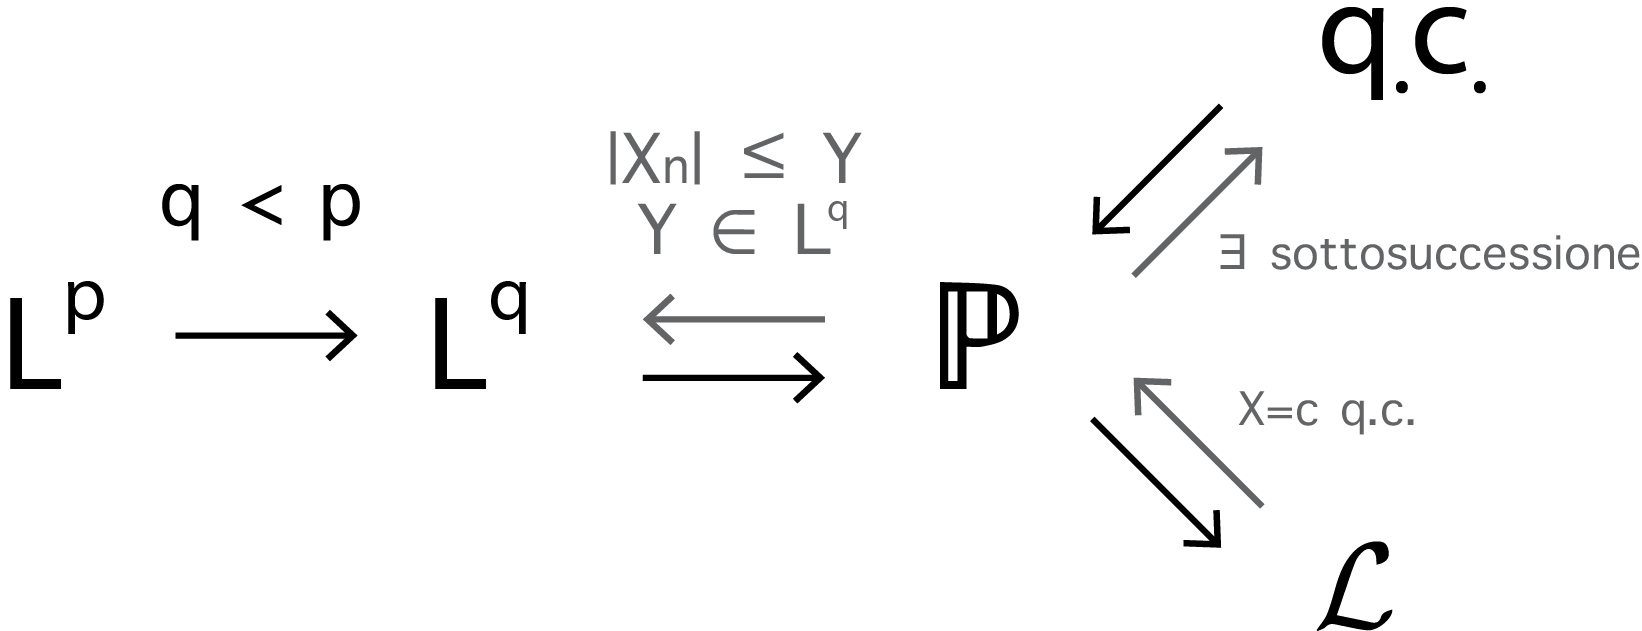
\includegraphics[width=0.5\textwidth]{img/schema_convergenza.png}
  \caption{schema riassuntivo dei teoremi sulle relazioni tra i teoremi della convergenza}
\end{figure}
\begin{itemize}
  \item La convergenza in probabilità ha una sottosuccessione che converge quasi certamente per il teorema \ref{teo-conv-prob-qc};
  \item Dati $p$ e $q$ con $p \geq q$, la convergenza in $L^p$ implica la convergenza in $L^q$ per la proposizione \ref{prop-rel-conv};
  \item Dati $|X| \in L^p$, $\ |X_n| \le Y$ qc $\ \forall n$ e $\ Y \in L^p$, ovvero rispettano una convergenza dominata e sono in $L^p$, allora è possibile, data la convergenza in probabilità, ottenere quella in $L^p$ come enunciato dal teorema \ref{teo-conv-prob-lp};
  \item Se $X_n$ converge ad una costante allora la convergenza in legge implica quella in probabilità, per il teorema \ref{conv-costante}.
\end{itemize}

\cleardoublepage

\lezione{26}{09.06.17}

\section{Teoremi limite}
I due \emph{teoremi limite} sono tra i risultati più potenti dello studio della probabilità.
Partendo da ipotesi minime, contribuiscono a mettere le basi per lo studio della statistica;
essi poggiano su tutta la teoria affrontata finora, in particolare sulla convergenza di variabili aleatorie, ma avranno delle dimostrazioni sorprendentemente semplici a questo punto della trattazione.

La \emph{legge dei grandi numeri} permette l'approssimazione della media di una variabile aleatoria attraverso esperimenti ripetuti;
il \emph{teorema centrale del limite} cementa definitivamente l'importanza della legge gaussiana nello studio di variabili aleatorie con legge \emph{qualsiasi}.
L'introduzione di questi teoremi consentirà l'analisi del \emph{comportamento asintotico} di alcune successioni (in particolare della loro \emph{velocità di convergenza}) e la \emph{stima dei parametri} di una popolazione, tecnica frequentemente sfruttata in statistica.

\subsection{Legge dei grandi numeri}\label{legge-grandi-numeri}

\begin{teo} [legge forte dei grandi numeri (LGN) \JPTh{20.1,20.2}]
  \index{legge!dei grandi numeri (LGN)}
  Siano $X_n \in L^1$ una successione di variabili aleatorie iid e $\mu \in \RR$. Allora:
  $$\EE[X_n]=\mu \iff \widebar X_n \stackrel{\text{qc}}{\longrightarrow} \mu$$
  Inoltre in questo caso vale anche $\widebar X_n \stackrel{L^1}{\longrightarrow} \mu $.
\end{teo}
Questa legge viene definita ``forte'' perché dà un risultato di convergenza quasi certa, che è ovviamente un risultato più potente rispetto ad altri tipi di convergenza. \\*
Si noti che la parte ($\implies$) di questo teorema ha ipotesi sul codominio e dà una tesi sul dominio.\footnote{``Teoremi come questi non li avete visti in analisi''} \\*
Inoltre, nel caso in cui le VA della successione siano continue, si può notare che la loro media, per definizione un integrale e quindi una somma \emph{continua}, possa anche essere ottenuta come un limite \emph{numerabile}.\\[-9pt]


Abbiamo già visto una delle applicazioni (inconsapevoli) di questo enunciato all'inizio del testo, a pagina \pageref{come-assegnare-prob}, per assegnare una probabilità in modo frequentista.

\medskip
\begin{ese}
  Se $X_n \sim Be(p)$ iid, allora $\EE[X_n]=\PP(X_n=1)=p \iff \widebar X_n \stackrel{\text{qc}}{\longrightarrow} p$.
\end{ese}

\begin{ese}
  Se $X_n \sim P^X$ iid, $\PP(X_n \in B)=P^X(B)=p \iff \dfrac{\sum_{k=1}^n \Ind_B(X_k)}{n} \stackrel{\text{qc}}{\longrightarrow} p$.
\end{ese}

\begin{ese}
  Definiamo $\Omega = \left \{ 0, \, 1 \right \}^\NN, \ \Ac=\sigma(X_n=1 \, : \, n \in \NN) $ e $ X_n(\omega)=\omega_n$. Allora si ha $\widebar X_n(\omega)=\widebar{\omega}_n \stackrel{\text{qc}}{\longrightarrow} p$.
  In questo teorema vengono definiti solo oggetti che dipendono dalla legge: in quest'ultimo caso, alterando il parametro $p$ la probabilità si sposta, senza modificarsi, andandosi a concentrare su certi $\omega_n$ che fanno tendere la media campionaria a $p$.
  Per questo il teorema funziona per ogni valore ammissibile di $p$.
\end{ese}
\medskip

\begin{prop}
  Siano $X_n$ VA iid in $L^2$. Allora:
  $$\mu= \EE[X_n] \text{ e } \sigma^2=Var(X_n) \ \implies \ S^2_n \stackrel{\text{qc}}{\longrightarrow} \sigma^2$$
\end{prop}

\begin{dimo}
  Possiamo riscrivere $S^2_n$ a partire dalla sua definizione:
  $$S^2_n = \dfrac{1}{n-1} \sum_{k=1}^{n}(X_k-\widebar X_n)^2 =
  \dfrac{n}{n-1} \left[\frac{1}{n} \cdot \sum_{k=1}^{n} X_k^2 - \widebar X_n^2\right]$$
  Analizziamo ora la convergenza di ciascun elemento:
  $$ \dfrac{n}{n-1} \stackrel{n}{\longrightarrow} 1, \qquad
  \frac{1}{n}\sum_{1}^{n}X_k^2 \; \stackrel{\text{qc}}{\longrightarrow} \; \EE[X^2] = \mu^2 + \sigma^2, \qquad
  \widebar X_n^2 \stackrel{\text{qc}}{\longrightarrow} \mu^2$$
  Per le proprietà della convergenza quasi certa, $S^2_n \stackrel{\text{qc}}{\longrightarrow} 1(\mu^2 + \sigma^2 - \mu^2)=\sigma^2$.
\end{dimo}

\medskip
\begin{dimo}[\hspace{-3pt}della LGN]
  Dimostreremo solo ($\implies$) nel caso $L^2$. \\
  Siano $X_n \in L^2$ iid e chiamiamo $\mu = \EE[X_n]$ e $\sigma^2 = Var(X_n)$ per semplicità di notazione.
  % \implies \widebar X_n \stackrel{\text{qc}}{\longrightarrow} \mu$.\\

  \begin{enumerate}
    \item Dimostriamo che $\widebar X_n \stackrel{L^2}{\longrightarrow} \mu$.
    Per linearità del valore atteso possiamo affermare che $\EE[\widebar X_n]=\mu$ e che:
      $$Var(\widebar X_n)= \EE[(\widebar X_n - \mu)^2] =\dfrac{\sigma^2}{n} \stackrel{n}{\longrightarrow} 0$$
      Da ciò discende immediatamente l'affermazione di sopra.

      Possiamo quindi imporre $\mu=0$ senza perdita di generalità definendo la VA $Y_n \coloneqq X_n-\mu$, infatti:
      $$\EE[X_n]=\mu, \ \widebar X_n \stackrel{\text{qc}}{\longrightarrow} \mu \iff \EE[Y_n]=0, \  Y_n \stackrel{\text{qc}}{\longrightarrow} 0$$

    \item Mostriamo ora che la sottosuccessione $\widebar X_{n^2}$, ovvero la media campionaria degli $X_k$ tali che $k=n^2$ per un qualche $n$, converge quasi certamente a 0.
      \begin{align*}
      	\EE \left[ \sum_{n=1}^{+\infty}(\widebar X_{n^2})^2 \right] &= \sum_{n=1}^{+\infty} \EE\left[ (\widebar X_{n^2})^2 \right] &\text{(scambio di limiti \ref{teo-leibniz-style} con VA positive)}\\
      	&= \sum_{n=1}^{+\infty} Var(\widebar X_{n^2}) &\text{(perché $\EE[X_n]=0$)} \\
      	&= \sum_{n=1}^{+\infty} \dfrac{\sigma^2}{n^2} < +\infty &\text{(la serie di $\frac 1{n^2}$ converge)}
      \end{align*}
      Condizione necessaria per la convergenza della serie è che il limite del termine generale della successione valga zero:
      $$\sum_{n=1}^{+\infty}( \widebar X_{n^2} )^2 < +\infty \ \text{qc} \ \implies ( \widebar X_{n^2})^2 \stackrel{n}{\longrightarrow} 0 \ \text{qc} \ \iff \widebar X_{n^2} \stackrel{\text{qc}}{\longrightarrow} 0$$

    \item Infine proviamo che $\widebar X_n \stackrel{\text{qc}}{\longrightarrow} 0$.\\
      Sia $p(n) \in \NN$ il numero\footnote{Formalmente si può definire questo numero come $p(n) \coloneqq \lfloor{\sqrt n}\rfloor$, che è un valore ben definito per ogni $n$. Tale definizione non è comunque rilevante ai fini della dimostrazione.} tale che:
      $$p(n)^2 \le n < (p(n)+1)^2, \ \ \text{ovvero} \ \ \frac{(\sqrt{n}-1)^2}{n} < \frac{p(n)^2}{n} \le 1$$
      Per il teorema dei due carabinieri, vale che $\frac{p(n)^2}{n} \stackrel{n}{\longrightarrow}1$. \\
      Sfruttiamo $p(n)$ per definire una nuova VA:
      $$\widebar X_n - \dfrac{p(n)^2}{n} \widebar X_{p(n)^2} = \dfrac{1}{n} \sum_{k= p(n)^2+1}^{n} X_k$$
      Passando alle varianze:
      $$ Var \left( \widebar X_n - \dfrac{p(n)^2}{n} \widebar X_{p(n)^2} \right)
      = Var \left( \dfrac{1}{n} \sum_{k= p(n)^2+1}^{n} X_k \right)
      = \dfrac{1}{n^2} \sigma^2 \left(n-p(n)^2 \right)$$
      Con una catena di minorazioni, troviamo:
      $$\dfrac{1}{n^2} \sigma^2 \left(n-p(n)^2 \right)
      \le \dfrac{\sigma^2}{n^2} (2p(n)+1)
      \le \dfrac{\sigma^2}{n^2} \left(2 \sqrt{n}+1 \right)
      \le \dfrac{3 \sigma^2}{n^{\frac{3}{2}}}$$
      Sviluppando la varianza tramite la definizione e sfruttando la linearità del valore atteso, abbiamo:
      \begin{align*}
        \EE \left[ \sum_{n=1}^{+\infty} \left( \widebar X_n - \dfrac{p(n)^2}{n} \widebar X_{p(n)^2} \right)^2 \right]
        &= \sum_{n=1}^{+\infty} \EE \left[ \left(\widebar X_n - \dfrac{p(n)^2}{n} \widebar X_{p(n)^2} \right)^2 \right]\\
        &\le \sum_{n=1}^{+\infty} \dfrac{3 \sigma^2}{n^ {\frac{3}{2}} } < +\infty
      \end{align*}
      Si ottiene così una serie convergente; quindi, come abbiamo già visto, il termine generale tende a $0$. Rimuoviamo allora il quadrato:
      $$ \left( \widebar X_n - \dfrac{p(n)^2}{n} \widebar X_{p(n)^2} \right)^2 \stackrel{\text{qc}}{\longrightarrow} 0
      \implies \widebar X_n - \dfrac{p(n)^2}{n} \widebar X_{p(n)^2}  \stackrel{\text{qc}}{\longrightarrow} 0 \ $$
      Sfruttando i risultati precedenti vediamo che:
      $$\widebar X_n =
      \underbrace{ \widebar X_n - \dfrac{p(n)^2}{n} \widebar X_{p(n)^2} }_{\stackrel{\text{qc}}{\longrightarrow} 0} +
      \underbrace{ \dfrac{p(n)^2}{n}}_{\longrightarrow 1} \cdot
      \underbrace{ \widebar X_{p(n)^2} }_{\stackrel{\text{qc}}{\longrightarrow} 0}  \stackrel{\text{qc}}{\longrightarrow} 0 \qedhere$$
  \end{enumerate}
\end{dimo}

\subsubsection{Applicazioni notevoli}
\emph{Metodo Monte Carlo.} Vogliamo stimare numericamente il seguente integrale:
$$c= \int_0^1 h(x) \, \dx, \ \  \text{con } h \in L^1$$
Per farlo definiamo $X_n \sim U([0,1])$ iid. Notiamo che $h(X_n) \in L^1(\PP)$ iid $\iff h \in L^1(P^{X_n})$. Allora:
$$\frac{1}{n} \sum_{k=1}^{n} h(X_k) \stackrel{\text{qc}}{\longrightarrow} \EE[h(X_1)]=\int_{0}^{1}h(s) \, \de s \\
\implies \frac{1}{n} \sum_{k=1}^{n}h(X_k) \simeq c \quad \text{(se $n$ è grande)}$$
In generale, il metodo Monte Carlo è una tecnica che calcola integrali approssimandone il valore con la media campionaria, anche se la funzione integranda non ammette integrale elementare.

\medskip
\emph{Statistica.} Tramite la consistenza è possibile stimare $\mu$ e $\sigma^2$:
$$\widehat{\mu}=\widebar X_n \stackrel{n}{\longrightarrow} \mu \qquad \text e \qquad \widehat{\sigma}^2= S_n^2= \dfrac{1}{n-1} \sum_{k=1}^{n}(X_k-\widebar X_n)^2$$

\subsection{Teorema centrale del limite}

\begin{teo}[teorema centrale del limite (TCL) \JPTh{21.1}]\label{TCL}
  \index{teorema!centrale del limite (TCL)}
  Siano $X_n$ iid in $L^2$, con $\mu = \EE[X_n]$ e $\sigma^2= Var(X_n)>0$. Allora:
  $$\dfrac{\widebar X_n-\mu}{ \dfrac{\sigma}{\sqrt{n} } }  \stackrel{\Lc}{\longrightarrow} \Nc(0,1)$$
\end{teo}
Se $\sigma^2=0$ il teorema perde di significato, ma questo è comunque un caso di banale trattazione.

Nella pratica statistica questo teorema risolve il problema dell'impossibilità di fare infiniti esperimenti: considerando un campione sufficientemente numeroso, la distribuzione può essere approssimata con una gaussiana.\footnote{``La statistica, di colpo, serve a qualcosa''}

\begin{nb}
  Dati $X_n \in L^2$ iid, abbiamo visto che, per la legge dei grandi numeri, $\widebar X_n \stackrel{\text{qc}}{\longrightarrow} \mu$ e che la varianza della media campionaria si riduce fino a diventare nulla:
  $$Var(\widebar X_n)=\dfrac{\sigma^2}{n} \longrightarrow 0$$
  Dunque la distribuzione si stringe e converge in legge a $\delta_{\mu}$, a prescindere dalla legge originaria delle VA.
  Normalizzando si impedisce che essa degeneri in una delta, permettendo l'osservazione della distribuzione per $n$ che tende ad infinito:
  $$ \dfrac{\widebar X_n - \mu}{\dfrac{\sigma}{\sqrt{n}}} \ \implies \
  \EE \left[ \dfrac{\widebar X_n - \mu}{\dfrac{\sigma}{\sqrt{n}}} \right] = 0, \quad
  Var \left( \dfrac{\widebar X_n - \mu}{\dfrac{\sigma}{\sqrt{n}}} \right) = 1 $$
\end{nb}
Senza il teorema, il limite del rapporto nella tesi sarebbe un'irrisolvibile forma indeterminata $\frac 0 0$.

Le ipotesi del TCL (o delle sue varianti) possono, in alcuni casi, non richiedere che le VA siano iid, e ciò spiega perché le distribuzioni gaussiane siano così comuni: essendo molte VA somme di diversi componenti indipendenti, gli effetti del TCL si ripercuotono su tali casi.
Un esempio può essere l'altezza, dovuta a molti fattori diversi che la influenzano in modo non identicamente distribuito; infatti, preso un numero sufficientemente elevato di individui, essa risulta gaussiana.

\lezione{27}{14.06.17}

\medskip
\begin{dimo}[\hspace{-3pt}del TCL]
	Questa dimostrazione fa uso del logaritmo complesso, argomento tipicamente sviscerato nel corso di analisi 3.
	Per agevolare la comprensione si possono trovare alcuni cenni alle sue proprietà nell'appendice A, a pagina \pageref{log-complesso}.

  Come per la LGN, è possibile porre $\mu = 0$ senza perdita di generalità mediante la traslazione $Y_n \coloneqq X_n - \mu$.
  Infatti questo implica che $Y_n$ iid,  $Y_n \in L^2$, $\EE [Y_n] = 0$, $\widebar{Y}_n = \widebar X_n - \mu$, $Var(Y_n) = \sigma^2$, e che pertanto:
  $$\frac{\widebar{Y}}{\frac{\sigma}{\sqrt{n}}} = \frac{\widebar X_n - \mu}{\frac{\sigma}{\sqrt{n}}} \stackrel{\Lc}{\longrightarrow} \Nc(0,1)$$

  Avendo una convergenza in legge è opportuno usare la funzione caratteristica: sia dunque $\varphi$ la funzione caratteristica di $Y_n$.
  Si nota che $\varphi(u) = \EE[e^{iuY_n}] \implies \varphi \in C^2$ perché $Y_n \in L^2$ e perché $\varphi'(0) = 0$ e $\varphi''(0) = -\sigma^2$, valori che si possono facilmente verificare. Pertanto, lo sviluppo in serie di Taylor arrestato al second'ordine di $\varphi$ è:
  $$\varphi(u) = 1 - \frac{1}{2}\sigma^2 u^2 + o(u^2), \quad \text{con } o(u^2) \in \CC$$
  Si può ora scrivere la $\varphi$ del rapporto cercato e modificarla nel modo che segue:
  \begin{align*}
    \varphi_{\frac{\widebar{Y}_n}{\sigma}\sqrt{n}}(u) \;
    &= \; \varphi_{\frac{\sum\limits_{k=1}^{n} Y_k}{\sigma \sqrt{n}}} (u) \;
    	= \; \varphi_{\sum\limits_{k=1}^{n} Y_k}\left( \frac{u}{\sigma \sqrt{n}} \right)
   	&\mathmakebox[1pt][r]{\hfill\text{(per le proprietà di $\varphi$)}}\\
    &= \; \left( \varphi \left( \frac{u}{\sigma \sqrt{n}} \right) \right)^n
    	&\mathmakebox[1pt][r]{\hfill\text{(le VA sono iid)}}\\
    &= \exp\left\{\log\left( \varphi \left( \frac{u}{\sigma \sqrt{n}} \right) \right)^n\right\}
	&\mathmakebox[1pt][r]{\hfill\text{(introducendo un exp)}}\\
    &= \exp\left\{n \log\left( \varphi \left( \frac{u}{\sigma \sqrt{n}} \right) \right)\right\} 
	&\mathmakebox[1pt][r]{\hfill\text{(proprietà dei logaritmi)}}\\
    &= \exp \left\{ n \log\left( 1-\frac{1}{2} \sigma^2 \frac{u^2}{n\sigma^2} + o \left( \frac{1}{n} \right) \right) \right\}
    	&\mathmakebox[1pt][r]{\hfill\text{(sviluppando in serie $\varphi$)}}\\
    &= \exp \left\{ n \left( -\frac{1}{2} \frac{\sigma^2 u^2}{n \sigma^2} + o \left( \frac{1}{n} \right) \right) \right\}
    	&\mathmakebox[1pt][r]{\hfill\text{(sviluppando in serie il log)}}\\
    &= \exp \left\{ \left( -\frac{1}{2} u^2 + o (1) \right) \right\}
    \stackrel{n \to +\infty}{\longrightarrow} e^{-\frac{u^2}{2}} = \varphi_{\Nc(0,1)}(u) \ \forall u \in \RR
	\qquad \quad %eh lo so che sono una brutta persona (AW)
  \end{align*}
  Questo conclude la dimostrazione.
  Si noti ancora come essa regga per qualsiasi distribuzione, dipendendo solo da media e varianza della legge.
\end{dimo}

\subsection{Comportamento asintotico di alcune distribuzioni}
L'introduzione del TCL permette uno studio dell'andamento delle distribuzioni di una successione di VA $X_1,\dots,X_n$ quando $n$ è sufficientemente grande.
Forniamo di seguito qualche esempio notevole.

\subsubsection{Chi-quadro}
Data una successione di VA $X_n \sim \chi^2(n)$, si ha $X_n \sim \sum\limits_{k=1}^{n} Z_k^2$, dove $Z_k \sim \Nc(0,1)$ iid. Notiamo che anche $Z_k^2 \sim \chi^2(n)$ iid.

I momenti della $Z_k^2$ sono $\EE[Z_k^2] = 1$ e $Var(Z_k^2) = 2 \enspace \forall k$, quindi possiamo procedere con la normalizzazione, come richiesto dal TCL:
$$\frac{X_n - n}{\sqrt{2n}} \sim \frac{\sum\limits_{k=1}^{n} Z_k^2 - n}{\sqrt{2n}} = \frac{\widebar{(Z_n^2)} - 1}{\sqrt{\frac{2}{n}}}
\; \stackrel{\Lc}{\longrightarrow} \; \Nc(0,1) $$ %è la media campionaria degli Z_n^2, quindi il \widebar va sopra tutto quanto (Br1)
Per $n$ grande, si ha:
$$\frac{X_n-n}{\sqrt{2n}} \approx \Nc(0,1) \implies X_n \sim \chi^2(n) \approx \Nc(n,2n)$$
\begin{nb}
	Si nota che, come sempre parlando di leggi, non è detto che $X_n$ sia effettivamente una somma di normali standard, ma semplicemente ha la stessa distribuzione di una somma di normali standard.
\end{nb}

\subsubsection{$t$ di Student}
Data una successione di VA $X_n \sim t(n)$, si ha $X_n \sim \frac{Z}{\sqrt{Q/n}} \;$, dove $Z \sim \Nc(0,1),$ \\*
$Q \sim \chi^2$ e $Z \indep Q$.

Grazie alla LGN possiamo mostrare che:
$$\frac{Q}{n} \sim \frac{\sum\limits_{k=1}^{n} Z_k^2}{n} \stackrel{\text{qc}}{\longrightarrow} 1
\implies \frac{Q}{n} \stackrel{\Lc}{\longrightarrow} 1
\implies X_n \sim \frac{Z}{\sqrt{\frac{Q}{n}}} \stackrel{\Lc}{\longrightarrow} \Nc(0,1)$$
Per l'ultima implicazione abbiamo invocato Slutsky\footnote{Che è il nuovo Fubini-Tonelli.}, affermando che $Q/n$ tende ad una costante.
In altri termini, si è ottenuta la seguente relazione tra leggi:
$$t(n) \xrightarrow{\text{deb}} N(0,1)$$

\subsubsection{Binomiale}
Data una successione di $X_n \sim Bi(n,p)$, si ha $X_n \sim \sum\limits_{k=1}^{n} Y_k$, dove $Y_k \sim Be(p)$ iid.\\
Ne consegue che $X_n \sim n\widebar{Y}_n$.
Per il TCL si scrive che: $$\frac{\widebar{Y}_n - p}{\sqrt{np(1-p)}/n} \stackrel{\Lc}{\longrightarrow} \Nc(0,1) \implies \frac{X_n - np}{\sqrt{np(1-p)}} \stackrel{\Lc}{\longrightarrow} \Nc(0,1)$$\\
Ovvero, dato $n$ grande, la generica relazione tra le due leggi è la seguente:
$$Bi(n,p) \approx \Nc(np, np(1-p))$$

\subsection{Velocità di convergenza}

Data una successione di VAR $X_k$ iid in $L^2$, indicata con $\widebar X_n$ la loro media campionaria per $n \to +\infty$ si ha:
\begin{itemize}
	\item $\widebar X_n \stackrel{\text{qc}}{\longrightarrow} \mu$ per la legge dei grandi numeri;
	\item $\sqrt{n}(\widebar X_n - \mu) \stackrel{\text{qc}}{\longrightarrow} \Nc(0, \sigma^2)$ per il teorema centrale del limite.
\end{itemize}
L'ultimo criterio viene utilizzato per misurare la \textit{velocità di convergenza} del limite.

Riprendiamo una definizione dall'analisi per agevolare la spiegazione:

\begin{defn}\label{vel-conv-falza}
  La \emph{velocità di convergenza} della funzione $f(x)$ è l'esponente $\alpha$ tale per cui: $$\lim\limits_{x \to +\infty} x^\alpha f(x) = L \in \RR \setminus \{0\}$$
\end{defn}

\medskip
\begin{ese}
  Data la funzione $\cos\left(\frac 1 n\right) \stackrel{n}{\to} 1$, l'espressione $n^\alpha \left(\cos\left(\frac 1 n\right)-1\right)$ tende ad un limite finito diverso da zero per $\alpha = 2$.
\end{ese}

\medskip
\begin{defn}
  \index{convergenza!velocità di}
  Sia $X_n$ una successione di VAR, $a \in \RR$ una costante, e $v_n$ una successione reale con $v_n \; \to +\infty$ per $n \to +\infty$. \\*
  Se $\exists \, T$ VAR, con $ T \nsim \delta_0 $, tale che $v_n(X_n-a) \stackrel{\Lc}{\longrightarrow} T$, allora si dice che $X_n$ converge ad $a$ con \textbf{velocità di convergenza $v_n$}.
\end{defn}

\medskip
\begin{nb} La distribuzione $\delta_0$ prevede tutta la probabilità concentrata nel punto 0:
  $T \nsim \delta_0 \iff \PP (T=0) < 1$. La distribuzione limite $\delta_0$ è dunque l'analogo del limite nullo nel caso presentato nella definizione \ref{vel-conv-falza}.
\end{nb}

\medskip
\begin{nb}$X_n \stackrel{\Lc}{\longrightarrow} a \implies X_n \stackrel{\PP}{\longrightarrow} a$. Infatti
  $X_n - a = \underbrace{v_n(X_n-a)}_{\to T}\underbrace{1/v_n}_{\to 0} \xrightarrow{n} 0$ per il teorema di Slutsky.
\end{nb}

\begin{ese}
  Sia $X_k$ una successione di VA iid in $L^2$ con $\sigma_k^2 > 0 \enspace \forall k$; allora la media campionaria $\widebar X_n$ converge a $\mu$ con velocità $v_n = \sqrt n$, \emph{a prescindere dalla legge delle $X_k$}.
  Infatti, applicando il TCL, si ha che $\sqrt{n}(\widebar X_n - \mu) \longrightarrow \Nc(0, \sigma^2)$. \\*
  Questo risultato, data la sua generalità, viene spesso utilizzato negli esercizi per indovinare la velocità di convergenza di successioni più complesse.
\end{ese}

\medskip
\begin{nb}
  $v_n$ non è univocamente determinata. Infatti, data una successione $X_n \to \mu$ con $v_n = \sqrt{n}$, questa converge a un valore reale non nullo anche, per esempio, per $v_n' = \frac{n}{n+1}\sqrt{n} \,$ grazie al teorema di Slutsky.
\end{nb}

\begin{ese}
  Si consideri una successione di VA $X_k \sim U([0, \lambda])$ iid con $\lambda > 0$ fissato. Sia poi $X_{(1)} = \min\{X_1, \dots, X_n\} = W_n$.\footnote{Il pedice $(1)$ è una notazione alternativa per il minimo frequentemente usata in statistica. Più in generale, dato un insieme di valori $\{X_1,\dots,X_n\}$, $X_{(i)}$ è l'$i$-esimo valore più piccolo dell'insieme (e quindi $X_{(n)}$ è il valore massimo tra essi).}
  Dimostriamo che $W_n$ tende in legge a 0. \\*
  Si utilizza, come spesso succede quando sono coinvolti dei min, la funzione di ripartizione di $W_n$: essa è $F_{W_n} (t) = \PP(W_n \leq t) = 1-\PP(W_n > t)$. Tuttavia, essendo $W_n$ un minimo di VA iid, $F_{W_n}(t) = 1-\PP(X_1 > t, \dots, X_n > t) = 1- \PP (X_1 > t)^n$. Distinguiamo quindi i casi per la variabile $t$:

  $$F_{W_n} (t) = \begin{cases} 0 &\text{per }t \leq 0 \\ 1-\left( \frac{\lambda-t}{\lambda}\right)^n &\text{per }0 < t \leq \lambda \\ 1 &\text{per }t > \lambda \end{cases} \quad \stackrel{n \to +\infty}{\longrightarrow} \quad \begin{cases} 0 &\text{per }t \leq 0 \\ 1 &\text{per }0 < t \leq \lambda \\ 1 &\text{per }t > \lambda \end{cases} \; = \;\Ind_{(0, +\infty)} (t)$$

  Si può quindi affermare che $F_{W_n}(t) \stackrel{\text{qo}}{\longrightarrow} \Ind_{[0, +\infty)} (t) \enspace \forall t$ (per la precisione, ovunque tranne che in $t=0$).
  Ma questa è la funzione di ripartizione della delta di Dirac $\delta_0$, quindi $W_n \stackrel{\Lc}{\longrightarrow} 0$.

  In questo caso la velocità di convergenza è $v_n = n$: infatti, si può dimostrare che $n W_n = T_n \stackrel{\Lc}{\longrightarrow} \varepsilon(\lambda)$.
\end{ese}

\subsubsection{Asintotica normalità}

\begin{defn}
  \index{asintotica normalità}
  Una successione di VA è detta \textbf{asintoticamente normale} di parametri $a$ e $\frac{q}{v_n^2}$ (con $q > 0$ e $v_n \to +\infty$) se:
  $$v_n(X_n-a) \stackrel{\Lc}{\longrightarrow} \Nc(0, q), \quad \text{e si scriverà }
  X_n \sim  AN \left(a,\frac{q}{v_n^2}\right)$$
\end{defn}

\medskip
\begin{ese}
  Riscriviamo il TCL con la notazione appena introdotta:
  $$
    X_k \text{ iid in } L^2, \text{ con } \sigma^2 > 0 \ \implies \ \widebar X_n \sim AN \left( \mu, \frac{\sigma^2}{n} \right)
  $$
\end{ese}

\medskip
\begin{nb}
  Nonostante $X_n \to a$, non è necessariamente vero che $\EE[X_n] \longrightarrow a$ o che $Var(X_n) \sim \frac{q}{v_n^2}$.
\end{nb}

\medskip
\begin{cese}
	Siano $X_n, Y_n$ successioni di VAR tali che $X_k \indep Y_k \ \forall k$. Siano inoltre $p_n, \mu_n, v_n$ e $\sigma_n$ successioni numeriche tali che $v_n \to +\infty$, che $Y_n \sim Be(p_n)$ con $p_n \xrightarrow{n} 1$, e che le $X_n$ abbiano, per ogni $n$, la seguente legge condizionata:
	$$X_n | Y_n = k \sim \Nc \left( ak + \mu_n(1-k), k \frac q {v_n^2} + (1-k) \frac{\sigma_n^2}{v_n^2} \right)$$
	Dimostriamo che $X_n$ è asintoticamente normale, ovvero che $Z_n = v_n(X_n - a) \xrightarrow{\Lc} \Nc(0,q)$. Mediante il teorema \ref{phi-trasf-aff} sulle trasformazioni affini delle funzioni caratteristiche si ottiene:
	$$ \varphi_{Z_n}(u) = e^{-i a v_n u} \varphi_{X_n}(v_n u)$$
	Ricordando che $\varphi_{X_n}$ è un valore atteso e che pertanto vale la formula di pagina \pageref{formula-att-cond}, si può continuare scrivendo:
	\begin{align*}
		e^{-i a v_n u} &\varphi_{X_n}(v_n u) = e^{-i a v_n u} \Ex { \ \varphi_{X_n}(v_n u) \ } \\[7pt]
		&= e^{-i a v_n u} \Big[ p \ \Ex { \ \varphi_{X_n}(v_n u) \ | Y_n=1 } + (1-p) \ \Ex { \ \varphi_{X_n}(v_n u) \ | Y_n=0 } \Big] \\
		&= e^{-i a v_n u} \left[ p \ \varphi_{\Nc \left( a, \frac q {v_n^2} \right) }(v_n u) + (1-p) \ \varphi_{\Nc \left( \mu, \frac {\sigma_n^2} {v_n^2} \right)} (v_n u) \right]
	\end{align*}
	Infatti $k=0$ o $k=1$ cancellano l'uno o l'altro dei due addendi nei parametri della legge di $X_n | Y_n = k$. Ora, la funzione caratteristica $\varphi_{\Nc \left( \mu, \frac {\sigma_n^2} {v_n^2} \right)} (v_n u)$ è limitata $\forall u$ e $1-p \to 0$: l'intero secondo addendo è un $o(1)$. Sostituendo la formula per la $\varphi_{\Nc}$ nell'addendo rimasto e ricordando che $v_n \to +\infty$, risulta che:
	\begin{align*}
		\varphi_{Z_n}(u) &= e^{-i a v_n u} \Big[ p \ e^{i a v_n u - \frac 1 2 \frac q {v_n^2} v_n^2 u^2} + o(1) \Big] \\[7pt]
		&= p \ e^{- \frac 1 2 q u^2} + e^{-i a v_n u} o(1) \overset{n}{\longrightarrow} e^{- \frac 1 2 q u^2 }
	\end{align*}
	La funzione ottenuta è la funzione caratteristica di una normale con media nulla e varianza $q$. Dunque effettivamente $ X_n \sim \Ac\Nc\left( a, \frac q {v_n^2} \right)$. Infine, calcoliamo media e varianza di $X_n$ usando le definizioni di attesa e varianza condizionata:
	\begin{align*}
		\Ex{X_n} &= \EE \big[ \Ex{X_n | Y_n} \big] \\
		&=\Ex{ a Y_n + \mu_n (1-Y_n) } = a \ p_n + (1 - p_n) \mu_n\\[10pt]
		Var(X_n) &=\ Var ( \Ex{X_n|Y_n} ) + \Ex{ Var( X_n|Y_n ) } & (\text{proprietà \ref{scomp-var}})
	\end{align*}
	Quindi per le proprietà di varianza e valore atteso si ha:
	\begin{align*}
		Var(X_n) &= Var \big(aY_n + \mu_n(1-Y_n)\big) + \Ex{ Y_n \frac q {v_n^2} + (1-Y_n) \frac{\sigma_n^2}{v_n^2} } \\
		&= (a - \mu_n)^2 p (1-p) + p \frac q {v_n^2} + (1-p) \frac{\sigma_n^2}{v_n^2}
	\end{align*}
	Come si può osservare, media e varianza non sono sempre uguali, rispettivamente, ad $a$ e a $\frac q {v_n^2}$; anzi, a seconda delle successioni scelte nelle ipotesi si può farle convergere a qualsiasi valore desiderato o anche divergere a $+\infty$.
\end{cese}

Data una funzione $h:\RR \to \RR$ continua e $X_n$ che converge in legge, probabilità o quasi certa\footnote{``Nel modo che preferite'', disse Gregoratti.} $X_n \longrightarrow a$ allora è noto che $Y_n = h(X_n) \implies Y_n \longrightarrow h(a)$, ma per scoprire la sua velocità di convergenza e se è asintoticamente normale introduciamo il metodo delta 1, molto utile negli esercizi.
\medskip

\begin{teo}[metodo delta 1\footnote{Nel caso ve lo steste chiedendo: sì, esiste un metodo delta 2, ma non fa parte del programma di questo corso.}]
  \index{metodo delta 1}
  Siano:
  \begin{itemize}
    \item $X_n$ successione di VA reali a valori in un boreliano $B \subseteq \RR$;
    \item $a \in \mathring{B}$, ovvero punto interno a $B$;
    \item $v_n \to +\infty$, velocità di convergenza;
    \item $T$ VAR.
  \end{itemize}
  Se $v_n(X_n - a) \stackrel{\Lc}{\longrightarrow} T$ e $h:B \to \RR$ è una funzione misurabile su $B$ e differenziabile in $a$, allora:
  $$v_n(h(X_n) - h(a)) \; \stackrel{\Lc}{\longrightarrow} \; h'(a) T $$
\end{teo}
Si noti che la funzione $h$ non deve dipendere da $n$, altrimenti $h$ non sarebbe una funzione, bensì una successione di funzioni $h_n$ e il metodo delta 1 non sarebbe valido.
\needspace{3\baselineskip}
\begin{dimo}
	\Fixvmode
	\begin{itemize}
		\item \emph{Caso generale.}
		Si scriva lo sviluppo di Taylor-Peano di $h(x)$ centrato in $x = a$:
		$$h(x) = h(a) + h'(a) (x-a) + o(x-a) \quad \forall x \in B$$
		Si definisca ora il resto $r$ come $r(x-a) \coloneqq h(x) - h(a) - h'(a) (x-a) = o(x-a)$, con $x \in B$, che è tale che $\frac{r(x-a)}{x-a} \to 0$ per $x \to a$. Definiamo quindi anche la funzione $g: \RR\to\RR$:
		$$g(y) \coloneqq
		\begin{cases}
		\frac{r(y)} y & \text{con } y+a \in B, \; y \neq 0\\
		0       & \text{con } y+a \notin B, \; y \neq 0
		\end{cases}
		$$
		Essa è continua in $y = 0$ e misurabile. Dunque $h(x) - h(a) = h'(a) (x-a) + (x-a) g(x-a) \enspace \forall x \in B$. Applichiamo la velocità di convergenza:
		\begin{align*}
			v_n(h(X_n)-h(a)) &= v_n\big( h'(a) (X_n-a)  + (X_n-a) g(X_n-a) \big) \\
			&=v_n (X_n-a) h'(a) + v_n(X_n-a)g(X_n-a)
		\end{align*}
		I termini $v_n(X_n-a)$ convergono in legge a $T$; inoltre, poiché $X_n-a \xrightarrow{\Lc} 0$, per la continuità di $g$ anche $g(X_n-a) \xrightarrow{\Lc} g(0) = 0$. Per il teorema di Slutsky la somma converge dunque in legge a $T \cdot h'(a) + T \cdot 0 = h'(a) T$.
		\item \emph{Caso $B=\RR$}.
		$$g(s) \coloneqq
		\begin{cases}
		\frac{h(s)-h(a)}{s-a}-h'(a) & \text{per } s\neq a\\
		0       & \text{per } s = a
		\end{cases}
		$$
		Mediante uno sviluppo di Taylor al prim'ordine si può scrivere che:
		$$v_n (h(X_n) - h(a)) = v_n ( h'(a) (X_n-a) + o(X_n-a) )$$
		%Ma cos'è $v_n\cdot o(X_n-a)$? \\ %E' quello che ci stiamo chiedendo tutti (Br1)
		Portando $v_n h'(a) (X_n-a)$ al membro sinistro:
		\begin{align*}
			v_n \, o(X_n-a)
			&= v_n \big( h(X_n)-h(a)-h'(a)(X_n-a) \big) \\
			&= v_n(X_n-a) \left( \frac{h(X_n)-h(a)}{X_n-a}-h'(a) \right) \\
			&= \underbrace{v_n(X_n-a)}_{\stackrel{\Lc}{\to}T}\underbrace{g(X_n)}_{\stackrel{\Lc}{\to}g(a)}
			\xrightarrow{\Lc} 0 T = 0 &\text{(per Slutsky)}
		\end{align*}
		Pertanto, ricordando la definizione di $g$:
		\begin{align*}		
		v_n (X_n - a) &\left(\frac{h(X_n)-h(a)}{X_n-a} - h'(a) \right) \xrightarrow{\Lc} 0 \\
		&\implies v_n (h(X_n)-h(a)) - h'(a) v_n (X_n-a) \xrightarrow{\Lc} 0 \\
		&\implies v_n (h(X_n)-h(a)) \xrightarrow{\Lc} h'(a) T &\qedhere
		\end{align*}
	\end{itemize}
\end{dimo}

\medskip
\begin{coro}
  Se $T \nsim \delta_0$ e $h'(a) \neq 0$, $v_n$ è la velocità di convergenza sia di $X_n$ che di $h(X_n)$; \\*
  in altri termini, \emph{quasi} tutte le trasformazioni \emph{non} modificano la velocità di convergenza.
\end{coro}

\medskip
\begin{coro}[metodo delta 1, caso gaussiano]\label{md1-gauss}
  Siano $X_n: \Omega \to B$ tali che $X_n \sim AN \left( a, \frac q {v_n^2} \right)$ e $h: B \to \RR$ funzione misurabile tale che $h'(a) \neq 0$. Allora:
  $$Y_n = h(X_n) \sim AN \left( h(a), (h'(a))^2 \frac q {v_n^2} \right)$$
\end{coro}

\needspace{3\baselineskip}

\lezione{28}{15.06.17}

Vediamo qualche esempio di applicazione del corollario enunciato poc'anzi.

\begin{ese}
  Siano $X_n \sim \Ec (\lambda)$ iid con $\lambda > 0$. \\
  È noto che $\widebar X_n \sim AN(\frac 1 \lambda, \frac 1 {n \lambda^2})$ per il TCL, e che $\widebar X_n \xrightarrow{\text{qc}} \frac 1 \lambda$ per la LGN.
  Da qui si nota, peraltro, come l'asintotica normalità non sia in senso stretto una convergenza di $\widebar X_n$, bensì di una \emph{funzione} di $\widebar X_n$, per la precisione di $(\sqrt n \widebar X_n - a)$: in caso contrario sarebbe violata l'unicità del limite.

  Si supponga ora che il valore di $\lambda$ sia incognito, e che lo si voglia stimare con la successione $Y_n \coloneqq \frac 1 {\widebar X_n}$. Dunque $Y_n = h(\widebar X_n)$, con $h: B = (0, +\infty) \to \RR, \ h(t) = \frac 1 t$, che è tale che $h'(t) = - \frac 1 {t^2} \neq 0 \ \forall t \in (0,+\infty)$.
  Si osservi che in questo caso la restrizione del dominio di $h$ a un boreliano è stata fondamentale per garantire regolarità $C^1$ in ogni punto della funzione, che altrimenti non sarebbe stata derivabile in $t = 0$.

  Per le proprietà di convergenza quasi certa e funzioni continue, $Y_n \stackrel{\text{qc}}{\longrightarrow} \lambda = a$ e quindi c'è anche convergenza in legge a $\lambda$. È dunque possibile riscrivere il limite con la notazione dell'asintotica normalità:
  $$Y_n \sim AN\left( \lambda, \big( h'(a) \big) \frac 1 {n \lambda^2} \right) = AN\left( \lambda, \frac {\lambda^4} {n\lambda^2} \right) = AN\left( \lambda, \frac {\lambda^2} n \right)$$
  Inoltre, ricordando la formula per i momenti della gamma, la quale è appunto la distribuzione di una somma di VA esponenziali, si ottiene che:
  $$\Ex{Y_n} = n \Ex{\frac 1 { \sum_{k=1}^n {X_k} } } = n \frac 1 {\lambda^{-1}} \frac{\Gamma(n-1)}{\Gamma(n)} = n \lambda \frac{(n-2)!}{(n-1)!} = \frac n {n-1} \lambda \stackrel{n}{\longrightarrow} \lambda
  $$
  Si noti che il valore atteso di $Y_n$ tende asintoticamente a $\lambda$, ma non è \emph{esattamente} $\lambda$ per ogni $n$ fissato.
  Per questa ragione lo stimatore $Y_n$ viene chiamato \emph{distorto}, definizione che preciseremo meglio nelle prossime righe.

  \index{stimatore corretto o non distorto}
  Introduciamo, infine, un'ultima successione per perfezionare ulteriormente la stima di $\lambda$: $T_n \coloneqq \frac{n-1} n \cdot Y_n = \frac{n-1}{\sum_{k=1}^n {X_k}}$, che ha valore atteso $\Ex{T_n} \equiv \lambda \ \forall n$ e viene per questo definito \emph{stimatore corretto} o \emph{non distorto}.
  Tutti gli stimatori che non sono corretti sono detti, appunto, \emph{distorti}.
  Si può inoltre mostrare che $Var(T_n) = \frac{\lambda^2}{n-2}$.

  Non rimane che studiare la convergenza: poiché $\frac{n-1}n \stackrel{n}{\longrightarrow} 1$ e $Y_n \stackrel{\text{qc}}{\longrightarrow} \lambda$, si ottiene che $T_n = \frac{n-1} n Y_n \stackrel{\text{qc}}{\longrightarrow} \lambda$, ovvero $T_n$ è asintoticamente normale. L'intuizione suggerisce che il fattore $\frac{n-1}n$ lasci inalterata la media asintotica $\lambda$ e la velocità di convergenza $\sqrt n$ di $Y_n$. In altre parole, l'aspettativa è che $\sqrt n (T_n - \lambda) \stackrel{\Lc}{\longrightarrow} \Nc(0,\lambda^2)$. Verifichiamo la correttezza della nostra \textit{Ansatz}\footnote{Come ci ricorda il buon professor Micheletti, un'\textit{Ansatz} è un'ipotesi realistica, in tedesco.}:
  $$\sqrt n (T_n - \lambda) = \sqrt n \left(\frac{n-1} n \cdot Y_n - \lambda\right) = \frac{n-1} n \sqrt n (Y_n - \lambda) + \frac{n-1} n  \sqrt n \lambda - \sqrt n \lambda$$
  Poiché $\frac{n-1}n \to 1$ (quindi anche in legge) e $\sqrt n (Y_n - \lambda) \xrightarrow{\Lc} \Nc(0, \lambda^2)$ per ipotesi, applicando il teorema di Slutsky il primo addendo converge in legge a $\Nc(0,\lambda^2)$; il secondo e il terzo addendo sommati danno $\sqrt n \lambda \frac{n-1} n \xrightarrow{n} 0$; il tutto converge dunque in legge a $\Nc(0,\lambda^2)$ e dunque effettivamente:
  $$ T_n \sim AN \left( \lambda, \frac{\lambda^2} n \right)$$
\end{ese}


\subsection{Stima dei parametri di una distribuzione} \label{applicazioni-statistica}
Un obiettivo frequente in statistica è ottenere più informazioni possibili su una popolazione $X_n$, ovvero una successione di VA iid in $L^2$, avente legge, parametri e funzione di ripartizione $F$ ignoti.
Applicando la teoria della probabilità introdurremo degli \emph{stimatori puntuali} per ciascuna delle grandezze interessate e per ciascuno stimatore elencheremo le proprietà che lo rendono efficace.
\subsubsection{Media}
Lo stimatore di $\mu = \Ex{X_n}$ è la già nota \textbf{media campionaria}: $$\widebar X_n = \frac 1 n \sum_{k=1}^n X_k$$
Infatti, a prescindere da $F$ è vero che:
\begin{enumerate}
  \index{errore quadratico medio (MSE)}
  \item $\Ex{\widebar X_n} = \mu \quad \forall n$ (stimatore corretto).
  \item $Var(\widebar X_n) = \frac{\sigma^2}n \stackrel{n}{\longrightarrow} 0$ (ovvero $\widebar X_n \stackrel{L^2}{\longrightarrow} \mu$). In termini statistici si dice che il MSE\footnote{Mean Square Error, errore quadratico medio.}$\stackrel{n}{\longrightarrow} 0$.
  \item $\widebar X_n \stackrel{\text{qc}}{\longrightarrow} \mu$ per la LGN (\textbf{consistenza}).
  \item $\dfrac{\widebar X_n-\mu}{\sfrac\sigma {\sqrt n}} \xrightarrow{\Lc} \Nc(0,1)$ per il TCL, ovvero $\widebar X_n \sim AN\left( \lambda, \frac{\sigma^2}n \right)$. \\
	Da quest'ultima proprietà discende la teoria della statistica su intervalli di confidenza e test d'ipotesi.
\end{enumerate}
Si possono visualizzare e riassumere questi risultati nel seguente grafico: \\

\begin{figure}[H]\label{plot-conv-media}
  \centering
  \begin{tikzpicture}
    \begin{axis}[
        axis lines = middle,
        xlabel = $n$,
        ylabel = $\widebar X_n$,
        width=\textwidth,
        height=0.4\textwidth,
        yticklabels={,,},
        xticklabels={,,2,4,6,8,10,12,14,\dots,n}
    ]
    \draw [line width=0.2mm, dashed] (axis cs:0,2) -- (axis cs:22,2);
    \draw [line width=0.2mm, dashed] (axis cs:18,0) -- (axis cs:18,4);

    \draw [line width=0.3mm, color=red]
      (axis cs:1,3.6) -- (axis cs:2,2.9) -- (axis cs:3,0.8) -- (axis cs:4,3) -- (axis cs:5,2.8) --
      (axis cs:6,1.0) -- (axis cs:7,1.4) -- (axis cs:8,1.7) -- (axis cs:9,1.2) -- (axis cs:10,2.5) --
      (axis cs:11,1.7) -- (axis cs:12,1.8) -- (axis cs:13,2.1) -- (axis cs:14,2.05) -- (axis cs:15,1.95) --
      (axis cs:16,2.01) -- (axis cs:17,1.99) -- (axis cs:18,2.01) -- (axis cs:19,2) -- (axis cs:20,2);

    \draw [line width=0.3mm, color=lightblue]
      (axis cs:1,1) -- (axis cs:2,3) -- (axis cs:3,3.2) -- (axis cs:4,1.5) -- (axis cs:5,0.9) --
      (axis cs:6,2.6) -- (axis cs:7,1.3) -- (axis cs:8,2.4) -- (axis cs:9,2.5) -- (axis cs:10,1.5) --
      (axis cs:11,2.2) -- (axis cs:12,2.1) -- (axis cs:13,1.95) -- (axis cs:14,1.97) -- (axis cs:15,2.03) --
      (axis cs:16,2.01) -- (axis cs:17,1.99) -- (axis cs:18,2.01) -- (axis cs:19,2) -- (axis cs:20,2);

    \addplot [draw=none, forget plot] coordinates {(-0.5,-0.5)};
    \addplot [draw=none, forget plot] coordinates {(20, 4)};

    \addplot [draw=none, forget plot] coordinates {(0,2)} node[left] {$\mu$};

    \end{axis}
  \end{tikzpicture}
  \caption{grafico della convergenza della media campionaria al valore atteso}
\end{figure}

Ogni spezzata rappresenta un diverso osservatore (supponiamo che siano in numero molto elevato) che effettua le proprie estrazioni separatamente dagli altri, aggiornando costantemente, all'aumentare del numero $n$ di campioni raccolti, la propria media campionaria. \\
Le 4 osservazioni precedenti hanno ciascuna la propria rappresentazione visuale:
\begin{enumerate}
  \item Correttezza: per ogni $n$ fissato, la media di tutti valori di $\widebar X_n$ corrispondenti a quell'$n$ (detta anche, non a caso, \emph{media verticale}) è esattamente $\mu$.
  \item Convergenza in $L^2$: lo sparpagliamento dei valori di $\widebar X_n$ intorno a $\mu$ per uno stesso $n$ diminuisce verso lo zero all'aumentare di $n$.
  \item Convergenza quasi certa: ciascuna linea spezzata rappresentante la successione $\widebar X_n$ di un osservatore tende al valore $\mu$ all'aumentare di $n$; questa quantità è anche detta media orizzontale.
  \item Convergenza in legge: un eventuale grafico della frequenza di valori di $\frac{\widebar X_n-\mu}{\sfrac\sigma {\sqrt n}}$ per uno stesso $n$ fissato tenderebbe, all'aumentare di $n$, ad avere una forma gaussiana.
\end{enumerate}

\subsubsection{Varianza}
Lo stimatore di $\sigma^2 = Var(X_n)$ è la già nota \textbf{varianza campionaria}: $$S_n^2 = \frac 1 {n-1} \sum_{k=1}^n (X_k - \widebar X_n)^2$$
Per ogni $F$:
\begin{enumerate}
  \item $\Ex{S_n^2} = \sigma^2 \quad \forall n$ (corretto).
  \item ``Non si dice cosa succede alla varianza della varianza campionaria''\footnote{Leggasi come ``Non lo vuoi davvero sapere, fidati''}
  \item $S_n^2 \stackrel{\text{qc}}{\longrightarrow}  \sigma^2$ (consistente).
  \item $\dfrac{S_n^2-\sigma^2}{\sqrt{\frac{\mu_4-\sigma^4} n}} \stackrel{\Lc}{\longrightarrow} \Nc(0,1)$, \\ ovvero $S_n^2 \sim AN\left(\sigma^2,\frac{\mu_4 - \sigma^4} n\right)$, dove $\mu_4 = \Ex{(X_n-\mu)^4} \neq \sigma^4$.
\end{enumerate}
\subsubsection{Stima di una proporzione}
\index{proporzione campionaria}
Lo stimatore della proporzione $p = \PP(X_n \in B)$ è la \textbf{proporzione campionaria}:
$$\widehat p_n = \frac 1 n \sum_{k=1}^n \Ind_B(X_k)$$
Essa non è altro che il numero dei campioni caduti effettivamente in $B$ divisi per il numero totale dei campioni. Si noti inoltre che:
$$ \Ind_B(X_k) = Y_k \sim Be(p), \quad \text{con } p = \PP(X_k \in B) = \PP(Y_k = 1)$$
Per ogni $F$, è vero che:
\begin{enumerate}
  \item $\Ex{\widehat p_n} = p \quad \forall n$ (corretto).
  \item $Var(\widehat p_n) = n \frac{p(1-p)}{n^2} = \frac{p(1-p)} n \stackrel{n}{\longrightarrow} 0$.
  \item $\widehat p_n \stackrel{\text{qc}}{\longrightarrow} p$ per la LGN.
  \item $\dfrac{\widehat p_n - p}{\sqrt{ \frac{p(1-p)} n }} \stackrel{\Lc}{\longrightarrow} \Nc(0,1)$ per il TCL. Da questa proprietà discende la teoria della statistica per i test d'ipotesi.
  \item  $\dfrac{\widehat p_n - p}{\sqrt{ \frac{\widehat p_n(1-\widehat p_n)} n }} = \dfrac{\widehat p_n - p}{\sqrt{ \frac{p(1-p)} n }} \cdot \dfrac{\sqrt{ \frac{p(1-p)} n }}{\sqrt{ \frac{\widehat p_n(1-\widehat p_n)} n }} \stackrel{\Lc}{\longrightarrow} \Nc(0,1)$ per il teorema di Slutsky. \\*
  Infatti la prima frazione converge in legge a $\Nc(0,1)$ per il punto precedente e la seconda frazione, funzione continua di $\widehat p_n$, converge qc a 1 per la LGN.
\end{enumerate}

\subsubsection{Funzione di ripartizione}
\index{funzione!di ripartizione empirica}
Lo stimatore di $F(t) = \PP(X_n \leq t)$, con $t \in \RR$, è la \textbf{funzione di ripartizione empirica}:
$$F_n(t) = \frac 1 n \sum_{k=1}^n \Ind_{(-\infty,t)}(X_k) = \frac 1 n \sum_{k=1}^n \Ind_{[X_k,+\infty)}(t)$$
L'ultima scrittura equivalente è giustificata dal fatto che $X_k \leq t \iff t \geq X_k$. \\*
Ogni $\omega \in \Omega$ è mappato, attraverso questa trasformazione, in una funzione di ripartizione: la $F_n(t)$ sarebbe dunque, più precisamente, una $F_n(t,\omega)$, perché $X_n = X_n(\omega)$ varia al variare dell'esito elementare, ovvero dell'osservatore, in quanto $X_n$ può essere incluso oppure no nelle varie indicatrici.
Supponendo che un osservatore (corrispondente a un preciso valore di $t$) abbia trovato $n$ esiti $X_k$ tutti distinti, e disponendo gli $X_k$ in ordine di valore crescente (in quanto esperimenti casuali non saranno necessariamente già in ordine) sull'asse delle ascisse, la funzione avrà $n$ discontinuità, ciascuna in un $X_k$, e i salti saranno tutti pari a $\frac 1 n$.
In caso di $X_k$ sovrapposte, per esempio in quantità $m$, ci saranno $n-m$ salti, e quelli in corrispondenza dei valori ottenuti più volte saranno più alti ($\frac m n$, per la precisione).

Le varie $F_n$ hanno grafici che dipendono dall'esito realizzatosi e dall'$n$ con cui è stato effettuato l'esperimento: sono dunque a tutti gli effetti una successione di funzioni aleatorie.
Anche a $F_n$ sono estendibili le seguenti proprietà:
\begin{enumerate}
  \item $\Ex{F_n(t)}  = F(t) \quad \forall t$ (corretto).
  \item $Var(F_n(t)) = \dfrac{F(t)(1-F(t))} n \quad \forall t$.
  \item $F_n(t) \to F(t) \text{ qc} \quad \forall t$ (consistente).
  \item $F_n(t) \sim AN \left( F(t), \frac{F(t)(1-F(t))} n \right)$. \\
\end{enumerate}
La proprietà (3) può essere ampliata:
\begin{enumerate}
  \item[3'.] $F_n(t) \to F(t) \quad \forall t, \ \text{qc}$ (\textbf{convergenza puntuale quasi certa}).
  È una affermazione leggermente più forte della precedente: prima la convergenza era quasi certa per ogni singolo $t$, ovvero, se un osservatore trovasse l'evento improbabile (la non-``convergenza quasi certa'') l'intera $F(t)$ rappresentata dall'insieme degli osservatori (ciascuno con la propria $t$) non convergerebbe, a causa di quell'unico osservatore.
  Invece, scambiando ``qc'' e ``$\forall t$'' si ottiene che \emph{l'intera} $F(t)$ ha convergenza quasi certa garantita, non solo le singole $F_n(t)$ con $t$ fissato (che non sono altro che semplici successioni numeriche). Con quest'ultima affermazione la convergenza è più stabile rispetto alle fluttuazioni aleatorie del singolo sperimentatore.
  \item[3''.] Vale il seguente risultato.
\end{enumerate}
\begin{teo}[teorema di Glivenko-Cantelli]
  \index{Glivenko-Cantelli, teorema di}
  $$\sup\limits_{t \in \RR} |F_n(t) - F(t)| \xrightarrow[n]{\text{qc}} 0$$
\end{teo}
Il teorema rappresenta la \textbf{convergenza uniforme quasi certa} di $F_n(t)$ (l'estremo superiore dell'errore tende a 0), ovvero, la convergenza avviene alla stessa velocità in tutti i punti del dominio.
\subsection{Un controesempio: la legge di Cauchy}
Talvolta nella vita non tutti i tipi di convergenza sono verificati contemporaneamente. \\
\index{distribuzione!Cauchy}
Siano $X_n$ iid tali che $X_n \sim \Cc(a,\sigma)$ (distribuzione di Cauchy), ovvero con le seguenti densità e funzione caratteristica, rispettivamente:
$$f(t) = \frac 1 {\pi \sigma} \frac 1 {1+(\frac{t-a}\sigma)^2} \quad \text{ e } \quad \varphi(u) = \exp\{ iau - \sigma|u| \}.$$
Poiché $\Ex{|X_n|} = \int_{-\infty}^{+\infty} |t| f(t) \de t$ diverge, in quanto l'integranda è asintotica a $\frac 1 t$, $X_n \notin L^1$. Visto che $X_n$ non può avere media, $a$, che è il valore centrale della distribuzione, può essere solo una mediana. Ma per la LGN (che ricordiamo essere una condizione necessaria e sufficiente) non c'è nemmeno convergenza quasi certa della media campionaria $\widebar X_n$ ad $a$: infatti $\widebar X_n$ è funzione di variabili non $L^1$ e quindi non è $L^1$ lei stessa. Ovvero, $ \widebar X_n \centernot{\stackrel{\text{qc}}{\longrightarrow}} a.$ \\
Non resta che controllare se è almeno verificata la convergenza in legge di $\widebar X_n$:
\begin{align*}
\varphi_{\widebar X_n}(u) &= \varphi_{\frac 1 n \sum X_k}(u) = \varphi_{\sum X_k}\left(\frac u n\right) \\[4pt]
&= \left( \varphi \left(\frac u n\right) \right)^n = \left( \exp\left\{ ia \frac u n - \sigma \frac{|u|}n \right\} \right)^n & (\text{perché VA iid})\\[4pt]
&= \exp\{ iau - \sigma |u| \} = \varphi(u)
\end{align*}
Tutte le medie campionarie sono ancora variabili Cauchy, e quindi c'è convergenza in legge Cauchy:
$$ \widebar X_n \sim \Cc(a,\sigma) \quad \forall n \quad \implies \quad
\widebar X_n \xrightarrow{\Lc} \Cc(a,\sigma)$$

\cleardoublepage

\section{Catene di Markov}
In questo capitolo finale si vuole descrivere l'\emph{evoluzione di una grandezza} distribuita in maniera casuale e descritta da una famiglia di variabili aleatorie,
studiando quelli che verranno definiti come \emph{processi stocastici}.
In questo testo sarà trattata solo una sottoclasse di processi,
quella delle \emph{catene di Markov a tempo discreto}, nelle quali il valore futuro della grandezza dipende solamente dal valore attuale e non dalla storia dell'evoluzione.
Si studieranno quindi le leggi secondo cui una grandezza evolve da uno \textit{stato} (cioè un valore) ad un altro e le caratteristiche dei suddetti stati.

\subsection{Definizioni base}

\begin{defn}\label{proc-stoc}
	\index{processo stocastico}
	\index{stati, spazio degli}
	Un \textbf{processo stocastico} è una famiglia di VA $(X_t)_{t \in T}$, $X_t: \Omega \to E$,
	tutte definite sullo stesso spazio di probabilità $\Dom$, a valori nello stesso spazio misurabile $(E,\Ec)$,
	e dipendenti da un parametro $t \in T \subseteq \RR^+ = [0,+\infty)$. \\
	L'insieme $E$ è detto \textbf{spazio degli stati} e i suoi elementi \textbf{stati}.

\end{defn}
Il processo stocastico è una nozione generalizzata rispetto alle \textit{successioni} di VA trattate nei capitoli precedenti.
La principale differenza risiede nel fatto che in un processo stocastico il parametro $t$ appartiene a un generico insieme $T$ e quindi può anche essere \emph{continuo}, a differenza dell'indice $n \in \NN$ delle successioni (anche se, in questo capitolo, $T$ sarà spesso discreto per semplicità di trattazione).
Inoltre, il codominio delle VA è un generico spazio misurabile $(E,\Ec)$ e non necessariamente $\RR$.
Tipicamente, infine, il parametro $t$ rappresenta il \textit{tempo} della misurazione o dell'osservazione.

\begin{ese}
	Un esempio frequente di processo stocastico è una grandezza misurata ad istanti $t$ di tempo diversi.
	Consideriamo il caso del \emph{tempo discreto}, che descrive una \emph{evoluzione a scatti}:
	$$T \subseteq \ZZ^+ = \{0,\, 1,\, 2,\, \dots\}$$
	La $\sigma$-algebra del codominio è l'insieme delle parti $\Ec = 2^E$, con $E$ discreto.
\end{ese}

\begin{defn}\label{catena}
	\index{catena}
	Un processo stocastico si dice \textbf{catena} se il suo spazio degli stati $E$ è discreto.
\end{defn}

\begin{ese}
	L'esempio precedente è una catena, così come ogni \textit{successione} di VA della forma $X_n: \Omega \to E$,
	con $E$ discreto e $n \in \ZZ^+$, che d'ora in poi scriveremo come $n \ge 0$ per semplicità di notazione.
\end{ese}

\begin{ese}
	Sono catene a tempo discreto valide:
	\begin{itemize}
		\item il risultato dell'$n$-esimo lancio di una moneta che viene lanciata infinite volte,
		 	dove ciascun lancio avviene ad un preciso istante di tempo: $X_n: \Omega \to E = \{T, C\}$;
		\item il tempo metereologico a Milano dell'$n$-esimo giorno del 2019: $X_n: \Omega \to \{\text{sole},\, \text{pioggia},\, \dots\}$;
		\item il valore di un bit dopo la trasmissione attraverso l'$n$-esimo canale rumoroso: $X_n: \Omega \to \{0,1\}$;
		\item il capitale di un giocatore d'azzardo dopo l'$n$-esimo lancio di una moneta,
			che gli fa guadagnare se esce testa e gli fa perdere se esce croce: $X_n: \Omega \to \RR$.
	\end{itemize}
\end{ese}

\begin{figure}[H]

	\centering
	\(
	\vcenter{\hbox{\begin{tikzpicture}
		\begin{scope}
			\draw {(0, 0) rectangle (2,2)} node[below left] {\large $\Omega$};

			\node[circle,fill, label=$\omega_1$, scale=0.3] at (1.3,0.5) {};
			\node[circle,fill, label=$\omega_2$, scale=0.3] at (0.6,1) {};
		\end{scope}
	\end{tikzpicture}}}
	\)
	\hskip 50pt
	\(
	\vcenter{\hbox{\begin{tikzpicture}
	\begin{axis}[
	axis lines = middle,
	width=0.55\textwidth,
	height=0.40\textwidth,
	yticklabels={,,},
	xticklabels={,,},
	xlabel=$n$,
	ylabel=$X_n$
	]

	\draw [line width=0.4mm, color=lightblue] (axis cs:0.5,1.5) -- (axis cs:1.5,0.5) -- (axis cs:2.5,1.5) -- (axis cs:3.5,0.5) -- (axis cs:4.5,1.5);
  \draw [line width=0.4mm, color=black] (axis cs:0.5,0.5) -- (axis cs:1.5,1.5) -- (axis cs:2.5,0.5) -- (axis cs:3.5,1.5) -- (axis cs:4.5,0.5);

	\node[color=lightblue] at (axis cs:5.5, 1.5) {$X_n (\omega_1)$};
	\node at (axis cs:5.5, 0.5) {$X_n (\omega_2)$};

	\addplot [draw=none, forget plot] coordinates {(0,0)};
	\addplot [draw=none, forget plot] coordinates {(6.5,2)};

	\end{axis}
	\end{tikzpicture}}}
	\)
	\caption{catene $X_n$ rispetto a diversi stati iniziali $\omega_1$ e $\omega_2$}
\end{figure}

\index{traiettoria}
Fissando l'esito elementare $\omega \in \Omega$, si ottiene una \emph{traiettoria} nello spazio degli stati $E$,
ovvero una successione di valori $\{x_n\}_n = \{X_n(\omega)\}_n \subseteq E$. Chiaramente, fissando invece l'indice $n \ge 0$, si ottiene una singola VA $X_n: \Omega \to E$.

\begin{defn}\label{matrans}
	\index{matrice di transizione}
	\index{probabilità!di transizione}
	Una matrice $P = [p_{ij}]$ con $i,j \in E$ è detta \textbf{matrice di transizione} o \textbf{matrice stocastica} se:
	$$p_{ij} \ge 0 \ \forall i,j \in E \quad \text{e} \quad \sum_{j \in E} p_{ij} = 1 \enspace \forall i \in E$$
	In altre parole, la $i$-esima riga $p_{i \bigcdot}$ è una \emph{densità discreta} di probabilità su $E$, $\forall i \in E$.
	Ogni elemento $p_{ij}$ di questa matrice è detto \textbf{probabilità di transizione} da $i$ a $j$.
\end{defn}

L'intuizione suggerisce che $p_{ij}$ sia effettivamente la probabilità, partendo dallo stato $i$ di spostarsi nello stato $j$ in un unico passo.
Questo significato sarà verificato formalmente più avanti.
Nel frattempo, rafforzeremo l'intuizione sul modello di catena a tempo discreto mediante alcuni esempi.

\needspace{3\baselineskip}
\begin{ese}~\\
	\label{catene-triangolari}
	\begin{enumerate}
		\item Sia $E = \{1,2\}$. Dati $p,q \in [0,1]$, un esempio di matrice di transizione è la seguente:
		$$P = \begin{bmatrix} 1-p & p \\ q & 1-q\end{bmatrix}$$
		Intuitivamente, questo significa che il sistema descritto da $P$ ha, in ogni istante di tempo $n\ge 0$, due stati possibili, detti 1 e 2.
		Le probabilità sono così distribuite:
		\begin{itemize}[label=$\ast$]
			\item $p$ indica la probabilità che lo stato passi da 1 a 2 in un determinato istante di tempo;
			\item $q$ che lo stato passi da 2 a 1;
			\item $1-p$ che lo stato rimanga in 1;
			\item $1-q$ che lo stato rimanga in 2.
		\end{itemize}

		\begin{figure}[H]
		  \centering
		  \begin{tikzpicture}
		    \begin{scope}
					\node[circle,fill, label=$1$, scale=0.3] at (0,0) {};
					\node[circle,fill, label=$2$, scale=0.3] at (3,0) {};

			    \node at (0.1,0.1) {} edge[->, line width=0.4mm, looseness=1, bend left=20]  (2.8, 0.1) ; % da 1 a 2
					\node at (2.9,-0.1) {} edge[->, line width=0.4mm, looseness=1, bend left=20]  (0.2, -0.1); % da 2 a 1

					\node at (1.5, 0.6) {$p$};
					\node at (1.5, -0.6) {$q$};

					\node at (-0.1,-0.1) {} edge[->, line width=0.4mm, looseness=8, bend left=125]  (-0.18, 0.1) ; % da 1 a 1
					\node at (3.1,0.1) {} edge[->, line width=0.4mm, looseness=8, bend left=125]  (3.18, -0.1) ; % da 2 a 2

					\node at (-1.3, 0) {$1-p$};
					\node at (4.3, 0) {$1-q$};

		    \end{scope}
		  \end{tikzpicture}
		  \caption{illustrazione della catena dell'esempio 1}
		\end{figure}

		\item Dato un sistema a tre stati $E=\{1,2,3\}$, che varia secondo un tempo discreto $n \ge 0$, si può avere la seguente matrice di transizione:
			$$P = \begin{bmatrix} 0 & 1 & 0 \\ 0 & \nicefrac 1 2 & \nicefrac 1 2 \\ \nicefrac 1 2 & 0 & \nicefrac 1 2\end{bmatrix}$$
		Il sistema non può compiere tutte le transizioni possibili.
		Per esempio, non può ripercorrere al contrario il ``ciclo'' $1\to2\to3$: può solo andare avanti o, nel caso si trovi in 2 o in 3, rimanere nello stesso stato.
		Questo perché la probabilità di spostarsi da 3 a 2 (in un unico passo) è nulla: $p_{32} = 0$.
		Si noti, comunque, che questo \textit{non} impedisce il ritorno da 3 a 2 in $n \ge 2$ passi mediante passaggi intermedi in altri stati (in questo caso, 1).

		\begin{figure}[H]
		  \centering
		  \begin{tikzpicture}
		    \begin{scope}
					\node[circle,fill, label=$2$, scale=0.3] at (0,0) {};
					\node[circle,fill, label=$3$, scale=0.3] at (3,0) {};
					\node[circle,fill, label=$1$, scale=0.3] at (1.5, 2.598) {};

			    \node at (0.1,0) {} edge[->, line width=0.4mm]  (2.8,0) ; % da 1 a 2
					\node at (2.9,0.1) {} edge[->, line width=0.4mm]  (1.6,2.4); % da 2 a 3
					\node at (1.43, 2.5) {} edge[->, line width=0.4mm]  (0.15, 0.2); % da 3 a 1

					\node at (1.5, -0.35) {$\frac{1}{2}$};
					\node at (2.45, 1.4) {$\frac{1}{2}$};
					\node at (0.55, 1.4) {$1$};

					\node at (-0.1,-0.1) {} edge[->, line width=0.4mm, looseness=8, bend left=125]  (-0.18, 0.1) ; % da 1 a 1
					\node at (3.1,0.1) {} edge[->, line width=0.4mm, looseness=8, bend left=125]  (3.18, -0.1) ; % da 2 a 2

					\node at (-1, 0) {$\frac{1}{2}$};
					\node at (4, 0) {$\frac{1}{2}$};

		    \end{scope}
		  \end{tikzpicture}
		  \caption{illustrazione della catena dell'esempio 2}
		\end{figure}

		\item Considerando ancora $E=\{1,2,3\}$ un'altra matrice può essere:
		$$P = \begin{bmatrix} 0 & 1 & 0 \\ 1 & 0 & 0 \\ 0 & 0 & 1\end{bmatrix}$$
		Questo sistema possiede due ``sottosistemi'' che non comunicano: partendo da 1 si può solo passare a 2 e viceversa,
		mentre partendo da 3 non si può che rimanere per sempre in 3.
		L'evoluzione, in questo caso, è quindi parzialmente ``deterministica'', cioè si possono effettuare alcune previsioni conoscendo lo stato di partenza.

		\begin{figure}[H]
		  \centering
		  \begin{tikzpicture}
		    \begin{scope}
					\node[circle,fill, label=$1$, scale=0.3] at (0,0) {};
					\node[circle,fill, label=$2$, scale=0.3] at (3,0) {};
					\node[circle,fill, label=$3$, scale=0.3] at (1.5, 2.598) {};

					\node at (0.1,0.1) {} edge[->, line width=0.4mm, looseness=1, bend left=20]  (2.8, 0.1) ; % da 1 a 2
 				 	\node at (2.9,-0.1) {} edge[->, line width=0.4mm, looseness=1, bend left=20]  (0.2, -0.1); % da 2 a 1

				 	\node at (1.5, 0.6) {$1$};
				 	\node at (1.5, -0.6) {$1$};
					\node at (1.6, 2.5) {} edge[->, line width=0.4mm, looseness=8, bend left=125] (1.35,2.42) ; % da 3 a 3
					\node at (1.5, 1.4) {$1$};

		    \end{scope}
		  \end{tikzpicture}
		  \caption{illustrazione della catena dell'esempio 3}
		\end{figure}

	\end{enumerate}
\end{ese}

\begin{defn}\label{cat-mark}
	\index{catena di Markov}
	\index{Markov!catena di}
	\index{Markov!proprietà di}
	\index{omogeneità (catene di Markov)}
	\index{legge!iniziale (catene di Markov)}
	Dati uno spazio di probabilità $\Dom$ e uno spazio misurabile $(E, 2^E)$, una famiglia di VA $X_n: \Omega \to E$,
	con $n \ge 0$, è detta \textbf{catena di Markov omogenea} a valori in $E$ di \textbf{legge iniziale} $v$ e
	\textbf{matrice di transizione} $P = [p_{ij}]$, con $i,j \in E$, se:
	\begin{enumerate}
		\item $X_0 \sim v$;
		\index{proprietà di Markov}
		\item $\forall n \ge 0$ e $\forall i,j \in E$, si ha la \textbf{proprietà di Markov}: \\
		$$\PP(X_{n+1} = j |
		X_n=i, X_{n-1}=i_{n-1},\dots,X_0=i_0) =
		\PP(X_{n+1} = j | X_n = i)$$
		qualora le suddette probabilità condizionate esistano;
		\item vale la proprietà di \textbf{omogeneità}: $$\PP(X_{n+1} = j | X_n = i) = p_{ij} \enspace \forall i,j \in E$$
		ovvero la probabilità di transizione \emph{non} dipende da $n$.
	\end{enumerate}
	Per indicare una catena di Markov omogenea definita come sopra useremo la notazione compatta $(X_n)_{n \ge 0} \ \markov(v,P)$.
\end{defn}
\subsubsection{Interpretazione}
La proprietà di Markov afferma che, quando si conosce il valore \emph{presente} di una VA ($X_n = i$)
e si vuole fare una stima sul valore \emph{futuro} (nell'istante di tempo successivo) di quella VA ($X_{n+1} = j$), conoscere i valori
\emph{passati} di quella VA $(X_{n-1} = i_{n-1}, \dots, X_0 = i_0)$ non fornisce alcuna informazione aggiuntiva
rispetto al conoscere il valore presente.
In altre parole, noti lo stato attuale e l'istante di osservazione di una catena di Markov, \textbf{il prossimo valore} assunto dalla catena \textbf{dipende solo dal valore attuale}.
Tale proprietà è confermata dall'intuizione per alcuni tipi di fenomeno: per esempio, se un processo
stocastico indica la posizione nello spazio di una particella e la sua velocità, è naturale pensare
che i dati attuali siano sufficienti per cercare di prevedere la sua posizione nel successivo istante di tempo, senza bisogno di conoscere la sua storia.

Si noti, comunque, che questa proprietà \emph{non} significa che i valori futuri sono indipendenti dai valori passati, perché queste caratteristiche di ``quasi-indipendenza'' richiedono la conoscenza dello stato attuale\footnote{Vedremo infatti che la conoscenza dell'istante di osservazione non è necessaria per formulare previsioni sull'evoluzione di una catena di Markov omogenea.}, che a seconda del modello preso in esame può anche non essere accessibile.
È bene infatti rimarcare che le variabili $X_n$ della catena \emph{non sono indipendenti} tra loro né tantomeno identicamente distribuite.

Si noti, infine, che in una catena di Markov è cruciale la scelta di due elementi: la \emph{VA osservata} $X_n$ e lo \emph{spazio degli stati} $E$.
Nell'esempio precedente della particella, la sola posizione non è un'informazione sufficiente per formulare la previsione, e servirebbero informazioni aggiuntive dal suo passato.
%Data una catena di Markov e ricavata la sua matrice di transizione $P$, che corrisponde a una \emph{legge di evoluzione} della grandezza, si può andare a ritroso e ricavare anche la legge iniziale $v$. %Questa frase è inutile e un non sequitur (Br1)

\subsection{Esempi notevoli}\label{rovina-gioc}
	\index{rovina del giocatore}
	Introduciamo ora due esempi particolarmente significativi di catene di Markov, che saranno ripresi più volte nel corso della trattazione dell'argomento: la rovina del giocatore e l'urna di Ehrenfest.
	\begin{ese}[rovina del giocatore] 
		% Non mi piace molto l'utilizzo di ese qui. Idem sotto con l'urna. Idee? (Br1)
		% Lo lascerei per coerenza con il resto degli esempi (AW)
		Immaginiamo due giocatori, Aron e Bruno hanno ciascuno un capitale iniziale, rispettivamente $a, b \in \NN$.
		Ad ogni istante di tempo viene lanciata una moneta, che ha probabilità $p$ di risultare testa, e possono accadere due eventi: se esce testa, Aron riceve 1 da Bruno; se esce croce invece Bruno riceve 1 da Aron.
		I lanci di moneta continuano fino a che uno dei due giocatori non entra in rovina esaurendo il suo capitale.
		
		Il numero totale di lanci effettuati prima della rovina di uno dei due giocatori è casuale e incognito a priori.
		Una formulazione equivalente del gioco è che i lanci proseguano anche dopo la rovina di uno dei due giocatori, ma da quel momento in poi non ci siano più scambi di denaro.
		Questo permette di operare con le catene di Markov, in quanto si ha un numero infinito di lanci, ovvero di VA.
		
		Sia dunque $X_n$ il capitale di Aron dopo l'$n$-esimo lancio.
		Grazie al cambio di formulazione sopra discusso si ha $T = \ZZ^+$.
		Inoltre $E = \{0,1,\dots,a+b\}$, in quanto un giocatore può possedere al massimo la somma dei due capitali,
		e $v = \delta_a$, in quanto si suppone deterministicamente che Aron inizi sempre il gioco con capitale $a$.
		La matrice di transizione è tridiagonale, eccetto che per la prima e l'ultima riga, in quanto una volta raggiunta la rovina si rimane per sempre in quello stato con probabilità 1:
		$$P = \begin{bmatrix}
		1   & 0 & 0 & 0 & \dots \\
		1-p & 0 & p & 0 & \dots \\
		0 & 1-p & 0 & p & \dots \\
		&& \ddots & \ddots & \ddots \\
		& \dots & 0 & 1-p & 0 & p \\
		& \dots & 0 & 0 & 0 & 1
		\end{bmatrix}$$
		
		\begin{figure}[H]
			\centering
			\begin{tikzpicture}
			\begin{scope}
			\node[circle,fill, label=$0$, scale=0.3] at (0,0) {};
			\node[circle,fill, label=$1$, scale=0.3] at (2,0) {};
			\node[circle,fill, label=$2$, scale=0.3] at (4,0) {};
			\node[circle,fill, scale=0.3] at (6,0) {};
			%\node at (6, 0.5) {$a+b-1$};
			\node[circle,fill, scale=0.3] at (8,0) {};
			\node at (8, 0.5) {$a+b$};
			
			\node at (-1, 0) {$1$};
			\node at (-0.1,-0.1) {} edge[->, line width=0.4mm, looseness=8, bend left=125]  (-0.18, 0.1) ; % da 0 a 0
			
			\node at (1.9,-0.1) {} edge[->, line width=0.4mm, looseness=1, bend left=20]  (0.2, -0.1); % da 1 a 0
			\node at (1, -0.6) {$1-p$};
			
			\node at (2.1,0.1) {} edge[->, line width=0.4mm, looseness=1, bend left=20]  (3.8, 0.1) ; % da 1 a 2
			\node at (3.9,-0.1) {} edge[->, line width=0.4mm, looseness=1, bend left=20]  (2.2, -0.1); % da 2 a 1
			\node at (3, 0.6) {$p$};
			\node at (3, -0.6) {$1-p$};
			
			\node at (4.1,0.1) {} edge[->, line width=0.4mm, looseness=1, bend left=20, dashed]  (5.8, 0.1) ; % da 1 a 2
			\node at (5.9,-0.1) {} edge[->, line width=0.4mm, looseness=1, bend left=20, dashed]  (4.2, -0.1); % da 2 a 1
			
			\node at (5, 0.6) {$p$};
			\node at (5, -0.6) {$1-p$};
			\node at (5, 0) {$\dots$};
			
			\node at (6.1,0.1) {} edge[->, line width=0.4mm, looseness=1, bend left=20]  (7.8, 0.1) ; % da a+b-1 a a+b
			\node at (7, 0.6) {$p$};
			
			\node at (8.1,0.1) {} edge[->, line width=0.4mm, looseness=8, bend left=125]  (8.18, -0.1) ; % da a+b a a+b
			\node at (9, 0) {$1$};
			
			\end{scope}
			\end{tikzpicture}
			\caption{rovina del giocatore}
		\end{figure}
	\end{ese}
	

\begin{ese}[urna di Ehrenfest] \label{urna-ehren}
	\index{urna di Ehrenfest}
	Forniamo due formulazioni equivalenti del problema:
	\begin{itemize}
		\item si ha un'urna contenente $N$ palline, di colore bianco oppure nero. Ad ogni istante di tempo si estrae una pallina a caso (con legge uniforme),
			la si sostituisce con una del colore opposto e la si rimette nell'urna. Qui $X_n$ è il numero di palline nere dopo l'$n$-esima estrazione.
		\item si ha un sistema chiuso formato da 2 recipienti comunicanti, $A$ e $B$, che contiene in totale $N$ molecole di gas.
			Ad ogni istante di tempo, una molecola a caso (con legge uniforme) nel sistema si trasferisce dal recipiente in cui si trova, nell'altro recipiente.
			Qui $X_n$ è il numero di molecole nel recipiente $A$ dopo l'$n$-esimo istante di tempo.
	\end{itemize}
	In entrambi i casi $E = \{0,1,\dots,N\}$, $T = \ZZ^+$ (similmente all'esempio precedente), e la proprietà di Markov è soddisfatta.
	Anche qui abbiamo una matrice tridiagonale, questa volta incluse la prima e l'ultima riga, ma con probabilità variabile a seconda dello stato.
	Per esempio, la probabilità di passare da 2 a 1 palline nere (o molecole nel recipiente $A$) è pari alla probabilità che venga pescata una delle 2 su un totale di $N$; ovvero, $p_{21} = \frac 2 N$, e così via per tutte le altre probabilità di transizione.
	La matrice di transizione risultante è la seguente:
	$$P = \begin{bmatrix}
	0 & 1 & 0 & 0 & \dots \\
	\frac 1 N & 0 & \frac{N-1}N & 0 & \dots \\
	0 & \frac 2 N & 0 & \frac{N-2}N & \dots \\
	&& \ddots & \ddots & \ddots \\
	& \dots & 0 & \frac{N-1}N & 0 & \frac 1 N \\
	& \dots & 0 & 0 & 1 & 0
	\end{bmatrix}$$
\end{ese}
\begin{figure}[H]
	\centering
	\begin{tikzpicture}
		\begin{scope}
			\node[circle,fill, label=$0$, scale=0.3] at (0,0) {};
			\node[circle,fill, label=$1$, scale=0.3] at (2,0) {};
			\node[circle,fill, label=$2$, scale=0.3] at (4,0) {};
			\node[circle,fill, scale=0.3] at (6,0) {};
			\node at (6, 0.4) {$N-2$};
			\node[circle,fill, scale=0.3] at (8,0) {};
			\node at (8, 0.4) {$N-1$};
			\node[circle,fill, label=$N$, scale=0.3] at (10,0) {};

			\node at (0.1,0.1) {} edge[->, line width=0.4mm, looseness=1, bend left=20]  (1.8, 0.1) ; % da 0 a 1
			\node at (1.9,-0.1) {} edge[->, line width=0.4mm, looseness=1, bend left=20]  (0.2, -0.1); % da 1 a 0
			\node at (1, 0.6) {$1$};
			\node at (1, -0.6) {$\frac{1}{N}$};

			\node at (2.1,0.1) {} edge[->, line width=0.4mm, looseness=1, bend left=20]  (3.8, 0.1) ; % da 1 a 2
			\node at (3.9,-0.1) {} edge[->, line width=0.4mm, looseness=1, bend left=20]  (2.2, -0.1); % da 2 a 1
			\node at (3, 0.6) {$\frac{N-1}{N}$};
			\node at (3, -0.6) {$\frac{2}{N}$};

			\node at (4.1,0.1) {} edge[->, line width=0.4mm, looseness=1, bend left=20, dashed]  (5.8, 0.1) ; % da 1 a 2
			\node at (5.9,-0.1) {} edge[->, line width=0.4mm, looseness=1, bend left=20, dashed]  (4.2, -0.1); % da 2 a 1
			\node at (5, 0) {$\dots$};

			\node at (6.1,0.1) {} edge[->, line width=0.4mm, looseness=1, bend left=20]  (7.8, 0.1) ; % da N-2 a N-1
			\node at (7.9,-0.1) {} edge[->, line width=0.4mm, looseness=1, bend left=20]  (6.2, -0.1); % da N-1 a N-2
			\node at (7, 0.6) {$\frac{2}{N}$};
			\node at (7, -0.6) {$\frac{N-1}{N}$};

			\node at (8.1,0.1) {} edge[->, line width=0.4mm, looseness=1, bend left=20]  (9.8, 0.1) ; % da N-1 a N
			\node at (9.9,-0.1) {} edge[->, line width=0.4mm, looseness=1, bend left=20]  (8.2, -0.1); % da N a N-1
			\node at (9, 0.6) {$\frac{1}{N}$};
			\node at (9, -0.6) {$1$};

		\end{scope}
	\end{tikzpicture}
	\caption{urna di Ehrenfest}
\end{figure}

\subsection{Leggi congiunte}
Data una catena $(X_n)_{n \ge 0} \ \markov(v,P)$, per definizione $X_0 \sim v$ e quindi si ha che:
$$X_1 | (X_0 = i) \sim p_{i\bigcdot} \text{ in quanto } \PP(X_0 = i) = v_i \text{ e } \PP(X_1 = j | X_0 = i) = p_{ij}$$
Pertanto, grazie alle proprietà della legge condizionata (capitolo \ref{section-leggi-condizionate}):
$$\PP(X_0 = i, X_1 = j) = \PP(X_0 = i) \ \PP(X_1 = j | X_0 = i) = v_i \ p_{ij}$$
Si può dunque constatare che conoscendo la legge marginale di $X_0$ e la legge condizionata di $X_1|X_0$, è nota anche la legge congiunta di $(X_0, X_1)$.
Questa ``concatenazione'' di leggi mediante un prodotto\footnote{Questa proprietà e altre simili (anche viste in altri capitoli di questo testo) che permettono di ricavare una legge congiunta dal prodotto di altre leggi sono incluse nella categoria delle cosiddette \emph{leggi della catena.}}
funziona anche per ottenere la legge congiunta di un numero qualsiasi di VA della catena:

\begin{teo}\label{teo-legge-mark}
	Sia $(X_n)_{n \ge 0} \ \markov(v,P)$. Allora, $\forall n \ge 0$ e $\forall i_0,\dots,i_n \in E$, si ha:
	$$ \PP(X_0=i_0, \, X_1=i_1, \, \dots, \, X_n=i_n) =
	v_{i_0} \ \, p_{i_0 i_1} \ \, p_{i_1 i_2} \ \, \cdots \ \, p_{i_{n-1} i_n} $$
\end{teo}
\needspace{2\baselineskip}
\begin{dimo}~
	\begin{enumerate}
		\item Si supponga $\PP(X_0 = i_0, \dots, X_n = i_n) > 0$. \\
		Usando al contrario la definizione di probabilità condizionata sugli eventi $(X_n = i_n)$ e $(X_0 = i_0, \dots, X_{n-1} = i_{n-1})$ si ha che:
			\begin{align*}
				\PP(X_0 &= i_0, \, \dots, \, X_n = i_n) \\
				= \, & \PP(X_n = i_n | X_{n-1} = i_{n-1}, \dots, X_0 = i_0) \ \PP (X_{n-1} = i_{n-1}, \dots, X_0 = i_0) \\
				= \, & p_{i_{n-1} i_n} \ \PP (X_{n-1} = i_{n-1}, \dots, X_0 = i_0) &\mathmakebox[1pt][r]{\hfill\text{(per la pr. Markov)}} \\
				= \, & p_{i_{n-1} i_n} \ \PP(X_{n-1}=i_{n-1} | X_{n-2}=i_{n-2},\dots,X_0=i_0) \cdot\\
				  &\cdot \PP(X_{n-2}=i_{n-2},\dots,X_0=i_0) \\
				= \, & \dots &\mathmakebox[1pt][r]{\hfill\text{(ripetendo $n$ volte)}} \\
				= \, & p_{i_{n-1} i_n} \ \cdots \ p_{i_1 i_0} \ v_{i_0}
			\end{align*}
		\item Il caso $\PP(X_0 = i_0, \dots, X_n = i_n) = 0$ è un utile esercizio per il lettore.\footnote{Dimostrazione del lettore quotata a 1.1} \qedhere
	\end{enumerate}
\end{dimo}

Questo teorema mostra come l'evoluzione del fenomeno dipenda fortemente dalla legge iniziale.
È dunque impensabile cercare di studiare l'evoluzione di una grandezza al variare di $v$ e
tenendo fissa la matrice di transizione $P$, perché cambierebbero tutte le leggi congiunte
creando quindi altre catene di Markov diverse e slegate tra loro.
Si dice dunque che la catena di Markov è definita dai due \emph{parametri} $P$ e $v$:
ciò è evidenziato dalla notazione compatta scelta per indicarle.

Il caso $v \not\sim \delta$ indica una situazione iniziale non deterministica e non nota a priori,
per esempio il caso in cui l'inizio della catena sia il prodotto di un altro esperimento aleatorio avvenuto precedentemente.

Introduciamo ora una notazione largamente utilizzata per la sua brevità: si indichi con $\PP_i(\bigcdot)$ la probabilità $\PP(\bigcdot | X_0 = i)$, quindi sottintendendo che è noto lo stato iniziale $i$ della catena.

\begin{coro}\label{coro-mark}
	Sia $(X_n)_{n \ge 0} \ \markov(v,P)$ sullo spazio di probabilità $\Dom$.
	Siano inoltre $v_i = \PP(X_0=i) > 0 \enspace \forall i$ e $\PP_i(A) = \PP(A | X_0=i) \enspace \forall A \in \Ac$.
	Allora $(X_n)_{n \ge 0}$ è $\markov(v,P)$ anche sullo spazio di probabilità $(\Omega,\Ac,\PP_i)$.
\end{coro}
Ciò non è scontato, perché in generale sostituendo $\PP$ con una legge qualsiasi non si ha alcuna garanzia sul fatto che si ottenga ancora una catena di Markov.
Il risultato permette di semplificare i conti e la notazione quando è nota la legge iniziale, di fatto ``incorporando'' la situazione iniziale direttamente nella legge di probabilità della catena.
Vedremo che un risultato simile vale anche se $v \sim \delta$ (quindi anche con componenti nulle di $v$). \\

\subsubsection{Notazione matriciale}
Si identifichi ora ogni densità $\pi$ di probabilità discreta su $E$ con un \emph{vettore riga} di componenti $\pi_i$, $i \in E$, con $\pi_i \ge 0 \enspace \forall i$ e $\sum_i \pi_i = 1$.
Si introduca il vettore riga $\pi P$, tale che:
$$(\pi P)_j = \sum_i \pi_i p_{ij} \ \forall j \in E$$
Infine, si introducano anche la matrice $P^2$, tale che:
$$(P^2)_{ij} = \sum_k p_{ik} p_{kj} \ \forall i,j \in E$$
Analogamente le altre potenze $P^n$ di $P$, con $n \ge 0$. \\
Indicheremo con $p_{ij}^{(n)}$ l'elemento in posizione $(i,j)$ della matrice $P^n$; dunque:
$$P^n = \left[ p_{ij}^{(n)} \right]_{i,j \in E}$$
Similmente denoteremo con $v^{(n)}$ la legge della VA $X_n$: si ha dunque $X_n \sim v^{(n)}$ e $v^{(0)} = v$. \\

\begin{teo}\label{teo-vettori-mark}
	Sia $(X_n)_{n \ge 0} \ \markov(v,P)$.
	Allora:
	\begin{enumerate}[label=(\roman*)]
		\item $v^{(n)} = v^{(0)} P^n \ \forall n \ge 0$, ovvero in componenti:
		 	$$\PP(X_n = j) = (v P^n)_j \ \forall n \ge 0, j \in E$$
		\item vale la seguente uguaglianza, ammesso che le probabilità condizionate ivi utilizzate esistano:
			$$p_{ij}^{(n)} = \PP(X_{m+n} = j | X_m = i) = \PP(X_n = j | X_0 = i) \ \forall m,n \ge 0, \ i,j \in E$$
		\item per ogni $k, n_1,\dots,n_k \ge 0, \ i_1,\dots,i_k \in E$,
		$$\PP(X_{n_1}=i_1, \, \dots, X_{n_k}=i_k) = \sum_{i_0 \in E} \ v_{i_0} \ p_{i_0 i_1}^{(n_1)} \
		p_{i_1 i_2}^{(n_2-n_1)} \ \cdots \ p_{i_{k-1} i_k}^{(n_k - n_{k-1})}$$
	\end{enumerate}
\end{teo}

Nel punto (ii), $p_{ij}^{(n)}$ è la probabilità di transizione di $n$ passi partendo dal tempo $m$;
in questo caso quindi la matrice di transizione del passaggio è proprio $P^{(n)}$, e tale passaggio \emph{non dipende dall'istante temporale $m$ di partenza}!
Questo è un effetto dell'omogeneità (temporale, cioè in $n$) della catena di Markov: le previsioni sul valore di $X_n$ non dipendono dal tempo di osservazione, ma solo dallo stato in cui la catena si trova attualmente. \\
Inoltre, il punto (i) rappresenta una \emph{formula delle probabilità totali} rispetto ai valori di $X_0$:
$$\PP(X_n=j) = \sum_{i \in E} \PP(X_n=j, X_0=i) = \sum_{i \in E} \PP(X_n=j | X_0=i) \, \PP(X_0=i)$$
$$\implies \quad \PP(X_n=j) = \sum_{i \in E} v_i \, p_{ij}^{(n)}$$
dove $p_{ij}^{(n)}$ è la probabilità di passare da $i$ a $j$ in esattamente $n$ passi.
% Qualcuno mi controlla sta cosa? il (ii) sopra l'= non c'era ma non sapevo come altro giustificarlo (Br1)
% L'ho tolto, era così per definizione (SSL)

\begin{dimo}~
	\begin{enumerate}[label=(\roman*)]
		\item Fattorizzando le probabilità e grazie alla definizione di $P^n$:
	 	\begin{align*}
			\PP(X_n = j) &\ = \sum_{i_0,\dots,i_{n-1}} \PP(X_n=j, X_{n-1}=i_{n-1},\dots,X_0=i_0) \\
			&\stackrel{\ref{teo-legge-mark}}{=} \sum_{i_0,\dots,i_{n-1}} v_{i_0} \ p_{i_0 i_1} \ \dots \ p_{i_{n-2} i_{n-1}} \ p_{i_{n-1} j} \\
			&\ = (v P^n)_j
		\end{align*}
		\item In caso $m=0$ e $v=\delta_i$, l'uguaglianza $p_{ij}^{(n)} = \PP(X_n=j | X_0=i)$ è
			automaticamente soddisfatta per il punto (i).
		\item Si dimostra, a titolo di esempio, un caso particolare con sottovettore appartenente a un vettore di 9 componenti:
		\begin{align*}
			&\PP(X_3=i_3, X_5=i_5, X_9=i_9) =
			\sum_{\substack{i_0,i_1,i_2,i_4,\\i_6,i_7,i_8}} \PP(X_0=i_0,\dots,X_9=i_9) \\
			= &\sum v_{i_0} \ p_{i_0 i_1} \dots p_{i_8 i_9} \\
			= &\sum_{i_0} v_{i_0} \ \sum_{i_1,i_2} p_{i_0 i_1} \ p_{i_1 i_2} \ p_{i_2 i_3}
			\ \sum_{i_4} p_{i_3 i_4} \ p_{i_4 i_5} \ \sum_{i_6,i_7,i_8} \ p_{i_5 i_6} \ p_{i_6 i_7} \ p_{i_7 i_8} \ p_{i_8 i_9} \\
			= &\sum_{i_0} v_{i_0} \ p_{i_0 i_3}^3 \ p_{i_3 i_5}^2 \ p_{i_5 i_9}^4
			\stackrel{\text{(ii)}}{=} \sum_{i_0} v_{i_0} \ p_{i_0 i_3}^{(3)} \ p_{i_3 i_5}^{(2)} \ p_{i_5 i_9}^{(4)}
		\end{align*}
	\item[(ii)] Siano ora $m \ge 1$ e $\PP(X_m=i)>0$:
	\begin{align*}
		\PP(X_{m+n}=j | X_m=i) &= \frac{\PP(X_m=i, X_{m+n}=j)}{\PP(X_m=i)} \stackrel{\text{(iii)}}{=}
		\frac{\sum_{i_0} v_{i_0} \ p_{i_0 i}^{(m)} \ p_{ij}^{(n)}}{\sum_{i_0} v_{i_0} \ p_{i_0 i}^{(m)}} \\
		&= \frac{p_{ij}^{(n)} \sum_{i_0} v_{i_0} \ p_{i_0 i}^{(m)}}{\sum_{i_0} v_{i_0} \ p_{i_0 i}^{(m)}} =
		p_{ij}^{(n)}&\qedhere
	\end{align*}
	\end{enumerate}
\end{dimo}


\begin{teo}[equazione di Chapman-Kolmogorov]
	\index{Chapman-Kolmogorov, equazione di}
	$$\PP(X_{n+m}=j | X_0=i) = \sum_{l \in E} \PP(X_{n+m}=j | X_m=l) \ \PP(X_m=l | X_0=i)$$
\end{teo}
Scelto un istante $m$, si possono dunque elencare tutte gli stati $l$ che la catena di Markov può assumere in $m$, ovvero tutti i possibili ``percorsi'' osservati all'istante $m$, ed usarli per calcolare la probabilità di arrivare in $j$.
Mediante un'accorta scelta di $m$, spesso questo calcolo si semplifica enormemente grazie ad eventuali percorsi che hanno probabilità nulla e ad altre peculiarità della catena analizzata.

\begin{figure}[H]
  \centering
  \begin{tikzpicture}
  \begin{axis}[
    axis lines = middle,
    ylabel = $E$,
    xlabel = $n$,
    width=0.7\textwidth,
    height=0.5\textwidth,
    yticklabels={,,},
    xticklabels={,,}
  ]

  \addplot [draw=none, forget plot] coordinates {(-0.2, -0.9)};
	\addplot [draw=none, forget plot] coordinates {(2.4, 0.9)};

	%etichette
	\node at (axis cs:-0.1, 0.5) {$i$};
	\node at (axis cs:-0.1, -0.5) {$j$};
	\node at (axis cs:1, 0.13) {$m$};
	\node at (axis cs:2, 0.13) {$m+n$};

	%linee tratteggiate
	\draw [line width=0.2mm, dashed] (axis cs:0,-0.5) -- (axis cs:2, -0.5) -- (axis cs:2, 0);
	\draw [line width=0.2mm, dashed] (axis cs:1,-1) -- (axis cs:1,0.08);
	\draw [line width=0.2mm, dashed] (axis cs:1,0.18) -- (axis cs:1,1);

	%tacchette
	\draw [line width=0.2mm] (axis cs:0.95,0.7) -- (axis cs:1.05,0.7);
	\draw [line width=0.2mm] (axis cs:0.95,0.55) -- (axis cs:1.05,0.55);
	\draw [line width=0.2mm] (axis cs:0.95,0.4) -- (axis cs:1.05,0.4);
	\draw [line width=0.2mm] (axis cs:0.95,0.25) -- (axis cs:1.05,0.25);
	\draw [line width=0.2mm] (axis cs:0.95,-0.1) -- (axis cs:1.05,-0.1);
	\draw [line width=0.2mm] (axis cs:0.95,-0.3) -- (axis cs:1.05,-0.3);
	\draw [line width=0.2mm] (axis cs:0.95,-0.5) -- (axis cs:1.05,-0.5);
	\draw [line width=0.2mm] (axis cs:0.95,-0.7) -- (axis cs:1.05,-0.7);

	%linee
	\draw [line width=0.2mm, color=lightblue] (axis cs:0,0.5) -- (axis cs:1, 0.7) -- (axis cs:2, -0.5);
	\draw [line width=0.2mm, color=lightblue] (axis cs:0,0.5) -- (axis cs:1, 0.55) -- (axis cs:2, -0.5);
	\draw [line width=0.2mm, color=lightblue] (axis cs:0,0.5) -- (axis cs:1, 0.4) -- (axis cs:2, -0.5);
	\draw [line width=0.2mm, color=lightblue] (axis cs:0,0.5) -- (axis cs:1, 0.25) -- (axis cs:2, -0.5);
	\draw [line width=0.2mm, color=lightblue] (axis cs:0,0.5) -- (axis cs:1, -0.1) -- (axis cs:2, -0.5);
	\draw [line width=0.2mm, color=lightblue] (axis cs:0,0.5) -- (axis cs:1, -0.3) -- (axis cs:2, -0.5);
	\draw [line width=0.2mm, color=lightblue] (axis cs:0,0.5) -- (axis cs:1, 0.5) -- (axis cs:2, -0.5);
	\draw [line width=0.2mm, color=lightblue] (axis cs:0,0.5) -- (axis cs:1, -0.7) -- (axis cs:2, -0.5);
  \end{axis}
  \end{tikzpicture}
  \caption{Chapman-Kolmogorov: si calcolano tutti gli stati intermedi nell'istante $m$, sfruttandoli per calcolare la probabilità di arrivare in $j$.}
\end{figure}

\begin{dimo}
	Dall'algebra delle matrici ricordiamo che $P^{m+n} = P^m P^n$, e in particolare:
	$$p_{ij}^{(n+m)} = \sum_{l \in E} p_{il}^{(m)} \ p_{lj}^{(n)} \quad \forall i,j \in E$$
	L'equazione non è altro che la riscrittura di quest'ultima formula, tenuto conto del punto (ii) del teorema \ref{teo-vettori-mark}.
\end{dimo}

\begin{teo}\label{teo-time-scaling}
	Sia $(X_n)_{n \ge 0} \ \markov(v,P)$ su $\Dom$, e sia $v_i^{(m)} = \PP(X_m=i) > 0$ con $m \ge 0$ fissato ed $i \in E$.
	La successione di VA:
	$$(Y_n)_{n \ge 0} \coloneqq (X_{n+m})_{n \ge 0}$$
	è anch'essa $\markov(\delta_i,P)$ su $(\Omega,\Ac,\PP_{i,m})$, dove $\PP_{i,m}(A) = \PP(A|X_m=i)$.
\end{teo}
Questo teorema conferma le osservazioni al teorema \ref{teo-vettori-mark}: definendo una nuova catena stiamo scegliendo un nuovo istante zero e ``riscalando'' il tempo all'indietro per farlo diventare un istante zero ``effettivo''.
Ciò è possibile grazie all'omogeneità della catena, ovvero al fatto che una probabilità di transizione è identica se si è all'istante zero o se si è in qualsiasi altro istante.
Mediante questa operazione, si ottiene una nuova catena che mantiene la stessa evoluzione $P$ della precedente e ha una legge iniziale deterministica nel valore $i$.
In altre parole, sapere di partire da una situazione del tipo $\delta_i$ e sapere di essere in $i$ con uno stato iniziale casuale sono due situazioni equivalenti, cosa che è confermata dall'intuizione sul significato della proprietà di Markov.

\subsection{Classificazione degli stati}

I ``salti'' da uno stato all'altro che la catena di Markov può compiere, seguendo le probabilità $p_{ij}$,
fanno sì che nella catena si crei una diversificazione degli stati: possono esserci stati mai raggiunti,
stati raggiunti più volte, gruppi di stati i cui raggiungimenti si escludono a vicenda, e così via.
Iniziamo col dare l'importante definizione di stati e catene \emph{periodici} e \emph{aperiodici}: \\

\begin{defn}\label{def-periodo}
	\index{periodo di uno stato}
	Il \textbf{periodo} di uno stato $i \in E$ è definito nel seguente modo:
	$$ d(i) \coloneqq \operatorname{MCD} \left \{ n \ge 1 : p_{ii}^{(n)} > 0 \right \}$$
\end{defn}

La definizione prende tutti i possibili percorsi (con probabilità non nulla) che vanno dallo stato $i$ a sé stesso, ne prende le durate (cioè il numero di passi effettuati), e calcola il massimo comune denominatore di tutte queste durate.\footnote{Questa operazione è del tutto analoga
all'effettuare l'MCD delle frequenze di un pacchetto di onde per determinare il periodo dell'onda globale. La frequenza infatti non è altro che l'inverso del tempo che un'onda impiega per tornare uguale a sé stessa.}

\begin{defn}\label{def-aperiod}
	\index{stato!periodico}
	\index{stato!aperiodico}
	\index{catena di Markov!aperiodica}
	\index{catena di Markov!periodo di una}
	Uno stato $i \in E$ è detto \textbf{periodico} se $d(i) \ge 2$ e \textbf{aperiodico} se $d(i) = 1$. \\
	Similmente, se tutti gli stati di una catena di Markov hanno lo stesso periodo $d(i)$, la \textbf{catena} si dice
	\textbf{aperiodica} o \textbf{di periodo $d(i)$}.
\end{defn}
\begin{ese}
	Siano:
	$$v=\delta_i \quad \text{e} \quad P=\left[\begin{matrix}0 & 1 \\ 1 & 0\end{matrix}\right]$$
	In questo caso la catena è deterministica: da 1 si passa sempre in 2 e viceversa.
	È evidente che la catena è periodica di periodo $d(i) = 2$.
	Verificando con la definizione, si ha infatti che $P^2 = I$, $P^3 = P$, e così via: si sta dunque facendo l'MCD di tutti i numeri pari.
\end{ese}
\begin{ese}
	Siano:
	$$v=\delta_i \quad \text{e} \quad P=\left[\begin{matrix}0 & 1 \\ \frac 1 2 & \frac 1 2 \end{matrix}\right]$$
	In questo caso $d(1) = 1$, in quanto partendo da 1 c'è una probabilità non nulla di tornare in 1 in $2,3,4,5,\dots$ passi, e l'MCD di questi valori è 1.
\end{ese}
\begin{nb}
	Se $p_{ii} > 0$, allora necessariamente $d(i) = 1$.
\end{nb}
\begin{prop}\label{prop-iii-mark}
	$$p_{ij}^{(n)} > 0 \quad \iff \quad
	\exists i_1,\dots,i_{n-1} \text{ tale che }
	p_{ii_1} \ p_{i_1 i_2} \cdots p_{i_{n-1} j} > 0$$
\end{prop}
\begin{dimo}
	Per definizione di $p_{ij}^{(n)}$:
	$$p_{ij}^{(n)} = \sum_{j_1,\dots,j_{n-1}} p_{i j_1} \ p_{j_1 j_2} \cdots p_{j_{n-1} j}\,\footnote{Abbiamo visto dimostrazioni decisamente peggiori.} \qedhere$$
\end{dimo}

\begin{defn}\label{def-condvx}
	\index{stato!che conduce a un altro}
	Si dice che lo stato $i \in E$ \textbf{conduce} allo stato $j \in E$, scritto come $i \to j$, se esiste $n \ge 0$ tale che $p_{ij}^{(n)} > 0$.
\end{defn}

\begin{prop}\label{prop-iff-mark}
	\begin{align*}
		i \to j & \iff \PP\left(\bigcup_{n \ge 1}(X_{n+m}=j) | X_m=i\right) > 0 \quad \forall m \ge 0 &\text{(a)} \\
		& \iff \exists i_1,\dots,i_{n-1} \text{ tale che } p_{i i_1} \ p_{i_1 i_2} \dots p_{i_{n-1} j} > 0 &\text{(b)}
	\end{align*}
\end{prop}
Ovvero, esiste almeno un percorso con probabilità non nulla che porta da $i$ a $j$, e questo evento accadrà con probabilità non nulla.
\begin{dimo}
	Se $i \to j$, per definizione esiste $n_0$ tale che $p_{ij}^{(n_0)} > 0$. Pertanto:
	$$\PP\left(\bigcup_{n \ge 1}(X_{n+m}=j | X_m=i) \right) \ge \PP\left(X_{n_0+m}=j | X_m=i\right) = p_{ij}^{(n_0)} > 0$$
	Inoltre, grazie alla subadditività:
	\begin{align*}
		0 &< \PP\left(\bigcup_{n \ge 1}(X_n=j | X_0=i)\right) \le \sum_{n=1}^{+\infty} \PP(X_n=j | X_0=i) \\
	 		&\implies \exists n_0 : \PP(X_{n_0}=j | X_0=i) = p_{ij}^{(n_0)} > 0 &\qedhere
 \end{align*}
\end{dimo}
\begin{coro}[transitività]\label{coro-catena-conduc}
	$$i \to j \quad \text e \quad j \to k \implies i \to k$$
\end{coro}

\begin{ese}
	Riprendiamo l'esempio di pagina \pageref{catene-triangolari} delle due catene ``triangolari''.
	Nel primo esempio, da ogni stato ci si può spostare in ogni altro: $i \to j \enspace \forall i,j \in E = \{a,b,c\}$.
	Nel secondo caso invece ci sono due ``sottosistemi'' isolati; si ha dunque $a \to b$ e $b \to a$, ma $a \not\to c$ e $b \not\to c$.
	\begin{figure}[H]
		\centering
		\(
		\vcenter{\hbox{\begin{tikzpicture}
			\begin{scope}
				\node[circle,fill, label=$b$, scale=0.3] at (0,0) {};
				\node[circle,fill, label=$c$, scale=0.3] at (3,0) {};
				\node[circle,fill, label=$a$, scale=0.3] at (1.5, 2.598) {};

				\node at (0.1,0) {} edge[->, line width=0.4mm]  (2.8,0) ; % da 1 a 2
				\node at (2.9,0.1) {} edge[->, line width=0.4mm]  (1.6,2.4); % da 2 a 3
				\node at (1.43, 2.5) {} edge[->, line width=0.4mm]  (0.15, 0.2); % da 3 a 1

				\node at (1.5, -0.35) {$\frac{1}{2}$};
				\node at (2.45, 1.4) {$\frac{1}{2}$};
				\node at (0.55, 1.4) {$1$};

				\node at (-0.1,-0.1) {} edge[->, line width=0.4mm, looseness=8, bend left=125]  (-0.18, 0.1) ; % da 1 a 1
				\node at (3.1,0.1) {} edge[->, line width=0.4mm, looseness=8, bend left=125]  (3.18, -0.1) ; % da 2 a 2

				\node at (-1, 0) {$\frac{1}{2}$};
				\node at (4, 0) {$\frac{1}{2}$};
				\node at (1.5, -1) {$a \to b \to c \to a$};

			\end{scope}
		\end{tikzpicture}}}
		\)
		\hskip 50pt
		\(
		\vcenter{\hbox{\begin{tikzpicture}
			\begin{scope}
				\node[circle,fill, label=$a$, scale=0.3] at (0,0) {};
				\node[circle,fill, label=$b$, scale=0.3] at (3,0) {};
				\node[circle,fill, label=$c$, scale=0.3] at (1.5, 2.598) {};

				\node at (0.1,0.1) {} edge[->, line width=0.4mm, looseness=1, bend left=20]  (2.8, 0.1) ; % da 1 a 2
				\node at (2.9,-0.1) {} edge[->, line width=0.4mm, looseness=1, bend left=20]  (0.2, -0.1); % da 2 a 1

				\node at (1.5, 0.6) {$1$};
				\node at (1.5, -0.6) {$1$};
				\node at (1.6, 2.5) {} edge[->, line width=0.4mm, looseness=8, bend left=125] (1.35,2.42) ; % da 3 a 3
				\node at (1.5, 1.4) {$1$};

				\node at (1.5, -1) {$a \to b, \ b \to a$};
				\node at (1.5, -1.5) {$a \not\to c, \ b \not\to c$};
			\end{scope}
		\end{tikzpicture}}}
		\)
		\caption{diagramma degli stati nei due esempi}
	\end{figure}

\end{ese}

\begin{defn}\label{def-classe-chiusa}
	\index{classe!chiusa}
	L'insieme $C \subseteq E$ si dice \textbf{classe chiusa} se ogni $i \in C$ \emph{non} conduce
	a un qualsiasi $j \notin C$; in altre parole, $i \in C, \ i \to j \implies j \in C$.
\end{defn}
Le classi chiuse sono quelle cui finora ci siamo riferiti con il termine ``sottosistema''.
Nel primo dei due ultimi esempi, l'unica classe chiusa è ovviamente $E$ stesso; nel secondo esempio,
le classi chiuse sono gli insiemi $\{a,b\}$ e $\{c\}$.

\begin{defn}\label{def-comunica}
	\index{stato!che comunica con un altro}
	Dati gli stati $i,j \in E$, si dice che \textbf{$i$ comunica con $j$} se $i \to j$ e $j \to i$,
	 e ciò si rappresenta con la notazione $i \leftrightarrow j$.
\end{defn}

\begin{defn}\label{def-classe-irrid}\label{def-catena-irrid}
	\index{classe!irriducibile}
	\index{catena di Markov!irriducibile}
	L'insieme $C \subseteq E$ si dice \textbf{classe irriducibile} se ogni stato $i \in C$
	comunica con ogni altro stato $j \in C$, ovvero se non esistono sottoclassi chiuse in $C$. \\
	In particolare, una catena di Markov $(X_n)_{n \ge 0}$, o equivalentemente la sua matrice di transizione $P$, si dice \textbf{irriducibile} se il suo spazio degli stati $E$ è irriducibile.
\end{defn}

\begin{defn}\label{def-stato-assorb}
	\index{stato!assorbente}
	$i \in E$ è uno \textbf{stato assorbente} se l'insieme $\{i\}$ è una classe chiusa, ovvero se $p_{ii} = 1$.
\end{defn}

\needspace{2\baselineskip}
\begin{ese}[catene irriducibili]~
	\begin{itemize}
		\item Questa catena è irriducibile, con periodo 2 per ogni stato $i \in \{a,b\}$:
		\begin{figure}[H]
			\centering
			\begin{tikzpicture}
				\begin{scope}
					\node[circle,fill, label=$a$, scale=0.3] at (0,0) {};
					\node[circle,fill, label=$b$, scale=0.3] at (2,0) {};

					\node at (0.1,0.1) {} edge[->, line width=0.4mm, looseness=1, bend left=20]  (1.8, 0.1) ; % da 0 a 1
					\node at (1.9,-0.1) {} edge[->, line width=0.4mm, looseness=1, bend left=20]  (0.2, -0.1); % da 1 a 0

				\end{scope}
			\end{tikzpicture}
		\end{figure}
		\item Questa catena è irriducibile, con periodo 1 per ogni stato $i \in \{a,b\}$:
		\begin{figure}[H]
			\centering
			\begin{tikzpicture}
				\begin{scope}
					\node[circle,fill, label=$a$, scale=0.3] at (0,0) {};
					\node[circle,fill, label=$b$, scale=0.3] at (2,0) {};

					\node at (-0.1,-0.1) {} edge[->, line width=0.4mm, looseness=8, bend left=125]  (-0.18, 0.1) ; % da 0 a 0

					\node at (0.1,0.1) {} edge[->, line width=0.4mm, looseness=1, bend left=20]  (1.8, 0.1) ; % da 0 a 1
					\node at (1.9,-0.1) {} edge[->, line width=0.4mm, looseness=1, bend left=20]  (0.2, -0.1); % da 1 a 0
				\end{scope}
			\end{tikzpicture}
		\end{figure}
		\item Questa catena \emph{non} è irriducibile:
		\begin{figure}[H]
			\centering
			\begin{tikzpicture}
				\begin{scope}
					\node[circle,fill, label=$a$, scale=0.3] at (0,0) {};
					\node[circle,fill, label=$b$, scale=0.3] at (2,0) {};
					\node[circle,fill, label=$c$, scale=0.3] at (4,0) {};
					\node[circle,fill, label=$d$, scale=0.3] at (6,0) {};
					\node[circle,fill, label=$e$, scale=0.3] at (8,0) {};

					\node at (-0.1,-0.1) {} edge[->, line width=0.4mm, looseness=8, bend left=125]  (-0.18, 0.1) ; % da 0 a 0

					\node at (0.1,0.1) {} edge[->, line width=0.4mm, looseness=1, bend left=20]  (1.8, 0.1) ; % da 0 a 1
					\node at (1.9,-0.1) {} edge[->, line width=0.4mm, looseness=1, bend left=20]  (0.2, -0.1); % da 1 a 0

					\node at (4.1,0.1) {} edge[->, line width=0.4mm, looseness=1, bend left=20]  (5.8, 0.1) ; % da 1 a 2
					\node at (5.9,-0.1) {} edge[->, line width=0.4mm, looseness=1, bend left=20]  (4.2, -0.1); % da 2 a 1

					\node at (6.1,0.1) {} edge[->, line width=0.4mm, looseness=1, bend left=20]  (7.8, 0.1) ; % da a+b-1 a a+b

					\node at (8.1,0.1) {} edge[->, line width=0.4mm, looseness=8, bend left=125]  (8.18, -0.1) ; % da a+b a a+b
				\end{scope}
			\end{tikzpicture}
		\end{figure}
		Abbiamo infatti le classi chiuse $E, \{a,b\}, \{c,d,e\}, \{e\}$, le classi irriducibili $\{a,b\}$ ed $\{e\}$ e lo stato assorbente $e$.
	\end{itemize}
\end{ese}

\subsubsection{Primo arrivo in uno stato}

\begin{defn}\label{def-ist-pr-arrivo}
	\index{istante di primo arrivo}
	L'\textbf{istante di primo arrivo} nello stato $j \in E$ è la VA così definita:
	$$ \tau_j: \Omega \to \NN \cup \{+\infty\}, \quad
	\tau_j \coloneqq \min\{ n \ge 1 : X_n = j \}
	$$
\end{defn}
\begin{nb}
	$\tau_j = + \infty$ se $X_n(\omega) \neq j \ \forall n \ge 1$, ovvero se $\{ n \ge 1 : X_n=j \} = \varnothing$.
	In tal caso, la catena non raggiungerà mai lo stato $j$.
\end{nb}
Si può facilmente verificare che $\tau_j$ sia effettivamente una VA:
l'evento $(\tau_j = m) = (X_1 \neq j,\dots,X_{n-1} \neq j, X_n = j) \in \Ac$ per ogni $m \ge 0$.
Pertanto, anche l'evento $(\bigcup_{m=1}^{+\infty}(\tau_j=m))^C$ è in $\Ac$ per le proprietà delle $\sigma$-algebre.
Possiamo dunque esprimere tutte le possibili controimmagini delle $\tau_j$ nel seguente modo:
\begin{align*}
(\tau_j = +\infty) &= \left(\bigcup_{m=1}^{+\infty}(\tau_j=m)\right)^C =
\bigcap_{m=1}^{+\infty}(\tau_j \neq m) = \bigcap_{n=1}^{+\infty}(X_n \neq j) \in \Ac \\
(\tau_j < +\infty) &= \bigcup_{m=1}^{+\infty}(\tau_j=m) = \bigcup_{n=1}^{+\infty}(X_n=j) \in \Ac
\end{align*}
Concludiamo che $\tau_j$ rispetta la definizione di VA.


\begin{defn}\label{def-di-arrivare}
	\index{probabilità!di arrivo (catene di Markov)}
	Dati gli stati $i,j \in E$, la probabilità di arrivare in $j$ partendo da $i$ è:
	$$ \rho_{ij} \coloneqq \PP(\tau_j < +\infty | X_0 = i) = \PP_i(\tau_j < +\infty)$$
\end{defn}
In questo caso non è importante il tempo necessario per la transizione da $i$ a $j$, ma semplicemente che questa transizione sia possibile o meno.

\begin{prop}
	Ovviamente:
	$$i \to j \quad \iff \quad \rho_{ij} > 0.$$
\end{prop}
\begin{defn}\label{def-stato-ricor-trans}
	\index{stato!ricorrente}
	\index{stato!transitorio}
	$i \in E$ è uno \textbf{stato ricorrente} se $\rho_{ii} = 1$, o è uno \textbf{stato transitorio} se $\rho_{ii} < 1$.
\end{defn}
Gli stati ricorrenti ricompariranno quasi certamente almeno una volta nel corso dell'evoluzione, mentre gli stati transitori potrebbero non ricomparire più.

\begin{teo}\label{teo-9-reasons-why}
	Sia $E$ spazio degli stati \emph{finito} ed $i,j \in E$. Allora:
	\begin{enumerate}
		\item $i$ assorbente $\implies$ $i$ ricorrente;
		\item $i$ transitorio $\iff$ esiste $j$ tale che $i \to j$ e $j \not\to i$\footnote{È bene evidenziare che questa proprietà \emph{non} vale nel caso in cui $E$ sia numerabile.};
		\item $i \to j$, \ $j$ transitorio $\implies$ $i$ transitorio;
		\item $i \to j$, \ $i$ ricorrente $\implies$ $j$ ricorrente e $j \to i$;
		\item $i \leftrightarrow j$ $\implies$ $i$ e $j$ sono o entrambi ricorrenti con $d(i)=d(j)$, o entrambi transitori;
		\item $j$ transitorio $\implies$ $p_{ij}^{(n)} \xrightarrow{n} 0 \enspace \forall i \in E$;
		\item esiste almeno uno stato ricorrente $i \in E$;
		\item $E$ irriducibile $\implies$ tutti gli stati sono ricorrenti con lo stesso periodo;
		\item vale la seguente partizione: $E = E_T \cup C_1 \cup \dots \cup C_k$, con $E_T$ classe contenente tutti gli stati transitori di $E$ e $C_1,\dots,C_k$ classi chiuse, disgiunte e irriducibili.
		Partendo da una delle classi $C_m$ si rimane al suo interno per sempre, e se si parte dalla classe $E_T$ si finisce inevitabilmente in una delle classi $C_m$.
	\end{enumerate}
\end{teo}

\begin{dimo} I punti 5, 6 e 9 sono lasciati al lettore come esercizio.
	\begin{enumerate}
		\item $i$ assorbente $\implies p_{ii} = 1 \implies \PP_i(\tau_i=1) = 1 \implies \PP_i(\tau_i < +\infty) = 1$, cioè $i$ ricorrente.
		\item (solo $\impliedby$) Sia $i \to j$ e $j \not\to i$. Sia $m$ il più piccolo elemento di $\NN$ tale che $p_{ij}^{(m)} \ge 0$.
		Sia inoltre $\{i_1,\dots,i_{m-1}\} \subseteq E$ un possibile percorso di transizione da $i$ a $j$, ovvero tale che l'evento
		$A = (X_0=i, X_1=i_1,\dots,X_{m-1}=i_{m-1},X_m=j)$ abbia probabilità non nulla.
		Per costruzione $i_k \neq j \enspace \forall k=1,\dots,m-1$. \\
		%Poiché $j \not\to i$, se $X_m = j$ allora $i$ non verrà mai più raggiunto, ovvero $\PP_i(A, \tau_i < +\infty) = 0$; inoltre:
		Calcoliamo ora la seguente probabilità:
		\begin{align*}
			\PP_i(A, \tau_i < +\infty) &= \sum_{n=1}^{+\infty} \PP_i(A,\tau_i=n) \\
			&= \sum_{n=m+1}^{+\infty} \PP_i(A,\tau_i=n) &\text{(i primi $m$ sono 0 per def. di $A$)} \\
			&= \sum_{n=1}^{+\infty} \PP_i(A,\tau_i=n+m) &\text{(cambio di indice)}
		\end{align*}
		Studiamo i singoli addendi. $(\tau_i=n+m) \subseteq (X_{n+m}=i)$ perché il secondo evento ($X$ si trova nello stato $i$) include il primo ($X$ si trova nello stato $i$ per la prima volta). Pertanto:
		\begin{align*}
			\PP_i(A, \tau_i=m+n) &\le \PP_i(A, X_{n+m}=i) \\
			&= \PP_i(X_{n+m}=i | A) \ \PP_i(A) &\text{(def. di prob. cond.)} \\
			&= \PP_i(X_{n+m}=i | X_n=j) \ \PP_i(A) &\text{(per la pr. di Markov)} \\
			&= p_{ji}^{(n)} \ \PP_i(A) \\
			&= 0 \ \PP_i(A) = 0 &\text{(perché $j \not\to i$)}
		\end{align*}
		Quindi, l'intera sommatoria è nulla: $\PP_i(A, \tau_i < +\infty) = 0$. Infine:
		\begin{align*}
			\rho_{ii} &= \PP_i(\tau_i < +\infty) \\
			&=
			\PP_i(\tau_i < +\infty, A) + \PP_i(\tau_i < +\infty, A^C) \\
			&= 0 + \PP_i(\tau_i < +\infty, A^C) &\text{(come appena dimostrato)} \\
			&\le \PP(A^C) &\text{(perché è un sottoevento)} \\
			&= 1-\PP(A) < 1 &\text{(per costruzione)}
		\end{align*}
		$i$ è dunque transitorio, come da tesi.
		\item Sia $i \to j$ con $j$ transitorio. Per il punto 2 esiste $k$ tale che $i \to j$, $j \to k$, $k \not\to j$.
		Pertanto $i \to k$ e necessariamente $k \not\to i$, altrimenti si avrebbe l'assurdo $k \to i \to j$.
		Quindi anche $i$ è transitorio grazie all'inverso del punto 2.
		\item Sia $i \to j$ con $i$ ricorrente.
		Sia $k$ tale che $j \to k$: dunque $i \to j \to k$; ma $i$ è ricorrente, quindi anche $k \to i$.
		Ne segue che $k \to i \to j$, e in particolare $k \to j$, che dimostra che $j$ è ricorrente. \\
		Si noti che dev'essere $j \to i$, altrimenti $i$ sarebbe transitorio.
		\item La dimostrazione è una banale conseguenza del punto 3.
		\item[7.] Sia $E = E_T \cup E_R$, con $E_R = C_1 \cup \dots \cup C_k$.
		Per il punto 6:
		$$\PP_i(X_n \in E_T) = \sum_{j \in E_T} \PP_i(X_n = j) = \sum_{j \in E_T} p_{ij}^{(n)} \xrightarrow{n} 0$$
		In quanto il numero di addendi è finito.
		Quindi $\PP_i(X_n \in E_R) = 1-\PP_i(X_n \in E_T) \xrightarrow{n} 1$.
		Segue che $E_R \neq \varnothing$: esiste uno stato $i$ ricorrente, come da tesi.
		\item[8.] Sia $E$ irriducibile.
		Per il punto 5, i suoi stati sono o tutti ricorrenti o tutti transitori, ma il punto 7 afferma
		che esiste almeno un $i$ ricorrente: gli stati sono dunque tutti ricorrenti con lo stesso periodo. \qedhere
	\end{enumerate}
\end{dimo}

\begin{ese}[stati transitori e ricorrenti]~
	\begin{itemize}
		\item Nel primo caso abbiamo gli stati ricorrenti $a,b,e$ e i transitori $c,d$.
		Inoltre, $e$ è anche uno stato assorbente.
		\begin{figure}[H]
			\centering
			\begin{tikzpicture}
				\begin{scope}
					\node[circle,fill, label=$a$, scale=0.3] at (0,0) {};
					\node[circle,fill, label=$b$, scale=0.3] at (2,0) {};
					\node[circle,fill, label=$c$, scale=0.3] at (4,0) {};
					\node[circle,fill, label=$d$, scale=0.3] at (6,0) {};
					\node[circle,fill, label=$e$, scale=0.3] at (8,0) {};

					\node at (0.1,0.1) {} edge[->, line width=0.4mm, looseness=1, bend left=20]  (1.8, 0.1) ; % da 0 a 1
					\node at (1.9,-0.1) {} edge[->, line width=0.4mm, looseness=1, bend left=20]  (0.2, -0.1); % da 1 a 0

					\node at (4.1,0.1) {} edge[->, line width=0.4mm, looseness=1, bend left=20]  (5.8, 0.1) ; % da 1 a 2
					\node at (5.9,-0.1) {} edge[->, line width=0.4mm, looseness=1, bend left=20]  (4.2, -0.1); % da 2 a 1

					\node at (6.1,0.1) {} edge[->, line width=0.4mm, looseness=1, bend left=20]  (7.8, 0.1) ; % da a+b-1 a a+b

					\node at (8.1,0.1) {} edge[->, line width=0.4mm, looseness=8, bend left=125]  (8.18, -0.1) ; % da a+b a a+b
				\end{scope}
			\end{tikzpicture}
		\end{figure}
		Il periodo è 1 per $e$, ed è 2 per ogni altro stato.
		\item In questo caso abbiamo una catena irriducibile con solo stati ricorrenti di periodo 1, pertanto la catena è aperiodica.
		\begin{figure}[H]
			\centering
			\begin{tikzpicture}
				\begin{scope}
					\node[circle,fill, label=$b$, scale=0.3] at (0,0) {};
					\node[circle,fill, label=$c$, scale=0.3] at (3,0) {};
					\node[circle,fill, label=$a$, scale=0.3] at (1.5, 2.598) {};

					\node at (0.1,0) {} edge[->, line width=0.4mm]  (2.8,0) ; % da 1 a 2
					\node at (2.9,0.1) {} edge[->, line width=0.4mm]  (1.6,2.4); % da 2 a 3
					\node at (1.43, 2.5) {} edge[->, line width=0.4mm]  (0.15, 0.2); % da 3 a 1

					\node at (1.5, -0.35) {$\frac{1}{2}$};
					\node at (2.45, 1.4) {$\frac{1}{2}$};
					\node at (0.55, 1.4) {$1$};

					\node at (-0.1,-0.1) {} edge[->, line width=0.4mm, looseness=8, bend left=125]  (-0.18, 0.1) ; % da 1 a 1
					\node at (3.1,0.1) {} edge[->, line width=0.4mm, looseness=8, bend left=125]  (3.18, -0.1) ; % da 2 a 2

					\node at (-1, 0) {$\frac{1}{2}$};
					\node at (4, 0) {$\frac{1}{2}$};
				\end{scope}
			\end{tikzpicture}
		\end{figure}
		\item Entrambe le catene sono irriducibili a stati ricorrenti, ma la prima è periodica di periodo $d=2$,
			mentre la seconda è aperiodica.
			\begin{figure}[H]
				\centering
				\(
				\vcenter{\hbox{\begin{tikzpicture}
					\begin{scope}
						\node[circle,fill, label=$a$, scale=0.3] at (0,0) {};
						\node[circle,fill, label=$b$, scale=0.3] at (2,0) {};

						\node at (0.1,0.1) {} edge[->, line width=0.4mm, looseness=1, bend left=20]  (1.8, 0.1) ; % da 0 a 1
						\node at (1.9,-0.1) {} edge[->, line width=0.4mm, looseness=1, bend left=20]  (0.2, -0.1); % da 1 a 0
					\end{scope}
					\end{tikzpicture}}}
					\)
					\hskip 50pt
					\(
					\vcenter{\hbox{\begin{tikzpicture}
						\begin{scope}
						\node[circle,fill, label=$a$, scale=0.3] at (0,0) {};
						\node[circle,fill, label=$b$, scale=0.3] at (2,0) {};

						\node at (-0.1,-0.1) {} edge[->, line width=0.4mm, looseness=8, bend left=125]  (-0.18, 0.1) ; % da 0 a 0

						\node at (0.1,0.1) {} edge[->, line width=0.4mm, looseness=1, bend left=20]  (1.8, 0.1) ; % da 0 a 1
						\node at (1.9,-0.1) {} edge[->, line width=0.4mm, looseness=1, bend left=20]  (0.2, -0.1); % da 1 a 0
					\end{scope}
				\end{tikzpicture}}}
				\)
			\end{figure}

		\item In questo esempio, la rovina del giocatore (già affrontato a pagina \pageref{rovina-gioc}), la catena \emph{non} è irriducibile e contiene quattro classi chiuse: $E, \{0\}, \{a+b\}, \{0,a+b\}$.
		\begin{figure}[H]
			\centering
			\begin{tikzpicture}
				\begin{scope}
					\node[circle,fill, label=$0$, scale=0.3] at (0,0) {};
					\node[circle,fill, label=$1$, scale=0.3] at (2,0) {};
					\node[circle,fill, label=$2$, scale=0.3] at (4,0) {};
					\node[circle,fill, scale=0.3] at (6,0) {};
					%\node at (6, 0.5) {$a+b-1$};
					\node[circle,fill, scale=0.3] at (8,0) {};
					\node at (8, 0.5) {$a+b$};

					\node at (-0.1,-0.1) {} edge[->, line width=0.4mm, looseness=8, bend left=125]  (-0.18, 0.1) ; % da 0 a 0

					\node at (1.9,-0.1) {} edge[->, line width=0.4mm, looseness=1, bend left=20]  (0.2, -0.1); % da 1 a 0

					\node at (2.1,0.1) {} edge[->, line width=0.4mm, looseness=1, bend left=20]  (3.8, 0.1) ; % da 1 a 2
					\node at (3.9,-0.1) {} edge[->, line width=0.4mm, looseness=1, bend left=20]  (2.2, -0.1); % da 2 a 1

					\node at (4.1,0.1) {} edge[->, line width=0.4mm, looseness=1, bend left=20, dashed]  (5.8, 0.1) ; % da 1 a 2
					\node at (5.9,-0.1) {} edge[->, line width=0.4mm, looseness=1, bend left=20, dashed]  (4.2, -0.1); % da 2 a 1
					\node at (5, 0) {$\dots$};

					\node at (6.1,0.1) {} edge[->, line width=0.4mm, looseness=1, bend left=20]  (7.8, 0.1) ; % da a+b-1 a a+b

					\node at (8.1,0.1) {} edge[->, line width=0.4mm, looseness=8, bend left=125]  (8.18, -0.1) ; % da a+b a a+b

				\end{scope}
			\end{tikzpicture}
		\end{figure}
		Gli stati transitori sono $1,\, \dots, \, a+b-1$; quelli ricorrenti $0$, $a+b$, ed essi sono anche assorbenti; i periodi sono
		$d(i)=2 \enspace \forall i = 1,\, \dots,\, a+b-1$ e $d(0)=d(a+b)=1$.

		\item Nell'urna di Ehrenfest (già affrontata a pagina \pageref{urna-ehren}) la catena è irriducibile, ricorrente, e periodica di periodo 2.
		\begin{figure}[H]
			\centering
			\begin{tikzpicture}
				\begin{scope}
					\node[circle,fill, label=$0$, scale=0.3] at (0,0) {};
					\node[circle,fill, label=$1$, scale=0.3] at (2,0) {};
					\node[circle,fill, label=$2$, scale=0.3] at (4,0) {};
					\node[circle,fill, scale=0.3] at (6,0) {};
					\node at (6, 0.4) {$N-2$};
					\node[circle,fill, scale=0.3] at (8,0) {};
					\node at (8, 0.4) {$N-1$};
					\node[circle,fill, label=$N$, scale=0.3] at (10,0) {};

					\node at (0.1,0.1) {} edge[->, line width=0.4mm, looseness=1, bend left=20]  (1.8, 0.1) ; % da 0 a 1
					\node at (1.9,-0.1) {} edge[->, line width=0.4mm, looseness=1, bend left=20]  (0.2, -0.1); % da 1 a 0

					\node at (2.1,0.1) {} edge[->, line width=0.4mm, looseness=1, bend left=20]  (3.8, 0.1) ; % da 1 a 2
					\node at (3.9,-0.1) {} edge[->, line width=0.4mm, looseness=1, bend left=20]  (2.2, -0.1); % da 2 a 1

					\node at (4.1,0.1) {} edge[->, line width=0.4mm, looseness=1, bend left=20, dashed]  (5.8, 0.1) ; % da 1 a 2
					\node at (5.9,-0.1) {} edge[->, line width=0.4mm, looseness=1, bend left=20, dashed]  (4.2, -0.1); % da 2 a 1
					\node at (5, 0) {$\dots$};

					\node at (6.1,0.1) {} edge[->, line width=0.4mm, looseness=1, bend left=20]  (7.8, 0.1) ; % da N-2 a N-1
					\node at (7.9,-0.1) {} edge[->, line width=0.4mm, looseness=1, bend left=20]  (6.2, -0.1); % da N-1 a N-2
					\node at (8.1,0.1) {} edge[->, line width=0.4mm, looseness=1, bend left=20]  (9.8, 0.1) ; % da N-1 a N
					\node at (9.9,-0.1) {} edge[->, line width=0.4mm, looseness=1, bend left=20]  (8.2, -0.1); % da N a N-1
				\end{scope}
			\end{tikzpicture}
		\end{figure}
	\end{itemize}
\end{ese}

\subsection{Problemi di assorbimento}
Sia $C \subseteq E$ una classe chiusa (irriducibile o meno\footnote{Quindi $C$ può anche essere l'unione di più classi chiuse irriducibili o contenere stati transitori.}).
\begin{defn}
	\index{istante di primo arrivo!in una classe}
	$\tau_C: \Omega \to \NN \cup \{+\infty\}$, $\tau_C \coloneqq \min\{ n \ge 1 : X_n \in C \}$
	è l'\textbf{istante di primo arrivo} nella classe $C$.
\end{defn}
La definizione è del tutto simile a quella per l'istante di primo arrivo in un singolo stato, e si può verificare che anche in questo caso la funzione è una VA.
\begin{defn}
	\index{probabilità!di assorbimento}
	\index{tempo atteso di assorbimento}
	La probabilità di arrivare in $C$ partendo da $i$, o \textbf{probabilità di assorbimento} nella classe $C$, è definita come:
	$$\lambda_i \coloneqq \PP_i(X_n \in C \text{ per almeno un } n \ge 1) = \PP_i(\tau_C < +\infty)$$
	Inoltre, $\tau_C^i \coloneqq \EE_i[\tau_C]$ è il \textbf{tempo atteso di assorbimento} (o di arrivo) in $C$ partendo da $i$, dove la notazione $\EE_i[\bigcdot]$ indica il valore atteso calcolato sulla legge condizionata $\PP_i(\bigcdot)$.
\end{defn}
\begin{ese}
	Riprendiamo nuovamente l'esempio della rovina del giocatore di pagina \pageref{rovina-gioc}.
	Ricordiamo che $X_n$ è il capitale di Aron al tempo $n$.
	Prendendo $C = \{0\}$, $\lambda_a$ è la probabilità di rovina di Aron.
	Prendendo invece $C = \{0,a+b\}$, $\lambda_a$ è la probabilità che il gioco finisca, o con la rovina di Aron o con quella di Bruno.
	In tal caso, $\tau_C^a$ è la \emph{durata attesa} del gioco.
\end{ese}

\begin{nb}
	Sia $(X_n)_{n \ge 0} \ \markov(v,P)$.
	Per le probabilità totali si ha:
	$$ \PP(\tau_C < +\infty) = \sum_{i \in E} \PP(\tau_C < +\infty | X_0=i ) \ \PP(X_0=i) = \sum_{i \in E} \lambda_i v_i$$
	Per le regole dell'attesa condizionata (pagina \pageref{formula-att-cond}) si ha inoltre:
	$$ \EE[\tau_C] = \EE\big[ \EE[\tau_C | X_0] \big] =
	\sum_{i \in E} \EE[\tau_C | X_0=i] \ \PP(X_0=i) = \sum_{i \in E} \tau_C^i v_i
	$$
\end{nb}
\begin{nb}
	$\lambda_i$ può assumere diversi valori:
	\begin{itemize}
		\item è 1 se $i \in C$;
		\item è 0 se $i \in \widetilde C$, con $\widetilde C$ classe chiusa e disgiunta da $C$;
		\item assume un altro valore, ignoto a priori, in $(0,1)$ se $i \in D = E_T \setminus C$.
	\end{itemize}
\end{nb}
Cerchiamo ora di calcolare i valori di $\lambda_i$ in quest'ultimo caso.

\begin{prop}\label{sistema-prob-assorb}
	I valori $\lambda_i$, con $i$ che varia in $D=E_T \setminus C$, sono soluzioni del seguente sistema lineare:
	$$ \lambda_i = \sum_{k \in C} p_{ik} + \sum_{j \in D} p_{ij} \lambda_j \quad \forall i \in D $$
	Si noti che se $E$ è \emph{finito}, questo sistema ammette \emph{sempre} soluzione.
\end{prop}
\begin{dimo}
	Grazie alle probabilità totali si ha che:
	$$\lambda_i = \PP_i(\tau_C < +\infty) = \sum_{j \in E} \PP_i(\tau_C < +\infty | X_1=j) \ \PP_i(X_1=j)$$
	Suddividiamo ora la sommatoria in tre mediante una partizione: $E = C \cup D \cup (C \cup E_T)^C$.
	Grazie al punto 9 del teorema \ref{teo-9-reasons-why}, sappiamo che l'ultimo di questi tre insiemi è interamente composto da classi ricorrenti disgiunte.
	Per quanto ricordato poco sopra, le probabilità condizionate nelle sommatorie sono unitarie se $j \in C$ e nulle se $j \in (C \cup E_T)^C$;
	 inoltre, per definizione $\PP_i(X_1=j) = p_{ij}$ in tutte e tre le sommatorie. \\
	Ricapitolando, si ha dunque:
	$$\lambda_i = \sum_{j \not\in C \cup E_T} 0 \cdot p_{ij} + \sum_{j \in C} 1 \cdot p_{ij}
	+ \sum_{j \in D}  \PP_i(\tau_C < +\infty | X_1=j) \ p_{ij}$$
	%Qui c'è troppo spazio vuoto. Si riuscirebbe a spezzare l'align successivo? (Br1)
	% Eviterei (AW)
	Svolgiamo i calcoli per il singolo addendo di probabilità condizionata:
	\begin{align*}
		\PP_i(\tau_C &< +\infty | X_1=j) = \sum_{n=1}^{+\infty} \PP_i(\tau_C=n | X_1=j) \\
		&= \sum_{n=2}^{+\infty} \PP_i(\tau_C=n | X_1=j) &(j \not\in C)\\
		&= \sum_{n=2}^{+\infty} \PP_i(X_2 \notin C,\dots,X_{n-1} \notin C, X_n \in C | X_1=j) \\
		&= \sum_{n=2}^{+\infty} \frac{\PP_i(X_1=j, X_2 \notin C,\dots,X_{n-1} \notin C, X_n \in C)}{\PP_i(X_1=j)} \\
		&= \sum_{n=2}^{+\infty} \frac{ \sum_{j_n \in C} \sum_{j_2,\dots,j_{n-1} \notin C} \ \cancel{p_{ij}} \ p_{jj_2} \ p_{j_2 j_3} \dots p_{j_{n-1} j_n} }{\cancel{p_{ij}}} &\text{(th. \ref{teo-vettori-mark})}\\
		&= \sum_{n=1}^{+\infty} \ \sum_{\substack{j_1,\dots,j_{n-1} \notin C\\j_n \in C}} \ p_{j j_1} \dots p_{j_{n-1} j_n}
		= \lambda_j
		%Non ho capito come si torna a n=1, spiegare pls (Br1)
		%ci siamo spostati di -1 con l'indice n per partire da n=1, senza perdere proprietà su J_n o J_n-1. Possiamo farlo perchè per Markov l'importante non è quando arrivi agli stati ma in quanto ci arrivi partendo da un certo punto (se non si è capito una fava ne parliamo IRL) (SSL)
		%Top (Br1)
		%Aron, me la metti una bella semplificazione tra i p_ij nella penultima riga? Aiuterebbe un peletto la comprensione (Br1) OK (AW)
	\end{align*}
	Negli ultimi passaggi riscaliamo il tempo da $n=2$ a $n=1$ grazie alla proprietà di Markov;
	inoltre, sommando le probabilità di tutti i possibili percorsi per arrivare in $C$ si ottiene la probabilità di assorbimento $\lambda_j$. \\
	Inserendo quest'ultimo risultato nell'espressione precedente, si ha la tesi. \qedhere
\end{dimo}

Enunciamo ora l'esistenza di un sistema lineare simile per determinare i tempi attesi di assorbimento $\tau_C^i$.
\needspace{2\baselineskip}
\begin{prop}
	\label{prop-1818}
	Sia $E = E_R \cup E_T$, con $C = E_R$ insieme degli stati ricorrenti ed $E_T$ insieme degli stati transitori. Allora:
	%c'era solo scritto C=E_R, il resto è una mia deduzione basata sulla partizione di prima. Chiedo a Fab e SSL di controllare i propri appunti e vedere se ha senso (Br1)
	%Confermo, si potrebbe scrivere che E_R è l'insieme degli stati ricorrenti (SSL)
	$$ \tau_C^i < +\infty \enspace \forall i \in E \quad \text{e} \quad \tau_C^i = 1 + \sum_{j \in E_T} p_{ij} \ \tau_C^i \ \forall i \in E_T $$
\end{prop}
\begin{nb}
	La soluzione di questo sistema \emph{esiste ed è unica}.
\end{nb}
\begin{ese}
	Riprendiamo ancora la rovina del giocatore di pagina \pageref{rovina-gioc}.
	$C = \{0\}$ è la classe in cui avviene la rovina di Aron, mentre
	$\tau = \min\{n \ge 1 : X_n = 0 \}$ è l'istante di rovina.
	Inoltre, avendo $D = E_T \setminus C = E_T = \{1,\dots,a+b-1\}$, dalla proposizione \ref{sistema-prob-assorb} si ottiene:
	$$\lambda_i = \PP_i(\tau < +\infty) \quad \text{e} \quad
	\lambda_i = \sum_{k \in C} p_{ik} + \sum_{j \in D} p_{ij} \lambda_j \ \forall i \in D$$
	Il valore d'interesse è $\lambda_a$, la probabilità di rovina di Aron partendo da un capitale pari ad $a$ (come nelle ipotesi del modello).
	Scrivendo il sistema per esteso si ha:
	$$\begin{cases}
	\lambda_1 = p_{10} + p_{12} \lambda_2 = q + p \lambda_2 \\
	\lambda_2 = p_{21} \lambda_1 + p_{23} \lambda_3 = q \lambda_1 + p \lambda_3 \\
	\vdots \\
	\lambda_{a+b-2} = q \lambda_{a+b-3} + p \lambda_{a+b-1} \\
	\lambda_{a+b-1} = q \lambda_{a+b-2}
	\end{cases}$$
	Risolviamo il sistema in alcuni casi esplicativi:
	\begin{itemize}
		\item Se $p=q=\frac 1 2$, si ottiene:
			$$\lambda_i= \frac{a+b-i}{a+b} \quad \text{e} \quad \lambda_a = \frac{b}{a+b}$$
		\item Se $\frac q p = \gamma \neq 1$, si ottiene:
			$$\lambda_i = \frac{\gamma^i-\gamma^{a+b}}{1-\gamma^{a+b}} \quad \text{e} \quad \lambda_a = \frac{\gamma^a - \gamma^{a+b}}{1-\gamma^{a+b}}$$
			%Si noti che la probabilità che Aron vinca il gioco è:
			%$$1 -\lambda_a = \frac{1-\gamma^a}{1-\gamma^{a+b}} \ge 1 - \gamma^a$$
			 %cos'è questa disuguaglianza??? Ricontrollare appunti (Br1)
			 %PS: ho sostituito alpha con gamma perché non si capiva niente (Br1)
			 %q e p sono in [0,1], quindi lo è anche gamma e da ciò la disugualianza (SSL)
			 %questa è bella: 2/3 diviso 1/3 fa 2. Se non mi trovate una spiegazione la tolgo e basta (Br1)
		%\item Sotto le ipotesi del punto precedente con $\gamma = 0.52$ e $a = 1$, risulta $1 - \gamma^a \approx 0.513$.
			%a=q? WTF? Ricontrollare appunti (Br1)
			%errore negli appunti miei, messo a posto (SSL)
			%quindi 1 - 0.52^1 = 0.513? Risistema per davvero pls (Br1)
	\end{itemize}
	Per quanto riguarda il tempo medio di assorbimento, se $\tau_{E_R}$ ha valore atteso finito, vuol dire che $\tau_{E_R}$ stesso è finito quasi certamente. \\
	Si prenda ora $C = \{0,a+b\} = E_R$ (classe di fine del gioco) e $\tau_C^i = \EE_i[\tau_C]$ (durata attesa del gioco).
	Si imposta il sistema della proposizione \ref{prop-1818}:
	$$\begin{cases}
	\tau_C^1 = 1 + p_{12} \ \tau_C^2 \\
	\tau_C^2 = 1 + p_{21} \ \tau_C^1 + p_{23} \ \tau_C^3 \\
	\vdots \\
	\tau_C^{a+b-1} = 1 + p_{a+b-1, a+b-2} \ \tau_C^{a+b-2} \\
	\end{cases}$$
	Fissati $p=q=\frac 1 2$, si ha $\tau_C^i = i(a+b-i)$ e $\tau_C^a = ab$.
	Ponendo che i capitali iniziali siano $a=100$ e $b=1$, si ottiene $\tau_C^a = 100$,
	che è la durata attesa del gioco in lanci.
\end{ese}

\subsection{Comportamento asintotico}
\begin{defn}\label{def-prob-inv}
	\index{densità di probabilità!stazionaria}
	\index{densità di probabilità!invariante}
	Data una matrice di transizione $P$ su uno spazio degli stati $E$, una densità di probabilità $\pi = (\pi_i)_i, i \in E$, si dice \textbf{invariante} o \textbf{stazionaria} per $P$ se:
	$$\pi = \pi P.$$
\end{defn}
Dalla definizione discende che data una catena di Markov $(X_n)_{n \ge 0}$ con matrice di transizione $P$ e legge iniziale $v=\pi$, allora $X_n \sim v^{(n)} = \pi \enspace \forall n$, ovvero la catena ha probabilità, appunto, \emph{invariante} nel tempo.
\begin{ese} La rovina del giocatore (pagina \pageref{rovina-gioc}) può essere così rappresentata:
	\begin{figure}[H]
		\centering
		\begin{tikzpicture}
			\begin{scope}
				\node[circle,fill, label=$0$, scale=0.3] at (0,0) {};
				\node[circle,fill, label=$1$, scale=0.3] at (2,0) {};
				\node[circle,fill, label=$2$, scale=0.3] at (4,0) {};
				\node[circle,fill, scale=0.3] at (6,0) {};
				%\node at (6, 0.5) {$a+b-1$};
				\node[circle,fill, scale=0.3] at (8,0) {};
				\node at (8, 0.5) {$a+b$};

				\node at (-0.1,-0.1) {} edge[->, line width=0.4mm, looseness=8, bend left=125]  (-0.18, 0.1) ; % da 0 a 0

				\node at (1.9,-0.1) {} edge[->, line width=0.4mm, looseness=1, bend left=20]  (0.2, -0.1); % da 1 a 0

				\node at (2.1,0.1) {} edge[->, line width=0.4mm, looseness=1, bend left=20]  (3.8, 0.1) ; % da 1 a 2
				\node at (3.9,-0.1) {} edge[->, line width=0.4mm, looseness=1, bend left=20]  (2.2, -0.1); % da 2 a 1

				\node at (4.1,0.1) {} edge[->, line width=0.4mm, looseness=1, bend left=20, dashed]  (5.8, 0.1) ; % da 1 a 2
				\node at (5.9,-0.1) {} edge[->, line width=0.4mm, looseness=1, bend left=20, dashed]  (4.2, -0.1); % da 2 a 1
				\node at (5, 0) {$\dots$};

				\node at (6.1,0.1) {} edge[->, line width=0.4mm, looseness=1, bend left=20]  (7.8, 0.1) ; % da a+b-1 a a+b

				\node at (8.1,0.1) {} edge[->, line width=0.4mm, looseness=8, bend left=125]  (8.18, -0.1) ; % da a+b a a+b

			\end{scope}
		\end{tikzpicture}
	\end{figure}
	In tal caso $\pi = [ \alpha \ \ 0 \ \ 0 \ \dots \ 0 \ \ 1-\alpha ]$ con $\alpha \in [0,1]$: infatti, intuitivamente, gli stati transitori avranno probabilità invariante nulla.
	La questione verrà meglio sviscerata tra qualche pagina.
\end{ese}
\begin{defn}\label{def-bistoc}
	\index{matrice di transizione!bistocastica}
	$P$ è una matrice di transizione \textbf{bistocastica} se $\sum_{i \in E} p_{ij} = 1 \enspace \forall j \in E$, ovvero se anche le colonne, oltre alle righe, sommano a 1.
\end{defn}
In particolare:
\begin{prop}
	Per qualsiasi matrice di transizione bistocastica $P$, la distribuzione \emph{uniforme} $\pi = [\frac 1 N \ \dots \ \frac 1 N]$ con $N=\#E$ è sempre una densità stazionaria.
\end{prop}
\begin{dimo}
	$$(\pi P)_j = \sum_{i \in E} \pi_i p_{ij} = \frac 1 N \sum_{i \in E} p_{ij} = \frac 1 N = \pi_j
	\quad \forall j \in E \qedhere$$
\end{dimo}

\begin{ese}
	La matrice di transizione di questo esempio è $P=\left[\begin{smallmatrix}0 & 1 \\ 1 & 0\end{smallmatrix}\right]$ ed è bistocastica.
	Pertanto, la densità $\pi = [\frac 1 2 \ \frac 1 2]$ è stazionaria.
	\begin{figure}[H]
		\centering
		\begin{tikzpicture}
			\begin{scope}
				\node[circle,fill, label=$a$, scale=0.3] at (0,0) {};
				\node[circle,fill, label=$b$, scale=0.3] at (2,0) {};

				\node at (0.1,0.1) {} edge[->, line width=0.4mm, looseness=1, bend left=20]  (1.8, 0.1) ; % da 0 a 1
				\node at (1.9,-0.1) {} edge[->, line width=0.4mm, looseness=1, bend left=20]  (0.2, -0.1); % da 1 a 0
			\end{scope}
			\end{tikzpicture}
	\end{figure}
\end{ese}
\begin{teo}[Markov-Kakutani]\label{teo-kakuna}
	\index{Markov-Kakutani, teorema di}
	Per ogni matrice di transizione $P$ su uno spazio degli stati $E$ \emph{finito}, esiste $\pi$ vettore di probabilità tale che $\pi = \pi P$,
	ovvero tale che sia \emph{autovettore sinistro} di $P$ (con autovalore 1).
\end{teo}
Ricordiamo che $\pi$ non può essere un autovettore qualsiasi ma deve rispettare i vincoli delle densità di probabilità, ovvero avere componenti non negative e di somma unitaria.
\begin{dimo}
	Sia $v$ un generico vettore di probabilità.
	Si definisca il vettore:
	$$v^n = \frac 1 n \sum_{j=0}^{n-1} v P^j$$
	È evidente che esso abbia componenti non negative, e si può mostrare che:
	$$\sum_{i \in E} v_i^n = \frac 1 n \sum_{j=0}^{n-1} \sum_{i \in E} (vP^j)_i = \frac 1 n \sum_{j=0}^{n-1} 1 = 1.$$
	Dunque, $v^n$ è una densità di probabilità.
	Più precisamente, $\{v^n\}_{n \ge 0}$ è una successione di vettori di probabilità, cioè è contenuta nello spazio vettoriale
	$S = \{ \pi \in \RR^N : \pi \ge 0, \ \sum_i \pi_i = 1 \}$, dove $N = \#E < +\infty$.
	$S$ è un insieme chiuso e limitato e pertanto compatto.\footnote{Come ben noto, il teorema di Heine-Borel che garantisce questa equivalenza funziona solo negli spazi euclidei finito-dimensionali; da qui la richiesta di $E$ finito.}
	%Scusa Br1 l'ho dovuto fare (SSL)
	Esiste dunque una sottosuccessione $\{n_k\}_{k \ge 0}$ tale che $v^{n_k} \xrightarrow{k} u \in S$.
	Calcoliamo ora la distanza $u-uP$:
	\begin{align*}
		u-uP &= \lim\limits_{k \to +\infty} \left(v^{n_k} - v^{n_k} P \right) \\
		&= \lim\limits_{k \to +\infty} \frac{1}{n_k}\left( \sum_{j=0}^{n_k-1} v P^j - \sum_{j=0}^{n_k-1} v P^{j+1} \right) \\
		&= \lim\limits_{k \to +\infty} \frac{1}{n_k}\left( v P^0 - v P^{n_k-1+1} \right) &\text{(elisioni)}\\
		&= \lim\limits_{k \to +\infty} \underbrace{\frac{1}{n_k}}_{\to 0} (v-vP^{n_k}) = 0 &\text{($(v-vP^{n_k})_{k\ge 0} \subseteq S$ limitata)}
	\end{align*}
	Pertanto $u$ è una probabilità invariante, come da tesi.
\end{dimo}

\begin{oss}
	Se $\pi$ invariante non è unica, allora ne esistono infinite; infatti, date $\pi_1$ e $\pi_2$
	probabilità invarianti e $\alpha \in [0,1]$, la combinazione convessa $\alpha \pi_1 + (1-\alpha) \pi_2$ è ancora invariante.
\end{oss}
\subsubsection{Ricerca dell'invariante}
In primo luogo, la transitorietà o meno di uno stato fornisce una preziosa informazione sulla forma dell'invariante:
\begin{prop}
	Sia $\pi$ una probabilità invariante per $P$. Allora:
	\begin{enumerate}
		\item $j$ transitorio $\implies$ $\pi_j = 0$;
		\item $E$ irriducibile (i.e. non ci sono stati transitori) $\implies$ $\pi_i > 0 \enspace \forall i$.
	\end{enumerate}
\end{prop}

\begin{dimo}~\\[-25pt]
	\begin{enumerate}
		\item Per definizione:
		$$\pi_j = (\pi P)_j = (\pi P^2)_j = \dots = (\pi P^n)_j = \sum_i \pi_i p_{ij}^{(n)} \xrightarrow{n} 0$$
		Considerando che tutti gli addendi tendono a 0 in quanto probabilità di stati transitori.
		\item Poiché le componenti di $\pi$ sono non negative e sommano a 1, esiste $\pi_i > 0$ per un certo $i \in E$.
		Sia inoltre $j \in E$. Allora $i \to j$, essendo la catena irriducibile,
		e quindi esiste $n \ge 0$ tale che $p_{ij}^{(n)} > 0$. \\
		Di conseguenza, in quanto i singoli fattori degli addendi sono strettamente positivi, vale:
		$$\pi_j = (\pi P^n)_j = \sum_k \pi_k \, p_{kj}^{(n)} \ge \pi_i \, p_{ij}^{(n)} > 0 \qedhere$$
	\end{enumerate}
\end{dimo}
\begin{ese}[ancora la rovina del giocatore\footnote{che ormai sapete a che pagina trovare}]
	I vettori della forma $[\alpha \ \, 0 \ \, \dots \ \, 0 \ \, 1-\alpha]$ con $\alpha \in [0,1]$ sono tutte
	e sole le invarianti della catena per via del punto 1.
\end{ese}
Cerchiamo ora dei metodi per calcolare questi invarianti, aggiungendo una sottoclasse per semplificare lo studio.

\begin{defn}\label{def-revers}
	\index{densità di probabilità!reversibile}
	\index{equazione del bilancio dettagliato}
	Una densità di probabilità $\pi$ si dice \textbf{reversibile} se soddisfa la cosiddetta \textbf{equazione del bilancio dettagliato}:
	$$\pi_i p_{ij} = \pi_j p_{ji} \quad \forall i,j \in E$$
	Questo equivale ad avere un'eguale probabilità di arrivare da $i$ a $j$ o viceversa.
\end{defn}

\begin{teo}
	Se $\pi$ è reversibile, allora è anche invariante.
\end{teo}
\begin{dimo}
	Sfruttando la definizione di reversibilità:
	$$(\pi P)_j = \sum_{i \in E} \pi_i p_{ij} = \sum_{i \in E} \pi_j p_{ji} = \pi_j \cdot \sum_{i \in E} p_{ji} = \pi_j \qquad \forall j \in E \qedhere$$
\end{dimo}

\begin{ese}[urna di Ehrenfest (pagina \pageref{urna-ehren})]
	Si scriva il sistema discendente dalla definizione di probabilità invariante:
	\begin{figure}[H]
		\centering
		\begin{tikzpicture}
			\begin{scope}
				\node[circle,fill, label=$0$, scale=0.3] at (0,0) {};
				\node[circle,fill, label=$1$, scale=0.3] at (2,0) {};
				\node[circle,fill, label=$2$, scale=0.3] at (4,0) {};
				\node[circle,fill, scale=0.3] at (6,0) {};
				\node at (6, 0.4) {$N-2$};
				\node[circle,fill, scale=0.3] at (8,0) {};
				\node at (8, 0.4) {$N-1$};
				\node[circle,fill, label=$N$, scale=0.3] at (10,0) {};

				\node at (0.1,0.1) {} edge[->, line width=0.4mm, looseness=1, bend left=20]  (1.8, 0.1) ; % da 0 a 1
				\node at (1.9,-0.1) {} edge[->, line width=0.4mm, looseness=1, bend left=20]  (0.2, -0.1); % da 1 a 0
				\node at (1, 0.6) {$1$};
				\node at (1, -0.6) {$\frac{1}{N}$};

				\node at (2.1,0.1) {} edge[->, line width=0.4mm, looseness=1, bend left=20]  (3.8, 0.1) ; % da 1 a 2
				\node at (3.9,-0.1) {} edge[->, line width=0.4mm, looseness=1, bend left=20]  (2.2, -0.1); % da 2 a 1
				\node at (3, 0.6) {$\frac{N-1}{N}$};
				\node at (3, -0.6) {$\frac{2}{N}$};

				\node at (4.1,0.1) {} edge[->, line width=0.4mm, looseness=1, bend left=20, dashed]  (5.8, 0.1) ; % da 1 a 2
				\node at (5.9,-0.1) {} edge[->, line width=0.4mm, looseness=1, bend left=20, dashed]  (4.2, -0.1); % da 2 a 1
				\node at (5, 0) {$\dots$};

				\node at (6.1,0.1) {} edge[->, line width=0.4mm, looseness=1, bend left=20]  (7.8, 0.1) ; % da N-2 a N-1
				\node at (7.9,-0.1) {} edge[->, line width=0.4mm, looseness=1, bend left=20]  (6.2, -0.1); % da N-1 a N-2
				\node at (7, 0.6) {$\frac{2}{N}$};
				\node at (7, -0.6) {$\frac{N-1}{N}$};

				\node at (8.1,0.1) {} edge[->, line width=0.4mm, looseness=1, bend left=20]  (9.8, 0.1) ; % da N-1 a N
				\node at (9.9,-0.1) {} edge[->, line width=0.4mm, looseness=1, bend left=20]  (8.2, -0.1); % da N a N-1
				\node at (9, 0.6) {$\frac{1}{N}$};
				\node at (9, -0.6) {$1$};

			\end{scope}
		\end{tikzpicture}
	\end{figure}
	$$ \pi=\pi P \iff
	\begin{cases}
	\pi_0 = \pi_1 p_{10} = \pi_1 \cdot \frac 1 N \\
	\pi_1 = \pi_0 \cdot 1 + \pi_2 \cdot \frac 2 N \\
	\vdots \\
	\pi_{N-1} = \pi_{N-2} \cdot \frac 2 N + \pi_N \cdot 1 \\
	\pi_N = \pi_{N-1} \cdot \frac 1 N
	\end{cases}
	\iff
	\begin{cases}
	\pi_1 = N \pi_0 \\
	\pi_2 = \frac{N-1}{2}\pi_1 \\
	\pi_3 = \frac{N-2}{3}\pi_3 \\
	\vdots \\
	\pi_N = \frac 1 N \pi_{N_1}
	\end{cases} $$
	La soluzione generale del sistema è $\pi_i = \binom{N}{i} \pi_0 \enspace \forall i=0,\dots,N$.
	Imponiamo ora le opportune condizioni per un vettore di probabilità: da $\pi_i \ge 0 \enspace \forall i$ segue $\pi_0 > 0$, e da $\sum_i \pi_i= 1$ si ha:
	\label{urna-binomiale}
	$$ \pi_0 \sum_i \binom{N}{i} = 1 \implies \pi_0 2^N = 1 \implies \pi_i = \binom{N}{i} 2^{-N}$$
	Questa è la definizione di una distribuzione binomiale!
	In particolare, $\pi \sim Bi\left(N, \frac 1 2\right)$.
	Si può inoltre verificare che $\pi$ è unica e reversibile.
	%: Io ho scritto reversibile sui miei appunti, Simo checcka(Fab)
	%In my humble opinion non ha senso che sia "irreversibile" ma aspetto il verdetto di SSL (Br1)
	%Anch'io ho scritto così ma non ha senso, credo sia stato un lapsus di Greg (SSL)
\end{ese}
Vediamo ora il caso in cui la distribuzione di partenza \emph{non} sia invariante. \\
Sia $(X_n)_{n \ge 0} \ \markov(v,P)$.
Esistono i limiti in legge e in probabilità di $X_n$?
In caso affermativo, quali sono?
Vedremo che il limite in legge potrebbe non esistere.

\begin{ese}
	Siano $P=\left[\begin{smallmatrix}0 & 1 \\ 1 & 0\end{smallmatrix}\right]$ e $v = [\alpha \ \ 1-\alpha]$, con $\alpha \in [0,1]$.
	\begin{figure}[H]
		\centering
		\begin{tikzpicture}
			\begin{scope}
				\node[circle,fill, label=$a$, scale=0.3] at (0,0) {};
				\node[circle,fill, label=$b$, scale=0.3] at (2,0) {};

				\node at (0.1,0.1) {} edge[->, line width=0.4mm, looseness=1, bend left=20]  (1.8, 0.1) ; % da 0 a 1
				\node at (1.9,-0.1) {} edge[->, line width=0.4mm, looseness=1, bend left=20]  (0.2, -0.1); % da 1 a 0
			\end{scope}
			\end{tikzpicture}
	\end{figure}
	Allora:
	$$ v^{(n)} = v P^{(n)} = \begin{cases}
	[\alpha \ \ 1-\alpha] \ \text{ per $n$ pari} \\
	[1-\alpha \ \ \alpha] \ \text{ per $n$ dispari} \\
	\end{cases}$$
	Pertanto $v^{(n)}$ ha limite puntuale se e solo se $\alpha = \frac 1 2$, ovvero se la catena è stazionaria.
\end{ese}
\begin{oss}
	Si supponga che $v^{(n)}$ ammetta limite: $\lim\limits_{n \to +\infty} v^{(n)} = v^{(\infty)}$.
	Allora $v^{(n)}$ è una probabilità invariante. Infatti:
	$$v^{(\infty)} P = \lim\limits_{n \to +\infty} v^{(n)} P = \lim\limits_{n \to +\infty} v^{(n+1)} = v^{(\infty)}$$
\end{oss}
\begin{defn}\label{def-asint-mark}
	Data una matrice di transizione $P$, una densità di probabilità $\pi$ si dice \textbf{distribuzione asintotica}
	di $P$ se $\pi$ è la sua unica distribuzione invariante e se:\\[-0pt]
	$$v^{(n)} \xrightarrow{n} \pi \quad \forall v^{(0)} = v$$
\end{defn}

\begin{teo}
	\index{teorema!ergodico}
	\index{media!orizzontale}
	\index{media!verticale}
	Sia $(X_n)_{n \ge 0} \ \markov(v,P)$ \emph{irriducibile}. Allora:
	\begin{enumerate}[label=\alph*)]
		\item $\exists! \, \pi$ invariante;
		\item $\pi_i = \dfrac{1}{\EE_i[\tau_i]} \enspace \forall i \in E$;
		\item vale il \textbf{teorema ergodico}:
		$$\frac{1}{n+1} \sum_{k=0}^n h(X_k) \xrightarrow[n]{\text{qc}} \sum_{i \in E} h(i) \cdot \pi_i \quad
		\forall v, \ \forall h: E \to \RR$$
		\item[c')] un importante caso particolare del punto precedente, prendendo $h = \Ind_{\{i\}}$, è:
		$$\frac{1}{n+1} \sum_{k=0}^n \Ind_{ \{i\} }(X_k) \xrightarrow[n]{\text{qc}} \pi_i \quad
		\forall v, \ \forall i \in E$$
		\item se la catena è anche aperiodica, allora $p_{ij}^{(n)} \xrightarrow{n} \pi_j \enspace \forall i,j \in E$;
		\item esiste limite in legge: $\ v^{(n)} \xrightarrow[n]{\Lc} \pi \enspace \forall v$.
	\end{enumerate}
\end{teo}
Il teorema ergodico del punto (c) effettua la composizione della catena mediante una generica funzione $h$ e
definendo le nuove VA $Y_k = h(X_k)$, che in generale non saranno iid, proprio come le $X_n$. \\
La media campionaria di queste $Y_k$, detta \emph{media orizzontale}, tende al valore atteso (rispetto a $\pi$) della funzione stessa,
calcolata nella media campionaria delle $X_k$, la quale viene chiamata \emph{media verticale} e ha appunto distribuzione $\pi$.
Il teorema afferma dunque che asintoticamente la media verticale è una buona approssimazione della media orizzontale.

Il caso particolare (c') afferma che la frazione di tempo in cui una catena è in un certo stato $i$ tende proprio al valore $\pi_i$.
Questo illustra un nuovo significato della distribuzione invariante, ovvero quello di essere una \emph{frequenza media asintotica} di passaggio nei vari stati.
Questa intuizione è ulteriormente confermata dal punto (b) del teorema, che spiega che tale frequenza media $\pi_i$ è il reciproco dell'\emph{attesa media} $\EE_i[\tau_i]$ di primo ingresso in $i$.

\begin{ese}
	Prendiamo l'ormai familiare esempio $P=\left[\begin{smallmatrix}0 & 1 \\ 1 & 0\end{smallmatrix}\right]$.
	\begin{figure}[H]
		\centering
		\begin{tikzpicture}
			\begin{scope}
				\node[circle,fill, label=$a$, scale=0.3] at (0,0) {};
				\node[circle,fill, label=$b$, scale=0.3] at (2,0) {};

				\node at (0.1,0.1) {} edge[->, line width=0.4mm, looseness=1, bend left=20]  (1.8, 0.1) ; % da 0 a 1
				\node at (1.9,-0.1) {} edge[->, line width=0.4mm, looseness=1, bend left=20]  (0.2, -0.1); % da 1 a 0
			\end{scope}
			\end{tikzpicture}
	\end{figure}
	Sappiamo che le potenze pari di $P$ sono uguali all'identità e quelle dispari sono uguali a $P$ stessa.
	Sia $v = \delta_a$. Si ha dunque $v^{(n)} = \delta_a$ per $n$ pari e $v^{(n)} = \delta_b$ per $n$ dispari.
	Non esiste limite in legge in questo caso! \\
	Poiché $\tau_a \sim \delta_2$, si ha che $\EE_a[\tau_a] = 2$.
	Sappiamo che $\pi = [\frac 1 2 \ \frac 1 2]$, che è coerente con il risultato (b), e che la sua unicità è garantita dal punto (a).
	Grazie al teorema ergodico si può inoltre affermare che:
	$$ \frac{1}{n+1} \sum_{k=0}^n \Ind_{\{a\}}(X_n) \xrightarrow[n]{\text{qc}} \frac 1 2 = \pi_a \enspace \forall v$$
\end{ese}
\begin{ese}
	Riprendiamo l'esempio dell'urna di Ehrenfest di pagina \pageref{urna-ehren}.
	A pagina \pageref{urna-binomiale} abbiamo invece appurato che l'invariante ha distribuzione binomiale $Bi\left(N, \frac 1 2\right)$.
	%Ricordiamo che $X_n$ in questa catena è una successione di numeri. %TOP 10 ANIME PLOT TWISTS INSOMMA (Br1)
	La catena è irriducibile e aperiodica, e infatti ammette invariante unico.
	Ancora, dal punto (b) si deduce che:
	$$\EE_i[\tau_i] = \dfrac{2^N}{\binom N i} \enspace \forall i = 0,\, \dots, \, N$$
	%In questo caso, $X_n$ è successione di ??? \\
	%riguardare appunti e completare frase (AW)
	%fatto (SSL)
	%extralol (Br1)
	Si scelga come $h$ la funzione identità: $h: E \to \RR, h(i) = i$; per il teorema ergodico si ha dunque:
	$$ \frac{1}{n+1} \sum_{k=0}^n X_k \xrightarrow[n]{\text{qc}} \sum_{i=0}^N i \binom N i 2^{-N} = \frac N 2 \qquad \text{(media di $Bi(N,\tfrac 1 2)$)}$$
	Usando invece le indicatrici in 0:
	$$ \frac{1}{n+1} \sum_{k=0}^n \Ind_{\{0\}}(X_k) \xrightarrow{\text{qc}} \pi_0 = \frac{1}{2^N} $$
	Quest'ultima formula, nell'esempio del gas in due urne comunicanti, indica che l'urna $A$ rimarrà vuota mediamente per $2^N$ istanti di tempo.
\end{ese}

\subsubsection{Criteri di irriducibilità e aperiodicità}
\begin{defn}
	\index{matrice di transizione!regolare}
	Una matrice di transizione $P$ è detta \textbf{regolare} se esiste $n \ge 0$ tale che $p_{ij}^{(n)}>0 \enspace \forall i,j \in E$.
\end{defn}

\begin{prop}
	\Fixvmode
	\begin{enumerate}
		\item $P$ regolare $\implies$ $P$ irriducibile e aperiodica;
		\item se $P$ è irriducibile ed esiste uno stato $i$ tale che $p_{ii} > 0$, allora $P$ è regolare e aperiodica.
	\end{enumerate}
\end{prop}

\begin{ese}
	Sia $P=\left[\begin{smallmatrix}0 & 1 \\ 1-\alpha & \alpha \end{smallmatrix}\right]$ con $\alpha \in (0,1)$.
	\begin{figure}[H]
		\centering
		\begin{tikzpicture}
			\begin{scope}
				\node[circle,fill, label=$1$, scale=0.3] at (0,0) {};
				\node[circle,fill, label=$2$, scale=0.3] at (3,0) {};

				\node at (0.1,0.1) {} edge[->, line width=0.4mm, looseness=1, bend left=20]  (2.8, 0.1) ; % da 1 a 2
				\node at (2.9,-0.1) {} edge[->, line width=0.4mm, looseness=1, bend left=20]  (0.2, -0.1); % da 2 a 1

				\node at (3.1,0.1) {} edge[->, line width=0.4mm, looseness=8, bend left=125]  (3.18, -0.1) ; % da 2 a 2
			\end{scope}
		\end{tikzpicture}
	\end{figure}
	La catena è irriducibile e aperiodica.
	Bisogna ora cercare il vettore di probabilità $\pi = \pi P$.
	Impostiamo il sistema (che avrà tre equazioni e due incognite, quindi con un'equazione superflua) con l'aggiunta della condizione $\pi_i \ge 0$:
	$$ \begin{cases}
	(1-\alpha) \pi_2 = \pi_1 \\
	\pi_2 + \pi_1 = 1 \\
	\pi_2 = \pi_1 + \alpha \pi_2
	\end{cases}
	\implies
	\pi = \left[ \frac{1-\alpha}{2-\alpha} \enspace \frac{1}{2-\alpha} \right]$$
	Si ha dunque, per il teorema ergodico:
	$$ \frac{1}{n+1} \sum_{k=0}^n \Ind_{\{1\}}(X_k) \xrightarrow{\text{qc}} \pi_1 = \frac{1-\alpha}{2-\alpha}
	\quad \stackrel{\text{(b)}}{\implies} \quad \EE_1[\tau_1] = \frac{2-\alpha}{1-\alpha}$$
	Abbiamo quindi convergenza in legge:
	$$X_n \xrightarrow[n]{\Lc} \pi \quad \text{cioè} \quad \PP(X_n = 1) \simeq \frac{1-\alpha}{2-\alpha} \quad \text e \quad
	\PP(X_n = 2) \simeq \frac{1}{2-\alpha} \quad \text{per $n$ grande}$$
	Dal fatto che $\tau_1 < +\infty$ quasi certamente discende che:
	$$ \EE_1[\tau_1] = \sum_{n=1}^{+\infty} n \PP_1(\tau_1 = n)
	= \sum_{n=2}^{+\infty} n \, \alpha^{n-2} (1-\alpha) $$
	Anzitutto, il termine per $n=1$ è nullo perché il primo passo è sempre nello stato $2$.
	Inoltre, affinché da $1$ si torni in $1$ per la prima volta in esattamente $n$ passi,
	si deve avere un primo passaggio da $1$ a $2$ (che ha probabilità $1$), poi
	bisogna rimanere in $2$ per $(n-2)$ passi (ciascuno dei quali ha probabilità $\alpha$),
	e poi tornare in $1$ (probabilità $1-\alpha$);
	si effettua poi il prodotto di queste probabilità grazie al teorema \ref{teo-legge-mark} sulle leggi congiunte. \\
	Si vuole ora sfruttare la seguente serie notevole, che converge se $|\alpha| < 1$:
	$$\sum_{n=1}^{+\infty} n \, \alpha^{n-1} = \frac{1}{(1-\alpha)^2}$$
	Per farlo, aggiungiamo e togliamo il termine per $n=1$ per ottenere la serie completa:
	\begin{align*}
		\EE_1[\tau_1] &= \sum_{n=1}^{+\infty} n \, \alpha^{n-2} (1-\alpha) - \frac{1-\alpha}{\alpha} \\
		&= \frac{(1-\alpha)}{\alpha} \sum_{n=1}^{+\infty} n \, \alpha^{n-1} - \frac{1-\alpha}{\alpha}
		&\text{(moltiplicando e dividendo per $\alpha$)} \\
		&= \frac{(1-\alpha)}{\alpha(1-\alpha)^2} - \frac{1-\alpha}{\alpha}
		&\text{(sfruttando la serie notevole)} \\
		&= \frac{2-\alpha}{1-\alpha} &\text{(svolgendo i conti)}
	\end{align*}
	Il risultato di (b) è così confermato anche dal computo manuale del valore atteso.
\end{ese}


\renewcommand{\thesection}{\Alph{section}}
\setcounter{section}{0}
\clearpage

\section*{Appendice A. Dispense integrative} \label{appendice-combinatorio}
\markboth{Appendice A. Dispense integrative}{}
\addtocounter{section}{1}
\setcounter{subsection}{0}
\setcounter{teo}{0}
\addcontentsline{toc}{section}{Appendice A. Dispense integrative}
\subsection{Richiami di analisi e insiemistica}\label{analisi-insiemistica}

% Si potrebbero mettere immagini ma sarebbero le stesse delle immagini e controimmagini già usate (o le successioni per l'esempio dei limsup e liminf, ma mi sembra abbastanza inutile) (Fab)
% I concetti sono un po' diversi e andrebbero ripensate bene IMHO. Eviterei. (AW)
\subsubsection{Limite inferiore e superiore}

\begin{defn}
	\index{limite inferiore e superiore!di una successione numerica}
	\index{classe!limite}
	Data una successione $\{x_n\}_{n \in \NN} \subseteq \RR$, sono definiti il \textbf{limite inferiore} e il \textbf{limite superiore} di tale successione:
	$$ \liminf x_n \coloneqq \sup_{n \in \NN} \inf_{k \ge n} x_k = \lim_{n \to +\infty} \inf_{k \ge n} x_k $$
	$$ \limsup x_n \coloneqq \inf_{n \in \NN} \sup_{k \ge n} x_k = \lim_{n \to +\infty} \sup_{k \ge n} x_k$$
	L'intervallo $[\liminf x_n , \limsup x_n]$ è detto \textbf{classe limite} della successione.
\end{defn}
Una successione ammette limite se e solo se $\liminf x_n = \limsup x_n$, ovvero se la classe limite è composta da un solo elemento.
In particolare vale il seguente teorema.

\begin{teo}
	Per qualsiasi successione $\{x_n\}_{n \in \NN}$:
	\begin{enumerate}
		\item il limite inferiore e il limite superiore sono entrambi \emph{unici};
		\item $ \liminf x_n \le \limsup x_n$;
		\item $x_n$ converge o diverge $\iff \liminf x_n = \limsup x_n$.
	\end{enumerate}
\end{teo}

\begin{ese}~\\[-12pt]
	\begin{itemize}	
		\item $x_n = (-1)^n $ ha $ \liminf x_n = -1$ e $ \limsup x_n = 1$, pertanto non ammette limite.
		\item $x_n = \begin{cases}
		1 & \text{se } n \text{ è primo} \\
		0 & \text{altrimenti}
		\end{cases}$ ha $ \liminf x_n = 0$ e $ \limsup x_n = 1$, pertanto non ammette limite.
		\item $x_n = (-n)^n $ ha $ \liminf x_n = -\infty$ e $ \limsup x_n = +\infty$, pertanto non ammette limite.
		\item $x_n = (-\frac{1}{n})^n $ ha $ \liminf x_n = \limsup x_n = 0$ e di conseguenza $\lim_{n}x_n =0$.
		
		
	\end{itemize}
\end{ese}
\needspace{3\baselineskip}
\subsubsection{Operazioni insiemistiche}
\begin{teo}[leggi di De Morgan]
	\index{De Morgan, leggi di}
	Sia $I$ un insieme di indici, anche non numerabile, e sia $\{A_\alpha\}_{\alpha \in I} \subseteq \Omega$ una collezione di insiemi. Allora:
	$$
		\text{1.} \ \left(\bigcup_{\alpha \in I} A_\alpha \right)^C = \bigcap_{\alpha \in I} A_\alpha^C
		\qquad\quad \text{2.} \ \left(\bigcap_{\alpha \in I} A_\alpha \right)^C = \bigcup_{\alpha \in I} A_\alpha^C
	$$
\end{teo}
\begin{dimo}
	\begin{enumerate}
		Per la prima uguaglianza:
		\begin{align*}
		\omega \in \left(\bigcup_{\alpha \in I}A_\alpha \right)^C 
		&\iff \omega \notin \bigcup_{\alpha \in I}A_\alpha & \\
		&\iff \omega \notin A_\alpha \ \forall \alpha \in I & \\
		&\iff \omega \in{A_\alpha}^C \ \forall \alpha \in I & \text{(Complementarità)}\\
		&\iff \omega \in \bigcap_{\alpha}{A_\alpha}^C &
		\end{align*}
	    Per la seconda uguaglianza si procede in maniera analoga. \qedhere
	\end{enumerate}
\end{dimo}

Si esploreranno ora i concetti di immagine e controimmagine.
\begin{defn}
	\index{immagine}
	Data una funzione $X: \Omega \to F$ e un insieme $A \subseteq \Omega$, si dice \textbf{immagine} di $A$ l'insieme
	$X(A) \coloneqq \{x \in E : x = X(\omega), \text{ per qualche }\omega \in A \} \subseteq F$.
\end{defn}

\begin{defn}
	\index{controimmagine}
	Data una funzione $X: \Omega \to F$ e un insieme $B \subseteq F$, si dice \textbf{controimmagine} di $B$ l'insieme
	$X^{-1}(B) = (X \in B) \coloneqq \{ \omega \in \Omega : X(\omega) \in B\} \subseteq \Omega$.
\end{defn}

\begin{teo}
	Data una funzione $X: \Omega \to F$, la controimmagine ha le seguenti proprietà:
	\begin{enumerate}
		\item $X(X^{-1}(B)) \subseteq B \enspace \forall B \subseteq E$;
		\item $X^{-1}(X(A))\supseteq A \enspace \forall A \in \Omega$;
		\item $X^{-1}(B^C)=(X^{-1}(B))^C \enspace \forall B \subseteq E$;
		\item $X^{-1}\left(\bigcup_{\alpha}B_\alpha \right) = \bigcup_{\alpha}X^{-1}(B_\alpha) \enspace
		\forall \{B_\alpha\}_{\alpha \in I} \subseteq E$;
		\item $X^{-1}\left(\bigcap_{\alpha}B_\alpha \right) = \bigcap_{\alpha}X^{-1}(B_\alpha) \enspace
		\forall \{B_\alpha\}_{\alpha \in I} \subseteq E$.
	\end{enumerate}
\end{teo}

\begin{teo}[convergenza puntuale]
	Sia $X_n : \Omega \to \RR$ una successione di funzioni, con $n \in \NN$. Allora:
	\begin{enumerate}
		\item $(\liminf X_n)(\omega) = \liminf \left( X_n(\omega) \right)$;
		\item $(\limsup X_n)(\omega) = \limsup \left( X_n(\omega) \right)$;
		\item Se per ogni $\omega \in \Omega$ fissato $X_n(\omega)$ converge per $n \to +\infty$, allora $(\lim_n X_n)(\omega) = \lim_n \left( X_n(\omega) \right)$.
	\end{enumerate}
\end{teo}
I membri sinistri delle 3 uguaglianze sono da intendersi come una singola funzione, nella quale $n$ è solo un indice muto, valutata nel punto $\omega$,
mentre i membri destri come i limiti per $n \to +\infty$ di una successione numerica (cioè contenuta in $\RR$) il cui termine generale $X_n(\omega)$ dipende da $n$.

\subsubsection{Limite inferiore e superiore per insiemi}
Similmente a quanto fatto per le successioni numeriche, si possono definire il limite inferiore e superiore anche per una successione di insiemi.
\begin{defn}
	\index{limite inferiore e superiore!di una successione insiemistica}
	Data una successione di insiemi $\{A_n\}_{n \in \NN} \subseteq \Omega$, sono definiti il \textbf{limite inferiore} e il \textbf{limite superiore} di tale successione:
	$$\limsup A_n \coloneqq \bigcap_{n \in \NN}{\bigcup_{k \ge n} A_k} 
	\quad \text{e} \quad
	\liminf A_n \coloneqq \bigcup_{n \in \NN}{\bigcap_{k \ge n} A_k}$$
\end{defn}

\begin{prop}
	Il limite inferiore e superiore hanno un'ulteriore interpretazione insiemistica:
	\begin{enumerate}
		\item $\liminf A_n = \{ \omega \in \Omega : \omega \in  A_n \text{ definitivamente } (\forall n \ge \widebar n) \}$
		\item $\limsup A_n = \{ \omega \in \Omega : \omega \in A_n \text{ per infiniti } A_n \} $
	\end{enumerate}
\end{prop}

\begin{dimo}
	Per dimostrare il primo punto:
	\begin{align*}
		\omega \in \liminf A_n 
		& \iff \omega \in \bigcup_{n \in \NN}{\bigcap_{k \ge n} A_k} \\
		& \iff \exists \widebar n \in \NN : \omega \in \bigcap_{k \ge n} A_k & \\
		& \iff \exists \widebar n \in \NN : \omega \in A_k \ \forall k \ge \widebar n
	\end{align*}
	Per dimostrare il secondo punto:
	\begin{align*}
		\omega \in \limsup A_n 
		& \iff \omega \in \bigcap_{n \in \NN}{\bigcup_{k \ge n}A_k} \\
		& \iff \omega \in \bigcup_{k \ge n}A_k \, \forall n \in \NN \\
		& \iff \forall n \in \NN \ \exists k \ge n : \omega \in A_k \\
		& \iff \exists k_j : \omega \in A_{k_j} \forall j \in \NN \\
		& \iff \omega \in A_n \text{ per infiniti } A_n & \qedhere
	\end{align*}
\end{dimo}

\subsubsection{Funzione indicatrice}

\begin{defn}
	\index{funzione!indicatrice}
	Dato un insieme $A \in \Omega$, la sua \textbf{funzione indicatrice} $ \Ind_{A} : \Omega \to \RR$ è definita come segue: 
	$$ \Ind_{A}(\omega) =
	 \begin{cases}
	1 & \omega \in A \\
	0 & \omega \notin A
	\end{cases} $$
	
\end{defn}

\begin{prop}
	Siano $A_1, \dots A_n \subseteq \Omega$. Allora:
	$$\Ind_{ \{\bigcap_{k=1}^{n}A_k\}} = \prod_{k=1}^{n}\Ind_{ A_k }$$
\end{prop}

\begin{dimo}
	$X=Y$ significa che $X(\omega) = Y(\omega) \ \forall \omega \in \Omega$.
	Visto che $X$ e $Y$ possono assumere solo i valori 0 e 1, è sufficiente dimostrare che, fissato $\omega \in \Omega$,
	si ha che:
	$$ \Ind_{ \bigcap_{k}{A_k} }(\omega) = 1 \iff \prod_{k=1}^{n}\Ind_{A_k}(\omega) = 1$$
	Ma ciò è vero in quanto:
	\begin{align*}
		\Ind_{ \{\bigcap_{k=1}^n{A_k} \} }(\omega) = 1 
		& \iff \omega \in \bigcap_{k=1}^n{A_k} \\
		& \iff \omega \in A_k \forall k = 1,\dots,n \\
		& \iff \Ind_{A_k}(\omega) = 1 \forall k=1,\dots,n \\
		& \iff  \prod_{k=1}^{n}\Ind_{ A_k }(\omega) = 1 & \qedhere
	\end{align*}
\end{dimo}

\begin{prop}
	Siano $A,B \subseteq \Omega$. Allora $\Ind_{ \{A \cup B\} } = \Ind_A + \Ind_B - \Ind_A \cdot \Ind_B$.
\end{prop}

\subsection{Calcolo combinatorio}

\subsubsection{Principi del calcolo combinatorio}

Siano $A$ e $B$ due insiemi. Se $\#A=\#B$ allora esiste una funzione biettiva $f$ tale che $f : A\rightarrow B$. \\
Si ricordi inoltre che:
\begin{itemize}
	\item se $A \cap B = \varnothing$, allora $A$ e $B$ sono detti disgiunti e $\#(A\cup B)= \#A +\#B$;
	\item se $A \cap B \ne \varnothing$, allora $\#(A\cup B)= \#A +\#B - \#(A\cap B)$.
\end{itemize}

\medskip
\begin{defn}[Principio fondamentale del calcolo combinatorio]
	\index{principio fondamentale del calcolo combinatorio}
	Sia $A$ un insieme finito.
	Si supponga che ogni elemento di $A$ possa essere determinato mediante una sequenza di $k$ scelte successive, in modo che la prima scelta è tra $n_1$ possibilità, la seconda tra $n_2$, e in generale la $i$-esima tra $n_i$, dove $n_1$, \dots, $n_k$ sono numeri naturali.
	Se a ogni sequenza di scelte corrisponde uno e un solo elemento di $A$, allora vale anche il viceversa, ovvero a ogni elemento di $A$ corrisponde una e una sola sequenza di scelte.
	In tal caso: $\#A = n_1\cdot n_2 \cdots n_k$.
\end{defn}

Questo principio viene anche detto \emph{principio di enumerazione} o \emph{schema delle scelte successive}.

Tale schema di ragionamento equivale graficamente ad un diagramma ad albero:

\begin{figure}[H]
	\centering
	\begin{tikzpicture}
	%Parte 1
	\draw[->, line width=0.30mm] (0.4,0.2) -- (2,1.5);
	\draw[->, line width=0.30mm] (0.4,0.1) -- (2,0.6);
	\draw[->, line width=0.30mm] (0.4,-0.1) -- (2,-1);

	\node at (2.2, 2.5) {1\textsuperscript{a} scelta};

	\node at (0,0) {\huge $A$};
	\node at (2.2, 1.5) {\large $1$};
	\node at (2.2, 0.6) {\large $2$};
	\node at (2.2, -0.1) {\large $\vdots$};
	\node at (2.7, -1) {\large $n_1 \ \cdots$};

	%Parte 2
	\draw[->, line width=0.30mm] (2.4, 1.7) -- (4,3);
	\draw[->, line width=0.30mm] (2.4, 1.6) -- (4,2.3);
	\draw[->, line width=0.30mm] (2.4, 1.4) -- (4,1.3);

	\draw[->, line width=0.30mm] (2.4, 0.7) -- (4,0.7);
	\draw[->, line width=0.30mm] (2.4, 0.6) -- (4,0.2);
	\draw[->, line width=0.30mm] (2.4, 0.4) -- (4,-0.8);


	\node at (4.6, 3.7) {2\textsuperscript{a} scelta};
	\node at (4.6, 3) {\large $1 \ \cdots$};
	\node at (4.6, 2.3) {\large $2 \ \cdots$};
	\node at (4.2, 1.9) {\large $\vdots$};
	\node at (4.7, 1.3) {\large $n_2 \ \cdots$};

	\node at (4.6, 0.7) {\large $1 \ \cdots$};
	\node at (4.6, 0.2) {\large $2 \ \cdots$};
	\node at (4.2, -0.2) {\large $\vdots$};
	\node at (4.7, -0.8) {\large $n_2 \ \cdots$};

	%Foglie
	\draw[->, line width=0.30mm] (5.2, 3.2) -- (6.8, 3.6);
	\draw[->, line width=0.30mm] (5.2, 3.1) -- (6.8, 3);
	\draw[->, line width=0.30mm] (5.2, 2.9) -- (6.8, 2);

	\node at (7.3, 4.15) {k\textsuperscript{a} scelta};
	\node at (7.05, 3.6) {\large $1$};
	\node at (7.05, 3) {\large $2$};
	\node at (7.05, 2.5) {\large $\vdots$};
	\node at (7.15, 2) {\large $n_k$};

	\node at (7.6, 3.55) {\Huge\textbullet};
	\node at (7.6, 2.92) {\Huge\textbullet};
	\node at (7.6, 2.55) {\large $\vdots$};
	\node at (7.6, 1.90) {\Huge\textbullet};
	\draw [decorate,decoration={brace,amplitude=10pt,mirror,raise=4pt},yshift=0pt, line width=0.15mm]
	(7.7, 1.82) -- (7.7, 3.75) node [black,midway,xshift=1.1cm] {Foglie};
	\end{tikzpicture}
\end{figure}
Si osservi che a prescindere da quale freccia è stata percorsa alla 1\textsuperscript a scelta, la 2\textsuperscript a scelta avrà sempre $n_2$ possibilità, e così via per tutte le altre scelte.

Si riportano alcuni risultati notevoli deducibili dal principio appena riportato.

\subsubsection{Permutazioni}

\begin{defn}
	Sia dato un insieme $A$ di $n$ oggetti distinti.
	Ogni possibile ordinamento di questo insieme prende il nome di \textbf{permutazione}.
\end{defn}

Le \textit{permutazioni semplici} di $n$ elementi distinti, che differiscono per l'ordine, sono:
$$P_n = n! = n \cdot ( n-1) \cdot (n-2) \cdots 2 \cdot 1 $$

Le \textit{permutazioni con ripetizione} di $n$ elementi, dove un elemento è ripetuto $h_1$ volte, un altro $h_2$ volte, un terzo $h_3$ volte, e così via, sono:
$$P_n^{h_1,h_2,h_3, \dots}=\frac{n!}{h_1 \cdot h_2 \cdot h_3 \dots}$$

\subsubsection{Combinazioni}

\begin{defn}
	Sia dato un insieme $A$ di $n$ oggetti distinti.
	Ogni sottoinsieme di $A$ costituito da $k$ elementi, con $0 \leq k \leq n$, è detto \textbf{combinazione semplice} di $n$ oggetti di classe $k$.
\end{defn}

Le combinazioni semplici si esprimono attraverso il coefficiente binomiale:
$$C_{n,k}=\binom{n}{k}=\frac{n!}{k!(n-k)!}$$

\begin{defn}
	Sia dato un insieme $A$ di $n$ oggetti distinti.
	Ogni insieme di $k$ elementi di $A$ costituito anche da oggetti ripetuti è detto \textbf{combinazione con ripetizione} di $n$ oggetti di classe $k$.
\end{defn}

Le combinazioni con ripetizione sono:
$$C^*_{n,k}={n+k-1 \choose k}$$
Si osservi che le combinazioni non si distinguono per l'ordinamento.

È utile la conoscenza della \textbf{formula di Stiefel}:\\
\index{Stiefel, formula di}
$$ \binom{n}{k}=\binom{n-1}{k}+\binom{n-1}{k-1}, \qquad \text{oppure}\qquad \binom{n+1}{k}=\binom{n}{k-1}+\binom{n}{k}$$\\
La sua dimostrazione viene lasciata al lettore come esercizio.

\subsubsection{Disposizioni}

\begin{defn}
	Sia dato un insieme $A$ di $n$ oggetti distinti.
	Ogni possibile sottoinsieme ordinato dell'insieme $A$ di $k$ elementi prende il nome di \textbf{disposizioni semplici}.
\end{defn}

Dunque due disposizioni possono differire o per gli oggetti che contengono, o per \\* l'ordinamento degli stessi. Le  disposizioni semplici sono:
$$D_{n,k}=n	\cdot (n-1) \cdot (n-2) \dots (n-k+1) = C_{n,k} \cdot P_k$$

\begin{defn}
	Sia dato un insieme $A$ di $n$ oggetti distinti.
	Ogni possibile insieme ordinato formato da $m$ oggetti anche ripetuti dell'insieme $A$ si dice \textbf{disposizione con ripetizione} di $n$ oggetti di classe $k$.
\end{defn}

Dunque $m$ può essere sia maggiore che minore che uguale a $n$. Le disposizioni con ripetizione sono:
$$D^*_{n,k}=n^m$$

\subsection{Integrazione complessa}\label{int-complessa}
La teoria dell'integrazione per $h: (\RR^n,\Bc^n,\PP) \rightarrow (\RR,\Bc)$
si estende tale e quale per $h :(\RR^n,\Bc^n,\PP) \rightarrow (\CC,\Bc)$.
Si può infatti considerare l'unità immaginaria $i$ come una costante e scrivere la funzione complessa in forma algebrica:
$$h(x)=h_1(x)+i\cdot h_2(x), \quad \text{ con } h_1,h_2:\RR^n \rightarrow \RR$$
Ora è possibile integrare $h$ nel seguente modo:
$$\int_{\RR^n}h(x)\, \dPP=\int_{\RR^n}h_1(x)\, \dPP + i\int_{\RR^n}h_2(x) \, \dPP$$
In corsi successivi tale teoria verrà propriamente dimostrata nel dettaglio.\footnote{E invece era solo una spudorata menzogna} \\
Queste proprietà sono utili quando si utilizza la funzione caratteristica, che è, di fatto, un valore atteso (ovvero un integrale) ad argomento complesso.

\subsection{Logaritmo complesso}  \label{log-complesso}

Illustriamo ora alcune proprietà del logaritmo complesso, utile strumento per la dimostrazione del teorema centrale del limite (\ref{TCL}).

L'equazione $e^w = z$, con $z \neq 0$, ammette infinite soluzioni se l'incognita $w$ appartiene a $\CC$.
Infatti, scrivendo $z$ in forma polare, si ottiene:
\begin{align*}
	e^w = z &= \abs z e^{i \vartheta} &\text{con } \vartheta = \arg z \in [0,2\pi]\\
	& = \abs z \, e^{i (\vartheta+2k\pi)} &\text{(angoli uguali a meno di giri)} \\
	\implies w & = \log z = \ln\abs{z} + i \cdot \arg z + i\cdot 2k \pi &\text{con} \, k \in \ZZ
\end{align*}
Nell'ultimo passaggio abbiamo sfruttato la proprietà del logaritmo di un prodotto.
Si noti che con log indichiamo il logaritmo ``complesso'', mentre con ln indichiamo il normale logaritmo reale. \\
Per convenzione si sceglie la soluzione con $k = 0$; si ottiene così la funzione chiamata \textbf{logaritmo principale}:
$$\log : \CC\setminus\{0\} \to \CC, \quad z \mapsto \log z = \ln \abs{z} + i \, \arg z, \quad \text{con} \, -\pi \leq \arg z \leq \pi$$
Dunque, definendo l'insieme $D = \{z \in \CC \, : \, \abs{z} < 1\}$, la funzione $f:D \to \CC$, $f(z) = \log(1+z)$ è sempre ben definita.
La particolarità di questa funzione, che non sarà dimostrata in questo testo, è che ha lo stesso sviluppo di Taylor della sua controparte reale; quindi per $x_0 = 0$ si ha che:
$$\log(1+z) = z - \frac{1}{2}z^2 + \frac{1}{3}z^3 + \dots$$

\begin{nb}
	Anche nel caso complesso l'asintotico del logaritmo rimane invariato; infatti, sfruttando lo sviluppo di Taylor appena visto:
	%$$\frac{\log(1+z)}{z} \; \stackrel{z \to 0}{\longrightarrow} \; ?$$
	$$\frac{\log(1+z)}{z} = \frac{z + o(z)}{z} = 1+o(1) \; \xrightarrow{z \to 0} \; 1$$
\end{nb}

\subsection{Radice quadrata di una matrice} \label{sqrt-C}

Per \textbf{radice quadrata di una matrice} $C$ si intende una matrice $\sqrt{C}$ tale per cui:
$$\sqrt{C} \cdot \sqrt{C} = C $$
La trattazione sarà sviluppata solo per uno specifico tipo di matrice quadrata, in quanto il resto esula dalle necessità di questa trattazione; ma è bene tener presente che, in generale, una matrice ammette più radici quadrate.

Sia $C \in \RR^{n \times n}$ una matrice simmetrica e semi-definita positiva.
Essa è diagonalizzabile e ha tutti gli autovalori reali\footnote{``Teorema della diagonalizzazione, uno dei più importanti di tutta l'umanità''} e non negativi:
$$C=C^T \text{ e } C \ge 0 \iff \lambda_k \ge 0$$
Questo implica che $\exists \, U$ ortogonale (ovvero tale che $U^T=U^{-1}$) che verifica la seguente relazione:
$$ U C U^T = \Lambda =
\begin{bmatrix}
\lambda_1 \\
\ \ & \ddots & \ \ \\
\ \ & \ \ & \lambda_n
\end{bmatrix} \quad \text{con }\lambda_k \in \RR \enspace \forall k$$

La radice della matrice $C$ in questo caso risulta essere nella seguente forma:
$$\sqrt{C} = U^T \begin{bmatrix}\sqrt{\lambda_1} & &  \\  & \ddots &  \\  &  & \sqrt{\lambda_n} \end{bmatrix} U $$

La verifica della definizione è immediata:
\begin{align*}
	\sqrt{C} \cdot \sqrt{C} &= U \sqrt{\Lambda} U^T \cdot U \sqrt{\Lambda} U^T &\\
	&= U \sqrt{\Lambda} \sqrt{\Lambda} U^T & (U^T U = I) \\
	&= U \Lambda U^T &\text{(prop. matrici diagonali)} \\
	&= C
\end{align*}

\clearpage

\section*{Appendice B. Distribuzioni discrete} \label{appendice-discrete} %%%Chiunque tocchi: attenzione all'indentaturaaaa!!!!
\markboth{Appendice B. Distribuzioni discrete}{}
\addtocounter{section}{1}
\setcounter{subsection}{0}
\setcounter{teo}{0}
\addcontentsline{toc}{section}{Appendice B. Distribuzioni discrete}

%%%Chiunque tocchi: attenzione all'indentaturaaaa!!!!
Riportiamo qui una lista di alcune distribuzioni discrete notevoli corredate da grafici e formule.

\needspace{7\baselineskip}
\subsection{Uniforme discreta}

	$$ U_{disc}(a,b) $$

	Chiamata così\footnote{Non è solo una divisa che tende a non dare nell'occhio; è anche una distribuzione a tutti gli effetti.} in quanto distribuisce la probabilità in ugual quantità su $n$ elementi, ovvero ciascuno di essi ha la stessa probabilità di realizzarsi.\\

		\begin{figure}[H]
		\centering
		
		\begin{tikzpicture}
		
		\begin{axis}[
		axis lines = middle,
		ylabel = $f(x)$,
		xlabel = $x$,
		width=0.5\textwidth,
		height=0.5\textwidth,
		legend style={at={(axis cs: 2,0.17)},anchor=north west, font=\tiny},
		legend cell align=left,
		]
		
		\addplot +[only marks, black, mark=*, mark options={fill=black, scale=0.7}] coordinates {
(	0	,	    0.0500	)
(	1	,	    0.0500	)
(	2	,	    0.0500	)
(	3	,	    0.0500	)
(	4	,	    0.0500	)
(	5	,	    0.0500	)
(	6	,	    0.0500	)
(	7	,	    0.0500	)
(	8	,	    0.0500	)
(	9	,	    0.0500	)
(	10	,	    0.0500	)
(	11	,	    0.0500	)
(	12	,	    0.0500	)
(	13	,	    0.0500	)
(	14	,	    0.0500	)
(	15	,	    0.0500	)
(	16	,	    0.0500	)
(	17	,	    0.0500	)
(	18	,	    0.0500	)
(	19	,	    0.0500	)
(	20	,	0	)
(	21	,	0	)
(	22	,	0	)
(	23	,	0	)
(	24	,	0	)
(	25	,	0	)
%(	26	,	0	)
%(	27	,	0	)
%(	28	,	0	)
%(	29	,	0	)
%(	30	,	0	)
		};
%	\addlegendentry{$a=0 \, \, b=20$};
	
		\addplot +[only marks, black3, mark=*,mark options={fill=black3, scale=0.7} ] coordinates {
(	0	,	0	)
(	1	,	0	)
(	2	,	0	)
(	3	,	0	)
(	4	,	    0.1000	)
(	5	,	    0.1000	)
(	6	,	    0.1000	)
(	7	,	    0.1000	)
(	8	,	    0.1000	)
(	9	,	    0.1000	)
(	10	,	    0.1000	)
(	11	,	    0.1000	)
(	12	,	    0.1000	)
(	13	,	    0.1000	)
(	14	,	    0.1000	)
(	15	,	0	)
(	16	,	0	)
(	17	,	0	)
(	18	,	0	)
(	19	,	0	)
(	20	,	0	)
(	21	,	0	)
(	22	,	0	)
(	23	,	0	)
(	24	,	0	)
(	25	,	0	)
%(	26	,	0	)
%(	27	,	0	)
%(	28	,	0	)
%(	29	,	0	)
		};
%	\addlegendentry{$a=5 \,\, b=15$};
	
%		\addplot +[only marks, black3, mark=*,mark options={fill=black3, scale=0.7}] coordinates {
%(	0	,	0	)
%(	1	,	0	)
%(	2	,	0	)
%(	3	,	0	)
%(	4	,	0	)
%(	5	,	0	)
%(	6	,	0	)
%(	7	,	0	)
%(	8	,	0	)
%(	9	,	0	)
%(	10	,	0	)
%(	11	,	0	)
%(	12	,	0	)
%(	13	,	0	)
%(	14	,	0	)
%(	15	,	0	)
%(	16	,	0	)
%(	17	,	0	)
%(	18	,	0	)
%(	19	,	0	)
%(	20	,	0	)
%(	21	,	    0.2000	)
%(	22	,	    0.2000	)
%(	23	,	    0.2000	)
%(	24	,	    0.2000	)
%(	25	,	    0.2000	)
%(	26	,	    0.2000	)
%(	27	,	0	)
%(	28	,	0	)
%(	29	,	0	)
%(	30	,	0	)
%		};
%	\addlegendentry{$a=22 \, b=27$};

		\end{axis}
		
		\end{tikzpicture}
		\hskip 1pt
		\begin{tikzpicture}
			\begin{axis}[
			samples at = {0,...,10},
			axis lines = middle,
			ylabel = $F(k)$,
			xlabel = $k$,
			width=0.5\textwidth,
			height=0.5\textwidth,
			legend style={at={(axis cs: 26,0.15)},anchor=south east, font=\tiny},
			legend cell align=left,
			]
			
			\addplot +[jump mark left, black, mark=*, mark options={fill=black, scale=0.7}] coordinates {
(	0	,	    0.0500	)
(	1	,	    0.1000	)
(	2	,	    0.1500	)
(	3	,	    0.2000	)
(	4	,	    0.2500	)
(	5	,	    0.3000	)
(	6	,	    0.3500	)
(	7	,	    0.4000	)
(	8	,	    0.4500	)
(	9	,	    0.5000	)
(	10	,	    0.5500	)
(	11	,	    0.6000	)
(	12	,	    0.6500	)
(	13	,	    0.7000	)
(	14	,	    0.7500	)
(	15	,	    0.8000	)
(	16	,	    0.8500	)
(	17	,	    0.9000	)
(	18	,	    0.9500	)
(	19	,	1	)
(	20	,	1	)
(	21	,	1	)
(	22	,	1	)
(	23	,	1	)
(	24	,	1	)
(	25	,	1	)
%(	26	,	1	)
%(	27	,	1	)
%(	28	,	1	)
%(	29	,	1	)
%(	30	,	1	)
			};
		
		\addlegendentry{$a=0 \, b=20$};

			
			\addplot +[jump mark left, black3, mark=*,mark options={fill=black3, scale=0.7} ] coordinates {
(	0	,	0	)
(	1	,	0	)
(	2	,	0	)
(	3	,	0	)
(	4	,	0	)
(	5	,	    0.1000	)
(	6	,	    0.2000	)
(	7	,	    0.3000	)
(	8	,	    0.4000	)
(	9	,	    0.5000	)
(	10	,	    0.6000	)
(	11	,	    0.7000	)
(	12	,	    0.8000	)
(	13	,	    0.9000	)
(	14	,	1	)
(	15	,	1	)
(	16	,	1	)
(	17	,	1	)
(	18	,	1	)
(	19	,	1	)
(	20	,	1	)
(	21	,	1	)
(	22	,	1	)
(	23	,	1	)
(	24	,	1	)
(	25	,	1	)
%(	26	,	1	)
%(	27	,	1	)
%(	28	,	1	)
%(	29	,	1	)
%(	30	,	1	)
			};
		
		\addlegendentry{$a=5 \, b=15$};

			
%			\addplot +[jump mark left, black3, mark=*,mark options={fill=black3, scale=0.7}] coordinates {
%(	0	,	0	)
%(	1	,	0	)
%(	2	,	0	)
%(	3	,	0	)
%(	4	,	0	)
%(	5	,	0	)
%(	6	,	0	)
%(	7	,	0	)
%(	8	,	0	)
%(	9	,	0	)
%(	10	,	0	)
%(	11	,	0	)
%(	12	,	0	)
%(	13	,	0	)
%(	14	,	0	)
%(	15	,	0	)
%(	16	,	0	)
%(	17	,	0	)
%(	18	,	0	)
%(	19	,	0	)
%(	20	,	0	)
%(	21	,	0	)
%(	22	,	    0.2000	)
%(	23	,	    0.4000	)
%(	24	,	    0.6000	)
%(	25	,	    0.8000	)
%(	26	,	1	)
%(	27	,	1	)
%(	28	,	1	)
%(	29	,	1	)
%(	30	,	1	)
%			};
		
%			\addlegendentry{$a=22 \, b=27$};

			
			
		\end{axis}
	\end{tikzpicture}
		
	\end{figure}

	\def\arraystretch{1.5} %che è sta roba??????
	\begin{tabular*}{1\textwidth}{l l l}
		\textbf{Supporto:} &  $\{ a, \dots , a+\dfrac{k-1}{n-1}(b-a), \dots, b   \}$& \CS{0.40}\\ \hline
		\textbf{Funzione di densità:}    &  $\PP(X=x)=\dfrac{1}{n} \quad \forall x$& \CS[0.6]{0.40}\\ \hline
		\textbf{Funzione di ripartizione:}  & $F(k)=\dfrac{k}{n}$ per $a+ \dfrac{k-1}{n-1}(b-a)$& \CS[0.6]{0.40}\\ \hline
		\textbf{Valore atteso:} & $\EE[X]=\dfrac{a+b}{2}$ & \CS[0.6]{0.40}\\ \hline
		\textbf{Varianza:} & $Var(X)=\dfrac{n^2-1}{12}$ & \CS[0.6]{0.40}\\
	\end{tabular*}

%%%%%%%%%%%%%%%%%%%%%%%%%%%%%%%%%%%%%%%%%%%%%%%%%%

\needspace{7\baselineskip}
\subsection{Bernoulli}

	$$Be(p)$$

	Misura l'esito di un singolo esperimento il cui esito può essere vero ($1$) o falso ($0$), con proporzione $ p \in [   0,1  ]   $. \\

		\begin{figure}[H]
		\centering
		
		\begin{tikzpicture}
		
		\begin{axis}[
		axis lines = middle,
		ylabel = $f(x)$,
		xlabel = $x$,
		width=0.50\textwidth,
		height=0.50\textwidth,
		ymin=0,
		xmax= 1.5,
		xmin=0,
		ymax=1,
		xticklabels={0.5,1,0,1},
		]

		
		\addplot +[only marks, black, mark=*, mark options={fill=black, scale=0.7}] coordinates {
			(	0.5	,	0.8	)
			(	1,	0.2	)
		};
	
		\addplot +[only marks, black2, mark=*,mark options={fill=black2, scale=0.7} ] coordinates {
			(	0.5	,	    0.5	)
			(	1	,	    0.5	)
		};
	
		\addplot +[only marks, black3, mark=*,mark options={fill=black3, scale=0.7}] coordinates {
			(	0.5	,	0.3)
			(	1	,	 0.7	)
		};

		\end{axis}
		
		\end{tikzpicture}
		\hskip 1pt
		\begin{tikzpicture}
			\begin{axis}[
			samples at = {0,...,10},
			axis lines = middle,
			ylabel = $F(k)$,
			xlabel = $k$,
			width=0.50\textwidth,
			height=0.50\textwidth,
			ymin=0,
			xmax= 2,
			xmin=0,
			xticklabels={0.5,1,0,1},
			legend style={at={(axis cs: 2,0.1)},anchor=south east, font=\tiny},
			legend cell align=left,
			]
			
			\draw [line width=0.3mm, black] (axis cs:1,1) -- (axis cs:1.5,1);
			\draw [line width=0.3mm, black2] (axis cs:1,1) -- (axis cs:1.5,1);
			\draw [line width=0.3mm, black3] (axis cs:1,1) -- (axis cs:1.5,1);
		
			\addplot +[jump mark left, black, mark=*, mark options={fill=black, scale=0.7}] coordinates {
				(	0.5	,	    0.8	)
				(	1	,	    1	)
			};
		
			\addlegendentry{$p=0.2$};
			
			\addplot +[jump mark left, black2, mark=*,mark options={fill=black2, scale=0.7} ] coordinates {
				(	0.5	,	    0.5	)
				(	1	,	    1	)
			};
		
			\addlegendentry{$p=0.5$};
			
			\addplot +[jump mark left, black3, mark=*,mark options={fill=black3, scale=0.7}] coordinates {
				(	0.5	,	0.3	)
				(	1	,	1	)
			};
		
			\addlegendentry{$p=0.7$};
			
		\end{axis}
	\end{tikzpicture}
		
	\end{figure}

	\def\arraystretch{1.5}
	\begin{tabular*}{1\textwidth}{l l l}
		\textbf{Supporto:} &  $\{ 0,1 \}$& \CS{0.40} \\ \hline
		\textbf{Funzione di densità:}   & \makecell[l]{ $\PP(X=1)=p$ \\  $\PP(X=0)=1-p$ } & \CS[0.6]{0.4} \\ \hline
		\textbf{Funzione di ripartizione:}  &    $F(k) = \begin{cases} 0 & \text{per } k < 0 \\ 1-p & \text{per }0 \leq k < 1 \\ 1 & \text{per } k \geq 1 \end{cases}$  & \CS[0.9]{0.8}\\ \hline
		\textbf{Funzione caratteristica:} & $\varphi(u) = p e^{iu} + 1 - p$ & \CS[0.60]{0.40} \\ \hline
		\textbf{Valore atteso:} & $\EE[X]=p$ &\CS[0.60]{0.40} \\ \hline
		\textbf{Varianza:} & $Var(X)=p(1-p)$ &\CS[0.60]{0.40} \\
	\end{tabular*}

%%%%%%%%%%%%%%%%%%%%%%%%%%%%%%%%%%%%%%%%%%%%%%%%%%

%\needspace{7\baselineskip}
\clearpage
\subsection{Binomiale}

	$$Bi(n,p) = \sum_{i=1}^{n} Be(p)$$

	Misura la somma di successi in $n \in \NN$ esperimenti di Bernoulli di identica proporzione $p \in [0,1]$. Coincide quindi con la somma di $n$ bernoulliane.\\

		\begin{figure}[H]
		\centering
		
		\begin{tikzpicture}
		
		\begin{axis}[
		axis lines = middle,
		ylabel = $f(x)$,
		xlabel = $x$,
		width=0.5\textwidth,
		height=0.5\textwidth,
		]
		
%		\addplot +[ycomb, black, mark=*, mark options={fill=black, scale=0.7}] coordinates {
		\addplot +[ black, mark=*, mark options={fill=black, scale=0.7}] coordinates {
			(	0	,	0.0012	)
			(	1	,	0.0093	)
			(	2	,	0.0337	)
			(	3	,	0.0785	)
			(	4	,	0.1325	)
			(	5	,	0.1723	)
			(	6	,	0.1795	)
			(	7	,	0.1538	)
			(	8	,	0.1106	)
			(	9	,	0.0676	)
			(	10	,	0.0355	)
			(	11	,	0.0161	)
			(	12	,	0.0064	)
			(	13	,	0.0022	)
			(	14	,	0.0007	)
			(	15	,	0.0002	)
			(	16	,	0.0000	)
			(	17	,	0.0000	)
			(	18	,	0.0000	)
			(	19	,	0.0000	)
			(	20	,	0.0000	)
			(	21	,	0.0000	)
			(	22	,	0.0000	)
			(	23	,	0.0000	)
			(	24	,	0.0000	)
			(	25	,	0.0000	)
			(	26	,	0.0000	)
			(	27	,	0.0000	)
			(	28	,	0.0000	)
			(	29	,	0.0000	)
			(	30	,	0.0000	)
		};
	
		\addplot +[black2, mark=*,mark options={fill=black2, scale=0.7} ] coordinates {
			(	0	,	    0.0000	)
			(	1	,	    0.0000	)
			(	2	,	    0.0000	)
			(	3	,	    0.0000	)
			(	4	,	    0.0000	)
			(	5	,	    0.0000	)
			(	6	,	    0.0000	)
			(	7	,	    0.0000	)
			(	8	,	    0.0001	)
			(	9	,	    0.0002	)
			(	10	,	    0.0008	)
			(	11	,	    0.0021	)
			(	12	,	    0.0051	)
			(	13	,	    0.0109	)
			(	14	,	    0.0211	)
			(	15	,	    0.0366	)
			(	16	,	    0.0572	)
			(	17	,	    0.0807	)
			(	18	,	    0.1031	)
			(	19	,	    0.1194	)
			(	20	,	    0.1254	)
			(	21	,	    0.1194	)
			(	22	,	    0.1031	)
			(	23	,	    0.0807	)
			(	24	,	    0.0572	)
			(	25	,	    0.0366	)
			(	26	,	    0.0211	)
			(	27	,	    0.0109	)
			(	28	,	    0.0051	)
			(	29	,	    0.0021	)
			(	30	,	    0.0008	)
		};
	
		\addplot +[black3, mark=*,mark options={fill=black3, scale=0.7}] coordinates {
			(	0	,	0.0000	)
			(	1	,	    0.0000	)
			(	2	,	    0.0000	)
			(	3	,	    0.0000	)
			(	4	,	    0.0000	)
			(	5	,	    0.0000	)
			(	6	,	    0.0000	)
			(	7	,	    0.0000	)
			(	8	,	    0.0001	)
			(	9	,	    0.0005	)
			(	10	,	    0.0020	)
			(	11	,	    0.0074	)
			(	12	,	    0.0222	)
			(	13	,	    0.0545	)
			(	14	,	    0.1091	)
			(	15	,	    0.1746	)
			(	16	,	    0.2182	)
			(	17	,	    0.2054	)
			(	18	,	    0.1369	)
			(	19	,	    0.0576	)
			(	20	,	    0.0115	)
			(	21	,	0	)
			(	22	,	0	)
			(	23	,	0	)
			(	24	,	0	)
			(	25	,	0	)
			(	26	,	0	)
			(	27	,	0	)
			(	28	,	0	)
			(	29	,	0	)
			(	30	,	0	)
		};

		\end{axis}
		
		\end{tikzpicture}
		\hskip 1pt
		\begin{tikzpicture}
			\begin{axis}[
			samples at = {0,...,10},
			axis lines = middle,
			ylabel = $F(k)$,
			xlabel = $k$,
			width=0.5\textwidth,
			height=0.5\textwidth,
			legend style={at={(axis cs: 30,0.33)},anchor=north east, font=\tiny},
			legend cell align=left,
			]
			
			\addplot +[jump mark left, black, mark=*, mark options={fill=black, scale=0.7}] coordinates {
				(	0	,	    0.0012	)
				(	1	,	    0.0105	)
				(	2	,	    0.0442	)
				(	3	,	    0.1227	)
				(	4	,	    0.2552	)
				(	5	,	    0.4275	)
				(	6	,	    0.6070	)
				(	7	,	    0.7608	)
				(	8	,	    0.8713	)
				(	9	,	    0.9389	)
				(	10	,	    0.9744	)
				(	11	,	    0.9905	)
				(	12	,	    0.9969	)
				(	13	,	    0.9991	)
				(	14	,	    0.9998	)
				(	15	,	    0.9999	)
				(	16	,	1	)
				(	17	,	1	)
				(	18	,	1	)
				(	19	,	1	)
				(	20	,	1	)
				(	21	,	1	)
				(	22	,	1	)
				(	23	,	1	)
				(	24	,	1	)
				(	25	,	1	)
				(	26	,	1	)
				(	27	,	1	)
				(	28	,	1	)
				(	29	,	1	)
				(	30	,	1	)
			};
		
			\addlegendentry{$(30, \, 0.2)$};
%			\addlegendentry{$n=30, \, p=0.2$};
			
			\addplot +[jump mark left, black2, mark=*,mark options={fill=black2, scale=0.7} ] coordinates {
				(	0	,	    0.0000	)
				(	1	,	    0.0000	)
				(	2	,	    0.0000	)
				(	3	,	    0.0000	)
				(	4	,	    0.0000	)
				(	5	,	    0.0000	)
				(	6	,	    0.0000	)
				(	7	,	    0.0000	)
				(	8	,	    0.0001	)
				(	9	,	    0.0003	)
				(	10	,	    0.0011	)
				(	11	,	    0.0032	)
				(	12	,	    0.0083	)
				(	13	,	    0.0192	)
				(	14	,	    0.0403	)
				(	15	,	    0.0769	)
				(	16	,	    0.1341	)
				(	17	,	    0.2148	)
				(	18	,	    0.3179	)
				(	19	,	    0.4373	)
				(	20	,	    0.5627	)
				(	21	,	    0.6821	)
				(	22	,	    0.7852	)
				(	23	,	    0.8659	)
				(	24	,	    0.9231	)
				(	25	,	    0.9597	)
				(	26	,	    0.9808	)
				(	27	,	    0.9917	)
				(	28	,	    0.9968	)
				(	29	,	    0.9989	)
				(	30	,	    0.9997	)
			};
		
			\addlegendentry{$(40, \, 0.5)$};
%			\addlegendentry{$n=40, \, p=0.5$};
			
			\addplot +[jump mark left, black3, mark=*,mark options={fill=black3, scale=0.7}] coordinates {
				(	0	,	0.0000	)
				(	1	,	0.0000	)
				(	2	,	0.0000	)
				(	3	,	0.0000	)
				(	4	,	0.0000	)
				(	5	,	0.0000	)
				(	6	,	0.0000	)
				(	7	,	0.0000	)
				(	8	,	0.0001	)
				(	9	,	0.0006	)
				(	10	,	0.0026	)
				(	11	,	0.0100	)
				(	12	,	0.0321	)
				(	13	,	0.0867	)
				(	14	,	0.1958	)
				(	15	,	0.3704	)
				(	16	,	0.5886	)
				(	17	,	0.7939	)
				(	18	,	0.9308	)
				(	19	,	0.9885	)
				(	20	,	1.0000	)
				(	21	,	1.0000	)
				(	22	,	1.0000	)
				(	23	,	1.0000	)
				(	24	,	1.0000	)
				(	25	,	1.0000	)
				(	26	,	1.0000	)
				(	27	,	1.0000	)
				(	28	,	1.0000	)
				(	29	,	1.0000	)
				(	30	,	1.0000	)
			};
		
			\addlegendentry{$(20, \, 0.8)$};
%			\addlegendentry{$n=20, \, p=0.8$};
			
			
		\end{axis}
	\end{tikzpicture}
		
	\end{figure}

	\def\arraystretch{1.5}
	\begin{tabular*}{1\textwidth}{l l l}
		\textbf{Supporto:} &  $\{ 0,1,2, \dots , n \}$& \CS{0.40} \\ \hline
		\textbf{Funzione di densità:}    &$P (X=x) = {n \choose x} p^x(1-p)^{n-x}$& \CS[0.60]{0.40} \\ \hline
		\textbf{Funzione di ripartizione:}  & Tu, in realtà, non la vuoi sapere. & \CS[0.60]{0.40} \\ \hline
		\textbf{Funzione caratteristica:} & $\varphi(u) = (p e^{iu} + 1 - p)^n$& \CS[0.60]{0.40} \\ \hline
		\textbf{Valore atteso:} & $\EE[X]=np$ & \CS[0.60]{0.40} \\ \hline
		\textbf{Varianza:} & $Var(X)=np(1-p)$ & \CS[0.60]{0.40} \\
	\end{tabular*}

%%%%%%%%%%%%%%%%%%%%%%%%%%%%%%%%%%%%%%%%%%%%%%%%%%

%\needspace{7\baselineskip}
\clearpage
\subsection{Poisson}

	$$ Po(\lambda) $$

	Chiamata anche legge degli eventi rari, esprime le probabilità per il numero di eventi che si verificano successivamente ed indipendentemente in un dato intervallo di tempo, sapendo che mediamente se ne verifica un numero  $\lambda > 0$. È il limite delle serie di distribuzioni binomiali con $\lambda=np$ (si ha convergenza in legge).\\

		\begin{figure}[H]
		\centering
		
		\begin{tikzpicture}
		
		\begin{axis}[
		axis lines = middle,
		ylabel = $f(x)$,
		xlabel = $x$,
		width=0.5\textwidth,
		height=0.5\textwidth,
		legend cell align=left
		]
		
		\addplot +[black, mark=*, mark options={fill=black, scale=0.7}] coordinates {
(	0	,	    0.3679	)
(	1	,	    0.1839	)
(	2	,	    0.0613	)
(	3	,	    0.0153	)
(	4	,	    0.0031	)
(	5	,	    0.0005	)
(	6	,	    0.0001	)
(	7	,	    0.0000	)
(	8	,	    0.0000	)
(	9	,	    0.0000	)
(	10	,	    0.0000	)
(	11	,	    0.0000	)
(	12	,	    0.0000	)
(	13	,	    0.0000	)
(	14	,	    0.0000	)
(	15	,	    0.0000	)
(	16	,	    0.0000	)
(	17	,	    0.0000	)
(	18	,	    0.0000	)
(	19	,	    0.0000	)
(	20	,	    0.0000	)
(	21	,	    0.0000	)
(	22	,	    0.0000	)
(	23	,	    0.0000	)
(	24	,	    0.0000	)
(	25	,	    0.0000	)
(	26	,	    0.0000	)
(	27	,	    0.0000	)
(	28	,	    0.0000	)
(	29	,	    0.0000	)
(	30	,	    0.0000	)
		};
	
		\addplot +[black2, mark=*,mark options={fill=black2, scale=0.7} ] coordinates {
(	0	,	    0.0337	)
(	1	,	    0.0842	)
(	2	,	    0.1404	)
(	3	,	    0.1755	)
(	4	,	    0.1755	)
(	5	,	    0.1462	)
(	6	,	    0.1044	)
(	7	,	    0.0653	)
(	8	,	    0.0363	)
(	9	,	    0.0181	)
(	10	,	    0.0082	)
(	11	,	    0.0034	)
(	12	,	    0.0013	)
(	13	,	    0.0005	)
(	14	,	    0.0002	)
(	15	,	    0.0000	)
(	16	,	    0.0000	)
(	17	,	    0.0000	)
(	18	,	    0.0000	)
(	19	,	    0.0000	)
(	20	,	    0.0000	)
(	21	,	    0.0000	)
(	22	,	    0.0000	)
(	23	,	    0.0000	)
(	24	,	    0.0000	)
(	25	,	    0.0000	)
(	26	,	    0.0000	)
(	27	,	    0.0000	)
(	28	,	    0.0000	)
(	29	,	    0.0000	)
(	30	,	    0.0000	)
		};
	
		\addplot +[black3, mark=*,mark options={fill=black3, scale=0.7}] coordinates {
(	0	,	0.0000	)
(	1	,	    0.0000	)
(	2	,	    0.0002	)
(	3	,	    0.0006	)
(	4	,	    0.0019	)
(	5	,	    0.0048	)
(	6	,	    0.0104	)
(	7	,	    0.0194	)
(	8	,	    0.0324	)
(	9	,	    0.0486	)
(	10	,	    0.0663	)
(	11	,	    0.0829	)
(	12	,	    0.0956	)
(	13	,	    0.1024	)
(	14	,	    0.1024	)
(	15	,	    0.0960	)
(	16	,	    0.0847	)
(	17	,	    0.0706	)
(	18	,	    0.0557	)
(	19	,	    0.0418	)
(	20	,	    0.0299	)
(	21	,	    0.0204	)
(	22	,	    0.0133	)
(	23	,	    0.0083	)
(	24	,	    0.0050	)
(	25	,	    0.0029	)
(	26	,	    0.0016	)
(	27	,	    0.0009	)
(	28	,	    0.0004	)
(	29	,	    0.0002	)
(	30	,	    0.0001	)
		};

		\end{axis}
		
		\end{tikzpicture}
		\hskip 1pt
		\begin{tikzpicture}
			\begin{axis}[
			samples at = {0,...,10},
			axis lines = middle,
			ylabel = $F(k)$,
			xlabel = $k$,
			width=0.5\textwidth,
			height=0.5\textwidth,
			legend style={at={(axis cs: 30,0.33)},anchor=north east, font=\tiny},
			legend cell align=left
			]
			
			\addplot +[jump mark left, black, mark=*, mark options={fill=black, scale=0.7}] coordinates {
(	0	,	    0.7358	)
(	1	,	    0.9197	)
(	2	,	    0.9810	)
(	3	,	    0.9963	)
(	4	,	    0.9994	)
(	5	,	    0.9999	)
(	6	,	1	)
(	7	,	1	)
(	8	,	1	)
(	9	,	1	)
(	10	,	1	)
(	11	,	1	)
(	12	,	1	)
(	13	,	1	)
(	14	,	1	)
(	15	,	1	)
(	16	,	1	)
(	17	,	1	)
(	18	,	1	)
(	19	,	1	)
(	20	,	1	)
(	21	,	1	)
(	22	,	1	)
(	23	,	1	)
(	24	,	1	)
(	25	,	1	)
(	26	,	1	)
(	27	,	1	)
(	28	,	1	)
(	29	,	1	)
(	30	,	1	)
			};
		
			\addlegendentry{$\lambda = 1$};
			
			\addplot +[jump mark left, black2, mark=*,mark options={fill=black2, scale=0.7} ] coordinates {
(	0	,	    0.0404	)
(	1	,	    0.1247	)
(	2	,	    0.2650	)
(	3	,	    0.4405	)
(	4	,	    0.6160	)
(	5	,	    0.7622	)
(	6	,	    0.8666	)
(	7	,	    0.9319	)
(	8	,	    0.9682	)
(	9	,	    0.9863	)
(	10	,	    0.9945	)
(	11	,	    0.9980	)
(	12	,	    0.9993	)
(	13	,	    0.9998	)
(	14	,	    0.9999	)
(	15	,	1	)
(	16	,	1	)
(	17	,	1	)
(	18	,	1	)
(	19	,	1	)
(	20	,	1	)
(	21	,	1	)
(	22	,	1	)
(	23	,	1	)
(	24	,	1	)
(	25	,	1	)
(	26	,	1	)
(	27	,	1	)
(	28	,	1	)
(	29	,	1	)
(	30	,	1	)
			};
		
			\addlegendentry{$\lambda = 5$};
			
			\addplot +[jump mark left, black3, mark=*,mark options={fill=black3, scale=0.7}] coordinates {
(	0	,	    0.0000	)
(	1	,	    0.0000	)
(	2	,	    0.0002	)
(	3	,	    0.0009	)
(	4	,	    0.0028	)
(	5	,	    0.0076	)
(	6	,	    0.0180	)
(	7	,	    0.0374	)
(	8	,	    0.0699	)
(	9	,	    0.1185	)
(	10	,	    0.1848	)
(	11	,	    0.2676	)
(	12	,	    0.3632	)
(	13	,	    0.4657	)
(	14	,	    0.5681	)
(	15	,	    0.6641	)
(	16	,	    0.7489	)
(	17	,	    0.8195	)
(	18	,	    0.8752	)
(	19	,	    0.9170	)
(	20	,	    0.9469	)
(	21	,	    0.9673	)
(	22	,	    0.9805	)
(	23	,	    0.9888	)
(	24	,	    0.9938	)
(	25	,	    0.9967	)
(	26	,	    0.9983	)
(	27	,	    0.9991	)
(	28	,	    0.9996	)
(	29	,	    0.9998	)
(	30	,	    0.9999	)
			};
		
			\addlegendentry{$\lambda = 15$};
			
			
		\end{axis}
	\end{tikzpicture}
		
	\end{figure}

	\def\arraystretch{1.5}
	\begin{tabular*}{1\textwidth}{l l l}
		\textbf{Supporto:} &  $\NN$ & \CS{0.40} \\ \hline
		\textbf{Funzione di densità:}    &  $\PP(X=x)=e^{-\lambda}\dfrac{\lambda^x}{x!} $& \CS[0.6]{0.40}\\ \hline
		\textbf{Funzione di ripartizione:}  & Tù ne quaèsierìs. & \CS[0.60]{0.40} \\ \hline
		\textbf{Funzione caratteristica:} & $\varphi(u)=\exp \{ \lambda (e^{i u}-1)\}$& \CS[0.60]{0.40} \\ \hline
		\textbf{Valore atteso:} & $\EE[X]=\lambda$ &\CS[0.60]{0.40} \\ \hline
		\textbf{Varianza:} & $Var(X)=\lambda$ & \CS[0.60]{0.40} \\
	\end{tabular*}

%%%%%%%%%%%%%%%%%%%%%%%%%%%%%%%%%%%%%%%%%%%%%%%%%%

%\needspace{7\baselineskip}
\clearpage
\subsection{Geometrica}

	$$ \Gc(p) $$

	Misura il numero di fallimenti prima di un successo in un processo di Bernoulli di proporzione $p \in [0,1]$. È priva di memoria. \\

		\begin{figure}[H]
	\centering
	
	\begin{tikzpicture}
	
	\begin{axis}[
	axis lines = middle,
	ylabel = $f(x)$,
	xlabel = $x$,
	width=0.5\textwidth,
	height=0.5\textwidth,
	legend cell align=left
	]
	
%	\addplot +[ycomb, black, mark=*, mark options={fill=black, scale=0.7}] coordinates {
\addplot +[ black, mark=*, mark options={fill=black, scale=0.7}] coordinates {
(	1	,	    0.0475	)
(	2	,	    0.0451	)
(	3	,	    0.0429	)
(	4	,	    0.0407	)
(	5	,	    0.0387	)
(	6	,	    0.0368	)
(	7	,	    0.0349	)
(	8	,	    0.0332	)
(	9	,	    0.0315	)
(	10	,	    0.0299	)
(	11	,	    0.0284	)
(	12	,	    0.0270	)
(	13	,	    0.0257	)
(	14	,	    0.0244	)
(	15	,	    0.0232	)
(	16	,	    0.0220	)
(	17	,	    0.0209	)
(	18	,	    0.0199	)
(	19	,	    0.0189	)
(	20	,	    0.0179	)
(	21	,	    0.0170	)
(	22	,	    0.0162	)
(	23	,	    0.0154	)
(	24	,	    0.0146	)
(	25	,	    0.0139	)
(	26	,	    0.0132	)
(	27	,	    0.0125	)
(	28	,	    0.0119	)
(	29	,	    0.0113	)
(	30	,	    0.0107	)
	};
	
%	\addplot +[ycomb, black2, mark=*,mark options={fill=black2, scale=0.7} ] coordinates {
	\addplot +[ black2, mark=*,mark options={fill=black2, scale=0.7} ] coordinates {
(	1	,	0.0900	)
(	2	,	    0.0810	)
(	3	,	    0.0729	)
(	4	,	    0.0656	)
(	5	,	    0.0590	)
(	6	,	    0.0531	)
(	7	,	    0.0478	)
(	8	,	    0.0430	)
(	9	,	    0.0387	)
(	10	,	    0.0349	)
(	11	,	    0.0314	)
(	12	,	    0.0282	)
(	13	,	    0.0254	)
(	14	,	    0.0229	)
(	15	,	    0.0206	)
(	16	,	    0.0185	)
(	17	,	    0.0167	)
(	18	,	    0.0150	)
(	19	,	    0.0135	)
(	20	,	    0.0122	)
(	21	,	    0.0109	)
(	22	,	    0.0098	)
(	23	,	    0.0089	)
(	24	,	    0.0080	)
(	25	,	    0.0072	)
(	26	,	    0.0065	)
(	27	,	    0.0058	)
(	28	,	    0.0052	)
(	29	,	    0.0047	)
(	30	,	    0.0042	)
	};
	
%	\addplot +[ycomb, black3, mark=*,mark options={fill=black3, scale=0.7}] coordinates {
	\addplot +[black3, mark=*,mark options={fill=black3, scale=0.7}] coordinates {
(	1	,	0.1600	)
(	2	,	    0.1280	)
(	3	,	    0.1024	)
(	4	,	    0.0819	)
(	5	,	    0.0655	)
(	6	,	    0.0524	)
(	7	,	    0.0419	)
(	8	,	    0.0336	)
(	9	,	    0.0268	)
(	10	,	    0.0215	)
(	11	,	    0.0172	)
(	12	,	    0.0137	)
(	13	,	    0.0110	)
(	14	,	    0.0088	)
(	15	,	    0.0070	)
(	16	,	    0.0056	)
(	17	,	    0.0045	)
(	18	,	    0.0036	)
(	19	,	    0.0029	)
(	20	,	    0.0023	)
(	21	,	    0.0018	)
(	22	,	    0.0015	)
(	23	,	    0.0012	)
(	24	,	    0.0009	)
(	25	,	    0.0008	)
(	26	,	    0.0006	)
(	27	,	    0.0005	)
(	28	,	    0.0004	)
(	29	,	    0.0003	)
(	30	,	    0.0002	)
	};
	
	\end{axis}
	
	\end{tikzpicture}
	\hskip 1pt
	\begin{tikzpicture}
	\begin{axis}[
	samples at = {0,...,10},
	axis lines = middle,
	ylabel = $F(k)$,
	xlabel = $k$,
	width=0.5\textwidth,
	height=0.5\textwidth,
	legend style={at={(axis cs: 30,0.40)},anchor=north east, font=\tiny},
	legend cell align=left
	]
	
	\addplot +[jump mark left, black, mark=*, mark options={fill=black, scale=0.7}] coordinates {
(	1	,	0.0975	)
(	2	,	    0.1426	)
(	3	,	    0.1855	)
(	4	,	    0.2262	)
(	5	,	    0.2649	)
(	6	,	    0.3017	)
(	7	,	    0.3366	)
(	8	,	    0.3698	)
(	9	,	    0.4013	)
(	10	,	    0.4312	)
(	11	,	    0.4596	)
(	12	,	    0.4867	)
(	13	,	    0.5123	)
(	14	,	    0.5367	)
(	15	,	    0.5599	)
(	16	,	    0.5819	)
(	17	,	    0.6028	)
(	18	,	    0.6226	)
(	19	,	    0.6415	)
(	20	,	    0.6594	)
(	21	,	    0.6765	)
(	22	,	    0.6926	)
(	23	,	    0.7080	)
(	24	,	    0.7226	)
(	25	,	    0.7365	)
(	26	,	    0.7497	)
(	27	,	    0.7622	)
(	28	,	    0.7741	)
(	29	,	    0.7854	)
(	30	,	    0.7961	)
	};
	
	\addlegendentry{$p=0.05$};
	%			\addlegendentry{$n=30, \, p=0.2$};
	
	\addplot +[jump mark left, black2, mark=*,mark options={fill=black2, scale=0.7} ] coordinates {
(	1	,	0.1900	)
(	2	,	    0.2710	)
(	3	,	    0.3439	)
(	4	,	    0.4095	)
(	5	,	    0.4686	)
(	6	,	    0.5217	)
(	7	,	    0.5695	)
(	8	,	    0.6126	)
(	9	,	    0.6513	)
(	10	,	    0.6862	)
(	11	,	    0.7176	)
(	12	,	    0.7458	)
(	13	,	    0.7712	)
(	14	,	    0.7941	)
(	15	,	    0.8147	)
(	16	,	    0.8332	)
(	17	,	    0.8499	)
(	18	,	    0.8649	)
(	19	,	    0.8784	)
(	20	,	    0.8906	)
(	21	,	    0.9015	)
(	22	,	    0.9114	)
(	23	,	    0.9202	)
(	24	,	    0.9282	)
(	25	,	    0.9354	)
(	26	,	    0.9419	)
(	27	,	    0.9477	)
(	28	,	    0.9529	)
(	29	,	    0.9576	)
(	30	,	    0.9618	)
	};
	
	\addlegendentry{$p=0.10$};
	%			\addlegendentry{$n=40, \, p=0.5$};
	
	\addplot +[jump mark left, black3, mark=*,mark options={fill=black3, scale=0.7}] coordinates {
(	1	,	0.3600	)
(	2	,	    0.4880	)
(	3	,	    0.5904	)
(	4	,	    0.6723	)
(	5	,	    0.7379	)
(	6	,	    0.7903	)
(	7	,	    0.8322	)
(	8	,	    0.8658	)
(	9	,	    0.8926	)
(	10	,	    0.9141	)
(	11	,	    0.9313	)
(	12	,	    0.9450	)
(	13	,	    0.9560	)
(	14	,	    0.9648	)
(	15	,	    0.9719	)
(	16	,	    0.9775	)
(	17	,	    0.9820	)
(	18	,	    0.9856	)
(	19	,	    0.9885	)
(	20	,	    0.9908	)
(	21	,	    0.9926	)
(	22	,	    0.9941	)
(	23	,	    0.9953	)
(	24	,	    0.9962	)
(	25	,	    0.9970	)
(	26	,	    0.9976	)
(	27	,	    0.9981	)
(	28	,	    0.9985	)
(	29	,	    0.9988	)
(	30	,	    0.9990	)
	};
	
	\addlegendentry{$p=0.20$};
	%			\addlegendentry{$n=20, \, p=0.8$};
	
	
	\end{axis}
	\end{tikzpicture}
	
\end{figure}	

	\def\arraystretch{1.5}
	\begin{tabular*}{1\textwidth}{l l l}
		\textbf{Supporto:} &  $\NN^+$& \CS{0.40}\\ \hline
		\textbf{Funzione di densità:}    &  $\PP(X=x)= p(1-p)^{x-1} $& \CS[0.60]{0.40}\\ \hline
		\textbf{Funzione di ripartizione:}  &  $F(k)= 1-(1-p)^k$& \CS[0.60]{0.40}\\ \hline
		\textbf{Funzione caratteristica:} & $\varphi(u) = \dfrac{p e^{iu}}{1-e^{iu}(1-p)}$& \CS[0.6]{0.40}\\ \hline
		\textbf{Valore atteso:} & $\EE[X]=\dfrac{1}{p}$ & \CS[0.6]{0.40}\\ \hline
		\textbf{Varianza:} & $Var(X)= \dfrac{1-p}{p^2}$ & \CS[0.6]{0.40}\\
	\end{tabular*}

	Si può definire anche la distribuzione \textbf{geometrica traslata}:
	$$\PP(X=x)=p(1-p)^x, \qquad F(k)= 1-(1-p)^{(k+1)}	$$

%%%%%%%%%%%%%%%%%%%%%%%%%%%%%%%%%%%%%%%%%%%%%%%%%%

\needspace{7\baselineskip}
\subsection{Ipergeometrica}

	$$ \Hc(n,h,r) $$

%	Descrive l'estrazione senza reimmissione di palline da un'urna con $n$ palline di cui $r$ del tipo 'X'  e $n-r$ del tipo 'Y'. Misura la probabilità di ottenere $k$ palline del tipo 'X' estraendone $h$ dall'urna.

	Descrive l'estrazione senza reimmissione di palline da un'urna con $n$ palline di cui $h$ del tipo A e $n-h$ del tipo B (per esempio, le prime verdi e le seconde gialle). Misura la probabilità di ottenere $k$ palline del tipo A estraendone $r$ dall'urna.

		\begin{figure}[H]
		\centering
		
		\begin{tikzpicture}
		
		\begin{axis}[
		axis lines = middle,
		ylabel = $f(x)$,
		xlabel = $x$,
		width=0.5\textwidth,
		height=0.5\textwidth,
		legend cell align=left
		]
		
		\addplot +[black, mark=*, mark options={fill=black, scale=0.7}] coordinates {
	(	0	,	    0.0001	)
(	1	,	    0.0007	)
(	2	,	    0.0032	)
(	3	,	    0.0103	)
(	4	,	    0.0257	)
(	5	,	    0.0515	)
(	6	,	    0.0852	)
(	7	,	    0.1189	)
(	8	,	    0.1422	)
(	9	,	    0.1474	)
(	10	,	    0.1336	)
(	11	,	    0.1068	)
(	12	,	    0.0756	)
(	13	,	    0.0478	)
(	14	,	    0.0270	)
(	15	,	    0.0137	)
(	16	,	    0.0063	)
(	17	,	    0.0026	)
(	18	,	    0.0010	)
(	19	,	    0.0003	)
(	20	,	    0.0001	)
(	21	,	    0.0000	)
(	22	,	    0.0000	)
(	23	,	    0.0000	)
(	24	,	    0.0000	)
(	25	,	    0.0000	)
(	26	,	    0.0000	)
(	27	,	    0.0000	)
(	28	,	    0.0000	)
(	29	,	    0.0000	)
(	30	,	    0.0000	)
				
		};
	
		\addplot +[black2, mark=*,mark options={fill=black2, scale=0.7} ] coordinates {
			(	0	,	    0.0000	)
(	1	,	    0.0000	)
(	2	,	    0.0000	)
(	3	,	    0.0000	)
(	4	,	    0.0000	)
(	5	,	    0.0000	)
(	6	,	    0.0000	)
(	7	,	    0.0000	)
(	8	,	    0.0000	)
(	9	,	    0.0000	)
(	10	,	    0.0001	)
(	11	,	    0.0003	)
(	12	,	    0.0008	)
(	13	,	    0.0019	)
(	14	,	    0.0043	)
(	15	,	    0.0087	)
(	16	,	    0.0162	)
(	17	,	    0.0274	)
(	18	,	    0.0425	)
(	19	,	    0.0607	)
(	20	,	    0.0797	)
(	21	,	    0.0965	)
(	22	,	    0.1079	)
(	23	,	    0.1116	)
(	24	,	    0.1067	)
(	25	,	    0.0945	)
(	26	,	    0.0775	)
(	27	,	    0.0590	)
(	28	,	    0.0416	)
(	29	,	    0.0272	)
(	30	,	    0.0165	)
		};
	
		\addplot +[black3, mark=*,mark options={fill=black3, scale=0.7}] coordinates {
(	0	,	    0.0000	)
(	1	,	    0.0000	)
(	2	,	    0.0000	)
(	3	,	    0.0001	)
(	4	,	    0.0003	)
(	5	,	    0.0012	)
(	6	,	    0.0035	)
(	7	,	    0.0088	)
(	8	,	    0.0189	)
(	9	,	    0.0353	)
(	10	,	    0.0578	)
(	11	,	    0.0837	)
(	12	,	    0.1079	)
(	13	,	    0.1245	)
(	14	,	    0.1290	)
(	15	,	    0.1205	)
(	16	,	    0.1019	)
(	17	,	    0.0781	)
(	18	,	    0.0544	)
(	19	,	    0.0345	)
(	20	,	    0.0200	)
(	21	,	    0.0106	)
(	22	,	    0.0051	)
(	23	,	    0.0022	)
(	24	,	    0.0009	)
(	25	,	    0.0003	)
(	26	,	    0.0001	)
(	27	,	    0.0000	)
(	28	,	    0.0000	)
(	29	,	    0.0000	)
(	30	,	    0.0000	)
		};

		\end{axis}
		
		\end{tikzpicture}
		\hskip 1pt
		\begin{tikzpicture}
			\begin{axis}[
			samples at = {0,...,10},
			axis lines = middle,
			ylabel = $F(k)$,
			xlabel = $k$,
			width=0.5\textwidth,
			height=0.5\textwidth,
			legend style={at={(axis cs: 30,0.33)},anchor=north east, font=\tiny},
			legend cell align=left
			]
			
			\addplot +[jump mark left, black, mark=*, mark options={fill=black, scale=0.7}] coordinates {
		(	0	,	    0.0001	)
(	1	,	    0.0008	)
(	2	,	    0.0040	)
(	3	,	    0.0144	)
(	4	,	    0.0401	)
(	5	,	    0.0915	)
(	6	,	    0.1767	)
(	7	,	    0.2956	)
(	8	,	    0.4378	)
(	9	,	    0.5851	)
(	10	,	    0.7187	)
(	11	,	    0.8255	)
(	12	,	    0.9011	)
(	13	,	    0.9489	)
(	14	,	    0.9759	)
(	15	,	    0.9897	)
(	16	,	    0.9960	)
(	17	,	    0.9986	)
(	18	,	    0.9995	)
(	19	,	    0.9999	)
(	20	,	1	)
(	21	,	1	)
(	22	,	1	)
(	23	,	1	)
(	24	,	1	)
(	25	,	1	)
(	26	,	1	)
(	27	,	1	)
(	28	,	1	)
(	29	,	1	)
(	30	,	1	)
			};
		
			\addlegendentry{$(500, \, 50, \, 100)$};
%			\addlegendentry{$n=30, \, p=0.2$};
			
			\addplot +[jump mark left, black2, mark=*,mark options={fill=black2, scale=0.7} ] coordinates {
			(	0	,	0.0000	)
(	1	,	    0.0000	)
(	2	,	    0.0000	)
(	3	,	    0.0000	)
(	4	,	    0.0000	)
(	5	,	    0.0000	)
(	6	,	    0.0000	)
(	7	,	    0.0000	)
(	8	,	    0.0000	)
(	9	,	    0.0000	)
(	10	,	    0.0001	)
(	11	,	    0.0004	)
(	12	,	    0.0012	)
(	13	,	    0.0031	)
(	14	,	    0.0074	)
(	15	,	    0.0161	)
(	16	,	    0.0323	)
(	17	,	    0.0596	)
(	18	,	    0.1021	)
(	19	,	    0.1628	)
(	20	,	    0.2425	)
(	21	,	    0.3391	)
(	22	,	    0.4470	)
(	23	,	    0.5586	)
(	24	,	    0.6653	)
(	25	,	    0.7598	)
(	26	,	    0.8373	)
(	27	,	    0.8963	)
(	28	,	    0.9379	)
(	29	,	    0.9652	)
(	30	,	    0.9817	)
			};
		
			\addlegendentry{$(500, \, 60, \, 200)$};
%			\addlegendentry{$n=40, \, p=0.5$};
			
			\addplot +[jump mark left, black3, mark=*,mark options={fill=black3, scale=0.7}] coordinates {
(	0	,	    0.0000	)
(	1	,	    0.0000	)
(	2	,	    0.0000	)
(	3	,	    0.0001	)
(	4	,	    0.0004	)
(	5	,	    0.0016	)
(	6	,	    0.0052	)
(	7	,	    0.0140	)
(	8	,	    0.0330	)
(	9	,	    0.0683	)
(	10	,	    0.1261	)
(	11	,	    0.2099	)
(	12	,	    0.3178	)
(	13	,	    0.4423	)
(	14	,	    0.5712	)
(	15	,	    0.6917	)
(	16	,	    0.7936	)
(	17	,	    0.8717	)
(	18	,	    0.9262	)
(	19	,	    0.9607	)
(	20	,	    0.9807	)
(	21	,	    0.9913	)
(	22	,	    0.9964	)
(	23	,	    0.9986	)
(	24	,	    0.9995	)
(	25	,	    0.9998	)
(	26	,	1	)
(	27	,	1	)
(	28	,	1	)
(	29	,	1	)
(	30	,	1	)
			};
		
			\addlegendentry{$(300, \, 50, \, 150)$};
%			\addlegendentry{$n=20, \, p=0.8$};
			
			
		\end{axis}
	\end{tikzpicture}
		
	\end{figure}

	\def\arraystretch{1.5}
	\begin{tabular*}{1\textwidth}{l l l}
		\textbf{Supporto:} &  $k \in \big\{\max\{0,r + h - n\}, \dots, \min\{r,h\} \, \big\}$ & \CS{0.40} \\ \hline
		\textbf{Funzione di densità:}    &  $\PP(X=x) = \dfrac{ {h \choose x} {n-h \choose r-x} }{ {n \choose r} }$&  \CS[0.7]{0.5}\\ \hline
		\textbf{Funzione di ripartizione:}  &  Scìre nefàs. & \CS[0.60]{0.40}\\ \hline
		\textbf{Valore atteso:} & $\EE[X]= \dfrac{rh}{n} $ & \CS[0.6]{0.40}\\ \hline
		\textbf{Varianza:} & $Var(X)= \dfrac{h(n-h)r(n-r)}{n^2(n-1)}$ & \CS[0.6]{0.40}\\
	\end{tabular*}

%%%%%%%%%%%%%%%%%%%%%%%%%%%%%%%%%%%%%%%%%%%%%%%%%%

%\needspace{7\baselineskip}
\clearpage
\subsection{Pascal}

	$$ NB(p,n) $$

	Nota anche come \textbf{distribuzione binomiale negativa} o \textbf{distribuzione di Polya}, misura il numero di fallimenti precedenti il successo $n$-esimo in un processo di Bernoulli di proporzione $p$.\\

		\begin{figure}[H]
		\centering
		
		\begin{tikzpicture}
		
		\begin{axis}[
		axis lines = middle,
		ylabel = $f(x)$,
		xlabel = $x$,
		width=0.5\textwidth,
		height=0.5\textwidth,
		legend cell align=left
		]
		
		\addplot +[black, mark=*, mark options={fill=black, scale=0.7}] coordinates {
			(	0	,	    0.0013	)
(	1	,	    0.0031	)
(	2	,	    0.0057	)
(	3	,	    0.0092	)
(	4	,	    0.0132	)
(	5	,	    0.0176	)
(	6	,	    0.0221	)
(	7	,	    0.0266	)
(	8	,	    0.0307	)
(	9	,	    0.0344	)
(	10	,	    0.0375	)
(	11	,	    0.0400	)
(	12	,	    0.0419	)
(	13	,	    0.0431	)
(	14	,	    0.0436	)
(	15	,	    0.0436	)
(	16	,	    0.0431	)
(	17	,	    0.0422	)
(	18	,	    0.0408	)
(	19	,	    0.0392	)
(	20	,	    0.0373	)
(	21	,	    0.0353	)
(	22	,	    0.0332	)
(	23	,	    0.0309	)
(	24	,	    0.0287	)
(	25	,	    0.0265	)
(	26	,	    0.0243	)
(	27	,	    0.0223	)
(	28	,	    0.0203	)
(	29	,	    0.0184	)
(	30	,	    0.0166	)
		};
	
		\addplot +[black2, mark=*,mark options={fill=black2, scale=0.7} ] coordinates {
		(	0	,	0.0049	)
(	1	,	    0.0134	)
(	2	,	    0.0269	)
(	3	,	    0.0436	)
(	4	,	    0.0611	)
(	5	,	    0.0764	)
(	6	,	    0.0873	)
(	7	,	    0.0927	)
(	8	,	    0.0927	)
(	9	,	    0.0881	)
(	10	,	    0.0801	)
(	11	,	    0.0701	)
(	12	,	    0.0593	)
(	13	,	    0.0487	)
(	14	,	    0.0390	)
(	15	,	    0.0304	)
(	16	,	    0.0233	)
(	17	,	    0.0175	)
(	18	,	    0.0129	)
(	19	,	    0.0093	)
(	20	,	    0.0067	)
(	21	,	    0.0047	)
(	22	,	    0.0033	)
(	23	,	    0.0022	)
(	24	,	    0.0015	)
(	25	,	    0.0010	)
(	26	,	    0.0007	)
(	27	,	    0.0005	)
(	28	,	    0.0003	)
(	29	,	    0.0002	)
(	30	,	    0.0001	)
		};
	
		\addplot +[black3, mark=*,mark options={fill=black3, scale=0.7}] coordinates {
			(	0	,	    0.0001	)
(	1	,	    0.0007	)
(	2	,	    0.0025	)
(	3	,	    0.0067	)
(	4	,	    0.0144	)
(	5	,	    0.0265	)
(	6	,	    0.0424	)
(	7	,	    0.0604	)
(	8	,	    0.0778	)
(	9	,	    0.0918	)
(	10	,	    0.1002	)
(	11	,	    0.1018	)
(	12	,	    0.0971	)
(	13	,	    0.0874	)
(	14	,	    0.0746	)
(	15	,	    0.0606	)
(	16	,	    0.0471	)
(	17	,	    0.0350	)
(	18	,	    0.0251	)
(	19	,	    0.0173	)
(	20	,	    0.0115	)
(	21	,	    0.0074	)
(	22	,	    0.0047	)
(	23	,	    0.0028	)
(	24	,	    0.0017	)
(	25	,	    0.0010	)
(	26	,	    0.0005	)
(	27	,	    0.0003	)
(	28	,	    0.0002	)
(	29	,	    0.0001	)
(	30	,	    0.0000	)
		};

		\end{axis}
		
		\end{tikzpicture}
		\hskip 1pt
		\begin{tikzpicture}
			\begin{axis}[
			samples at = {0,...,10},
			axis lines = middle,
			ylabel = $F(k)$,
			xlabel = $x$,
			width=0.5\textwidth,
			height=0.5\textwidth,
			legend style={at={(axis cs: 30,0.33)},anchor=north east, font=\tiny},
			legend cell align=left
			]
			
			\addplot +[jump mark left, black, mark=*, mark options={fill=black, scale=0.7}] coordinates {
			(	0	,	    0.0016	)
(	1	,	    0.0047	)
(	2	,	    0.0104	)
(	3	,	    0.0196	)
(	4	,	    0.0328	)
(	5	,	    0.0504	)
(	6	,	    0.0726	)
(	7	,	    0.0991	)
(	8	,	    0.1298	)
(	9	,	    0.1642	)
(	10	,	    0.2018	)
(	11	,	    0.2418	)
(	12	,	    0.2836	)
(	13	,	    0.3267	)
(	14	,	    0.3704	)
(	15	,	    0.4140	)
(	16	,	    0.4571	)
(	17	,	    0.4993	)
(	18	,	    0.5401	)
(	19	,	    0.5793	)
(	20	,	    0.6167	)
(	21	,	    0.6520	)
(	22	,	    0.6851	)
(	23	,	    0.7161	)
(	24	,	    0.7448	)
(	25	,	    0.7713	)
(	26	,	    0.7956	)
(	27	,	    0.8179	)
(	28	,	    0.8381	)
(	29	,	    0.8565	)
(	30	,	    0.8731	)
			};
		
			\addlegendentry{$(5, \, 0.2)$};
%			\addlegendentry{$n=30, \, p=0.2$};
			
			\addplot +[jump mark left, black2, mark=*,mark options={fill=black2, scale=0.7} ] coordinates {
			(	0	,	    0.0059	)
(	1	,	    0.0193	)
(	2	,	    0.0461	)
(	3	,	    0.0898	)
(	4	,	    0.1509	)
(	5	,	    0.2272	)
(	6	,	    0.3145	)
(	7	,	    0.4073	)
(	8	,	    0.5000	)
(	9	,	    0.5881	)
(	10	,	    0.6682	)
(	11	,	    0.7383	)
(	12	,	    0.7976	)
(	13	,	    0.8463	)
(	14	,	    0.8852	)
(	15	,	    0.9157	)
(	16	,	    0.9390	)
(	17	,	    0.9564	)
(	18	,	    0.9693	)
(	19	,	    0.9786	)
(	20	,	    0.9853	)
(	21	,	    0.9900	)
(	22	,	    0.9932	)
(	23	,	    0.9955	)
(	24	,	    0.9970	)
(	25	,	    0.9980	)
(	26	,	    0.9987	)
(	27	,	    0.9992	)
(	28	,	    0.9995	)
(	29	,	    0.9997	)
(	30	,	    0.9998	)
			};
		
			\addlegendentry{$(10, \, 0.5)$};
%			\addlegendentry{$n=40, \, p=0.5$};
			
			\addplot +[jump mark left, black3, mark=*,mark options={fill=black3, scale=0.7}] coordinates {
			(	0	,	    0.0002	)
(	1	,	    0.0009	)
(	2	,	    0.0034	)
(	3	,	    0.0101	)
(	4	,	    0.0245	)
(	5	,	    0.0510	)
(	6	,	    0.0934	)
(	7	,	    0.1538	)
(	8	,	    0.2316	)
(	9	,	    0.3234	)
(	10	,	    0.4236	)
(	11	,	    0.5254	)
(	12	,	    0.6226	)
(	13	,	    0.7100	)
(	14	,	    0.7846	)
(	15	,	    0.8452	)
(	16	,	    0.8923	)
(	17	,	    0.9273	)
(	18	,	    0.9524	)
(	19	,	    0.9697	)
(	20	,	    0.9812	)
(	21	,	    0.9887	)
(	22	,	    0.9933	)
(	23	,	    0.9962	)
(	24	,	    0.9979	)
(	25	,	    0.9988	)
(	26	,	    0.9994	)
(	27	,	    0.9997	)
(	28	,	    0.9998	)
(	29	,	    0.9999	)
(	30	,	1	)
			};
		
			\addlegendentry{$(50, \, 0.8)$};
%			\addlegendentry{$n=20, \, p=0.8$};
			
			
		\end{axis}
	\end{tikzpicture}
		
	\end{figure}

	\def\arraystretch{1.5}
	\begin{tabular*}{1\textwidth}{l l l}
		\textbf{Supporto:} &  $\NN$& \CS{0.40}\\ \hline
		\textbf{Funzione di densità:}    &  $\PP(X=x)= \binom{x+n-1}{x}p^n(1-p)^x=\binom{-n}{x}p^n(p-1)^x$& \CS[0.60]{0.40}\\ \hline
		\textbf{Funzione di ripartizione:}  & Hahahah, rassegnati caro. & \CS[0.60]{0.40}\\ \hline
		\textbf{Funzione caratteristica:} & $\varphi(u) = \left(\dfrac{p}{1-e^{iu}(1-p)} \right)^n$& \CS[0.65]{0.45}\\ \hline
		\textbf{Valore atteso:} & $\EE[X]=\dfrac{n}{p}$ & \CS[0.60]{0.40}\\ \hline
		\textbf{Varianza:} & $Va[X]=n \dfrac{1-p}{p^2}$ & \CS[0.60]{0.40}\\
	\end{tabular*}

%%%%%%%%%%%%%%%%%%%%%%%%%%%%%%%%%%%%%%%%%%%%%%%%%%

\needspace{7\baselineskip}
\subsection{Delta di Dirac} %Da spostare sio pera!! %Spostata! %Bravi!

	$$\delta (n) $$

	Chiamata anche \textbf{massa} o \textbf{distribuzione degenere}, concentra tutta la probabilità nel punto $n$. Ciò significa che vale zero in ogni punto fuorché $n$, mentre l'integrale sull'intero dominio vale $1$. A causa della discontinuità della $F$, questa distribuzione non ammette densità.

		\begin{figure}[H]
		\centering
		
		\begin{tikzpicture}
		
			\begin{axis}[
		axis lines = middle,
		ylabel = $f(x)$,
		xlabel = $x$,
		width=0.57\textwidth,
		height=0.57\textwidth,
		xmin=-5.5,
		xmax= 5.5,
		ymin=-1,
		ymax= 10,
		yticklabels={,,},
		xticklabels={,,},
		axis equal=true,
		legend style={at={(axis cs: 5,1.1)},anchor=south east, font=\tiny},
		legend cell align=left	,
		]
		
		\draw [line width=0.5mm, black] (axis cs: -5.5,0) -- (axis cs: 5.5,0);
		\draw [line width=0.5mm, black] (axis cs: 0,0) -- (axis cs: 0,7);
		\draw [line width=0.5mm, black] (axis cs: -1,6) -- (axis cs: 0,7);
		\draw [line width=0.5mm, black] (axis cs: 1,6) -- (axis cs: 0,7);
		\addplot +[only marks, black, mark=*, line width=0.5mm, mark options={fill=white, scale=2}] coordinates {
			(0,0)
		};
		
		
		\end{axis}
		
%		\begin{axis}[
%		axis lines = middle,
%		ylabel = $f(x)$,
%		xlabel = $x$,
%		width=0.5\textwidth,
%		height=0.5\textwidth,
%%		xmin=-3,
%%		xmax=3,
%%		ymax=10,
%		]
%		
%		\draw [line width=2.3mm, black2] (-3,0) -- (3,0);
%		\draw [line width=2.3mm, black2] (0,0) -- (0,7);
%	
%		\end{axis}
%		
		\end{tikzpicture}
		\hskip 1pt
		\begin{tikzpicture}


			\begin{axis}[
			axis lines = middle,
			ylabel = $F(x)$,
			xlabel = $x$,
			width=0.57\textwidth,
			height=0.57\textwidth,
			xmin=-1.5,
			xmax= 1.5,
			ymin=-1,
			ymax= 2,
			yticklabels={,,},
			xticklabels={,,},
			axis equal=true,
			legend style={at={(axis cs: 1.5,2)},anchor=north east, font=\tiny},
			legend cell align=left	,
			]
			
			\draw [line width=0.5mm, black] (axis cs: -5.5,0) -- (axis cs: 0,0);
			\addlegendentry{n=0}
			\draw [line width=0.5mm, black] (axis cs: 0,1) -- (axis cs: 5.5,1);
			\draw [line width=0.5mm, dashed, black] (axis cs: 0,0) -- (axis cs: 0,1);
			

			\addplot +[only marks, black, mark=*, line width=0.5mm, mark options={fill=white, scale=2}] coordinates {
				(0,0)
			};
						\addplot +[only marks, black, mark=*, line width=0.5mm, mark options={fill=white, scale=2}] coordinates {
				(0,1)
			};
		
						
			
			\end{axis}

		\end{tikzpicture}
		
	\end{figure}

	\begin{tabular*}{1\textwidth}{l l l}
		\textbf{Supporto:} & $\{n\}$ & \CS{0.40}\\ \hline
		\textbf{Funzione di ripartizione:}    &  $F(x) = \begin{cases} 1 & \text{per } x \geq n \\ 0 & \text{per } x < n \end{cases}$ \CS[0.70]{0.50}\\ \hline
		\textbf{Funzione caratteristica:} & $\varphi(u) = e^{inu}$ &\CS[0.60]{0.40}\\ \hline
		\textbf{Valore atteso:} & $\Ex{X} = n$ &\CS[0.60]{0.40} \\ \hline
		\textbf{Varianza:} & $Var(X) = 0$ &\CS[0.60]{0.40} \\
	\end{tabular*}

\clearpage

\section*{Appendice C. Distribuzioni continue} \label{appendice-continue} %%%Chiunque tocchi: attenzione all'indentaturaaaa!!!!
\markboth{Appendice C. Distribuzioni continue}{}
\addtocounter{section}{1}
\setcounter{subsection}{0}
\setcounter{teo}{0}
\addcontentsline{toc}{section}{Appendice C. Distribuzioni continue}

%%%Chiunque tocchi: attenzione all'indentaturaaaa!!!!
Riportiamo qui una lista di alcune distribuzioni continue notevoli corredate da grafici e formule.

\needspace{7\baselineskip}
\subsection{Uniforme continua}

	$$ U_{cont}(a,b) $$

	Probabilità uniforme su un intervallo continuo $[a,b]$, con $a < b$.

	\begin{figure} [H]

		\centering

		\begin{tikzpicture}

			\begin{axis}[
			axis lines = middle,
			ylabel = $f(x)$,
			xlabel = $x$,
			width=0.57\textwidth,
			height=0.5\textwidth,
			xmin=-2,
			xmax= 5,
			ymin=-0.3,
			ymax= 1.5,
			yticklabels={,,},
			%xticklabels={,,},
			%axis equal=true
			legend style={at={(axis cs: 5,1.1)},anchor=south east, font=\tiny},
			legend cell align=left
			]

				\draw [line width=0.3mm] (axis cs:-2,0) -- (axis cs:1,0); %a=1, b=2
				\draw [line width=0.3mm] (axis cs:1,1) -- (axis cs:2,1);
				\draw [line width=0.3mm] (axis cs:2,0) -- (axis cs:5,0);
				\draw [line width=0.1mm, dashed] (axis cs:0,1) -- (axis cs:1,1);
				\draw [line width=0.1mm, dashed] (axis cs:1,1) -- (axis cs:1,0);
				\draw [line width=0.1mm, dashed] (axis cs:2,1) -- (axis cs:2,0);

				\addlegendentry{$a=1$, $b=2$}

				\addplot [only marks, mark=*] table {
				1 1
				2 1
				};

				\addplot [draw=none, forget plot] coordinates {(-1,-0.2)};
				\addplot [draw=none, forget plot] coordinates {(4,1.4)};

				\addplot [draw=none, forget plot] coordinates {(0,1)} node[left] {\small{$\frac{1}{b-a}=1$}};
				%\addplot [draw=none, forget plot] coordinates {(1,0)} node[below] {\small{$a$}};
				%\addplot [draw=none, forget plot] coordinates {(2,0)} node[below] {\small{$b$}};


				\draw [line width=0.3mm, black2] (axis cs:-2,0) -- (axis cs:-1,0); %a=-1, b=3
				\draw [line width=0.3mm, black2] (axis cs:-1,0.25) -- (axis cs:3,0.25);
				\draw [line width=0.3mm, black2] (axis cs:3,0) -- (axis cs:5,0);
				\draw [line width=0.1mm, black2, dashed] (axis cs:-1,0) -- (axis cs:-1,0.25);
				\draw [line width=0.1mm, black2, dashed] (axis cs:3,0) -- (axis cs:3,0.25);

				\addlegendentry{$a=-1$, $b=3$}

				\addplot [only marks, mark=*, black2] table {
				-1 0.25
				3 0.25
				};

				%\addplot [draw=none, forget plot] coordinates {(-1,-0.2)}; %togliere?
				%\addplot [draw=none, forget plot] coordinates {(4,1.4)}; %togliere?

				\addplot [draw=none, forget plot, black2] coordinates {(0,0.45)} node[left] {\small{$\frac{1}{b-a}=\frac{1}{4}$}};
				%\addplot [draw=none, forget plot, black2] coordinates {(-1,0)} node[below] {\small{$a$}};
				%\addplot [draw=none, forget plot, black2] coordinates {(3,0)} node[below] {\small{$b$}};

			\end{axis}

		\end{tikzpicture}
		\hskip 1pt
		\begin{tikzpicture}

			\begin{axis}[
			axis lines = middle,
			ylabel = $F(t)$,
			xlabel = $t$,
			width=0.57\textwidth,
			height=0.5\textwidth,
			xmin=-2,
			xmax= 5,
			ymin=-0.3,
			ymax= 1.5,
			yticklabels={,,},
			%xticklabels={,,}
			]

				\draw [line width=0.3mm] (axis cs:-2,0) -- (axis cs:1,0);
				\draw [line width=0.3mm] (axis cs:1,0) -- (axis cs:2,1);
				\draw [line width=0.3mm] (axis cs:2,1) -- (axis cs:5,1);
				\draw [line width=0.1mm, dashed] (axis cs:0,1) -- (axis cs:2,1);

%				\addlegendentry{$a=1$, $b=2$}

				\addplot [draw=none, forget plot] coordinates {(-1,-0.2)};
				\addplot [draw=none, forget plot] coordinates {(4,1.4)};

				\addplot [draw=none, forget plot] coordinates {(0,1)} node[left] {\small{$1$}};
				%\addplot [draw=none, forget plot] coordinates {(1,0)} node[below] {\small{$a$}};
				%\addplot [draw=none, forget plot] coordinates {(2,0)} node[below] {\small{$b$}};


				\draw [line width=0.3mm, black2] (axis cs:-2,0) -- (axis cs:-1,0);
				\draw [line width=0.3mm, black2] (axis cs:.-1,0) -- (axis cs:3,1);
				\draw [line width=0.3mm, black2] (axis cs:3,1) -- (axis cs:5,1);

%				\addlegendentry{$a=-1$, $b=3$}

				%\addplot [draw=none, forget plot, black2] coordinates {(-1,0)} node[below] {\small{$a$}};
				%\addplot [draw=none, forget plot, black2] coordinates {(3,0)} node[below] {\small{$b$}};

			\end{axis}

		\end{tikzpicture}

%		\caption{grafici della funzione di densità e della funzione di ripartizione per la distribuzione uniforme continua.}
	\end{figure}


	\begin{tabular*}{1\textwidth}{l l l}
		\textbf{Supporto:} & $[a,b] \in \RR$ & \\ \hline
		\textbf{Funzione di densità:}    &  $f(x) = \begin{cases} \dfrac{1}{b-a} & \text{per }x \in [a,b] \\ 0 & \text{altrimenti} \end{cases}$ \CS[0.8]{0.6}\\ \hline
		\textbf{Funzione di ripartizione:}    &  $F(t) = \begin{cases} 0 & \text{per } t < a \\ \dfrac{t-a}{b-a} & \text{per }t \in [a,b] \\ 1 & \text{per }t > b \end{cases}$ \CS[1]{0.8}\\ \hline
		\textbf{Funzione caratteristica:} & $ \varphi(u) = \exp\left\{i \dfrac{a+b}{2} u\right\} \dfrac{\sin\left(\dfrac{b-a}{2}u\right)}{\left(\dfrac{b-a}{2}u\right)}$ \CS[1.08]{0.88}\\ \hline
		\textbf{Valore atteso:} & $\EE[X] = \frac{1}{2}(a+b)$ &\CS[0.5]{0.3} \\ \hline
		\textbf{Varianza:} & $Var (X) = \frac{1}{12}(b-a)^2$ &\CS[0.5]{0.3} \\
	\end{tabular*}

\clearpage

%%%%%%%%%%%%%%%%%%%%%%%%%%%%%%%%%%%%%%%%%%%%%%%%%%

\needspace{7\baselineskip}
\subsection{Esponenziale}

	$$ \Ec (\lambda) $$

	Descrive il tempo di attesa al verificarsi di un successo che avviene periodicamente: misura dunque la durata tra eventi in un processo di Poisson di parametro $\lambda$. In quanto priva di memoria, può modellizzare il tempo di vita di oggetti che non invecchiano.

	\begin{figure}[H]

		\centering

		\begin{tikzpicture}

			\begin{axis}[
			axis lines = middle,
			ylabel = $f(x)$,
			xlabel = $x$,
			width=0.5\textwidth,
			height=0.5\textwidth,
			%yticklabels={,,},
			%xticklabels={,,}
			]

				\addplot [
				domain=0:5,
				samples=100,
				color=black,
				line width=0.3mm
				]
				{0.5*e^(-0.5*x)};

				%\addlegendentry{$\lambda = 1$}

				\addplot [
				domain=0:5,
				samples=100,
				color=black2,
				line width=0.3mm
				]
				{e^(-x)};

				%\addlegendentry{$\lambda = 2$}

				\addplot [
				domain=0:5,
				samples=100,
				color=black3,
				line width=0.3mm
				]
				{2*e^(-2*x)};

				%\addlegendentry{$\lambda = 5$}

				\addplot [draw=none, forget plot] coordinates {(1, 0.5)};

			\end{axis}

		\end{tikzpicture}
		\hskip 1pt
		\begin{tikzpicture}

			\begin{axis}[
			axis lines = middle,
			ylabel = $F(t)$,
			xlabel = $t$,
			width=0.5\textwidth,
			height=0.5\textwidth,
			%yticklabels={,,},
			%xticklabels={,,}
			legend style={at={(axis cs: 5,0.1)},anchor=south east, font=\tiny},
			legend cell align=left,
			]

				\addplot [
				domain=0:5,
				samples=100,
				color=black,
				line width=0.3mm
				]
				{1-e^(-0.5*x)};

				\addlegendentry{$\lambda = 1$}

				\addplot [
				domain=0:5,
				samples=100,
				color=black2,
				line width=0.3mm
				]
				{1-e^(-1*x)};

				\addlegendentry{$\lambda = 2$}

				\addplot [
				domain=0:5,
				samples=100,
				color=black3,
				line width=0.3mm
				]
				{1-e^(-2*x)};

				\addlegendentry{$\lambda = 5$}

				\addplot [draw=none, forget plot] coordinates {(1, 0.5)};

			\end{axis}

		\end{tikzpicture}

%		\caption{grafici della funzione di densità e della funzione di ripartizione per la distribuzione esponenziale.}

	\end{figure}

	\begin{tabular*}{1\textwidth}{l l l}
		\textbf{Supporto:} & $[0,+\infty)$ & \CS{0.40}\\ \hline
		\textbf{Funzione di densità:}    &  $f(x) = \lambda e^{-\lambda x} \Ind_{(0, +\infty)}(x)$\CS[0.60]{0.40}\\ \hline
		\textbf{Funzione di ripartizione:}    &  $F(t) = 1- e^{-\lambda t} \Ind_{(0, +\infty)}(t)$\CS[0.60]{0.40}\\ \hline
		\textbf{Funzione caratteristica:} & $\varphi(u)=\dfrac{\lambda}{\lambda-iu}$ & \CS[0.60]{0.40}\\ \hline
		\textbf{Valore atteso:} & $\EE[X]= \dfrac{1}{\lambda}$ & \CS[0.60]{0.40}\\ \hline
		\textbf{Varianza:} & $Var(X)= \dfrac{1}{\lambda^2}$ & \CS[0.60]{0.40}\\
	\end{tabular*}

\clearpage

%%%%%%%%%%%%%%%%%%%%%%%%%%%%%%%%%%%%%%%%%%%%%%%%%%

\needspace{7\baselineskip}
\subsection{Normale}

	$$ \Nc(\mu, \sigma^2) $$

	Detta anche \textbf{distribuzione gaussiana}, riveste un ruolo cruciale nella teoria della probabilità e della statistica.
	I suoi parametri $\mu$ e $\sigma^2$ coincidono rispettivamente con la sua media e varianza.
%	Il teorema centrale del limite (\ref{TCL}) afferma che una somma di $n$ VA con media e varianza finite converge in legge, al tendere di $n$ all'infinito, a una distribuzione normale.
%	\clearpage
%	A causa di ciò questa distribuzione dalla tipica forma a campana rappresenta un modello largamente impiegato, anche per rappresentare fenomeni complessi.
	Nel caso di media nulla e varianza unitaria si ha una \textbf{normale standard}: $Z \sim \Nc(0,1)$.

	\begin{figure}[H]

		\centering

		\begin{tikzpicture}

			\begin{axis}[
			axis lines = middle,
			ylabel = $f(x)$,
			xlabel = $x$,
			width=0.6\textwidth,
			height=0.6\textwidth,
			%yticklabels={,,},
			%xticklabels={,,},
			%axis equal=true
			]

				\addplot [
				domain=-5:5,
				samples=100,
				color=black,
				line width=0.3mm
				] {
					1/sqrt(2*pi)*e^(-(x)^2/2
					};

				%\addlegendentry{$\mu =0, \sigma^2=0$}

				\addplot [
				domain=-5:5,
				samples=100,
				color=black2,
				line width=0.3mm
				] {
					1/sqrt(2*pi*2)*e^(-(x-1)^2/4
					};

				%\addlegendentry{$\mu =1, \sigma^2=2$}

				\addplot [
				domain=-5:5,
				samples=100,
				color=black3,
				line width=0.3mm
				] {
					1/sqrt(2*pi*5)*e^(-(x+1)^2/10
					};

				%\addlegendentry{$\mu =-1, \sigma^2=5$}

				\addplot [draw=none, forget plot] coordinates {(1, 0.5)};

			\end{axis}

		\end{tikzpicture}
		\hskip 1pt
		\begin{tikzpicture}[declare function={erf(\x)=%
		(1+(e^(-(\x*\x))*(-265.057+abs(\x)*(-135.065+abs(\x)%
		*(-59.646+(-6.84727-0.777889*abs(\x))*abs(\x)))))%
			/(3.05259+abs(\x))^5)*(\x>0?1:-1);}]

			\begin{axis}[
			%axis lines = middle,
			axis x line= center,
			axis y line= center,
			ylabel = $F(t)$,
			xlabel = $t$,
			width=0.6\textwidth,
			height=0.6\textwidth,
			%yticklabels={,,},
			%xticklabels={,,},
			%axis equal=true		%Il Signore mi perdoni
			legend style={at={(axis cs: 5,0.07)},anchor=south east, font=\tiny},
			legend cell align=left,
			]

				\addplot [
				domain=-5:5,
				samples=100,
				color=black,
				line width=0.3mm
				] {
					(1/2)*(1+erf((x-0)/(1*sqrt(2))))
					};

				\addlegendentry{$\mu =0, \sigma^2=0$}

				\addplot [
				domain=-5:5,
				samples=100,
				color=black2,
				line width=0.3mm
				] {
					(1/2)*(1+erf((x-1)/(1*sqrt(2*2))))
					};

				\addlegendentry{$\mu =1, \sigma^2=2$}

				\addplot [
				domain=-5:5,
				samples=100,
				color=black3,
				line width=0.3mm
				] {
					(1/2)*(1+erf((x+1)/(1*sqrt(2*5))))
					};

				\addlegendentry{$\mu =-1, \sigma^2=5$}

				%\addplot [draw=none, forget plot] coordinates {(1, 0.5)};

			\end{axis}

		\end{tikzpicture}

%		\caption{grafici della funzione di densità e della funzione di ripartizione per la distribuzione normale.}

	\end{figure}

	\begin{tabular*}{1\textwidth}{l l l}
		\textbf{Supporto:} & $\RR$ & \\ \hline
		\textbf{Funzione di densità:} & $f(x)= \dfrac{1}{\sqrt{2 \pi \sigma^2}}\exp\left\{- \dfrac{(x-\mu)^2}{2 \sigma^2}\right\}$ & \CS[0.6]{0.4} \\ \hline
		\textbf{Funzione di ripartizione:} & $F(t) = \Phi \left(\dfrac{t-\mu}{\sigma} \right) = \frac{1}{2}\left[1+\operatorname{erf}\left( \frac{t-\mu}{\sqrt{2}\sigma} \right)\right] $  & \CS[0.58]{0.4}\\ \hline
		\textbf{Funzione caratteristica:} & $\varphi(u) = \exp\left\{i u \mu-\frac{\sigma^2}{2}u^2\right\}$ & \CS[0.5]{0.3}\\ \hline
		\textbf{Valore atteso:} & $\EE[X]=\mu$ & \\ \hline
		\textbf{Varianza:} & $Var(X)= \sigma^2$ & \\ \hline
		\textbf{Momento quarto:} & $\EE[(X-\mu)^4] = 3\sigma^4$ & \\ \hline
%		\textbf{Trasformazioni affini:} & {Date $X \sim N(\mu_X, \sigma^2_X)$, $Y \sim N(\mu_Y, \sigma^2_Y)$}\\
%		& {$AX+b \sim \Nc (A \mu_X + b, A\sigma^2_XA^T)$ }&\\
%		& {$aX+bY \sim N(a\mu_X + b\mu_Y, a^2\sigma^2_X + b^2\sigma^2_Y + 2ab\sigma_{XY})$}\\
%		& {$a^2\sigma^2_X + b^2\sigma^2_Y + 2ab\sigma_{XY} \geq 0$ (Condizione da verificare)}
		\textbf{Trasformazioni affini:} & \makecell[l] {\scriptsize{Date $X \sim N(\mu_X, \sigma^2_X)$, $Y \sim N(\mu_Y, \sigma^2_Y)$}\\
		\scriptsize{$AX+b \sim \Nc (A \mu_X + b, A\sigma^2_XA^T)$ }\\
		\scriptsize{$aX+bY \sim N(a\mu_X + b\mu_Y, a^2\sigma^2_X + b^2\sigma^2_Y + 2ab\sigma_{XY})$}\\
		\scriptsize{$a^2\sigma^2_X + b^2\sigma^2_Y + 2ab\sigma_{XY} \geq 0$ (Condizione da verificare)}}
	\end{tabular*}


\clearpage
%%%%%%%%%%%%%%%%%%%%%%%%%%%%%%%%%%%%%%%%%%%%%%%%%%

\needspace{7\baselineskip}
\subsection{Gamma}

	$$ \Gamma(\alpha, \beta) $$

	Comprende come casi particolari le distribuzioni esponenziali e chi-quadro. È definita come la somma di VA indipendenti con distribuzione esponenziale ($\alpha$ VA esponenziali di parametro $\beta$), con $\alpha>0$ e $\beta>0$.

	\begin{figure}[H]

		\centering

		\begin{tikzpicture}

	\begin{axis}[
	axis lines = middle,
	ylabel = $f(x)$,
	xlabel = $x$,
	width=0.5\textwidth,
	height=0.5\textwidth,
	%yticklabels={,,},
	%xticklabels={,,},
	%legend style={at={(axis cs: 10,0.35)},anchor=south east, font=\tiny},
	]
	
		\addplot [
		smooth,
		domain=0:10,
		samples=100,
		color=black,
		line width=0.3mm
		] coordinates {
			(	0	,	0.5000	)
			(	0.2041	,	0.4515	)
			(	0.4082	,	0.4077	)
			(	0.6122	,	0.3681	)
			(	0.8163	,	0.3324	)
			(	1.0204	,	0.3002	)
			(	1.2245	,	0.2711	)
			(	1.4286	,	0.2448	)
			(	1.6327	,	0.2210	)
			(	1.8367	,	0.1996	)
			(	2.0408	,	0.1802	)
			(	2.2449	,	0.1627	)
			(	2.4490	,	0.1470	)
			(	2.6531	,	0.1327	)
			(	2.8571	,	0.1198	)
			(	3.0612	,	0.1082	)
			(	3.2653	,	0.0977	)
			(	3.4694	,	0.0882	)
			(	3.6735	,	0.0797	)
			(	3.8776	,	0.0719	)
			(	4.0816	,	0.0650	)
			(	4.2857	,	0.0587	)
			(	4.4898	,	0.0530	)
			(	4.6939	,	0.0478	)
			(	4.8980	,	0.0432	)
			(	5.1020	,	0.0390	)
			(	5.3061	,	0.0352	)
			(	5.5102	,	0.0318	)
			(	5.7143	,	0.0287	)
			(	5.9184	,	0.0259	)
			(	6.1224	,	0.0234	)
			(	6.3265	,	0.0211	)
			(	6.5306	,	0.0191	)
			(	6.7347	,	0.0172	)
			(	6.9388	,	0.0156	)
			(	7.1429	,	0.0141	)
			(	7.3469	,	0.0127	)
			(	7.5510	,	0.0115	)
			(	7.7551	,	0.0104	)
			(	7.9592	,	0.0093	)
			(	8.1633	,	0.0084	)
			(	8.3673	,	0.0076	)
			(	8.5714	,	0.0069	)
			(	8.7755	,	0.0062	)
			(	8.9796	,	0.0056	)
			(	9.1837	,	0.0051	)
			(	9.3878	,	0.0046	)
			(	9.5918	,	0.0041	)
			(	9.7959	,	0.0037	)
			(	10.0000	,	0.0034	)
			};
		
		%\addlegendentry{$\alpha =1, \, \beta=0.5$}
		
		\addplot [
		smooth,
		domain=0:10,
		samples=100,
		color=black2,
		line width=0.3mm
		] coordinates {
			(	0	,	0	)
			(	0.2041	,	0.0012	)
			(	0.4082	,	0.0075	)
			(	0.6122	,	0.0207	)
			(	0.8163	,	0.0401	)
			(	1.0204	,	0.0638	)
			(	1.2245	,	0.0899	)
			(	1.4286	,	0.1164	)
			(	1.6327	,	0.1417	)
			(	1.8367	,	0.1646	)
			(	2.0408	,	0.1841	)
			(	2.2449	,	0.1998	)
			(	2.4490	,	0.2115	)
			(	2.6531	,	0.2192	)
			(	2.8571	,	0.2233	)
			(	3.0612	,	0.2239	)
			(	3.2653	,	0.2216	)
			(	3.4694	,	0.2167	)
			(	3.6735	,	0.2098	)
			(	3.8776	,	0.2012	)
			(	4.0816	,	0.1913	)
			(	4.2857	,	0.1806	)
			(	4.4898	,	0.1693	)
			(	4.6939	,	0.1577	)
			(	4.8980	,	0.1461	)
			(	5.1020	,	0.1347	)
			(	5.3061	,	0.1235	)
			(	5.5102	,	0.1128	)
			(	5.7143	,	0.1026	)
			(	5.9184	,	0.0929	)
			(	6.1224	,	0.0839	)
			(	6.3265	,	0.0755	)
			(	6.5306	,	0.0677	)
			(	6.7347	,	0.0605	)
			(	6.9388	,	0.0540	)
			(	7.1429	,	0.0480	)
			(	7.3469	,	0.0426	)
			(	7.5510	,	0.0377	)
			(	7.7551	,	0.0333	)
			(	7.9592	,	0.0294	)
			(	8.1633	,	0.0258	)
			(	8.3673	,	0.0227	)
			(	8.5714	,	0.0199	)
			(	8.7755	,	0.0174	)
			(	8.9796	,	0.0152	)
			(	9.1837	,	0.0133	)
			(	9.3878	,	0.0115	)
			(	9.5918	,	0.0100	)
			(	9.7959	,	0.0087	)
			(	10.0000	,	0.0076	)
		};
		
		%\addlegendentry{$\alpha =4, \, \beta=1$}
		
		\addplot [
		smooth,
		domain=0:10,
		samples=100,
		color=black3,
		line width=0.3mm
		] coordinates {
			(	0	,	0	)
			(	0.2041	,	0.0000	)
			(	0.4082	,	0.0000	)
			(	0.6122	,	0.0001	)
			(	0.8163	,	0.0005	)
			(	1.0204	,	0.0019	)
			(	1.2245	,	0.0055	)
			(	1.4286	,	0.0127	)
			(	1.6327	,	0.0245	)
			(	1.8367	,	0.0418	)
			(	2.0408	,	0.0645	)
			(	2.2449	,	0.0919	)
			(	2.4490	,	0.1226	)
			(	2.6531	,	0.1546	)
			(	2.8571	,	0.1860	)
			(	3.0612	,	0.2148	)
			(	3.2653	,	0.2393	)
			(	3.4694	,	0.2584	)
			(	3.6735	,	0.2714	)
			(	3.8776	,	0.2781	)
			(	4.0816	,	0.2787	)
			(	4.2857	,	0.2738	)
			(	4.4898	,	0.2641	)
			(	4.6939	,	0.2506	)
			(	4.8980	,	0.2342	)
			(	5.1020	,	0.2158	)
			(	5.3061	,	0.1964	)
			(	5.5102	,	0.1766	)
			(	5.7143	,	0.1571	)
			(	5.9184	,	0.1383	)
			(	6.1224	,	0.1206	)
			(	6.3265	,	0.1042	)
			(	6.5306	,	0.0893	)
			(	6.7347	,	0.0760	)
			(	6.9388	,	0.0641	)
			(	7.1429	,	0.0538	)
			(	7.3469	,	0.0448	)
			(	7.5510	,	0.0371	)
			(	7.7551	,	0.0305	)
			(	7.9592	,	0.0250	)
			(	8.1633	,	0.0203	)
			(	8.3673	,	0.0165	)
			(	8.5714	,	0.0133	)
			(	8.7755	,	0.0107	)
			(	8.9796	,	0.0085	)
			(	9.1837	,	0.0068	)
			(	9.3878	,	0.0054	)
			(	9.5918	,	0.0042	)
			(	9.7959	,	0.0033	)
			(	10.0000	,	0.0026	)
		};
		
		%\addlegendentry{$\alpha =9, \, \beta=2$}
		
		\addplot [draw=none, forget plot] coordinates {(1, 0.5)};
	
	\end{axis}
	
\end{tikzpicture}
		\hskip 1pt
		\begin{tikzpicture}

	\begin{axis}[
	axis lines = middle,
	ylabel = $F(t)$,
	xlabel = $t$,
	width=0.5\textwidth,
	height=0.5\textwidth,
	%yticklabels={,,},
	%xticklabels={,,},
	legend style={at={(axis cs: 10,0.1)},anchor=south east, font=\tiny},
	legend cell align=left,
	]
	
		\addplot [
		smooth,
		domain=0:10,
		samples=100,
		color=black,
		line width=0.3mm
		] coordinates 	{
			(	0	,	0	)
			(	0.2041	,	0.0970	)
			(	0.4082	,	0.1846	)
			(	0.6122	,	0.2637	)
			(	0.8163	,	0.3351	)
			(	1.0204	,	0.3996	)
			(	1.2245	,	0.4579	)
			(	1.4286	,	0.5105	)
			(	1.6327	,	0.5579	)
			(	1.8367	,	0.6008	)
			(	2.0408	,	0.6396	)
			(	2.2449	,	0.6745	)
			(	2.4490	,	0.7061	)
			(	2.6531	,	0.7346	)
			(	2.8571	,	0.7603	)
			(	3.0612	,	0.7836	)
			(	3.2653	,	0.8046	)
			(	3.4694	,	0.8235	)
			(	3.6735	,	0.8407	)
			(	3.8776	,	0.8561	)
			(	4.0816	,	0.8701	)
			(	4.2857	,	0.8827	)
			(	4.4898	,	0.8941	)
			(	4.6939	,	0.9043	)
			(	4.8980	,	0.9136	)
			(	5.1020	,	0.9220	)
			(	5.3061	,	0.9296	)
			(	5.5102	,	0.9364	)
			(	5.7143	,	0.9426	)
			(	5.9184	,	0.9481	)
			(	6.1224	,	0.9532	)
			(	6.3265	,	0.9577	)
			(	6.5306	,	0.9618	)
			(	6.7347	,	0.9655	)
			(	6.9388	,	0.9689	)
			(	7.1429	,	0.9719	)
			(	7.3469	,	0.9746	)
			(	7.5510	,	0.9771	)
			(	7.7551	,	0.9793	)
			(	7.9592	,	0.9813	)
			(	8.1633	,	0.9831	)
			(	8.3673	,	0.9848	)
			(	8.5714	,	0.9862	)
			(	8.7755	,	0.9876	)
			(	8.9796	,	0.9888	)
			(	9.1837	,	0.9899	)
			(	9.3878	,	0.9908	)
			(	9.5918	,	0.9917	)
			(	9.7959	,	0.9925	)
			(	10.0000	,	0.9933	)
		};
	
		\addlegendentry{$\alpha =1, \, \beta=0.5$}
		
		\addplot [
		smooth,
		domain=0:10,
		samples=100,
		color=black2,
		line width=0.3mm
		] coordinates 	{
			(	0	,	0	)
			(	0.2041	,	0.0001	)
			(	0.4082	,	0.0008	)
			(	0.6122	,	0.0036	)
			(	0.8163	,	0.0097	)
			(	1.0204	,	0.0203	)
			(	1.2245	,	0.0359	)
			(	1.4286	,	0.0570	)
			(	1.6327	,	0.0834	)
			(	1.8367	,	0.1147	)
			(	2.0408	,	0.1503	)
			(	2.2449	,	0.1895	)
			(	2.4490	,	0.2316	)
			(	2.6531	,	0.2756	)
			(	2.8571	,	0.3208	)
			(	3.0612	,	0.3665	)
			(	3.2653	,	0.4120	)
			(	3.4694	,	0.4567	)
			(	3.6735	,	0.5003	)
			(	3.8776	,	0.5422	)
			(	4.0816	,	0.5823	)
			(	4.2857	,	0.6203	)
			(	4.4898	,	0.6560	)
			(	4.6939	,	0.6894	)
			(	4.8980	,	0.7204	)
			(	5.1020	,	0.7490	)
			(	5.3061	,	0.7753	)
			(	5.5102	,	0.7995	)
			(	5.7143	,	0.8214	)
			(	5.9184	,	0.8414	)
			(	6.1224	,	0.8594	)
			(	6.3265	,	0.8756	)
			(	6.5306	,	0.8902	)
			(	6.7347	,	0.9033	)
			(	6.9388	,	0.9150	)
			(	7.1429	,	0.9254	)
			(	7.3469	,	0.9346	)
			(	7.5510	,	0.9428	)
			(	7.7551	,	0.9500	)
			(	7.9592	,	0.9564	)
			(	8.1633	,	0.9621	)
			(	8.3673	,	0.9670	)
			(	8.5714	,	0.9713	)
			(	8.7755	,	0.9751	)
			(	8.9796	,	0.9785	)
			(	9.1837	,	0.9814	)
			(	9.3878	,	0.9839	)
			(	9.5918	,	0.9861	)
			(	9.7959	,	0.9880	)
			(	10.0000	,	0.9897	)
		};
		
		\addlegendentry{$\alpha =4, \, \beta=1$}
		
		\addplot [
		smooth,
		domain=0:10,
		samples=100,
		color=black3,
		line width=0.3mm
		] coordinates 	{
			(	0	,	0	)
			(	0.2041	,	0.0000	)
			(	0.4082	,	0.0000	)
			(	0.6122	,	0.0000	)
			(	0.8163	,	0.0001	)
			(	1.0204	,	0.0003	)
			(	1.2245	,	0.0010	)
			(	1.4286	,	0.0028	)
			(	1.6327	,	0.0065	)
			(	1.8367	,	0.0131	)
			(	2.0408	,	0.0239	)
			(	2.2449	,	0.0398	)
			(	2.4490	,	0.0616	)
			(	2.6531	,	0.0899	)
			(	2.8571	,	0.1247	)
			(	3.0612	,	0.1657	)
			(	3.2653	,	0.2121	)
			(	3.4694	,	0.2630	)
			(	3.6735	,	0.3171	)
			(	3.8776	,	0.3733	)
			(	4.0816	,	0.4302	)
			(	4.2857	,	0.4867	)
			(	4.4898	,	0.5417	)
			(	4.6939	,	0.5942	)
			(	4.8980	,	0.6437	)
			(	5.1020	,	0.6897	)
			(	5.3061	,	0.7318	)
			(	5.5102	,	0.7698	)
			(	5.7143	,	0.8039	)
			(	5.9184	,	0.8340	)
			(	6.1224	,	0.8604	)
			(	6.3265	,	0.8833	)
			(	6.5306	,	0.9030	)
			(	6.7347	,	0.9198	)
			(	6.9388	,	0.9341	)
			(	7.1429	,	0.9461	)
			(	7.3469	,	0.9562	)
			(	7.5510	,	0.9645	)
			(	7.7551	,	0.9714	)
			(	7.9592	,	0.9770	)
			(	8.1633	,	0.9816	)
			(	8.3673	,	0.9854	)
			(	8.5714	,	0.9884	)
			(	8.7755	,	0.9908	)
			(	8.9796	,	0.9928	)
			(	9.1837	,	0.9943	)
			(	9.3878	,	0.9956	)
			(	9.5918	,	0.9965	)
			(	9.7959	,	0.9973	)
			(	10.0000	,	0.9979	)
		};
		
		\addlegendentry{$\alpha =9, \, \beta=2$}
		
		%\addplot [draw=none, forget plot] coordinates {(1, 0.5)};
	
	\end{axis}
	
\end{tikzpicture}

%		\caption{grafici della funzione di densità e della funzione di ripartizione per la distribuzione gamma.}

	\end{figure}

	\begin{tabular*}{1\textwidth}{l l l}
		\textbf{Supporto:} & $[0,+\infty)$ &\CS{0.40} \\ \hline
		\textbf{Funzione di densità:} & $f(x)= \dfrac{\beta^\alpha x^{\alpha-1} e^{-\beta x}}{\Gamma(\alpha)}\Ind_{(0, +\infty)}(x)$& \CS[0.62]{0.45}\\ \hline
		\textbf{Funzione di ripartizione:}    &  $F(t) = \dfrac{\gamma(\alpha, \beta t)}{\Gamma(\alpha)} $ & \CS[0.62]{0.42}\\ \hline
		%\textbf{Funzione di ripartizione:}    & $F(t)= \left(1- \sum\limits_{i=0}^{\alpha-1} e^{- \beta t} \dfrac{(\beta t)^i}{i!} \right)$ se $\alpha, \; \beta \in \NN$ & \CS[0.62]{0.42}\\ \hline
		\textbf{Funzione caratteristica:} & $\varphi(u)= \left( \dfrac{ \beta }{\beta - iu} \right)^\alpha$ &\CS[0.62]{0.42}\\ \hline
		\textbf{Valore atteso e momenti:} & $\EE [X^k] = \dfrac{\alpha(\alpha+1) \ldots (\alpha + k -1)}{\beta^k} $ & \CS[0.6]{0.40}\\ \hline
		\textbf{Varianza:} & $Var(X)= \frac{\alpha}{\beta^2}$ & \CS[0.55]{0.35} \\ \hline
		\textbf{Prodotto per scalare:} & $X \sim \Gamma(\alpha, \beta), \ Y= cX, \ c>0 \implies Y \sim \Gamma(\alpha, \frac{\beta}{c})$& \CS[0.55]{0.35} \\
	\end{tabular*}
	Dove la \textit{funzione} Gamma di Eulero è definita come:
	$$ \Gamma(x) = \int_0^{+\infty} t^{x-1}e^{-t}\de t $$
	
\clearpage

	Un caso particolare della distribuzione gamma è la distribuzione erlanghiana (da A. K.  Erlang) dove i parametri $\alpha$ e $\beta$ sono interi positivi. Solo in questo caso la funzione di ripartizione si può scrivere come: $$F(t)= \left(1- \sum\limits_{i=0}^{\alpha-1} e^{- \beta t} \dfrac{(\beta t)^i}{i!} \right)$$

\clearpage
%%%%%%%%%%%%%%%%%%%%%%%%%%%%%%%%%%%%%%%%%%%%%%%%%%

\needspace{7\baselineskip}
\subsection{Chi-quadro}

	$$ \chi^2 (k) = \Gamma \left( \frac{k}{2}, \frac{1}{2} \right) = \sum_{i=1}^{k} Z_i^2$$

	Somma di $k$ normali standard, ovvero $Z \sim \Nc(0,1)$, ciascuna elevata al quadrato.

	\begin{figure}[H]

		\centering

		\begin{tikzpicture}

	\begin{axis}[
	axis lines = middle,
	ylabel = $f(x)$,
	xlabel = $x$,
	width=0.5\textwidth,
	height=0.5\textwidth,
	%yticklabels={,,},
	%xticklabels={,,}
	]
	
		\addplot [ 
		smooth,
		domain=0:10,
		samples=100,
		color=black,
		line width=0.3mm
		] coordinates {
			%(	0	,	Inf	)hahaha che burlone
			(	0.2041	,	0.7974	)
			(	0.4082	,	0.5092	)
			(	0.6122	,	0.3754	)
			(	0.8163	,	0.2936	)
			(	1.0204	,	0.2371	)
			(	1.2245	,	0.1955	)
			(	1.4286	,	0.1634	)
			(	1.6327	,	0.1380	)
			(	1.8367	,	0.1175	)
			(	2.0408	,	0.1007	)
			(	2.2449	,	0.0867	)
			(	2.4490	,	0.0749	)
			(	2.6531	,	0.0650	)
			(	2.8571	,	0.0566	)
			(	3.0612	,	0.0493	)
			(	3.2653	,	0.0431	)
			(	3.4694	,	0.0378	)
			(	3.6735	,	0.0332	)
			(	3.8776	,	0.0291	)
			(	4.0816	,	0.0257	)
			(	4.2857	,	0.0226	)
			(	4.4898	,	0.0199	)
			(	4.6939	,	0.0176	)
			(	4.8980	,	0.0156	)
			(	5.1020	,	0.0138	)
			(	5.3061	,	0.0122	)
			(	5.5102	,	0.0108	)
			(	5.7143	,	0.0096	)
			(	5.9184	,	0.0085	)
			(	6.1224	,	0.0076	)
			(	6.3265	,	0.0067	)
			(	6.5306	,	0.0060	)
			(	6.7347	,	0.0053	)
			(	6.9388	,	0.0047	)
			(	7.1429	,	0.0042	)
			(	7.3469	,	0.0037	)
			(	7.5510	,	0.0033	)
			(	7.7551	,	0.0030	)
			(	7.9592	,	0.0026	)
			(	8.1633	,	0.0024	)
			(	8.3673	,	0.0021	)
			(	8.5714	,	0.0019	)
			(	8.7755	,	0.0017	)
			(	8.9796	,	0.0015	)
			(	9.1837	,	0.0013	)
			(	9.3878	,	0.0012	)
			(	9.5918	,	0.0011	)
			(	9.7959	,	0.0010	)
			(	10.0000	,	0.0009	)
			};
		
%		\addlegendentry{$k=1$}
		
		\addplot [ 
		smooth,
		domain=0:10,
		samples=100,
		color=black2,
		line width=0.3mm
		] coordinates {
			(	0	,	0	)
			(	0.2041	,	0.1627	)
			(	0.4082	,	0.2078	)
			(	0.6122	,	0.2298	)
			(	0.8163	,	0.2397	)
			(	1.0204	,	0.2419	)
			(	1.2245	,	0.2393	)
			(	1.4286	,	0.2334	)
			(	1.6327	,	0.2253	)
			(	1.8367	,	0.2158	)
			(	2.0408	,	0.2054	)
			(	2.2449	,	0.1946	)
			(	2.4490	,	0.1835	)
			(	2.6531	,	0.1725	)
			(	2.8571	,	0.1616	)
			(	3.0612	,	0.1511	)
			(	3.2653	,	0.1409	)
			(	3.4694	,	0.1311	)
			(	3.6735	,	0.1218	)
			(	3.8776	,	0.1130	)
			(	4.0816	,	0.1047	)
			(	4.2857	,	0.0969	)
			(	4.4898	,	0.0896	)
			(	4.6939	,	0.0827	)
			(	4.8980	,	0.0763	)
			(	5.1020	,	0.0703	)
			(	5.3061	,	0.0647	)
			(	5.5102	,	0.0596	)
			(	5.7143	,	0.0548	)
			(	5.9184	,	0.0503	)
			(	6.1224	,	0.0462	)
			(	6.3265	,	0.0424	)
			(	6.5306	,	0.0389	)
			(	6.7347	,	0.0357	)
			(	6.9388	,	0.0327	)
			(	7.1429	,	0.0300	)
			(	7.3469	,	0.0275	)
			(	7.5510	,	0.0251	)
			(	7.7551	,	0.0230	)
			(	7.9592	,	0.0210	)
			(	8.1633	,	0.0192	)
			(	8.3673	,	0.0176	)
			(	8.5714	,	0.0161	)
			(	8.7755	,	0.0147	)
			(	8.9796	,	0.0134	)
			(	9.1837	,	0.0123	)
			(	9.3878	,	0.0112	)
			(	9.5918	,	0.0102	)
			(	9.7959	,	0.0093	)
			(	10.0000	,	0.0085	)
		};
		
%		\addlegendentry{$k=3$}
		
		\addplot [
		smooth,
		domain=0:10,
		samples=100,
		color=black3,
		line width=0.3mm
		] coordinates {
			(	0	,	0	)
			(	0.2041	,	0.0111	)
			(	0.4082	,	0.0283	)
			(	0.6122	,	0.0469	)
			(	0.8163	,	0.0652	)
			(	1.0204	,	0.0823	)
			(	1.2245	,	0.0977	)
			(	1.4286	,	0.1112	)
			(	1.6327	,	0.1226	)
			(	1.8367	,	0.1321	)
			(	2.0408	,	0.1397	)
			(	2.2449	,	0.1456	)
			(	2.4490	,	0.1498	)
			(	2.6531	,	0.1525	)
			(	2.8571	,	0.1539	)
			(	3.0612	,	0.1541	)
			(	3.2653	,	0.1533	)
			(	3.4694	,	0.1516	)
			(	3.6735	,	0.1492	)
			(	3.8776	,	0.1461	)
			(	4.0816	,	0.1425	)
			(	4.2857	,	0.1384	)
			(	4.4898	,	0.1340	)
			(	4.6939	,	0.1294	)
			(	4.8980	,	0.1245	)
			(	5.1020	,	0.1195	)
			(	5.3061	,	0.1145	)
			(	5.5102	,	0.1094	)
			(	5.7143	,	0.1043	)
			(	5.9184	,	0.0993	)
			(	6.1224	,	0.0943	)
			(	6.3265	,	0.0895	)
			(	6.5306	,	0.0847	)
			(	6.7347	,	0.0801	)
			(	6.9388	,	0.0757	)
			(	7.1429	,	0.0714	)
			(	7.3469	,	0.0672	)
			(	7.5510	,	0.0633	)
			(	7.7551	,	0.0595	)
			(	7.9592	,	0.0558	)
			(	8.1633	,	0.0524	)
			(	8.3673	,	0.0491	)
			(	8.5714	,	0.0459	)
			(	8.7755	,	0.0430	)
			(	8.9796	,	0.0402	)
			(	9.1837	,	0.0375	)
			(	9.3878	,	0.0350	)
			(	9.5918	,	0.0326	)
			(	9.7959	,	0.0304	)
			(	10.0000	,	0.0283	)
		};
		
%		\addlegendentry{$k=5$}
		
		\addplot [draw=none, forget plot] coordinates {(1, 0.5)};
	
	\end{axis}
	
\end{tikzpicture}
		\hskip 1pt
		\begin{tikzpicture}

	\begin{axis}[
	axis lines = middle,
	ylabel = $F(t)$,
	xlabel = $t$,
	width=0.5\textwidth,
	height=0.5\textwidth,
	%yticklabels={,,},
	%xticklabels={,,},
	legend style={at={(axis cs: 10,0.1)},anchor=south east, font=\tiny},
	legend cell align=left,
	]
	
		\addplot [ 
		smooth,
		domain=0:10,
		samples=100,
		color=black,
		line width=0.3mm
		] coordinates {
			(	0	,	0	)
			(	0.2041	,	0.3486	)
			(	0.4082	,	0.4771	)
			(	0.6122	,	0.5661	)
			(	0.8163	,	0.6337	)
			(	1.0204	,	0.6876	)
			(	1.2245	,	0.7315	)
			(	1.4286	,	0.7680	)
			(	1.6327	,	0.7987	)
			(	1.8367	,	0.8247	)
			(	2.0408	,	0.8469	)
			(	2.2449	,	0.8659	)
			(	2.4490	,	0.8824	)
			(	2.6531	,	0.8966	)
			(	2.8571	,	0.9090	)
			(	3.0612	,	0.9198	)
			(	3.2653	,	0.9292	)
			(	3.4694	,	0.9375	)
			(	3.6735	,	0.9447	)
			(	3.8776	,	0.9511	)
			(	4.0816	,	0.9566	)
			(	4.2857	,	0.9616	)
			(	4.4898	,	0.9659	)
			(	4.6939	,	0.9697	)
			(	4.8980	,	0.9731	)
			(	5.1020	,	0.9761	)
			(	5.3061	,	0.9787	)
			(	5.5102	,	0.9811	)
			(	5.7143	,	0.9832	)
			(	5.9184	,	0.9850	)
			(	6.1224	,	0.9867	)
			(	6.3265	,	0.9881	)
			(	6.5306	,	0.9894	)
			(	6.7347	,	0.9905	)
			(	6.9388	,	0.9916	)
			(	7.1429	,	0.9925	)
			(	7.3469	,	0.9933	)
			(	7.5510	,	0.9940	)
			(	7.7551	,	0.9946	)
			(	7.9592	,	0.9952	)
			(	8.1633	,	0.9957	)
			(	8.3673	,	0.9962	)
			(	8.5714	,	0.9966	)
			(	8.7755	,	0.9969	)
			(	8.9796	,	0.9973	)
			(	9.1837	,	0.9976	)
			(	9.3878	,	0.9978	)
			(	9.5918	,	0.9980	)
			(	9.7959	,	0.9983	)
			(	10.0000	,	0.9984	)
			};
		
		\addlegendentry{$k=1$}
		
		\addplot [ 
		smooth,
		domain=0:10,
		samples=100,
		color=black2,
		line width=0.3mm
		] coordinates {
			(	0	,	0	)
			(	0.2041	,	0.0231	)
			(	0.4082	,	0.0614	)
			(	0.6122	,	0.1064	)
			(	0.8163	,	0.1544	)
			(	1.0204	,	0.2037	)
			(	1.2245	,	0.2529	)
			(	1.4286	,	0.3011	)
			(	1.6327	,	0.3480	)
			(	1.8367	,	0.3930	)
			(	2.0408	,	0.4360	)
			(	2.2449	,	0.4768	)
			(	2.4490	,	0.5154	)
			(	2.6531	,	0.5517	)
			(	2.8571	,	0.5858	)
			(	3.0612	,	0.6177	)
			(	3.2653	,	0.6475	)
			(	3.4694	,	0.6752	)
			(	3.6735	,	0.7010	)
			(	3.8776	,	0.7250	)
			(	4.0816	,	0.7472	)
			(	4.2857	,	0.7678	)
			(	4.4898	,	0.7868	)
			(	4.6939	,	0.8044	)
			(	4.8980	,	0.8206	)
			(	5.1020	,	0.8355	)
			(	5.3061	,	0.8493	)
			(	5.5102	,	0.8620	)
			(	5.7143	,	0.8736	)
			(	5.9184	,	0.8843	)
			(	6.1224	,	0.8942	)
			(	6.3265	,	0.9032	)
			(	6.5306	,	0.9115	)
			(	6.7347	,	0.9191	)
			(	6.9388	,	0.9261	)
			(	7.1429	,	0.9325	)
			(	7.3469	,	0.9384	)
			(	7.5510	,	0.9437	)
			(	7.7551	,	0.9486	)
			(	7.9592	,	0.9531	)
			(	8.1633	,	0.9572	)
			(	8.3673	,	0.9610	)
			(	8.5714	,	0.9644	)
			(	8.7755	,	0.9676	)
			(	8.9796	,	0.9704	)
			(	9.1837	,	0.9731	)
			(	9.3878	,	0.9754	)
			(	9.5918	,	0.9776	)
			(	9.7959	,	0.9796	)
			(	10.0000	,	0.9814	)
		};
		
		\addlegendentry{$k=3$}

		\addplot [
		smooth,
		domain=0:10,
		samples=100,
		color=black3,
		line width=0.3mm
		] coordinates {
			(	0	,	0	)
			(	0.2041	,	0.0009	)
			(	0.4082	,	0.0049	)
			(	0.6122	,	0.0126	)
			(	0.8163	,	0.0240	)
			(	1.0204	,	0.0391	)
			(	1.2245	,	0.0575	)
			(	1.4286	,	0.0788	)
			(	1.6327	,	0.1027	)
			(	1.8367	,	0.1288	)
			(	2.0408	,	0.1565	)
			(	2.2449	,	0.1857	)
			(	2.4490	,	0.2158	)
			(	2.6531	,	0.2467	)
			(	2.8571	,	0.2780	)
			(	3.0612	,	0.3095	)
			(	3.2653	,	0.3408	)
			(	3.4694	,	0.3720	)
			(	3.6735	,	0.4027	)
			(	3.8776	,	0.4328	)
			(	4.0816	,	0.4623	)
			(	4.2857	,	0.4909	)
			(	4.4898	,	0.5188	)
			(	4.6939	,	0.5456	)
			(	4.8980	,	0.5715	)
			(	5.1020	,	0.5964	)
			(	5.3061	,	0.6203	)
			(	5.5102	,	0.6432	)
			(	5.7143	,	0.6650	)
			(	5.9184	,	0.6858	)
			(	6.1224	,	0.7055	)
			(	6.3265	,	0.7243	)
			(	6.5306	,	0.7420	)
			(	6.7347	,	0.7589	)
			(	6.9388	,	0.7748	)
			(	7.1429	,	0.7898	)
			(	7.3469	,	0.8039	)
			(	7.5510	,	0.8172	)
			(	7.7551	,	0.8297	)
			(	7.9592	,	0.8415	)
			(	8.1633	,	0.8525	)
			(	8.3673	,	0.8629	)
			(	8.5714	,	0.8726	)
			(	8.7755	,	0.8816	)
			(	8.9796	,	0.8901	)
			(	9.1837	,	0.8980	)
			(	9.3878	,	0.9054	)
			(	9.5918	,	0.9123	)
			(	9.7959	,	0.9188	)
			(	10.0000	,	0.9248	)
		};
	
		\addlegendentry{$k=5$}
		
		\addplot [draw=none, forget plot] coordinates {(1, 0.5)};
	
	\end{axis}
	
\end{tikzpicture}

%		\caption{grafici della funzione di densità e della funzione di ripartizione per la distribuzione chi-quadro.}

	\end{figure}

	\begin{tabular*}{1\textwidth}{l l l}
		\textbf{Supporto:} & $[0,+\infty)$ & \CS{0.40} \\ \hline
		\textbf{Funzione di densità:} & $f(x)= \dfrac{1}{2^{\frac{k}{2}} \Gamma \left(\frac{k}{2} \right) } x^{ \frac{k}{2}-1} e^{- \frac{x}{2}}\,\Ind_{(0, +\infty)}$  & \CS[0.5]{0.5}\\ \hline
		\textbf{Funzione di ripartizione:}    &  $F(t) = \dfrac{\gamma \left(\frac{k}{2}, \frac{t}{2} \right)}{\Gamma \left(\frac{k}{2}\right)} $ & \CS[0.65]{0.5}\\ \hline
		\textbf{Funzione caratteristica:} & $\varphi(u)= (1-2iu)^{-\frac{k}{2}}$ \CS[0.60]{0.40} \\ \hline
		\textbf{Valore atteso:} & $\EE[X]= k$ & \CS[0.60]{0.40} \\ \hline
		\textbf{Varianza:} & $Var(X)= 2k $ & \CS[0.60]{0.40} \\
	\end{tabular*}

\clearpage
%%%%%%%%%%%%%%%%%%%%%%%%%%%%%%%%%%%%%%%%%%%%%%%%%%

\needspace{7\baselineskip}
\subsection{$t$ di Student}

	$$t(n) = \dfrac{\Nc(0,1)}{\sqrt{\frac{\chi^2(n)}{n}}}$$

	Definita come rapporto fra una normale standard e un'espressione legata alla chi-quadro, nell'ipotesi che queste due variabili aleatorie siano indipendenti.
	Riveste un ruolo importante nella statistica, in particolare nella stima della media di una popolazione.
	Il parametro $n$ viene detto \textit{numero di gradi di libertà}.

	\begin{figure}[H]

		\centering

		\begin{tikzpicture}

	\begin{axis}[
	axis lines = middle,
	ylabel = $f(x)$,
	xlabel = $x$,
	width=0.6\textwidth,
	height=0.5\textwidth,
	%yticklabels={,,},
	%xticklabels={,,}
	]
	
		\addplot [
		smooth,
		domain=-5:5,
		samples=100,
		color=black,
		line width=0.3mm
		] coordinates {
			(	-5.0000	,	0.0122	)
			(	-4.8551	,	0.0130	)
			(	-4.7101	,	0.0137	)
			(	-4.5652	,	0.0146	)
			(	-4.4203	,	0.0155	)
			(	-4.2754	,	0.0165	)
			(	-4.1304	,	0.0176	)
			(	-3.9855	,	0.0189	)
			(	-3.8406	,	0.0202	)
			(	-3.6957	,	0.0217	)
			(	-3.5507	,	0.0234	)
			(	-3.4058	,	0.0253	)
			(	-3.2609	,	0.0274	)
			(	-3.1159	,	0.0297	)
			(	-2.9710	,	0.0324	)
			(	-2.8261	,	0.0354	)
			(	-2.6812	,	0.0389	)
			(	-2.5362	,	0.0428	)
			(	-2.3913	,	0.0474	)
			(	-2.2464	,	0.0526	)
			(	-2.1014	,	0.0588	)
			(	-1.9565	,	0.0659	)
			(	-1.8116	,	0.0743	)
			(	-1.6667	,	0.0843	)
			(	-1.5217	,	0.0960	)
			(	-1.3768	,	0.1099	)
			(	-1.2319	,	0.1264	)
			(	-1.0870	,	0.1459	)
			(	-0.9420	,	0.1686	)
			(	-0.7971	,	0.1946	)
			(	-0.6522	,	0.2233	)
			(	-0.5072	,	0.2532	)
			(	-0.3623	,	0.2814	)
			(	-0.2174	,	0.3039	)
			(	-0.0725	,	0.3166	)
			(	0.0725	,	0.3166	)
			(	0.2174	,	0.3039	)
			(	0.3623	,	0.2814	)
			(	0.5072	,	0.2532	)
			(	0.6522	,	0.2233	)
			(	0.7971	,	0.1946	)
			(	0.9420	,	0.1686	)
			(	1.0870	,	0.1459	)
			(	1.2319	,	0.1264	)
			(	1.3768	,	0.1099	)
			(	1.5217	,	0.0960	)
			(	1.6667	,	0.0843	)
			(	1.8116	,	0.0743	)
			(	1.9565	,	0.0659	)
			(	2.1014	,	0.0588	)
			(	2.2464	,	0.0526	)
			(	2.3913	,	0.0474	)
			(	2.5362	,	0.0428	)
			(	2.6812	,	0.0389	)
			(	2.8261	,	0.0354	)
			(	2.9710	,	0.0324	)
			(	3.1159	,	0.0297	)
			(	3.2609	,	0.0274	)
			(	3.4058	,	0.0253	)
			(	3.5507	,	0.0234	)
			(	3.6957	,	0.0217	)
			(	3.8406	,	0.0202	)
			(	3.9855	,	0.0189	)
			(	4.1304	,	0.0176	)
			(	4.2754	,	0.0165	)
			(	4.4203	,	0.0155	)
			(	4.5652	,	0.0146	)
			(	4.7101	,	0.0137	)
			(	4.8551	,	0.0130	)
			(	5.0000	,	0.0122	)
		};
		
%		\addlegendentry{$n=1$}
		
		\addplot [
		smooth,
		domain=-5:5,
		samples=100,
		color=black2,
		line width=0.3mm
		] coordinates {
				(	-5.0000	,	0.0042	)
				(	-4.8551	,	0.0047	)
				(	-4.7101	,	0.0052	)
				(	-4.5652	,	0.0058	)
				(	-4.4203	,	0.0065	)
				(	-4.2754	,	0.0073	)
				(	-4.1304	,	0.0082	)
				(	-3.9855	,	0.0093	)
				(	-3.8406	,	0.0105	)
				(	-3.6957	,	0.0119	)
				(	-3.5507	,	0.0136	)
				(	-3.4058	,	0.0155	)
				(	-3.2609	,	0.0178	)
				(	-3.1159	,	0.0205	)
				(	-2.9710	,	0.0236	)
				(	-2.8261	,	0.0274	)
				(	-2.6812	,	0.0319	)
				(	-2.5362	,	0.0372	)
				(	-2.3913	,	0.0435	)
				(	-2.2464	,	0.0511	)
				(	-2.1014	,	0.0601	)
				(	-1.9565	,	0.0710	)
				(	-1.8116	,	0.0838	)
				(	-1.6667	,	0.0991	)
				(	-1.5217	,	0.1171	)
				(	-1.3768	,	0.1380	)
				(	-1.2319	,	0.1621	)
				(	-1.0870	,	0.1892	)
				(	-0.9420	,	0.2189	)
				(	-0.7971	,	0.2503	)
				(	-0.6522	,	0.2819	)
				(	-0.5072	,	0.3118	)
				(	-0.3623	,	0.3374	)
				(	-0.2174	,	0.3562	)
				(	-0.0725	,	0.3663	)
				(	0.0725	,	0.3663	)
				(	0.2174	,	0.3562	)
				(	0.3623	,	0.3374	)
				(	0.5072	,	0.3118	)
				(	0.6522	,	0.2819	)
				(	0.7971	,	0.2503	)
				(	0.9420	,	0.2189	)
				(	1.0870	,	0.1892	)
				(	1.2319	,	0.1621	)
				(	1.3768	,	0.1380	)
				(	1.5217	,	0.1171	)
				(	1.6667	,	0.0991	)
				(	1.8116	,	0.0838	)
				(	1.9565	,	0.0710	)
				(	2.1014	,	0.0601	)
				(	2.2464	,	0.0511	)
				(	2.3913	,	0.0435	)
				(	2.5362	,	0.0372	)
				(	2.6812	,	0.0319	)
				(	2.8261	,	0.0274	)
				(	2.9710	,	0.0236	)
				(	3.1159	,	0.0205	)
				(	3.2609	,	0.0178	)
				(	3.4058	,	0.0155	)
				(	3.5507	,	0.0136	)
				(	3.6957	,	0.0119	)
				(	3.8406	,	0.0105	)
				(	3.9855	,	0.0093	)
				(	4.1304	,	0.0082	)
				(	4.2754	,	0.0073	)
				(	4.4203	,	0.0065	)
				(	4.5652	,	0.0058	)
				(	4.7101	,	0.0052	)
				(	4.8551	,	0.0047	)
				(	5.0000	,	0.0042	)
		};
		
%		\addlegendentry{$n=3$}
		
		\addplot [ 
		smooth,
		domain=-5:5,
		samples=100,
		color=black3,
		line width=0.3mm
		] coordinates {
			(	-5.0000	,	0.0000	)
			(	-4.8551	,	0.0000	)
			(	-4.7101	,	0.0000	)
			(	-4.5652	,	0.0000	)
			(	-4.4203	,	0.0000	)
			(	-4.2754	,	0.0000	)
			(	-4.1304	,	0.0001	)
			(	-3.9855	,	0.0001	)
			(	-3.8406	,	0.0003	)
			(	-3.6957	,	0.0004	)
			(	-3.5507	,	0.0007	)
			(	-3.4058	,	0.0012	)
			(	-3.2609	,	0.0020	)
			(	-3.1159	,	0.0031	)
			(	-2.9710	,	0.0048	)
			(	-2.8261	,	0.0074	)
			(	-2.6812	,	0.0110	)
			(	-2.5362	,	0.0160	)
			(	-2.3913	,	0.0229	)
			(	-2.2464	,	0.0320	)
			(	-2.1014	,	0.0438	)
			(	-1.9565	,	0.0588	)
			(	-1.8116	,	0.0773	)
			(	-1.6667	,	0.0995	)
			(	-1.5217	,	0.1253	)
			(	-1.3768	,	0.1546	)
			(	-1.2319	,	0.1868	)
			(	-1.0870	,	0.2210	)
			(	-0.9420	,	0.2560	)
			(	-0.7971	,	0.2904	)
			(	-0.6522	,	0.3225	)
			(	-0.5072	,	0.3508	)
			(	-0.3623	,	0.3736	)
			(	-0.2174	,	0.3896	)
			(	-0.0725	,	0.3979	)
			(	0.0725	,	0.3979	)
			(	0.2174	,	0.3896	)
			(	0.3623	,	0.3736	)
			(	0.5072	,	0.3508	)
			(	0.6522	,	0.3225	)
			(	0.7971	,	0.2904	)
			(	0.9420	,	0.2560	)
			(	1.0870	,	0.2210	)
			(	1.2319	,	0.1868	)
			(	1.3768	,	0.1546	)
			(	1.5217	,	0.1253	)
			(	1.6667	,	0.0995	)
			(	1.8116	,	0.0773	)
			(	1.9565	,	0.0588	)
			(	2.1014	,	0.0438	)
			(	2.2464	,	0.0320	)
			(	2.3913	,	0.0229	)
			(	2.5362	,	0.0160	)
			(	2.6812	,	0.0110	)
			(	2.8261	,	0.0074	)
			(	2.9710	,	0.0048	)
			(	3.1159	,	0.0031	)
			(	3.2609	,	0.0020	)
			(	3.4058	,	0.0012	)
			(	3.5507	,	0.0007	)
			(	3.6957	,	0.0004	)
			(	3.8406	,	0.0003	)
			(	3.9855	,	0.0001	)
			(	4.1304	,	0.0001	)
			(	4.2754	,	0.0000	)
			(	4.4203	,	0.0000	)
			(	4.5652	,	0.0000	)
			(	4.7101	,	0.0000	)
			(	4.8551	,	0.0000	)
			(	5.0000	,	0.0000	)
		};
		
%		\addlegendentry{$n={+\infty}$}
		
		\addplot [draw=none, forget plot] coordinates {(1, 0.5)};
	
	\end{axis}
	
\end{tikzpicture}
		\hskip 1pt
		\begin{tikzpicture}
	\begin{axis}[
	axis lines = middle,
	ylabel = $F(t)$,
	xlabel = $t$,
	width=0.6\textwidth,
	height=0.5\textwidth,
	%yticklabels={,,},
	%xticklabels={,,},
	legend style={at={(axis cs: 5,0.1)},anchor=south east, font=\tiny},
	legend cell align=left
	]
	
		\addplot [
		smooth,
		domain=-5:5,
		samples=100,
		color=black,
		line width=0.3mm
		] coordinates 	{
			(	-5.0000	,	0.0628	)
			(	-4.8551	,	0.0647	)
			(	-4.7101	,	0.0666	)
			(	-4.5652	,	0.0686	)
			(	-4.4203	,	0.0708	)
			(	-4.2754	,	0.0731	)
			(	-4.1304	,	0.0756	)
			(	-3.9855	,	0.0783	)
			(	-3.8406	,	0.0811	)
			(	-3.6957	,	0.0841	)
			(	-3.5507	,	0.0874	)
			(	-3.4058	,	0.0909	)
			(	-3.2609	,	0.0947	)
			(	-3.1159	,	0.0989	)
			(	-2.9710	,	0.1033	)
			(	-2.8261	,	0.1083	)
			(	-2.6812	,	0.1136	)
			(	-2.5362	,	0.1195	)
			(	-2.3913	,	0.1261	)
			(	-2.2464	,	0.1333	)
			(	-2.1014	,	0.1414	)
			(	-1.9565	,	0.1504	)
			(	-1.8116	,	0.1605	)
			(	-1.6667	,	0.1720	)
			(	-1.5217	,	0.1851	)
			(	-1.3768	,	0.2000	)
			(	-1.2319	,	0.2170	)
			(	-1.0870	,	0.2367	)
			(	-0.9420	,	0.2595	)
			(	-0.7971	,	0.2858	)
			(	-0.6522	,	0.3160	)
			(	-0.5072	,	0.3506	)
			(	-0.3623	,	0.3894	)
			(	-0.2174	,	0.4319	)
			(	-0.0725	,	0.4770	)
			(	0.0725	,	0.5230	)
			(	0.2174	,	0.5681	)
			(	0.3623	,	0.6106	)
			(	0.5072	,	0.6494	)
			(	0.6522	,	0.6840	)
			(	0.7971	,	0.7142	)
			(	0.9420	,	0.7405	)
			(	1.0870	,	0.7633	)
			(	1.2319	,	0.7830	)
			(	1.3768	,	0.8000	)
			(	1.5217	,	0.8149	)
			(	1.6667	,	0.8280	)
			(	1.8116	,	0.8395	)
			(	1.9565	,	0.8496	)
			(	2.1014	,	0.8586	)
			(	2.2464	,	0.8667	)
			(	2.3913	,	0.8739	)
			(	2.5362	,	0.8805	)
			(	2.6812	,	0.8864	)
			(	2.8261	,	0.8917	)
			(	2.9710	,	0.8967	)
			(	3.1159	,	0.9011	)
			(	3.2609	,	0.9053	)
			(	3.4058	,	0.9091	)
			(	3.5507	,	0.9126	)
			(	3.6957	,	0.9159	)
			(	3.8406	,	0.9189	)
			(	3.9855	,	0.9217	)
			(	4.1304	,	0.9244	)
			(	4.2754	,	0.9269	)
			(	4.4203	,	0.9292	)
			(	4.5652	,	0.9314	)
			(	4.7101	,	0.9334	)
			(	4.8551	,	0.9353	)
			(	5.0000	,	0.9372	)
		};
	
		\addlegendentry{$n=1$}
		
		\addplot [ 
		smooth,
		domain=-5:5,
		samples=100,
		color=black2,
		line width=0.3mm
		] coordinates 	{
			(	-5.0000	,	0.0077	)
			(	-4.8551	,	0.0083	)
			(	-4.7101	,	0.0091	)
			(	-4.5652	,	0.0099	)
			(	-4.4203	,	0.0107	)
			(	-4.2754	,	0.0117	)
			(	-4.1304	,	0.0129	)
			(	-3.9855	,	0.0141	)
			(	-3.8406	,	0.0156	)
			(	-3.6957	,	0.0172	)
			(	-3.5507	,	0.0190	)
			(	-3.4058	,	0.0211	)
			(	-3.2609	,	0.0236	)
			(	-3.1159	,	0.0263	)
			(	-2.9710	,	0.0295	)
			(	-2.8261	,	0.0332	)
			(	-2.6812	,	0.0375	)
			(	-2.5362	,	0.0425	)
			(	-2.3913	,	0.0483	)
			(	-2.2464	,	0.0552	)
			(	-2.1014	,	0.0632	)
			(	-1.9565	,	0.0727	)
			(	-1.8116	,	0.0839	)
			(	-1.6667	,	0.0971	)
			(	-1.5217	,	0.1127	)
			(	-1.3768	,	0.1312	)
			(	-1.2319	,	0.1529	)
			(	-1.0870	,	0.1783	)
			(	-0.9420	,	0.2078	)
			(	-0.7971	,	0.2418	)
			(	-0.6522	,	0.2804	)
			(	-0.5072	,	0.3235	)
			(	-0.3623	,	0.3706	)
			(	-0.2174	,	0.4209	)
			(	-0.0725	,	0.4734	)
			(	0.0725	,	0.5266	)
			(	0.2174	,	0.5791	)
			(	0.3623	,	0.6294	)
			(	0.5072	,	0.6765	)
			(	0.6522	,	0.7196	)
			(	0.7971	,	0.7582	)
			(	0.9420	,	0.7922	)
			(	1.0870	,	0.8217	)
			(	1.2319	,	0.8471	)
			(	1.3768	,	0.8688	)
			(	1.5217	,	0.8873	)
			(	1.6667	,	0.9029	)
			(	1.8116	,	0.9161	)
			(	1.9565	,	0.9273	)
			(	2.1014	,	0.9368	)
			(	2.2464	,	0.9448	)
			(	2.3913	,	0.9517	)
			(	2.5362	,	0.9575	)
			(	2.6812	,	0.9625	)
			(	2.8261	,	0.9668	)
			(	2.9710	,	0.9705	)
			(	3.1159	,	0.9737	)
			(	3.2609	,	0.9764	)
			(	3.4058	,	0.9789	)
			(	3.5507	,	0.9810	)
			(	3.6957	,	0.9828	)
			(	3.8406	,	0.9844	)
			(	3.9855	,	0.9859	)
			(	4.1304	,	0.9871	)
			(	4.2754	,	0.9883	)
			(	4.4203	,	0.9893	)
			(	4.5652	,	0.9901	)
			(	4.7101	,	0.9909	)
			(	4.8551	,	0.9917	)
			(	5.0000	,	0.9923	)
		};
	
		\addlegendentry{$n=3$}
		
		\addplot [
		smooth,
		domain=-5:5,
		samples=100,
		color=black3,
		line width=0.3mm
		] coordinates 	{
			(	-5.0000	,	0.0000	)
			(	-4.8551	,	0.0000	)
			(	-4.7101	,	0.0000	)
			(	-4.5652	,	0.0000	)
			(	-4.4203	,	0.0000	)
			(	-4.2754	,	0.0000	)
			(	-4.1304	,	0.0000	)
			(	-3.9855	,	0.0000	)
			(	-3.8406	,	0.0001	)
			(	-3.6957	,	0.0001	)
			(	-3.5507	,	0.0002	)
			(	-3.4058	,	0.0003	)
			(	-3.2609	,	0.0006	)
			(	-3.1159	,	0.0009	)
			(	-2.9710	,	0.0015	)
			(	-2.8261	,	0.0024	)
			(	-2.6812	,	0.0037	)
			(	-2.5362	,	0.0056	)
			(	-2.3913	,	0.0084	)
			(	-2.2464	,	0.0123	)
			(	-2.1014	,	0.0178	)
			(	-1.9565	,	0.0252	)
			(	-1.8116	,	0.0350	)
			(	-1.6667	,	0.0478	)
			(	-1.5217	,	0.0640	)
			(	-1.3768	,	0.0843	)
			(	-1.2319	,	0.1090	)
			(	-1.0870	,	0.1385	)
			(	-0.9420	,	0.1731	)
			(	-0.7971	,	0.2127	)
			(	-0.6522	,	0.2571	)
			(	-0.5072	,	0.3060	)
			(	-0.3623	,	0.3586	)
			(	-0.2174	,	0.4140	)
			(	-0.0725	,	0.4711	)
			(	0.0725	,	0.5289	)
			(	0.2174	,	0.5860	)
			(	0.3623	,	0.6414	)
			(	0.5072	,	0.6940	)
			(	0.6522	,	0.7429	)
			(	0.7971	,	0.7873	)
			(	0.9420	,	0.8269	)
			(	1.0870	,	0.8615	)
			(	1.2319	,	0.8910	)
			(	1.3768	,	0.9157	)
			(	1.5217	,	0.9360	)
			(	1.6667	,	0.9522	)
			(	1.8116	,	0.9650	)
			(	1.9565	,	0.9748	)
			(	2.1014	,	0.9822	)
			(	2.2464	,	0.9877	)
			(	2.3913	,	0.9916	)
			(	2.5362	,	0.9944	)
			(	2.6812	,	0.9963	)
			(	2.8261	,	0.9976	)
			(	2.9710	,	0.9985	)
			(	3.1159	,	0.9991	)
			(	3.2609	,	0.9994	)
			(	3.4058	,	0.9997	)
			(	3.5507	,	0.9998	)
			(	3.6957	,	0.9999	)
			(	3.8406	,	0.9999	)
			(	3.9855	,	1.0000	)
			(	4.1304	,	1.0000	)
			(	4.2754	,	1.0000	)
			(	4.4203	,	1.0000	)
			(	4.5652	,	1.0000	)
			(	4.7101	,	1.0000	)
			(	4.8551	,	1.0000	)
			(	5.0000	,	1.0000	)
		};
	
		\addlegendentry{$n={+\infty}$}
		
		\addplot [draw=none, forget plot] coordinates {(1, 0.5)};
	
	\end{axis}
\end{tikzpicture}

%		\caption{grafici della funzione di densità e della funzione di ripartizione per la distribuzione t di Student.}

	\end{figure}

	\begin{tabular*}{1\textwidth}{l l l}
		\textbf{Supporto:} & $\RR$ & \CS{0.40} \\ \hline
		\textbf{Funzione di densità:} &  $f(x)=\dfrac{\Gamma \left(\frac{n+1}{2} \right)}{\Gamma \left(\frac{n}{2}\right)\sqrt{\pi n}} \cdot  \left(1+\frac{x^2}{n} \right)^{-\frac{n+1}{2}}$ & \CS[0.7]{0.5} \\ \hline
		\textbf{Valore atteso:} & $\EE[X]=0$ se $n>1$ \text{ oppure indefinito}& \CS[0.60]{0.40} \\ \hline
		\textbf{Varianza:} & $Var(X)=\dfrac{n}{n-2}$ se $n>2$ \text{ oppure indefinita} & \CS[0.60]{0.40}\\
	\end{tabular*}

\clearpage
%%%%%%%%%%%%%%%%%%%%%%%%%%%%%%%%%%%%%%%%%%%%%%%%%%

\needspace{7\baselineskip}
\subsection{Weibull}

	$$W(\lambda, k)$$

	Qui trovate rappresentata la più comune parametrizzazione: $\lambda>0$, $k>0$.
	
		\begin{figure}[H] 	%%%  k/(lambda^k)*x^(k-1)*e^(-(x/lambda)^k)  %%% e^(-(x/lambda)^k)
		
		\centering
		
		\begin{tikzpicture}
		
		\begin{axis}[
		axis lines = middle,
		ylabel = $f(x)$,
		xlabel = $x$,
		width=0.5\textwidth,
		height=0.5\textwidth,
		]
		
		\addplot [
		domain=0:5,
		samples=100,
		color=black,
		line width=0.3mm
		] { %e^(-1)
			1/(1^1)*x^(1-1)*e^(-(x/1)^1)
		};
		
		%				\addlegendentry{$ k=1, \lambda = 1$}
		
		\addplot [
		domain=0.1:5,
		samples=200,
		color=black2,
		line width=0.3mm
		] {
			2/(5^0.5)*x^(0.5-1)*e^(-(x/5)^0.5)
		};
		
		%				\addlegendentry{$ k=0.5, \lambda = 5$}
		
		\addplot [
		domain=0:5,
		samples=100,
		color=black3,
		line width=0.3mm
		] {
			5/(2^5)*x^(5-1)*e^(-(x/2)^5)
		};
		
		%				\addlegendentry{$ k=5, \lambda = 2$}
		
		\end{axis}
		
		\end{tikzpicture}
		\hskip 1pt
		\begin{tikzpicture}
		
		\begin{axis}[
		axis lines = middle,
		ylabel = $F(t)$,
		xlabel = $t$,
		width=0.5\textwidth,
		height=0.5\textwidth,
		%yticklabels={,,},
		%xticklabels={,,},
		%axis equal=true,
		legend style={at={(axis cs: 5,0.1)},anchor=south east, font=\tiny},
		legend cell align=left
		]
		
		\addplot [
		domain=0:5,
		samples=100,
		color=black,
		line width=0.3mm
		] { %e^(-1)
			1-e^(-(x/1)^1)
		};
		
		\addlegendentry{$\lambda = 1,  k=1$}
		
		
		\addplot [
		domain=0:5,
		samples=100,
		color=black2,
		line width=0.3mm
		] {
			1-e^(-(x/5)^0.5)
		};
		
		\addlegendentry{$ \lambda=5, k=0.5$}
		
		\addplot [
		domain=0:5,
		samples=100,
		color=black3,
		line width=0.3mm
		] {
			1-e^(-(x/2)^5)
		};
		
		\addlegendentry{$ \lambda=2, k=5$}
		
		\addplot [draw=none, forget plot] coordinates {(1, 1.01)};
		
		\end{axis}
		
		\end{tikzpicture}
		
		%		\caption{grafici della funzione di densità e della funzione di ripartizione per la distribuzione di Weibull.}
		
	\end{figure}
	
	\begin{tabular*}{1\textwidth}{l l l}
		\textbf{Supporto:} & $[0, +\infty]$ & \CS{0.40} \\ \hline
		\textbf{Funzione di densità:} & $f(x)= \dfrac{k}{\lambda^k} x^{k-1} e^{- (x/\lambda)^k }\,\Ind_{(0, +\infty)}(x)$ & \CS[0.60]{0.40}\\ \hline
		\textbf{Funzione di ripartizione:}    &  $F(t)= 1-e^{- (\frac{t}{\lambda})^k}$ \CS[0.60]{0.40}\\ \hline
		\textbf{Funzione caratteristica:} & $\varphi(u) = \sum_{n=0}^{+\infty} \dfrac{(iu)^n\lambda^n}{n!}\Gamma \left(1+\dfrac{n}{k}  \right)$ &  \CS[0.60]{0.40}\\ \hline
		\textbf{Valore atteso:} & $\EE[X]= \frac{\lambda}{k} \Gamma( \frac{1}{k})$ &  \CS[0.60]{0.40}\\ \hline
		\textbf{Varianza:} & $Var(X)= \dfrac{\lambda^2}{k^2} \left[ 2k \Gamma \left(\frac{2}{k} \right) - \Gamma^2 \left(\frac{1}{k} \right) \right] $ &  \CS[0.60]{0.40}\\
	\end{tabular*}

	È spesso impiegata per la stimare il {tempo medio di guasto} (o MTTF, mean time to failure) di un sistema.
	L'asse delle ascisse rappresenta il tempo, o il numero di cicli a cui è sottposto il campione (per esempio cadute o oscillazioni caldo-freddo); 
	l'asse delle ordinate nella densità rappresenta la probabilità che un oggetto si guasti nel tempo, e nella funzione di ripartizione la percentuale di oggetti guasti.
	\needspace{5\baselineskip}
	Si noti che il parametro $k$, denominato \textit{tasso di guasto} o \textit{modulo di Weibull}, fornisce un'importante informazione:
	\begin{itemize}
		\item $k < 1$: la probabilità di guastarsi si riduce nel tempo, per esempio nel caso del rodaggio di un macchinario, producendo quindi un'alta  ``mortalità infantile'';
		\item $k = 1$: la probabilità di guastarsi rimane invariata, e questo è il caso particolare della distribuzione esponenziale $\Ec (\lambda)$;
		\item $k > 1$: la probabilità di guastarsi aumenta nel tempo, per esempio in un sistema dove le sollecitazioni precedenti danneggiano senza guastare.
	\end{itemize}




\clearpage
%%%%%%%%%%%%%%%%%%%%%%%%%%%%%%%%%%%%%%%%%%%%%%%%%%

\needspace{7\baselineskip}
\subsection{Cauchy}

$$\Cc(x_0, y_0)$$

Caso insolito tra le distribuzioni canoniche, in quanto una variabile con questa legge non è in $L^1$ e pertanto non ha né valore atteso né varianza.
Ha i parametri $x_0 \in \RR$, $y_0 > 0$.\\[-8pt]

\begin{figure}[H] %%% a,b  (1/pi)*(b)/((x-a)^2+b^2)      (1/pi)*arccot((a-x)/b)		(1/pi)*(pi/2-atan((a-x)/b))

	\centering

	\begin{tikzpicture}

		\begin{axis}[
		axis lines = middle,
		ylabel = $f(x)$,
		xlabel = $x$,
		width=0.6\textwidth,
		height=0.5\textwidth,
		%yticklabels={,,},
		%xticklabels={,,},
		%axis equal=true,
		legend style={at={(axis cs: -5,0.57)},anchor=north west, font=\tiny},
		legend cell align=left
		]

			\addplot [
			domain=-5:5,
			samples=100,
			color=black,
			line width=0.3mm
			] {
				(1/pi)*(1)/((x-0)^2+1^2)
			};

			\addlegendentry{$ x_0=0, y_0 = 1$}

			\addplot [
			domain=-5:5,
			samples=100,
			color=black2,
			line width=0.3mm
			] {
				(1/pi)*(0.5)/((x-2)^2+0.5^2)
			};

			\addlegendentry{$ x_0=2, y_0 = 0.5$}

			\addplot [
			domain=-5:5,
			samples=100,
			color=black3,
			line width=0.3mm
			] {
				(1/pi)*(2)/((x+1)^2+2^2)
			};

			\addlegendentry{$ x_0=-1, y_0 = 2$}

			\addplot [draw=none, forget plot] coordinates {(1, 0.5)};

		\end{axis}

	\end{tikzpicture}
	\hskip 1pt
	\begin{tikzpicture}
	\begin{axis}[
	axis lines = middle,
	ylabel = $F(t)$,
	xlabel = $t$,
	width=0.6\textwidth,
	height=0.5\textwidth,
	%yticklabels={,,},
	%xticklabels={,,}
	%legend style={at={(axis cs: -5,01)},anchor=north west, font=\tiny},
	%legend cell align=left
	]
	
		\addplot [
		smooth,
		domain=-5:5,
		samples=100,
		color=black,
		line width=0.3mm
		] coordinates 	{
			(	-5.0000	,	0.0628	)
			(	-4.7959	,	0.0654	)
			(	-4.5918	,	0.0683	)
			(	-4.3878	,	0.0713	)
			(	-4.1837	,	0.0747	)
			(	-3.9796	,	0.0784	)
			(	-3.7755	,	0.0824	)
			(	-3.5714	,	0.0869	)
			(	-3.3673	,	0.0919	)
			(	-3.1633	,	0.0975	)
			(	-2.9592	,	0.1037	)
			(	-2.7551	,	0.1108	)
			(	-2.5510	,	0.1189	)
			(	-2.3469	,	0.1282	)
			(	-2.1429	,	0.1390	)
			(	-1.9388	,	0.1516	)
			(	-1.7347	,	0.1665	)
			(	-1.5306	,	0.1842	)
			(	-1.3265	,	0.2056	)
			(	-1.1224	,	0.2317	)
			(	-0.9184	,	0.2635	)
			(	-0.7143	,	0.3026	)
			(	-0.5102	,	0.3498	)
			(	-0.3061	,	0.4054	)
			(	-0.1020	,	0.4676	)
			(	0.1020	,	0.5324	)
			(	0.3061	,	0.5946	)
			(	0.5102	,	0.6502	)
			(	0.7143	,	0.6974	)
			(	0.9184	,	0.7365	)
			(	1.1224	,	0.7683	)
			(	1.3265	,	0.7944	)
			(	1.5306	,	0.8158	)
			(	1.7347	,	0.8335	)
			(	1.9388	,	0.8484	)
			(	2.1429	,	0.8610	)
			(	2.3469	,	0.8718	)
			(	2.5510	,	0.8811	)
			(	2.7551	,	0.8892	)
			(	2.9592	,	0.8963	)
			(	3.1633	,	0.9025	)
			(	3.3673	,	0.9081	)
			(	3.5714	,	0.9131	)
			(	3.7755	,	0.9176	)
			(	3.9796	,	0.9216	)
			(	4.1837	,	0.9253	)
			(	4.3878	,	0.9287	)
			(	4.5918	,	0.9317	)
			(	4.7959	,	0.9346	)
			(	5.0000	,	0.9372	)
		};
	
%		\addlegendentry{$x_0=0, \,  y_0=1$}
		
		\addplot [ 
		smooth,
		domain=-5:5,
		samples=100,
		color=black2,
		line width=0.3mm
		] coordinates 	{
			(	-5.0000	,	0.0227	)
			(	-4.7959	,	0.0234	)
			(	-4.5918	,	0.0241	)
			(	-4.3878	,	0.0249	)
			(	-4.1837	,	0.0257	)
			(	-3.9796	,	0.0266	)
			(	-3.7755	,	0.0275	)
			(	-3.5714	,	0.0285	)
			(	-3.3673	,	0.0296	)
			(	-3.1633	,	0.0307	)
			(	-2.9592	,	0.0320	)
			(	-2.7551	,	0.0333	)
			(	-2.5510	,	0.0348	)
			(	-2.3469	,	0.0365	)
			(	-2.1429	,	0.0382	)
			(	-1.9388	,	0.0402	)
			(	-1.7347	,	0.0424	)
			(	-1.5306	,	0.0448	)
			(	-1.3265	,	0.0475	)
			(	-1.1224	,	0.0505	)
			(	-0.9184	,	0.0540	)
			(	-0.7143	,	0.0580	)
			(	-0.5102	,	0.0626	)
			(	-0.3061	,	0.0680	)
			(	-0.1020	,	0.0743	)
			(	0.1020	,	0.0820	)
			(	0.3061	,	0.0914	)
			(	0.5102	,	0.1031	)
			(	0.7143	,	0.1181	)
			(	0.9184	,	0.1378	)
			(	1.1224	,	0.1649	)
			(	1.3265	,	0.2033	)
			(	1.5306	,	0.2600	)
			(	1.7347	,	0.3447	)
			(	1.9388	,	0.4612	)
			(	2.1429	,	0.5886	)
			(	2.3469	,	0.6931	)
			(	2.5510	,	0.7654	)
			(	2.7551	,	0.8138	)
			(	2.9592	,	0.8470	)
			(	3.1633	,	0.8708	)
			(	3.3673	,	0.8884	)
			(	3.5714	,	0.9019	)
			(	3.7755	,	0.9126	)
			(	3.9796	,	0.9212	)
			(	4.1837	,	0.9284	)
			(	4.3878	,	0.9343	)
			(	4.5918	,	0.9393	)
			(	4.7959	,	0.9437	)
			(	5.0000	,	0.9474	)
		};
	
%		\addlegendentry{$x_0=2, \,  y_0=0.5$}
		
		\addplot [
		smooth,
		domain=-5:5,
		samples=100,
		color=black3,
		line width=0.3mm
		] coordinates 	{
			(	-5.0000	,	0.1476	)
			(	-4.7959	,	0.1544	)
			(	-4.5918	,	0.1617	)
			(	-4.3878	,	0.1698	)
			(	-4.1837	,	0.1785	)
			(	-3.9796	,	0.1882	)
			(	-3.7755	,	0.1988	)
			(	-3.5714	,	0.2104	)
			(	-3.3673	,	0.2233	)
			(	-3.1633	,	0.2375	)
			(	-2.9592	,	0.2533	)
			(	-2.7551	,	0.2707	)
			(	-2.5510	,	0.2900	)
			(	-2.3469	,	0.3113	)
			(	-2.1429	,	0.3348	)
			(	-1.9388	,	0.3603	)
			(	-1.7347	,	0.3879	)
			(	-1.5306	,	0.4175	)
			(	-1.3265	,	0.4485	)
			(	-1.1224	,	0.4805	)
			(	-0.9184	,	0.5130	)
			(	-0.7143	,	0.5452	)
			(	-0.5102	,	0.5764	)
			(	-0.3061	,	0.6063	)
			(	-0.1020	,	0.6343	)
			(	0.1020	,	0.6603	)
			(	0.3061	,	0.6841	)
			(	0.5102	,	0.7059	)
			(	0.7143	,	0.7256	)
			(	0.9184	,	0.7434	)
			(	1.1224	,	0.7595	)
			(	1.3265	,	0.7740	)
			(	1.5306	,	0.7871	)
			(	1.7347	,	0.7990	)
			(	1.9388	,	0.8098	)
			(	2.1429	,	0.8196	)
			(	2.3469	,	0.8286	)
			(	2.5510	,	0.8367	)
			(	2.7551	,	0.8442	)
			(	2.9592	,	0.8511	)
			(	3.1633	,	0.8574	)
			(	3.3673	,	0.8633	)
			(	3.5714	,	0.8687	)
			(	3.7755	,	0.8738	)
			(	3.9796	,	0.8784	)
			(	4.1837	,	0.8828	)
			(	4.3878	,	0.8869	)
			(	4.5918	,	0.8907	)
			(	4.7959	,	0.8942	)
			(	5.0000	,	0.8976	)
		};
	
%		\addlegendentry{$x_0=-1, \,  y_0=2$}
		
		\addplot [draw=none, forget plot] coordinates {(1, 0.5)};
	
	\end{axis}
\end{tikzpicture}

%	\caption{grafici della funzione di densità e della funzione di ripartizione per la distribuzione di Cauchy.}

\end{figure}

\begin{tabular*}{1\textwidth}{l l l}
	\textbf{Supporto:} & $\RR$ & \CS{0.40} \\ \hline  %na ceppa di minchia $[0, +\infty]$
	\textbf{Funzione di densità:} & $f(x)= \dfrac{1}{\pi} \dfrac{y_0}{(x-x_0)^2 + y_0^2}$ & \CS[0.60]{0.40}\\ \hline
%	\textbf{Funzione di ripartizione:}    &  $F(x)= \dfrac{1}{\pi} \operatorname{arccot} \left(\dfrac{x_0-x}{y_0} \right)$ & \CS[0.58]{0.38}\\ \hline  %%ToBeChanged, isn't correct
	\textbf{Funzione di ripartizione:}    &  $F(t)= \dfrac{1}{\pi} \operatorname{arctan} \left(\dfrac{t-x_0}{y_0} \right)  + \frac{1}{2}$ & \CS[0.60]{0.40}\\ \hline
	\textbf{Funzione caratteristica:} & $\varphi(u)= \exp \left\{ ix_0u-y_0|u| \right\}$\CS[0.60]{0.40}\\
\end{tabular*}

\clearpage
%%%%%%%%%%%%%%%%%%%%%%%%%%%%%%%%%%%%%%%%%%%%%%%%%%

\needspace{7\baselineskip}
\subsection{Beta}

$$B(\alpha, \beta)$$

Governa la probabilità $p$, a priori distribuita uniformemente, di un processo di Bernoulli dopo aver osservato $\alpha - 1$ successi e $\beta - 1$ fallimenti; con $\alpha >0$ e $\beta > 0$.

\begin{figure}[H]
	
	\centering
	
	\begin{tikzpicture}

	\begin{axis}[
	axis lines = middle,
	ylabel = $f(x)$,
	xlabel = $x$,
	width=0.53\textwidth,
	height=0.5\textwidth,
	%yticklabels={,,},
	%xticklabels={,,}
	]
	
		\addplot [
		smooth,
		domain=0:1,
		samples=100,
		color=black,
		line width=0.3mm
		] coordinates {
			(         0    ,0.2500)
			(0.0145 ,   0.2528)
			(0.0290 ,   0.2556)
			(0.0435  ,  0.2585)
			(0.0580   , 0.2615)
			(0.0725    ,0.2645)
			(0.0870,    0.2677)
			(0.1014  ,  0.2709)
			(0.1159   , 0.2742)
			(0.1304   , 0.2776)
			(0.1449    ,0.2811)
			(0.1594,    0.2848)
			(0.1739 ,   0.2885)
			(0.1884  ,  0.2924)
			(0.2029  ,  0.2963)
			(0.2174  ,  0.3005)
			(0.2319   , 0.3047)
			(0.2464  ,  0.3091)
			(0.2609  ,  0.3136)
			(0.2754  ,  0.3183)
			(0.2899  ,  0.3232)
			(0.3043  ,  0.3282)
			(0.3188  ,  0.3334)
			(0.3333 ,   0.3389)
			(0.3478 ,   0.3445)
			(0.3623 ,   0.3503)
			(0.3768  ,  0.3564)
			(0.3913  ,  0.3628)
			(0.4058 ,   0.3694)
			(0.4203  ,  0.3763)
			(0.4348  ,  0.3835)
			(0.4493   , 0.3911)
			(0.4638   , 0.3990)
			(0.4783  ,  0.4072)
			(0.4928  ,  0.4159)
			(0.5072  ,  0.4251)
			(0.5217  ,  0.4347)
			(0.5362  ,  0.4449)
			(0.5507  ,  0.4556)
			(0.5652  ,  0.4669)
			(0.5797 ,   0.4789)
			(0.5942 ,   0.4917)
			(0.6087  ,  0.5053)
			(0.6232  ,  0.5198)
			(0.6377  ,  0.5353)
			(0.6522  ,  0.5520)
			(0.6667  ,  0.5699)
			(0.6812  ,  0.5892)
			(0.6957 ,   0.6101)
			(0.7101  ,  0.6329)
			(0.7246 ,   0.6577)
			(0.7391  ,  0.6849)
			(0.7536  ,  0.7149)
			(0.7681  ,  0.7481)
			(0.7826  ,  0.7853)
			(0.7971  ,  0.8270)
			(0.8116  ,  0.8742)
			(0.8261  ,  0.9283)
			(0.8406  ,  0.9909)
			(0.8551  ,  1.0643)
			(0.8696  ,  1.1518)
			(0.8841  ,  1.2582)
			(0.8986  ,  1.3908)
			(0.9130  ,  1.5612)
			(0.9275  ,  1.7900)
			(0.9420 ,   2.1161)
			(0.9565 ,   2.6256)
			(0.9710  ,  3.5588)
			(0.9855  ,  5.9852)
		};
		
%		\addlegendentry{$n=1$}
		
		\addplot [
		smooth,
		domain=0:1,
		samples=100,
		color=black2,
		line width=0.3mm
		] coordinates {
			(	         0  ,  3.0000)
			(	0.0145  ,  2.9137)
			(	0.0290  ,  2.8286)
			(	0.0435  ,  2.7448)
			(	0.0580  ,  2.6623)
			(	0.0725  ,  2.5810)
			(	0.0870  ,  2.5009)
			(	0.1014   , 2.4222)
			(	0.1159   , 2.3447)
			(	0.1304 ,   2.2684)
			(	0.1449 ,   2.1934)
			(	0.1594 ,   2.1197)
			(	0.1739 ,   2.0473)
			(	0.1884 ,   1.9761)
			(	0.2029 ,   1.9061)
			(	0.2174  ,  1.8374)
			(	0.2319  ,  1.7700)
			(	0.2464 ,   1.7038)
			(	0.2609 ,   1.6389)
			(	0.2754 ,   1.5753)
			(	0.2899 ,   1.5129)
			(	0.3043 ,   1.4518)
			(	0.3188 ,   1.3919)
			(	0.3333 ,   1.3333)
			(	0.3478  ,  1.2760)
			(	0.3623  ,  1.2199)
			(	0.3768 ,   1.1651)
			(	0.3913  ,  1.1115)
			(	0.4058 ,   1.0592)
			(	0.4203 ,   1.0082)
			(	0.4348 ,   0.9584)
			(	0.4493 ,   0.9099)
			(	0.4638 ,   0.8626)
			(	0.4783 ,   0.8166)
			(	0.4928 ,   0.7719)
			(	0.5072 ,   0.7284)
			(	0.5217  ,  0.6862)
			(	0.5362 ,   0.6452)
			(	0.5507 ,   0.6055)
			(	0.5652 ,   0.5671)
			(	0.5797 ,   0.5299)
			(	0.5942 ,   0.4940)
			(	0.6087 ,   0.4594)
			(	0.6232 ,   0.4260)
			(	0.6377 ,   0.3938)
			(	0.6522 ,   0.3629)
			(	0.6667 ,   0.3333)
			(	0.6812 ,   0.3050)
			(	0.6957,    0.2779)
			(	0.7101  ,  0.2520)
			(	0.7246 ,   0.2275)
			(	0.7391  ,  0.2042)
			(	0.7536 ,   0.1821)
			(	0.7681  ,  0.1613)
			(	0.7826 ,   0.1418)
			(	0.7971  ,  0.1235)
			(	0.8116  ,  0.1065)
			(	0.8261 ,   0.0907)
			(	0.8406 ,   0.0762)
			(	0.8551  ,  0.0630)
			(	0.8696  ,  0.0510)
			(	0.8841  ,  0.0403)
			(	0.8986  ,  0.0309)
			(	0.9130  ,  0.0227)
			(	0.9275  ,  0.0158)
			(	0.9420  ,  0.0101)
			(	0.9565 ,   0.0057)
			(	0.9710  ,  0.0025)
			(	0.9855  ,  0.0006)
			(	1.0000   ,      0)

		};
		
%		\addlegendentry{$n=3$}
		
		\addplot [ 
		smooth,
		domain=0:1,
		samples=100,
		color=black3,
		line width=0.3mm
		] coordinates {
			(0.0145  ,  4.1533)
			(0.0290  ,  2.9368)
			(0.0435  ,  2.3979)
			(0.0580 ,   2.0767)
			(0.0725 ,   1.8574)
			(0.0870,    1.6956)
			(0.1014 ,   1.5698)
			(0.1159 ,   1.4684)
			(0.1304 ,   1.3844)
			(0.1449 ,   1.3134)
			(0.1594 ,   1.2523)
			(0.1739 ,   1.1990)
			(0.1884 ,   1.1519)
			(0.2029 ,   1.1100)
			(0.2174  ,  1.0724)
			(0.2319  ,  1.0383)
			(0.2464  ,  1.0073)
			(0.2609  ,  0.9789)
			(0.2754  ,  0.9528)
			(0.2899  ,  0.9287)
			(0.3043  ,  0.9063)
			(0.3188  ,  0.8855)
			(0.3333   , 0.8660)
			(0.3478   , 0.8478)
			(0.3623  ,  0.8307)
			(0.3768 ,   0.8145)
			(0.3913  ,  0.7993)
			(0.4058  ,  0.7849)
			(0.4203  ,  0.7713)
			(0.4348  ,  0.7583)
			(0.4493  ,  0.7460)
			(0.4638  ,  0.7342)
			(0.4783  ,  0.7230)
			(0.4928  ,  0.7123)
			(0.5072  ,  0.7020)
			(0.5217   , 0.6922)
			(0.5362  ,  0.6828)
			(0.5507  ,  0.6738)
			(0.5652  ,  0.6651)
			(0.5797  ,  0.6567)
			(0.5942  ,  0.6486)
			(0.6087  ,  0.6409)
			(0.6232  ,  0.6334)
			(0.6377   , 0.6261)
			(0.6522  ,  0.6191)
			(0.6667  ,  0.6124)
			(0.6812  ,  0.6058)
			(0.6957  ,  0.5995)
			(0.7101  ,  0.5933)
			(0.7246  ,  0.5874)
			(0.7391   , 0.5816)
			(0.7536  ,  0.5760)
			(0.7681  ,  0.5705)
			(0.7826  ,  0.5652)
			(0.7971  ,  0.5600)
			(0.8116  ,  0.5550)
			(0.8261  ,  0.5501)
			(0.8406  ,  0.5454)
			(0.8551  ,  0.5407)
			(0.8696  ,  0.5362)
			(0.8841   , 0.5318)
			(0.8986  ,  0.5275)
			(0.9130  ,  0.5233)
			(0.9275  ,  0.5192)
			(0.9420  ,  0.5152)
			(0.9565  ,  0.5112)
			(0.9710   , 0.5074)
			(0.9855  ,  0.5037)
			(1.0000 ,   0.5000)

		};
		
%		\addlegendentry{$n={+\infty}$}
		
		\addplot [draw=none, forget plot] coordinates {(1, 0.5)};
	
	\end{axis}
	
\end{tikzpicture}
	\hskip 1pt
	\begin{tikzpicture}
	\begin{axis}[
	axis lines = middle,
	ylabel = $F(t)$,
	xlabel = $t$,
	width=0.53\textwidth,
	height=0.5\textwidth,
	%yticklabels={,,},
	%xticklabels={,,},
	legend style={at={(axis cs: 1,0.1)},anchor=south east, font=\tiny},
	legend cell align=left
	]
	
		\addplot [
		smooth,
		domain=0:1,
		samples=100,
		color=black,
		line width=0.3mm
		] coordinates 	{
				         (0   ,      0)
				(0.0145  ,  0.0036)
				(0.0290   , 0.0073)
				(0.0435  ,  0.0111)
				(0.0580 ,   0.0148)
				(0.0725  ,  0.0186)
				(0.0870  ,  0.0225)
				(0.1014  ,  0.0264)
				(0.1159   , 0.0303)
				(0.1304   , 0.0343)
				(0.1449  ,  0.0384)
				(0.1594   , 0.0425)
				(0.1739   , 0.0466)
				(0.1884  ,  0.0509)
				(0.2029 ,   0.0551)
				(0.2174  ,  0.0594)
				(0.2319  ,  0.0638)
				(0.2464  ,  0.0683)
				(0.2609  ,  0.0728)
				(0.2754  ,  0.0774)
				(0.2899  ,  0.0820)
				(0.3043 ,   0.0867)
				(0.3188  ,  0.0915)
				(0.3333  ,  0.0964)
				(0.3478  ,  0.1013)
				(0.3623  ,  0.1064)
				(0.3768  ,  0.1115)
				(0.3913  ,  0.1167)
				(0.4058  ,  0.1220)
				(0.4203  ,  0.1274)
				(0.4348  ,  0.1329)
				(0.4493  ,  0.1385)
				(0.4638  ,  0.1443)
				(0.4783  ,  0.1501)
				(0.4928  ,  0.1561)
				(0.5072  ,  0.1622)
				(0.5362  ,  0.1748)
				(0.5507  ,  0.1813)
				(0.5652  ,  0.1880)
				(0.5797   , 0.1948)
				(0.5942  ,  0.2019)
				(0.6087   , 0.2091)
				(0.6232  ,  0.2165)
				(0.6377  ,  0.2242)
				(0.6522  ,  0.2320)
				(0.6667  ,  0.2402)
				(0.6812  ,  0.2486)
				(0.6957  ,  0.2573)
				(0.7246  ,  0.2756)
				(0.7391   , 0.2853)
				(0.7536  ,  0.2955)
				(0.7681  ,  0.3061)
				(0.7826  ,  0.3172)
				(0.7971  ,  0.3288)
				(0.8116  ,  0.3412)
				(0.8261  ,  0.3542)
				(0.8406  ,  0.3681)
				(0.8551  ,  0.3830)
				(0.8696 ,   0.3990)
				(0.8841  ,  0.4165)
				(0.8986  ,  0.4356)
				(0.9130  ,  0.4570)
				(0.9275  ,  0.4812)
				(0.9420  ,  0.5093)
				(0.9565 ,   0.5434)
				(0.9710   , 0.5874)
				(0.9855 ,   0.6530)
				(1.0000 ,   1.0000)
		};
	
		\addlegendentry{$\alpha=1,00$, $\beta=0,25$}
		
		\addplot [ 
		smooth,
		domain=0:1,
		samples=100,
		color=black2,
		line width=0.3mm
		] coordinates 	{
			        ( 0   ,      0)
			(0.0145  ,  0.0429)
			(0.0290   , 0.0845)
			(0.0435   , 0.1248)
			(0.0580  ,  0.1640)
			(0.0725  ,  0.2020)
			(0.0870  ,  0.2388)
			(0.1014   , 0.2745)
			(0.1159   , 0.3091)
			(0.1304   , 0.3425)
			(0.1449   , 0.3748)
			(0.1594   , 0.4061)
			(0.1739   , 0.4363)
			(0.1884  ,  0.4654)
			(0.2029 ,   0.4935)
			(0.2174  ,  0.5207)
			(0.2319  ,  0.5468)
			(0.2464   , 0.5720)
			(0.2609   , 0.5962)
			(0.2754   , 0.6195)
			(0.2899  ,  0.6419)
			(0.3043 ,   0.6634)
			(0.3188  ,  0.6840)
			(0.3333  ,  0.7037)
			(0.3478  ,  0.7226)
			(0.3623  ,  0.7407)
			(0.3768 ,   0.7580)
			(0.3913   , 0.7745)
			(0.4058  ,  0.7902)
			(0.4203  ,  0.8052)
			(0.4348  ,  0.8194)
			(0.4493  ,  0.8330)
			(0.4638   , 0.8458)
			(0.4783   , 0.8580)
			(0.4928  ,  0.8695)
			(0.5072  ,  0.8804)
			(0.5217   , 0.8906)
			(0.5362  ,  0.9003)
			(0.5507  ,  0.9093)
			(0.5652  ,  0.9178)
			(0.5797  ,  0.9258)
			(0.5942  ,  0.9332)
			(0.6087  ,  0.9401)
			(0.6232  ,  0.9465)
			(0.6377  ,  0.9524)
			(0.6522  ,  0.9579)
			(0.6667  ,  0.9630)
			(0.6812  ,  0.9676)
			(0.6957  ,  0.9718)
			(0.7101  ,  0.9756)
			(0.7246  ,  0.9791)
			(0.7391  ,  0.9822)
			(0.7536  ,  0.9850)
			(0.7681  ,  0.9875)
			(0.7826 ,   0.9897)
			(0.7971  ,  0.9916)
			(0.8116  ,  0.9933)
			(0.8261  ,  0.9947)
			(0.8406  ,  0.9959)
			(0.8551  ,  0.9970)
			(0.8696  ,  0.9978)
			(0.8841  ,  0.9984)
			(0.8986 ,   0.9990)
			(0.9130  ,  0.9993)
			(0.9275  ,  0.9996)
			(0.9420 ,   0.9998)
			(0.9565  ,  0.9999)
			(0.9710  ,  1.0000)
			(0.9855  ,  1.0000)
			(1.0000  ,  1.0000)
		};
	
		\addlegendentry{$\alpha = 1,00$ , $\beta = 3,00$}
		
		\addplot [
		smooth,
		domain=0:1,
		samples=100,
		color=black3,
		line width=0.3mm
		] coordinates 	{
			 (        0  ,       0)
			(0.0145  ,  0.1204)
			(0.0290 ,  0.1703)
			(0.0435 ,   0.2085)
			(0.0580 ,   0.2408)
			(0.0725  ,  0.2692)
			(0.0870 ,   0.2949)
			(0.1014 ,   0.3185)
			(0.1159 ,   0.3405)
			(0.1304 ,   0.3612)
			(0.1449 ,   0.3807)
			(0.1594 ,   0.3993)
			(0.1739 ,   0.4170)
			(0.1884 ,   0.4341)
			(0.2029 ,   0.4504)
			(0.2174 ,   0.4663)
			(0.2319 ,   0.4815)
			(0.2464 ,   0.4964)
			(0.2609  ,  0.5108)
			(0.2754  ,  0.5247)
			(0.2899 ,   0.5384)
			(0.3043 ,   0.5517)
			(0.3188 ,   0.5647)
			(0.3333  ,  0.5774)
			(0.3478  ,  0.5898)
			(0.3623  ,  0.6019)
			(0.3768  ,  0.6138)
			(0.3913 ,   0.6255)
			(0.4058 ,   0.6370)
			(0.4203  ,  0.6483)
			(0.4348  ,  0.6594)
			(0.4493  ,  0.6703)
			(0.4638  ,  0.6810)
			(0.4783  ,  0.6916)
			(0.4928  ,  0.7020)
			(0.5072 ,   0.7122)
			(0.5217 ,   0.7223)
			(0.5362  ,  0.7323)
			(0.5507  ,  0.7421)
			(0.5652 ,   0.7518)
			(0.5797  ,  0.7614)
			(0.5942  ,  0.7708)
			(0.6087 ,   0.7802)
			(0.6232  ,  0.7894)
			(0.6377  ,  0.7985)
			(0.6522  ,  0.8076)
			(0.6667  ,  0.8165)
			(0.6812  ,  0.8253)
			(0.6957  ,  0.8341)
			(0.7101  ,  0.8427)
			(0.7246  ,  0.8513)
			(0.7391  ,  0.8597)
			(0.7536  ,  0.8681)
			(0.7681  ,  0.8764)
			(0.7826  ,  0.8847)
			(0.7971  ,  0.8928)
			(0.8116  ,  0.9009)
			(0.8261  ,  0.9089)
			(0.8406  ,  0.9168)
			(0.8551  ,  0.9247)
			(0.8696  ,  0.9325)
			(0.8841  ,  0.9402)
			(0.8986  ,  0.9479)
			(0.9130  ,  0.9555)
			(0.9275  ,  0.9631)
			(0.9420  ,  0.9706)
			(0.9565  ,  0.9780)
			(0.9710 ,   0.9854)
			(0.9855 ,   0.9927)
			(1.0000  ,  1.0000)
		};
	
		\addlegendentry{$\alpha = 0,50$ , $\beta = 1,00$}
		
		\addplot [draw=none, forget plot] coordinates {(1, 0.5)};
	
	\end{axis}
\end{tikzpicture}
	
	
\end{figure}

\begin{tabular*}{1\textwidth}{l l l}
	\textbf{Supporto:} & $\left[0,1\right]$ & \CS{0.40} \\ \hline
	\textbf{Funzione di densità:} &  $f(x)=\dfrac{x^{\alpha-1}(1-x)^{\beta -1}}{B (\alpha, \beta)}$ & \CS[0.60]{0.40} \\ \hline
	\textbf{Valore atteso:} & $\EE[X]=\dfrac{\alpha}{\alpha+\beta}$ & \CS[0.60]{0.40} \\ \hline
	\textbf{Varianza:} & $Var(X)=\dfrac{\alpha\beta}{(\alpha+\beta)^2(\alpha+\beta+1)}$ & \CS[0.60]{0.40}\\
\end{tabular*}

Dove a denominatore della densità troviamo la \textit{funzione} Beta di Eulero, così definita:
$$B(x,y) = \int_0^1 t^{x-1} (1-t)^{y-1}\de t$$
\clearpage
%%%%%%%%%%%%%%%%%%%%%%%%%%%%%%%%%%%%%%%%%%%%%%%%%%

\needspace{7\baselineskip}
\subsection{Rayleigh}

$$Z(\sigma)$$

Descrive la variabile aleatoria $Z = \sqrt{X^2+Y^2}$, dove $X$ e $Y$ hanno legge $\Nc(0,\sigma^2)$; con $\sigma >0$.

\begin{figure}[H]
	
	\centering
	
	\begin{tikzpicture}

	\begin{axis}[
	axis lines = middle,
	ylabel = $f(x)$,
	xlabel = $x$,
	width=0.54\textwidth,
	height=0.5\textwidth,
	%yticklabels={,,},
	%xticklabels={,,}
	]
	
		\addplot [
		smooth,
		domain=0:7,
		samples=100,
		color=black,
		line width=0.3mm
		] coordinates {
		(         0 ,        0)
		(0.1014  ,  0.3975)
		(0.2029 ,   0.7474)
		(0.3043 ,   1.0115)
		(0.4058 ,   1.1677)
		(0.5072 ,   1.2128)
		(0.6087 ,   1.1605)
		(0.7101  ,  1.0360)
		(0.8116 ,   0.8695)
		(0.9130 ,   0.6894)
		(1.0145 ,   0.5180)
		(1.1159  ,  0.3698)
		(1.2174 ,   0.2513)
		(1.3188 ,   0.1627)
	(	1.4203 ,   0.1005)
	(	1.5217  ,  0.0593)
	(	1.6232  ,  0.0334)
	(	1.7246  ,  0.0180)
	(	1.8261 ,   0.0093)
	(	1.9275  ,  0.0046)
	(	2.0290 ,   0.0022)
	(	2.1304 ,   0.0010)
	(	2.2319  ,  0.0004)
	(	2.3333  ,  0.0002)
	(	2.4348 ,   0.0001)
	(	2.5362 ,   0.0000)
	(	2.6377  ,  0.0000)
	(	2.7391  ,  0.0000)
	(	2.8406  ,  0.0000)
	(	2.9420 ,   0.0000)
	(	3.0435  ,  0.0000)
	(	3.1449  ,  0.0000)
	(	3.2464  ,  0.0000)
	(	3.3478  ,  0.0000)
	(	3.4493  ,  0.0000)
	(	3.5507  ,  0.0000)
	(	3.6522  ,  0.0000)
	(	3.7536  ,  0.0000)
	(	3.8551  ,  0.0000)
	(	3.9565 ,   0.0000)
	(	4.0580 ,   0.0000)
	(	4.1594 ,   0.0000)
	(	4.2609 ,   0.0000)
	(	4.3623  ,  0.0000)
	(	4.4638   , 0.0000)
	(	4.5652  ,  0.0000)
	(	4.6667  ,  0.0000)
	(	4.7681  ,  0.0000)
	(	4.8696 ,   0.0000)
	(	4.9710  ,  0.0000)
	(	5.0725 ,   0.0000)
	(	5.1739 ,   0.0000)
	(	5.2754,    0.0000)
	(	5.3768  ,  0.0000)
	(	5.4783  ,  0.0000)
	(	5.5797  ,  0.0000)
	(	5.6812  ,  0.0000)
	(	5.7826 ,   0.0000)
	(	5.8841 ,   0.0000)
	(	5.9855 ,   0.0000)
	(	6.0870  ,  0.0000)
	(	6.1884  ,  0.0000)
	(	6.2899 ,   0.0000)
	(	6.3913 ,   0.0000)
	(	6.4928 ,   0.0000)
	(	6.5942 ,   0.0000)
	(	6.6957  ,  0.0000)
	(	6.7971   , 0.0000)
 	(	6.8986  ,  0.0000)
	(	7.0000  ,  0.0000)
		};
		
%		\addlegendentry{$n=1$}
		
		\addplot [
		smooth,
		domain=0:7,
		samples=100,
		color=black2,
		line width=0.3mm
		] coordinates {
			
	(		0     ,    0)
	(		0.1014 ,   0.1009)
	(		0.2029 ,   0.1988)
	(		0.3043 ,   0.2906)
	(		0.4058  ,  0.3737)
	(		0.5072   , 0.4460)
	(		0.6087 ,   0.5058)
	(		0.7101  ,  0.5519)
	(		0.8116  ,  0.5839)
	(		0.9130  ,  0.6018)
	(		1.0145 ,   0.6064)
	(		1.1159 ,   0.5987)
	(		1.2174  ,  0.5802)
	(		1.3188 ,   0.5527)
	(		1.4203 ,   0.5180)
	(		1.5217  ,  0.4781)
	(		1.6232  ,  0.4348)
	(		1.7246   , 0.3898)
	(		1.8261   , 0.3447)
	(		1.9275  ,  0.3008)
	(		2.0290 ,   0.2590)
	(		2.1304 ,   0.2202)
	(		2.2319 ,   0.1849)
	(		2.3333,    0.1534)
	(		2.4348 ,   0.1257)
	(		2.5362  ,  0.1017)
	(		2.6377  ,  0.0814)
	(		2.7391   , 0.0643)
	(		2.8406  ,  0.0503)
	(		2.9420  ,  0.0388)
	(		3.0435   , 0.0296)
	(		3.1449 ,   0.0224)
	(		3.2464 ,   0.0167)
	(		3.3478  ,  0.0123)
	(		3.4493  ,  0.0090)
	(		3.5507  ,  0.0065)
	(		3.6522  ,  0.0046)
	(		3.7536  ,  0.0033)
	(		3.8551  ,  0.0023)
	(		3.9565 ,   0.0016)
	(		4.0580 ,   0.0011)
	(		4.1594 ,   0.0007)
	(		4.2609,    0.0005)
	(		4.3623 ,   0.0003)
	(		4.4638  ,  0.0002)
	(		4.5652  ,  0.0001)
	(		4.6667  ,  0.0001)
	(		4.7681  ,  0.0001)
	(		4.8696 ,   0.0000)
	(		4.9710  ,  0.0000)
	(		5.0725 ,   0.0000)
	(		5.1739 ,   0.0000)
	(		5.2754 ,   0.0000)
	(		5.3768  ,  0.0000)
	(		5.4783  ,  0.0000)
	(		5.5797  ,  0.0000)
	(		5.6812  ,  0.0000)
	(		5.7826  ,  0.0000)
	(		5.8841   , 0.0000)
	(		5.9855 ,   0.0000)
	(		6.0870  ,  0.0000)
	(		6.1884  ,  0.0000)
	(		6.2899  ,  0.0000)
	(		6.3913  ,  0.0000)
	(		6.4928  ,  0.0000)
	(		6.5942  ,  0.0000)
	(		6.6957   , 0.0000)
	(		6.7971   , 0.0000)
	(		6.8986   , 0.0000)
	(		7.0000   , 0.0000)
		};
		
%		\addlegendentry{$n=3$}
		
		\addplot [ 
		smooth,
		domain=0:7,
		samples=100,
		color=black3,
		line width=0.3mm
		] coordinates {
	(	         0  ,       0)
	(	0.1014   , 0.0253)
	(	0.2029   , 0.0505)
	(	0.3043 ,   0.0752)
	(	0.4058 ,   0.0994)
	(	0.5072 ,   0.1228)
	(	0.6087 ,   0.1453)
	(	0.7101  ,  0.1667)
	(	0.8116  ,  0.1869)
	(	0.9130 ,   0.2057)
	(	1.0145 ,   0.2230)
	(	1.1159  ,  0.2388)
	(	1.2174  ,  0.2529)
	(	1.3188  ,  0.2653)
	(	1.4203 ,   0.2759)
	(	1.5217  ,  0.2848)
	(	1.6232 ,   0.2919)
	(	1.7246  ,  0.2973)
	(	1.8261  ,  0.3009)
	(	1.9275  ,  0.3029)
	(	2.0290 ,   0.3032)
	(	2.1304  ,  0.3020)
	(	2.2319  ,  0.2994)
	(	2.3333 ,   0.2954)
	(	2.4348 ,   0.2901)
	(	2.5362 ,   0.2837)
	(	2.6377 ,   0.2764)
	(	2.7391 ,   0.2681)
	(	2.8406 ,   0.2590)
	(	2.9420  ,  0.2493)
	(	3.0435  ,  0.2390)
	(	3.1449  ,  0.2284)
	(	3.2464  ,  0.2174)
	(	3.3478  ,  0.2062)
	(	3.4493  ,  0.1949)
	(	3.5507  ,  0.1836)
	(	3.6522  ,  0.1723)
	(	3.7536  ,  0.1613)
	(	3.8551  ,  0.1504)
	(	3.9565 ,   0.1398)
	(	4.0580 ,   0.1295)
	(	4.1594  ,  0.1196)
	(	4.2609  ,  0.1101)
	(	4.3623  ,  0.1011)
	(	4.4638  ,  0.0925)
	(	4.5652  ,  0.0843)
	(	4.6667  ,  0.0767)
	(	4.7681  ,  0.0695)
	(	4.8696 ,   0.0628)
	(	4.9710  ,  0.0566)
	(	5.0725  ,  0.0509)
	(	5.1739  ,  0.0456)
	(	5.2754  ,  0.0407)
	(	5.3768  ,  0.0362)
	(	5.4783  ,  0.0322)
	(	5.5797  ,  0.0285)
	(	5.6812 ,   0.0251)
	(	5.7826 ,   0.0221)
	(	5.8841  ,  0.0194)
	(	5.9855  ,  0.0170)
	(	6.0870  ,  0.0148)
	(	6.1884  ,  0.0129)
	(	6.2899  ,  0.0112)
	(	6.3913  ,  0.0097)
	(	6.4928  ,  0.0084)
	(	6.5942  ,  0.0072)
	(	6.6957  ,  0.0062)
	(	6.7971  ,  0.0053)
	(	6.8986  ,  0.0045)
	(	7.0000  ,  0.0038)
		};
		
%		\addlegendentry{$n={+\infty}$}
		
		\addplot [draw=none, forget plot] coordinates {(1, 0.5)};
	
	\end{axis}
	
\end{tikzpicture}
	\hskip 1pt
	\begin{tikzpicture}
	\begin{axis}[
	axis lines = middle,
	ylabel = $F(t)$,
	xlabel = $t$,
	width=0.54\textwidth,
	height=0.5\textwidth,
	%yticklabels={,,},
	%xticklabels={,,},
	legend style={at={(axis cs: 5,0.1)},anchor=south east, font=\tiny},
	legend cell align=left
	]
	
		\addplot [
		smooth,
		domain=0:7,
		%samples=100,
		color=black,
		line width=0.3mm
		] coordinates 	{
	(	         0  ,       0)
	(	0.1014  ,  0.0204)
	(	0.2029  ,  0.0790)
	(	0.3043  ,  0.1691)
	(	0.4058  ,  0.2806)
	(	0.5072  ,  0.4023)
	(	0.6087  ,  0.5234)
	(	0.7101   , 0.6353)
	(	0.8116   , 0.7322)
	(	0.9130  ,  0.8112)
	(	1.0145  ,  0.8723)
	(	1.1159  ,  0.9171)
	(	1.2174  ,  0.9484)
	(	1.3188  ,  0.9692)
	(	1.4203  ,  0.9823)
	(	1.5217   , 0.9903)
	(	1.6232  ,  0.9949)
	(	1.7246 ,   0.9974)
	(	1.8261  ,  0.9987)
	(	1.9275  ,  0.9994)
	(	2.0290  ,  0.9997)
	(	2.1304  ,  0.9999)
	(	2.2319   , 1.0000)
	(	2.3333  ,  1.0000)
	(	2.4348  ,  1.0000)
	(	2.5362  ,  1.0000)
	(	2.6377  ,  1.0000)
	(	2.7391   , 1.0000)
	(	2.8406  ,  1.0000)
	(	2.9420  ,  1.0000)
	(	3.0435 ,   1.0000)
	(	3.1449  ,  1.0000)
	(	3.2464  ,  1.0000)
	(	3.3478  ,  1.0000)
	(	3.4493  ,  1.0000)
	(	3.5507  ,  1.0000)
	(	3.6522  ,  1.0000)
	(	3.7536  ,  1.0000)
	(	3.8551  ,  1.0000)
	(	3.9565  ,  1.0000)
	(	4.0580 ,   1.0000)
	(	4.1594  ,  1.0000)
	(	4.2609  ,  1.0000)
	(	4.3623  ,  1.0000)
	(	4.4638  ,  1.0000)
	(	4.5652  ,  1.0000)
	(	4.6667  ,  1.0000)
	(	4.7681   , 1.0000)
	(	4.8696  ,  1.0000)
	(	4.9710  ,  1.0000)
	(	5.0725 ,   1.0000)
	(	5.1739 ,   1.0000)
	(	5.2754  ,  1.0000)
	(	5.3768  ,  1.0000)
	(	5.4783  ,  1.0000)
	(	5.5797 ,   1.0000)
	(	5.6812  ,  1.0000)
	(	5.7826  ,  1.0000)
	(	5.8841  ,  1.0000)
	(	5.9855  ,  1.0000)
	(	6.0870  ,  1.0000)
	(	6.1884  ,  1.0000)
	(	6.2899 ,   1.0000)
	(	6.3913 ,   1.0000)
	(	6.4928 ,   1.0000)
	(	6.5942 ,   1.0000)
	(	6.6957 ,   1.0000)
	(	6.7971  ,  1.0000)
	(	6.8986   , 1.0000)
	(	7.0000  ,  1.0000)
		};
	
		\addlegendentry{$\sigma=0,5$}
		
		\addplot [ 
		smooth,
		domain=0:7,
		%samples=100,
		color=black2,
		line width=0.3mm
		] coordinates 	{
	(		         0   ,      0)
	(		0.1014   , 0.0051)
	(		0.2029  ,  0.0204)
	(		0.3043  ,  0.0453)
	(		0.4058 ,   0.0790)
	(		0.5072  ,  0.1207)
	(		0.6087  ,  0.1691)
	(		0.7101   , 0.2229)
	(		0.8116  ,  0.2806)
	(		0.9130 ,   0.3409)
	(		1.0145 ,   0.4023)
	(		1.1159  ,  0.4635)
	(		1.2174  ,  0.5234)
	(		1.3188  ,  0.5809)
	(		1.4203 ,   0.6353)
	(		1.5217  ,  0.6858)
	(		1.6232  ,  0.7322)
	(		1.7246 ,   0.7740)
	(		1.8261  ,  0.8112)
	(		1.9275  ,  0.8440)
	(		2.0290  ,  0.8723)
	(		2.1304   , 0.8966)
	(		2.2319   , 0.9171)
	(		2.3333  ,  0.9343)
	(		2.4348  ,  0.9484)
	(		2.5362  ,  0.9599)
	(		2.6377  ,  0.9692)
	(		2.7391   , 0.9765)
	(		2.8406  ,  0.9823)
	(		2.9420 ,   0.9868)
	(		3.0435 ,   0.9903)
	(		3.1449  ,  0.9929)
	(		3.2464  ,  0.9949)
	(		3.3478  ,  0.9963)
	(		3.4493  ,  0.9974)
	(		3.5507  ,  0.9982)
	(		3.6522  ,  0.9987)
	(		3.7536  ,  0.9991)
	(		3.8551  ,  0.9994)
	(		3.9565  ,  0.9996)
	(		4.0580  ,  0.9997)
	(		4.1594  ,  0.9998)
	(		4.2609  ,  0.9999)
	(		4.3623  ,  0.9999)
	(		4.4638   , 1.0000)
	(		4.5652  ,  1.0000)
	(		4.6667 ,   1.0000)
	(		4.7681   , 1.0000)
	(		4.8696  ,  1.0000)
	(		4.9710  ,  1.0000)
	(		5.0725 ,   1.0000)
	(		5.1739  ,  1.0000)
	(		5.2754  ,  1.0000)
	(		5.3768  ,  1.0000)
	(		5.4783  ,  1.0000)
	(		5.5797 ,   1.0000)
	(		5.6812  ,  1.0000)
	(		5.7826  ,  1.0000)
	(		5.8841  ,  1.0000)
	(		5.9855 ,   1.0000)
	(		6.0870 ,   1.0000)
	(		6.1884  ,  1.0000)
	(		6.2899 ,   1.0000)
	(		6.3913  ,  1.0000)
	(		6.4928 ,   1.0000)
	(		6.5942  ,  1.0000)
	(		6.6957  ,  1.0000)
	(		6.7971  ,  1.0000)
	(		6.8986  ,  1.0000)
	(		7.0000  ,  1.0000)
		};
	
		\addlegendentry{$\sigma=1$}
		
		\addplot [
		smooth,
		domain=-5:5,
		samples=100,
		color=black3,
		line width=0.3mm
		] coordinates 	{
		(	         0  ,       0)
		(	0.1014   , 0.0013)
		(	0.2029  ,  0.0051)
		(	0.3043  ,  0.0115)
		(	0.4058  ,  0.0204)
		(	0.5072   , 0.0317)
		(	0.6087  ,  0.0453)
		(	0.7101   , 0.0611)
		(	0.8116  ,  0.0790)
		(	0.9130 ,   0.0990)
		(	1.0145 ,   0.1207)
		(	1.1159  ,  0.1442)
		(	1.2174  ,  0.1691)
		(	1.3188  ,  0.1954)
		(	1.4203  ,  0.2229)
		(	1.5217  ,  0.2513)
		(	1.6232 ,   0.2806)
		(	1.7246 ,   0.3105)
		(	1.8261  ,  0.3409)
		(	1.9275  ,  0.3715)
		(	2.0290  ,  0.4023)
		(	2.1304   , 0.4330)
		(	2.2319   , 0.4635)
		(	2.3333  ,  0.4937)
		(	2.4348  ,  0.5234)
		(	2.5362  ,  0.5525)
		(	2.6377  ,  0.5809)
		(	2.7391   , 0.6085)
		(	2.8406  ,  0.6353)
		(	2.9420  ,  0.6611)
		(	3.0435 ,   0.6858)
		(	3.1449  ,  0.7095)
		(	3.2464  ,  0.7322)
		(	3.3478  ,  0.7536)
		(	3.4493  ,  0.7740)
		(	3.5507  ,  0.7932)
		(	3.6522  ,  0.8112)
		(	3.7536  ,  0.8282)
		(	3.8551  ,  0.8440)
		(	3.9565  ,  0.8587)
		(	4.0580 ,   0.8723)
		(	4.1594  ,  0.8850)
		(	4.2609  ,  0.8966)
		(	4.3623  ,  0.9073)
		(	4.4638  ,  0.9171)
		(	4.5652  ,  0.9261)
		(	4.6667  ,  0.9343)
		(	4.7681   , 0.9417)
		(	4.8696  ,  0.9484)
		(	4.9710  ,  0.9544)
		(	5.0725 ,   0.9599)
		(	5.1739  ,  0.9648)
		(	5.2754  ,  0.9692)
		(	5.3768  ,  0.9730)
		(	5.4783  ,  0.9765)
		(	5.5797  ,  0.9796)
		(	5.6812  ,  0.9823)
		(	5.7826  ,  0.9847)
		(	5.8841  ,  0.9868)
		(	5.9855  ,  0.9886)
		(	6.0870  ,  0.9903)
		(	6.1884  ,  0.9917)
		(	6.2899  ,  0.9929)
		(	6.3913  ,  0.9939)
		(	6.4928  ,  0.9949)
		(	6.5942  ,  0.9956)
		(	6.6957  ,  0.9963)
		(	6.7971   , 0.9969)
		(	6.8986  ,  0.9974)
		(	7.0000  ,  0.9978)
		};
	
		\addlegendentry{$\sigma=2$}
		
		\addplot [draw=none, forget plot] coordinates {(1, 0.5)};
	
	\end{axis}
\end{tikzpicture}
	
	%		\caption{grafici della funzione di densità e della funzione di ripartizione per la distribuzione t di Student.}
	
\end{figure}

\begin{tabular*}{1\textwidth}{l l l}
	\textbf{Supporto:} & $[0,+\infty)$ & \CS{0.40} \\ \hline
	\textbf{Funzione di densità:} &  $f(x)=\dfrac{x}{\sigma^2} e^{-\frac{x^2}{2\sigma^2}}$ & \CS[0.6]{0.4} \\ \hline
	\textbf{Funzione di ripartizione:} &  $F(t)=1-e^{-\frac{t^2}{2\sigma^2}}$ & \CS[0.6]{0.4} \\ \hline
	\textbf{Valore atteso:} & $\EE[X]=\sigma\sqrt{\frac \pi 2}$& \CS[0.60]{0.40} \\ \hline
	\textbf{Varianza:} & $Var(X)=(2-\frac \pi 2)\sigma^2$ & \CS[0.60]{0.40}\\
\end{tabular*}




\cleardoublepage

\pagestyle{plain}
\addcontentsline{toc}{section}{Indice analitico}
{\small \printindex}

\clearpage

\end{document}
